\documentclass[12pt]{book}
\usepackage{mnh_package}
\usepackage{subfigure}
\usepackage[cdot,squaren]{SIunits}
\usepackage{vector}

\newcommand{\MNH}{\textsc{MésoNH}}
\newcommand{\Blaze}{\textsc{Blaze}}
\newcommand{\dpar}[3]{\frac{\partial^{#3} #1}{\partial #2}}
\DeclareMathOperator{\sgn}{sgn}
%%%%%%%%%%%%%%%%%%%%%%%%%%%%%%%%%%%%%%%%%%%%%%%%%%%%%%%%%%%%%%%%
\begin{document}
\bibliographystyle{mnh_package}
\title{Part III: Physics}
\dominitoc
\tableofcontents
\chapter{The radiation parameterization}\label{RADIATIONS}
\minitoc
%
\section{Introduction to the radiation code}
%
\subsection{Purpose}
%

This chapter summarizes the salient features concerning 
the radiation scheme in Meso-NH. In collaboration with J.-J. Morcrette
(ECMWF), a new set of routines corresponding to the version
of the radiation codes running at ECMWF on March 2002 have been
interfaced with Meso-NH. The detailed original ECMWF scientific
documentation is available online at
http://www.ecmwf.int/research/ifsdocs/CY23r4/  

The package calculates the radiative fluxes taking into account
absorption-emission of longwave radiation and reflection, scattering and
absorption of solar radiation by the earth's atmosphere and surfaces.
Notice that although the radiation parameterization
can deliver a great deal of fluxes (up/down LW/SW in several bands), the
package and its interface with Meso-NH only provides the
surface shortwave and longwave fluxes with slope angle corrections and the 3D
net radiative tendency of the thermodynamical variable $\theta$ to the regular
user. In addition, some specific configurations of the scheme are available to save
computation ressources when a great accuracy of the radiative effects is
superfluous. This includes the possibility of calling the package at a different
rate of the model timestep, with the "clear sky" approximation, for the "cloud
only" air columns or for a larger step of the horizontal sweep out of the air
columns. All the details of the parameterization and calling interface will be
exposed in this section.\\

The aim of the routine RADIATIONS is to produce the net total radiative heat
flux $F$ used to evaluate the potential temperature tendency term:

$$\frac{\partial \theta}{\partial t} = \frac{g}{C_{ph}}\Pi \frac{\partial F}{\partial p}, $$

\noindent where $F$ is a net flux: i.e. $F = F^{\!\uparrow} + F^{\!\downarrow}$
sum of the upward $F^{\!\uparrow}$ and downward $F^{\!\downarrow}$ fluxes,
and a total flux: i.e. $F = F_{LW} + F_{SW}$ sum of the solar or
shortwave $F_{SW}$ and atmospheric or longwave $F_{LW}$ fluxes. Also in order
to drive the surface process scheme, the routine RADIATIONS provides the
total downward surface flux in the shortwave and longwave 
part of the spectrum. All these fluxes are expressed in W~m$^{-2}$ unit.
The downward SW surface flux is partitioned into direct and diffuse contributions. Note that the radiation output fluxes are defined on a flat surface. A topographic correction is then applied (routine SURF\_RAD\_MODIF) to get the effective surface fluxes entering in the ISBA scheme (see the specific documentation). A number of other fields are available running the DIAG program as for example the LW and SW flux profiles, the specific LW and SW radiative tendencies, the cloud optical properties, etc (see the DIAG documentation).\\
%
\subsection{The ECMWF radiation code and its Meso-NH interface}
%
The code treats successively the longwave and shortwave radiative transfers for independent air columns. The routine named ECMWF\_RADIATION\_VERS2 is the interface between the physical variables available in Meso-NH through routine RADIATIONS and the ECMWF LW and SW codes. This routine is used also to initialise cloud radiative properties that do not directly belong to the radiation scheme. It calls the subroutine LW (SW) which handles the infrared (solar) part, respectively. \\

\section{Longwave radiation}

Two different LW schemes can be activated in Meso-NH (namelist CLW).

\begin{itemize}

 \item The first one (CLW='MORC') corresponds to the LW scheme operationnal at ECMWF from may 1989
to June 2000 (Morcrette 1991; Gregory et al. 2000). The main characteristics of the scheme are given
below (Table \ref{radtable1}). Physical basis of this model are described in the ECMWF radiation documentation (Chapter 2.2.1 to 2.2.4) and are reproduced below.


 \item  The second one (CLW='RRTM') corresponds to the Rapid Radiation Transfer Model which is currently operational at ECMWF. The main characteristics of RRTM are recalled below (Table \ref{radtable1}). More details as well as bibliographic references are given in the ECMWF radiation documentation (Chapter 2.2.5) and are reproduced below.

\end{itemize}

\begin{table}[h]
 \caption{Main characteristics of LW schemes}
\begin{center}
   \begin{tabular}{p{5cm}|p{5cm}|p{5cm}} \label{radtable1}
          & RRTM & MORC   \\
    \hline
    \hline
    Solution of radiative transfer equation & Two-stream method & Spectral emissivity method \\
    \hline
    Number of spectral intervals & 16  & 6 \\
    \hline
    Absorbers & $H_{2}O$, $CO_{2}$, $O{3}$, $CH_{4}$, $N_{2}O$, $CFC11$, $CFC12$, aerosols & $H_{2}O$, $CO_{2}$, $O{3}$, $CH_{4}$, $N_{2}O$, $CFC11$, $CFC12$, aerosols \\            
    \hline
    Spectroscopic data base & HITRAN 1996 & HITRAN 1992 \\
    \hline
    Absorption coefficient & From LBLRTM line-by-line model & Fits on statistical model of transmission \\
    \hline
    Cloud handling & True cloud fraction & Effective cloud fraction (CF * emissivity) \\ 
    \hline
    Cloud optical properties: method & 16-band spectral emissivity & Whole spectrum emissivity \\
    \hline
    Cloud overlap assumption & Maximum random & Maximum random (maximum and random also possible) \\
    \hline
    References & Mlawer et al. (1997) & Morcrette et al. (1986, 1991); Gregory et al. (2000)    \\
   \end{tabular}
\end{center}
\end{table}

\subsection{The Morcrette longwave radiation}
%
\subsection{First glance}
%

The rate of net atmospheric cooling by emission-absorption of longwave radiation
({\tt PDTLOG} is given in Kelvin/hour in the code) is:

\medskip
\be
\frac{\partial T}{\partial t} = \frac{g}{C_{ph}} \frac{\partial F}{\partial p},
\label{ecmwf21}
\ee
\medskip
\noindent where $F=F_{LW}$ is the net total longwave flux.

%

Assuming a non-scattering atmosphere in local thermodynamic equilibrium,
$F \equiv F^{\!\uparrow\!\downarrow}$ is given by:

%(2.2)
\medskip
\be
F^{\!\uparrow\!\downarrow} = \int_{-1}^{+1}\!{\mu\,d\mu} \int_0^\infty{\bigl[L_{\nu}(p_s,\mu) \, t_{\nu}(p_s,p,\mu) + \int_{p_s}^0{L_{\nu}(p',\mu) \, dt_{\nu}}\bigr]\,d\nu}
\label{ecmwf22}
\ee
\medskip

where $L_{\nu}(p_s,\mu)$ is the monochromatic radiance of wavenumber
$\nu$ at level $p$ propagating in a direction such as $\mu \cos\vartheta $ is the cosine of the angle
$\vartheta $ that this direction makes with the vertical and
$t_{\nu}(p,p',\mu)$ is the monochromatic transmission through a layer
whose limits are at $p$ and $p'$, seen under the same angle.

After separating the upward and downward components and integrating by parts,
we obtain the radiation transfer equation as it is actually estimated in the
radiation code


\medskip
\begin{eqnarray}\label{ecmwf23}
F_{\nu}^{\!\uparrow}(p) &=&
\bigl[B_{\nu}(T_s) - B_{\nu}(T_{0^{+}})\bigr] \, t_{\nu}(p_s,p;r)
+ B_{\nu}(T_p) + \int_{p_s}^p \! {t_{\nu}(p,p';r) \, dB_{\nu}}, \cr
F_{\nu}^{\!\downarrow}(p) &=&
\bigl[B_{\nu}(T_t) - B_{\nu}(T_{\infty})\bigr] \, t_{\nu}(p,0;r)
- B_{\nu}(T_p) - \int_{p}^0 \! {t_{\nu}(p',p;r) \, dB_{\nu}}.
\end{eqnarray}
\medskip

Taking benefit of the isotropic nature of the longwave radiations,
the radiance $L_{\nu}$ of (\ref{ecmwf22}) is replaced by the Planck function
$B_{\nu}(T)$ in unit of flux W~m$^{-2}$ (subroutine LWB) (hereafter
$B_{\nu}$ always includes the $\pi$ factor).  Notice that $T_s$ is the surface
temperature (in fact a radiative surface temperature {\tt PTSRAD} issuing from
a surface process scheme such as ISBA) and that $T_{0^{+}}$ is the temperature
of the air just above the surface. $T_{p}$ is the air temperature (PT) at the
Meso-NH mandatoy levels where the atmospherique pressure $p$ needs also
to be calculated. $T_t$ is the temperature at the top of the atmosphere
(standard atmosphere extension above the last atmospheric level) and
$B_{\nu}(T_{\infty}$ is set to zero. The transmission $t_{\nu}$ is evaluated as
the radiance transmission in a direction $\vartheta $ to the vertical such
that $r = \sec \, \vartheta $ is the diffusivity factor (Elsasser 1942).
Such an approximation for the integration over the angle is usual in
radiative transfer calculations and tests on the validity of this
approximation have been presented by Rodgers and Walshaw (1966) among
others.  The use of the diffusivity factor gives cooling rates within
2\% of those obtained with a 4-point Gaussian quadrature.

%
\subsection{Vertical integration}
\label{subsection21}
%

Integrals in (\ref{ecmwf23}) are evaluated numerically, after discretization over the vertical grid, considering the atmosphere as a pile of homogeneous layers (subroutine LWV). As the cooling rate is strongly dependent on local conditions of temperature and pressure and energy is mainly exchanged with the layers adjacent to the level where fluxes are calculated, the contribution of the distant layers is simply computed using a trapezoidal rule integration (subroutine LWVD), but the contribution of the adjacent layers is evaluated with a 2-point Gaussian quadrature (subroutine LWVN; see common YOMLW), thus

%(2.4)
\medskip
\be
\int_{p_{s}}^{p_{i}} \! {t_{\nu}(p,p';r)} = \sum_{l=1}^{2} \, w_l \, t_{\nu}(p_i,p_l;r) \, dB_{\nu}(l) + \frac{1}{2} \sum_{j=1}^{i-2} \, \bigl[t_{\nu}(p_i,p_j;r) + t_{\nu}(p_i,p_{j-1};r)\bigr] \, dB_{\nu}(j)
\label{ecmwf24}
\ee
\medskip

\noindent where $p_l$ and $w_l$ are the pressure corresponding to the Gaussian root and the Gaussian weight, respectively. $dB_{\nu}(j)$ (PDBDT) and $dB_{\nu}(l)$ (PDBSL) are the Planck function gradients calculated between two interfaces and between mid-layer and interface, respectively.

%
\subsection{Spectral integration}
%
 
The integration over wavenumber $\nu$ is performed using a band emissivity method, as first discussed by Rodgers (1967). The longwave spectrum is divided into six spectral regions:

\begin{center}
\begin{tabular}{c||r|c|l}
1       &          0 -  350 cm$^{-1}$   &+&     1450 - 1880 cm$^{-1}$   \\
2       &        500 -  800 cm$^{-1}$   & &                             \\
3       &        800 -  970 cm$^{-1}$   &+&     1110 - 1250 cm$^{-1}$   \\
4       &        970 - 1110 cm$^{-1}$   & &                             \\
5       &        350 -  500 cm$^{-1}$   & &                             \\
6       &       1250 - 1450 cm$^{-1}$   &+&     1880 - 2820 cm$^{-1}$
\end{tabular}
\label{intervalles}
\end{center}

\noindent corresponding to the centers of the rotation and vibration-rotation bands of $H_2O$, the 15-$\mu$m band of $CO_2$, the atmospheric window, the 9.6-$\mu$m band of $O_3$, the 25-$\mu$m "window" region and the wings of the vibration-rotation band of $H_2O$, respectively. Over these spectral regions, band fluxes are evaluated with the help of band transmissivities precalculated from the narrow-band model of Morcrette and Fouquart (1985) -- See Appendix of Morcrette et al. (1986) for details.\\

Integration of (\ref{ecmwf23}) over wavenumber $\nu$ within the wide $k^{th}$
spectral region gives the upward and downward fluxes as

\medskip
\begin{eqnarray}\label{ecmwf25}
F_{k}^{\!\uparrow}(p) &=&
\bigl[B_{k}(T_s) - B_{k}(T_{0^{+}})\bigr] \, t_{B_k}(ru(p_s,p),T_u(p_s,p))\cr & &
+ B_{k}(T_p)+ \int_{p_s}^p{t_{dB_k}(ru(p,p'),T_u(p,p')) \, dB_{k}}, \cr
F_{k}^{\!\downarrow}(p) &=&
\bigl[B_{k}(T_0) - B_{k}(T_{\infty})\bigr] \, t_{B_k}(ru(p,0),T_u(p,0))\cr & &
- B_{k}(T_p)  - \int_{p}^0{t_{dB_k}(ru(p',p),T_u(p',p)) \, dB_{k}}.
\end{eqnarray}
\medskip

The formulation accounts for the different temperature dependences involved in atmospheric flux calculations, namely that on $T_p$, the temperature at the level where fluxes are calculated and that on $T_u$, the temperature that governs the transmission through the temperature dependence of the intensities and half-widths of the lines absorbing in the concerned spectral region. The band transmissivities are non-isothermal accounting for the temperature dependence that arises from the wavenumber integration of the product of the monochromatic absorption and the Planck function. Two normalized band transmissivities are used for each absorber in a given spectral region (subroutine SWTT1): the first one $t_B(\overline{up},T_p,T_u)$ for calculating the first r.h.s. term in (\ref{ecmwf23}) involving the boundaries; it corresponds to the weighted average of the transmission function by the Planck function

%(2.6a)
\medskip
\be
t_B(\overline{up},T_p,T_u) = \frac{\int_{\nu_1}^{\nu_2}\!{B_{\nu}(T_p) \, t_{\nu}(\overline{up},T_u) \, d\nu}}{\int_{\nu_1}^{\nu_2}\!{B_{\nu}(T_p) \, d\nu}}
\label{ecmwf26a}
\ee
\medskip

\noindent and the second one $t_{dB}(\overline{up},T_p,T_u)$ for calculating the integral terms in (\ref{ecmwf23}) is the weighted average of the transmission function by the derivative of the Planck function

%(2.6b)
\medskip
\be
t_{dB}(\overline{up},T_p,T_u) = \frac{\int_{\nu_1}^{\nu_2}{dB_{\nu}(T_p) / dT} \, \, t_{\nu}(\overline{up},T_u) \, d\nu}{\int_{\nu_1}^{\nu_2}{dB_{\nu}(T_p) / dT} \, \, d\nu}
\label{ecmwf26b}
\ee
\medskip

\noindent where $\overline{up}$ is the pressure weighted amount of absorber (computed in SWU).


In the scheme, the actual dependence on $T_p$ is carried out explicity in the Planck functions integrated over the spectral regions. Although normalized relative to $B(T_p)$ (or $dB(T_p)/dT$), the transmissivities still depend on $T_u$ both through Wien's displacement of the maximum of the Planck function with temperature and through the temperature dependence of the absorption coefficients.
$O_3$ transmissivity is obtained using the Malkmus band model and $CH_4,\,N_2O,\,CFC-11$ and $CFC-12$ transmissivities with a statistical model. 
For computational efficiency, $H_2O$ and $CO_2$ transmissivities have been developed into Pad\'e approximants


%(2.7)
\medskip
\be
t(\overline{up},T_u) = \frac{\sum\limits_{i=0}^{2}{C_i \, u_{eff}^{i / 2}}}{\sum\limits_{j=0}^{2}{D_j \, u_{eff}^{j / 2}}},
\label{ecmwf27}
\ee
\medskip

\noindent where $u_{eff} = r \, \overline{up} \, f(T_u,\overline{up})$ is an effective amount of absorber which incorporates the diffusivity factor $r$, the weighting of the absorber amount by pressure, $\overline{up}$ and the temperature dependence of the absorption coefficients $f$, with

%(2.8)
\medskip
\be
f(T_u,\overline{up}) =\exp [a(\overline{up}) \, (T_u - 250) + b(\overline{up}) \, (T_u - 250)^2].
\label{ecmwf28}
\ee
\medskip

The temperature dependence due to Wien's law is incorporated although there is no explicit variation of the coefficients $C_i$ and $D_j$ with temperature. These coefficients have been computed for temperatures between 187.5 and 312.5~K with a 12.5 K step and transmissivities corresponding to the reference temperature the closest to the pressure weighted temperature $T_u$ are actually used in the scheme.

%
\subsection{Incorporation of the effects of clouds}
%

The incorporation of the effects of clouds on the longwave fluxes follows the treatment discussed by Washington and Williamson (1977). Whatever the state of cloudiness of the atmosphere, the scheme starts by calculating the clear-sky fluxes and stores the terms representing exchanges of energy between the levels (integrals in (\ref{ecmwf23}).


Let $F_0{^{\!\uparrow}}(i)$ and $F_0{^{\!\downarrow}}(i)$ be the upward and downward clear-sky fluxes (PFUP and PFDN in LWC). For any cloud layer actually present in the atmosphere, the scheme then evaluates the fluxes assuming a unique overcast cloud of unity emissivity. Let $F_n{^{\!\uparrow}}(i)$ and $F_n{^{\!\downarrow}}(i)$ the upward and downward fluxes when such a cloud is present in the $n^{th}$ layer of the atmosphere. Downward fluxes above the cloud and upward fluxes below it have kept their clear-sky values that is:

%(2.9)
\medskip
\begin{eqnarray}\label{ecmwf29}
F_n{^{\!\uparrow}}(i) &=& F_0{^{\!\uparrow}}(i) \qquad for \qquad i \leq n, \cr
F_n{^{\!\downarrow}}(i) &=& F_0{^{\!\downarrow}}(i) \qquad for \qquad i > n.
\end{eqnarray}
\medskip

Upward fluxes above the cloud ($F_n{^{\!\uparrow}}(k)$ for $k~\geq~n+1$) and downward fluxes below it ($F_n{^{\!\downarrow}}(k)$ for $k~<~n$) can be expressed with expressions similar to (\ref{ecmwf23}) provided the boundary terms are now replaced by terms corresponding to possible temperature discontinuities between the cloud and the surrounding air

%(2.10)
\medskip
\begin{eqnarray}\label{ecmwf210}
F_{n}^{\!\uparrow}(k) &=& \bigl[F_{cld}^{\!\uparrow} - B(n+1)\bigr] \, t(p_k,p_{n+1};r) + B(k) + \int_{p_{n+1}}^{p_k}\!{t(p_k,p';r) \, dB}, \cr
F_{n}^{\!\downarrow}(k) &=& \bigl[F_{cld}^{\!\downarrow} - B(n)\bigr] \, t(p_k,p_n;r) + B(k) + \int_{p_{k}}^{p_n}\!{t(p',p_k;r) \, dB}.
\end{eqnarray}
\medskip

\noindent where $B(i)$ is now the total Planck function (integrated over the whole
longwave spectrum) at level $i$ and $F_{cld}^{\!\uparrow}$ and
$F_{cld}^{\!\downarrow}$ are the fluxes at the upper and lower
boundaries of the cloud.  Terms under the integrals correspond to
exchange of energy between layers in the clear-sky atmosphere and have
already been computed in the first step of the calculations.
This step is repeated for all cloudy layers. The fluxes for the actual atmosphere (with semi-transparent, fractional and/or multi-layered clouds) are derived from a linear combination of the fluxes calculated in previous steps with some cloud overlap assumption in the case of clouds present in several layers. 
Let $N$ be the index of the layer containing the highest cloud.  $C_i$
the fractional cloud cover in layer $i$, with $C_0 = 1$ for the upward
flux at the surface and with $C_{N+1} = 1$ and $F_{N+1}^{\!\downarrow}
= F_0^{\!\downarrow}$ to have the right boundary condition for downward
fluxes above the highest cloud.  The cloudy upward ($F^{\!\uparrow}$)
and downward ($F^{\!\downarrow}$) fluxes are obtained, with the hypothesis
of a random covering of clouds, as:

%(2.11)
\medskip
\[
F^{\!\uparrow}(i) = F_0^{\!\uparrow}(i) \qquad for \, i=1
\]
\be
F^{\!\uparrow}(i) = C_{i-1} F_{i-1}^{\!\uparrow}(i) + \sum_{n=0}^{i-2}{C_n F_n^{\!\uparrow}(i) \, \prod_{l=n+1}^{i-1}{(1 - C_l)}}       \qquad for \, 2\leq i \leq N+1 \\
\label{ecmwf211}
\ee
\[
F^{\!\uparrow}(i) = C_{N} F_{N}^{\!\uparrow}(i) + \sum_{n=0}^{N-1}{C_n F_n^{\!\uparrow}(i) \, \prod_{l=n+1}^{N}{(1 - C_l)}}     \qquad for \, i \geq N+2
\]
\medskip

In case of semi-transparent clouds, the fractional cloudiness entering the calculations is an effective cloud cover equal to the product of the emissivity by the horizontal coverage of the cloud layer, with the emissivity related to the condensed water amount by:

%(2.12)
\medskip
\be
\epsilon_{i} = 1 - \exp( - K^{L}_{abs} \, u_{LWP}- K^{I}_{abs} \, u_{IWP})
\label{ecmwf212}
\ee
\medskip

\noindent where $K^{L}_{abs}$ is the condensed water mass absorption
coefficient (in m$^{2}$~kg$^{-1}$) and $K^{I}_{abs}$, the corresponding one
for ice phase. Different parameterisations are avalaible
(see subsection~\ref{subsecoptical}).

\subsection{The Rapid Radiation Transfer Model (RRTM)}
As stated in Mlawer et al. (1997), the objective in the development of RRTM has been to obtain an accuracy in the calculation of fluxes and heating rates consistent with the best line-by-line models. It utilizes the correlated-k methode and shows its filiation to the Atmospheric and Environmental Research, Inc. (AER) line-by-line model (LBLRTM; Clough et al. 1989, 1992; Clough and Iacono 1995) through its use of absorption coefficients for the relevant k-distributions derived from LBLRTM. Therefore the k-coefficients in RRTM include the effect of the CKD2.2 water vapour continuum (Clough et al. 1989).

The main point in the correlated-k method (Lacis and Oinas 1991; Fu and Liou 1992) is the mapping of the absorption coefficient $k(\nu)$ from the spectral space (where it varies irregularly with wavenumber $\nu$) to the $g$-space (where $g(k)$ is the probability distribution function, i.e. the fraction of the absorption coefficients in the set smaller than $k$). The effect of this reordering is a rearrangement of the sequence of terms in the integral over wavenumber in the radiative transfer equation (RTE), which makes it equivalent to what would be done for monochromatic radiation.

In the ECMWF (hence, Meso-NH) model, no provision is presently taken for scattering in the longwave. Therefore, in order to get the downward radiance, the integration over the vertical dimension is simply done starting from the top of the atmosphere, going downward layer by layer. At the surface, the boundary condition (in terms of spectral emissivity, and potential reflection of downward radiance) is computed, then, in order to get the upward radiance, the integration over the vertical dimension is repeated, this from the surface upward.

The spectrally averaged radiance (between $\nu_1$ and $\nu_2$) emerging from an atmospheric layer is
\begin{equation}
\overline{R} = \frac{1}{(\nu_1 - \nu_2)} \int_{\nu_2}^{\nu_1} d\nu
\left\{ R_0(\nu) + \int_{t_\nu}^{1} \left[ B(\nu, T(t^\prime_\nu))
\, R_0(\nu) \right] dt^\prime \right\}
\end{equation}
where $R_0$ is the incoming radiance to the layer, $B(\nu, T )$ is the Planck function at wavenumber $\nu$ and temperature $T$, $t_\nu$ is the transmittance for the layer optical path, and $t^\prime_\nu$ is the transmittance at a point along the optical path in the layer. Under the mapping $\nu \rightarrow g$, this becomes
\begin{equation}
\overline{R} - \int_{0}^{1} dg \left\{  B_{\rm eff}(g,T_g)
+ \left[ R_0(g) - B_{\rm eff}(g,T_g) \right] 
\exp \left[-k(g,P,T) \frac{\rho \delta z}{\cos \phi} \right] \right\}
\end{equation}
where $B_{\rm eff}(g,T)$ is an effective Planck function for the layer that varies with the layer's transmittance such as to ensure continuity of flux across layer boundaries for opaque conditions. The dependence of the transmittance is now written in terms of the absorption coefficient $k(g,P,T)$ at layer pressure $P$ and temperature $T$, the absorber density $\rho$, the vertical thickness of the layer $\delta z$, and the angle $\phi$ of the optical path.


For a given spectral interval, the domain of the variable $g$ is partitioned into subintervals (see Table  \ref{tabrrtm}, number of $g$-points), each corresponding to a limited range of $k(g)$ values and for which a characteristic value $\kappa_j$ of the absorption coefficient is chosen. These $\kappa_j$ are then used to compute the outgoing radiance

  	
\begin{equation}
\overline{R} = \Sigma_j W_f \left[ B_{{\rm eff}_j} + (R_0(g) - B_{{\rm eff}_j})
\exp \left( \kappa_j \frac{\rho \delta z}{\cos \phi} \right) \right]
\end{equation}
where $W_j$ is the size of the sub-intervals ($\Sigma W_f =1$).


The accuracy of these absorption coefficients has been established by numerous and continuing high-resolution validations of LBLRTM with spectroscopic measurements, in particular those from the Atmospheric Radiation Measurement program (ARM). Compared to the original RRTM (Mlawer et al. 1997), the version used at ECMWF (hence, Meso-NH) has been slightly modified to account for cloud optical properties and surface emissivity defined for each of the 16 bands over which spectral fluxes are computed. For efficiency reason, the original number of $g$-points ($256 = 16 \times 16$) has been reduced to 140 (see Table \ref{tabrrtm}). Other changes are the use of a diffusivity approximation (instead of the three-angle integration over the zenith angle used in the original scheme) to derive upward and downward fluxes from the radiances, and the modification of the original cloud random overlapping assumption to include (to the same degree of approximation as used in the operational SW scheme) a maximum-random overlapping of cloud layers. Given the monochromatic form of the RTE, the vertical integration is simply carried out one layer at a time from the top-of-the-atmosphere to the surface to get the downward fluxes. The downward fluxes at the surface are then used with the spectral surface emissivities and the surface temperature to get the upward longwave fluxes in each of the 140 subintervals. Then the upward fluxes are obtained in a similar fashion from the surface to the ToA.


\begin{table}[!ht]
\caption{Spectral distribution of the absorption by atmospheric gases in RRTM}
\begin{center}
\begin{tabular}{|l|l|l|l|}
\hline
Spectral intervals & Number of g-points & \multicolumn{2}{c|}{Gases included}\\
cm$^{-1}$ & & Troposphere & Stratosphere \\ 
\hline
10-250   &  8 & H2O & H2O \\ 
250-500  & 14 & H2O & H2O \\ 
500-630  & 16 & H2O, CO2 & H2O, CO2 \\ 
630-700  & 14 & H2O, CO2 & O3, CO2 \\ 
700-820  & 16 & H2O, CO2, CCl4 & O3, CO2, CCl4 \\ 
820-980  &  8 & H2O, CFC11, CFC12 & CFC11, CFC12 \\ 
980-1080 &  12 & H2O, O3 & O3 \\ 
1080-1180 &  8 & H2O, CFC12, CFC22 & O3, CFC12, CFC22 \\ 
1180-1390 & 12 & H2O, CH4 & CH4 \\
\hline
\end{tabular}
\label{tabrrtm}
\end{center}
\end{table}


\section{Shortwave radiation}

The ECMWF operational SW scheme results from successive developments from the initial Morcrette et al. version. In Meso-NH, the SW scheme corresponds to the version which was operational at ECMWF until March 2002. Main characteristics are sumarised below. The physical content of this scheme is described in the ECMWF radiation documentation (Chapter 2.3 to 2.4). 


\begin{itemize}

               \item The scheme is based upon a two-stream formulation employed together with photon path
                   distribution method (Fouquart and Bonnel 1980) in 6 spectral intervals
                   (0.185-0.25-0.44-0.69-1.19-2.38-4.00 $\mu$m).\footnotemark 
%
                   \footnotetext{The first three intervals are further referenced as the VISible domain
                   while the others are the Near Infra-Red domain for the surface albedo
                   nomenclature.}


               \item Rayleigh scattering (parametric expression of the Rayleigh optical thickness)
               \item Aerosol scattering and absorption (Mie parameters for 6 types of aerosols based on climatological models, see further for details on aerosol distributions)
               \item $H_{2}O$ (two intervals)
               \item Uniformly mixed gases (one interval)
               \item $O_{3}$ (two intervals)
\end{itemize}



\begin{itemize}
            \item Droplet absorption and scattering (employs a Delta-Eddington
method with $\tau$, $\omega$ and $g$ determined from the liquid water path
$u_{LWP}$ and a parameterization of the effective radius $r_{e}$). See the further part for details on cloud optical properties.
            \item Gas absorption (included separately through the photon path distribution method)
\end{itemize}


%
\subsection{First glance}
%

The rate of atmospheric warming by absorption and scattering of shortwave radiation is:

%

%(3.1)
\medskip
\be
\frac{\partial T}{\partial t} = \frac{g}{C_{ph}} \frac{\partial F}{\partial p}
\label{ecmwf31}
\ee
\medskip

\noindent where $F=F_{SW}$ is the net total shortwave flux, expressed in
W~m$^{-2}$ and positive when downward:

%(3.2)
\medskip
\be
F = \int_0^\infty\!{d\nu} \int_0^\pi\!{d\phi}\int_{-1}^{+1}\!{\mu \, L_{\nu}(\delta,\mu,\phi) \, d\mu \, d\phi}
\label{ecmwf32}
\ee
\medskip

$L_{\nu}$ is the diffuse radiance at wavenumber $\nu$, in a direction given by $\phi$, the azimuth angle and $\vartheta $ the zenith angle such as $\mu =\cos\vartheta $. Notice that $\phi$ ({\tt PAZIMSOL}) and $\mu$ ({\tt PMU0}) are
computed in routine SUNPOS described in the last subsection. In (\ref{ecmwf32}),
we assume a plane parallel atmosphere with the optical depth $\delta$, as
a convenient vertical coordinate when the energy source is outside the medium
%(3.3)
\medskip
\be
\delta(p) = \int_p^0\!{\beta_{\nu}(p) \, dp}
\label{ecmwf33}
\ee
\medskip
\noindent where $\beta_{\nu}^{ext}(p)$ is the extinction coefficient equal to
the sum of the scattering coefficient $\beta_{\nu}^{sca}$ of the aerosol and
cloud particle absorption coefficient $\beta_{\nu}^{abs}$ and of the purely molecular absorption coefficient $k_{\nu}$. The diffuse radiance $L_{\nu}$ is governed by the radiation transfer equation

%(3.4)
\medskip
\begin{eqnarray}\label{ecmwf34}
\mu \, \frac{dL_{\nu}(\delta,\mu,\phi)}{d\delta} &=&
L_{\nu}(\delta,\mu,\phi) - \frac{\overline{\omega}_{\nu}(\delta)}{4} \, P_{\nu}(\delta,\mu,\phi,\mu_0,\phi_0) \, E_{\nu}^0 e^{-\frac{\delta}{\mu_0}} \cr
                                                 & &
\mbox{}- \frac{\overline{\omega}_{\nu}(\delta)}{4} \int_0^{2\pi}\!\!\int_{-1}^{+1}{P_{\nu}(\delta,\mu,\phi,\mu',\phi') \, L_{\nu}(\delta,\mu',\phi') \, d\mu' \, d\phi'}.
\end{eqnarray}
\medskip

$E_{\nu}^0$ is the incident solar irradiance in the direction $\mu_0 = cos\vartheta _0$, $\overline{\omega}_{\nu}$ is the single scattering albedo ($= \beta_{\nu}^{sca} / k_\nu$) and $P_{\nu}(\delta,\mu,\phi,\mu',\phi')$ is the scattering phase function which defines the probability that radiation coming from direction $(\mu',\phi')$ is scattered in direction $(\mu,\phi)$.
The shortwave part of the scheme, originally developed by Fouquart and Bonnel (1980) solves the radiation transfer equation and integrates the fluxes over the whole shortwave spectrum between 0.2 and 4 $\mu$m. Upward and downward fluxes are obtained from the reflectances and transmittances of the layers, and the photon path distribution method allows to separate the parametrization of the scattering processes from that of the molecular absorption.

%
\subsection{Spectral integration}
%

Solar radiation is attenuated by absorbing gases, mainly water vapor,
uniformly mixed gases (oxygen, carbon dioxide, methane, nitrous oxide) and
ozone, and scattered by molecules (Rayleigh scattering), aerosols and cloud 
particles. Since scattering and molecular absorption occur simultaneously, the
exact amount of absorber along the photon path length is unknown, and band
models of the transmission function cannot be used directly as in the shortwave
radiation transfer (see subsection~\ref{subsection21}). The approach of the photon path
distribution method is to calculate the probability $p(U) \, dU$ that a photon
contributing to the flux $F_c$ in the conservative case (i.e. no
absorption, $\overline{\omega}_{\nu} = 1, k_{\nu} = 0$) has encountered an
absorber amount between $U$ and $U + dU$. With this distribution, the radiative flux at wavenumber $\nu $ is related to $F_c$ by

%(3.5)
\medskip
\be
F_{\nu} = F_c \int_0^{\infty}\!{p(U) \, \exp( - k_{\nu} U) \, dU}
\label{ecmwf35}
\ee
\medskip

\noindent and the flux averaged over the spectral interval $\Delta\nu$ can then be calculated with the help of any band model of the transmission function $t_{\Delta\nu}$

%(3.6)
\medskip
\be
F = \frac{1}{\Delta\nu} \int_{\Delta\nu}\!{F_{\nu} \, d\nu} = F_c \int_0^{\infty}\!{p(U) \, t_{\Delta\nu}(U) \, d\nu}.
\label{ecmwf36}
\ee
\medskip

To find the distribution function $p(U)$, the scattering problem is solved first, by any method, for a set of arbitrarily fixed absorption coefficients $k_l$, thus giving a set of simulated fluxes $F_{k_l}$. An inverse Laplace transform is then performed on (\ref{ecmwf35}) to get $p(U)$ (Fouquart 1974). The main advantage of the method is that the actual distribution $p(U)$ is smooth enough that (\ref{ecmwf35}) gives accurate results even if $p(U)$ itself is not known accurately. In fact, $p(U)(U)$ needs not be calculated explicitly as the spectrally integrated fluxes are, in the two limiting cases of weak and strong absorption:

%(3.7)
\medskip
\begin{eqnarray}\label{ecmwf37}
F = F_c \, t_{\Delta\nu}(<U>)   \qquad &{\rm where}& \qquad <U> \, = \, \int_0^{\infty} \, p(U) \, U \, dU \cr
F = F_c \, t_{\Delta\nu}(<U^{\frac{1}{2}}>) \qquad &{\rm where}& \qquad <U^{\frac{1}{2}}> \, = \, \int_0^{\infty} \, p(U) \, U^{\frac{1}{2}} \, dU
\end{eqnarray}
\medskip

\noindent respectively. The atmospheric absorption in the water vapor bands is generally strong and the
scheme determines an effective absorber amount $U_e$ between $<U>$ and
$<U^{\frac{1}{2}}>$ derived from

%(3.8)
\medskip
\be
U_e = \frac{1}{k_e} \, \ln(\frac{F_{k_e}}{F_c})
\label{ecmwf38}
\ee
\medskip

\noindent where $k_e$ is an absorption coefficient chosen to approximate the spectrally averaged transmission of the clear-sky atmosphere:

%(3.9)
\medskip
\be
k_e = (\frac{U_{tot}}{\mu_0})^{-1} \, \ln(t_{\Delta\nu} \frac{U_{tot}}{\mu_0})
\label{ecmwf39}
\ee
\medskip

\noindent with $U_{tot}$ the total amount of absorber in a vertical column and
$\mu_0 =\cos\vartheta _0$ (PMU0 computed in routine SUNPOS). Once the effective
absorber amounts of $H_{2}O$ and uniformly mixed gases are found, the
transmission functions are computed using Pad\'e approximants:

%(3.10)
\medskip
\be
t_{\Delta\nu}(U) = \frac{\sum\limits_{i=0}^N{a_i U^{i-1}}}{\sum\limits_{j=0}^N{b_j U^{j-1}}}.
\label{ecmwf310}
\ee
\medskip

Absorption by ozone is also taken into account, but since ozone is located at
low pressure levels for which molecular scattering is small and Mie scattering
is negligible, interactions between scattering processes and ozone absorption
are neglected. Transmission through ozone is computed using (\ref{ecmwf310})
where the amount of ozone $U_{O_3}$ is (POZON is the concentration in ozone
(Pa/Pa) taken from a standard atmosphere):

%
\medskip
\[
U_{O_3}^d = M \, \int_{p}^{0}{dU_{O_3}}
\]
for the downward transmission of the direct solar beam, and:
\[
U_{O_3}^u = r \, \int_{p_s}^{p}{dU_{O_3}} + U_{O_3}^d(p_s)
\]
for the upward transmission of the diffuse radiation with $r = 1.66$ the
diffusivity factor and $M$ (PSEC in SWU), the magnification factor
(Rodgers 1967) used instead of $\mu_0$ to account for the sphericity of the
atmosphere at very small solar elevations:

%(3.11)
\medskip
\be
M = \frac{35}{\sqrt{1224 \, \mu_0^2 + 1}}.
\label{ecmwf311}
\ee
\medskip

To perform the spectral integration, it is convenient to discretize the solar
spectral interval into subintervals in which the surface reflectance can be
considered as constant. Since the main cause of the important spectral variation
of the surface albedo is the sharp increase in the reflectivity of the
vegetation in the near infrared and since water vapor does not absorb below
0.68~$\mu$m, the shortwave scheme considers two spectral intervals, one for the
visible (0.2 - 0.68~$\mu$m, subroutine SW1S) containing a fraction of 0.441676
the incoming solar energy and second one for the near infrared
(0.68 - 4.0~$\mu$m, subroutine SW2S) for the 0.558324 remaining part of the
solar spectrum. This cut-off at 0.68~$\mu$m also makes the scheme more
computationally efficient, in as much as the interactions between gaseous
absorption (by water vapor and uniformly mixed gases) and scattering processes
are accounted for only in the near-infrared interval.

%
\subsection{Vertical integration}
%

Considering an atmosphere where a fraction $C_{tot}$ (as seen from the surface or the top of the atmosphere) is covered by clouds (the fraction $C_{tot}$ depends on which cloud overlap assumption is assumed for the calculations), the final fluxes are given as

%(3.110)
\medskip
\be
F^{\!\downarrow} = C_{tot} \, F^{\!\downarrow}_{cloudy} \, + \, (1-C_{tot}) \, F^{\!\downarrow}_{clear}
\label{ecmwf3110}
\ee
\medskip

\noindent with a similar expression holding for the upward flux. Contrarily to
the scheme of Geleyn and Hollingsworth (1979), the fluxes are not obtained
through the solution of a system of linear equations in a matrix form. Rather,
assuming an atmosphere divided into $N$ homogeneous layers, the upward and
downward fluxes at a given interface $j$ are given by:

%(3.12)
\medskip
\begin{eqnarray}\label{ecmwf312}
F^{\!\downarrow}(j)&=&  F_0 \prod_{k=j}^N{T_b(k)}, \cr
F^{\!\uparrow}(j)  &=&  F^{\!\downarrow}(j) \, R_t(j-1),
\end{eqnarray}
\medskip

\noindent where $R_t(j)$ and $T_b(j)$ are the reflectance at the top and the
transmittance at the bottom of the $j^{th}$ layer. Computations of $R_t$'s
start at the surface and work upward, whereas those of $T_b$'s start at the top
of the atmosphere and work downward. $R_t$ and $T_b$ account for the presence of
cloud in the layer:

%(3.13)
\medskip
\begin{eqnarray}\label{ecmwf313}
R_t &=& C_j \, R_{cdy} + (1 - C_j) \, R_{clr}, \cr
T_b &=& C_j \, T_{cdy} + (1 - C_j) \, T_{clr}.
\end{eqnarray}
\medskip

The subscripts $_{clr}$ and $_{cdy}$ respectively refer to the clear-sky and
cloudy fractions of the layer with $C_j$ the cloud fraction of the layer j.\\


%
\subsubsection{Cloudy fraction of the layers}
\label{subsubsection321}
%

$R_{t_{cdy}}$ and $T_{b_{cdy}}$ are the reflectance at the top and transmittance
at the bottom of the cloudy fraction of the layer calculated with the
Delta-Eddington approximation. Given $\delta_c$ (PTAU) and $\delta_a$ (PAER), the optical thicknesses for the cloud and the aerosol, $g_c$ (PCG) and $g_a$ (CGA) the cloud and aerosol
asymmetry factors, $R_{t_{cdy}}$ and $T_{b_{cdy}}$ are calculated as functions of:

\begin{itemize}
\item{the total optical thickness of the layer $\delta^{*}$:}

%(3.14)
\[
\delta^{*} = \delta_c + \delta_a 
\]

\item{the total single scattering albedo:}

%(3.14)
\be
\omega^{*} = \frac{\omega_c  \, \delta_c+ \omega_a \, \delta_a}{\delta_c + \delta_a }
\label{ecmwf314}
\ee

\item{the total asymmetry factor:}

%(3.14)
\[
g^{*} = \frac{\omega_c  \, \delta_c  \,  g_c+ \omega_a  \, \delta_a  \, g_a}
{\omega_c  \, \delta_c+ \omega_a  \, \delta_a}
\]
\end{itemize}


\noindent of the reflectance $R\_$ of the underlying medium (surface or layers
below the $j^{th}$ interface) and of the effective solar zenith angle $\mu_e(j)$
which accounts for the decrease of the direct solar beam and the corresponding
increase of the diffuse part of the downward radiation by the upper scattering
layers (see further).

The scheme follows the Eddington approximation, first proposed by Shettle and Weiman (1970), then modified by Joseph et al. (1976) to account more accurately for the large fraction of radiation directly transmitted in the forward scattering peak in case of highly asymmetric phase functions. Eddington's approximation assumes that, in a scattering medium of optical thickness $\delta^{*}$, of single scattering albedo $\omega$, and of asymmetry factor $g$, the radiance $L$ entering (\ref{ecmwf34}) can be written as:

%(3.17)
\medskip
\be
L(\delta,\mu) = L_0(\delta) + \mu \, L_1(\delta).
\label{ecmwf317}
\ee
\medskip

In that case, when the phase function is expanded as a series of associated Legendre functions, all terms of order greater than one vanish when (\ref{ecmwf34}) is integrated over $\mu$ and $\phi$. The phase function is therefore given by

\medskip
\[
P(\theta) = 1 + \beta_1(\theta) \, \cos\theta,
\]
\medskip

\noindent where $\theta$ is the angle between incident and scattered radiances. The integral in (\ref{ecmwf34}) thus becomes

%(3.18)
\medskip
\be
\int_0^{2\pi}\!\!\int_{-1}^{+1}{P(\mu,\phi,\mu',\phi') \, L(\mu',\phi') \, d\mu' \, d\phi'} = 4\pi \, (L_0 + \pi L_1)
\label{ecmwf318}
\ee
\medskip

\noindent where $g$, the asymmetry factor identifies as

\medskip
\[
g = \frac{\beta}{3} = \frac{1}{2} \int_{-1}^{+1}\!{P(\theta) \,\cos\theta \, d(\cos\theta)}.
\]
\medskip

Using (\ref{ecmwf318}) in (\ref{ecmwf34}) after integrating over $\mu$ and dividing by $2\pi$, we get

%(3.19)
\medskip
\be
\mu \, \frac{d(L_0+\mu L_1)}{d\delta} = - (L_0+\mu L_1) + \omega \, (L_0+g \mu L_1) + \frac{1}{4} \omega \, F_0 \,\exp(\frac{-\delta}{\mu_0}) \, (1+3 g \mu_0 \, \mu).
\label{ecmwf319}
\ee
\medskip

We obtain a pair of equations for $L_0$ and $L_1$ by integrating (\ref{ecmwf319}) over $\mu$:

%(3.20)
\medskip
\be
\frac{d(L_0)}{d\delta} = -3 (1 - \omega) \, L_0 + \frac{3}{4} \omega \, F_0 \, \exp(\frac{-\delta}{\mu_0}),
\label{ecmwf320}
\ee

%(3.21)
\be
\frac{d(L_1)}{d\delta} = - (1 - \omega g) \, L_1 + \frac{3}{4} \omega \, g \, \mu_0 \, F_0 \, \exp(\frac{-\delta}{\mu_0}).
\label{ecmwf321}
\ee
\medskip

For the cloudy layer assumed non-conservative ($\omega < 1$), the solutions to
(\ref{ecmwf320}) and (\ref{ecmwf321}) are, in the range
$0 \leq \delta \leq \delta^{*}$:

%(3.22)
\medskip
\begin{eqnarray}\label{ecmwf322}
L_0(\delta) &=& C_1 \, \exp(-k\delta) + C_2 \, \exp(+k\delta) - \alpha \, \exp(\frac{-\delta}{\mu_0}), \cr
L_1(\delta) &=& p (C_1 \, \exp(-k\delta) - C_2 \, \exp(+k\delta)) - \beta \, \exp(\frac{-\delta}{\mu_0}),
\end{eqnarray}
\medskip

\noindent where

\medskip
$$
\begin{array}{rcl}
k      &=& {\bigl[ 3 \, (1 - \omega) \,  (1 - \omega g)\bigr]}^{\frac{1}{2}}\cr
p      &=& {\bigl[ 3 \, (1 - \omega) / (1 - \omega g)\bigr]}^{\frac{1}{2}}\cr
\alpha &=& 3 \, \omega \, F_0 \, \mu_0^2 \, \frac{\displaystyle{\bigl[ 1 + g \, (1 - \omega) \bigr]}}{\displaystyle{4 \, (1 - k^2 \mu_0^2)}} \cr
\beta  &=& 3 \, \omega \, F_0 \, \mu_0 \, \frac{\displaystyle{\bigl[ 1 + 3 \, g \, (1 - \omega) \, \mu_0^2 \bigr]}}{\displaystyle{4 \, (1 - k^2 \mu_0^2)}}.
\end{array}
$$
\medskip

The two boundary conditions allow to solve the system for $C_1$ and $C_2$.
First, the downward directed diffuse flux at the top of the layer is zero

\medskip
\[
F^{\!\downarrow}(0) = \bigl[ L_0(0) + \frac{2}{3} L_1(0) \bigr] = 0,
\]

\noindent which translates into

%(3.23)
\be
(1 + \frac{2 p}{3}) \, C_1 + (1 - \frac{2 p}{3}) \, C_2 = \alpha + \frac{2 \beta}{3}.
\label{ecmwf323}
\ee
\medskip

\noindent For the second condition, one assumes that the upward directed flux
at the bottom of the layer is equal to the product of the downward directed
diffuse and direct fluxes by the corresponding diffuse and direct reflectances
($R_d$ and $R\_$, respectively) of the underlying medium

\medskip
\[
F^{\!\uparrow}(\delta^{*}) = \bigl[ L_0(\delta^{*}) - \frac{2}{3} \, L_1(\delta^{*}) \bigr] = R\_ \, \bigl[ L_0(\delta^{*}) + \frac{2}{3} \, L_1(\delta^{*}) \bigr] + R_d \, \mu_0 \, F_0 \, \exp(\frac{-\delta^{*}}{\mu_0}),
\]
\medskip

\noindent which translates into

%(3.24)
\medskip
\begin{eqnarray}\label{ecmwf324}
(1 - R\_ - \frac{2p}{3} \, (1 + R\_) ) \, C_1 \, \exp(-k \, \delta^{*}) +
(1 - R\_ + \frac{2p}{3} \, (1 + R\_) ) \, C_2 \, &\exp(+k \, \delta^{*})& \cr
\mbox{} = ( (1 - R\_)\alpha - \frac{2}{3} \, (1 + R\_)\beta +
R_d \, \mu_0 \, F_0 ) \, &\exp(\frac{-\delta^{*}}{\mu_0})&.
\end{eqnarray}
\medskip

In the Delta-Eddington approximation, the phase function is approximated by a
Dirac delta function (forward scatter peak) and a two-term expansion of the
phase function

\medskip
\[
P(\theta) = 2 f \, (1 - \cos\theta) + (1 - f) \, (1 + 3g' \, \cos\theta),
\]

\noindent where $f$ is the fractional scattering into the forward peak and $g'$ the asymmetry factor of the truncated phase function. As shown by Joseph et al. (1976), these parameters are:

%(3.25)
\medskip
\begin{eqnarray}\label{ecmwf325}
f  &=&  \frac{\omega_c \, \delta_c \, g_c^2+ \omega_a \, \delta_a \, g_a^2}
{\omega_c \, \delta_c + \omega_a \, \delta_a} \cr
g' &=& \frac{g}{1+g}.
\end{eqnarray}

The solution of the Eddington's equations remains the same provided that the total optical thickness, single scattering albedo and asymmetry factor entering (\ref{ecmwf319})-(\ref{ecmwf324}) take their transformed values:

%(3.26)
\medskip
\begin{eqnarray}\label{ecmwf326}
\delta^{'} &=& (1 - \omega f) \, \delta^{*}, \cr
\omega^{'}  &=& \frac{(1 - f) \, \omega}{1 - \omega f}.
\end{eqnarray}

Practically, the optical thickness, single scattering albedo, asymmetry factor,
and solar zenith angle entering (\ref{ecmwf323})-(\ref{ecmwf326}) are $\delta^{*}$, $\omega^{*}$, $g^{*}$ and $u_e$ defined in (\ref{ecmwf314}) and (\ref{ecmwf315}).


The effective solar zenith angle $\mu_e(j)$ is equal to:
%(3.15)
\medskip
\be
\mu_e(j) = \biggl[\frac{(1 - C^{al}(j))}{\mu} + r \, C^{al}(j)\biggr]^{-1},
\label{ecmwf315}
\ee
with $r$ is the diffusivity factor and is prescribed at 1.66, that corresponds to a zenith angle of 52.95$^\circ$. The accuracy of this approximation in fact depends on the actual solar zenith angle, which implies that the fluxes cannot be determined at all the incoming solar zenith angles with the same accuracy. $C^{al}(j)$ is the cumulated scattering efficiency from the top of the atmosphere to the layer $j$:
\noindent

\[
C^{al}(j) = 1 - \prod_{i=j+1}^N{(1 - CC(j))}
\]

\noindent
with $CC(j)$ is the direct solar light scattering efficiency defined in each layer of the cloud column as:

%(3.16)
\be
CC(j) =C'_j \, (1 -\exp\biggl[ - \frac{\delta^{*'}_c(j)}{\mu}\biggr])+(1-C'_j) \, (1 -\exp\biggl[ - \frac{\delta^{*'}_a(j)}{\mu}\biggr] )
\label{ecmwf316a}
\ee
\medskip
with $C'_j$ the cloud sub-fraction of the layer $j$
defined with respect to the column fraction $C_{tot}$ as:
\be
C'_j=C_j/C_{tot}		
\ee

%
\subsubsection{Clear-sky fraction of the layers}
%
In the clear-sky fraction of the layers, the shortwave scheme accounts for scattering and absorption by molecules and aerosols. As optical thickness for both Rayleigh and aerosol scattering is small, $R_{clr}(j-1)$ and $T_{clr}(j)$ the reflectance at the top and transmittance at the bottom of the $j^{th}$ layer can be calculated using respectively a first and a second-order expansion of the analytical solutions of the two-stream equations similar to that of Coakley and Chylek (1975). For Rayleigh scattering (subroutine SW1S), the optical thickness, single scattering albedo and asymmetry factor are respectively $\delta_R$, $\omega_R = 1$ and $g_R = 0$, so that

%(3.27)
\medskip
\begin{eqnarray}\label{ecmwf327}
R_R &=& \frac{\delta_R}{2 \, \mu + \delta_R}, \cr
T_R &=& \frac{2 \mu}{2 \, \mu + \delta_R}.
\end{eqnarray}
\medskip

The optical thickness $\delta_R$ of an atmospheric layer is simply:

\medskip
\[
\delta_R = \delta_R^{*} \frac{(p(j) - p(j-1))}{p_{surf}},
\]
\medskip

\noindent where $\delta_R^{*}$ is the Rayleigh optical thickness of the whole
atmosphere parameterized as a function of solar zenith angle
(Deschamps et al. 1983):

\[
\delta_R^{*} = \sum_{i=0}^5{a_i \, \mu_0^{i-1}}.
\]
\medskip

For aerosol scattering and absorption, the optical thickness, single scattering
albedo and asymmetry factor are respectively $\delta_a$, $\omega_a$ (with $1-\omega_a \ll 1$) and $g_a$ so that:

%(3.28)
\medskip
\[
den = 1 + ( 1 - \omega_a + back(\mu_e) \, \omega_a ) \, \frac{\delta_a}{\mu_e} + ( 1 - \omega_a ) \, (1 - \omega_a + 2 \,  back(\mu_e) \, \omega_a ) \, \frac{{\delta_a}^2}{{\mu_e}^2}
\]
%
\be
R(\mu_e) = \frac{back(\mu_e) \, \omega_a \, \delta_a/\mu_e} {den}
\label{ecmwf328}
\ee
\[
T(\mu_e) = \frac{1}{den}
\]
\medskip

\noindent where $back(\mu_e) = (2 - 3 \mu_e g_a)/4$ is the
backscattering factor and $\mu_e(j)$ is the effective solar zenith angle:
%(3.15)
\medskip
\be
\mu_e(j) = \biggl[\frac{(1 - C^{al}(j))}{\mu} + r \, C^{al}(j)\biggr]^{-1},
\label{ecmwf315}
\ee
with $r$ is the diffusivity factor and is prescribed at 1.66, that corresponds to a zenith angle of 52.95$^\circ$. The accuracy of this approximation in fact depends on the actual solar zenith angle, which implies that the fluxes cannot be determined at all the incoming solar zenith angles with the same accuracy. $C^{al}(j)$ is the cumulated scattering efficiency from the top of the atmosphere to the layer $j$:
\noindent

\[
C^{al}(j) = 1 - \prod_{i=j+1}^N{(1 - CC(j))}
\]

\noindent
with $CC(j)$ is the direct solar light scattering efficiency defined in each layer of the cloud column as:
%(3.16)
\be
CC(j) = 1 -\exp\biggl[ - \frac{\delta^{*'}_a(j)}{\mu}\biggr]
\label{ecmwf316b}
\ee
\medskip

Practically, $R_{clr}$ and $T_{clr}$ are computed using (\ref{ecmwf328}) and the
combined effect of aerosol and Rayleigh scattering comes from using modified
parameters corresponding to the addition of the two scatters with provision for
the highly asymmetric aerosol phase function through a Delta-Eddington
approximation of the forward scattering peak
(as in (\ref{ecmwf325})-(\ref{ecmwf326})):

\begin{eqnarray}
f  &=&  \frac{ \delta_R + \omega_a \, \delta_a \, g_a^2}
{\delta_R + \omega_a \, \delta_a} \cr
g^{'} &=& \frac{g}{1+g}. \cr
\delta^{'} &=& (1 - \omega f) \, \delta, \cr
\omega^{'}  &=& \frac{(1 - f) \, \omega}{1 - \omega f}.
\end{eqnarray}

with:

%(3.29)
\medskip
\[
\delta = \delta_R + \delta_a 
\]
\be
g = \frac{ \delta_R  + \omega_a  \, \delta_a  \, g_a}
{\delta_R+ \omega_a  \, \delta_a}
\label{ecmwf329}
\ee
\[
\omega = \frac{ \delta_R+ \omega_a \, \delta_a}{\delta_R + \delta_a }
\]

\medskip

As for their cloudy counterparts, $R_{clr}$ and $T_{clr}$  must account for the multiple reflections due to the layers underneath:

%(3.30)
\medskip
\begin{eqnarray}\label{ecmwf330}
R_{clr} &=& R(\mu_e) + \frac{T(\mu_e)}{1 - R^{*} \, R\_} \, R\_, \cr
T_{clr} &=& \frac{T(\mu_e)}{1 - R^{*} \, R\_},
\end{eqnarray}
\medskip

\noindent with $R^{*} = R ({1}/{r})$, $T^{*} = T ({1}/{r})$, $R\_ = R_t(j-1)$
is the reflectance of the underlying medium and $r$ is the diffusivity factor.

Since interactions between molecular absorption and Rayleigh and aerosol
scattering are negligible, the radiative fluxes in a clear-sky atmosphere are
simply those calculated from (\ref{ecmwf312}) and (\ref{ecmwf330}) attenuated
by the gaseous transmissions (\ref{ecmwf310}) (subroutine SW2S).\\

These calculations are practically done twice, the first time for the clear-sky
fraction ($1-C_{tot}$) of the atmospheric column with $\mu_e$ computed using
(\ref{ecmwf316b}),  simply
modified for the effect of Rayleigh and aerosol scattering (subroutine SWCLR),
the second time for the clear-sky fraction $(1-C'_j)$ of each individual layer
within the fraction $C_{tot}$ of the atmospheric column with $\mu_e$
computed using (\ref{ecmwf316a}) (subroutine SWR).

%
\subsection{Multiple reflections between layers}
%
To deal properly with the multiple reflections between the surface and the
cloud layers, it should be necessary to separate the contribution of each
individual reflecting surface to the layer reflectances and transmittances
inasmuch as each such surface gives rise to a particular distribution of
absorber amount. In case of an atmosphere including $N$ cloud layers, the
reflected light above the highest cloud consists of photons directly reflected
by the highest cloud without interaction with the underlying atmosphere and of
photons that have passed through this cloud layer and undergone at least one
reflection on the underlying atmosphere. In fact, (\ref{ecmwf36}) should be
written

%(3.31)
\medskip
\be
F = \sum_{l=0}^N{F_{cl}} \int_0^{\infty}\!{p_l(U) \, t_{\Delta\nu}(U) \, d\nu},
\label{ecmwf331}
\ee
\medskip

\noindent where $F_{cl}$ and $p_l(U)$ are the conservative fluxes and the
distributions of absorber amount corresponding to the different reflecting
surfaces.

Fouquart and Bonnel (1980) have shown that a very good approximation to this
problem is obtained by evaluating the reflectance and transmittance of each
layer (using (\ref{ecmwf324}) and (\ref{ecmwf330})), assuming successively a
non-reflecting underlying medium ($R\_ = 0$), then a reflecting underlying
medium ($R\_ \ne 0$). First calculations provide the contribution to reflectance
and transmittance of those photons interacting only with the layer into
consideration, whereas the second ones give the contribution of the photons
with interactions also outside the layer itself.

From these two sets of layer reflectances and transmittances ($R_{t_0},T_{t_0}$)
and ($R_{t_{\not{=}}},T_{t_{\not{=}}}$) respectively, effective absorber amounts
to be applied to computing the transmission functions for upward and downward
fluxes are then derived using (\ref{ecmwf38}) and starting from the surface and
working the formulas upward:

%(3.32)
\medskip
\[
U_{e_0}^{\!\downarrow} = \frac{1}{k_e} \ln(\frac{T_{b_0}}{T_{b_c}}),
\]
\[
U_{e_{\not{=}}}^{\!\downarrow} = \frac{1}{k_e} \ln(\frac{T_{b_{\not{=}}}}{T_{b_c}}),
\]
\be
\label{ecmwf332}
\ee
\[
U_{e_0}^{\!\uparrow} = \frac{1}{k_e} \ln(\frac{R_{t_0}}{R_{t_c}}),
\]
\[
U_{e_{\not{=}}}^{\!\uparrow} = \frac{1}{k_e} \ln(\frac{R_{t_{\not{=}}}}{R_{t_c}}),
\]
\medskip

\noindent where $R_{t_c}$ and $T_{b_c}$ are the layer reflectance and
transmittance corresponding to a conservative scattering medium.
Finally the upward and downward fluxes are obtained as:

%(3.33a)
\medskip
\be
F^{\!\uparrow}(j) = F_0 \, \biggl[R_{t_0} \, t_{\Delta\nu}(U_{e_0}^{\!\uparrow}) + (R_{t_{\not{=}}} - R_{t_0}) \, t_{\Delta\nu}U_{e_{\not{=}}}^{\!\uparrow})\biggr]
\label{ecmwf333a}
\ee
%(3.33b)
\medskip
\be
F^{\!\downarrow}(j) = F_0 \, \biggl[T_{b_0} \, t_{\Delta\nu}(U_{e_0}^{\!\downarrow}) + (T_{b_{\not{=}}} - T_{b_0}) \, t_{\Delta\nu}U_{e_{\not{=}}}^{\!\downarrow})\biggr]
\label{ecmwf333b}
\ee
\medskip

%
\subsection{Cloud shortwave optical properties}
%

As seen in section (\ref{subsubsection321}), the cloud radiative properties
depend on three different parameters: the optical thickness $\delta_c$, the
asymmetry factor $g_c$ and the single scattering albedo $\omega_c$. Presently
the cloud optical properties are derived from Fouquart (1987) for the cloud
water droplets and from Ebert and Curry (1992) for the cloud ice crystals.
Alternate sets of cloud optical properties are also available,
see subsection~\ref{subsecoptical}. In case of mixed phase cloud, one has
to consider the combination formula:

\medskip
\begin{eqnarray}\label{combination}
\delta_{c} &=& \delta_{L} + \delta_{I} \cr
\omega_{c} &=& (\omega_{L} \; \delta_{L} + \omega_{I} \; \delta_{I})/\delta_{c} \cr
g_c        &=& (\omega_{L} \; \delta_{L} \; g_{L} + \omega_{I} \; \delta_{I} \; g_{I})/(\omega_{L} \; \delta_{L} + \omega_{I} \; \delta_{I})
\end{eqnarray}
\medskip

%
\subsubsection{Warm cloud case}
%
By default, the option {\bf Fouquart} is used for the computation of the warm cloud optical properties. In that case, the optical thickness $\delta_L$ depends on the cloud liquid water path $u_{LWP}$ and on the mean effective radius of the cloud droplets size distribution $r_e$ (Fouquart 1987):

$$\displaystyle{\delta_L=(a+b/r_e)u_{LWP}}$$ 
The liquid water path $u_{LWP}$ is defined by $\int_{\Delta z} \rho r_c dz = \int_{\Delta p} r_c/gdp$. $r_e$ can be computed either through Martin 1994 parameterization (for the one-moment cloud schemes) or directly as the ratio of the 3$^{\rm rd}$ and the 2$^{\rm nd}$ moments of the cloud droplets distribution (for the two-moment cloud schemes).

The cloud single scattering albedo is computed in each of the six shortwave bands as a function of the cloud droplet chemical composition and diameter. In a first approximation, the cloud droplet composition can be retrived assuming that the cloud droplets form from the aerosols given by the global climatologies (Tegen 1997 or Tanre 1984).

The global climatologies supply the extinction coefficient for 6 aerosol classes (Continental, Maritime, Desert, Urban, Volcanic and Stratospherical background). Each of these classes can be decomposed in five elementary aerosol types: dust, water soluble compounds, soot, sea-salt, sulphates (d'Almeida et al. 1991). Using the percentage of elementary aerosol types entering in one class and their normalized extinction coefficients (for 1 particle/cm$^3$) (Table 4.3 of d'Almeida et al. 1991), one can deduce the normalized extinction coefficients of the 6 aforementioned classes. The number concentration in each class and the total number concentration (cm$^{-3}$) of the elementary types can be retrieved from the total number of aerosols entering in one class (derived as the ratio between the total extinction and the normalised extinction for 1 particle for that class).

The volume fraction of one aerosol type into the cloud droplet is then computed as the ratio of the volume of all the particles of that type corresponding to one droplet and the droplet's volume: $v_f^i=(N_i/N_c)\cdot (R_i/R_e)^3$. $N_i$ and $R_i$ are the number concentration and a typical value of the mean radius of the aerosol of type $i$, $N_c$ and $R_e$ are the number concentration and the effective radius of the cloud droplets. 

\bigskip

\begin{table}[!ht]
\caption{Percentage of the aerosol types in the ECMWF classes (d'Almeida et al 1991)}
\begin{center}
\begin{tabular}{|c|c|c|c|c|c|}
   \hline
     &   &   &  &  &    \\
      ECMWF classes & dust & water soluble & soot & sea salts & sulfates  \\
     &   &   &  &  &    \\
   \hline
   \hline
marine & -  &  -   &  -   &  65 $\%$   & 35  $\%$        \\
  \hline
continental & $2.27\cdot 10^{-4}$  $\%$  & 93.877 $\%$    &  6.123  $\%$   & -   & -    \\
  \hline
urban & $1.67\cdot 10^{-5}$ $\%$   & 59.45  $\%$   &  40.55  $\%$   & -   & -    \\
  \hline
desert & 100  $\%$  & -   &  -   & -   & -    \\
  \hline
volcanic & 40  $\%$  & -   &  40  $\%$   & -   & 20  $\%$    \\
  \hline
stratospherical background & 100  $\%$  & -   &  -   & -   & -    \\
  \hline
\end{tabular} 
\end{center}
\end{table} 
\bigskip


%
\subsubsection{Ice cloud case}
%
For the optical properties of ice clouds, we have
\begin{eqnarray}
\delta_{I} &=& {\rm IWP}\, (a_{I} + b_{I} / r_{e} )\cr
\omega_{I} &=& c_{I}  + d_{I}\, r_{e} \cr
g_I        &=& c_{I} + f_{I}\,r_{e}
\end{eqnarray}
By default,  the coefficients have been derived from Ebert and Curry (1992),
and $r_{e}$ is parameterized (see subsection~\ref{subsecoptical}).
Alternate sets of cloud optical properties are also available.

%----------------------------------------------------------------------
\section{Input to the radiation scheme}

\subsection{Pressure, temperature, humidity, cloud water and ice fields}

They are directly provided by the corresponding prognostic variables of Meso-NH. In order to allow for better fluxes in the stratosphere and above, the vertical profiles of temperature and humidity are completed aloft by using reference atmospheres (Mc Clatchey et al. 1972). One among the five different standard atmospheres:
\begin{itemize}

\item tropical
\item mid-latitude in summer and winter
\item polar in summer and winter

\end{itemize}

is selected to extend the relevant fields up to 50 km high.\\

The TSRAD radiative surface temperature calculated from surface scheme is used for lower boundary conditions.
Presently, no radiative effects of rain water, graupel and snow are considered. 

\subsection{Ground albedo and emissivity }

The SW radiation scheme requires albedo for each spectral band (6 bands in the 
most recent version, 0.185-0.25-0.44-0.69-1.19-2.38-4.00 $\mu$m). In  Meso-NH, only visible and near infra-red bands are differentiated: the albedo components entering effectively in the SW scheme are then defined according to these two main bands. The SW radiation code requires also a distinction between "direct" albedo (i.e. for direct radiation) and diffuse albedo. Such a distinction does not exist in Meso-NH so a single albedo value is used for diffuse and direct fluxes. 
The LW surface emissivity directly corresponds to the value calculated in Meso-NH. 

\subsection{Aerosols}
\subsubsection{Climatological aerosols}

Aerosol effects on SW and LW radiations are taken into account provided that CAER is set to a value different of 'NONE'. Presently, six classes of aerosols are considered in the radiation scheme: The continental class including organic and sulfate-type aerosols, the sea class (i.e. sea-salt aerosols), the urban class (mainly  black-carbon type aerosols), the desert class (soil dust type aerosols), the volcanic class and a stratospheric background class. Each one of these class are characterized by specific optical properties (optical depth, single scattering albedo, asymmetry factor, ...). The optical depth is directly linked to the effective concentration of aerosol and therefore must be spatially and temporally specified. Presently the spatial and temporal distributions of optical thickness are defined in the model initialisation step (subroutine INI\_RADIATIONS).  

\begin{itemize}

\item The 'TANR' option directly refers to Tanr\'e et al. (1984)
  climatological distributions. Total optical thickness (ground to top
  of the atmosphere TOA) associated to the land, sea, desert, and continental class are horizontally distributed on a T5 grid. This spectral distribution has been redefined on a regular "lat-lon" grid by the Arpege-climat team and imported in Meso-NH. The horizontal fields are interpolated on the Meso-NH domain (INI\_HOR\_AERCLIM routine). Then the total optical thickness are associated to typical vertical distribution (based on pressure levels) depending on the aerosol class, this leading to the 3D aerosol fields. Note that the resulting fields are very smooth, and no temporal evolution is considered here.  

\item The 'TEGE' option refers to the Tegen et al. (1997) climatological distribution. The total optical thickness fields are monthly provided at a ($4^\circ \times 5^\circ$) resolution. Time and spatial interpolation on the Meso-NH domain are made in the INI\_HOR\_AERCLIM routine. The same vertical profiles as in TANR case are considered. 

\item The 'SURF' option provides an alternative method compared to climatical distributions. In this case the total optical thickness is directly linked to the nature and the percent of ground covers in the grid cell (sea, desert, urban, continental). This option allows to better represent localized sources like urban area at fine resolution. The considered vertical distribution are the same than in TANR and TEGE cases. Note that the user can easily modify the maximum total optical thickness associated to the aerosol classes in the INI\_RADIATIONS routine.


\end{itemize}


Remark: The stratospheric background represents a horizontally homogenous field defined by default in all cases.

The optical depth associated to the volcanic class are forced to an "epsilon" value in INI\_RADIATIONS step but, this can be modified easily if necessary. A historical climatology for volcanic aerosol is also available in the routines called by the TEGE option. This option is not activated.

It is always possible to define the aerosol fields from user's own data base at the INI\_RADIATIONS step.

\subsubsection{Prognostic aerosols}

When using prognostic aerosols, radiative properties of aerosols can be taken into account with either ? or ?.

This method aims to compute the optical properties online as a function of a given complex refractive index deduced from the aerosol chemical composition and the size parameters corresponding to the particles.
The optical properties computed by the module according to the Mie theory (Mie, 1908), and then are inputs for the radiative model are: the extinction coefficient ($\beta_{\nu,a}^{ext}(p)$), the single scattering albedo ($\omega_a$), and the asymmetry parameter for the aerosol population ($g_a$, obtained by integrating the asymmetry parameter over the radius). They depend on the outputs of the aerosol module ORILAM which computes for each considered aerosol mode the chemical composition as well as the size distribution parameter.

In order to define a refractive index corresponding to an aerosol particle composed of different chemical components, the Maxwell-Garnett equation (Maxwell-Garnett, 1904) as defined in Tombette et al. (2008) allows us to link the chemical composition of the aerosol to a refractive index and then to take the particle size  distribution into account. This approach considers the aerosol as being made up of an inclusion and an extrusion. The inclusion is composed of the primary and solid parts of the aerosol, whereas the extrusion is composed of the secondary and liquid parts of the aerosol.

An analytical solution was used, employing a look-up table of aerosol optical properties and a mathematical analytical function approximating the Mie computation. In order to minimize the number of stored terms, the construction of the look-up tables was adjusted. The aerosol optical properties depending on four parameters (real and imaginary part of the refractive index, the median radius and the standard deviation for the lognormal law describing the considered mode), the look-up tables have four degrees of freedom.

Considering the median radius as a stored input parameter would be consistent for no more than a hundred cases as pointed out by Grini et al. (2006). To avoid this constraint, the computation and storage of the fifth degree dual-polynomial coefficients that best fitted the optical parameters evolving according to the median radius was taken. In this way, the input terms of the look-up tables are the complex refractive index and the geometric standard deviation. More details can be found on Aouizerats et al. (2010).

\subsection{Radiatively active compounds}

The concentrations of trace gases other than ozone are supposed to be constant spatially and temporally with the following characteristic values: 
\begin{itemize}
\item  $CO_{2}$: 360 ppm
\item  $CH_{4}$: 1.72 ppm
\item  $N_{2}O$: 0.31 ppm
\item  $CFC11$: 280 ppt
\item  $CFC12$: 484 ppt
\item  $O{3}$: The ozone field is defined from the Fortuin and Langematz (1994) climatology. The concentration depends on height, latitude and month. The 3-D climatology is loaded and interpolated on the Meso-NH domain in the INI\_RADIATIONS step. The ozone field can be visualised running DIAG (see DIAG documentation). 
\end{itemize}



\subsection{Cloud optical properties}\label{subsecoptical}
For the SW radiation, the cloud radiative properties depend on three different parameters: the optical thickness, the asymmetry factor and the single scattering albedo of particles. For LW the cloud properties (linked to emissivity and spectral optical thickness) depends of the scheme used (MORC or RRTM). All these properties are defined for water and ice particles in the ecmwf\_radiation\_vers2 routine. They depend on liquid (or ice) water path or on the effective radius of the particles. This characteristic parameter can be calculated by different ways according to CEFRADL and CEFRADI (ice particles) keywords:\\

{\bf Cloud liquid particles}\\
\begin{itemize}

\item CEFRADL='PRES': the cloud water effective radius is calculated as a function of pressure (old parameterisation).

\item CEFRADL='OCLN': the cloud effective radius is equal to 10~$\mu$m over land and equal to 13~$\mu$m over the ocean.

\item CEFRADL='MART': parameterisation based on Martin et al. (1994).

        \item CEFRADL='C2R2': the effective radius of cloud particle is calculated from the 2-moment microphysical scheme C2R2 when explicitly called (see the microphyical scheme section for the nomenclature).
$$ r_{e}=0.5\frac{\int_0^{+\infty} D^3 n(D) dD}{\int_0^{+\infty} D^2 n(D) dD}0.5\frac{\Gamma(\nu+3/\alpha)^{2/3}}{\Gamma(\nu+2/\alpha)}\Big(\frac{\Gamma(\nu)}{\pi/6 \rho_w}\frac{\rho\ r_c}{N_c}\Big)^{1/3}$$
\end{itemize}

{\bf Cloud ice particles}\\
\begin{itemize}
\item CEFRADI='FX40': the ice particle effective radius is fixed at 40~$\mu$m. The user can eventually change this value by modifying the ecmwf\_radiation\_vers2 routine.

\item CEFRADI='LIOU': ice particle effective radius calculated as f(T) from Liou and Ou (1994).

\item CEFRADI='SURI': Ice effective radius calculated as a function of temperature and ice content from Sun and Rikus (1999).

\item CEFRADI='C3R5': the effective radius of ice particle is calculated from C3R5 prognostic particle concentrations. Of course it works only when C3R5 microphysical scheme is activated (not yet available). \\
\end{itemize}

Several options are also possible to define the optical properties from the primary parameters: \\

{\bf SW radiation}\\

Cloud water optical properties depend on COPWSW:

\begin{itemize}

\item COPWSW ='SLIN', refers to Slingo (1989).

\item COPWSW ='FOUQ', refers to Fouquart (1987).

 \item COPWSW ='MALA', refers to Malavelle (2007): Optical thickness of Savijarvi (1997), asymetry factor of Fouquart (1991) and single scaterring albedo of Slingo (1989). Good compromise for the C2R2 and KHKO scheme in regard on the size distribution hypothesis

\end{itemize}

Ice water optical properties depend on COPISW:
\begin{itemize}

\item COPISW =' FULI', refers to Fu and Liou (1993).

\item COPISW =' EBCU', refers to Ebert and Cury (1992).

\item COPISW =' FU96', refers to Fu (1996).

\end{itemize}


{\bf MORC LW radiation} \\

Cloud water optical properties depend on COPWLW:
\begin{itemize}

\item COPWLW='SMSH', refers to Smith and Shi (1992).

\item COPWLW='SAVI', refers to Savijarvi and Raisanen (1997).

\item COPWLW='MALA', refers to Malavelle (2008): parameterization of the optical thickness of the cloud droplets and rain drops adapted to the size distribution hypothesis used in the C2R2 and KHKO scheme.

\end{itemize}

Ice water optical properties depend on COPILW:
\begin{itemize}
\item COPILW='EBCU', refers to Ebert and Cury (1992).

\item COPILW='SMSH', refers to Smith and Shi (1992).

\item COPILW='FULI', refers to Fu and Liou (1993).

\item COPILW='FU98', refers to Fu et al. (1998).
\end{itemize}

{\bf RRTM LW radiation} \\

Cloud water optical properties depend on COPWLW:
\begin{itemize}
\item COPWLW='SMSH', refers to Smith and Shi (1992).

\item COPWLW='SAVI', refers to Savijarvi and Raisanen (1997).

\item COPWLW='LILI', refers to Lindner and Li (2000).

\end{itemize}


Ice water optical properties depend on COPILW

\begin{itemize}
\item COPILW='EBCU', refers to Ebert and Cury (1992).

\item COPILW='FULI', refers to Fu and Liou (1993).

\item COPILW='FU98', refers to Fu et al. (1998).
\end{itemize}

Note: The resulting cloud optical properties as well as effective radius, liquid and ice water path can be visualized, running DIAG program (see DIAG documentation).



\subsection{Cloud inhomogenity factor and cloud overlap assumption}

In the initial ECMWF radiation code, an empirical cloud factor XFUDG is introduced to account for cloud subgrid inhomogenity in large cells following Tiedke (1996). This factor weights the above defined optical properties and is initially set to 0.7. But it has been resized to 1 by default for Meso-NH applications, assuming that grid cell are smaller than in ECMWF model. However, as Meso-NH can be used on a wide range of resolution the value of XFUDG can be fixed by namelist.\\ 

The cloud overlap  assumption is used for the determination of $C_{tot}$ (see the SW documentation) and is important for the determination of radiation in cloudy columns when the subgrid condensation scheme is actived. It is determined by the NOVLP variable: NOVLP=5 means "random overlap", NOVLP=6 means "maximum-random overlap " and NOVLP=7 means "maximum overlap". By default NOVLP is set to 6 in the INI\_RADCONF routine except if the Morcrette longwave radiation scheme is used. In this case, NOVLP is set to 5. 


\subsection{Solar astronomy}
To run the shortwave radiative computations it is necessary to feed the code
with the time varying solar zenithal and azimuthal angles and
the daily solar constant, all derived by analytical formulae of astronomy
(Paltridge and Platt 1976).
For instance, the daily solar constant $S_{sun}$, the solar declination angle
$\delta_{sun}$, the cosine of the solar zenithal angle $\mu$ and the azimuthal
solar angle $\beta$ are given by:
\begin{eqnarray}
S_{sun} &=& S_0(1.000110+0.034221\cos(d_r)+0.001280\sin(d_r) \cr
        & &              \mbox{} +0.000719\cos(2d_r)+0.000077\sin(2d_r)), \\
\delta_{sun} &=& 0.006918-0.399912 \cos(d_r)+0.070257 \sin(d_r) \cr
             & &          \mbox{} -0.006758 \cos(2d_r)+0.000907 \sin(2d_r) \cr
             & &          \mbox{} -0.002697\cos(3d_r)+0.001480\sin(3d_r), \\
\mu &=& \cos(\phi)\cos(\delta_{sun})\cos(h_r)+\sin(\phi)\sin(\delta_{sun}), \\
\beta &=& \sin^{-1}\displaystyle{\biggl(
        \displaystyle{\cos(\delta_{sun}) \sin(h_r) \over \sin(arcos(\mu))}
                                \biggr)},
\end{eqnarray}
respectively where $S_0=1370$ W/m$^2$, $\phi$ is the latitude,
$d_r=2\pi n_{day}/365$ ($n_{day}$ is the day number) and
$h_r=2\pi {hour}/24$ with ${hour}$, the true hour of the day at the time $t$
and at the longitude $\lambda$, defined by:
\begin{eqnarray}
{hour} = \mod(24+\mod(t/3600,24),24) + \lambda (12/\pi) - t_{sideral}^{cor},
\end{eqnarray}
with $mod$, the modulo arithmetic function and the sideral time correction
$t_{sideral}^{cor}$ given by:
\begin{eqnarray}
t_{sideral}^{cor} &=& (7.67825 \sin(1.00554*n_{day}-6.28306) + \cr
        & &              \mbox{} 10.09176 \sin(1.93946*n_{day}+23.35089))/60.
\end{eqnarray}

\noindent All these calculations are performed in routine SUNPOS prior calling
the radiation code.

\section{Intermittent radiation call}

Due to its relatively high cost, the radiation code can be unreasonably expensive if called at each model time step. Furthermore as the radiative time scales are significantly larger than the time step involved in the integration of a mesoscale model, it is recommended to refresh the radiative thermal tendency and downward surface fluxes at an adapted rate. To run even faster, some approximations of the radiative computations have been made available. The basic time step to call the radiation computation is {\tt XDTRAD}. Il must be a multiple of the model time step {\tt XTSTEP} and a default value is set to 900 s. Note that the radiative code operates on instantaneous fields but the angular position of the sun is calculated at the current time plus {\tt XDTRAD}/2. Actually, three parameters can be set to enable partial radiative computations:

\begin{itemize}
\item LCLEAR\_SKY when .TRUE. means that radiative computations over clear sky columns are made for the ensemble mean column only. This option is meaningful if the terrain is flat.

\item XDTRAD\_CLONLY is the time step of refreshment of the radiative fluxes and tendency for the cloudy columns and the "new" clear columns i.e. where the cloud have just disappeared. Choosing XDTRAD\_CLONLY as a divider of XDTRAD allows a faster update of the radiative transfer through cloudy columns as they are known to be the most perturbating ones for the radiations. 

\end{itemize}

\section{References}
\decrefname
Aouizerats, B., O. Thouron, P. Tulet, M. Mallet, L. Gomes, and J. S. Henzing, 2010:
Development of an online radiative module for the computation of aerosol optical properties in 3-D atmospheric models: validation during the EUCAARI campaign.
{\it  Geosci. Model Dev.}, {\bf 3}, 553-564.

\decrefname
Bohren, C.~F., and D.R.Hauffman, 1993: Absorption and Scattering of Light by
  Small Particles, Wiley, New York.

\decrefname
Bonnel, B., Y. Fouquart, J.-C. Vanhoutte, C. Fravalo, and R. Rosset, 1983:
      Radiative properties of some African and mid-latitude stratocumulus
      clouds.
      {\it Beitr. Phys. Atmosph.},
      {\bf 56},
      409-428.
\decrefname
Chuang, C.~C., J.~E. Penner, J.~M. Prospero, K.~E. Grant, G.~H. Rau, and
  K.~Kawamoto, 2002: Cloud susceptibility and the first aerosol indirect
  forcing: Sensitivity to black carbon and aerosol concentrations,
  {\it J. Geophys. Res.}, {\bf 107}, 4564.

\decrefname
Chylek, P., G.~Lesins, G.~Videen, J.~G.~D. Wong, R.~G. Pinnick, D.~Ngo, and
  J.~D. Klett, 1996: Black carbon and absorption of solar radiation by clouds,
 {\it J. Geophys. Res.}, {\bf 101}, 23365-23372.

\decrefname
Coakley, J. A., Jr., and P. Chylek, 1975:
      The two-stream approximation in radiation transfer: Including the angle
      of the incident radiation.
      {\it J. Atmos. Sci.},
      {\bf 32},
      409-418.
\decrefname
Clough, S. A. and M. I. Iacono, 1995: Line-by-line calculation of atmospheric fluxes and cooling rates, 2. Application to carbon dioxide, ozone, methane, nitrous oxide and the halocarbons.
 {\it J. Geophys. Res.},
 {\bf  100D},
 16519-16536
\decrefname
Clough, S. A., F.X. Kneizys, and R. W. Davies, 1989:
Line shape and the water vapor continuum.
 {\it Atmos. Res.},
 {\bf 23},
 229-241.
\decrefname
Clough, S. A., M. J. Iacono, and J.-L. Moncet, 1992: Line-by-line calculations of atmospheric fluxes and cooling rates: Application to water vapor.
 {\it J. Geophys. Res.},
 {\bf  97D},
15761-15786.

\decrefname
d'Almeida, G.~A., P.~Koepke, and E.~P. Shettle, 1991: Atmospheric aerosols:
  Global climatology and Radiative characteristics, A. Deepak, Hampton, Va.


\decrefname
Dandin, Ph., 1995:
      The radiation code in ARPEGE-Climat AGCM.
      {\it Technical documentation},
      in preparation.
\decrefname
Deschamps, P.-Y., M. Herman, and D. Tanr\'e, 1983:
      Mod\'elisation du rayonnement solaire r\'efl\'echi par l'atmosph\`ere et
      la Terre, entre 0,35 et 4 microns.
      {\it Rapport ESA 4393/80/F/DD(SC)},
      156 pp.

\decrefname
Ebert, E. E., and J. A. Curry, 1992:
      A parameterization of ice cloud optical properties for climate models.
      {\it J. Geophys. Res.},
      {\bf 97D},
      3831-3836.

\decrefname
Ebert, E. E. and Curry, J. A., 1993: An intermediate one-dimensional thermodynamic sea ice model for investigating ice-atmosphere interactions.
{\it  J. Geophys. Res.}, {\bf 98C}, 10 085-10 109.

\decrefname
ECMWF, 1989:
      Physical Parametrization, ECMWF Forecast Model.
      {\it Research Manual RM-3},
      3rd ed.
\decrefname
Elsasser, W. M., 1942:
      Heat Transfer by infrared Radiation in the Atmosphere.
      {\it Harvard University Press},
      43 pp.
\decrefname
Fels, S. B., 1979: Simple strategies for inclusion of Voigt effects in infrared cooling rate calculations.
 {\it Appl. Optics},
 {\bf 18},
 2634-2637.

\decrefname
Fortuin, J. P. F., and Langematz, U., 1994: An update on the global ozone climatology and on concurrent ozone and temperature trends.
{\it Proceedings SPIE, Atmos. Sensing and Modeling},
{\bf 2311}, 207-216.

\decrefname
Fouquart, Y., 1974:
      Utilisation des approximants de Pad\'e pour l'\'etude des largeurs
      \'equivalentes des raies form\'ees en atmosph\`ere diffusante.
      {\it J. Quant. Spectrosc. Radiat. Transfer},
      {\bf 14},
      497-506.
\decrefname
Fouquart, Y., 1987:
      Radiative transfer in climate modeling.
      {\it NATO Advanced Study Institute on Physically-Based Modeling and
      Simulation of Climate and Climatic Changes}.
      Erice, Sicily, 11-23 May 1986. M.E. Schlesinger, Ed.,
      223-283.
\decrefname
Fouquart, Y., and B. Bonnel, 1980:
      Computations of solar heating of the earth's atmosphere: A new
      parametrization.
      {\it Beitr. Phys. Atmosph.},
      {\bf 53},
      35-62.

\decrefname
Fu, Q. and K.-N. Liou, 1992: On the correlated k-distribution method for radiative transfer in non-homogeneous atmosphere.
{\it  J. Atmos. Sci.}, {\bf 49}, 2139-2156.

\decrefname
Fu, Q. A., 1996: An accurate parameterization of the solar radiative properties of cirrus clouds for climate models.
{\it  J. Climate}, {\bf 9}, 2058-2082.

\decrefname
Fu, Q., P. Yang, and W. B. Sun, 1998: An accurate parametrization of the infrared radiative properties of cyrrus clouds of climate models.
{\it  J. Climate}, {\bf 11}, 2223-2237.
\decrefname
Geleyn, J.-F., and A. Hollingsworth, 1979:
      An economical analytical method for the computation of the interaction
      between scattering and line absorption of radiation.
      {\it Beitr. Phys. Atmosph.},
      {\bf 52},
      1-16.
\decrefname
Gregory, D., J.-J. Morcrette, C. Jakob, and A. C. M. Beljaars, and T. Stockdale,
2000: Revision of convection, radiation, and cloud schemes in the ECMWF
integrated forecasting system.
{\it  Quart. J. Roy. Meteor. Soc.},
{\bf 126A}, 1685-1710.
\decrefname
Grini, A., Tulet, P., and Gomes, L., 2006.
Dusty weather forecast using the MesoNH atmospheric model.
{\it  J. Geophys. Res.}, {\bf 111,} D19205, doi:10.1029/2005JD007007.
\decrefname
Giorgetta, M. A. and Morcrette, J.-J., 1995:
Voigt line approximation in the ECMWF radiation scheme. 
{\it Mon. Weather Rev.},
{\bf 123}, 3381-3383.

\decrefname
Joseph, J. H., W. J. Wiscombe, and J. A. Weinman, 1976:
      The Delta-Eddington approximation for radiative flux transfer.
      {\it J. Atmos. Sci.},
      {\bf 33},
      2452-2459.

\decrefname
Kondratyev, J., 1969:
      {\it Radiations in the Atmosphere}.
      Academic Press.

\decrefname
Lacis, A. A., and V. Oinas, 1991: A description of the correlated k distribution method for modeling nongray gaseous absorption, thermal emission, and multiple scattering in vertically inhomogeneous atmospheres.
 {\it J. Geophys. Res.},
 {\bf 96D},
 9027-9063.

\decrefname
Lindner, T.H., and J. Li, 2000: Parameterization of the optical properties for water clouds in the infrared.
{\it J. Climate},
{\bf 13},
1797-1805.

\decrefname
Liu, Q. and Schmetz, J., 1988: On the problem of an analytical solution to the diffusivity factor.
 {\it Beitr. Phys. Atmos. }
 {\bf 61 }
 23-29.

\decrefname
Martin, G. M., D. W. Johnson, and A. Spice, 1994: The measurement and
parameterization of effective radius of droplets in warm
stratocumulus. 
{\it J. Atmos. Sci.},
{\bf 51}, 1823-1842
\decrefname
Maxwell-Garnett, J., 1904. Colours in metal glasses and in metallic films.
{\it Philos. T. Roy. Soc. A}, {\bf 203}, 385-420.
\decrefname
Mie, G., 1908. Beitr\"age zur Optik tr\"uber Medien, speziell kolloidaler Metall\"osungen.
{\it Ann. Phys.-Leipzig}, {\bf 330}, 377-445.
\decrefname
Mlawer, E. J., S. J. Taubman, P. D. Brown, M. J. Iacono, and S. A. Clough, 1997:
Radiative transfer for inhomogeneous atmospheres: RRTM, a validated correlated-k model for the longwave. 
{\it J. Geophys. Res.},
{\bf 102D},
16 663-16 682.

\decrefname
Morcrette, J.-J., and Y. Fouquart, 1985:
      On systematic errors in parametrized calculations of longwave radiation
      transfer.
      {\it Quart. J. Roy. Meteor. Soc.},
      {\bf 111},
      691-708.
\decrefname
Morcrette, J.-J., L. Smith, and Y. Fouquart, 1986:
      Pressure and temperature dependence of the absorption in longwave
      radiation parametrizations.
      {\it Beitr. Phys. Atmosph.},
      {\bf 59},
      455-469.
\decrefname
Morcrette, J.-J., 1991: Radiation and cloud radiative properties in the ECMWF operational weather forecast model.
 {\it J. Geophys. Res.},
 {\bf 96D},
 9121-9132.
\decrefname
Morcrette, J.-J., S.A. Clough, E.J. Mlawer, and M.J. Iacono, 1998: Impact of
a validated radiative transfer scheme, RRTM, on the ECMWF model climate and
10-day forecasts.
{\it  ECMWF Technical Memo.},
{\bf  No. 252}.

\decrefname
Morcrette, J.-J., E. J. Mlawer, M. J. Iacono, and S. A. Clough, 2001: Impact
of the radiation transfer scheme RRTM in the ECMWF forecasting system.
{\it ECMWF Newsletter},
{\bf 91},
 2-9.

\decrefname
Paltridge, G. W. and C. M. R. Platt, 1976:
      {\it Radiative Processes in Meteorology and Climatology}.
      Elsevier.
\decrefname
Rodgers, C. D., and C. D. Walshaw, 1966:
      The computation of infrared cooling rate in planetary atmospheres.
      {\it Quart. J. Roy. Meteor. Soc.},
      {\bf 92},
      67-92.
\decrefname
Rodgers, C. D., 1967:
      The radiative Heat Budget of the troposphere and lower stratosphere.
      {\it Report N$^0$12},
      A2, Planetary Circulation Project, Dept. of Meteorology, Mass. Instit.
      Technology, Cambridge, Mass.,
      99 pp.
\decrefname
Rothman, L. S., 1981:
      AFGL atmospheric absorption line parameters compilation: 1980 version.
      {\it Appl. Opt.},
      {\bf 21},
      791-795.
\decrefname
Sandu, I., P. Tulet, and J.-L. Brenguier, 2005:
      Parameterization of the cloud droplet single scattering albedo based on
      aerosol chemical composition for LES modelling of boundary layer clouds.
      {\it Geophys. Res. Lett.},  {\bf 32}, L19814, doi:10.1029/2005GL023994.
\decrefname
Savijarvi, H. and P. Raisanen, 1997: Long-wave optical properties of water clouds and rain. 
{\it Tellus},
{\bf 50A},
1-11

\decrefname
Shettle, E. P., and J. A. Weinman, 1970:
      The transfer of solar irradiance through inhomogeneous turbid atmospheres
      evaluated by Eddington's approximation.
      {\it J. Atmos. Sci.},
      {\bf 27},
      1048-1055.

\decrefname
Slingo, A., 1989: A GCM parameterization for the shortwave radiative properties of water clouds. 
{\it J. Atmos. Sci.},
{\bf 46},
1419-1427

\decrefname
Smith, E. A., and L. Shi, 1992:
      Surface forcing of the infrared cooling profile over the Tibetan plateau.
      Part I: Influence of relative longwave radiative heating at high altitude.
      {\it J. Atmos. Sci.},
      {\bf 49},
      805-822.
\decrefname
Stephens, G. L., 1984:
      The parametrization of radiation for numerical weather prediction and
      climate models.
      {\it Mon. Wea. Rev.},
      {\bf 112},
      826-867.
\decrefname
Stephens, G. L., 1979:
      Optical properties of eight water cloud types.
      {\it CSIRO, Div. Atmos. Phys.},
      Technical Paper n$^\circ$12.36,
      Australia.
\decrefname
Stephens, G. L., 1978:
      Radiative properties of extended water clouds. Part II.
      {\it J. Atmos. Sci.},
      {\bf 35},
      2111-2132.
\decrefname
Sun, Z., and K. P. Shine, 1995:
      Parameterization of ice cloud radiative properties and its application to
      the potential climatic importance of mixed-phase clouds.
      {\it J. Climate},
      {\bf 8},
      1874-1888.
\decrefname
Tanr\'e, D., J.-F. Geleyn, and J. Slingo, 1984:
      First results of the introduction of an advanced aerosol-radiation
      interaction in the ECMWF low resolution global model.
      {\it Aerosols and their Climatic Effects},
      H.E. Gerber and A. Deepak, Eds., A. Deepak Publishing, Hampton, Va.,
      133-177.

\decrefname
Tegen, I, P. Hoorigl, M. Chin, I. Fung, D. Jacob, and J. Penner, 1997:
Contribution of different aerosol species to the global aerosol extinction
optical thickness: Estimates from model results. 
{\it J. Geophys. Res.},
{\bf 102},
23,895-23,915.
\decrefname
Tiedtke, M., 1996: An Extension of Cloud-Radiation Parameterization in the ECMWF Model: The Representation of Subgrid-Scale Variations of Optical Depth.
      {\it Mon. Wea. Rev.},
{\bf 124},
745-750.
\decrefname
Tombette, M., Chazette, P., Sportisse, B., and Roustan, Y., 2008.
Simulation of aerosol optical properties over Europe with a 3-D sizeresolved
aerosol model: comparisons with AERONET data.
{\it Atmos. Chem. Phys.}, {\bf 8}, 7115-7132.
\decrefname
Washington, W.M., and D.L. Williamson, 1977:
      A description of the NCAR GCMs.
      {\it General Circulation Models of the Atmosphere},
      J. Chang, Ed., Methods in Computational Physics, vol. 17, Academic Press,
      111-172.
\decrefname
WMO-ICSU, 1984:
      Optical properties for the standard aerosols of the Radiation Commission,
      {\it WCP-55},
      World Climate Program, Geneva, Switzerland.
\decrefname
Xu, K.-M., and D. A. Randall, 1995:
      Impact of interactive radiative transfer on the macroscopic behavior of
      cumulus ensembles. Part I: Radiation parameterization ans sensitivity
      tests.
      {\it J. Atmos. Sci.},
      {\bf 52},
      785-799.

\chapter{Turbulence Scheme}
\minitoc

%{\em by J. Cuxart and P. Bougeault}

\section{Introduction}

The Meso-NH model intends to emulate the capacities of various
models, such as mesoscale meteorological models, cloud resolving models (CRM),
and even Large Eddy Simulation (LES) models. One of the main differences
between these models is the treatment of turbulence.
In mesoscale hydrostatic models, the turbulence scheme is usually quasi-1D
(on the vertical), since the horizontal resolution
 cannot resolve large gradients. In CRM and LES,
this is not the case anymore, and
 3D schemes, able to see turbulence sources by shear in all three spatial
dimensions, are to be used.


The current turbulence scheme of Meso-NH is therefore a first step towards a
unified approach. It takes its roots in the two schemes which were used in
the Meso-NH group, namely the quasi 1D turbulence scheme of
Bougeault and Lacarr\`ere (1989) (BL89 in the following), which was used in
Peridot and Salsa models, and the 3D scheme of Redelsperger et Sommeria (1981),
(RS81 in the following), which was used in the CNRM cloud model.


The approach followed is very close to the RS81 derivation of the
parameterization of the three-dimensional turbulent fluxes. The second-order
moments equations are separated into isotropic and anisotropic parts,
and the equations for the anisotropic parts are stationnarized. This leads
to diagnostic expressions for the fluxes. On the other hand,
the isotropic part reverts to a prognostic equation for the turbulence
kinetic energy (TKE). In this derivation, the Coriolis effects, and the Earth
curvature are neglected, as well as the third order moments in the
anisotropic equations. A detailed derivation of the scheme and a discussion
of present limitations is given by Cuxart (1997).

Note that a parameterization  of third order moments of heat fluxes
for the dry convective boundary layer was recently implemented into Meso-NH.
The reader is referred to Tomas and Masson (2006).


The scheme offers a choice of three closure methods (currently only two
are implemented). These may be selected by the parameter HTURBLEN (see sections
4 and 5).  It may be run in either of two "modes": 1DIM and 3DIM.
In "1DIM" mode, the horizontal gradients are not considered. This is appropriate
where the horizontal resolution is coarse, and saves computer resources.
In "3DIM" mode, the full computations are performed.

%%%%%%%%%%%%%%%%%%%%%%%%%%%%%%%%%%%%%%%%%%%%%%%%%%%%%%%%%%%%%%%%%%%%%%%%%%%%%%%


\section{Turbulent fluxes in a Cartesian frame}

We will first present the formulation of the scheme in a Cartesian frame
of reference $(x,y,z)$.
The above mentioned treatment of the anisotropic part of the second-order
moment equations leads to the following diagnostic equations:

\begin{eqnarray}
%
\overline{u_i'\theta'}&=&-\frac{2}{3}\frac{L}{C_s}e^{\frac{1}{2}}\frac{\partial
 \overline{\theta}}{\partial x_i} \phi_i  , \\
%
\overline{u_i'r_v'}&=&-\frac{2}{3}\frac{L}{C_h}e^{\frac{1}{2}}\frac{\partial
 \overline{r_v}}{\partial x_i} \psi_i  ,  \\
%
\overline{u_i'\,u_j'}&=&\frac{2}{3}\delta_{ij}\,e -\frac{4}{15} \frac{L}{C_m} e^{\frac{1}{2}}
(\frac{\partial \overline{u_i}}{\partial x_j}+\frac{\partial \overline{u_j}}{\partial x_i}
-\frac{2}{3}\delta_{ij}\frac{\partial \overline{u_m}}{\partial x_m}), \\
%
\overline{\theta'r_v'}&=&C_2 L^2(\frac{\partial \overline{\theta}}{\partial x_m}
\frac{\partial \overline{r_v}}{\partial x_m})(\phi_m+\psi_m) ,\\
%
\overline{\theta'^2}&=&C_1 L^2(\frac{\partial \overline{\theta}}{\partial x_m}
\frac{\partial \overline{\theta}}{\partial x_m})\phi_m  ,\\
%
\overline{r_v'^2}&=&C_1 L^2(\frac{\partial \overline{r_v}}{\partial x_m}
\frac{\partial \overline{r_v}}{\partial x_m})\psi_m  .
%
\end{eqnarray}

\noindent
Note that the Einstein summation convention applies above to all $m$ subscripts, even in the last three equations.


The quantity $L$ is the eddy length scale. Its specification is discussed
below. The quantity $e$ is the kinetic energy of the turbulence.


Whenever necessary, the flux of potential virtual temperature may be
retrieved from the
fluxes of temperature and moisture using the two coefficients $E_{\theta}=
\frac{\overline{\theta_v}}{\overline{\theta}}$,
and $E_{moist}=0.61\overline{\theta}$:
\begin{equation}
\overline{u_i'\theta_v'}= E_{\theta} \overline{u_i'\theta'} + E_{moist}
\overline{u_i'r_v'}
\end{equation}
These factors have different expressions in presence of clouds
(see Chapter on the subgrid condensation schemes).


The numerical coefficients appearing in the above equations arise from the
closures, and take the following values (after RS81):
\begin{eqnarray}
C_s&=&4. \\
C_h&=&4. \\
C_m&=&4. \\
C_1&=& \frac{2}{3} \frac{1}{C_s\,C_{\theta}}\\
C_2&=& \frac{2}{3} \frac{1}{C_s\,C_{q\theta}}\\
C_{\theta}&=&1.2 \\
C_{q\theta}&=& 2.4
\end{eqnarray}

Finally, the above equations use stability functions $\phi_i$ and $\psi_i$,
to describe the enhancement or inhibition of turbulent transfers by
stability effects. These functions have been defined by RS81 as:
%
%%%%%%%%%%%% Correction formules par P. Marquet du 14 decembre 2001  %%%%%%%%%%%%%%%%%%%%
\begin{equation} \label{eqphi3}
\phi_i=\left\{ \begin{array}{ll}
         1 & \mbox{for i=1,2}\\
         1-\frac{(1+C_1R_{r 1})(2C_2R_{\theta r 3}^2+C_1R_{\theta 3}^2)
         \frac{1}{R_{\theta 1}}+C_1C_2(R_{\theta 3}^2-R_{r 3}^2)}
         {1+(C_1+C_2)(R_{\theta 1} + R_{r 1})+C_1(C_2(R_{\theta 1}^2 +
         R_{r 1}^2)+C_1R_{\theta 1} R_{r 1})} & \mbox{for i=3}
               \end{array}
        \right.
\end{equation}
\begin{equation} \label{eqpsi3}
\psi_i=\left\{ \begin{array}{ll}
                   1 & \mbox{for i=1,2}\\
       1-\frac{(1+C_1R_{\theta 1})(2C_2R_{\theta r 3}^2+C_1R_{r 3}^2)
          \frac{1}{R_{r 1}}+C_1C_2(R_{r 3}^2-R_{\theta 3}^2)}
               {1+(C_1+C_2)(R_{\theta 1}+R_{r 1})+C_1(C_2(R_{\theta 1}^2 +
              R_{r 1}^2)+C_1R_{\theta 1}R_{r 1})} & \mbox{for i=3}
               \end{array}
        \right.
\end{equation}
\\
%%%%%%%%%%%%%%%%%%% Formulation Initialle (fausse)%%%%%%%%%%%%%%%%%%%%%%%%%%%%%%
%\begin{equation} \label{eqphi3}
%\phi_i=\left\{ \begin{array}{ll}
%         1 & \mbox{for i=1,2}\\
%         1-\frac{(1+C_1R_{r 1})(2C_2R_{\theta q}^2+C_1R_{\theta 3}{*2})
%         \frac{1}{R_{\theta 3}}+C_1C_2(R_{\theta 3}^2-R_{r 1}^2)}
%         {1+(C_1+C_2)(R_\theta + R_{r 1})+C_1(C_2(R_{\theta 1}^2 +
%         R_{r 1}^2)+C_1R_{\theta 1} R_{r 1})} & \mbox{for i=3}
%               \end{array}
%        \right.
%\end{equation}
%\begin{equation} \label{eqpsi3}
%\psi_i=\left\{ \begin{array}{ll}
%                   1 & \mbox{for i=1,2}\\
%       1-\frac{(1+C_1R_{\theta 3})(2C_2R_{\theta r 3}^2+C_1R_{r 1}^{*2})
%          \frac{1}{R_{r 1}}+C_1C_2(R_{r 1}^2-R_{\theta 3}^2)}
%               {1+(C_1+C_2)(R_{\theta 1}+R_{r 1})+C_1(C_2(R_{\theta 1}^2 +
%              R_{r 1}^2)+C_1R_{\theta 1}R_{r 1})} & \mbox{for i=3}
%               \end{array}
%        \right.
%\end{equation}
%\\
%%%%%%%%%%%%%%%%%%%%% Fin correction P. Marquet du 14 decembre 2001  %%%%%%%%%%%%%%%%%%%%%%%%%%

This uses the so-called Redelsperger (or Richardson) numbers
\begin{eqnarray}
R_{\theta 1}&=&\frac{g}{\theta_{v\,ref}}\frac{L^2}{e}E_{\theta}\frac{\partial
\overline{\theta}}{\partial x_3}, \\
R_{\theta 3}&=&\frac{g}{\theta_{v\,ref}}\frac{L^2}{e}E_{\theta}
(\frac{\partial \overline{\theta}}{\partial x_m}
\frac{\partial \overline{\theta}}{\partial x_m} )^{\frac{1}{2}},\\
R_{r 1}&=&\frac{g}{\theta_{v\,ref}}\frac{L^2}{e}E_{moist}\frac{\partial \overline{r_v}}
{\partial x_3}, \\
R_{r 3}&=&\frac{g}{\theta_{v\,ref}}\frac{L^2}{e}E_{moist}
(\frac{\partial \overline{r_v}}{\partial x_m}
\frac{\partial \overline{r_v}}{\partial x_m} )^{\frac{1}{2}}, \\
R_{\theta r 3}^2&=&(\frac{g}{\theta_{v\,ref}}\frac{L^2}{e})^2
E_{\theta}\frac{\partial \overline{\theta}}{\partial x_m}
E_{moist}\frac{\partial \overline{r_v}}{\partial x_m}.
\end{eqnarray}


\section{Turbulence kinetic energy equation}

We use the well known prognostic equation for the turbulence kinetic energy
(TKE), expressed as
\begin{eqnarray}
\frac{\partial e}{\partial t}&=&
-\frac{1}{\rho_{d\, ref}}\frac{\partial}{\partial x_j}(\rho_{d\, ref}
 e \overline{u_j})
-\overline{u_i'u_j'}\frac{\partial \overline{u_i}}{\partial x_j}
+\frac{g}{\theta_{v\, ref}}\overline{u_3'\theta_v'}  \nonumber \\
&&+\frac{1}{\rho_{d\, ref}}\frac{\partial}{\partial x_j}(C_{2m}
\rho_{d\, ref} Le^{\frac{1}{2}}
\frac{\partial e}{\partial x_j}) -C_{\epsilon} \frac{e^{\frac{3}{2}}}{L}
\label{eqtke}
\end{eqnarray}

The source terms appearing in (\ref{eqtke}) are respectively the advection of
TKE, the shear production, the buoyancy production, the diffusion, and the
dissipation.

The additional numerical constants take the values (RS81)
\begin{eqnarray}
C_{2m}&=& 0.2, \\
C_{\epsilon}&=& 0.85.
\end{eqnarray}


\section{Closure by mixing length}

There are currently two choices of mixing length formulations.

\subsection{The grid-size}

The grid size of the model is commonly used as the characteristic length scale
of the sub-grid eddies.
This is justified when the grid size falls into the inertial subrange of the
turbulent flow.
In Meso-NH, the formulation must take into account the possible anisotropy of
the grid. For the standard 3D version of the model,
\begin{equation}
L= (d_{xx}.d_{yy}.d_{zz})^{1/3}.
\end{equation}
For the 2D version,
\begin{equation}
L= (d_{xx}.d_{zz})^{1/2},
\end{equation}
and for the 1D, column version,
\begin{equation}
L= d_{zz}.
\end{equation}
$L$ is further limited in all cases to be smaller than $kz$, $k$ being the
Karman constant 0.4.


To activate this option, the parameter HTURBLEN
 has to be given the value 'DELT'.
This is recommended when the model has high resolution and when the grid
is nearly isotropic. Even in this case however, the assumption that the grid
size falls within the inertial subrange may be in error, due for instance to
the effects of stable stratification. This is to some extent mitigated by
the use of the stability functions $\phi_i$ and $\psi_i$.

\subsection{Bougeault-Lacarr\`ere mixing length}

BL89 postulate that the mixing length at any level in the atmosphere
can be related to the distance a parcel of air having the initial kinetic
energy of the level, can travel upwards ($l_{up}$) and downwards ($l_{down}$)
before being stopped by buoyancy effects. These distances are defined by
\begin{eqnarray}
\int_z^{z+l_{up}} {g \over \theta_{v\,ref}} (\theta(z)-\theta(z'))dz' &= &
-\: e(z), \nonumber \\
\int_{z-l_{down}}^z {g \over \theta_{v\,ref}} (\theta(z')-\theta(z))dz' &= &
-\: e(z), \label{eqBL89}\\
l_{down}&\le & z, \nonumber  \\
L&=& \left[ \frac{(l_{up})^{-2/3} + (l_{down})^{-2/3}}{2} \right]^{-3/2}
\end{eqnarray}
%PM 27-06-2001 corrections signes pour e(z) des deux integrales ci-dessus
%JPC 27-06-2007 correction for the calculation of L
where $e(z)$ is the turbulent kinetic energy at level $z$ and. The coefficient 2/3=$\alpha$ of the previous equation can be generalized by
\begin{equation}
\alpha = \dfrac{log(16)}{4log(\kappa) + log(C_{\epsilon}) - 3log(C_m)}
\end{equation}
from Lemarié et al. 2021.
This method allows the length scale at any level to be influenced
not only by the stability at this level, but by the effect of remote stable
zones, or the presence of the ground.


This formulation is recommended when the model is used in "meso-scale mode",
with highly anisotropic grids. It assumes that all of turbulence is
parameterized, and will for instance lead to underestimation of dissipation
if used in the LES mode. To activate this option, set HTURBLEN='BL89'.


The code is based on a second order accuracy algorithm that provides better
resolution in the stable layers.
We will shortly describe the difference between the first and the
second order approaches.
In the computation of the BL length, when the residual TKE is not large
enough to reach the next level of the model, an estimation of how far this
particle can travel between the two levels must be given. This is very
important for stably stratified layers. First of all, we will see how
this length should behave analytically, and then compare to the first and second
order approximations.

\paragraph{Value for stably stratified layers}
In that case, assuming the gradient of $\theta$ constant between
two adjacent layers ($\alpha \equiv \frac{\partial \theta}{\partial z} =ct$),
\ba
\theta(z)-\theta(z')&=& \alpha(z-z')\\
\int_{z_n}^{z_n+L} \beta \alpha (z-z') dz' &=& - \: e(z)
\ea
\noindent
%PM 27-06-2001 correction signe pour e(z) des deux integrales ci-dessus
where $\beta= \frac{g}{\theta_0}$, z is the departing layer and z' the heights
that the particle travels throughout.
The integration gives
%PM 27-06-2001 correction signe pour e(z) ci-dessous
\ba
\left[ zz' -\frac {z'^2}{2} \right]_{z}^{z+L}&=& \frac{- e(z)}{\alpha \beta}\\
L&=& \sqrt{\frac{2 e(z)}{\alpha \beta}}
\ea

\subparagraph{First order development}
In a first order approach, the length (the proportion of
the layer that the particle can travel) is estimated as
\ba
e&=&\int_{z_n}^{z_n+L} \beta \Delta \theta  \delta z\\
\Delta \theta &=& \theta(z_{n+1})-\theta(z_n)
\ea
\noindent
and from here the following expression can be derived
\be
L=\frac {e}{\beta \Delta \theta}
\ee
\noindent
which do not fit the analytical expression.

\subparagraph{Second order development}
For a second order approach, the following relation is taken
\be
\theta(z')= \theta(z_n) + \frac{\partial \theta}{\partial z} (z'-z_n)
\ee

Then, for the jump from the last reached level
(with $E_p(z,z_n)$ energy wasted, and $e(z)-E_p(z,z_n)$
as energy available to rise the particle against negative
buoyancy)

\ba
e(z)-E_p(z,z_n)&=&\int_{z_n}^{z_n+L} \beta (\theta(z')-\theta(z))dz' \nonumber \\
&\approx&\int_{z_n}^{z_n+L} \beta \left[\theta(z_n) +
     \frac {\theta(z_{n+1})-\theta(z_n)}{z_{n+1}-z_n} (z'-z_n) -\theta(z) \right] dz'
\nonumber \\
&=& \left[ \beta \theta(z_n) z' \right]_{z_n}^{z_n +L} +
    \left[ \beta \frac {\theta(z_{n+1})-\theta(z_n)}{z_{n+1}-z_n}
         (\frac {z'^2}{2} -z_n z') \right]_{z_n}^{z_n +L}
\nonumber \\
& &  -\left[ \beta \theta(z) z' \right]_{z_n}^{z_n +L}
\ea

and a quadratic equation for L is obtained:
\be
\frac{\beta}{2} \left[ \frac {\theta(z_{n+1})-\theta(z_n)}{z_{n+1}-z_n} \right] L^2
+ \beta  \left[ \theta(z_n)-\theta(z) \right] L - (e(z)-E_p(z,z_n)) = 0.
\ee

In stably stratified layers, for $ L= \frac{-b \pm \sqrt{b^2-4ac}}{2a}$,
for a single layer elevation,
\ba
a&=& \frac{\beta}{2} \left[ \frac {\theta(z_{n+1})-\theta(z_n)}{z_{n+1}-z_n} \right] \\
b&=& \beta  \left[ \theta(z_n)-\theta(z) \right] =0. \\
c&=& - (e(z)-E_p(z,z_n)) = -e(z)
\ea
\noindent
so, $ L= + \frac{\sqrt{-4ac}}{2a}$, with a $+$ sign since $a>0$ and $c<0$,
and the expression for L is
\be
L=\sqrt{ \frac{2e} {\beta \left[ \frac {\theta(z_{n+1})-\theta(z_n)}{z_{n+1}-z_n} \right]}}
\ee
which fits the analytical expression.

\subsection{Rodier and Masson mixing length}
In a strictly neutral boundary layer, physical mixing is not captured by BL89 because the terms of the left-hand side of Equation \ref{eqBL89} are zero. $l_{up}$ and $l_{down}$ extend to the numerical boundaries of the model in a neutral boundary layer (Figure \ref{fig:BL89}). In stable boundary layers, BL89 overestimates the turbulent mixing (Rodier 2017).

\begin{figure}[!ht]
\centering
\noindent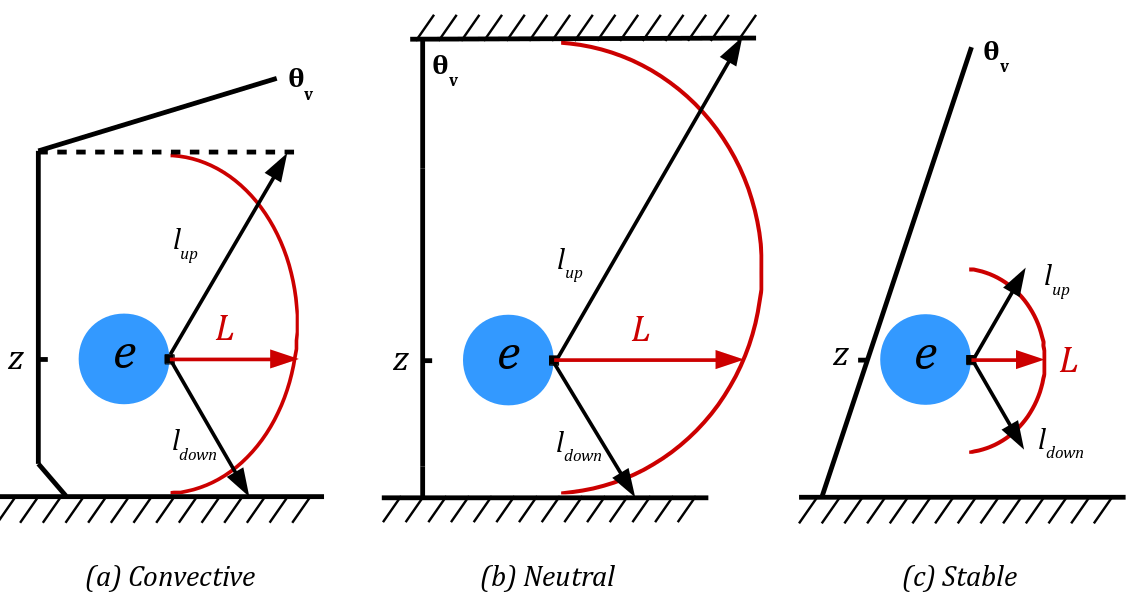
\includegraphics[width = 16cm]{\EPSDIR/BL89.png}
\caption{BL89 mixing length vertical profile (red) in convective, neutral and stable boundary layers.}
\label{fig:BL89}
\end{figure}

To improve the representation of turbulent mixing in neutral and stable boundary layers, RM17 (Rodier and Masson, 2017) adds a local vertical wind shear term to the buoyancy-based BL89 formulation :
\begin{equation}
\begin{split}
\int_z^{z+l_{up}} \left[\dfrac{g}{\theta_{vref}}(\theta_v (z) - \theta_v (z')) + C_0 \sqrt{e}S(z')\right]dz' = - e(z), \\
\int_{z-l_{down}}^z \left[\dfrac{g}{\theta_{vref}}(\theta_v (z') - \theta_v (z))+ C_0 \sqrt{e}S(z')\right]dz' = - e(z),
\end{split}
\label{eq:BS}
\end{equation}

where $C_0$ is a constant and $S(z')$ the local vertical wind shear:

\begin{equation}
S = \sqrt{\left(\dfrac{\partial \overline{u}}{\partial z}\right)^2 + \left(\dfrac{\partial \overline{v}}{\partial z}\right)^2}
\end{equation}

The shear term corresponds to the slowdown effect produced by the vertical decoupling of turbulent structures when the local shear is strong (Figure \ref{fig:shear}). This effect also depends on the average eddy size with larger eddies more decoupled.

\begin{figure}[!ht]
\centering
\noindent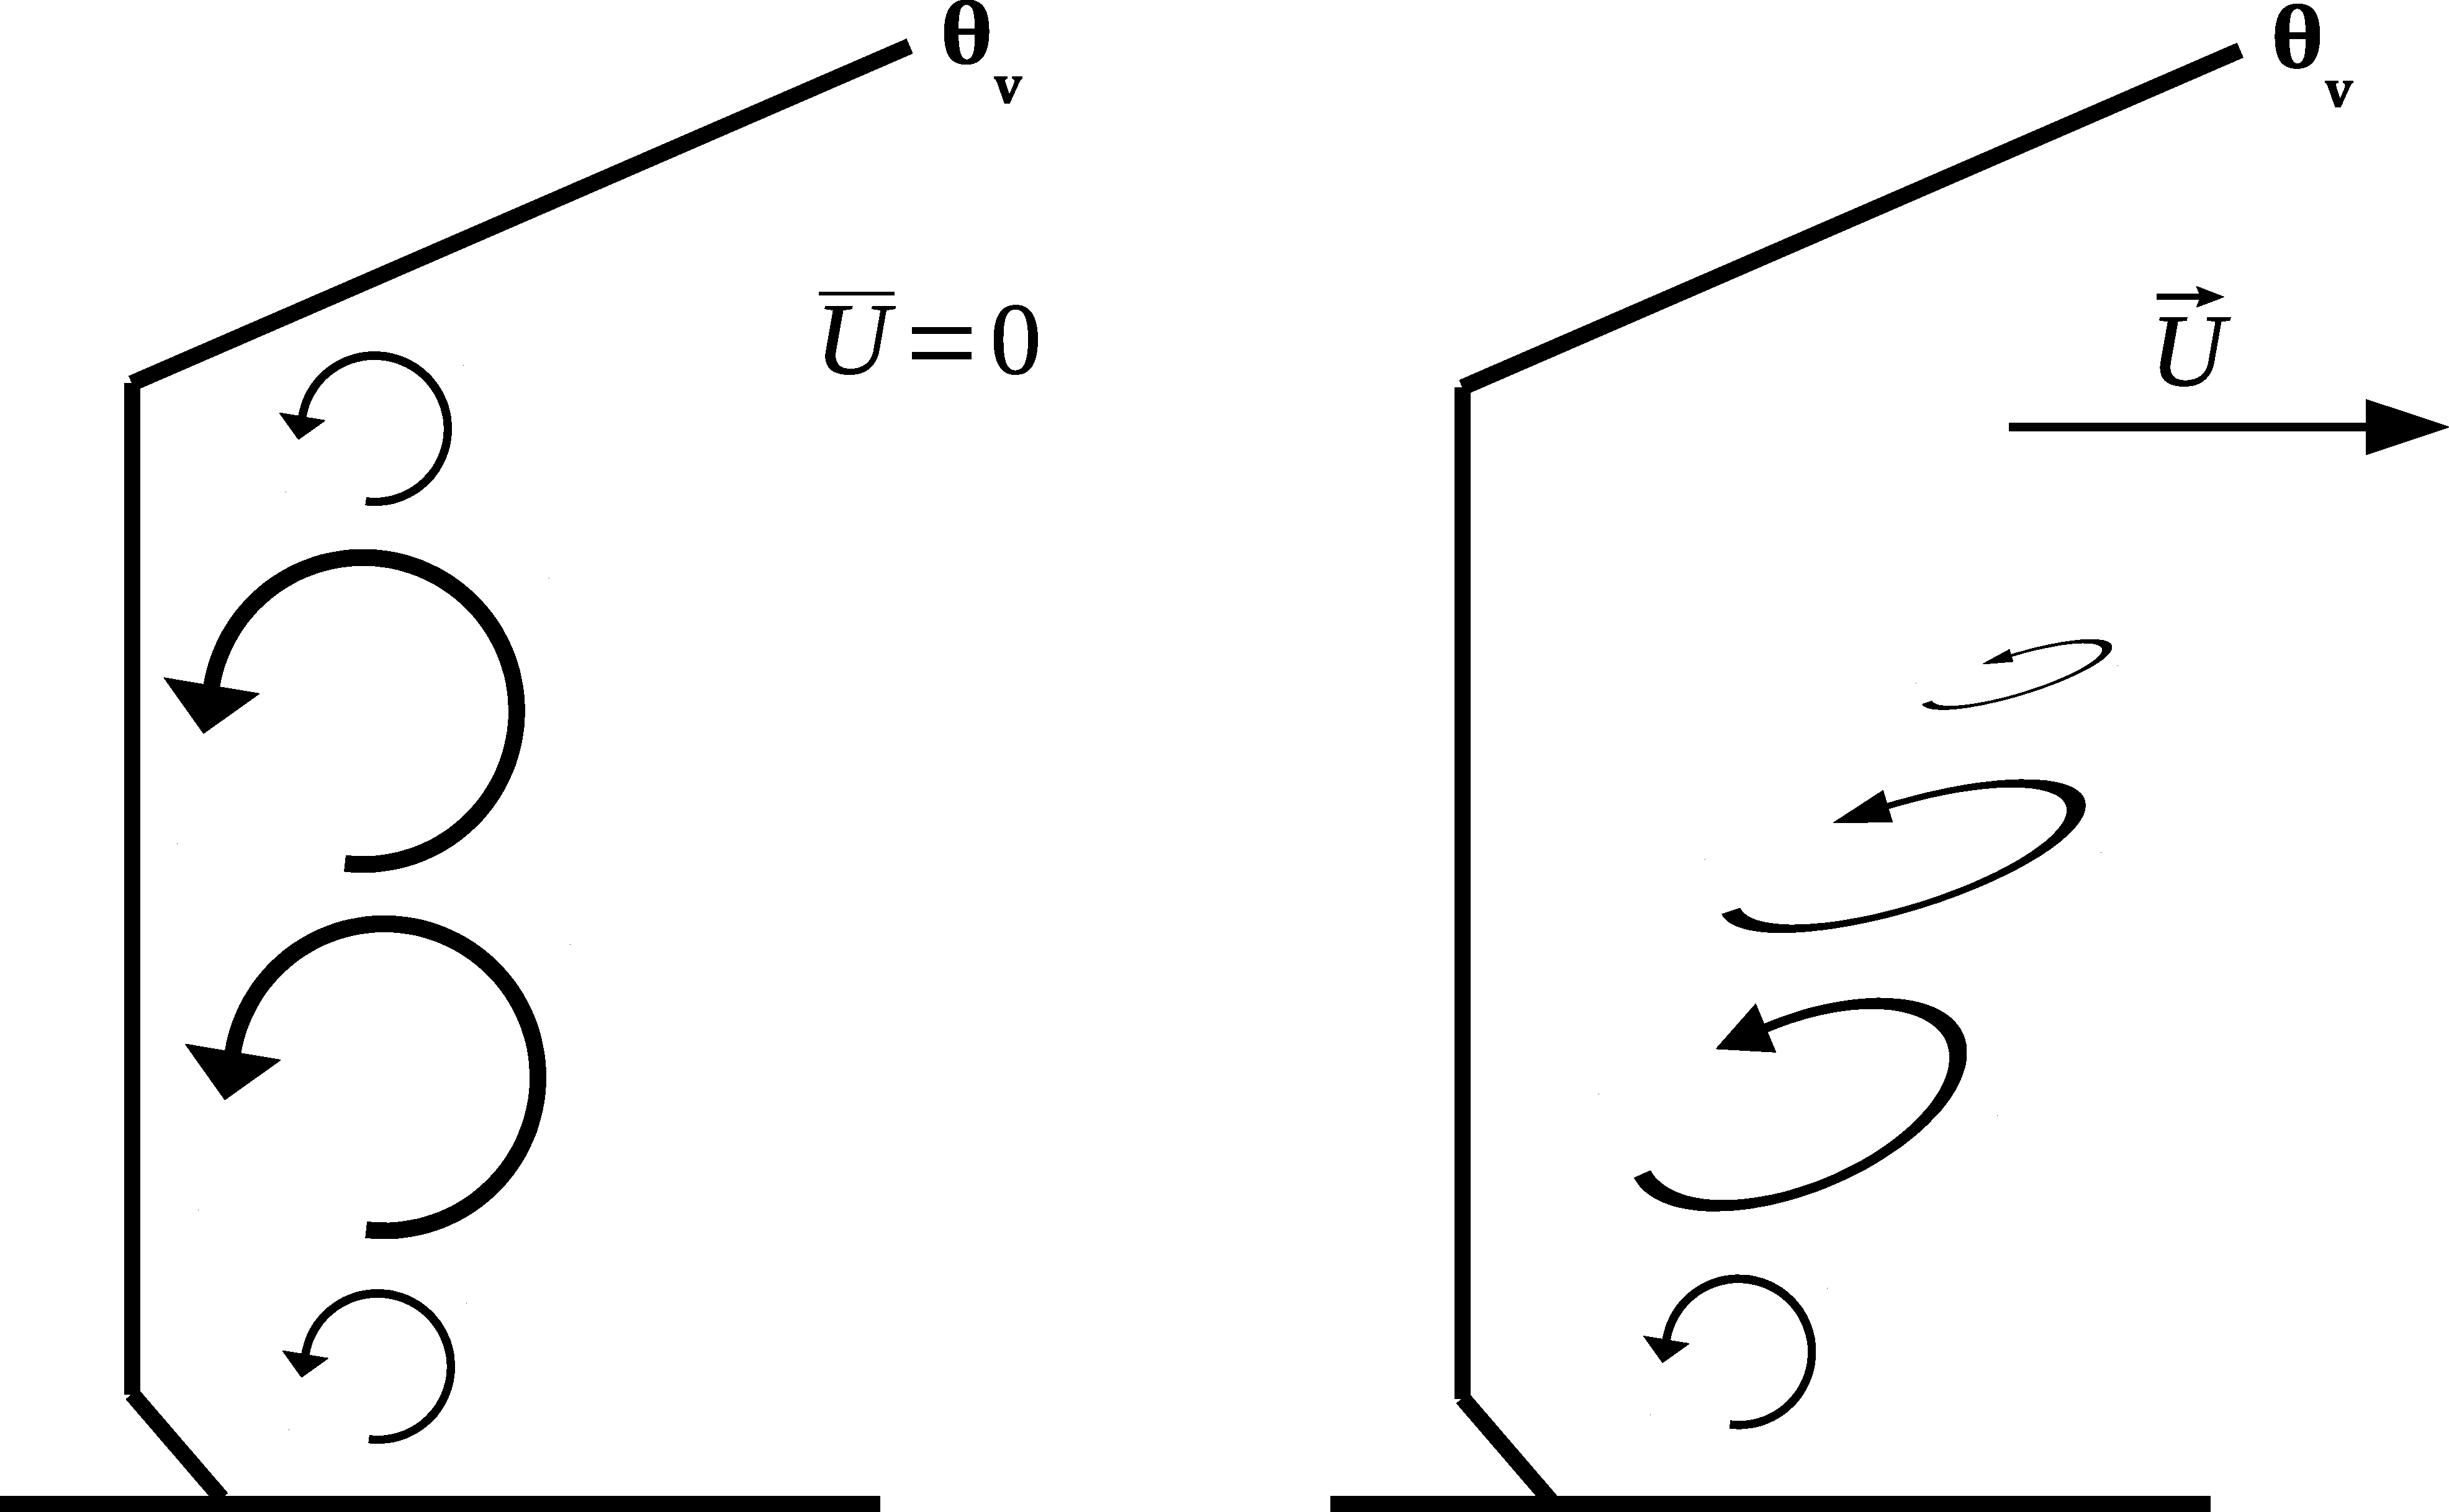
\includegraphics[width=8.5cm]{\EPSDIR/BS.jpg}
\caption{Schematic view of the effect of stratification and vertical wind shear on the reduction of the vertical mixing efficiency. Without wind shear (left), the turbulent structures are constrained by the distance to the surface and by the stratification. The presence of a wind shear (right) results in the stretching and vertical decoupling of the turbulent structures.}
\label{fig:shear}
\end{figure}

\subsection{Mixing length for the grey zone of turbulence}

This mixing length is adapted to the constraints of the hectometric-scale grey zone of turbulence for neutral and convective boundary layers. 
It combines a mixing length for mesoscale simulations $L_{RM17}$ (see above), where the turbulence is fully subgrid and a mixing length for Large-Eddy Simulations, where the coarsest turbulent eddies are explicitly resolved.
 
\begin{eqnarray}
	L_{\Delta}=(\Delta x \Delta y)^{1/2},
\end{eqnarray}

The mixing length $\mathfrak{L}$ is built for isotropic turbulence schemes, as well as schemes using the horizontal homogeneity assumption. $\mathfrak{L}$ is the minimum mixing length between the horizontal grid cell $L_{\Delta}$ and $L_{RM17}$: 

\begin{eqnarray}
	\mathfrak{L}=min(\alpha L_{\Delta}, L_{RM17}),
	\label{Eq1}
\end{eqnarray}

where $\alpha$ is a tuning parameter set to 0.5, according to the numerical experiments detailed in Honnert et al. (2021).

With this new mixing length, the turbulence scheme produces the right proportion between subgrid and resolved turbulent exchanges in Large Eddy Simulations, in the grey zone of turbulence, as well as at the mesoscale. This opens the way of using a single mixing length whatever the grid mesh of the atmospheric model, the evolution stage or the depth of the boundary layer.

\subsection{Qualitative behavior of the 1D dry system with BL length}
\paragraph{Critical Richardson number}
Let us write the 1D TKE evolution equation introducing into it the expressions
for the fluxes, and neglecting the turbulent transport for this particular case:
%PM 02/07/2001 D\E9but diverses retouches Pascal Marquet
\be
\frac {\partial e}{\partial t}=
\frac{4 L}{15 C_m} e^{\frac{1}{2}} (\frac {\partial U}{\partial z})^2
-\frac{g}{\theta_{v0}}\frac{2 L}{3 C_s} e^{\frac{1}{2}}
 \frac {\partial \theta}{\partial z}
 \left(1+C_1  \frac{L^2}{e} \frac{g}{\theta_{v0}}
       \frac {\partial \theta}{\partial z}
 \right)^{-1}
- C_{\epsilon} \frac{e^{\frac{3}{2}}}{L}
\ee

\noindent
where the term $(\,\,\,\,)^{-1}$ is the developed expression for $\phi_3$ in
1D dry mode. Introducing the value for BL in stable layers
($ L= \sqrt{\frac{2 e(z)}{\alpha \beta}}$) and defining the buoyancy as
$B=\beta \alpha$,

\be
\frac {\partial e}{\partial t}= e \left[
\frac {4 \sqrt{2}}{15 C_m} (\frac {\partial U}{\partial z})^2 \frac{1}{\sqrt{B}}
-\sqrt{B}\sqrt{2} \frac{2}{3 C_s} (\frac{1}{1+2C_1})
- \frac{C_{\epsilon}}{\sqrt{2}} \sqrt{B} \right]
\ee
%PM 02/07/2001 Fin diverses retouches Pascal Marquet\noindent

The critical Richardson number is the one that nullifies the previous equation,
\be
Ri_c= \frac{B}{(\frac {\partial U}{\partial z})^2}=
\frac  {\frac {4 \sqrt{2}}{15 C_m} }
       { \frac{2 \sqrt{2}}{3 C_s} (\frac{1}{1+2C_1}) + \frac{C_{\epsilon}}{\sqrt{2}}}
\ee

\noindent
and entering the values of the constants (RS81), $C_m=C_s=4, C_1=0.139,
C_{\epsilon}=0.7$, the critical Richardson of the 1D proposed scheme is
{\bf $Ri_c= 0.139$}.

\subsection{Mixing length in clouds}
From the masdev46 version a namelist {\tt NAM\_TURB\_CLOUD} allows us to differentiate the mixing length inside and outside a cloud, for the chosen model {\tt NMODEL\_CLOUD}.
Indeed, in a convective atmosphere, the cloud interface (but also inside the cloud)  undergoes a small scale instabilities of a few meters which enhances the mixing (Squire 1958; Klaassen and Clark 1985; Emanuel 1994). The clear sky mixing length cannot be sufficient to take into account this turbulence enhancement when the physical gradients are not resolved.
The proposed simple solution consists in chosen a specific cloud mixing length ({\tt CTURBLEN\_CLOUD}) which can be increased in the 3D turbulence scheme following an instability criterion. At each time step and in each horizontal direction, if a grid point satisfies all the following conditions:
\begin{itemize}
\item itself or its adjacent points are cloudy ($r_c+r_i>0.001$~g/kg);
\item G, the horizontal gradient of the non precipitating total water
($r_v+ r_c+r_i$) is strong enough ($|G|\leq 0.1$~g/kg/km);
\item G amplifies itself with time by advection, that is to say the
frontogenetic type term $Q=dG/dt$ is of the same sign as $G$.
\end{itemize}
The mixing length at this point which appears in the diffusion coefficient $K=L\sqrt{e}$ of the horizontal fluxes is multiplied by the coefficient $\alpha$, a linear function of $Q$ (averaged in both horizontal directions) between two limits to be prescribed in the namelist ($Q_{\rm min}$  and $Q_{\rm max}$), with a maximum $\alpha_{\rm max}$ also to choose (Fig.~\ref{coef_ampl_incloud}).
This local enhancement of the mixing length in clouds has been tested at resolutions of 2-3~km in a thunderstorm with extreme vertical velocities. With the following values, taken by default in the namelist, the vertical velocities and fluxes are reasonable compared to the high resolution simulation (400~m): $\alpha_{\rm max}=5$, $Q_{\rm min}=0.001$~g/kg/km/s,  $Q_{\rm max}=0.01$~g/kg/km/s.

\begin{figure}[!ht]
\centerline{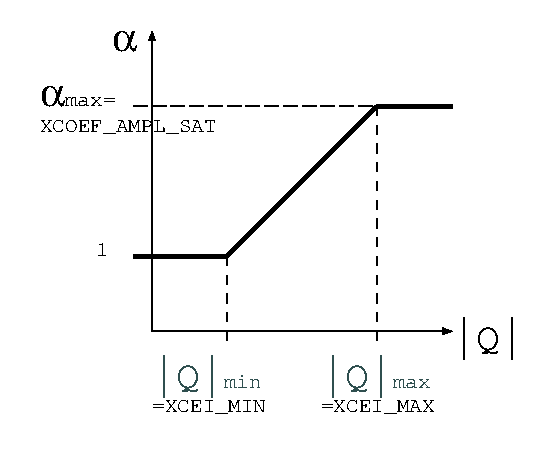
\includegraphics[width=10cm]{\EPSDIR/coef_ampl_incloud.eps}}
\caption{Coefficient $\alpha$ of in-cloud mixing length enhancement as function of the instability criterion $Q$.}
\label{coef_ampl_incloud}
\end{figure}

\section{Closure by dissipation equation}

This is an alternative way to close the system (Hanjalic and Launder 1972),
obtaining a value for L from an additional prognostic equation. The most
popular method is the so-called $k-\epsilon$ approach, in the
engineering vocabulary, where $k$ stands for the TKE and $\epsilon$ for
its dissipation.

The prognostic equation for $\epsilon$ reads
\begin{equation}
\frac {D \epsilon}{D t}=P(\epsilon)-D(\epsilon) + T(\epsilon),
\end{equation}
where the source terms are defined as
\begin{eqnarray}
P(\epsilon)&=&-C_{\epsilon 1} \frac {\epsilon}{e} \overline{u_i' u_k'}
\frac{\partial U_i}{\partial x_k}=C_{\epsilon 1} \frac {\epsilon}{e}
P(e),\\
D(\epsilon)&=&C_{\epsilon 2} \frac {\epsilon ^2}{e},\\
T(\epsilon)&=&-\frac{\partial}{\partial x_j}
(-c_{\epsilon} \frac{e}{\epsilon} \overline{u_j' u_k'}
\frac{\partial \epsilon}{\partial x_k})=-\frac{\partial
\overline{w' \epsilon'}}{\partial z}
\end{eqnarray}

However, in the presence of stratification Duynkerke (1988) showed that
it is necessary to use
\begin{equation}
P(\epsilon)=S+\max(0,B)+\max(0,T(e))
\end{equation}
where S, B and T stand for the shear production, buoyancy production and
turbulent transport in the TKE evolution equation.\\
\nocite{Han_Laun72} \nocite{Duynkerke88}

Knowing $\epsilon$, the mixing length is recovered by inverting the
Kolmogorov relation
\begin{equation}
\epsilon=C_{\epsilon} \frac{e^{\frac{3}{2}}}{L}.
\end{equation}

Although it has been coded, this formulation is not yet giving satisfactory
results, and is not currently available.


%\chapter{Inclusion of a dissipative heating term in M\'esoNH}

%{\em by J.-P. Pinty}

\section{Conservation of the energy in Meso-NH}

The examination of the energy conservation in a model of atmosphere is a very
difficult task. In numerical models, this question is even untractable. However,
a recent study of Blister and Emanuel (1998) pointed out that a thermodynamic
energy arising from dissipative heating is always neglected in mesoscale
models. Indeed this should not be the case when simulating hurricanes or very turbulent 
flows as omitting this term may lead to an appreciable underestimation of the intensity of 
tropical cyclones.

It is well known that the frictional dissipation of kinetic energy occurs at 
molecular scales where it is ultimately converted into thermal energy or heat.
As numerical models perform a time integration of the "mean" (grid-averaged)
momentum equations, an additional equation is used to parameterize the sub-grid 
scale motions and their up-scaling fluxes. 

The momentum conservation equation is rewritten here for convenience:
\begin{eqnarray}
\label{NewEqMomentum}
\dfrac{\partial}{\partial t}(\rho_{d\,eff} {U_i})
+\dfrac{\partial}{\partial x_j} (\rho_{d\,eff} {U_i} \cdot {U_j} )
%+\rho_{d\,eff} C_{pd} \theta_{v}\overbar{ \nabla} \Pi '
+ \rho_{d\,eff} {\cal F}_{\Pi}
+ \rho_{d\,eff}  \delta_{i3} g \dfrac{\theta_v-\theta_{v\,ref}}{\theta_{v\,ref}}
+ \rho_{d\,eff} f \epsilon_{ij3} {U_j} = & \nonumber\\
+ \nu \dfrac{\partial^2}{\partial x_j^2} (\rho_{d\,eff} {U_i}) 
+ \rho_{d\,eff} {\cal F} , \qquad &
\end{eqnarray}

\noindent where $\rho_{d\,eff} \vec{{\cal F}_{\Pi}}$ is the pressure gradient force, which
takes different forms in the three anelastic systems:

%
\parbox{12cm}{
\begin{displaymath}
\rho_{d\,eff} \vec{{\cal F}_{\Pi}} =  \left\{
\begin{array}{l@{\quad}cc}
\rho_{d\,eff}  \vec{ \nabla}(C_{pd} \theta_{v\,ref} \Pi '),
                                        & \quad &\mbox{(Lipps-Hemler)}\\
\rho_{d\,eff} C_{pd} \theta_{v\,ref} \vec{ \nabla} \Pi ',
                                                & \quad &\mbox{(Mod. Anelastic  Eq.)} \\
\rho_{d\,eff} C_{pd} \theta_{v} \vec{ \nabla} \Pi '. & \quad  &\mbox{(Durran)}
\end{array}
\right.
\end{displaymath}
}
\hfill
\parbox{1cm}{
\begin{eqnarray}
\ \label{LhgradP} \\ \label{MAEgradP}   \\ \label{DUgradP}
\end{eqnarray}
}
%

Expansion of the mean and turbulent parts ($U_i=\overline{U_i}+u'_i$) and
applying Reynolds averaging rules on the momentum equation leads to
\begin{eqnarray}
\label{NewMeanEqMomentum}
\dfrac{\partial}{\partial t}(\rho_{d\,eff} \overline{U_i})
+\dfrac{\partial}{\partial x_j} (\rho_{d\,eff} \overline{U_i} \cdot \overline{U_j} )
+ \rho_{d\,eff} \overline{\cal F}_{\Pi}
+ \rho_{d\,eff}  \delta_{i3} g \dfrac{\overline{\theta_v}-\theta_{v\,ref}}{\theta_{v\,ref}}
+ \rho_{d\,eff} f \epsilon_{ij3} \overline{U_j} = & \nonumber\\
+ \nu \dfrac{\partial^2}{\partial x_j^2} (\rho_{d\,eff} \overline{U_i}) -\dfrac{\partial}{\partial x_j} (\rho_{d\,eff} \overline{u'_i u'_j})               
+ \rho_{d\,eff} \overline{\cal F} , \qquad &
\end{eqnarray}

\noindent where $\rho_{d\,eff} \overline{u'_i u'_j}$ is the turbulent mean 
flux. The conservation equation of the turbulent part is obtained by 
subtracting equation (\ref{NewMeanEqMomentum}) to (\ref{NewEqMomentum})
\begin{eqnarray}
\label{NewTurbEqMomentum}
\dfrac{\partial}{\partial t}(\rho_{d\,eff} {u'_i})
+\dfrac{\partial}{\partial x_j} (\rho_{d\,eff} {u'_i} \cdot \overline{U_j} )
+ \rho_{d\,eff} ({\cal F}_{\Pi})'
+ \rho_{d\,eff}  \delta_{i3} g \dfrac{\theta'_v}{\theta_{v\,ref}}
+ \rho_{d\,eff} f \epsilon_{ij3} {u'_j} = 
 & \nonumber\\
- \dfrac{\partial}{\partial x_j} (\rho_{d\,eff} u'_i u'_j) 
- \dfrac{\partial}{\partial x_j} (\rho_{d\,eff} \overline{U_i} \cdot {u'_j} )
\qquad  & \nonumber\\
+ \nu \dfrac{\partial^2}{\partial x_j^2} (\rho_{d\,eff} {u'_i}) 
+ \dfrac{\partial}{\partial x_j} (\rho_{d\,eff} \overline{u'_i u'_j}) 
+ \rho_{d\,eff} ({\cal F})' , \qquad &
\end{eqnarray}

Multiplying equation (\ref{NewMeanEqMomentum}) by $\overline{U_i}$ leads to the
mean kinetic energy equation with 
$K=\rho_{d\,eff} (\overline{U_i} \cdot \overline{U_i}/2)$
and using the anelastic continuity equation 
$\partial/\partial x_i (\rho_{d\,eff} \overline{U_i})=0$ of the mean flow
\begin{eqnarray}
\label{NewMeanEqKenergy}
\dfrac{\partial}{\partial t} K
+\dfrac{\partial}{\partial x_j} (K \cdot \overline{U_j} )
+ \Big[\rho_{d\,eff} \overline{\cal F}_{\Pi}
+ \rho_{d\,eff}  \delta_{i3} g \dfrac{\overline{\theta_v}-\theta_{v\,ref}}{\theta_{v\,ref}}
+ \rho_{d\,eff} f \epsilon_{ij3} \overline{U_j} \Big] \cdot \overline{U_i} = & \nonumber\\
+\Big[\nu \dfrac{\partial^2}{\partial x_j^2} (\rho_{d\,eff} \overline{U_i}) -\dfrac{\partial}{\partial x_j} (\rho_{d\,eff} \overline{u'_i u'_j})               
+ \rho_{d\,eff} \overline{\cal F} \Big] \cdot \overline{U_i} , \qquad &
\end{eqnarray}
\noindent while multiplying equation (\ref{NewTurbEqMomentum}) by $u'_i$ and 
averaging after rearrangement leads to the turbulent kinetic energy equation 
with $TKE=\rho_{d\,eff} (\overline{u'_iu'_i}/2)$ (the anelastic continuity 
equation 
$\partial/\partial x_i (\rho_{d\,eff} {u'_i})=0$ of the turbulent flow is 
used)
\begin{eqnarray}
\label{NewTurbEqTKE}
\dfrac{\partial}{\partial t} TKE
+\dfrac{\partial}{\partial x_j} (TKE \cdot \overline{U_j} )
+ \rho_{d\,eff} \overline{({\cal F}_{\Pi})'u'_i}
+ \rho_{d\,eff}  \delta_{i3} g \dfrac{\overline{\theta'_v u'_i}}{\theta_{v\,ref}}
+ \rho_{d\,eff} f \epsilon_{ij3} \overline{u'_i u'_j} = & \nonumber\\
- \overline{u'_i\dfrac{\partial}{\partial x_j} (\rho_{d\,eff} u'_i u'_j)} 
- \overline{u'_i \dfrac{\partial}{\partial x_j} (\rho_{d\,eff} \overline{U_i} \cdot {u'_j} )}
+ \nu \overline{u'_i \dfrac{\partial^2}{\partial x_j^2} (\rho_{d\,eff} {u'_i})} 
+ \rho_{d\,eff} \overline{({\cal F})' u'_i} , \qquad &
\end{eqnarray}
\noindent which is equivalent to:
\begin{eqnarray}
\label{NewNewTurbEqTKE}
\dfrac{\partial}{\partial t} TKE
+\dfrac{\partial}{\partial x_j} (TKE \cdot \overline{U_j} )
+ \rho_{d\,eff} \overline{({\cal F}_{\Pi})'u'_i}
+ \rho_{d\,eff}  \delta_{i3} g \dfrac{\overline{\theta'_v u'_i}}{\theta_{v\,ref}}
+ \rho_{d\,eff} f \epsilon_{ij3} \overline{u'_i u'_j} = & \nonumber\\
- \dfrac{\partial}{\partial x_j} \overline{TKE' u'_j}
- (\rho_{d\,eff} \overline{u'_i u'_j}) \dfrac{\partial}{\partial x_j} \overline{U_i} 
\qquad  & \nonumber\\
+ \dfrac{\nu}{\rho_{d\,eff}} \Big[ \dfrac{\partial}{\partial x_j} \rho_{d\,eff} \Big[ \dfrac{\partial}{\partial x_j} TKE\Big] \Big]
- \dfrac{\nu}{\rho_{d\,eff}} \Big[ \overline{\dfrac{\partial}{\partial x_j} \Big( \rho_{d\,eff} u'_i\Big)} \Big]^2
+ \rho_{d\,eff} \overline{({\cal F})' u'_i} , \qquad &
\end{eqnarray}
\noindent where the flux-like notation $\overline{TKE' u'_j}$ stands for 
$\rho_{d\,eff} \overline{(u'_iu'_i/2) u'_j}$. In the rhs of equation 
(\ref{NewNewTurbEqTKE}), the $TKE$-diffusion term, proportional to the molecular
viscosity $\nu$, is split in two terms. The "Laplacian" term is a redistribution
term which is often neglected. The second term is much larger and is always 
negative (minus a squared quantity). This term corresponds to the viscous 
dissipation rate $\varepsilon$ 
\begin{equation}
\label{DissipationTerm}
\varepsilon_{TKE} = \dfrac{\nu}{\rho_{d\,eff}} \Big[ \overline{\dfrac{\partial}{\partial x_j} \Big( \rho_{d\,eff} u'_i\Big)} \Big]^2,
\end{equation}
Adding equations (\ref{NewMeanEqKenergy}) and (\ref{NewNewTurbEqTKE}) gives the
evolution of the total kinetic energy equation ($K + TKE$) which explicitly 
contains the momentum
dissipation term $\varepsilon$. By virtue of the total energy conservation, a
counterpart dissipative energy must be added to the thermodynamic equation. 
This can be simply done by the introduction of a dissipative heating term of
the form
\begin{eqnarray}
\label{NewThequa}
\dfrac{\partial}{\partial t}(\rho_{d\,eff} \theta)  + \vec{ \nabla} \cdot
(\rho_{d\,eff} \theta \;\vec{U})
= 
%% \rho_{d\,eff} \left[ {R_d+r_vR_v\over R_d}{C_{pd} \over C_{ph}}-1 \right]
%% {\theta \over \Pi_{ref}} w {\partial \Pi_{ref} \over \partial z}
%% \nonumber \\
%% + {\rho_{d\,eff}\over \Pi_{ref} C_{ph}} \left[
%%  L_m {D(r_i+r_s+r_g+r_h)\over Dt} - L_v {Dr_v\over Dt} + {\cal H}  \right].
\cdots + \dfrac{\rho_{d\,eff} \varepsilon_{e}}{\Pi_{ref} C_{ph}}.
\end{eqnarray}
The turbulence scheme in Meso-NH is based on a turbulent kinetic
equation of $e$ defined as $e=TKE/\rho_{d\,eff}$. Most of the second order 
terms in equation (\ref{NewNewTurbEqTKE}) including 
$\varepsilon_{TKE}= \varepsilon_{e}\times \rho_{d\,eff}$ are parameterized 
according to Cuxart et al. (2000).

\section{Terrain-following coordinate system}

In Meso-NH, the coordinate system is not Cartesian, in order to account
for steep terrain, and the sphericity of the earth. As explained in Part I,
Chapters 3 and 4 on coordinate systems and discretization, respectively,
we use a $(\overline{x},\overline{y},\overline{z})$ coordinate
system, and the contravariant components of the velocity. By inserting these
various elements in the basic equations, the form of the turbulent terms
is readily obtained. For instance, the turbulent terms in the equation
for the mean $x$ momentum component read
\begin{eqnarray}
{\partial \tilde{\rho} \overline{u}\over \partial t}=\cdots
&-&\left[\frac{\partial}{\partial \overline{x}}(\tilde{\rho}
\frac{\overline{u'u'}}{d_{xx}})+\frac{\partial}{\partial \overline{y}}
(\tilde{\rho}\frac{\overline{u'v'}}{d_{yy}})+
\frac{\partial}{\partial \overline{z}}(\tilde{\rho}\frac{\overline{w'u'}}
{d_{zz}}-\tilde{\rho}\overline{u'u'}\frac{d_{zx}}{d_{xx}d_{zz}}
-\tilde{\rho}\overline{v'u'}\frac{d_{zy}}{d_{yy}d_{zz}}) \right ]\nonumber\\
&+&\overline{u'v'}\frac{\tilde{\rho}cos\gamma}{rcos\varphi}(sin \varphi -K)
+\overline{v'v'}\frac{\tilde{\rho}sin\gamma}{rcos\varphi}(sin \varphi -K)
-\tilde{\rho}\frac{\overline{u'w'}}{r}.
\end{eqnarray}
The last line of this expression  arises from the curvature terms
generated by the sphericity of the Earth.
In the following, we will assume that these sphericity terms have negligible
contributions on the turbulence, and therefore ignore them.

On the other hand, we should stress that the $(u,v,w)$ used in the equations
are still the Cartesian components of the velocity.
So, the terms that the turbulence scheme will supply to Meso-NH are
\begin{eqnarray}
\frac{\partial }{\partial t}(\tilde{\rho}u)&=
\cdots&-\left[\frac{\partial}{\partial \overline{x}}(\tilde{\rho}
\frac{\overline{u'u'}}{d_{xx}})+\frac{\partial}{\partial \overline{y}}(\tilde
{\rho}\frac{\overline{u'v'}}{d_{yy}})+
\frac{\partial}{\partial \overline{z}}(\tilde{\rho}\frac{\overline{w'u'}}
{d_{zz}}-\tilde{\rho}\overline{u'u'}\frac{d_{zx}}{d_{xx}d_{zz}}
-\tilde{\rho}\overline{v'u'}\frac{d_{zy}}{d_{yy}d_{zz}}) \right ],\nonumber\\
\frac{\partial }{\partial t}(\tilde{\rho}v)&=
\cdots&-\left[\frac{\partial}{\partial \overline{x}}(\tilde{\rho}
\frac{\overline{u'v'}}{d_{xx}})+\frac{\partial}{\partial \overline{y}}(\tilde
{\rho}\frac{\overline{v'v'}}{d_{yy}})+
\frac{\partial}{\partial \overline{z}}(\tilde{\rho}\frac{\overline{v'w'}}
{d_{zz}}-\tilde{\rho}\overline{u'v'}\frac{d_{zx}}{d_{xx}d_{zz}}
-\tilde{\rho}\overline{v'v'}\frac{d_{zy}}{d_{yy}d_{zz}}) \right ],\nonumber\\
\frac{\partial }{\partial t}(\tilde{\rho}w)&=
\cdots&-\left[\frac{\partial}{\partial \overline{x}}(\tilde{\rho}
\frac{\overline{w'u'}}{d_{xx}})+\frac{\partial}{\partial \overline{y}}(\tilde
{\rho}\frac{\overline{w'v'}}{d_{yy}})+
\frac{\partial}{\partial \overline{z}}(\tilde{\rho}\frac{\overline{w'w'}}
{d_{zz}}-\tilde{\rho}\overline{u'w'}\frac{d_{zx}}{d_{xx}d_{zz}}
-\tilde{\rho}\overline{v'w'}\frac{d_{zy}}{d_{yy}d_{zz}}) \right ],\nonumber \\
\frac{\partial }{\partial t}(\tilde{\rho}s)&=
\cdots&-\left[\frac{\partial}{\partial \overline{x}}(\tilde{\rho}
\frac{\overline{s'u'}}{d_{xx}})+\frac{\partial}{\partial \overline{y}}(\tilde
{\rho}\frac{\overline{s'v'}}{d_{yy}})+
\frac{\partial}{\partial \overline{z}}(\tilde{\rho}\frac{\overline{w's'}}
{d_{zz}}-\tilde{\rho}\overline{u's'}\frac{d_{zx}}{d_{xx}d_{zz}}
-\tilde{\rho}\overline{v's'}\frac{d_{zy}}{d_{yy}d_{zz}}) \right ],\nonumber
\end{eqnarray}
where $s$ is any scalar.

In addition, all the gradients appearing in the flux formulation and in the
TKE prognostic equation must be evaluated in the model coordinate system by
the chain rule (see below).

%%%%%%%%%%%%%%%%%%%%%%%%%%%%%%%%%%%%%%%%%%%%%%%%%%%%%%%%%%%%%%%%%%%%%%%%%%%%%

\section{Spatial discretization}
The location of the different variables on the computation grid is shown in
Fig.~\ref{maille}. All the variables shown share the same index values i,j,k.
In the following, we will use the Schuman discretization operators, as defined
in Part I, Chapter 4 on discretization (section 4.3).

\begin{figure}[!ht]
\centerline{\includegraphics[]{\EPSDIR/maille.eps}}
\caption{Location of variables on the grid for turbulence computation.}
\label{maille}
\end{figure}

The discretized form of the turbulence terms in the main equations reads
\begin{eqnarray}
\delta_t \left [ \overline{(\overline{\tilde{\rho}}^x u)}^t \right ]=
\cdots&-&\delta_x(\tilde{\rho}\frac{\overline{u'u'}}{\overline{d_{xx}}^x})
-\delta_y(\overline{\tilde{\rho}}^{x,y}\frac{\overline{u'v'}}{\overline{d_{yy}
}^x}) \nonumber \\
&-&\delta_z(\overline{\tilde{\rho}}^{z,x}\frac{\overline{w'u'}}{\overline
{d_{zz}}^x}
-\overline{\tilde{\rho}}^{z,x}\overline{\overline{u'u'}}^{z,x}
\frac{d_{zx}}{\overline{d_{xx}}^z\overline{d_{zz}}^x}
-\overline{\tilde{\rho}}^{z,x}\overline{\overline{v'u'}}^{z,y}
\frac{\overline{d_{zy}}^{x,y}}{\overline{d_{yy}}^{x,y,z}\overline{d_{zz}}^x}
) \nonumber\\
\delta_t \left [ \overline{(\overline{\tilde{\rho}}^y v)}^t \right ]=
\cdots&-&\delta_x(\overline{\tilde{\rho}}^{x,y}\frac{\overline{u'v'}}
{\overline{d_{xx}}^y})
-\delta_y(\tilde{\rho}\frac{\overline{v'v'}}{\overline{d_{yy}}^y})
\nonumber \\
&-&\delta_z(\overline{\tilde{\rho}}^{z,y}\frac{\overline{w'v'}}{\overline
{d_{zz}}^y}
-\overline{\tilde{\rho}}^{z,y}\overline{\overline{u'v'}}^{z,x}
\frac{\overline{d_{zx}}^{y,x}}{\overline{d_{xx}}^{xyz}\overline{d_{zz}}^y}
-\overline{\tilde{\rho}}^{z,y}\overline{\overline{v'v'}}^{z,y}
\frac{d_{zy}}{\overline{d_{yy}}^z\overline{d_{zz}}^y}
) \nonumber\\
\delta_t \left [ \overline{(\overline{\tilde{\rho}}^z w)}^t \right ]=
\cdots&-&\delta_x(\overline{\tilde{\rho}}^{z,x}\frac{\overline{u'w'}}
{\overline{d_{xx}}^z})
-\delta_y(\overline{\tilde{\rho}}^{z,y}\frac{\overline{v'w'}}{\overline{d_{yy}
}^z})
\nonumber \\
&-&\delta_z(\tilde{\rho}\frac{\overline{w'w'}}{\overline{d_{zz}}^z}
-\tilde{\rho}\overline{\overline{u'w'}}^{z,x}
\frac{\overline{{d_{zx}}^{x,z}}}{\overline{d_{xx}}^x\overline{d_{zz}}^z}
-\tilde{\rho}\overline{\overline{v'w'}}^{y,z}
\frac{\overline{d_{zy}}^{y,z}}{\overline{d_{yy}}^{x}\overline{d_{zz}}^z}
) \nonumber\\
\delta_t \left [ \overline{(\tilde{\rho} s)}^t \right ]=
\cdots&-&\delta_x(\overline{\tilde{\rho}}^x\frac{\overline{u's'}}{d_{xx}})
-\delta_y(\overline{\tilde{\rho}}^y\frac{\overline{v's'}}{d_{yy}})
\nonumber \\
&-&\delta_z(\overline{\tilde{\rho}}^z\frac{\overline{w's'}}{d_{zz}}
-\overline{\tilde{\rho}}^z\overline{\overline{u's'}}^{z,x}
\frac{\overline{d_{zx}^x}}{\overline{d_{xx}}^{z,x}d_{zz}}
-\overline{\tilde{\rho}}^z\overline{\overline{v's'}}^{z,y}
\frac{\overline{d_{zy}}^y}{\overline{d_{yy}}^{z,y}d_{zz}}  )
\label{discturb}
\end{eqnarray}
\\

Here, we have assumed that the time discretization is fully explicit, and all
the terms on the right hand side are taken at time $t-\Delta t$. As
explained in the final section however, we allow for some degree of implicitness
in the time discretization of the purely vertical diffusion terms, in order
to allow for longer time steps when the model is used in meso-scale mode.
\\

In (\ref{discturb}), we still use the expression of the
turbulent fluxes in the Cartesian frame. Those must be expressed as a function
of the gradients of the mean variables in the Cartesian frame. To ease this
formulation, we have developed 15 different "Cartesian gradient operators",
depending of the direction in which the gradient is taken, and the precise
locations on the grid where the  information is available. The generic notation
for these operators is $GX_i\_A\_B$: $X_i$ refers to the (Cartesian) direction
where the gradient is taken, $A$ to the variable location, and $B$ to the
location where the gradients must be known. The detailed expression of these
operators is the following.
\\
\\
\noindent
1) Gradients at mass points for variables located at mass points:
\begin{eqnarray}
\frac{\partial \bullet}{\partial x}&=
\frac{1}{\overline{d_{xx}}^x}\left[ \delta_x \overline{\bullet}^x -
\overline{\left({\overline{d_{zx}}^x \delta_z \bullet \over d_{zz}}\right) }^z
\right]
&\equiv GX\_M\_M
\nonumber\\
\frac{\partial \bullet}{\partial y}&=
\frac{1}{\overline{d_{yy}}^y}\left[ \delta_y \overline{\bullet}^y -
\overline{\left({\overline{d_{zy}}^y \delta_z \bullet \over d_{zz}}\right) }^z
\right]
&\equiv GY\_M\_M
\nonumber\\
\frac{\partial \bullet}{\partial z}&=
\overline{\left( {\delta_z \bullet \over d_{zz} } \right) }^z
&\equiv GZ\_M\_M
\end{eqnarray}

\noindent
2) Gradients at wind points for variables located at mass points:
($\overline{u_i'\theta'}\Longleftrightarrow \frac{\partial \theta}{\partial x_i}$)
\begin{eqnarray}
\frac{\partial \bullet}{\partial x}&=
\frac{1}{d_{xx}}\left[ \delta_x \bullet -
\overline{\left({ d_{zx}\overline{\delta_z \bullet}^x \over d_{zz}}\right)}^z
\right]
&\equiv GX\_M\_U
\nonumber\\
\frac{\partial \bullet}{\partial y}&=
\frac{1}{d_{yy}}\left[ \delta_y \bullet -
\overline{\left({ d_{zy}\overline{\delta_z \bullet}^y \over d_{zz}}\right)}^z
\right]
&\equiv GY\_M\_V
\nonumber\\
\frac{\partial \bullet}{\partial z}&=
\frac{1}{d_{zz}} \delta_z \bullet
&\equiv GZ\_M\_W
\end{eqnarray}

\noindent
3) Gradients at mass points of variables located at wind points:
($\overline{u_i'^2} \Longleftrightarrow \frac{\partial u_i}{\partial x_i}$
unsummed)
\begin{eqnarray}
\frac{\partial \bullet}{\partial x}&=
\frac{1}{\overline{d_{xx}}^x}\left[ \delta_x \bullet -
\overline{\left({\overline{d_{zx}\delta_z \bullet}^x \over d_{zz}}\right)}^z
\right]
&\equiv GX\_U\_M
\nonumber\\
\frac{\partial \bullet}{\partial y}&=
\frac{1}{\overline{d_{yy}}^y}\left[ \delta_y \bullet -
\overline{\left({\overline{d_{zy}\delta_z \bullet}^y \over d_{zz}}\right)}^z
\right]
&\equiv GY\_V\_M
\nonumber\\
\frac{\partial \bullet}{\partial z}&=
\frac{1}{\overline{d_{zz}}^z} \delta_z \bullet
&\equiv GZ\_W\_M
\end{eqnarray}

\noindent
4) Gradients at vorticity points for variables located at wind points:
($\overline{u_i'u_j'} \Longleftrightarrow
\frac{\partial u_i}{\partial x_j}\,,\frac{\partial u_j}{\partial x_i}$)\\
For gradients localized at point UV:
\begin{eqnarray}
\frac{\partial \bullet}{\partial x}&=
\frac{1}{\overline{d_{xx}}^y}\left[ \delta_x \bullet -
\overline{\overline{\left({\delta_z\bullet \over \overline{d_{zz}}^y}\right)}^x
\overline{d_{zx}}^y }^z \right]
&\equiv GX\_V\_UV
\nonumber\\
\frac{\partial \bullet}{\partial y}&=
\frac{1}{\overline{d_{yy}}^x}\left[ \delta_y \bullet -
\overline{\overline{\left({\delta_z\bullet \over \overline{d_{zz}}^x}\right)}^y
\overline{d_{zy}}^x }^z \right]
&\equiv GY\_U\_UV
\end{eqnarray}

\noindent
For gradients localized at point UW:
\begin{eqnarray}
\frac{\partial \bullet}{\partial x}&=
\frac{1}{\overline{d_{xx}}^z}\left[ \delta_x \bullet -
\overline{\left({\overline{\delta_z\bullet}^z \over d_{zz}}\right)}^x d_{zx}
\right]
&\equiv GX\_W\_UW
\nonumber\\
\frac{\partial \bullet}{\partial z}&=
\frac{\delta_z\bullet}{\overline{d_{zz}}^x}
&\equiv GZ\_U\_UW
\end{eqnarray}

\noindent
For gradients localized at point VW:
\begin{eqnarray}
\frac{\partial \bullet}{\partial y}&=
\frac{1}{\overline{d_{yy}}^z}\left[ \delta_y \bullet -
\overline{\left({\overline{\delta_z\bullet}^z \over d_{zz}}\right)}^y d_{zy}
\right]
&\equiv GY\_W\_VW
\nonumber\\
\frac{\partial \bullet}{\partial z}&=
\frac{\delta_z\bullet}{\overline{d_{zz}}^y}
&\equiv GZ\_V\_VW
\end{eqnarray}

\smallskip
Making use of these operators, the discretized form of the turbulent
fluxes in the Cartesian frame reads as follows:
\begin{eqnarray}
\overline{u_i'\,u_j'}&=&\frac{2}{3}\delta_{ij}\,\overline{e}^{x_i,x_j}
 -\frac{4}{15} \frac{\overline{L}^{x_i,x_j}}{C_m} \overline{e^
{\frac{1}{2}}}^{x_i,x_j}
[ GX_j\_U_i\_U_iU_j(u_i)+GX_i\_U_j\_U_iU_j(u_j)\nonumber \\
&-&\frac{2}{3}\delta_{ij}\sum_{m=1}^{3} GX_m\_U_m\_U_iU_j(u_m) ] \\
\overline{u_i'\theta'}&=&-\frac{2}{3}\frac{\overline{L}^{x_i}}{C_s}
\overline{e^{\frac{1}{2}}}^{x_i}
GX_i\_M\_U\_i(\theta) \phi_i\\
\overline{u_i'r_v'}&=&-\frac{2}{3}\frac{\overline{L}^{x_i}}{C_s}
\overline{e^{\frac{1}{2}}}^{x_i}
GX_i\_M\_U\_i(r_v) \psi_i\\
\overline{\theta'r_v'}&=&C_2 L^2
\sum_{m=1}^{3}GX_m\_M\_M(\theta)GX_m\_M\_M(r_v)(\overline{\phi_m}^z
+\overline{\psi_m}^z)\\
\overline{\theta'^2}&=&C_1 L^2
\sum_{m=1}^{3}(GX_m\_M\_M(\theta))^2)\overline{\phi_m}^z\\
\overline{r_v'^2}&=&C_1 L^2
\sum_{m=1}^{3}(GX_m\_M\_M(r_v))^2)\overline{\psi_m}^z\\
\overline{u_i'\theta'_v}&=& E_{\theta} \; \overline{u_i'\theta'}^{x_i}
+ E_{moist} \; \overline{u_i' r_v'}^{x_i}
\end{eqnarray}

\smallskip
The $\phi_i$ and $\psi_i$ stability functions are computed at W points. Their
expression follows readily from (\ref{eqphi3}, \ref{eqpsi3}), using the
discretized formulation of the Redelsperger numbers at W points:
\begin{eqnarray}
R_{\theta 1}&=&\overline{\frac{g}{\theta_{v\, ref}}\frac{L^2}{e}}^z
\overline{E_{\theta}}^z \cdot GZ\_M\_W(\theta)\\
R_{\theta 3}^2&=&R_{\theta 1}^2+
(\overline{\frac{g}{\theta_{v\,ref}}\frac{L^2}{e}}^z
\overline{E_{\theta}}^z)^2
\overline{[\sum_{m=2}^3GX_m\_M\_M(\theta)\cdot GX_m\_M\_M(\theta)]}^z\\
R_{r 1}&=&\overline{\frac{g}{\theta_{v\, ref}}\frac{L^2}{e}}^z
\overline{E_{moist}}^z \cdot GZ\_M\_W(r_v)\\
R_{r 3}^2&=&R_{r 1}^2+
(\overline{\frac{g}{\theta_{v\, ref}}\frac{L^2}{e}}^2
\overline{E_{moist}}^z)^2
\overline{[\sum_{m=2}^3GX_m\_M\_M(r_v)\cdot GX_m\_M\_M(r_v)]}^z\\
R_{\theta r 3}^2&=&R_{\theta 1}R_{r 1} +
(\overline{\frac{g}{\theta_{v\, ref}}\frac{L^2}{e}}^z)^2
\overline{E_{\theta}}^z \overline{E_{moist}}^z
\overline{[\sum_{m=2}^3 GX_m\_M\_M(\theta)\cdot GX_m\_M\_M(r_v)]}^z
\end{eqnarray}


Let us now describe the TKE equation discretization. The generic form
of this equation is
\begin{equation}
\frac{\partial}{\partial t}(\tilde{\rho} e)=
ADV(e) +\tilde{\rho} P^t
-\frac{\partial}{\partial x}(\overline{\tilde{\rho}}^x\overline{u'e'})
-\frac{\partial}{\partial y}(\overline{\tilde{\rho}}^y\overline{v'e'})
-\frac{\partial}{\partial z}(\overline{\tilde{\rho}}^z\overline{w'e'}).
\end{equation}
The advections term $ADV(e)$ is not treated in the turbulence scheme, but
in the routine taking care of the general advection of scalar quantities
(see Part I, Chapter 4 on discretization).  $P^t$ contains all the source terms, some of which are
expressed at $t-1$, and others at $t$. This reads
\begin{eqnarray}
P^t&=&
 -\overline{u'^2}\frac{\partial u}{\partial x}
-\overline{\overline{u'v'}}^{x,y}\frac{\partial}{\partial y}(\overline{u}^{y,x})
-\overline{\overline{u'w'}}^{x,z}\frac{\partial}{\partial z}(\overline{u}^{z,x})
-\overline{\overline{v'u'}}^{x,y}\frac{\partial}{\partial x}(\overline{v}^{x,y})
\nonumber \\
&-&\overline{v'^2}\frac{\partial v}{\partial y}
-\overline{\overline{v'w'}}^{y,z}\frac{\partial}{\partial z}(\overline{v}^{z,y})
-\overline{\overline{w'u'}}^{x,z}\frac{\partial}{\partial x}(\overline{w}^{x,z})
-\overline{\overline{w'v'}}^{y,z}\frac{\partial}{\partial y}(\overline{w}^{y,z})
-\overline{w'^2}\frac{\partial w}{\partial z}  \nonumber \\
&+&\frac{g}{\theta_{v\, ref}}\overline{\overline{w'\theta_v'}}^z
-C_{\epsilon}\frac{e^{3/2}}{L}.
\label{discect}
\end{eqnarray}
Using the Cartesian gradient operators and leaving the advection term aside,
this become therefore
\begin{eqnarray}
\delta_t \left [ \overline{(\tilde{\rho} e)}^t \right ]&=&
\tilde{\rho}[-\overline{u'^2}(GX\_U\_M( u) )
-\overline{\overline{u'v'}}^{x,y}(GY\_V\_M( \overline{u}^{y,x}))
-\overline{\overline{u'w'}}^{x,z}(GZ\_W\_M( \overline{u}^{z,x})) \nonumber \\
&-&\overline{\overline{v'u'}}^{x,y}(GX\_U\_M(\overline{v}^{x,y}))
-\overline{v'^2}(GY\_V\_M( v) )
-\overline{\overline{v'w'}}^{y,z}(GZ\_W\_M( \overline{v}^{z,y})) \nonumber \\
&-&\overline{\overline{w'u'}}^{x,z}(GX\_U\_M(\overline{w}^{x,z}))
-\overline{\overline{w'v'}}^{y,z}(GY\_V\_M( \overline{w}^{y,z}))
-\overline{w'^2}(GZ\_W\_M( w)) \nonumber \\
&+&\frac{g}{\theta_{v\, ref}}\overline{\overline{w'\theta_v'}}^z
-C_{\epsilon}\frac{e^{3/2}}{L}] \nonumber \\
&-&(GX\_U\_M(\overline{\tilde{\rho}}^x\overline{u'e'}))
-(GY\_V\_M(\overline{\tilde{\rho}}^y\overline{v'e'}))
-(GZ\_W\_M(\overline{\tilde{\rho}}^z\overline{w'e'})).
\end{eqnarray}

This uses the turbulent fluxes of TKE, expressed at $u_i$ points as
\begin{equation}
\overline{u_i' e'}=- C_{2m} \overline{L e^{1 \over 2} }^{x_i} GX_i\_M\_U_i(e).
\end{equation}
%%%%%%%%%%%%%%%%%%%%%%%%%%%%%%%%%%%%%%%%%%%%%%%%%%%%%%%%%%%%%%%%%%%%%%%%%%%%%%

\section{Boundary conditions}

\subsection{Lateral boundary conditions}

An important point for lateral boundary conditions is to realize that
the computation of the source term for any prognostic variable at (i, j)
will involve only quantities of the same nature at (i-1, i+1, j-1, j+1), as
shown in Fig.~\ref{secord}. As a consequence, a clean treatment of lateral
boundary conditions is obtained with only one extra grid point on each side.
Referring
to the terminology of Chapter 5 (in Part I), 
HEXT=1 is sufficient for the turbulence
scheme. The two basic options for lateral boundary conditions are therefore
supported.

\begin{figure}[!ht]
\centerline{\includegraphics[]{\EPSDIR/secord.eps}}
\caption{Discretization of second order terms.}
\label{secord}
\end{figure}

\begin{figure}[!ht]
\centerline{\includegraphics[]{\EPSDIR/CLBC.eps}}
\caption{Cyclic lateral boundary conditions.}
\label{clbc}
\end{figure}


\subsubsection{Periodic LBC}

In this case, the computation of all source terms in the turbulence routines
is performed from I=1 to IMAX, and from J=1 to JMAX. It uses values of the
mean variables at I=0 and IMAX+1, J=0 and JMAX+1 (Fig.~\ref{clbc}).
These values are supplied
by the routine BOUNDARY, as part of the general treatment of lateral
boundaries. Note that the additional prognostic variables (the turbulence
kinetic energy $e$ and eventually the dissipation rate $\epsilon$) are also
made periodic by BOUNDARY.

\subsubsection{Open LBC}

In this case, the computation of the turbulent source terms is performed from
I=1 to IMAX for scalars and non-normal velocity components, and from I=2 to
IMAX for the normal velocity component. This is illustrated in Fig.~\ref{olbc}.
Indeed, there is no need to write an equation for the quantity $u$ at I=1,
since this value is to be prescribed by the open LBC scheme.

\begin{figure}[!ht]
\centerline{\includegraphics[]{\EPSDIR/OLBC.eps}}
\caption{Open lateral boundary conditions.}
\label{olbc}
\end{figure}


\subsection{Upper boundary condition}

In the Gal-Chen Sommerville coordinate system,
the domain is terminated by a horizontal plane
at $z=H$. This coincides with a plan of $W$ points. The physical
condition imposed at this level is that all turbulent vertical fluxes are
zero.

Whenever vertical gradients of mean variables are needed at this height, they
are computed by extrapolation of gradients immediately below. This procedure
is assumed to have a negligible impact on the overall model results.

\subsection{Surface boundary conditions}

The physical forcing of turbulence at the surface is a major concern.
We assume that the main information is contained in the value of the
turbulent fluxes of heat, moisture and momentum, supplied by the
soil-vegetation atmosphere transfer scheme (see Part II, Chapter 6). Depending
on various options, these fluxes may be specified, or computed by bulk
formulae.

One difficulty is to deal correctly with the terrain slope effect, in
presence of steep orography. We assume that the soil vegetation atmosphere
transfer scheme returns fluxes normal to the terrain. We then have to
project these fluxes on to the Cartesian coordinates (Fig.~\ref{flxsup}).

\begin{figure}[!ht]
\centerline{\includegraphics[]{\EPSDIR/flxsup.eps}}
\caption{The Cartesian decomposition of the surface flux.}
\label{flxsup}
\end{figure}


If the flux ($\vec{\Phi}$) is normal to the surface, we can write it as
$\vec{\Phi}=\Phi_n \vec{n}$. The projections over the Cartesian coordinates
are
\begin{eqnarray}
\vec{\Phi} \vec{i}&=&\Phi_n \vec{n} \cdot \vec{i}, \nonumber \\
\vec{\Phi} \vec{j}&=&\Phi_n \vec{n} \cdot \vec{j}, \nonumber \\
\vec{\Phi} \vec{k}&=&\Phi_n \vec{n} \cdot \vec{k}.
\end{eqnarray}

Referring to notations of Part I, Chapter 3, the contravariant vector basis normal
to the surface is $\vec{e^3}=\|e^3\| \vec{n}$ (contravariant). Then,
\begin{equation}
e^3=-\frac{d_{zx}}{d_{xx}d_{zz}} \vec{i}
-\frac{d_{zy}}{d_{yy}d_{zz}} \vec{j} + \frac{1}{d_{zz}} \vec{k},
\end{equation}
and
\begin{equation}
\|e^3\|=
\frac{1}{d_{zz}}{(1+(\frac{d_{zx}}{d_{xx}})^2+(\frac{d_{zy}}{d_{yy}})^2)}^{1/2}.
\end{equation}
To get the Cartesian components, we just compute the scalar products
\begin{equation}
\vec{n} \cdot \vec{i} = \frac {\vec{e^3}}{\|e^3\|} \cdot \vec{i} =
\frac{1}{\|e^3\|}(-\frac{d_{zx}}{d_{xx}d_{zz}}),
\end{equation}
\begin{equation}
\vec{\Phi}\cdot\vec{i}=\Phi_n \vec{n}\cdot\vec{i}=
\Phi_n\, (-\frac{d_{zx}}
{d_{xx}(1+(\frac{d_{zx}}{d_{xx}})^2+(\frac{d_{zy}}{d_{yy}})^2)^{1/2}}),
\end{equation}
and for the other components
\begin{eqnarray}
\vec{\Phi}\cdot\vec{j}&=&\Phi_n\, (-\frac{d_{zy}}
{d_{yy}(1+(\frac{d_{zx}}{d_{xx}})^2+(\frac{d_{zy}}{d_{yy}})^2)^{1/2}}), \\
\vec{\Phi}\cdot\vec{k}&=&\Phi_n\, (-\frac{1}
{(1+(\frac{d_{zx}}{d_{xx}})^2+(\frac{d_{zy}}{d_{yy}})^2)^{1/2}}).
\end{eqnarray}

The projection $\vec{\Phi} \cdot \vec{k}$ is then used as the vertical
surface flux .

\subsection{Extrapolation of gradients}

Another point to stress is that many flux computations at the boundaries
require the use of points outside the domain. This is for instance the
case at the ground for sloping terrain. The expression of the flux ,
$\overline{u'\theta'}$ by the $GX\_M\_U$ operator involves a vertical
differencing of $\theta$, with information below the ground. Whenever
this problem arises, the approach taken has been to extrapolate the
gradients in the adjacent points.

%%%%%%%%%%%%%%%%%%%%%%%%%%%%%%%%%%%%%%%%%%%%%%%%%%%%%%%%%%%%%%%%%%%%%%%%%%%%%%%%
\section{Semi-implicit time discretization}

For high resolution, full 3D experiments (LES or CRM type), the
explicit time stepping is not expected to place major restrictions on the
time step compared to the advection scheme. This is no longer true when
the model is run in "meso-scale" mode, with highly anisotropic grids. In this
case the vertical diffusion terms severely restrict the time step.

We have therefore implemented a Crank-Nicholson time implicit scheme for the
vertical diffusion terms. The degree of implicitness may be varied at will
by the user, adjusting the parameter XIMPL. XIMPL=1 will result in the
fully implicit scheme, XIMPL=0.5 is the semi-implicit scheme, and XIMPL=0.
reverts to the fully explicit scheme.

We will now formulate the matrix inversion problem associated with this
Crank-Nicholson scheme. $s$ stands for any prognostic variable, and we use
the notations $\alpha=$XIMPL and $\beta=$1-XIMPL.
For short, we use the notation $K$ for the vertical
exchange coefficient (for instance, $K= {2 \over 3} {L \over C_s}
e^{1 \over 2} \phi_3)$ for $s=\theta$).
The evolution equation for $s$ reads

\begin{equation}
\frac{\partial \tilde{\rho} s}{\partial t}= S^t +\alpha
\frac{\partial}{\partial \overline{z}}
(\frac {\overline{\tilde{\rho} {K}^t}^z}{d_{zz}^2}
{\frac{\partial s}{\partial \overline{z}}}^{t+1})+ \beta
\frac{\partial}{\partial \overline{z}}
(\frac {\overline{\tilde{\rho} {K}^t}^z}{d_{zz}^2}
{\frac{\partial s}{\partial \overline{z}}}^{t-1}),
\end{equation}

where $S^t$ represents the other source terms.

This expression, discretised for a given level $k$ (with $i,j$
omitted for comfort) becomes
\begin{eqnarray}
&\frac{\tilde{\rho} s^{t+1}(k)-\tilde{\rho} s^{t-1}(k)}{2 \Delta t} =
S^t(k)+\nonumber \\
&\frac{\alpha}{\tilde{\rho}(k)}
(\frac {{\overline{\tilde{\rho}{K}^t(k+1)}}^z}{d_{zz}^2(k+1)}
(s^{t+1}(k+1)-s^{t+1}(k)) -
\frac {{\overline{\tilde{\rho}{K}^t(k)}}^z}{d_{zz}^2(k)}
(s^{t+1}(k)-s^{t+1}(k-1))) \nonumber \\
&+\frac{\beta}{\tilde{\rho}(k)}
(\frac {{\overline{\tilde{\rho}{K}^t(k+1)}}^z}{d_{zz}^2(k+1)}
(s^{t-1}(k+1)-s^{t-1}(k)) -
\frac {{\overline{\tilde{\rho}{K}^t(k)}}^z}{d_{zz}^2(k)}
(s^{t-1}(k)-s^{t-1}(k-1)))
\end{eqnarray}

This gives the well known tri-diagonal matrix equation

\begin{equation}
s^{t+1}(k-1)(\alpha \frac{A(k)}{\tilde{\rho}(k)}) +
s^{t+1}(k)
(1-\alpha \frac{A(k)}{\tilde{\rho}(k)}-\alpha\frac{C(k)}{\tilde{\rho}(k)})
+s^{t+1}(k+1)(\alpha \frac{C(k)}{\tilde{\rho}(k)}) = Y(k),
\end{equation}

where
\begin{eqnarray}
A(k)&=&-2 \Delta t
\frac {{\overline{\tilde{\rho}(k){K}^t(k)}^z}}{d_{zz}^2(k)} ,\\
C(k)&=&-2 \Delta t
\frac {{\overline{\tilde{\rho}(k+1){K}^t(k+1)}^z}}{d_{zz}^2(k+1)} ,\\
Y(k)&=&2 \Delta t S^t(k)+ s^{t-1}(k-1)(-\beta  \frac{A(k)}{\tilde{\rho}(k)})
\nonumber \\
&& + s^{t-1}(k)
(1+\beta  \frac{A(k)}{\tilde{\rho}(k)}+\beta \frac{C(k)}{\tilde{\rho}(k)})
+s^{t-1}(k+1)(-\beta \frac{C(k)}{\tilde{\rho}(k)}).
\end{eqnarray}

This matrix problem is solved by a specialized routine called TRIDIAG.
%(see Book 2 for description).

In practice, the source term $S^t$ contains only the surface fluxes. It is
therefore a "split" treatment. After solving for $s^{t+1}$, the equivalent
tendency ${\partial s \over \partial t}$ is recomputed, and added to the
other sources of the variable $s$.


%%%%%%%%%%%%%%%%%%%%%%%%%%%%%%%%%%%%%%%%%%%%%%%%%%%%%%%%%%%%%%%%%%%%%%%%%%%%%%%%
\section{Turbulence Recycling Method}

One of the main bottlenecks encountered when performing multiscale LES simulations on nested grids is to generate proper turbulence in the Atmospheric Boundary Layer (ABL). Indeed, a development fetch is needed within each domain to allow for the cascade of eddies of different scales in the inertial subrange to adapt to the new resolution (Munoz-Esparza et al (2014)). Realistic turbulent inflow conditions must be generated to reduce this fetch. 
\\
\\ In Meso-NH, a recycling method adapted from the original proposition of Lund et al. (1998) is introduced: the prognostic variable fluctuations from a vertical plane parallel to the inflow boundary are calculated with respect to a moving temporal average and these fluctuations are added to the prognostic variable field at the inlet. First, it must be ensured that the turbulence is resolved down to M$\Delta$ in the father model, $\Delta$ being the horizontal grid size and M being ideally equal to 4 or 6, depending on the effective resolution of the father model (Skamarock (2004)). The effective resolution of a model is the minimum wavelength correctly seen by the model. In the son domain, the time window for the calculation of the moving temporal average ($T_{recycl}$) has to be selected sufficiently large for the fluid to be advected over a distance corresponding to about M$\Delta$ in the father model. Furthermore, to save computational time and memory, the variable average is calculated with a limited number of son domain timesteps (N) over $T_{recycl}$. N should be sufficiently high to reduce the statistical uncertainty of the calculated moving average and sufficiently low in terms of memory requirements, since the N values for each grid point in the recycling plane need to be kept in memory.

\begin{figure}[!ht]
\begin{center}
 {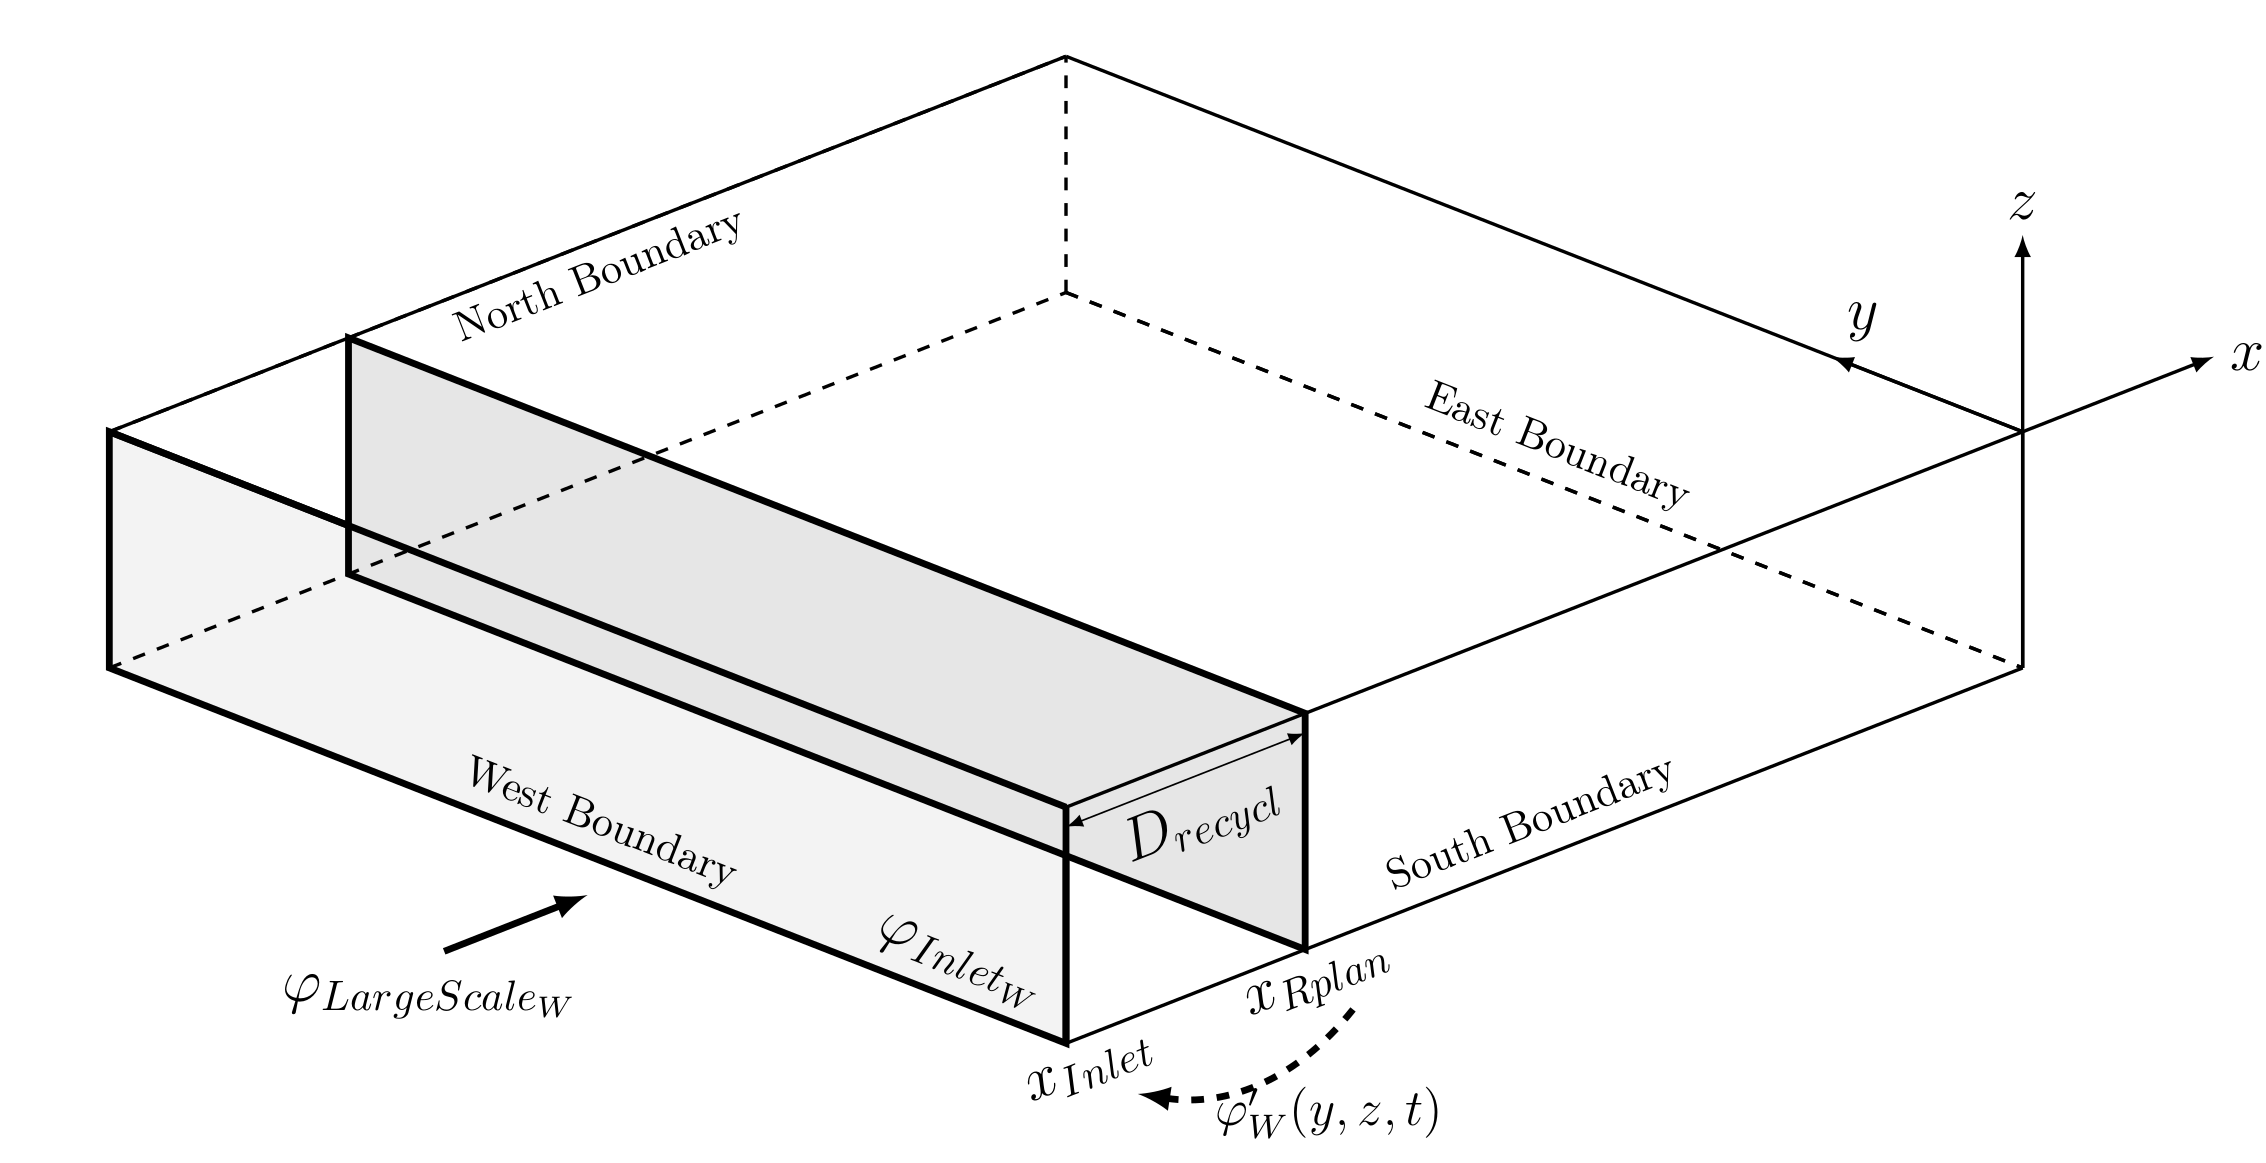
\includegraphics[width=1.\textwidth]{EPS/recycl3D_sketch.png}}
\caption{\label{recycling_sketch}\footnotesize \textit{Sketch of the turbulence recycling method used to generate turbulent inflow. For clarity, only the recycling of fluctuations at the West boundary is shown, but the same method applies on the four lateral sides.}}
\end{center}
\end{figure}

Figure \ref{recycling_sketch} shows a domain where inflow boundary conditions may be imposed at each lateral side (North, East, South, West). For the sake of clarity, the recycling method is only shown for the West boundary but the same method applies on the four lateral sides, a wind vector that is not aligned with the grid axis will thus be recycled on two sides. Considering the prognostic variable at the West boundary ($W$) $\varphi_W$ $\left(\varphi \in [u,v,w] \right)$,
the fluctuations $\varphi_W'$ are calculated in the recycling plane being located at a distance $D_{recycle}$ from the inlet. The fluctuations calculation reads:
\begin{equation}
\label{fluct}
\varphi_W'(y,z,t)  =  \varphi_W(x_{Rplan},y,z,t)-\overline{\varphi_W(x_{Rplan},y,z)},
\end{equation}
where $\varphi_W(x_{Rplan},y,z,t)$ is the instantaneous prognostic variable and $\overline{\varphi_W(x_{Rplan},y,z)}$ the time average of the prognostic variable in one point of the recycling plane.
\\The value of $\varphi_W'(y,z,t)$ is added to the corresponding inflow prognostic variable, $\varphi_{Inlet_W}$ :  
\begin{equation}
\label{InletField}
\varphi_{Inlet_W}(y,z,t)  =  \varphi_{LargeScale_W}(y,z,t)+\varphi_W'(y,z,t)\beta\psi_W(y,z,t),
\end{equation}
where $\varphi_{LargeScale_W}$ is the variable field imposed at the boundary, $\beta \in$ [0.1-0.3] a weighting coefficient preventing calculation divergence and $\psi_W(y,z,t)$ an inflow damping function calculated based on $T_{recycl}$ and the Brunt-V{\"a}is{\"a}l{\"a} period ($T_{BV}$): 
\begin{equation}
\label{dampingFunction}
\psi_w \rightarrow \left\{
    \begin{array}{ll}
        1 & \mbox{; if } T_{recycl}>4T_{BV} \\
        \frac{\displaystyle \left(T_{recycl}-2T_{BV} \right)}{\displaystyle \left(4T_{BV}-2T_{BV}\right)} & \mbox{; if } 2T_{BV} \leq T_{recycl} \leq 4T_{BV} \\
        0 & \mbox{; if } T_{recycl} < 2T_{BV}
    \end{array}
\right.  
\end{equation}
$\psi_W$ is calculated at the inlet, it is equal to 1 in neutral or near-neutral layers (e.g. in the boundary layer) and is linearly damped to 0 in stable layers. Its purpose is twofold: filtering the fluctuations due to gravity waves and preventing the imposed fluctuations to be affected by a potential increase in boundary-layer height between the recycling plane and the inlet.
\\Please note that even if the method has been built for grid-nested domains, it may also be applied to single domain configurations. Indeed, the variable field imposed at the boundary, $\varphi_{LargeScale_W}$, can result from any boundary condition type (father domain output or constant profile). However, in a single domain configuration, the efficiency of the method can not be assured. If the user is interested in using the recycling method for a single domain configuration only, she or he should adapt the recycling method. Some of the following ideas could be undertaken:
\begin{itemize}
 \item Introduce a strong initial perturbation in NAM\_PERT\_PRE (more likely a temperature perturbation)
 \item Recycle the fluctuations on a very short period, at least in a first run.
\end{itemize}
If none of the previous tips are working, it is suggested to perform a two-domain simulation. Having a coarse-resolution father domain almost not increases the computational cost and ensures the efficiency of the recycling method.
\\
\\Finally, please note that the turbulence recycling method has only been validated on idealized, cartesian, one-way nested and near-neutral cases.


%%%%%%%%%%%%%%%%%%%%%%%%%%%%%%%%%%%%%%%%%%%%%%%%%%%%%%%%%%%%%%%%%%%%%%%%%%%%%%

\section{References}
\decrefname
Bister, M., and K. A. Emanuel, 1998:
Dissipative heating and hurricane  intensity.
{\it Meteor. Atmos. Phys.}, {\bf 65}, 233-240.
\decrefname
Bougeault, P., and P. Lacarr\`ere, 1989:
Parameterization of orography-induced turbulence in a meso-beta scale model.
{\it Mon. Wea. Rev.}, {\bf 117}, 1872-1890.
\decrefname
Cuxart, J., 1997:
Planetary Boundary Layer Simulation: From LES to General Circulation Models,
Ph.D. thesis, European thesis - Barcelone.
\decrefname
Cuxart, J., P. Bougeault, and J.-L. Redelsperger, 2000:
A turbulence scheme allowing for mesoscale and large-eddy simulations.
{\it Quart. J. Roy. Meteor. Soc.}, {\bf 126}, 1-30.
\decrefname
Duynkerke, P.G., 1988:
Application of the E-$\epsilon$ turbulence closure model to the neutral
and stable atmospheric boundary layer.
{\it  J. Atmos. Sci.}, {\bf 45}, 865-880.
\decrefname
Emanuel K. A. 1994, Atmospheric convection, Chp8: Theory of mixing in cumulus cloud, p215
\decrefname
Hanjalic, K., and B. E. Launder, 1972:
A Reynolds stress model of turbulence and its application to thin shear flows.
{\it J. Fluid Mech.}, {\bf 52}, 609-638.
\decrefname
Honnert, R., Masson, V., Lac, C., and Nagel, T. 2021:
A Theoretical Analysis of Mixing Length for Atmospheric Models From Micro to Large Scales. 
{\it Front. Earth Sci}, {\bf 8}.
\decrefname
Klaassen, G. P., and T. L. Clark, 1985:
Dynamics of the cloud~environment interface and entrainment in small cumuli:
Two-dimensional simulations in the absence of ambient shear.
{\it  J. Atmos. Sci.}, {\bf 42}, 2621-2642.
\decrefname
Lemarié, F., Samson, G., Redelsperger, J. L., Giordani, H., Brivoal, T., and G. Madec, 2021:
A simplified atmospheric boundary layer model for an improved representation of air–sea interactions 
in eddying oceanic models: implementation and first evaluation in NEMO (4.0).
{\it Geoscientific Model Development}, {\bf 14(1)}, 543-572.
\decrefname
Lund, Thomas S and Wu Xiohua and Squires, Kyle D, 1998:
Generation of turbulent inflow data for spatially developing boundary layer simulations.
{\it Journal of Computational Physics}, {\bf 140}, 233-258.
\decrefname
Mu{\~n}oz-Esparza, D. and Kosovi{\'c}, B. and Mirocha, J. and van Beeck, J., 
 Bridging the Transition from Mesoscale to Microscale Turbulence in Numerical Weather Prediction Models.
{\it Boundary-Layer Meteorology}, {\bf 153}, 409-440.
\decrefname
Redelsperger, J.-L, and G. Sommeria, 1981:
M\'ethode de repr\'esentation de la turbulence d'\'echelle inf\'erieure
\`a la maille pour un mod\`ele tri-dimensionnel de convection nuageuse.
{\it  Boundary-Layer Meteor.}, {\bf 21(4)}, 509-530.
\decrefname
Rodier, Q., V. Masson, F. Couvreux and A. Paci, 2017: Evaluation of a Buoyancy and Shear Based Mixing Length for a Turbulence Scheme. {\it Frontiers in Earth Science}, {\bf 5}, 65.
\decrefname
Rodier Q, 2017. Param\'etrisation de la turbulence atmosph\'erique dans la couche limite stable. PhD manuscrit. Universit\'e Toulouse 3 Paul Sabatier (UT3 Paul Sabatier).
\decrefname
Skamarock, William C, 2004: Evaluating mesoscale NWP models using kinetic energy spectra.
{\it Monthly weather review}, {\bf 132}, 3019-3032.
\decrefname
Squire, P., 1958:
The spatial variation of liquid water and droplet concentration in cumuli.
{\it Tellus}, {\bf 10}, 372-380
\decrefname
Squire, P., 1958: Penetrative downdraughts in cumuli.
{\it Tellus}, {\bf 10}, 381-389
\decrefname
Tomas, S., and V. Masson, 2006: A parameterization of
third-order moments for the dry convective boundary layer. 
{\it Bound.-Layer. Meteor.}, {\bf 120}, 437-454.

\chapter{EDKF Shallow Convection Scheme}
\minitoc

%{\em by J. Pergaud}

\section{Introduction}

In a dry or cloudy convective boundary layer (CBL), the evolution of a variable $\phi$ is strongly influenced by vertical turbulent transport. Therefore, a good estimation of the second-order moment $\overline{w'\phi'}$ is needed to determine the tendency of $\overline\phi$ (the mean value of $\phi$) in the CBL.

Siebesma and Teixeira (2000) and Hourdin et~al. (2002) developed a new parameterization that combines eddy diffusivity and mass flux approaches in a consistent way. Organized strong updrafts are parameterized by the mass flux part while the remaining turbulence is parameterized using K-theory. This parameterization, named EDMF (Eddy-Diffusivity / Mass Flux), has been developed to model cloudy shallow convection and dry convection in a unified way. In the EDMF framework, the turbulent flux of a conservative variable $ \phi$ is defined as:
\begin{equation}
    \overline{w'\phi'}=-K\frac{\partial\overline{\phi}}{\partial{z}}+\frac{M_u}{\rho}(\phi_u-\overline{\phi}),
     \label{eq:EDMF}
\end{equation}
where $\rho$ is the density, $K$ is the turbulent diffusivity, $M_u$ is the convective mass flux $M_u=\rho a_u w_u$ ($a_u$ is the updraft grid fraction area and $w_u$ is the vertical velocity in the updraft), $\overline{\phi}$ is the mean value and $\phi_u$ is the updraft value of the variable $\phi$.

In this formulation, it is assumed that the size of the updraft area is very small compared to the grid size ($a_u \ll 1$), so the environmental field values are taken as the mean field values. The effect of downdrafts is neglected as this parameterization is used only for shallow convection. The eddy-diffusivity term represents the remaining fluctuations due to the non-organized small-scale local turbulence. 

Our parameterization contains an eddy-diffusivity term which is computed by the turbulence scheme of Cuxart et~al. (2000) and a mass flux term computed by an updraft scheme which is described in the following section. Due to the fact that we use the Kain-Fritsch scheme to diagnose entrainment and detrainment in the cloudy portion, we decided to call the new scheme EDKF for Eddy-Diffusivity / Kain-Fritsch.

\section{Description of the scheme}
\subsection{Updraft model}

The updraft model is defined as a single entraining/detraining rising parcel as in Soares et~al. (2004). One resulting updraft described by the mass flux is used to represent the effect of several plumes, and its characteristics are determined as a function of mixing between the updraft and its environment through entrainment $E$ (the inward mass flux from the environment to the updraft) and detrainment $D$ (the outward mass flux from the updraft to the environment). Moreover, the mass flux approximation assumes that the cloud ensemble is considered in steady state. The mass flux is defined as $M_u=\rho a_u w_u$, and its evolution is determined by a diagnostic equation of the mass continuity between the updraft and its surrounding environment (Fig. \ref{fig:SchemeDes}), 

\begin{eqnarray}
\frac{\partial{M_u}}{\partial{z}}=(E-D)\\
\mathrm{or,\hspace{5pt}}   \frac{1}{M_u}\frac{\partial{M_u}}{\partial{z}}=(\epsilon-\delta)
\label{eq:MFevol}
\end{eqnarray}
where $\epsilon$ and $\delta$ are respectively the entrainment rate  ($E=\epsilon M_u$) and the detrainment rate ($D=\delta M_u$).

\begin{figure} 
	\begin{center}
		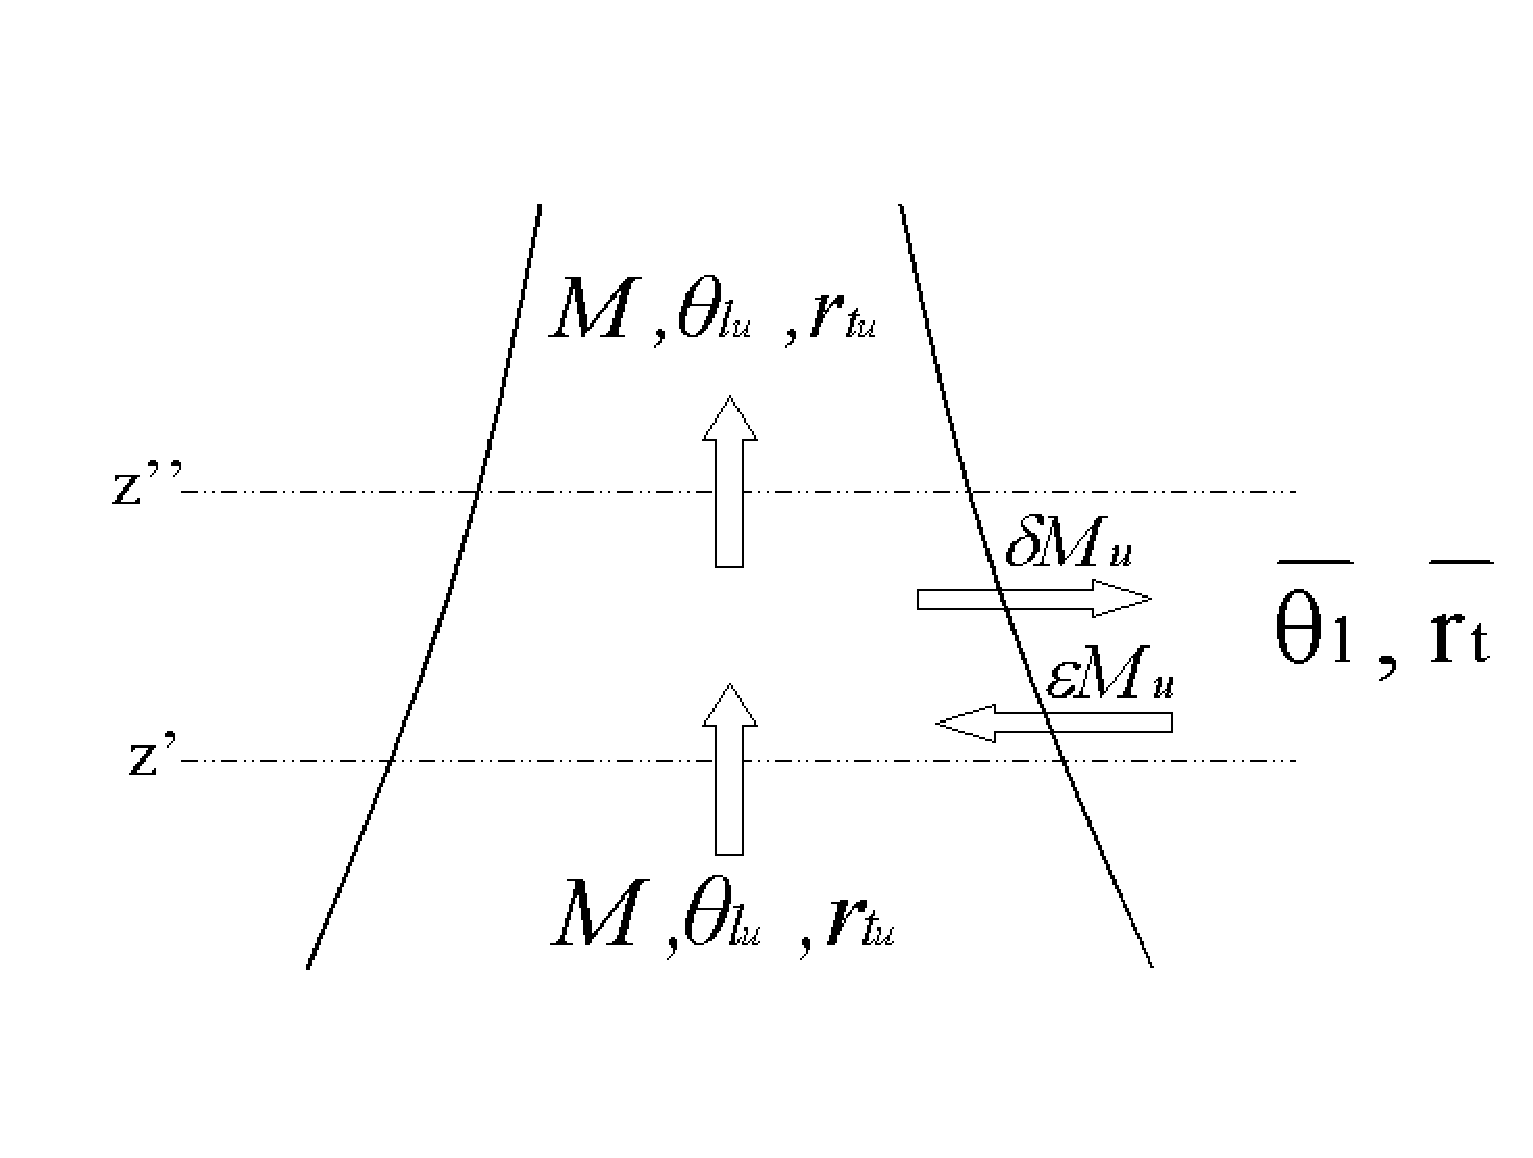
\includegraphics[width=7.5cm]{\EPSDIR/edkfscheme_v3.eps}
	\end{center}
	\caption{Variations of the updraft characteristics $M_u$, $\theta_{lu}$ and $r_{tu}$ and dependent on the mixing with the environment dictated by the entrainment $\epsilon M_u$ and the detrainment $\delta M_u$.}
	\label{fig:SchemeDes}
\end{figure}

The evolution of a conserved parcel characteristic $\phi_u$ during the ascent is defined as in Siebesma (1998):\\
\begin{equation}
\frac{\partial{M_u\phi_u}}{\partial{z}}=E\overline{\phi}-D\phi_u
\label{eq:Phievol1}
\end{equation}
using (\ref{eq:MFevol}) and simplified as:
\begin{equation}
\frac{\partial{\phi_u}}{\partial{z}}=-\epsilon(\phi_u-\overline{\phi})
\label{eq:Phievol2}
\end{equation}
where $\phi_u$ and $\overline{\phi}$ are respectively an updraft conserved variable and its mean value on the grid. This equation is used to determine the evolution of updraft conservative variables such as the liquid potential temperature $\theta_{lu}$ and the total mixing ratio $r_{tu}$ during ascent.

The vertical velocity ($w_u$) equation for the updraft is given by:
\begin{equation}
{w_u}\frac{\partial{w_u}}{\partial{z}}=B_u-\epsilon w_u^2 -P
\label{eq:WevolwithP}
\end{equation}
where on the right-hand side (rhs), the first term is the buoyancy, the second term is the entrainment, and
P represents the pressure term defined in, e.g. numerous studies (Simpson and Wiggert 1969; Siebesma et~al. 2003; Soares et~al. 2004) as a linear combination of the first two terms. Therefore, the equation is simplified as: 
\begin{equation}
w_u\frac{\partial{w_u}}{\partial{z}}=a B_u-b \epsilon w_u^2 
\label{eq:wevol1}
\end{equation}
where $a=1$ and $b=1$, defined respectively as a virtual mass coefficient and a drag coefficient (Simpson and Wiggert 1969). Numerical aspects are given in Appendix \ref{sec:annexe_w}. 

Using the definition of the mass flux, Soares et~al. (2004) and Siebesma et~al. (2007) were able to compute directly the mass flux in the dry portion of their updraft from the vertical velocity obtained from (\ref{eq:wevol1}) and using a constant fraction area. At cloud base, they used a constant value of the cloud fractional area to compute the mass flux and to close the scheme.

Equation (\ref{eq:wevol1}) is used to define the top of the updraft where $w_{u}$ vanishes but also to diagnose the updraft fraction area, $a_u$, which is not a constant or a closure of the scheme as in Soares et~al. (2004) and Siebesma et~al. (2007). 

Thanks to the independent computations of both mass flux $M_u$ (\ref{eq:MFevol}) and $w_{u}$ (\ref{eq:wevol1}), the updraft fraction area can vary vertically, and is defined as
\begin{equation}
   a_u=\frac{M_u}{\rho w_u}.
   \label{eq:updraft_fraction}
\end{equation}
The vertical variations of this last variable are important because $a_u$ is used to diagnose the cloud fraction (see next section).

The mass flux approach is also used to realize a non-local mixing of momentum along the vertical in addition to the mixing yet realized by the turbulent scheme via the eddy-diffusivity approach. But, since the momentum is not conservative, the effect of pressure perturbations is added using a parameterization from Gregory et~al. (1997). The evolution of the updraft horizontal wind component is defined as: 
%\begin{eqnarray}
\begin{equation}
    \frac{\partial{u_u}}{\partial{z}}=-\epsilon(u_u-\overline{u})+C_u\frac{\partial{\overline{u}}}{\partial{z}}\\
\label{eq:uevol},
\end{equation}
\begin{equation}
    \frac{\partial{v_u}}{\partial{z}}=-\epsilon(v_u-\overline{v})+C_v\frac{\partial{\overline{v}}}{\partial{z}}
\label{eq:uevol1},
\end{equation}
where $C_u=C_v=0.5$, and $u_u$ ($v_u$) represents the zonal (meridional) component of wind modified during the ascent in the updraft; $\overline{u}$ and $\overline{v}$ are zonal and meridional mean wind components respectively. 

\subsection{Lateral mass exchanges}

The definition of entrainment and detrainment is the crucial issue in this type of parameterization. Various studies have used different definitions for various PBL regimes (e.g., Siebesma 1998; Neggers et~al. 2002; De~Rooy and Siebesma 2008).

We have chosen to define lateral mass exchanges from physical characteristics of the CBL. Arakawa (2004) explained that buoyancy is an important parameter in shallow convection. Moreover, the vertical velocity $w_u$ is considered as a pertinent parameter in the description of mixing between dry updraft or the cloud and their environment in shallow convection. Neggers et~al. (2002) defined the entrainment as inversely proportional to vertical velocity for shallow cumulus convection, and Cheinet (2003) also applies this formulation to dry plumes. This means that $\epsilon$ is not constant but decreases with higher vertical velocities. In other terms, an updraft with strong vertical velocity will be isolated from its environment. 

In the dry portion of the CBL, $\epsilon$ and $\delta$ take into account physical characteristics of a buoyant ascending parcel. Equation (\ref{eq:wevol1}) shows that buoyancy is linked to vertical velocity, ${w_u}^2$ being a vertical integral of the buoyancy. However, locally, both can be independent, for example in the non-buoyant part where negative buoyant air can still be ascending. Young (1988) explained that the correlation between buoyancy and $w$ decreases in the upper part of the CBL, the buoyancy acting as a displacing force in the lower part of the CBL and as a restoring force in the upper part of the CBL. Thus, lateral mixing does not only depend on the vertical velocity as in Neggers et~al. (2002) but must be locally defined as an equilibrium between $w_u$ and buoyancy $B_u$. By dimensional analysis (Buckingham 1914), we obtain:
\begin{equation}
\epsilon_{dry},\delta_{dry} \propto \frac{B_u}{w_u^2} 
\label{eq:ent_delt_BW}
\end{equation}
where $B_u=g(\theta_{v,u}-\overline{\theta_v})/\overline{\theta_v}$ is the buoyancy of the air parcels in the updraft.

Near the ground, a relative strong buoyancy and a weak vertical velocity allow strong entrainment to import many air parcels in the updraft, implying a positive proportionality coefficient for $\epsilon$. Near the inversion, in the non-buoyant zone, much air is detrained implying a negative proportionality coefficient for $\delta$. Since entrainment and detrainment rates cannot be negative, the entrainment rate is zero where the updraft is non-buoyant compared to its surrounding environment. Conditional sampling of detrainment in LES has shown that detrainment is not null in the mixed layer (see Fig. 9c of Pergaud et~al. (2009)), so to keep a positive detrainment in the buoyant part of the updraft, a minimum detrainment is defined using a modified formulation from Lappen and Randall (2001): $\delta=(L_{up}-z)^{-1}$. 

Eventually, in the dry portion of the CBL, entrainment and detrainment are defined as:
\begin{eqnarray}
\epsilon_{dry} = Max\left[0,C_{\epsilon} \frac{B_u}{w_u^2} \right],  \\
\delta_{dry} = Max\left[\frac{1}{L_{up}-z}, C_{\delta} \frac{B_u}{w_u^2} \right],
\label{eq:eps_ent_delt}
\end{eqnarray}
where $L_{up}$ is the Bougeault and Lacarr\`ere (1989) (BL89) upward mixing length, $C_{\delta}$ and $C_{\epsilon}$ have been tuned to fit one-dimensional (1D) entrainment and detrainment to LES, $C_{\delta}=-10$ and $C_{\epsilon}=0.55$. Numerical aspects are given in Appendix \ref{sec:annexe_e}. 

In the cloudy part, several descriptions of the exchanges exist. 

We have chosen to define two different types of exchange differentiating the dry portion of the updraft from the moist one due to the fact that the environment of any updraft is strongly turbulent compared to the environment of a cloud. 
Taylor and Baker (1991) have emphasized the importance of buoyancy sorting in determining the cloud composition and in defining a continued lateral entrainment and detrainment. Zhao and Austin (2003) explained that a buoyancy sorting model can be used as a physically more realistic alternative to entraining plume models in shallow cumulus convection resolving notably the Warner paradox. In the parameterization presented here, if the lifting condensation level (LCL) is reached, lateral exchanges are computed using the parcel buoyancy sorting approach of Kain and Fritsch (1990) (KF90 in the following). Details are given in Kain and Fritsch (1990) and Bechtold et al. (2001) and you can see the chapter dealing with the Kain-Fritsch-Bechtold convection scheme.
However, minor modifications have been put in the EDKF parameterization, the new parameterization uses a uniform distribution of the air parcels although, in the original formulation, the distribution was Gaussian. 

\subsection{Scheme initialization and closure}

Since the scheme is integrated upward from the surface (level $z_{grd}$), $M_u(z_{grd})$ is computed as a function of $w_*$ as in Grant (2001) but at the surface, contrary to the closure at the cloud base defined by Grant (2001),
\begin{equation}
M_{u}(z_{grd})=C_{M_0}\rho(\frac{g}{\overline{\theta_{vref}}}\overline{{w'\theta_{v}'}_s} L_{up})^{1/3}
\label{eq:MFz0}
\end{equation}
where $\overline{{w'\theta_{v}'}_s}$ is the surface buoyancy flux, ${L_{up}}$ is the BL89 upward mixing length corresponding to the distance that a parcel leaving the ground travel due to buoyancy. The value of $C_{M_0}=0.065$ is based on LES results according to Pergaud et~al. (2009). Note that, in the surface layer, this value is larger than the value $C_{M_0}=0.03$ originally proposed by Grant (2001) at the LCL. 

The rising parcel characteristics are determined at the ground using the formulation of Soares et~al. (2004) in which an excess is added to the environmental values. For example, the updraft liquid potential temperature near the ground is:
\begin{equation}
\theta_{lu}(z_{grd})=\overline{\theta_l}(z_{grd})+\alpha\frac{{\overline{w'\theta_l'}}_s}{e^{1/2}(z_{grd})}
\label{eq:Phiz0}
\end{equation}
where the value of $\alpha$ is $0.3$ as in Soares et~al. (2004). Sensitivity tests in the range [0,1] indicate that results are independent of $\alpha$. This excess is formulated as a function of the surface-layer variability according to Troen and Mahrt (1986) who demonstrated that the excess is well correlated with the ratio of the surface heat flux and the square root of turbulent kinetic energy. A similar equation is used for $r_t$. 

At the surface, $w_u$ is initialized from the turbulent kinetic energy $e$ (provided by the turbulence scheme),
\begin{equation}
  {w_u}^2(z_{grd})=\frac{2}{3}e(z_{grd}).
  \label{Wz0}
\end{equation}

\subsection{The subgrid condensation scheme}

The updraft scheme represents the dynamical evolution of an air parcel during its ascent. Condensation can occur within the parcel. Therefore, a diagnostic sub-grid cloud based on the updraft characteristics is added. Although conservative variables are used, we can diagnose a sub-grid liquid mixing ratio $r_{c_{up}}$ and a cloud fraction $CF$. $r_{c_{up}}$ is computed from $\theta_l$, $r_t$ and pressure using a variation of all or nothing scheme since the updraft air parcels are considered completely cloudy.
$CF$ is defined proportional to the updraft fraction on the grid $a_u$:
\begin{equation}
  CF=C_{cf} * a_u
  \label{eq:CloudFrac}
\end{equation}
where $C_{cf}=2.5$. The horizontal size of the cloud is 2.5 times the size of the updraft. This parameter has been tuned to fit the 1D cloud fraction to LES results. This coefficient represents the difference between cloudy core fraction and cloud fraction.

The liquid mixing ratio can be approximated by the product between the cloud fraction previously computed and the updraft liquid mixing ratio computed from the updraft conservative variables (Bechtold and Cuijpers 1995):
\begin{equation}
  \overline{r_c}= CF * r_{c_{up}}
\label{eq:RcFrac}
\end{equation}

In our parameterization, $r_c$ is not a prognostic variable. If the mass flux becomes null, the cloud disappears totally. Only a prognostic cloud scheme can evaporate a cloud over several timesteps. So passive clouds that are not maintained by a thermal are not taken into account in the parameterization. However, here, $\overline{r_c}$ represents only the contribution of the shallow convection clouds. Others contributions for clouds can come from the subgrid turbulence scheme or from microphysics scheme (notably for resolved clouds). 

\section{Initialisation of Mass-Flux scheme at hectometric scales}

The triggering controls the activation of the mass-flux scheme at the surface while the closure controls its intensity. Often the boundary-layer mass-flux scheme triggers as soon as the surface sensible heat flux is positive while the intensity of the mass-flux at the ground is proportional to the convective velocity scale (see Pergaud et~al.,2009). 

Firstly, concerning the closure, Figure~\ref{trigDavid}a shows the subgrid mass-flux normalized by the convective velocity scale as a function of the normalized resolution in the IHOP case at $1200$ LT and the ARM case at $1400$ LT in the middle of the boundary layer. The mass-flux normalized by the convective velocity scale in both the IHOP and ARM cases is dependent on the resolution normalized by the height of the thermals : it is constant at mesoscales and larger than in LES. Here the mass flux is computed in the middle of the CBL. It cannot be diagnosed directly at the ground where there is no really thermal formed yet and where the turbulent is more strongly dependent on the subgrid turbulence scheme. The normalized mass flux as a function of the normalized resolution has the same shape at all altitudes in the boundary layer (not shown). Therefore, here we propose to make the constant of proportionality between the mass-flux at the ground and the convective velocity scale (computed at ground level for the whole domain, $w*$) dependent on the resolution by this function :

\begin{equation}
	\sigma(\frac{M_u}{w_*})=tanh(C\times\sqrt(\Delta x \times \Delta y)/L_{up})
\label{eq:MuHect}
\end{equation}
In the magenta fit plotted in Fig.~\ref{trigDavid}a, $C=1.83$. We propose to use this function in the parametrization in order to make it scale-aware.

Moreover, the subgrid mass-flux variability is larger in the grey zone than in the LES and at mesoscales. This is visible in Fig.~\ref{trigDavid}b which shows the standard deviation of the mass-flux normalized by the convective velocity scale ($\sigma(\frac{M_u}{w*})$) as a function of the normalized resolution in the IHOP case at $1200$~LT and the ARM case at $1400$~LT in the middle of the CBL. The large variability in the grey zone is also visible on the buoyancy and the entrainment (cf.~Honnert et al.,2016) and it is consistent with Dorrestijn et al. (2013) which showed that the heat flux variability is larger in the grey zone. The fit of the data of Fig.~\ref{trigDavid}b is:

\begin{figure}
\subfigure[\large Distribution]{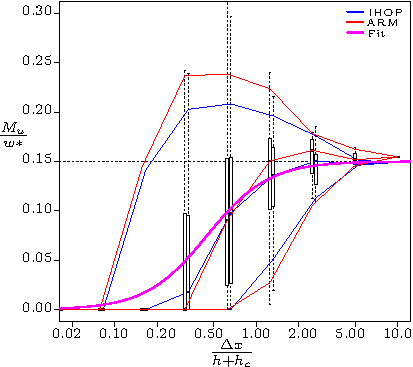
\includegraphics[width=0.45\textwidth]{EPS/MU_dx_fit_REVIEW}}
\subfigure[\large Dispersion]{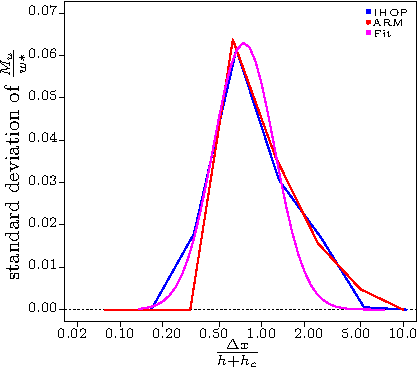
\includegraphics[width=0.45\textwidth]{EPS/dispersion_Mu_REVIEW}}
\caption[]{(a) Mass-flux of the subgrid thermals normalized by the convective velocity scale for grid cells ranging from $250$~m to $8$~km in the middle of the boundary layers of the ARM case at $1400$ LT (blue points) and the IHOP case at $1200$ LT (red points) as a function of $\Delta x/({h}+{h}_{c})$. Boxplots of the data (one per case) : the box shows 50\% of the data and the line 99.3\%. Median, quantile 5\% and 95\% in (red and blue) lines. A fit of the data (see text for more details) is in magenta. (b) Standard deviation of the same data in the same colors as in (a) as a function of the normalized horizontal resolution.}
\label{trigDavid}
\end{figure}

Concequently, the closure of the mass-flux scheme of Pergaud et~al. (2009) at hectometric scales depend on the model resolution following Eq.~\ref{eq:MuHect}.   

\section{Appendix}
\subsection{Mass flux in the surface layer compared to $w_*$}
\label{sec:MF_W}

The mass flux near the surface has been set proportional to the convective vertical velocity scale $w_*$ as in Grant (2001). The coefficient of proportionality $C_{M_0}$ in our scheme cannot have the same value than the one used by Grant (2001) due to the fact that Grant (2001) defines this relation at the LCL. So we used the CS defined in Pergaud et~al. (2009) to obtain mass flux values in the surface layer for different convective cases at different dates (IHOP, ARM).

\begin{figure}
 \begin{center}
		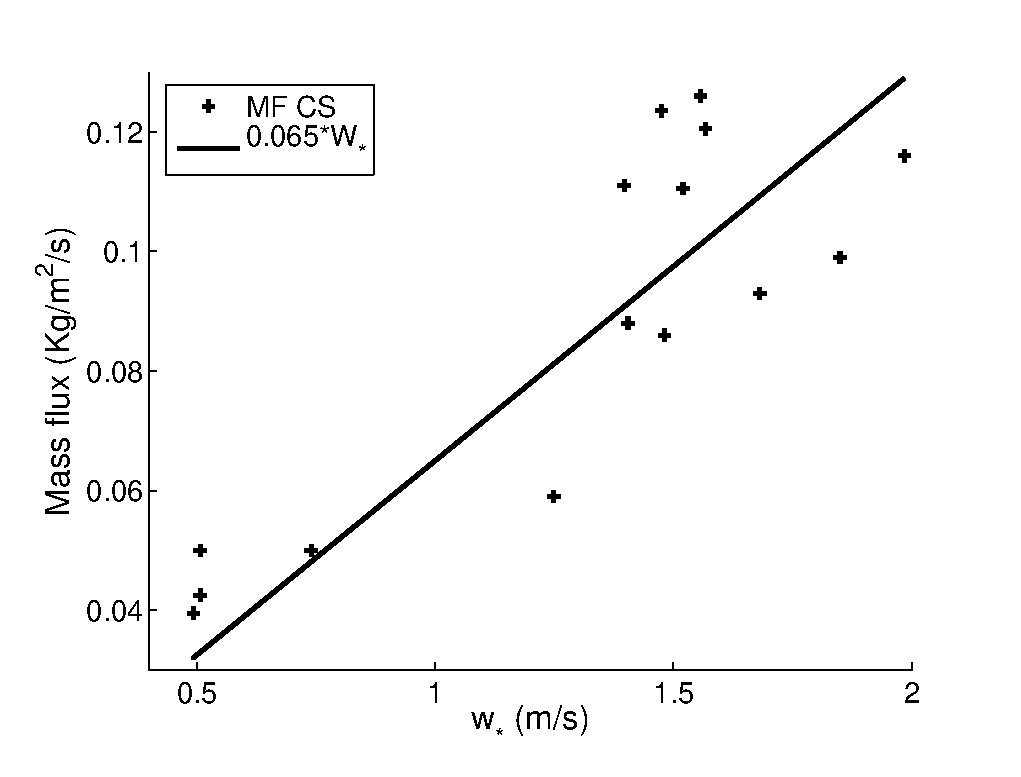
\includegraphics[width=9cm]{\EPSDIR/edkfMF_F_W.eps}
	\end{center}
	\caption{Mass flux in the surface layer computed using the Conditionnal Sampling defined in Pergaud et~al. (2009) versus sub-cloud layer velocity scale $w_*$. Line shows $M=0.065w_*$.}
	\label{fig:MF_F_W}
\end{figure}

Figure \ref{fig:MF_F_W} is a plot of the surface layer mass flux against sub-cloud layer velocity scale. The LES data suggest that $C_{M_0}=0.065$.

\subsection{Analytical solution for the vertical velocity $w_u$}
\label{sec:annexe_w}
Equation (\ref{eq:wevol1}) presents the computation for vertical velocity in the updraft $w_u$. Combining the equation for entrainment (\ref{eq:eps_ent_delt}), the $w_u$ equation becomes :
\begin{equation}
   \frac{\partial{{w_u}^2}} {\partial{z}}=2 a B_u-2 b C_{\epsilon}max(0,B_u)
\label{eq:wevol2}
\end{equation}
$C_{BUO}$ is defined equal to $2a$ if $B_u<0$ (entrainment is zero) and to $2(a-bC_{\epsilon})$ if $B_u>0$.
This equation is integrated over each layer. Figure \ref{fig:SchemeDes2} presents this integral. If $z'$ is layer bottom, $z''$ is layer top and $\Delta z_D = z''-z'$,  ${w_u}^2$ is defined by:

\begin{eqnarray}
   \int_{\Delta z_D}\frac{\partial{{w_u}^2}}{\partial{z}}dz=\int_{\Delta z_D} C_{BUO} B_u dz\\
   {w_u}^2(z'')-{w_u}^2(z')= C_{BUO}\frac{g}{\theta_{ref}}\int_{\Delta z_D} \left[    \theta_{v_{up}}(z)-\overline{\theta_v}(z)\right]  dz
   \label{eq:primitive1}
\end{eqnarray}

$\theta_{vup}$ is assumed constant between $z'$ and $z''$, and the variations of $\overline{\theta_v}$ is supposed linear between z' and z''.
\begin{eqnarray}
   \overline{\theta_v}(z)= \alpha_1 z + \overline{\theta_v}(z')\\
   \theta_{v_{up}}(z)    = \theta_{v_{up}}(z')
   \label{eq:fonction_lineaire}
\end{eqnarray}
So the integral for $w_u$ becomes
\begin{equation}
   {w_u}^2(z'') - {w_u}^2(z')= C_{BUO}\frac{g}{\theta_{ref}}\int_{\Delta z_D} \left[- \alpha_1z - \overline{\theta_v}(z') + \theta_{v_{up}}(z')\right]  dz \\
   \label{eq:primitive2}
\end{equation}

After computation, $w_u$ at the level $z''$ computed from the level $z'$ is :
\begin{equation}
   {w_u}^2(z'')= C_{BUO}\frac{g}{\theta_{ref}} \Delta z_D(\frac{ - \alpha_1}{2}\Delta z_D - \overline{\theta_v}(z') + \theta_{v_{up}}(z')) + {w_u}^2(z') 
   \label{eq:primitive3}
\end{equation}


\subsection{Analytical integrated solution for entrainment and detrainment}
\label{sec:annexe_e}

The entrainment $\epsilon$ is defined by equation (\ref{eq:eps_ent_delt}). This equation is integrated, as for $w_u$, on each vertical grid size for example between $z'$ and $z''$ (see on Fig. \ref{fig:SchemeDes2}):
\begin{equation}
   \epsilon = \frac{C_{\epsilon}}{\Delta z_D}\int_{\Delta z_D} \frac{B}{{w_u}^2}dz\\
   \label{eq:primitive4}
\end{equation}
Using (\ref{eq:primitive3}), $\epsilon$ becomes
\begin{eqnarray}
   \epsilon = \frac{C_{\epsilon}g}{\Delta z_D \theta_{ref}}\int_{\Delta z_D} \frac{ \theta_{v_{up}}(z') - \alpha_1 z +  \overline{\theta_v}(z')} {C_{BUO}\frac{g}{\theta_{ref}} z( - \alpha_1 z - \overline{\theta_v}(z') + \theta_{v_{up}}(z')) + {w_u}^2(z')}dz\\
   \epsilon = \frac{C_{\epsilon}}{\Delta z_D C_{BUO}}\int_{\Delta z_D} \frac{- \alpha_1 z + \theta_{v_{up}}(z') +  \overline{\theta_v}(z')} { \frac{- \alpha_1}{2}z^2 - \overline{\theta_v}(z')z + \theta_{v_{up}}(z')z) + \frac{\theta_{ref} {w_u}^2(z')} {g C_{BUO}}}dz.
   \label{eq:primitive5}
\end{eqnarray}

noting $X=\frac{- \alpha_1}{2}z^2 - \overline{\theta_v}(z')z + \theta_{v_{up}}(z')z) + \frac{\theta_{ref}{w_u}^2(z')}{gC_{BUO}}$:

\begin{eqnarray}
   dX= ((- \alpha_1) z + \theta_{v_{up}}(z') +  \overline{\theta_v}(z'))dz\\
   \epsilon = \frac{C_{\epsilon}}{C_{BUO}\Delta z_D}\int_{\Delta z_D} \frac{dX}{X}\\
   \epsilon = \frac{C_{\epsilon}}{C_{BUO}\Delta z_D}[Ln(X)]_{\Delta z_D}
   \label{eq:primitive6}
\end{eqnarray}

After computation, $\epsilon$ is defined as :
\begin{equation}
   \epsilon=\frac{C_{\epsilon}}{C_{BUO}\Delta z_D} ln\left[ 1+\frac{C_{BUO}\Delta z_D}{{w_u}^2(z')\theta_{ref}} (\frac{- \alpha_1}{2} \Delta z - \theta_{v_{up}}(z') +  \overline{\theta_v}(z'))\right]\\
   \label{eq:epsilon}
\end{equation}
where $\alpha_1$ is defined as previously. An identical solution can be found for $\delta$ taking the absolute value of the buoyancy.

A formulation of the transition between cloudy and dry regime is added to limit the sensitivity of the scheme to the change in the computation of entrainment and detrainment. If a liquid mixing ratio is detected at z'' using an "all or nothing" adjustment from updraft variables, the LCL height is determined assuming a linear increase of $r_c$ with height. A weight for the KF90 lateral exchanges is defined proportional to the cloudy part occupying grid and integral dry entrainment and detrainment are computed only on the height of the dry part.

\begin{figure}
  \begin{center}
    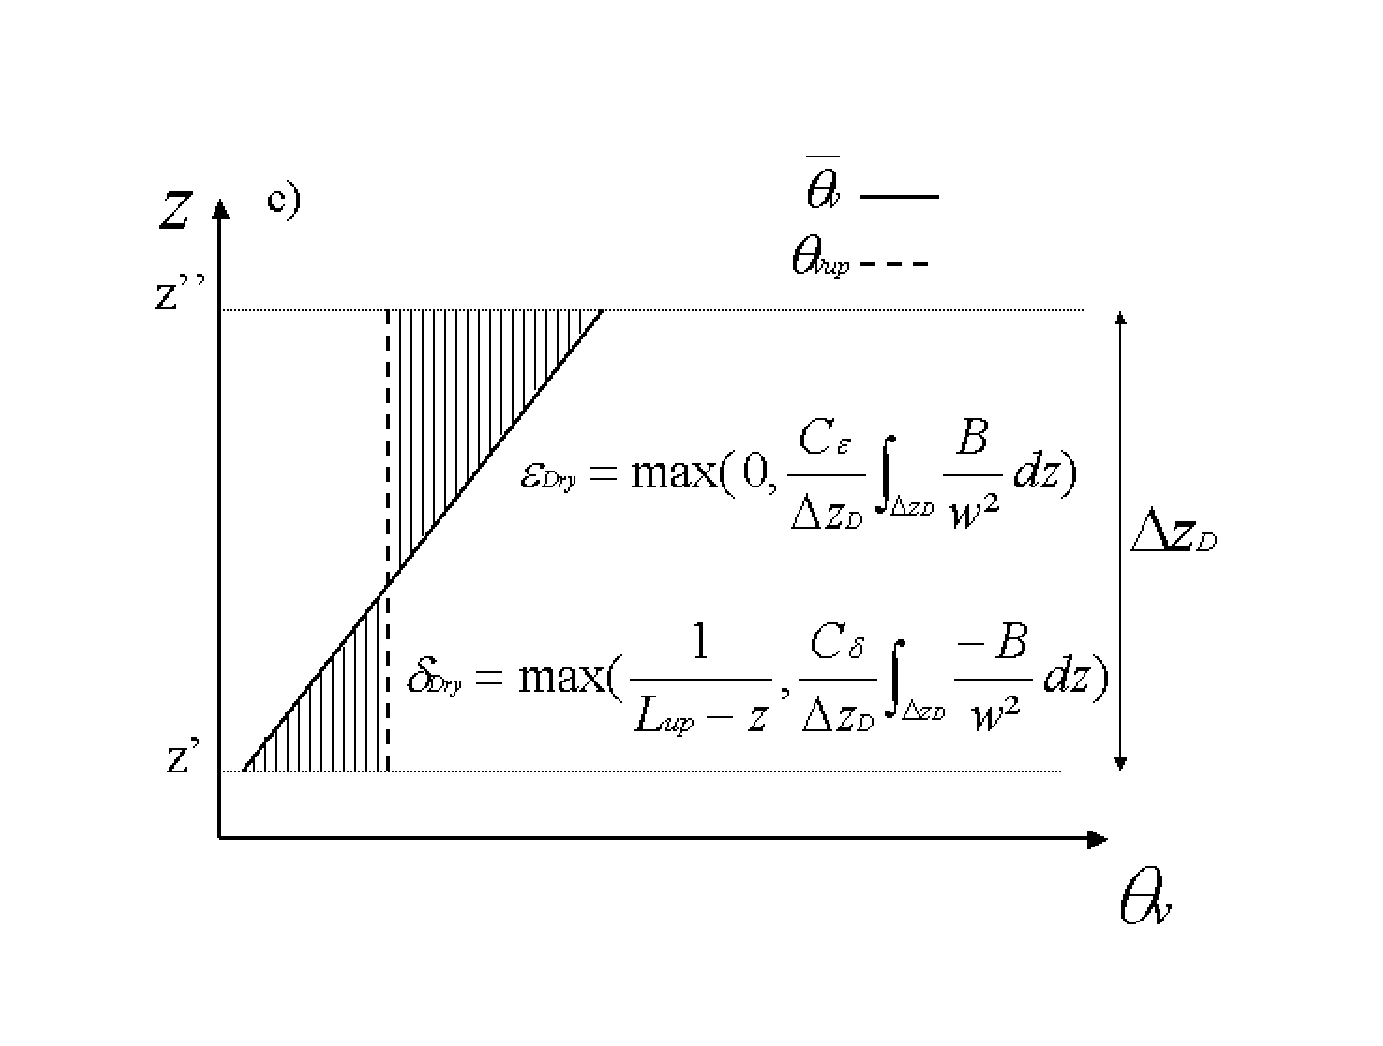
\includegraphics[width=11cm]{\EPSDIR/edkfTHL_DRY_PWT_v2.eps}
  \end{center}
  \caption{Parameterized entrainment and detrainment for dry layer}
  \label{fig:SchemeDes2}
\end{figure}

\section{References}

\noindent \por
Arakawa, A., 2004: 
The Cumulus Parameterization Problem: Past, Present, and Future.
{\it J. Clim.}, {\bf 17}, 2493--2525.

\noindent \por
Bechtold, P., and~ J. W. M. Cuijpers, 1995:
Cloud perturbations of temperature and humidity: A LES study.
{\it Bound. Layer. Meteor.}, {\bf 76}, 377--386.

\noindent \por
Bechtold, P., E. Bazile, P. Mascart and E. Richard, 2001:
A Mass flux convection scheme for regional and global models.
{\it Quart. J. Roy. Meteor. Soc.}, {\bf 127}, 869-886.

\noindent \por
Bougeault, P, and P. Lacarr\`ere, 1989: Parameterization of Orography-Induced
  Turbulence in a Mesobeta-Scale Model.
{\it Mon. Wea. Rev.}, {\bf 117}, 1872--1890.

\noindent \por
Buckingham, E., 1914: On physically similar systems: Illustrations of the use of
  dimensional equations.
{\it Phys. Rev.}, {\bf IV}, 345--376.

\noindent \por
Cheinet, S., 2003: A multiple Mass-Flux Parameterization for the
  Surface-Generated Convection. Part1: Dry Plumes.
{\it J. Atmos. Sci.}, {\bf 60}, 2313--2327.

\noindent \por
Cuxart, J., P. Bougeault, and J.-L. Redelsperger, 2000:
A turbulence scheme allowing for mesoscale and large-eddy simulations.
{\it Quart. J. Roy. Meteor. Soc.}, {\bf 126,} 1--30.

\noindent \por
De~Rooy, W. C., and P. Siebesma, 2008:
 A simple parameterization for detrainment in shallow cumulus.
{\it Mon. Wea. Rev.}, {\bf 136}, 560--576.

\noindent \por
Dorrestijn J, Crommelin DT, Siebesma AP and Jonker HJJ, 2013:
Stochastic convection parametrization estimated from high-resolution model data.  27:133--148
{\it Theor Comput Fluid Dyn}, {\bf 27}, 133--148.

\noindent \por
Grant, A. L. M., 2001: Cloud-base fluxes in the cumulus-capped boundary layer.
{\it Quart. J. Roy. Meteor. Soc.}, {\bf 127}, 407--421.

\noindent \por
Gregory, D., R. Kershaw, and P. M. Inness, 1997:
 Parametrization of momentum transport by
  convection. II: Tests in single-column and general circulation models.
{\it Quart. J. Roy. Meteor. Soc.}, {\bf 123}, 1153--1183.

\noindent \por
Honnert, R., Couvreux, F., Masson, V. et David Lancz, 2016 :
Sampling the Structure of Convective Turbulence and Implications for Grey-Zone Parametrizations
{\it Bound. Layer. Meteor.}, {\bf 160}, 133.

\noindent \por
Hourdin, F., F. Couvreux, and L. Menut, 2002:
 Parameterization of the Dry Convective
  Boundary Layer Based on a Mass Flux Representation of Thermals.
{\it J. Atmos. Sci.}, {\bf 59}, 1105--1122.

\noindent \por
Kain, J. S., and J. M. Fritsch, 1990: A one-dimensional
entraining/detraining plume model and its application in
convective parameterizations. {\it J. Atmos. Sci.},
{\bf 47}, 2784-2802.

\noindent \por
Lappen, C. L., and D. A. Randall, 2001:
Toward a Unified Parameterization of the Boundary Layer and Moist Convection. 
Part2 : Lateral Mass Exchanges and Subplume-Scale Fluxes.
{\it J. Atmos. Sci.}, {\bf 58}, 2037--2051.

\noindent \por
Neggers, R. A. J., P. Siebesma, and H. J. J. Jonker, 2002:
 A Multiparcel Model for Shallow Cumulus Convection.
{\it J. Atmos. Sci.}, {\bf 59}, 1655--1668.

\noindent \por
Pergaud, J., V. Masson, S. Malardel, and F. Couvreux, 2009:
A Parameterization of Dry
  Thermals and Shallow Cumuli for Mesoscale Numerical Weather Prediction.
{\it Bound. Layer. Meteor.}, {\bf 132}, 83--106.

\noindent \por
Siebesma, P., 1998: Shallow Cumulus Convection.
In {\it "Buoyant convection in geophysical flows"} (Eds. E.J. Plate et al),
441--486.

\noindent \por
Siebesma, P., C. S. Bretherton, A. Brown, A. Chlond, J. Cuxart, 
P. G. Duynkerke, H. Jiang, M. Khairoutdinov, D. Lewellen, C. H. Moeng,
E. Sanchez, B. Stevens, and D. E. Stevens, 2003:
A Large Eddy Simulation Intercomparaison Study of Shallow Cumulus Convection.
{\it J. Atmos. Sci.}, {\bf 60}, 1201--1219.

\noindent \por
Siebesma, P., P. M. M. Soares, and J. Teixeira, 2007:
A combined Eddy-Diffusivity Mass-Flux 
approach for the convective boundary layer.
{\it J. Atmos. Sci.}, {\bf 64}, 1230--1248.

\noindent \por
Simpson J, and V. Wiggert, 1969: Models of precipitating cumulus towers.
{\it Mon. Wea. Rev.}, {\bf 97}, 471--489.

\noindent \por
Soares, P. M. M., P. M. A. Miranda, A. P. Siebesma, and J. Teixeira, 2004:
An Eddy-Diffusivity/Mass-Flux parameterization for dry and shallow cumulus
  convection.
{\it Quart. J. Roy. Meteor. Soc.}, {\bf 130}, 3055--3079.

\noindent \por
Taylor, G. R., and M. B. Baker, 1991: 
Entrainment and Detrainment in cumulus clouds.
{\it J. Atmos. Sci.}, {\bf 48}, 112--121.

\noindent \por
Troen, I. B., and L. Mahrt, 1986:
A simple model of the atmospheric boundary layer: 
Sensitivity to surface evaporation.
{\it Bound. Layer. Meteor}, {\bf 37}, 129--148.

\noindent \por
Young, G. S., 1988: Turbulence Structure of the convective Boundary Layer. Part II:
  Phoenix 78 Aircraft Observations of Thermals and their environment.
{\it J. Atmos. Sci.}, {\bf 45}, 727--735.

\noindent \por
Zhao, M., and P. H. Austin, 2003:
Episodic Mixing and Buoyancy-Sorting Representations
  of Shallow Convection: A Diagnostic Study.
{\it J. Atmos. Sci.}, {\bf 60}, 892--912.

\chapter{HRIO Shallow Convection Scheme}
\minitoc

%{\em by R. Honnert}

\section{Introduction}

The grey zone of turbulence is defined by Wyngaard (2004) as the scales on the order of the energy-containing turbulence scale. At these resolutions, the turbulence structures are neither entirely subgrid scale (as in global and mesoscale models) nor largely resolved (as in large-eddy simulations (LES)). Honnert et al. (2011) used LES coarse-graining to produce similarity functions linking the subgrid or resolved part of the turbulent fluxes and the horizontal resolution of the model out of the height of the thermals. They indicated that the grey zone exists from resolutions smaller than two times the boundary-layer height in convective boundary layers (CBL). Regional models are now approaching the sub-kilometic scales and Honnert et al. (2011) showed that neither unidirectional (1D) non-local mesoscale boundary-layer (BL) turbulence scheme nor isotropic (3D) LES schemes are appropriate at these scales. That is why the turbulence schemes have to be adapted to the grey zone of turbulence. 

Boutle et al. (2014) blended a 3D-Smagorinsky with a 1D non-local BL scheme with the help of the similarity functions proposed by Honnert et al. (2011). Ito et al. (2015) extended the Mellor and Yamada scheme by modifiing the length scales using statistics obtained from LES coarse-graining. Shin and Hong (2015) quantified the local and non-local turbulence at scales in the grey zone to adjust the vertical profiles resulting from their non-local K-gradient scheme.  

These adaptations stongly depend on the schemes which are currently used at mesoscale or LES. At M\'et\'eo-France, the turbulence in the atmospheric BL is represented by an eddy-diffusivity/mass-flux  parametrization (EDMF - Hourdin et al. (2002), Soares et al. (2004)). The updraughts are represented by the mass-flux scheme which starts at the ground (hereafter PM09 - Pergaud et~al., 2009 ) and represents the shallow convection, while the rest of the turbulence is represented by a K-gradient scheme (hereafter CBR - Cuxart et~al., 2000)). Both parts of this scheme are being modified to adapt M\'et\'eo-France models to the grey zone of turbulence.   
In this article, modifications of PM09 are presented in the second section as well as preliminary results in the third section. As perspective, the "true" CBR mixing lengths in the grey zone are presented.

\section{Description of the scheme}

As many mass-flux schemes, PM09 is based on several assumptions which are valid at large scales. It assumes in particular that the thermal surface is small, the resolved vertical velocity is zero, and the thermal field is quasi-stationnary. 

Honnert at al. (2016) determined the characteristics of the non-local turbulence (BL thermals) in the grey zone by means of a conditional sampling. Figure~\ref{f01} shows a $16$-km long horizontal cross-section of an LES. The thermals (in white) and the part of the thermals which impact the subgrid mass-flux scheme at $1$-km resolution (in black) have been determined by the conditional sampling of Honnert at al. (2016). The environment of the structures is in red. Figure~\ref{f01} shows that at $16$-km resolution, PM09's assumptions are valid : the thermal surface is small, the resolved vertical velocity is zero, as the grid-cell contains both the updraughts and the compensatory subsidence, and the thermal field is quasi-stationnary. However, in the grey-zone, they are not verified. Indeed, as seen on the $1$-km zoom of Fig.~\ref{f01}, the thermal surface (in black) may be large, the resolved vertical velocity is not zero, as one thermal can fill the grid-cell, and the thermal field is probably not quasi-stationnary.   
\begin{figure}[h!]
	\centering
	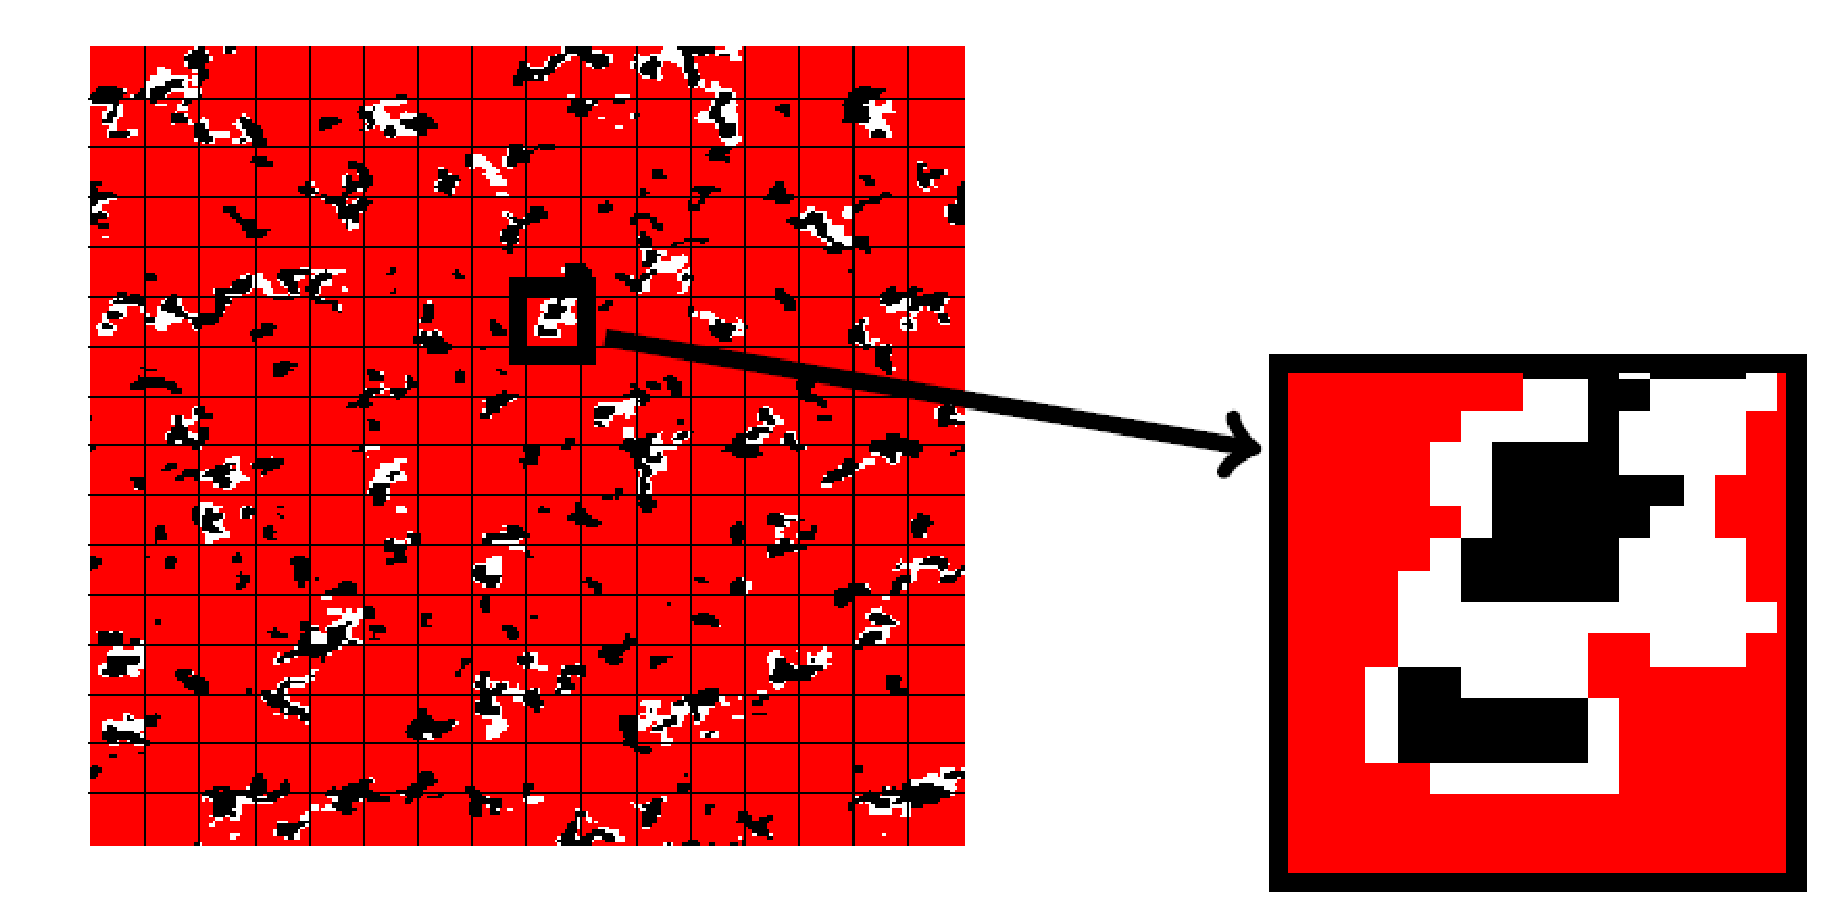
\includegraphics[width=0.8\textwidth]{EPS/f01}
	\caption{\label{f01}$16$-km long horizontal cross-section of an LES (IHOP case , 1400 LT, $500$-m altitude) and $1$-km long zoom. The thermal fraction is in white, the core of the thermals (strong vertical velocity) is in black and the environment is in red. See Honnert et al. (2016)}
\end{figure}

However, mass-flux schemes can be developed without the three assumptions presented before. The initial schemes (PM09, Rio et al. 2009) describe the behaviour of parameters of one unique thermal in the mesh (the vertical velocity $w_u$, the mass-flux $M_u$, the total potential temperature ${\theta_l}_u$, the thermal surface area $\alpha$, the buoyancy inside the thermal $B_u$ and the pressure and the entrainment ($\epsilon$)/ detrainment ($\delta$) lateral closure). $a_1$ and $b_1$ are constant. 
Eq.~(1-4) show the modifications (in red) of PM09. The non-negligible resolved vertical velocity ($\overline{w}^{\Delta x}$) is added in Eq.~(1,3-4). The thermal surface is not negligible and appears at the denominator in Eq.~(3-4). The surface triggering of the mass-flux (${M_u}_{z=0}$, Eq.~(5)) depends on the resolution.  

\begin{eqnarray}
	M_u&=&\rho\alpha(w_u\color{red}{-\overline{w}^{\Delta x}}\color{black}{)}\\
	\frac{1}{M_u}\frac{\partial M_u}{\partial z}&=&\epsilon-\delta\\
	\frac{\partial {\theta_l}_u}{\partial z}&=&-\frac{\color{red}{\epsilon}}{\color{red}{1-\alpha}}({\theta_l}_u -\overline{\theta_l}^{\Delta x})\\
	\frac{1}{2}\frac{\partial (w_u\color{red}{-\overline{w}^{\Delta x}\color{black}{)}^2}\color{black}{)}}{\partial z}&=&a_1B_u-b_1\frac{\color{red}{\epsilon}}{\color{red}{1-\alpha}}(w_u\color{red}{-\overline{w}^{\Delta x}}\color{black}{)^2}\\
\end{eqnarray}

Then, the finer the resolution or the smaller the BL height, the smaller the subgrid turbulent flux. The scheme produces less subgrid turbulence. Consequently, resolved BL thermals are created.

\section{Initialisation of Mass-Flux scheme}


he triggering controls the activation of the mass-flux scheme at the surface while the closure controls its intensity. Often the boundary-layer mass-flux scheme triggers as soon as the surface sensible heat flux is positive while the intensity of the mass-flux at the ground is proportional to the convective velocity scale (see Pergaud et~al.,2009). 

Firstly, concerning the closure, Figure~\ref{trigDavid}a shows the subgrid mass-flux normalized by the convective velocity scale as a function of the normalized resolution in the IHOP case at $1200$ LT and the ARM case at $1400$ LT in the middle of the boundary layer. The mass-flux normalized by the convective velocity scale in both the IHOP and ARM cases is dependent on the resolution normalized by the height of the thermals : it is constant at mesoscales and larger than in LES. Here the mass flux is computed in the middle of the CBL. It cannot be diagnosed directly at the ground where there is no really thermal formed yet and where the turbulent is more strongly dependent on the subgrid turbulence scheme. The normalized mass flux as a function of the normalized resolution has the same shape at all altitudes in the boundary layer (not shown). Therefore, here we propose to make the constant of proportionality between the mass-flux at the ground and the convective velocity scale (computed at ground level for the whole domain, $w*$) dependent on the resolution by this function :

\begin{equation}
	\sigma(\frac{M_u}{w_*})=tanh(C\times\sqrt(\Delta x \times \Delta y)/L_{up})
\label{eq:MuHect}
\end{equation}
In the magenta fit plotted in Fig.~\ref{trigDavid}a, $C=1.83$. We propose to use this function in the parametrization in order to make it scale-aware.

Moreover, the subgrid mass-flux variability is larger in the grey zone than in the LES and at mesoscales. This is visible in Fig.~\ref{trigDavid}b which shows the standard deviation of the mass-flux normalized by the convective velocity scale ($\sigma(\frac{M_u}{w*})$) as a function of the normalized resolution in the IHOP case at $1200$~LT and the ARM case at $1400$~LT in the middle of the CBL. The large variability in the grey zone is also visible on the buoyancy and the entrainment (cf.~Honnert et al., 2016) and it is consistent with Dorrestijn et al. (2013) which showed that the heat flux variability is larger in the grey zone. The fit of the data of Fig.~\ref{trigDavid}b is:

Concequently, the closure of the mass-flux scheme of Pergaud et~al. (2009) at hectometric scales depend on the model resolution following Eq.~\ref{eq:MuHect}.

\section{References}

\noindent \por
Boutle, I. A., Eyre, J. E. J., and Lock, A. P., 2014:
Seamless stratocumulus simulation across the turbulent grey zone. 
{\it Mon. Wea. Rev.}, {\bf 42}, 1655--1668. 

\noindent \por
Cuxart, J., P. Bougeault, and J.-L. Redelsperger, 2000:
A turbulence scheme allowing for mesoscale and large-eddy simulations.
{\it Quart. J. Roy. Meteor. Soc.}, {\bf 126,} 1--30.

\noindent \por
Dorrestijn J, Crommelin DT, Siebesma AP and Jonker HJJ, 2013:
Stochastic convection parametrization estimated from high-resolution model data.  27:133--148
{\it Theor Comput Fluid Dyn}, {\bf 27}, 133--148.

\noindent \por
Honnert, R., Masson, V., and Couvreux, F., 2011:
A diagnostic for evaluating the representation of turbulence in atmospheric models at the kilometric scale.  
{\it J. Atmos. Sci.}, {\bf 68(12)}, 3112--3131.

\noindent \por
Honnert, R., Couvreux, F., Masson, V., and David Lancz, 2016 :
Sampling the Structure of Convective Turbulence and Implications for Grey-Zone Parametrizations
{\it Bound. Layer. Meteor.}, {\bf 160}, 133.

\noindent \por
Hourdin, F., F. Couvreux, and L. Menut, 2002:
Parameterization of the Dry Convective Boundary Layer Based on a Mass Flux Representation of Thermals.
{\it J. Atmos. Sci.}, {\bf 59}, 1105--1122.

\noindent \por
Ito, J., Niino, H., Nakanishi, M., and Moeng, C. H., 2015:
An extension of the Mellor–Yamada model to the terra incognita zone for dry convective mixed layers in the free convection regime.
{\it Bound. Layer. Meteor.}, {\bf 157(1)}, 23--43.

\noindent \por
Pergaud, J., V. Masson, S. Malardel, and F. Couvreux, 2009:
A Parameterization of Dry
  Thermals and Shallow Cumuli for Mesoscale Numerical Weather Prediction.
{\it Bound. Layer. Meteor.}, {\bf 132}, 83--106.

\noindent \por
Rio, C., F. Hourdin, J. Y. Grandpeix, and J. P. Lafore, 2009:
Shifting the diurnal cycle of parameterized deep convection over land.
{\it Geophysical Research Letters.}, {\bf 36}, 7.

\noindent \por
Shin, H., and Hong, S., 2013 : 
Analysis on resolved and parametrized vertical transports in the convective boundary layers at the gray-zone resolution. 
{\it J. Atmos. Sci.}, {\bf 70}, 3248--3261.

\noindent \por
Soares, P. M. M., P. M. A. Miranda, A. P. Siebesma, and J. Teixeira, 2004:
An Eddy-Diffusivity/Mass-Flux parameterization for dry and shallow cumulus
  convection.
{\it Quart. J. Roy. Meteor. Soc.}, {\bf 130}, 3055--3079.

\noindent \por
Wyngaard JC, 2004 : 
Toward numerical modelling in the ‘Terra Incognita’. J Atmos Sci 61:1816–1826
{\it J. Atmos. Sci.}, {\bf 61}, 1816--1826.

%%%%%%%%%%%%%%%%%%%%%%%%%%%%%%%%%%%%%%%%%%%%%%%%%%%%%%%%%%%%%%%%%%%%%%%%%%%%%%
% CONTRIBUTION TO THE MESONH BOOK1: "Convection Scheme"
% Author : Peter Bechtold
% Original : October 10, 1997
% Update   : Mai 21, 2002
%%%%%%%%%%%%%%%%%%%%%%%%%%%%%%%%%%%%%%%%%%%%%%%%%%%%%%%%%%%%%%%%%%%%%%%%%%%%%%
%
%
% DEFINITIONS:
%
% Repertoire localisant les fichiers de figure
%\documentclass[12pt]{book}
%%%%%%%%%%%%%%%%%%%%%%%%%%%%%%%%%%%%%%%%%%%%%%%%%%%%%%%%%%%
%\include{../mnh_macros.tex}
%\setcounter{page}{1}
%%%%%%%%%%%%%%%%%%%%%%%%%%%%%%%%%%%%%%%%%%%%%%%%%%%%%%%%%%%
% Repertoire localisant certains fichiers de figure
%\def\EPSDIR {eps}
%%%%%%%%%%%%%%%%%%%%%%%%%%%%%%%%%%%%%%%%%%%%%%%%%%%%%%%%%%%
%
%\begin{document}
\chapter{Convection Scheme}
\minitoc
\section{Introduction}

It has been  well recognized since the 1960s (e.g.
Charney and Eliassen 1964; Manabe and Strickler 1964; Kuo 1965;
Ooyama 1971; Yanai et al. 1973) that cumulus convection
is one of the major processes that affects the dynamics and energetics
of  atmospheric circulation systems.
Since then many cumulus parameterization schemes
 have been developed for numerical weather prediction (NWP) models and
General Circulation Models (GCMs), to account for
the subgrid-scale release of latent heat and mass transport associated
with convective clouds. A non-exhaustive list of these schemes includes e.g.
Arakawa and Schubert (1974), Anthes (1977), Kuo and Raymond (1980),
Fritsch and Chappell (1980),
Bougeault (1985), Betts and Miller (1986),
Tiedtke (1989), Gregory and Rowntree (1990), Kain and Fritsch (1990),
Emanuel (1991), Donner (1993), Grell (1993),
Wang and Randall (1996), Sun and Haines (1996), and Hu (1997).
The common point of all cumulus parameterizations is that they aim to diagnose the
presence of larger-scale conditions that would support the development of
convective activity and, under appropriate conditions, to introduce tendencies
for temperature and moisture (and possibly momentum) that would be consistent
with the effects of convective activity.  In particular, most parameterizations are
designed to drive the model atmosphere towards a convectively adjusted state
when they activate.  This adjusted state is either predefined ("adjustment"
schemes) or is computed using a bulk or spectral cloud model
and adjusting the atmosphere through mass exchange between the cloud
and the environment (mass flux schemes).

Two necessary characteristics of any convective parameterization are i) a
reasonable set of criteria to determine when convective adjustment should be
initiated, and ii) reasonable procedures for determining the characteristics of
a final convectively-adjusted state.
 In fully
prognostic dynamic models, the efficacy of a convection parameterization is
often measured by factors such as  i)  does it activate at the right time and
place?  ii)  does it produce the right amount and areal coverage of
precipitation?  and iii)  does it enhance the predictive skill of
its host model?
Of course, there are many ways of evaluating these measures, and the third
criteria above, in particular, depends on the needs of the user.  For example,
from the practical point of view of a weather forecaster, a convection scheme
used in a mesoscale model for a 1-2 day forecast provides valuable information
if it has skill in predicting the initiation and evolution of convective events,
especially if they involve severe convection.  In addition, convective
parameterization plays a critically important role in the accurate quantitative
prediction of rainfall, especially heavy rain episodes, which present a major
challenge for forecasters (Kuo et al. 1997; Fritsch et al. 1998).
In contrast, for long-range
GCM integrations a convective parameterization may be judged to be successful if
it enhances the ability of the model to accurately represent the mean climate
and variability of the tropical atmosphere. Because of these seemingly
disparate expectations, cumulus parameterizations have been developed typically
with a particular application in mind and may contain inherent biases toward
that application.

It seems reasonable, however, to expect that, to the extent that the essential
physics of convection can be represented in the crude framework of a
parameterization in a manner that is compatible with the numerics of modeling
systems, it might be possible to develop a parameterization that is useful over
a broad range of scales and type of applications.  Fundamentally, we believe
that, beyond the detection of convective activity, a primary purpose of
convective parameterization is to mitigate the effects of inappropriate
scale-selection in a modeling system's representation of deep convection.  In
particular,  we propose that if a parameterization nudges towards a reasonable
adjusted state, that its imposed time-scale of adjustment is reasonable, and
that it activates in a timely manner, it can perform well in a variety of
convective environments and model configurations.
In this context a convection parameterization has been developped
on the basis of existing frameworks,
essentially the rather general framework proposed by Kain and Fritsch (1993).
The parameterization is intended to provide an efficient representation
of atmospheric
shallow and deep convection for both mesoscale and global applications.

A detailed description of the scheme is provided below, however
 numerical applications  in different 1D, mesoscale and global contexts
are discussed in Bechtold et al. (2001) and Mallet et al. (1999).
Further 1D evaluations of the scheme
and intercomparisons with other models/schemes are presented in
Xie et al. (2002) and Bechtold et al. (2000) in the context of the international program
GCSS (GEWEX Cloud System Study).
The corresponding computer code is also available as an optimized
portable routine (both in Meso-NH and ECMWF/ARPEGE IFS code structure) in Fortran 90 on
upon request from P. Bechtold (now at ECMWF).

\section{Mass flux equations}

Briefly, with the aid of the mass flux approximation
the effect of a
convective cloud population on its environment can be written
(see e.g. Arakawa and Schubert (1974),
Gregory and Miller (1989), Betts (1997) for various derivations)

\begin{eqnarray}
{\partial\overline{\Psi}\over\partial t}\bigg\vert_{\rm conv}&=&
{\partial (\overline{ w^\prime\Psi^\prime})\over\partial z}\\
&\approx&
{1\over\overline{\rho} A } {\partial\over\partial z}
\bigg[  M^u (\Psi^u-\overline{\Psi}) + M^d (\Psi^d-\overline{\Psi})
+ \tilde M (\tilde\Psi -\overline{\Psi})\bigg]\nonumber \\
&\approx&
{1\over\overline{\rho} A } {\partial\over\partial z}
\bigg[
 M^u\Psi^u+ M^d\Psi^d-( M^u+ M^d)\overline{\Psi}
\bigg],
\label{eqc3}
\end{eqnarray}

\noindent
where $\Psi$ is a conserved variable, $M=\overline{\rho} w A$ is
the mass flux (kg s$^{-1}$), $w$ the vertical velocity, and
$A=A^u+A^d+\tilde A$  denotes the horizontal domain (grid size).
Overbars denote ensemble mean (horizontal grid mean) values, tildes
denote environmental values, up-and downdraft values are denoted
by superscripts $u$ and $d$, respectively. Furthermore,
describing the mass exchange of the cloud ensemble with its environment by
entrainment $\epsilon$ and detrainment $\delta$, i.e.

\begin{equation}
{\partial\over\partial z}  (M^u\Psi^u)=
\epsilon^u\overline{\Psi}-\delta^u\Psi^u;\quad\quad
{\partial\over\partial z}  (M^d\Psi^d)=
\epsilon^d\overline{\Psi}-\delta^d\Psi^d
\end{equation}
\noindent
we obtain the final result

\begin{eqnarray}
{\partial\overline{\Psi}\over\partial t}\bigg\vert_{\rm conv} =
{1\over\overline{\rho}^{} A }\bigg[{\partial\over\partial z}(
[ M^{u}+ M^{d}]\overline{\Psi}) -
[\epsilon^u+\epsilon^d]\overline{\Psi}+
\delta^u \Psi^{u}+\delta^d \Psi^{d}\bigg].
%[ M^{u}+ M^{d}]\overline{\Psi}) &-&
%[\epsilon^u+\epsilon^d]\overline{\Psi}^{}\nonumber\\&+&
%\delta^u \Psi^{u}+\delta^d \Psi^{d}\bigg].
\label{eqc10}
\end{eqnarray}
It can be shown that this equation is also valid for non-conserved
variables, i.e. temperature or water mixing ratios.

\section{Cloud model}

The ensemble average updraft and downdraft properties in
(\ref{eqc10}) are determined with the aid of a one-dimensional cloud model
that consists of a classical
steady-state plume convective updraft, and a corresponding
steady-state plume convective downdraft.
The cloud model is designed to represent shallow
and deep convective clouds that are characterized by their respective
cloud radius.


\subsection{Key cloud levels}

\begin{figure}
\centerline{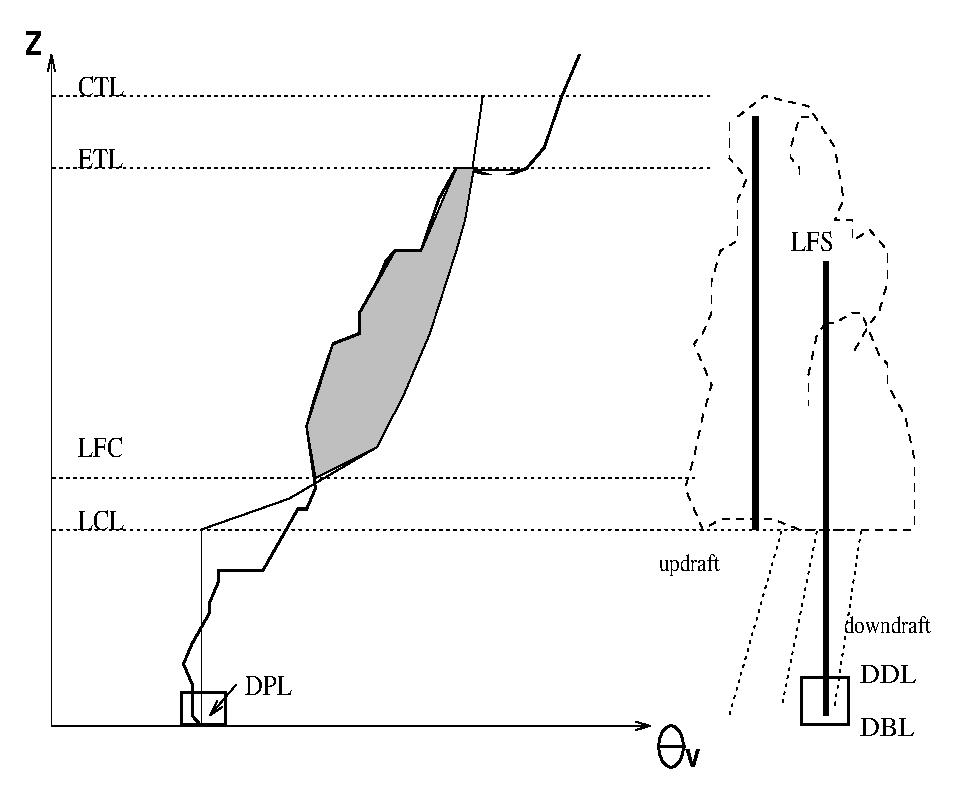
\includegraphics[width=10cm]{\EPSDIR/conv_fig1.eps}}
\caption{Environmental (thick solid line) and parcel sounding (thin solid line)
of $\theta_v$ in a deep convective cloud. The convective available
energy (CAPE) corresponds to the shaded area. The different key cloud
levels are related to condensation and buoyancy. The updraft and downdraft
regions are illustrated by the fat solid lines (the cloud is supposed
to precipitate).}
\label{conv_fig1}
\end{figure}

First, it is useful to define the
model cloud and a certain number
of important levels in the cloud that will be needed in the
following discussion. As illustrated in Fig.~\ref{conv_fig1}
the model cloud extends upward from the lifting condensation level (LCL) of
an air parcel with departure level DPL (DPL actually denotes a
60~hPa thick mixed layer) to
the cloud top level (CTL).
 The level of free convection (LFC)
is the level where the updraft becomes positively buoyant with respect
to the environment,
and the equilibrium temperature level (ETL) is
the level where the buoyancy of the updraft redrops to zero.
The convective available potential energy is defined as the positive area
(from the LFC to the ETL) between
the incloud virtual potential temperature sounding and the environmental
sounding.  The downdraft
originates within the cloud at the level of free sink (LFS), and extends down
to the downdraft base level (DBL). All downdraft mass is detrained over
a fixed layer extending from DDL to DBL.
Finally, note that the DPL and the DBL are
of course not necessarily equal to the surface level, the present figure serving
only as an example.


The following discussion of the different parts of the convection
scheme is straightforward in the way that it closely follows the sequential
structure of the scheme.



\subsection{Trigger function}

At present time, the physical processes initiating convection
are not well understood. There is no general criterion that tells
us when we should allow for convective overturning of the atmosphere; i.e.
when we should allow a moist convective parcel to overcome the stable
layer at cloud base and to have access to the CAPE that is stored aloft
due to large scale forcing associated with
e.g. midlatitude frontal systems, upper level jets or tropical waves.
However, another important
issue is the determination of the moist source layer for convection that
will be lifted up and will finally determine the properties of the
convective cloud (cloud top level, precipitation, etc.).
It turns out that over the tropical ocean this initial
moist layer corresponds to the 500-m deep boundary layer (Raymond 1995)
and the most difficult
problem is to locate the convection. However, in midlatitude convection,
especially at night time, convection might root at upper
atmospheric levels.

The numerical formalism is as follows.
Starting from the ground level, we first
construct an at least 60-hPa deep mixed layer with mean potential
temperature
$\overline{\theta}^{mix}$ and vapor mixing ratio $\overline{r}_v^{mix}$.
Then this mixed air parcel is lifted
without entrainment to its LCL.
We directly determine the temperature at the LCL using an
algorithm proposed by Davies-Jones (1983), and
compute the pressure at the LCL as
$P({\rm LCL})=P_{00}[T({\rm LCL})/\theta^{mix}]^{C_{pd}/R_d}$, where
$P_{00}$ is the reference pressure.
The air parcel is unstable with respect to moist
convection if at the LCL

\beq
\overline{\theta}_v^{mix}-\overline{\theta}_v+\Delta T/\Pi\,\,>0,
\label{dt}
\eeq
\noindent
with $\theta_v$ the virtual potential temperature, and
with the Exner function defined as $\Pi=(P/P_{00})^{R_d/C_{pd}}$. For shallow
convection the temperature increment $\Delta T$ is simply set to 0.2~K. For
deep convection $\Delta T$ is intended to crudely trigger/suppress
convection as a function of grid-scale motion, where it is defined by
$\Delta T = \pm c_{w}\,\,\,\vert \overline{w}\vert^{1/3}$,
with $c_w$=6 (K  m$^{-1/3}$ s$^{1/3}$).  The sign of $\Delta T$ is
equal to the sign of $\overline{w}$. As the large-scale vertical
velocity varies quasi-linearly as a function of the grid size, it
is normalized by $\overline{w}
\sqrt{A}/\Delta x_{ref}$,  with
$\Delta x_{ref}$ the 25-km reference grid space. Furthermore,
we test if the air parcel is able to produce a sufficient cloud depth
(at least 3~km for deep convection, and 500~m for shallow convection) by
lifting the  mixed layer parcel conserving the equivalent potential temperature
$\theta_e(\overline{\theta}^{mix},\overline{r}_v^{mix})$, and searching for the
intersection with the environmental saturated curve
$\theta_{es}(\overline{T})$ (see e.g. Raymond 1995).
If the air parcel is stable with
respect to moist convection or if its probable cloud thickness
is smaller than the specified value, the above procedure
is repeated starting at the next higher 60-hPa mixed layer, and so on.


\subsection{Updraft}

Updrafts are assumed to originate at the DPL, entrain environmental air
in the mixed layer, and then undergo undilute ascent up to the LCL.
Starting from the LCL the thermodynamic characteristics of the
updraft  are computed assuming conservation (except from
precipitation processes)
of enthalpy or "liquid water static energy" $h_{il}$ and total
water mixing ratio $r_w$

\begin{eqnarray}
h_{il}&=& C_{pm} T - L_v r_c - L_s r_i + ( 1 + r_w ) g z\label{conv-eqh}\\
r_w&=&r_v+r_c+r_i\label{conv-eqr}.
\end{eqnarray}
\noindent
where the specific heat of moist air is defined as
$C_{pm}= C_{pd} + r_w C_{pv}$, $g$ denotes the gravity constant, and
$r_v, r_c$ and $r_i$ denote the maxing ratios of water vapor and
non-precipitating cloud water/ice, respectively.
 A derivation of
$h_{il}$ is provided in the Appendix together with a definition of the
various thermodynamic constants and functions used.
The choice of $h_{il}$  is motivated by the fact
that it is linear, conserved in the presence of glaciation
processes, and easily allows to switch on/off glaciation processes in
the model.

The updraft computations are initiated at the LCL using
$h_{il}^u=C_{pm} T({\rm LCL}) + ( 1 + r_v^{mix} ) g z({\rm LCL})$ and $r_w^u=
r_v^{mix}$. The initial updraft mass flux is set to a unit value of
$M^u({\rm LCL})=\overline{\rho}\,w_{\rm LCL}\,\pi R_0^2,$
with a vertical velocity $w_{\rm LCL}$ of 1~m~s$^{-1}$ and
an updraft radius $R_0$ of 1500~m for deep and 50~m for shallow convection -
all the different parameter switches for deep and shallow convection are
summarized in Table \ref{conv-table1}.

\begin{table}
%\small
\caption{Parameters and  settings for deep and shallow convection}
\label{conv-table1}
\begin{center}
\begin{tabular}{||c|c|c||} \hline
{\bf Parameter} &{\bf deep}&\bf{shallow}\\
\hline \hline
cloud radius (m)&1500&50\\
minimum cloud thickness (m)&3000&500\\
adjustment time (h)&$0.5 < \tau<1$&3\\
$\Delta T$ (K) in "trigger"&computed from $\overline{w}$&0.2\\
downdraft&yes&no\\
precipitation&yes&no\\
\hline
\hline
\end{tabular}
\end{center}
\end{table}

Hereafter we switch to the discretized equations
on a vertical model grid $k$, with $k$ increasing with height.
The upstream operator is denoted by $\Delta\Psi=\Psi^{k+1}-\Psi^k$,
layer mean values are denoted by the additional superscript $m$.
If no superscript
is indicated we simply mean the current model level $k$. Furthermore, it
is convenient to denote the entrainment/detrainment rates $\epsilon$
and $\delta$ in mass flux units  kg s$^{-1}$ instead of units mass flux per
length as used in (\ref{eqc3})-(\ref{eqc10}).
In this notation the updraft mass flux as well as the updraft values of $h_{il}$
and $r_w$ change through mixing, detrainment and precipitation according to

\begin{eqnarray}
\Delta M^u&=&\epsilon^{um}-\delta^{um}\label{eqc0}\\
\Delta( M^u h_{il}^u)&=&\epsilon^{um}\overline{h}_{il}
-\delta^{um} h_{il}^{u} +M^{u(k+1)} (L_v \Delta r_r + L_s \Delta r_s)
\label{eqc1}\\
\Delta( M^u r_w^u)&=&\epsilon^{um}\overline{r}_w
-\delta^{um} r_w^{u}- M^{u(k+1)} (\Delta r_r + \Delta r_s).
\label{eqc2}
\end{eqnarray}

\noindent
The system (\ref{eqc0})-(\ref{eqc2}) is solved together with a
parameterization of microphysics and mixing that are described separately.

\subsubsection{Microphysics and updraft velocity}

The condensate mixing ratios  $r_c^u, r_i^u$ are deduced
from $h_{il}^u$ and $r_w^u$ using a saturation adjustment, and allowing
a gradual glaciation of the cloud in the temperature range between
268 and 248 K (see also Tao et al. 1989).
The liquid and solid precipitation
$\Delta r_r+\Delta r_s$ produced in each model layer is computed
 following Ogura and Cho (1973)
\beq
\Delta r_r+\Delta r_s=(r_c^{um}+r_i^{um}) (1- exp[-c_{pr} \Delta z/w^{um}]),
\label{eqPr}
\eeq
\noindent
where  $c_{pr}=0.02$ s$^{-1}$ is a condensate to precipitation
conversion factor. This formulation is essentially  based on the fact
that in high speed updrafts precipitation particles  do not have time to
form or are carried upward by the draft.
The updraft vertical velocity $w^u$ is evaluated with the aid of

\beq
\Delta( (w^u)^2) ={2 g\over 1+\gamma}
\left[{\theta_v^{um}-\overline{\theta}_v^m\over\overline{\theta}_v^m}\right]
\Delta z - 2{\epsilon^u\over M^u} (w^u)^2,
\label{eqc4}
\eeq
\noindent
where  $\theta_v=\theta (1+R_v/R_d\,\,r_v)/(1+r_w)$, and
$\gamma=0.5$ is the virtual mass coefficient that
approximately takes into account non-hydrostatic pressure perturbations
(Kuo and Raymond 1980).
The last term of the rhs of
(\ref{eqc4}) accounts for zero environmental momentum.
The vertical velocity is  also used to compute the cloud top level CTL,
which is defined as the level where $(w^u)^2$ becomes negative.
Finally, the total
precipitation flux produced by the updraft is simply given by
\beq
{\rm Pr}=\sum_{k={\rm LCL}}^{k={\rm CTL}}[\Delta r_r+\Delta r_s] M^u.
\eeq


\subsubsection {Entrainment and detrainment}

Unfortunately, the performance of a plume cloud model critically depends on
the specification of updraft entrainment/detrainment rates which are
functions of the cloud radius, and are generally
assumed to be constant with height. We initially adopted the
mixing formalism proposed by Kain and Fritsch (1990) where an
ensemble of mixed parcels is generated, with
positively buoyant parcels supposed to follow the cloudy updraft (entrain)
and negatively buoyant parcels supposed to detrain.
Denoting the fractional amount of environmental mass
that just yields a neutrally buoyant mixture  as $\chi_c$, the
net environmental entrainment rate and the updraft entrainment rate
are given by


\begin{eqnarray}
\epsilon^u&=&\Delta M_t\int_0^{\chi_c} \chi\,\,\, f(\chi) d\chi
\label{eqentr}\\
\delta^u&=&\Delta M_t\int^1_{\chi_c} (1-\chi) f(\chi) d\chi
\label{eqdetr}\\
\Delta M_t&=&M^u c_{\rm etr}\Delta z/R_0,
\label{eqMt}
\end{eqnarray}

\noindent
where $\Delta M_t$ with $c_{etr}=0.2$
is the total rate at which mass enters the transition
region between clear and cloudy air (Simpson 1983); $f(\chi)$ is a
Gaussian type distribution satisfying $f(0)=f(1)=0$ (Kain and Fritsch 1990).


The critical mixed fraction $\chi_c$
is solved for directly, knowing that the virtual temperature difference between
updraft-environment mixtures and that of the unmixed environment varies
linearly as a function of the environmental mass fraction $\chi$
(see Fig. \ref{conv_fig2}). The zero crossing of this curve is evaluated from

\begin{figure}
\centerline{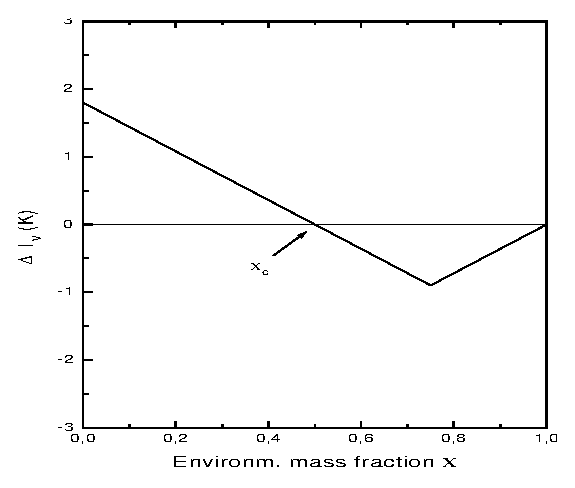
\includegraphics[width=10cm]{\EPSDIR/conv_fig2.eps}}
\caption{Plot of typical virtual temperature differences between
updraft-environment mixtures and that of the environment as a
function of the fraction of environmental mass in the mixtures.}
\label{conv_fig2}
\end{figure}

\beq
\theta_v^{mix}-\overline{\theta}_v=0=\theta_v^u-\overline{\theta}_v
- {\theta_v^u-\theta_v^{mix}\over\chi} \chi_c
\eeq
\noindent so that $\chi_c$ is given by

\beq
\chi_c={\theta_v^u-\overline{\theta}_v\over
         {\theta}_v^u-\theta_v^{mix} }   \chi; \quad \chi=0.1;
         \quad 0\le\chi_c\le 1;
\label{eqx5}
\eeq
\noindent
we use a small value of 0.1 for $\chi$ which is
supposed to be smaller than the critical value. $\theta_v^{mix}$ is
determined as a function of $h_{il}^{mix}$ and $r_w^{mix}$, where
$h_{il}^{mix}=\chi \overline{h}_{il}+(1-\chi)h_{il}^u$; idem for $r_w^{mix}$.

However, it turned out that in deep convective situations this mixing formulation often 
 produced $\epsilon^u>\delta^u$ so that the convective mass flux always increased with height,
and the upper-level mass flux was overestimated.
 Therefore, this mixing procedure was only retained for shallow convection. For deep convection
we simply use vertically constant entrainment/detrainment rates with 
 $\epsilon^u=\delta^u=0.5 \Delta M_t$.



\subsubsection{Updraft flow summary}

The updraft computations are an important
part of the convection scheme as here we build up a characteristic
precipitating cloud whose nominal mass flux is later modified
by the closure assumption. The
updraft computations can be summarized as follows:

1) Update CAPE for undilute ascent, i.e. assuming conservation of undilute
 $\theta_e$  at the LCL.

2) Estimate $r_c^u$ and $r_i^u$ at level $k+1$ setting
$h_{il}^u(k+1)=h_{il}^u(k), r_w^u(k+1)=r_w^u(k)$, and applying a
saturation adjustment procedure defined.

3) Compute $\theta_v^u(k+1)$ and square of vertical velocity using the
just computed values of $r_c^u$ and $r_i^u$ in (\ref{eqc4}).

4) Compute precipitation produced in model layer using (\ref{eqPr}).
Update total precipitation.

5) Update $r_c^u, r_i^u, h_{il}^u, r_w^u$ at level $k+1$
for precipitation.

6) Compute entrainment and detrainment rates at level $k+1$ using

7) Compute final values of updraft mass flux, $h_{il}^u, r_w^u$
at level $k+1$ using (\ref{eqc1})-(\ref{eqc2}).

8) Exit the updraft computations when the CTL is attained, i.e. when
the updraft velocity becomes negative.

9) Adjust the updraft mass flux to reflect a linear decrease of the mass
flux between the ETL and the CTL.


\subsection{Downdraft}

In contrast to the updraft computations
where condensate production and glaciation
processes are important and therefore $h_{il}$ is a very convenient
variable, the downdraft computations  become
simplified when using the equivalent potential temperature
$\theta_e$ as it implicitly takes into account the evaporational
cooling effect. The definition of $\theta_e$ is taken from Bolton (1980)
and proved to be highly accurate

\beq
\theta_e= T (P_{00}/P)^{R_d/C_{pd}(1-0.28 r_v)}
{\rm exp}[(3374.6525/T - 2.5403) r_v (1+0.81 r_v)].
\eeq

\noindent
The downdraft is assumed to be driven by cooling through melting and
evaporation of precipitation.
It originates at the level of free sink (LFS),
defined by the level of minimum environmental saturated $\theta_e$
between the LCL and the ETL.
The initial values of the downdraft mass flux, $\theta_e$ and moisture at
the LFS can be estimated as follows
\beq
M^d(LFS)= - (1-{\rm Pr_{eff}}) M^u(LCL)
\eeq

\noindent
where the precipitation efficiency Pr$_{\rm eff}$ is given as a function
of wind shear and cloud base height (Zhang and Fritsch 1986).
The initial humidity is obtained by mixing updraft and environmental air
\beq
r_w^d({\rm LFS})=\chi \overline{r}_w+(1-\chi)r_w^u; \quad
\chi=(\theta_e^u-\overline{\theta}_{es})/
(\theta_e^u-\overline{\theta}_e ).
\label{ee}
\eeq
\noindent
 This definition of the mixed fraction
 gives a very smooth variation of $\chi$, with a value
 that is close to $\chi_c$ defined in (\ref{eqx5}).
According to (\ref{ee})  the value of $\theta_e^d$ at the LFS is
set to its saturated environmental value corrected by melting effects,
with  the cooling due to melting estimated by
$\Delta T_{\rm melt}=
L_m/C_{ph}[r_w^u({\rm LCL})-r_w^u({\rm CTL})].
$
 This method is motivated by the fact
that the amount of downdraft mass flux is dependent on the total downdraft
evaporation rate which is not known initially and is itself dependent on
the magnitude of the melting effect. We know the amount of solid
precipitation but we do not know the amount of ice that is evaporated in
the downdraft.


The following equations are used to compute the downdraft properties
starting from the LFS down to the downdraft base level (DBL)
which is defined as the level where
$\theta_{e}^d(\rm{LFS}) >\overline{\theta}_{es}(\overline{T})$.


\begin{eqnarray}
\epsilon^d&=&-M^d({\rm LFS}) c_{\rm etr} \Delta z/R_0;\,\,\, k>{\rm DDL}\\
\delta^d&=&0; \quad\quad\quad\quad\quad\quad\quad\quad\quad\, k>{\rm DDL}\\
\Delta M^d&=&\epsilon^d\\
\Delta (M^d\theta_e^d)&=&\epsilon^d\overline{\theta}_e
\label{eqdt} \\
\Delta (M^d r_w^d)&=&\epsilon^d\overline{r}_w.
\label{eqdq}
\end{eqnarray}

\noindent
Note that $M^d$ is negative but $\epsilon^d$ and $\delta^d$ are positive.
All downdraft detrainment is assumed to occur over the 60~hPa
deep layer DDL-DBL (Fig. \ref{conv_fig1}).
For the closure adjustment procedure we will need the values of
$h_{il}^d$. As $\delta^d$ is zero everywhere apart from the
detrainment layer, we only
need to compute the values of $h_{il}^d$ for this layer. It is
computed from  $\theta_e^d$ and $r_w^d$.
The total downdraft evaporation rate is estimated using a specified
value of 90\% for the relative humidity. If the actual value
of humidity in the downdraft in the detrainment layer
is less than the specified
value, water is evaporated to give the required value. If no
water is evaporated, no downdraft is allowed and the
downdraft mass flux is set to zero.


\subsection{Closure}

Finally, a closure assumption is needed to control the intensity of
convection.  Here we adopt
a Fritsch Chappell type closure which is based on the assumption that all
convective available potential energy (CAPE) in a grid element is removed
within an adjustment period $\tau$. For deep convection $\tau$ is set
to the advective time period
$\tau=\sqrt{A}/\vert\vec v\vert$, with $\vec v$ the mean
horizontal wind vector between the LCL and the 500-hPa level, and is limited by
 0.5~h $< \tau <$ 1~h. The upper limit roughly corresponds to one life cycle
 of a convective cloud.
For shallow convection an adjustment time $\tau$ of 3~h is used.
With the aid of the above presented cloud model we have already
computed the initial guess updraft and downdraft mass fluxes
and the corresponding
entrainment/detrainment rates. Therefore, we are now able to compute
the final convectively-adjusted environmental values
(see also the main mass flux equations (\ref{eqc10}))
using a time integration over $\tau$ together with an iterative procedure

\begin{eqnarray}
\overline{\Psi}^{(n+1)}=\overline{\Psi}^{(n)}+(\tau/m_t)\,\,
\bigg[&-&\Delta( \tilde M^{(n)}\overline{\Psi}^{(n)})-
[\epsilon^{u(n)}+\epsilon^{d(n)}]\,\,
\overline{\Psi}^{(n)}\nonumber\\
&+&\delta^{u(n)}\Psi^{u}+\delta^{d(n)}\Psi^{d}\bigg]
\label{eqTa}
\end{eqnarray}


\beq
\tilde M=\overline{\rho}\tilde w A;\quad
\tilde w=\int(\partial\tilde w/\partial z) dz;\quad
\left({\partial\tilde{w}\over\partial z}\right)=
{\epsilon^u+\epsilon^d-\delta^u-\delta^d\over m_t},
\label{eqTb}
\eeq


\noindent
where $n$ denotes the iteration number,
$\Psi$ stands for either $h_{il}$ or the various water species  $r_w, r_c, r_i$.
The total mass of the model layer is denoted by $m_t$,
 and  $\tilde M$  is the compensating environmental mass flux.
The esssential point of the present adjustment procedure is that only
the environmental values  $\Psi= h_{il}, r_w, r_c, r_i$ are updated
and  the mass fluxes are adjusted
in the closure adjustment procedure, but no updraft or
downdraft computations are repeated so that the updraft and downdraft values
of the thermodynamic variables keep unchanged.

Now, computing the new environmental values of $\theta$ and $r_v$ from
$\overline{h}_{il}$ and $\overline{r}_w$
using (\ref{conv-eqh})-(\ref{conv-eqr}),
we can compute $\overline{\theta}_e$ and a new value of
CAPE  by using undilute parcel ascent

\begin{eqnarray}
{\rm CAPE^{(n+1)}}&=&
\int^{\rm ETL}_{\rm LCL^{(n+1)}} g
\left[ {
\overline\theta_e^{(n+1)}({\rm DPL})
\over\overline{\theta}_{es}^{(n+1)}  } -1 \right]\, dz,
\label{ecap}
\end{eqnarray}

\noindent
where the new value LCL$^{(n+1)}$ is obtained from
$\overline{\theta}_v^{(n+1)}$(DPL) by
the same procedure as used in the trigger function. The use of the
conserved variable $\overline{\theta}_{e}(DPL)$ instead of $\theta_v^u$
in (\ref{ecap}) is motivated by the fact that this formulation allows to
determine CAPE directly without executing additional updraft computations.

Then, at all model levels the updraft and downdraft mass fluxes as well as
the entrainment/detrainment fluxes and the precipitation flux
are multiplied by the adjustment factor
\beq
F_{adj}^{(n+1)}=F_{adj}^{(n)}{{\rm CAPE}^{(0)}
\over{\rm CAPE}^{(0)}-{\rm CAPE}^{(n+1)}},
\label{eqFa}
\eeq

\noindent
where ${\rm CAPE}^{(0)}$ is the initial value of CAPE.
The above described procedure
(\ref{eqTa})-(\ref{eqFa}) is repeated until
${\rm CAPE}^{(n+1)} < 0.1\,\, {\rm CAPE}^{(0)}$.
At the end of the adjustment procedure the final convective tendencies
are simply evaluated as
\beq
 {\partial\overline{\Psi}\over\partial t}\bigg\vert_{\rm conv}
 =(\overline{\Psi}^{(n)}-\overline{\Psi}^{(0)})/\tau,
\label{eqTH}
\eeq
where $\Psi$ now stands for either $\theta, r_v, r_c, r_i$.

A final remark concerns the conservation properties of the scheme, a
point that is particularly important for long time or global applications.
The scheme is designed to conserve mass and energy
as can be verified numerically from the  integral relationships

\begin{eqnarray}
\int_0^{\rm CTL}{(\epsilon^u+\epsilon^d-\delta^u-\delta^d)
\over m_t} dz = 0
\end{eqnarray}
\begin{eqnarray}
\int_{0}^{\rm CTL}  \left( {\overline{\rho}\over\rho_l}\right)
{\partial\overline{r}_w\over \partial t}\bigg\vert_{\rm conv} dz &=&
{{\rm Pr}\over \rho_l A }\\
\int_0^{\rm CTL} \left( {\overline{\rho}\over\rho_l}\right)
 {\partial\overline{h}_{il}\over\partial t}\bigg\vert_{\rm conv} dz &= &
L_v {{\rm Pr}\over \rho_l A }
\label{econs}
\end{eqnarray}

\noindent
where
 $\rho_l$ is the density of liquid water, and
${\rm Pr}\,\,\rho_l^{-1} A^{-1}$,
 is the adjusted surface precipitation flux in m s$^{-1}$.

\section{Discussion}
Our aim was to design a parameterization that incorporates the effects of the
essential physics of moist convection while remaining as straightforward and
numerically efficient as possible.  In adhering to these guidelines, however,
it is inevitable that numerous simplifications of real physical processes become
necessary.  

The limitations of a convective plume model to represent properties of a cloud ensemble
are discussed in Warner (1970), Raymond and Blyth (1986), and Lin and Arakawa (1997). 
To limit these drawbacks, we also developed an ensemble version of the code, where
the deep part can be called several times using different entrainment/detrainment rates
(=different cloud radius), and different temperature/moisture perturbations for triggering.
The resulting convective tendency is then the sum of the shallow part and the deep
convective part (which is an average of the convective tendencies and mass fluxes  of 
its individual ensemble members).



In the case of the present parameterization, an explicit dependence on
grid-length is included in two places.  First, grid-resolved vertical velocity,
as it is used in the trigger function (see discussion related to (5))
is scaled as a linear function of grid length.  Second, the convective time
period is computed as the advective time period, based on the mean wind speed in
the cloud layer and the model grid-length.  This time period is constrained to
be between 0.5 and 1 hour, however.
In addition to these implicit sensitivities to horizontal resolution, certain
physical processes have been neglected in the current parameterization.
For example, convective transport of momentum is not yet included, but could be
easily done using the scheme equations for passive tracers together with a pressure
perturbation term (Kershaw and Gregory 1997) 
Also, we do not explicitly account for mesoscale transports
that might give a substantial contribution to the mass flux at upper levels
(Donner 1993; Betts 1997; Alexander and Cotton 1998),
but the significance of this is largely unknown.
This parameterization contains several parameters that are difficult to assess.
 However, extensive testing
revealed minimal sensitivity to the values used for most of them, within a range
of reasonable values.  The most significant sensitivities appear in relation to
specification of cloud radius (determining entrainment/detrainment), the
precipitation efficiency (used to drive downdrafts), and to a lesser extent the
adjustment time scale.

Finally, lets also mention a limitation that is related to the effects of
convective downdrafts.   
In the atmosphere, convectively generated "cold pools" often spread out
over significant areas in the vicinity of thunderstorms, and the leading edge of
this cold outflow can be a region of active generation of new convective cells.
Since  prognostic variables are represented as horizontally-averaged values in
each layer within a grid-column, parameterization schemes introduce 
the effects of downdrafts as a mean cooling and drying of individual layers.
When these stabilizing tendencies are introduced as a mean effect, parameterized
convection may "turn off" due to  cooling and drying from parameterized downdrafts,
whereas in reality only a
portion of the total area represented by a grid element might experience intense
downdraft cooling. Thus 
parameterization schemes may have a tendency to
underpredict convective overturning at coarser resolutions.  A possible solution
for this problem would be to allow for partial coverage by downdraft outflow and
appropriate subgrid-scale forcing associated with outflow propagation (Liang et
al. 1998).

\section{Appendix}

\subsection{Definition of latent and specific heats}
The  specific latent heats of vaporisation, sublimation
and melting as a
function of temperature are defined by

\begin{eqnarray}
L_v(T)&=&L_v(T_t)+(C_{pv}-C_l) (T-T_t)\label{Lv}\\
L_s(T)&=&L_s(T_t)+(C_{pv}-C_s) (T-T_t)\label{Ls}\\
L_m(T)&=&L_s(T)-L_v(T)\label{Lm},
\end{eqnarray}


\noindent
with
\beq
T_t=273.16;\quad L_v(T_t)=2.5008\times 10^6
\quad L_s(T_t)=2.8345\times 10^6,
\eeq
\noindent
where $T_t$ is given in K and where the specific heats
for phase change
are given in J kg$^{-1}$. The specific heat constants
are defined as
\beq
C_{pv}=4\,\,R_v;\quad C_l=4.218\times 10^3;\quad C_s=2.106\times 10^3,
\eeq
\noindent
with $R_v$=461.525 J kg$^{-1}$ K$^{-1}$. The gas constant and specific
heat for dry air are defined as $R_d$=287.06 J kg$^{-1}$ K$^{-1}$ and
$C_{pd}= 7/2 R_d$.

\subsection{Derivation of $h_{il}$}

Following Dufour and van Mieghem (1975)  an accurate and
natural formulation of $h_{il}$ can be derived from the
enthalpy equation

\beq
C_{ph}  dT - T ( R_d + r_v R_v) d{\rm ln}P = d(L_v r_c + L_s r_i)
-\left[r_c{dL_v\over dT}+ r_i{dL_s\over dT}\right] dT,
\label{cph}
\eeq
\noindent
with $C_{ph}=C_{pd}+r_v C_{pv}+r_c C_l+r_i C_s$.
Making use of the hydrostatic approximation and the relations
(\ref{Lv})-(\ref{Lm}), (\ref{cph}) can be integrated to obtain
\beq
h_{il}= C_{pm} T - L_v r_c - L_s r_i + ( 1 + r_w ) g z,
\eeq
\noindent
with $C_{pm}= C_{pd} + r_w C_{pv}$.

\subsection{Definition of saturation mixing ratios}

The saturation pressure for water vapor over liquid water and
ice is derived from an integration of the Clausius-Clapeyron
equation

\begin{eqnarray}
e_{sl}(T)&=& exp\left[\alpha_l-{\beta_l\over T}-\gamma_l {\rm ln}(T)\right]\\
e_{si}(T)&=& exp\left[\alpha_s-{\beta_s\over T}-\gamma_s {\rm ln}(T)\right],
\end{eqnarray}

\noindent where
\beq
\alpha_l={\rm ln}[e_s(T_t)]+{\beta_l\over T_t}+\gamma_l {\rm ln}(T_t);
\quad
\beta_l={L_v(T_t)\over R_v}+\gamma_l T_t\nonumber
\label{eqab}
\eeq

\beq
\gamma_l={(C_l-C_{pv})\over R_v},
\label{eqy}
\eeq

and $e_s(T_t)=$611.14 Pa.
The corresponding coefficients for the saturation pressure over ice are
obtained by simply replacing in (\ref{eqab}) and (\ref{eqy})
the index $l$ (liquid) by the index $s$ (solid) and by replacing
$L_v$ by $L_s$.
Finally, the saturated water vapor mixing ratio is defined as
$r_{vs}(T)=(m_v/m_d) (e_s(T)/P-e_s(T)),$
with $m_v/m_d=R_d/R_v=0.622$ the ratio of dry air to water vapor Mol mass.

\subsection{Precipitation efficiency}
Defining the windshear by

\beq
S={\left\vert\vec v({\rm CTL})-\vec v ({\rm LCL})
\right\vert\over z({\rm CTL})-z({\rm LCL})}
{\vert\vec v({\rm CTL})\vert-\vert\vec v({\rm LCL})\vert\over
\big\vert\vert\vec v({\rm CTL})\vert-\vert\vec v({\rm LCL})\vert\big\vert},
\eeq

\noindent
with $\vec v$ the horizontal
wind vector, the precipitation efficiency as a function of wind shear
is expressed as

\beq
{\rm Pr_{Sef}}=1.591-0.639\, S +0.0953\, S^2-0.00496\, S^3.
\label{pref1}
\eeq

The precipitation efficiency as a function of cloud base height is
given as

\begin{eqnarray}
{\rm Pr_{Zef}}=0.967&-&0.7 z_b +1.62\times 10^{-1}z_b^2-1.26\times 10^{-2} z_b^3
\nonumber\\
&+&4.27\times 10^{-4} z_b^4-5.44\times 10^{-6} z_b^5,
\label{pref2}
\end{eqnarray}

\noindent
with $z_b$ the height difference between the LCL and the model surface level
normalized by a cloud base height of 3280~m. Both ${\rm Pr_{Sef}}$
and ${\rm Pr_{Zef}}$ are limited to values between 0.4 and 0.92.
Finally, the actual precipitation efficiency is given by
${\rm Pr_{eff}}=0.5({\rm Pr_{Sef}}+{\rm Pr_{Zef}})$.
\noindent



\section{References}
%\section*{References}

\noindent
\por
Alexander, G. D., and W.~R. Cotton, 1998:
The use of cloud resolving simulations of mesoscale convective
systems to build a mesoscale parameterization scheme.
{\it J. Atmos. Sci.}, {\bf 55}, 2137-2161.

\por
Arakawa, A., and W. H. Schubert, 1974: Interaction of a cumulus
cloud ensemble with the large-scale environment: Part I.
{\it J. Atmos. Sci.}, {\bf 31}, 674-701.

\por
Anthes, R. A., 1977: A cumulus parameterization scheme utilizing
a one-dimensional cloud model. {\it Mon. Wea. Rev.}, {\bf 105}, 270-286.

\por
Bechtold, P., E. Bazile, P. Mascart and E. Richard, 2001:
A Mass flux convection scheme for regional and global models.
{\it Quart. J. Roy. Meteor. Soc.}, {\bf 127}, 869-886.

\por
Bechtold, P., J. L. Redelsperger, I. Beau, M. Blackburn, S. Brinkop,
J. Y. Grandpeix, A. Grant, D. Gregory, F. Guichard, C. Hoff
and E. Ioannidou, 2000: A GCSS model
intercomparison for a tropical squall line observed during TOGA-COARE.
II: Intercomparison of single-column models and a cloud-resolving model.
{\it Quart. J. Roy. Meteor. Soc.}, {\bf 126}, 865-888.

\por
Betts, A. K., and M. J. Miller, 1986: A new convective adjustment scheme.
Part II: Single column tests using GATE wave, BOMEX, ATEX, and arctic air-mass
data sets. {\it Quart. J. Roy. Meteor. Soc.}, {\bf 112}, 693-709.

\por
----------, 1997:
`The parameterization of deep convection'.
In {\it "The physics and parameterization of moist atmospheric convection"}
(Ed. R. K. Smith), {\it NATO ASI Series}, {\bf 505}, 255-279.

\por
Bolton, D., 1980: The computation of equivalent potential temperature.
{\it Mon. Wea. Rev.}, {\bf 108}, 1046-1053.

\por
Bougeault, P., 1985: A simple parameterization of the large-scale
effects of cumulus convection. {\it Mon. Wea. Rev.}, {\bf 113}, 2108-2121.

\por
Bretherton, C. S., and P. K. Smolarkiewicz, 1989: Gravity waves,
compensating subsidence and detrainment around cumulus clouds.
{\it J. Atmos. Sci.}, {\bf 46}, 740-759.

%\por
%Carpenter, R. L. Jr., K. K. Droegemeier, and A. M. Blyth, 1998:
%Entrainment and detrainment in numerically simulated cumulus congestus
%clouds. Part I: General results.
%{\it J. Atmos. Sci.,} {\bf 55,} 3433-3439.

\por
Charney, J., and A. Eliassen, 1964: On the growth of the hurricane
depression. {\it J. Atmos. Sci.,} {\bf 21,} 68-75.

%\por
%Courtier, P., and J.-F. Geleyn, 1988:
%A global numerical weather prediction model with variable
%resolution: Application to the shallow-water equations.
%{\it Quart. J. Roy. Meteor. Soc.,} {\bf 114,} 1321-1346.

\por
Davies-Jones, R. P., 1983: An accurate theoretical approximation for
adiabatic condensation temperature. {\it Mon. Wea. Rev.},
{\bf 111}, 1119-1121.

\por
Donner, L. J., 1993: A cumulus parameterization including mass fluxes,
vertical momentum dynamics, and mesoscale effects.
{\it J. Atmos. Sci.}, {\bf 50}, 889-906.

\por
-----------, C. J. Seman, and R. S. Hemler, 1999: Three dimensional cloud-system
modeling of GATE convection. {\it J. Atmos. Sci.}, {\bf 56}, 1885-1912.

\por
Dufour L., and J. van Mieghem, 1975: Thermodynamique de
l'atmosph\`ere. Institut Royal M\'et\'eorologique de Belgique, 278 pp.

\por
Emanuel, K. A., 1991: A scheme for representing cumulus convection in
large-scale models. {\it J. Atmos. Sci.}, {\bf 48}, 2313-2335.

\por
----------, 1997:
The problem of convective moistening.
In {\it "The physics and parameterization of moist atmospheric convection"}
(Ed. R. K. Smith), {\it NATO ASI Series}, {\bf 505}, 447-462.
%
%\por
%Feltz, W. F., William L. Smith, Robert O. Knuteson, Henry E. Revercomb,
%Harold M. Woolf, and H. Ben Howell, 1998: Meteorological applications of
%temperature and water vapor retrievals from the ground-based Atmospheric
%Emitted Radiance Interferometer (AERI).
%{\it J.  Appl. Meteor.,} {\bf 37,} 857-875.

\por
Fritsch, J. M., and C. F. Chappell, 1980: Numerical prediction of
convectively driven mesoscale pressure systems. Part I:
Convective parameterization. {\it J. Atmos. Sci.}, {\bf 37}, 1722-1733.

\por
Fritsch, J. M., R. A. Houze, R. Adler, H. Bluestein, L. Bosart,
J. Brown, F. Carr, C. Davies, R. H. Johnson, N. Junker, Y.-H. Kuo,
S. Rutledge, J. Smith, Z. Toth, J. W. Wilson, E. Zipser, and D. Zrnic, 1998:
Quantitative precipitation forecasting: Report of the eighth prospectus
development team, U. S. weather research program.
{\it Bull. Am. Meteorol. Soc.}, {\bf 79}, 285-299.


%\por
%Grabowski, W. W., and P. K. Smolarkiewicz, 1999: CRCP: A cloud resolving
%convection parameterization for modelling the tropical convecting
%atmosphere. {\it Physica D}, to appear.

\por
Gregory, D., and M. J. Miller, 1989: A numerical study of the parameterization
of deep tropical convection. {\it Quart. J. Roy. Meteor. Soc.},
{\bf 115}, 1209-1241.

\por
Gregory, D., and P. R. Rowntree, 1990:
A mass-flux convection scheme with
representation of cloud ensemble characteristics and stability
dependent closure. {\it Mon. Wea. Rev.}, {\bf 118}, 1483-1506.

\por
Grell, G. A., 1993: Prognostic evaluation of assumptions used by
cumulus parameterizations. {\it Mon. Wea. Rev.}, {\bf 121}, 764-787.

\por
Hu, Q., 1997: A cumulus parameterization based on a cloud model of
intermittently rising thermals. {\it J. Atmos. Sci.}, {\bf 54}, 2292-2307.

\por
Kain, J. S., and J. M. Fritsch, 1990: A one-dimensional
entraining/detraining plume model and its application in
convective parameterizations. {\it J. Atmos. Sci.},
{\bf 47}, 2784-2802.

\por
-----------, and -----------, 1993: Convective parameterization for mesoscale
models: The Kain-Fritsch scheme.
{\it Meteor. Monographs}, {\bf 46}, 165-170.

\por
Kershaw, R., and D. Gregory, 1997: Parameterization of momentum
transport by convection. Part I: Theory and cloud modelling results.
{\it Quart. J. Roy. Meteor. Soc.}, {\bf 123}, 1133-1151.

%\por
%Krueger, S. K.,  D. Gregory, M. W. Moncrieff, J.-L. Redelsperger
%and W.-K. Tao, 1996:
%GCSS Working Group 4: First Cloud-Resolving Model intercomparison
%Project. Case~2.
%{\it Technical Report}, available from University of Utah, Meteorological Department.

\por
Kuo, H. L., 1965: On formation and intensification of tropical cyclones
through latent heat release by cumulus convection.
{\it J. Atmos. Sci.}, {\bf 22}, 40-63.

\por
----------, and W. H. Raymond, 1980: A quasi-one-dimensional
cumulus cloud model and parameterization of cumulus heating
and mixing effects. {\it Mon. Wea. Rev.}, {\bf 108}, 991-1009.

\por
Kuo, Y.-H., J. F. Bresch, M.-D. Cheng, J. Kain, D. B. Parsons,
W.-K. Tao and D.-L. Zhang, 1997: Summary of a mini workshop on cumulus
parameterization for mesoscale models.
{\it Bull. Am. Meteorol. Soc.}, {\bf 78}, 475-490.

%\por
%Lafore, J. P., J. Stein, N. Asencio, P. Bougeault,
%V. Ducrocq, J. Duron, C. Fischer, P. Hereil, P. Mascart,
%J. P. Pinty, J. L.  Redelsperger, E. Richard
%and J. Vila-Guerau de Arellano, 1998:
%The Meso-NH Atmospheric Simulation System.
%Part I: Adiabatic formulation and control simulations.
% {\it Annales Geophysicae}, {\bf 16}, 90-109.

%\por
%LeMone, M. A., and M. W. Moncrieff, 1993: Momentum transort by convective
%bands: Comparisons of highly idealized dynamical models to observations.
%{\it Meteor. Monographs}, {\bf 46,} 75-92.

\por
Lin, C., and A. Arakawa, 1997: The macroscopic entrainment process of simulated
cumulus ensemble. Part II: Testing the entraining-plume model
{\it J. Atmos. Sci.}, {\bf 54}, 1027-1043.

\por
Liang, Q., G. S. Young, and W. M. Frank, 1998:  A convective wake parameterization
scheme for use in general circulation models. {\it Mon. Wea. Rev.}, {\bf 126},
456-469.

\por
Mallet, I., J.-P. Cammas, P. Mascart and P. Bechtold, 1999:
Effects of cloud diabatic heating on a FASTEX cyclone (IOP17) early
development. {\it Quart. J. Roy. Meteor. Soc.}, {\bf 125}, 3415-3438.

\por Manabe, S., and R. Strickler, 1964: Thermal equilibrium
of the atmopshere with a convective adjustment.
{\it J. Atmos. Sci.}, {\bf 21}, 361-385.

\por
Mapes, B. E., 1997:
 Equilibrium versus activation control of large-scale
variations of tropical deep convection.
In {\it "The physics and parameterization of moist atmospheric convection"}
(Ed. R. K. Smith), {\it NATO ASI Series}, {\bf 505}, 321-358.

\por
Moncrieff,~M.~W., D. Gregory, S. K. Krueger, J. L. Redelsperger, and
 W. K. Tao, 1997:
 GEWEX Cloud System Study (GCSS) working group 4:
 Precipitating convective cloud systems. {\it Bull. Am. Meteorol. Soc.},
 {\bf 78}, 831-845.

\por
Ogura, Y., and H.-R. Cho, 1973: Diagnostic determination of cumulus
populations from large-scale variables. {\it J. Atmos. Sci.},
{\bf 30}, 1276-1286.

\por
Ooyama, K., 1971: A theory on parameterization of cumulus convection.
{\it J. Meteor. Soc. Japan}, {\bf 49}, 744-756.

\por
Raymond, D. J., 1995: Regulation of moist convection over the
West Pacific warm pool. {\it J. Atmos. Sci.}, {\bf 52}, 3945-3959.

\por
----------, and A. M. Blyth, 1986: A stochastic mixing model for
nonprecipitating clouds.
{\it J. Atmos. Sci.}, {\bf 43}, 2708-2718.

%\por
%Redelsperger, J. L., P. R. A; Brown, F. Guichard, C. Hoff, M. Kawasima,
%S. Lang, T. Montmerle, K. Nakamura, K. Saito, C. Seman, W. K. Tao,
%and L. J. Donner, 2000:
% A GCSS model intercomparison for a tropical squall
% line observed during TOGA-COARE. Part I: Cloud-resolving models.
%{\it Quart. J. Roy. Meteor. Soc.}, to appear.

\por
Sun, W.-H., and P. A. Haines, 1996: Semi-prognostic tests of a new cumulus
parameterization scheme for mesoscale modeling.
{\it Tellus}, {\bf 48A}, 272-289.

%\por
%S\'en\'esi, S., Bougeault, P., Ch\`eze, J.-L., Cosentino, P. and
%Thepenier, R.-M.,
%1996:
%The Vaison-la-Romaine flash flood: Mesoscale analysis and predictability
%issues. {\it Weather Forecasting,} {\bf 11,} 417-442.

%\por
%Siebesma, A. P., and J. W. M. Cuijpers, 1995: Evaluation of parametric
%assumptions for shallow cumulus convection. {\it J. Atmos. Sci.,}
%{\bf 52,} 650-666.

%\por
%----------, 1998: Shallow cumulus convection. In {\it "Buoyant convection
%in geophysical flows"} (Eds. Plate et al.), {\it Kluwer Academic Publishers,}
%441-486.

\por
Simpson, J., 1983: Cumulus clouds: interactions between laboratory
experiments and observations as foundations for models.
{\it Mesoscale Meteorology}, D. K. Lilly and T. Gal-Chen, Eds., Reidel,
399-412.

\por
Slingo, J.~M., M. Blackburn, A. K. Betts, R. Brugge, K. D. Hodges,
B. J. Hoskins, M. J. Miller, L. Steenman-Clark, and J. Thuburn, 1994:
Mean climate and
transience in the tropics of the UGAMP GCM: Sensitivity to convective
parameterization. {\it Q. J. R. Meteorol. Soc.}, {\bf 120}, 881-922.

%\por
%Stein, J., E. Richard, J. P. Lafore, J. P. Pinty, N. Ascensio and
%S. Cosma, 1999: Meso-NH simulations with grid-nesting and ice-phase
%parameterization. {\it Meteor. Atmos. Phys.}, to appear

\por
Tao, W.-K., J. Simpson, and M. McCumber, 1989: An ice-water
saturation adjustment. {\it Mon. Wea. Rev.}, {\bf 117}, 231-235.

\por
Tiedtke, M., 1989: A comprehensive mass flux scheme for cumulus
parameterization in large-scale models.
{\it Mon. Wea. Rev.}, {\bf 117}, 1779-1800.

\por
Wang, J., and D. A. Randall, 1996: A cumulus parameterization based on
the generalized convective available potential energy.
{\it J. Atmos. Sci.}, {\bf 53}, 716-727.

\por
Warner, J., 1970: On steady-state one-dimensional models of
cumulus convection. {\it J. Atmos. Sci.}, {\bf 27}, 1035-1040.

%\por
%Warner, T. T., and H.-M. Hsu, 1999: Nested model simulation of moist convection:
%The impact of coarse-grid parameterized convection on fine-grid resolved
%convection through lateral boundary effects.  {\it Mon. Wea. Rev.} to appear

\por
Xie, S.-C., K.-M. Xu, R. T. Cederwall, P. Bechtold, A. D. Del Genio, S. A. Klein,
D. G. Cripe, S. J. Ghan, D. Gregory, S. F. Iacobellis, S. K. Krueger, U. Lohmann,
J. C . Petch, D. A. Randall, L. D. Rotstayn, R. C. J. Somerville, Y. C. Sud, 
K. von Salzen, G. K. Walker, A. Wolf, J. J. Yio, G. J. Zhang and M. Zhang, 2002:
Intercomparison and evaluation of cumulus parameterizations under summertime midlatitude
continental conditions. {\it Q. J. R. Meteorol. Soc.}, {\bf 128}, 1095-1135.

\por
Yanai, M., S. K. Esbensen, and J.-H. Chu, 1973: Determination of
bulk properties of tropical cloud clusters from large-scale heat and moisture
budgets. {\it J. Atmos. Sci.}, {\bf 30}, 611-627.

\por
Zhang, D.-L., and J. M. Fritsch, 1986: Numerical simulation of the
meso-$\beta$ scale structure and evolution of the 1977 Johnstown flood.
Part I: Model description and verification. {\it J. Atmos. Sci.},
{\bf 43}, 1913-1943.

%
%%%%%%%%%%%%%%%%%%%%%%%%%%%%%%%%%%%%%%%%%%%%%%%%%%%%%%%%%%%%%%%%%%%%%%%%%
%%%%%
% END OF CONTRIBUTION TO THE MESONH BOOK1: "Convection Scheme"
%%%%%%%%%%%%%%%%%%%%%%%%%%%%%%%%%%%%%%%%%%%%%%%%%%%%%%%%%%%%%%%%%%%%%%%%%
%%%%%




%\end{document}

%%%%%%%%%%%%%%%%%%%%%%%%%%%%%%%%%%%%%%%%%%%%%%%%%%%%%%%%%%%%%%%%%%%%%%%%%%%%%%
% CONTRIBUTION TO THE MESONH BOOK1: "Microphysical Scheme for Warm Clouds"
% Author : Evelyne Richard
% Original : October 15, 1997
% Update   : October 15, 1997
%%%%%%%%%%%%%%%%%%%%%%%%%%%%%%%%%%%%%%%%%%%%%%%%%%%%%%%%%%%%%%%%%%%%%%%%%%%%%%%

\chapter{Microphysical Schemes for Warm Clouds}
\minitoc
Three microphysical schemes for warm clouds are implemented into Meso-NH.
The most simple scheme is the Kessler one, a one-moment scheme that prognoses mixing ratio of cloud and rain water.
The two others are some two-moment schemes that predicts the mixing ratio and the concentrations of cloud and rain drops.
The C2R2 scheme is the most general one while the KHKO scheme is designed for stratocumulus.

\section{Kessler scheme}

%{\em by E. Richard}

\subsection{Equations}
We note $r_v$, $r_c$, and $r_r$ the water vapor, cloud water and rainwater
mixing ratios, as defined in MESO-NH. For any constituent,
$r$ is the mass of the
constituent divided by the reference mass of dry air.\footnote{Notice that
$\rho_{d\, ref}r = \rho_d \tilde r$ where  $\tilde r$ is the usual mixing ratio
i.e. the mass of the constituent divided by the mass of dry air.}
The consevation equations for these quantities are written:
\begin{eqnarray}
 &\dfrac{d}{dt}(  \rho_{d\,ref} r_v)&= \rho_{d\,ref} (P_{RE}-  P_{CON})\\
 &\dfrac{d}{dt}(  \rho_{d\,ref} r_c)&= \rho_{d\,ref}(- P_{RA} -  P_{RC}+  P_{CON})\\
 &\dfrac{d}{dt}(  \rho_{d\,ref} r_r)&= \rho_{d\,ref} (P_{RA} +  P_{RC} -  P_{RE}
+  P_{RS})
\end{eqnarray}
where $P$ designates the sources and where the subscripts
 $CON$, $RE$, $RA$, $RC$ and $RS$  respectively refer to the following processes:
evaporation/condensation, rain evaporation, accretion of cloud droplets by
raindrops, conversion of cloud droplets into raindrops (autoconversion),
and rain sedimentation.
Condensation/evaporation is a very fast process, it cannot be computed
explicitly and is obtained through an implicit saturation adjustment
procedure, taking subgrid-scale processes into account (see Chapter on the sub-grid condensation schemes).
All others terms are computed explicitly.


\subsection{Raindrops characteristics}
\subsubsection{Distribution}
Raindrops are assumed to follow a Marshall-Palmer distribution. The number of
raindrops whose diameter lies in the interval
$D$ and $D+dD$ is given by:
\begin{equation}
N(D)dD=N_0 \exp (-\lambda D) dD
\end{equation}
Observations for different types of rain show a range of values for
$N_0$ from
$0.4\ 10^7$ to $3.5\ 10^7$~m$^{-4}$. $N_0= 10^7$~m$^{-4}$
is a value frequently used.


The $\lambda$ parameter is obtained from
\begin{equation}
 \rho_{d\,ref} r_r=\int_0^\infty {\pi \over 6} \rho_{lw} D^3 N_0 \exp(-\lambda D)dD=
{\pi \rho_{lw} N_0 \over \lambda^4},
\end{equation}
which leads to
\begin{equation}
\lambda= \Big({\pi \rho_{lw} N_0 \over \rho_{d\,ref} r_r}\Big)^{1 \over 4}.
\end{equation}
\subsubsection{Fall velocity}
The terminal fall velocity for a raindrop of diameter $D$ is expressed as
\begin{equation}
V(D)=  \big( \dfrac{ \rho_{00}}{ \rho_{d\,ref}} \big)^{\alpha} aD ^{b},
\label{eqvterm}
\end{equation}
with $\alpha=0.4$, $a=842$~m$^{0.2}$/s and $b=0.8$, $\rho_{00}$ being the air
density at the reference pressure level $P_{00}$.
This parameterization follows Liu and Orville (1969) and includes the
effect of mean density variation as suggested by Foote and Du Toit (1969).

The rain terminal fall velocity is then given by
\begin{equation}
V_T \rho_{d\,ref} r_r= \int_0^\infty {\pi \over 6} \rho_{lw} D^3 V(D) N(D)dD,
\end{equation}
which leads to
\begin{equation}
V_T = {a \over 6} \big( {\rho_{00}\over \rho_{d\,ref}}\big) ^\alpha
{\Gamma(b+4)\over \lambda ^b},
\end{equation}
or
\begin{equation}
V_T= {a \over 6} \Gamma(b+4)\big( {\rho_{00}\over \rho_{d\,ref}}\big) ^\alpha
\big( {\rho_{d\,ref} r_r \over \pi \rho_{lw} N_0}\big)
^{b \over 4}.
\label{eqvterm2}
\end{equation}
\subsection{Explicit sources}

\subsubsection{Autoconversion}
The sole rainwater initiation mechanism is the autoconversion process which is
parameterized according to Kessler (1969).
The Kessler rate relies on intuitive considerations:
the autoconversion rate increases linearly with the cloud water content
$(\rho_{d\,ref} r_c)$ but
cloud conversion does not occur below a threshold value $ q_{crit}$.
\begin{equation}
P_{RC}= k\  \max( r_c - \dfrac{q_{crit}}{\rho_{d\,ref}}, 0)
\end{equation}
The parameters $k$ and $q_{crit}$ are
usually set to $10^{-3}$~s$^{-1}$ et $0.5$~g/m$^3$.

In the code $P_{RC}$ is written as:
\begin{equation}
P_{RC}= C1_{RC} Max ( r_c - \dfrac{C2_{RC}}{\rho_{d\,ref}}, 0)
\end{equation}
with $C1_{RC}= k$ and $C2_{RC}=q_{crit}$.


\subsubsection{Accretion}
Once embryonic precipitation particles are formed, rainwater mixing ratio
growth occurs
primarily by accretion of cloud water in the form
\begin{equation}
P_{RA}=\int_0^\infty {\pi \over 4}D^2 V(D) E  r_c N(D)dD,
\end{equation}
where E is the collision efficiency (here taken equal to 1).
After integration,
\begin{equation}
P_{RA}={\pi \over 4}a N_0( \dfrac{ \rho_{00}}{ \rho_{d\,ref}})^{\alpha}
 r_c{\Gamma(b+3) \over \lambda ^{b+3}}.
\end{equation}
After replacing $\lambda$,
\begin{equation}
P_{RA}={\pi \over 4}a N_0( \dfrac{ \rho_{00}}{ \rho_{d\,ref}})^{\alpha}
 r_c  \Gamma(b+3) \big( {\rho_{d\,ref} r_r \over \pi \rho_{lw} N_0}\big)
^{b+3 \over 4}.
\end{equation}
In the code $P_{RA}$ is written as:
\begin{equation}
P_{RA}= C_{RA}( \rho_{d\,ref})^{C'_{RA}-\alpha}  r_c ( r_r )^{C'_{RA}}
\end{equation}
with
$$ C_{RA}={\pi \over 4}a N_0( \rho_{00})^{\alpha} \Gamma(b+3)
\big( {1 \over \pi \rho_{lw} N_0}\big)
^{b+3 \over 4}$$
and $$C'_{RA}={b+3 \over 4}$$

The accretion and autoconversion sources are limited by the amount of available
cloud water. In the case where both processes are simultaneously operating,
accretion is computed first.

\subsubsection{Rain evaporation}
According to Pruppacher and Klett (1978, p~420), the evaporation rate of a drop
of diameter D is given by
\begin{equation}
D {dD \over dt} = {4S \bar f \over \rho_{lw} A}, \label{eq17}
\end{equation}
where $\bar f$ is a ventilation factor and
\begin{eqnarray}
S&=& {r_{vs}-r_v \over r_{vs}}, \\
A&=& {R_v T \over e_s(T) D_v} + {L_v(T) \over k_a T}({L_v(T) \over R_v T} -1)\\
 &\simeq &{R_v T \over e_s(T) D_v} + {L_v(T)^2 \over k_a R_v T^2}  .
\end{eqnarray}

$r_{vs}$ is the saturated vapor mixing ratio, $D_v$ is the diffusivity of water
vapor in air and $k_a$ is the heat conductivity of air.
For simplicity, $D_v$ and  $k_a$ are taken constants:
$D_v=2.26\ 10^{-5}$~m$^2$/s and $k_a= 24.3 \ 10 ^{-3}$~J/(msK).

$e_s$ is the saturation vapor pressure and is computed according to
\begin{equation}
\label{eq21}
e_s(T)= \exp \big( \alpha_w - {\beta_w \over T} - \gamma_w \ln (T) \big),
\end{equation}
with
\begin{eqnarray}
&\alpha_w   &= \ln (e_s(T_t))+{\beta_w \over T_t} - \gamma_w \ln (T_t), \\
&\beta_w   &= {L_v(T_t) \over R_v}\gamma_w T_t, \\
&\gamma_w  &= {C_l -C_{pv} \over R_v}.
\end{eqnarray}

$L_v$ is the latent heat of vaporization and is computed according to
\begin{equation}
L_v(T) = L_v(T_t) + (C_{pv} - C_l)(T-T_t).
\end{equation}
The ventilation factor $\bar f$ is given by
\begin{equation}
\bar f = 1 + F (Re) ^{0.5},\label{eq26}
\end{equation}
where $Re$ is the Reynolds number which can be expressed as
\begin{equation}
Re= {V(D) D \over \nu}, \label{eq27}
\end{equation}
$\nu$  being  the air kinematic viscosity which is here assumed to be constant:
$\nu=0.15 \ 10^{-4}$~kg/(ms).

$F$ is a ventilation coefficient taken equal to 0.22.

After replacing (\ref{eqvterm}) and (\ref{eq27}) in (\ref{eq26}), one gets
\begin{equation}
\bar f =  1 + F \big[ \big( {\rho_{00} \over \rho_{d\,ref}} \big) ^\alpha
{aD^{b+1}  \over \nu} \big] ^{0.5}.
\end{equation}
The integration of (\ref{eq17}) over the rain drop spectrum
leads to  the expression of the evaporation source
\begin{equation}
P_{RE} = {1 \over \rho_{d\,ref}}\int_0^{+\infty} {2 \pi S \bar f \over A} D N(D) dD.
\end{equation}
After replacing $\bar f$,
\begin{equation}
P_{RE} = {2 \pi S N_o \over A}{1 \over \rho_{d\,ref}} \big[ {1 \over \lambda ^2}
+ F ( {\rho_{00} \over \rho_{d\,ref}} )^{\alpha /2} ({a  \over \nu})^{1/2}
{\Gamma ({b+5 \over 2}) \over \lambda ^{{b+5 \over 2}}} \big],
\end{equation}
or
\begin{equation}
P_{RE} = {2 \pi S N_o \over A} {1 \over \rho_{d\,ref}} \big[
\big( {\rho_{d\,ref} r_r \over \pi \rho_{lw} N_o}\big) ^{1 \over 2}
+ F ( {\rho_{00} \over \rho_{d\,ref}} )^{\alpha /2} ({a  \over \nu})^{1/2}
\Gamma ({b+5 \over 2})
\big( {\rho_{d\,ref} r_r \over \pi \rho_{lw} N_o}\big) ^{b+5 \over 8} \big].
\end{equation}
In the code $P_{RE}$ is written as
\begin{equation}
P_{RE}= { S \over A}\big [ C1_{RE} (\rho_{d\,ref}) ^{-{1 \over 2}} (r_r) ^{1 \over 2} +
 C2_{RE} (\rho_{d\,ref} ) ^{C'_{RE}-1- \alpha/2} (r_r ) ^{C'_{RE}} \big],
\end{equation}
with
$$C1_{RE}=2 \pi  N_o ( {1 \over \pi \rho_{lw} N_o}) ^{1 \over 2}$$
$$C2_{RE}=2 \pi  N_o  F \big( \rho_{00} )^{\alpha /2} ({a \over \nu})^{1/2}
\Gamma ({b+5 \over 2})
\big( { 1 \over \pi \rho_{lw} N_o}\big) ^{b+5 \over 8} \big)$$
$$C'_{RE}={b+5 \over 8}$$

The rain evaporation source is limited by the amount of available rainwater.

\subsubsection{Rain sedimentation}
The sedimentation rate is given by
\begin{eqnarray}
&P_{RS} &= {1 \over \rho_{d\,ref}}{\partial \over \partial z} \int_0^\infty N(D)V(D) {\pi \over 6}
\rho_{lw} D^3 V(D)N(D) dD \\
&&= {1 \over \rho_{d\,ref}}{\partial \over \partial z} (V_T \rho_{d\,ref} r_r).
\end{eqnarray}

In the code, $P_{RS}$ is written as
\begin{equation}
P_{RS} = {1 \over \rho_{d\,ref}}{\partial \over \partial z} \big[ C_{RS}
(\rho_{d\,ref})^{C'_{RS}-\alpha} (r_r )^{C'_{RS}}\big],
\end{equation}
with
$$C_{RS}= {a \over 6} \Gamma(b+4)( \rho_{00}) ^\alpha
\big( {1\over \pi \rho_{lw} N_0} \big)^{b \over 4},$$
$$C'_{RS}={4+b \over 4}.$$

In order to maintain stability, the rain sedimentation source is computed with
a time splitting technique and with  an upstream differencing scheme. The small
time step used for this computation is determined from the CFL stability
criterion based on a maximum raindrop fall velocity $V_{TRmax}$ of 7~m s$^{-1}$.

The sedimentation rate can be alternatively calculated using a Probability Density Function (PDF)
-based approach. A general
description of the method is done in Geleyn et al. (2008). The sedimentation rate is given by

\begin{eqnarray}
&P_{RS} &= {1 \over \rho_{d\,ref}} {\partial \over \partial z} F_r
\end{eqnarray}

where $F_r$ is the sedimentation flux. The sedimentation flux is computed from the top to the 
bottom of the atmosphere following

\begin{eqnarray}
&F_r(j) &= P_1 {\Delta z \over \Delta t} \rho_{d\,ref} r_r + P_2 F_r(j-1)
\end{eqnarray}

$\Delta t$ is the time step and $\Delta z$ the thickness of the layer. 
$P_1$ and $P_2$ are computed as in Geleyn et al. (2008) in the case where the PDF
of the fall speeds of the drops is a simple step function


\begin{eqnarray}
&P_1 &= \min\left(1,{V_{T1} \Delta t \over \Delta z} \right)  \\
&P_2 &= \max\left(0, 1 - {\Delta z \over V_{T2} \Delta t} \right)
\end{eqnarray}

$V_{T1}$ and $V_{T2}$ are the terminal velocities of the two groups of drops. The first one is computed
using equation (\ref{eqvterm2}) and $r_r$ of the level $j$. $V_{T2}$ is computed with the same equation but
using a mixing ratio representative of the incoming flux

\begin{eqnarray}
&r'_r &= {\Delta t \over \rho_{d\,ref} \Delta z} F_r(j-1) 
\end{eqnarray}

This method is unconditionally stable and avoids the use of a time splitting technique.


\subsection{Implicit sources}
Once the explicit sources are computed, the condensation/evaporation rate is
obtained through a saturation adjustment procedure following Langlois (1973).
If $T^*$ and $r_v^*$ are the temperature and vapor mixing ratio obtained after
adding the explicit sources, we seek the zero-crossing of $F(T)$, defined as
\begin{equation}
F(T)= (T-T^*) + {L_v(T) \over C_{ph}} (r_{vs}(T)-r_v^*).
\end{equation}
To obtain a rapidly convergent algorithm, Langlois suggests to use a
generalized
Newton-Raphson procedure which employs the first and second derivatives of $F$:
\begin{equation}
T \simeq T^*- {F(T^*) \over F'(T^*)} \big[ 1+ {F(T^*)F''(T^*) \over 2 F'^2(T^*)}\big].
\end{equation}
The saturated vapor mixing ratio is given by
\begin{equation}
r_{vs}(T)= {\epsilon e_s(T) \over p-e_s(T)},
\end{equation}
where $\epsilon = M_v/M_d$.

According to (\ref{eq21}),
\begin{equation}
e_s'(T)= ( {\beta_w \over T^2} - {\gamma_w \over T}) e_s(T) = A(T) e_s(T).
\end{equation}
$r'_{vs}$ is then given by
\begin{equation}
r'_{vs} = A(T) r_{vs}(T)(1 + {r_{vs}(T) \over \epsilon}).
\end{equation}
It follows:
\begin{equation}
T= T^* - \Delta_1 (1 +{1\over 2} \Delta_1 \Delta_2),
\end{equation}
with
\begin{eqnarray}
\Delta_1&= \dfrac {F(T^*)}{ F'(T^*)}&= {L_v(T) \over C_{ph} + L_v(T)r'_{vs}(T^*)}
         \big[r_{vs}(T^*)-r_v^*\big], \\
\Delta_2&= \dfrac {F''(T^*)}{F'(T^*)}&= {L_v(T) r'_{vs}(T^*) \over C_{ph} + L_v(T) r'_{vs}(T^*)}
         \big[ {A'(T^*) \over A(T^*)} + A(T^*) +
{2 r_{vs}(T^*) \over \epsilon}\big] ,
\end{eqnarray}
and
\begin{eqnarray}
A(T)&=\dfrac{\beta_w}{T^2} - \dfrac{\gamma_w}{T}, \\
A'(T)&=-\dfrac{2\beta_w}{T^3} + \dfrac{\gamma_w}{T^2}. \\
\end{eqnarray}
In the above derivation, the variations of $L_v$ with respect to T are ignored,
being considered much smaller than the variations of $r_{vs}$. Langlois shows
that with this procedure, iteration is unnecessary.

The condensation/evaporation rate is then computed as:
\begin{equation}
P_{CON}= - \Delta_1 (1 +{1\over 2} \Delta_1 \Delta_2){C_{ph}\over L_v(T)}
{1 \over 2\Delta t}
\end{equation}
In the case of evaporation (condensation), $P_{CON}$ is limited by the amount
of available cloud water (water vapor).

\subsection{Global correction for negative values}
The microphysical sink/sources are computed in such a way they never return
negative values for $r_v$, $r_c$, or $r_r$.
However, following the user's choice, the advection
scheme can be not positive definite. It could be therefore necessary to remove all the
negative mixing ratio values before applying the microphysical calculations.
This is currently done inside the microphysical scheme,
by a global filling algorithm based on a multiplicative method
(Rood 1987). The
negative values of the mixing ratio source distribution found are
corrected (i.e set equal to zero). The total mass of the corrected distribution
is calculated. Then the corrected distribution is mutiplied grid point by
grid point by the ratio of the mass of the original distribution to the mass of
the corrected distribution.

\subsection{Practical implementation}

The microphysical constants ($N_o$, $a$, $b$, $\alpha$, $C1_{RC}$, $C2_{RC}$,
$C_{RA}$, $C'_{RA}$, $D_v$, $k_a$, $C1_{RE}$, $C2_{RE}$, $C'_{RE}$, $C_{RS}$,
$C'_{RS}$ and $V_{TRmax}$) are set up in  routine INI\_CLOUD called during the
initialization process.

During the model run,  the computations related to the resolved cloud and rain
parameterization are  monitored by the routine RESOLVED\_CLOUD. When entering
RESOLVED\_CLOUD, the source array $\psi S$ of a variable $\psi$ contains
$$ {\hat \rho \psi^{t-1} \over {2 \Delta t}} + \sum_i S_i(\hat \rho \psi^t) $$
where  $S_i$ designate the previously computed tendencies (i.e. advection,
numerical diffusion, turbulence, ...). $\psi S$ can be interpreted as a guess
of $\hat \rho \psi^{t+1} / 2 \Delta t$.  RESOLVED\_CLOUD computes the
microphysical tendencies and returns updated
values of the source arrays affected by the explicit cloud and rain
parameterization i.e. $\theta S$, $r_v S$, $r_c S$, and $r_r S$. The main steps
of the scheme are the following

\begin{itemize}
\item
The negative mixing ratios sources ( $r_vS$, $r_cS$, and  $r_rS$)
are corrected according to the global filling algorithm described in the previous subsection.

\item
The  $\theta$, $r_v$, $r_c$, and $r_r$ sources are divided by $\hat \rho$
to minimize computations in this section.


\item
Routine SLOW\_TERMS is called and proceeds to the computation of the
explicit sources:

\begin{itemize}
\item
Computes the rain sedimentation source $P_{RS}$ and updates the rain
source [$r_r S = r_rS + P_{RS}$].

\item
Computes the  accretion source $P_{RA}$, limits the accretion source
by the amount of cloud water available at this stage
[$P_{RA} = Min (P_{RA}, r_cS)$] and updates the cloud water and rainwater
sources
[$r_c S = r_c S - P_{RA}$ and  $r_r S = r_r S + P_{RA}$].

\item
Computes the  autoconversion source $P_{RC}$, limits the autoconversion
source by the amount of cloud water available at this stage
[$P_{RC} = Min (P_{RC}, r_cS)$] and updates the cloud water and rainwater
sources
[$r_c S = r_c S - P_{RC}$ and  $r_r S = r_r S + P_{RC}$].

\item
Computes the  rain evaporation source $P_{RE}$, limits the rain
evaporation  source by the amount of rainwater available at this stage
[$P_{RE} = Min (P_{RE}, r_rS)$] and updates the water vapor, rainwater, and
potential temperature sources
[$r_v S = r_v S + P_{RE}$,  $r_r S = r_r S - P_{RE}$ and $\theta S = \theta S
- P_{RE} L_v / (\pi_{ref} C_{ph})$].
\end{itemize}

\item
Routine FAST\_TERMS is called and performs the implicit saturation
adjustment:

\begin{itemize}
\item
Computes the condensation/evaporation source $P_{CON}$, limits this
source by  the amount of cloud water (water vapor) available at this stage in
the case of evaporation (condensation) [$P_{CON} = Min (P_{CON}, r_vS)$
or $P_{CON} = Min (P_{CON}, r_cS)$], and updates  the water vapor,
cloud water, and potential temperature sources
[$r_v S = r_v S - P_{CON}$,  $r_c S = r_c S + P_{CON}$ and $\theta S = \theta S
+ P_{CON} L_v / (\pi_{ref} C_{ph})$].
\end{itemize}

\item
The  $\theta$, $r_v$, $r_c$, and $r_r$ sources are multiplied by $\hat \rho$
to go back to the original tendencies.
\end{itemize}

\subsection{Available options and summary of the ajustable constants}
According to the value of the CLOUD parameter given in  namelist (see the
Meso\_NH user's guide), the one-moment
microphysical scheme for warm clouds can be used in three different ways:
\begin{itemize}
\item
CLOUD = 'NONE' :  no microphysics, the water vapor (if present) is computed
as a passive tracer,
\item
CLOUD = 'REVE' : only reversible processes are considered, no rain is generated
(i.e the call to SLOW\_TERM is by-passed),
\item
CLOUD = 'KESS' : the full scheme is operating.
\end{itemize}

Some others parameters might be reasonably modified  by the user in
routine INI\_CLOUD. These are:

$N_o$ the Marshall-Palmer distribution parameter,

$a$, $b$, and $\alpha$ the parameters used in the raindrop fall velocity
expression,

$C1_{RC}$ and $C2_{RC}$, the autoconversion time constant and threshold,

$V_{TRmax}$, the maximum raindrop fall velocity used to ensure stability of
the sedimentation computation.

\section{The two-moment microphysical scheme for warm clouds}\label{TWOMOM}
%
\subsection{Purpose}
%
This section describes the warm bulk microphysical scheme hereafter called 
C2R2 that predicts the concentration and the mixing ratio of both cloud 
droplets and rain drops. The salient feature of the scheme is the explicit
incorporation of aerosol characteristics in the activation parameterization
(a major sink in the big sized aerosol budget). The C2R2 scheme contains 
also a revised analysis of the coalescence terms that lead to a more reliable
formation of the rain drops. The explicit evolution of the droplet 
concentration in C2R2 makes the scheme attractive for several topics such as 
the cloud chemistry and the radiative transfer. On the other side, the 
prognostic rain drop concentration provides a better description of the big 
precipitating drops which are a critical issue for an accurate modeling of 
either light drizzle or heavy showers.

The C2R2 scheme aims to extend the domain of applicability of crude bulk 
schemes like the Kessler scheme, for small cloud scale problems where generally 
expensive bin microphysical schemes are recommended. The scheme opens also an 
interesting field area by linking the cloud microphysical properties to the 
aerosol load in a rather simple way. The development of a similar two-moment 
approach to describe the microphysical evolution of cold clouds, is underway. 

\subsection{Introduction to the "rain\_C2R2" code}
%

It is customary in bulk microphysical schemes to consider two modes around which
liquid water is distributed thus providing a natural partition between cloud 
and rain water. These two modes are characterized by an equivalent mixing ratio
(mass of condensate scaled by the mass of dry air) but by very different number
concentrations from a few tens or hundreds per cubic centimeter for the cloud 
droplets down to a few units or tens per liter for the raindrops. 

The present scheme assumes that each mode follows a generalized gamma 
distribution, so the droplet/drop size distributions are described by
the normalized form:
\beq\label{GAMMA}
n_i(D)=N_i\frac{\displaystyle{\alpha_i}}{\displaystyle{\Gamma(\nu_i)}}
\lambda_i^{\alpha_i \nu_i} D ^{\alpha_i \nu_i -1} 
\exp\big(-(\lambda_i D)^{\alpha_i}\big)
\eeq
\noindent where $\Gamma(x)$ is the gamma function (see Press {\it et al.} (1992)
for the coding) and where the index $i\in[c,r]$ stands for cloud or rain, respectively.
Our strategy is to predict only two of the most significant moments of (\ref{GAMMA})
that possess a clear physical meaning, namely the zeroth $N_i$ and third order moments
$r_i=(1/\rho_a) \int_0^\infty (\pi/6) {\rho_w} D^3 n_i(D) dD$. 
As these two moments are determined from (\ref{GAMMA}), the variable slope parameter
$\lambda_i$ can be deduced from
\beq\label{LANDA}
\lambda_i = \Big(\frac{\displaystyle{\pi}}{\displaystyle{6}} {\rho_w}
		 \frac{\displaystyle{\Gamma(\nu_i+3/\alpha_i)}}{\displaystyle{\Gamma(\nu_i)}}
                 \frac{\displaystyle{N_i}}{\displaystyle{\rho_a r_i}}
            \Big)^{1/3}
\eeq
\noindent whereas the remaining parameters $\alpha_i$ and $\nu_i$ that are mostly 
related to the spectral breadth of (\ref{GAMMA}), are held fixed for the moment. Equation
(\ref{LANDA}) is an application of a general formula to compute the 
$p$-moment of (\ref{GAMMA}), that is
%
\beq\label{MOMENT}
\displaystyle{\int_{0}^{\infty}D^p n_i(D) dD} = 
\frac{\displaystyle{N_i}}{\displaystyle{\lambda_i^p}}
\frac{\displaystyle{\Gamma(\nu_i+p/\alpha_i)}}{\displaystyle{\Gamma(\nu_i)}}
= N_i M_i(p).
\eeq
%
\subsection{The bulk microphysical scheme}

\subsubsection{System of equation}

The continuity equations of the condensed phases, described in terms of
concentration and mixing ratio, are written in symbolic form as follows:
%
\begin{subequations} \label{CONSTN1}
\begin{align}
\frac{\displaystyle{\partial N_c}}{\displaystyle{\partial t}} =&
\sum \frac{\displaystyle{\partial N_c}}{\displaystyle{\partial t}} \Big|_{NMT}
+CVHENC-CCACCR-CCSCOC \tag{\ref{CONSTN1}a}\\
\frac{\displaystyle{\partial r_c}}{\displaystyle{\partial t}} =&
\sum \frac{\displaystyle{\partial r_c}}{\displaystyle{\partial t}} \Big|_{NMT}
+RVHENC+RVCONC-RCAUTR-RCACCR \tag{\ref{CONSTN1}b}\\
\frac{\displaystyle{\partial N_r}}{\displaystyle{\partial t}} =&
\sum \frac{\displaystyle{\partial N_r}}{\displaystyle{\partial t}} \Big|_{NMT}
+CCAUTR-CRSCOR-CSEDR \tag{\ref{CONSTN1}c}\\
\frac{\displaystyle{\partial r_r}}{\displaystyle{\partial t}} =&
\sum \frac{\displaystyle{\partial r_r}}{\displaystyle{\partial t}} \Big|_{NMT}
+RCAUTR+RCACCR-RREVAV-RSEDR \tag{\ref{CONSTN1}d}
\end{align}
\end{subequations}
\addtocounter{equation}{1}
%
\noindent In addition to (\ref{CONSTN1}a-d), an equation of conservation for 
$N_a$, the number concentration of the activated Cloud Condensation Nuclei 
(CCN), 
%
\beq\label{CONSTN2}
\begin{array}{rl}
%
\frac{\displaystyle{\partial N_a}}{\displaystyle{\partial t}} =&
\sum \frac{\displaystyle{\partial N_a}}{\displaystyle{\partial t}} \Big|_{NMT}
+CVHENC.
%
\end{array}
\eeq
%
\noindent is introduced to keep track of the CCN upon which cloud droplets 
have been already activated (see also the diagram of Fig.~\ref{diagramC2R2fig}
which summarizes  the scheme). The system is closed by expressing the conservation of the water 
vapor mixing ratio $r_v$ and of the dry potential temperature $\theta$:
%
\begin{subequations} \label{CONSTN3}
\begin{align}
\frac{\displaystyle{\partial r_v}}{\displaystyle{\partial t}} =&
\sum \frac{\displaystyle{\partial r_v}}{\displaystyle{\partial t}} \Big|_{NMT}
+RREVAV-RVCONC-RVHENC \tag{\ref{CONSTN3}a}\\
\frac{\displaystyle{\partial \theta}}{\displaystyle{\partial t}} =&
\sum\frac{\displaystyle{\partial \theta}}{\displaystyle{\partial t}} \Big|_{NMT}
 +\frac{\displaystyle{L_v}}{\displaystyle{\Pi C_{ph}}}\Big(
                                         RVCONC-RREVAV\Big)
\tag{\ref{CONSTN3}b}
\end{align}
\end{subequations}
\addtocounter{equation}{1}
%
\noindent In (\ref{CONSTN1}a)-(\ref{CONSTN3}b), the subscript $_{NMT}$ refers to
Non-Microphysical Tendencies (advection, turbulence, numerics and other physical
processes) while the meaning of the other symbols, given in Table~\ref{tabnomen}, is detailed
in the following section. A list of symbols is provided in the appendix and 
the coefficients appearing in the next formula are expressed in SI units unless
specified.

\begin{figure}[!ht]
\centerline{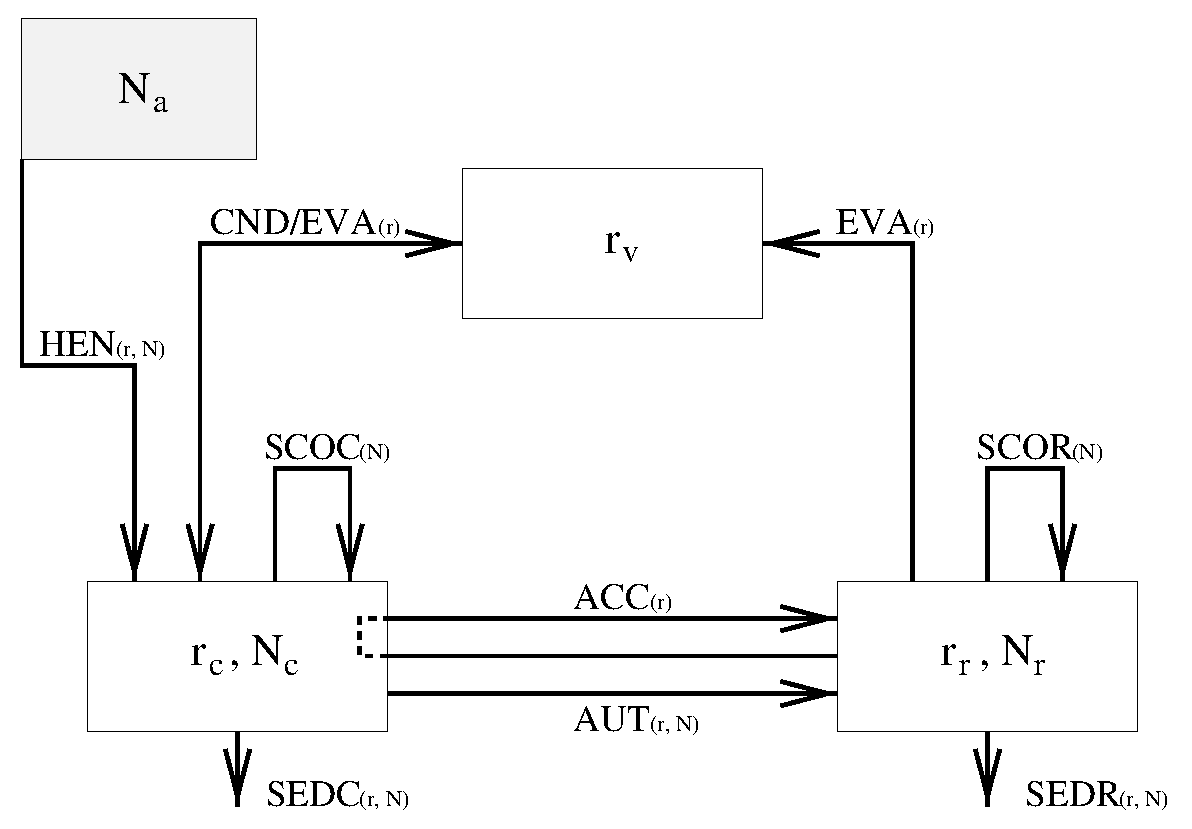
\includegraphics[width=10cm]{\EPSDIR/diagramC2R2.eps}}
\caption{Warm microphysical processes included in the C2R2 scheme (see text for
the acronyms and explanations).}
\label{diagramC2R2fig}
\end{figure}

\begin{table}
\caption{Nomenclature of the microphysical processes involved in (\ref{CONSTN1}a-d).}\label{tabnomen}
\begin{center}
\begin{tabular}{|c|c|c|c|c|}
\hline
%% & & & & \\
Symbols & Mechanisms & Sinks & Sources & Processes \\
\hline \hline
$RVHENC$ & $r_v\ \Longrightarrow \ r_c$ & $r_v$ & $r_c$ & nucleation \\
%% & & & & \\
$CVHENC$ & $N_n\ \Longrightarrow \ N_a$ & $N_n$ & $N_a$ & (implicitly) \\
         & $N_a\ \Longrightarrow \ N_c$ & $N_a$ & $N_c$ & \\
\hline
$RVCONC$ & $r_v\ \Longrightarrow \ r_c$ & $r_v$ & $r_c$ & condensation \\
         & $r_v\ \Longleftarrow \ r_c$ & $r_c$ & $r_v$ & {\&} evaporation \\
\hline
$RCAUTR$ & $r_c+r_c\ \Longrightarrow \ r_r$ & $r_c$ & $r_r$ & autoconversion \\
%% & & & & \\
$CCAUTR$ & $N_c+N_c\ \Longrightarrow \ N_r$ & $N_c$ & $N_r$ & \\
\hline
$RCACCR$ & $r_c+r_r\ \Longrightarrow \ r_r$ & $r_c$ & $r_r$ & accretion \\
%% & & & & \\
$CCACCR$ & $N_c+N_c\ \Longrightarrow \ N_r$ & $N_c$ & $N_r$ & \\
\hline
$RREVAV$ & $r_r\ \Longrightarrow \ r_v$ & $r_r$ & $r_v$ & evaporation \\
\hline
$CRSCOR$ & $N_r+N_r\ \Longrightarrow \ N_r$ & $N_r$ & $N_r$  & self-collection \\ 
%% & & & & break-up \\
$CCSCOC$ & $N_c+N_c\ \Longrightarrow \ N_c$ & $N_c$ & $N_c$  & {\&} break-up \\
\hline
$RSEDR$ & $r_r\ \Longrightarrow \ r_r$ & $r_r$ & $r_r$ & sedimentation \\
%% & & & & \\
$CSEDR$ & $N_r\ \Longrightarrow \ N_r$ & $N_r$ & $N_r$ & \\
\hline
\end{tabular}
\end{center}
\end{table}

\subsubsection{CCN activation (CVHENC) and reversible condensation/evaporation
of droplets (RVCONC)}

The CCN activation  and the condensation growth of cloud droplets are the 
dominant processes affecting distinctly the number concentration ($N_c$) 
and the mixing ratio ($r_c$) of cloud liquid water at the early stage of 
the cloud lifetime. These processes are difficult to model explicitly 
because they depend upon the maximum (CCN activation) and mean (condensation) 
local supersaturation values $s_{v,w}$ in contact with the CCN and the 
droplets. This quantity is not generally well captured in cloud models 
because its scale is highly variable and because the activation process results 
from an unstable thermodynamical equilibrium at short timescales in 
competition with the condensation growth that just tends to absorb any 
excess of supersaturation.

The parameterization of the CCN activation follows the diagnostic and 
integral approach of Twomey (1959) as improved by Cohard et al. (1998) 
where CCN activation spectra are expressed in the following functional 
form:
%
\beq\label{CCNSPEC}
N_{CCN}= C s_{{v,w}}^k F(\mu,\frac{\displaystyle{k}}{\displaystyle{2}},
		  \frac{\displaystyle{k}}{\displaystyle{2}}+1;-\beta s_{{v,w}}^2).
\eeq
%
\noindent $F(a,b,c;x)$ is the hypergeometric function. This form 
adheres more closely to observations of $N_{CCN}$ at large $s_{v,w}$ 
($N_{CCN}$ is finite as $s_{{v,w}}$ goes to infinity) as compared
to the traditional $C s_{{v,w}}^k$ law. Furthermore Cohard et al. (2000c)
show that it is possible to establish parametric relations between the four 
unknowns in (\ref{CCNSPEC}) and characteristics of lognormal distributions
of underlying aerosols with variable chemical composition and solubility.
Thus the $k$, $\beta$ and $\mu$ parameters of
(\ref{CCNSPEC}) can be expressed with the following formulas:
\begin{subequations}\label{SYS2}
\begin{align}
\frac{k}{k_0} & = \Big(\frac{{\rm ln}(\sigma)}{{\rm ln}(\sigma)_0}\Big)^{\alpha_k^{\sigma}},
  \tag{\ref{SYS2}a} \\
\frac{{\beta}}{{\beta}_0} & =
        \Big(\frac{\overline{r}}{\overline{r}_0}\Big)^{\alpha_{\beta}^{\overline{r}}}
    \exp\Big({\raisebox{-0.75ex}{${}^{\alpha_{\beta}^{\sigma}}$}}(\frac{{\rm ln}(\sigma)}{{\rm ln}(\sigma)_0}-1)\Big)
        \Big(\frac{\epsilon_m}{{\epsilon_m}_0}\Big)^{\alpha_{\beta}^{\epsilon_m}}
        \Big(\frac{T}{T_0}\Big)^{\alpha_{\beta}^{T}},
  \tag{\ref{SYS2}b} \\
\frac{{\mu}}{{\mu}_0} & = \Big(\frac{{\rm ln}(\sigma)}{{\rm ln}(\sigma)_0}\Big)^{\alpha_{\mu}^{\sigma}}.
  \tag{\ref{SYS2}c}
\end{align}
\end{subequations}
\addtocounter{equation}{1}
%
\noindent The values of the new coefficients in (\ref{SYS2}a-c) can be taken
from Tables 2 and 3 of Cohard et al. (2000c). The remaining parameter $C$ in
(\ref{CCNSPEC}) is deduced from the total CCN number concentration
($N_{CCN}^{max}$) using
%
\begin{align}
\label{CCNLIM1}
\displaystyle{\lim_{s_{v,w} \rightarrow +\infty}}
N_{CCN}(s_{v,w}) = N_{CCN}^{max} =
  \frac{\displaystyle{C}}{\displaystyle{\beta ^{k/2}}}
   \frac{\displaystyle{\Gamma(k/2 + 1)\Gamma(\mu- k/2)}}
   {\displaystyle{\Gamma(\mu)}}
\end{align}
\addtocounter{equation}{1}
%
\noindent under the condition that $k$ verifies $k<2\mu$ which is always
satisfied here.

Using (\ref{CCNSPEC}) and following Twomey's method, Cohard et al. (1998)
showed that an estimate of the maximum supersaturation $s_{{v,w}_{MAX}}$
is the root of
\beq\label{MAJORS}
s^{k+2}_{{v,w}_{MAX}}F(\mu,\frac{k}{2},\frac{k}{2}+\frac
{3}{2},-\beta s^{2}_{{v,w}_{MAX}})=\frac{\rho_a(\psi_1w)^{3/2}}{2kC\pi\rho_w\psi_2
(G)^{3/2}B(\frac{\displaystyle k}{\displaystyle 2},\frac{\displaystyle 3}
{\displaystyle 2})}.
\eeq
\noindent Substituting values of $s_{v,w}=s_{{v,w}_{MAX}}$ into (\ref{CCNSPEC})
provides an estimate of the potentially activable CCN number concentration, 
so the production rate of newly nucleated droplets is given by comparison 
with CCN that have been already activated. It is also worth to note that
(\ref{CCNSPEC}) and (\ref{MAJORS}) can be easily generalized to a mixture 
of aerosols.

The reversible condensation/evaporation process is treated implicitly 
as a result of a non-iterative vapor saturation adjustment (see Cohard
and Pinty, 2000a).  This treatment is well justified by observations 
that show that the interior of clouds is nearly in thermodynamical equilibrium
($s_{v,w}<1 \%$). The condensation rate is obtained after solving for $T$ 
the equation of the first law of thermodynamics,
\beq\label{THCON}
(T-T^*) + {L_v(T) \over C_{ph}} (r_{vs}(T)-r_v^*) = 0
\eeq
\noindent where $T^*$ and $r_v^*$ are the temperature and vapor mixing 
ratio of an intermediate state after integrating all the other explicit 
processes. $r_{vs}(T)$ is the saturated water vapor mixing ratio, $L_v(T)$ 
the latent heat of vaporization and $C_{ph}$ the heat capacity of cloudy air. 
The condensation rate is given by
\beq\label{RCCON}
RVCONC = max(-r_c, r_v^* - r_{vs}(T))/\delta t
\eeq

\subsubsection{Coalescence}

A short analysis of the stochastic collection equation indicates that bulk 
microphysical schemes always need a 
parameterization for the autoconversion terms (formation of raindrops by droplet
coalescence) while the other processes (including raindrop growth by accretion 
and self-collection) can be treated analytically using the collection kernels 
of Long (1974).

\paragraph{Autoconversion (RCAUTR and CCAUTR)}

The parameterization relies on the work of Berry and Reinhardt (1974) for 
the computation of the RCAUTR term. The parameterization is built on the 
observation that a characteristic water content $L$ of small drops develops 
steadily over a characteristic timescale $\tau$. These two positive 
quantities are expressed in the ranges 20 $\mu$m $\leq D_c \leq$ 36 $\mu$m 
and 0 $\leq \nu_c \leq$ 3 by:
%
\begin{subequations} \label{BERRY}
\begin{align}
L=&2.7 \times 10^{-2}\rho_a r_c
(\dfrac{1}{16}\times 10^{20}\sigma_c^3D_c-0.4) \tag{\ref{BERRY}a}\\
\tau=& 3.7\frac{\displaystyle{1}}{\displaystyle{\rho_a r_c}}
(0.5 \times 10^6\sigma_c-7.5)^{-1} \tag{\ref{BERRY}b}
\end{align}
\end{subequations}
\addtocounter{equation}{1}
%
\noindent where the mean-volume drop diameter $D_c$ and the standard 
deviation $\sigma_c$ are computed using (\ref{MOMENT}). Eqs({\ref{BERRY}a})
and ({\ref{BERRY}b}) are combined to get: 
%
\begin{align}
\label{RCAUT}
RCAUTR = & - max(\frac{\displaystyle{L}}{\displaystyle{\tau}},0.)
\end{align}
%

A suitable parameterization of the CCAUTR rate is more difficult to obtain
because the original Berry and Reinhardt's parameterization tends to 
accumulate the freshly formed drops by autoconversion in the lowest
part of the raindrop spectrum thus preventing the development of sizeable
raindrops. This led Cohard and Pinty (2000a) to the conclusion that it is 
important to restrict the original Berry and Reinhardt formulation:
%
\begin{align}
\label{NCAUT}
CCAUTR = & -3.5 \times 10^9 \;\frac{\displaystyle{\rho_a L}}{\displaystyle{\tau}}
\end{align}
%
\noindent to situations where $D_r<D_h$ where $D_h$ is the "hump diameter"
defined by Berry and Reinhardt (1974). For cases where $D_r>D_h$, it is
assumed that the autoconversion of the cloud droplets does not modify the 
mean-volume diameter so (\ref{NCAUT}) is replaced by:
%
\beq\label{NCCAUTR}
CCAUTR = \frac{\displaystyle{N_r}}{\displaystyle{r_r}} RCAUTR
\eeq
%

\paragraph{Accretion (RCACCR and CCACCR) and self-collections (CCSCOC 
and CRSCOR)}

The processes of accretion and self-collections associated to polynomial 
collection kernels, can be integrated analytically in bulk schemes as 
shown by Cohard and Pinty (2000a). The collection kernels of Long (1974), 
already used by Ziegler (1985), are considered in this study:
%
\beq\label{LONG}
K(D_1,D_2) =
  \begin{cases}
K_2  (D_1^6+D_2^6) & \text{if $D_1\leq 100 \mu$m}, \\
K_1  (D_1^3+D_2^3) & \text{if $D_1 > 100 \mu$m}. \\
  \end{cases}
\eeq
%
\noindent with $K_2=2.59 \times 10^{15}$ m$^{-3}$s$^{-1}$ and 
$K_1=3.03 \times 10^3$ s$^{-1}$. As recommended by Berry and Reinhardt (1974), 
the accretion and the self-collection of raindrops are accounted for once 
$r_r>1.2\times L/\rho_a$. The cumbersome expressions of the different ACC and 
SCO terms have been obtained by Cohard and Pinty (2000a) for the raindrops:
%                                       
\beq\label{ACCR1}
\begin{array}{rl}
{\rm If}\; D_r \geq 100 \mu{\rm m} & \\
CCACCR & = -K_1 N_cN_r                
\Big(\frac{\displaystyle{ \Gamma(\nu_c+3/\alpha_c)}}
{\displaystyle{\Gamma(\nu_c)\lambda_c^3}}+
\frac{\displaystyle{\Gamma(\nu_r+3/\alpha_r)}}
{\displaystyle{\Gamma(\nu_r)\lambda_r^3}}\Big)\\
\\                                      
RCACCR & = -\frac{\displaystyle{\pi}}{\displaystyle{6}}
\frac{\displaystyle{\rho_w}}{\displaystyle{\rho_{a}}} K_1
\frac{ \displaystyle{N_cN_r}}{\displaystyle{\lambda_c^3}}
\Big(\frac{\displaystyle{\Gamma(\nu_c+6/\alpha_c) }}
{\displaystyle{\Gamma(\nu_c)\lambda_c^3}} +
\frac{\displaystyle{\Gamma(\nu_c+3/\alpha_c)}}
{\displaystyle{\Gamma(\nu_c)}}          
\frac{\displaystyle{\Gamma(\nu_r+3/\alpha_r)}}
{\displaystyle{\Gamma(\nu_r)\lambda_r^3}}\Big)\\
\\
CRSCOR & = - K_1 N_r^2 \frac{\displaystyle{\Gamma(\nu_r+3/\alpha_r)}}
                            {\displaystyle{\Gamma(\nu_r)\lambda_r^{3}}}
\end{array}                             
\eeq                                    
%

%
\beq\label{ACCR2}
\begin{array}{rl}
{\rm If}\; D_r < 100 \mu{\rm m} & \\
CCACCR & = -K_2 N_cN_r
\Big(\frac{\displaystyle{ \Gamma(\nu_c+6/\alpha_c)}}
{\displaystyle{\Gamma(\nu_c)\lambda_c^6}}+
\frac{\displaystyle{\Gamma(\nu_r+6/\alpha_r)}}
{\displaystyle{\Gamma(\nu_r)\lambda_r^6}}\Big)\\
\\
RCACCR & = -\frac{\displaystyle{\pi}}{\displaystyle{6}}
\frac{\displaystyle{\rho_w}}{\displaystyle{\rho_{a}}} K_2
\frac{ \displaystyle{N_cN_r}}{\displaystyle{\lambda_c^3}}
\Big(\frac{\displaystyle{\Gamma(\nu_c+9/\alpha_c) }}
{\displaystyle{\Gamma(\nu_c)\lambda_c^6}} +
\frac{\displaystyle{\Gamma(\nu_c+3/\alpha_c)}}
{\displaystyle{\Gamma(\nu_c)}}
\frac{\displaystyle{\Gamma(\nu_r+6/\alpha_r)}}
{\displaystyle{\Gamma(\nu_r)\lambda_r^6}}\Big)\\
\\
CRSCOR & = - K_2 N_r^2 \frac{\displaystyle{\Gamma(\nu_r+6/\alpha_r)}}
                            {\displaystyle{\Gamma(\nu_r)\lambda_r^{6}}}
\end{array}
\eeq
%

and for the cloud droplets
%
\beq\label{SCOC}
\begin{array}{rl}
%{\rm as}\; D_c < 100 \mu{\rm m} & \\
CCSCOC & = - K_1 N_c^2 \frac{\displaystyle{\Gamma(\nu_c+3/\alpha_c)}}
                            {\displaystyle{\Gamma(\nu_c)\lambda_c^{3}}}
\end{array}
\eeq
%

\subsubsection{Break-up}

Break-up is an efficient process acting on the concentration of the large 
drops (a key role to explain the high reflectivity core of the tropical rainband
in the present case study). 

Firstly, collisional break-up is introduced as in Verlinde and 
Cotton (1993), where a bulk collection efficiency $E_c<1$ is used to damp 
the growth of the raindrops by self-collection. In the scheme, the 
preceeding $CRSCOR$ term is multiplied by the $E_c$ factor with the 
following definition:
%
\beq\label{BRUP}
E_c=
  \begin{cases}
1 
  &\text{if $D_r<600 \mu{\rm m}$}, \\
\exp(-2.5 \times 10^{3}(D_r-6 \times 10^{-4}))
  &\text{if $600 \mu{\rm m}\leq D_r<2000 \mu{\rm m}$},\\
0 
  &\text{if $D_r\geq 2000 \mu{\rm m}$}.
  \end{cases}
\eeq
%
\noindent Values of the cutoff diameters in (\ref{BRUP}) have been subjected 
to a specific evaluation in Cohard and Pinty (2000b). 

Secondly and as discussed by Cohard and Pinty (2000b), the inclusion of 
an additional drop size limiter (a substitute for a spontaneous break-up 
parameterization) is necessary to remove the giant drops that can be 
produced spuriously by an unaccurate differential transport of $r_r$ and 
$N_r$ (advection and sedimentation terms). The correction is applied 
whenever $D_r$ is larger than 3000 $\mu$m so beyond the range of active
collisional break-up (see Cohard and Pinty (2000b) for further details).

\subsubsection{Evaporation (RREVAV)}

The evaporation rate of a raindrop population, falling in an undersaturated 
environment ($s_{v,w} \ll 0$) is obtained after performing an analytical 
integration over the whole drop mass spectrum. The size evolution of a single 
evaporating drop of diameter $D$ is given by
%
\beq\label{EVAP1}
   \frac{\displaystyle{d D}}{\displaystyle{d t}} \Big|_{EVA}
 = \frac{\displaystyle{4 s_{v,w} \bar f G}}{\displaystyle{D}}
\eeq
%
\noindent where the ventilation factor $\bar f$, an empirical function of the Reynolds
number $Re=VD/\nu_{cin}$ of the flow, is given by:
%
\beq\label{EVAP2}
\begin{array}{rl}
\bar f &= 0.78 + F Re ^{0.5}
= 0.78 + 0.265\Big[ \Big( \frac{\displaystyle{\rho_{00}}}{\displaystyle{\rho_{a}}} \Big)^{0.4}
                      \frac{\displaystyle{cD^{d+1}}}{\displaystyle{\nu_{cin}}} \Big]^{0.5}\\
\end{array}
\eeq
%
\noindent after inserting (\ref{TERMVEL}). Integrating (\ref{EVAP1}) with (\ref{EVAP2})
and (\ref{GAMMA}) leads to an analytical expression of the evaporation rate that is:
\begin{align}
\label{EVAP3}
RREVAV &= \frac{\displaystyle{1}}{\displaystyle{\rho_{a}}}
\displaystyle{\int_0^{+\infty} 
\frac{\displaystyle{\pi}}{\displaystyle{2}} \rho_w D^2 
\frac{\displaystyle{d D}}{\displaystyle{d t}} \Big|_{EVA} n_r(D) dD }\\
&=\frac{\displaystyle{2 \pi s_{v,w} N_r G}}{\displaystyle{\lambda \Gamma(\lambda)}}
  \frac{\displaystyle{\rho_w}}{\displaystyle{\rho_{a}}}
\Big[ 0.78
+ 0.265 \Big( \frac{\displaystyle{\rho_{00}}}{\displaystyle{\rho_{a}}} \Big)^{0.2} 
    \Big( \frac{\displaystyle{c}}{\displaystyle{\nu_{cin}}}        \Big)^{0.5}
          \frac{\displaystyle{\Gamma (\nu_r+(d+3)/2\alpha_r)}}
	       {\displaystyle{\lambda_r^{(d+1)/2}}} \Big]. \notag
\end{align}
\addtocounter{equation}{1}
Concentrations $N_r$ are not affected by evaporation in the present scheme. 
However if the mean volume drop diameter becomes smaller than 82~$\mu$m 
(the hypothetical size separation between the droplet and drop modes)
then all raindrops are converted into cloud droplets, i.e. $N_c = N_c + N_r; 
r_c = r_c + r_r$ and $N_r = r_r = 0.$ 

\subsubsection{Sedimentation (RSEDR and CSEDR)}

Due to the fact that the terminal velocity of drops depends on their size,
the gravitational sedimentation of hydrometeors is selective if one considers 
the whole range of raindrop spectra. This leads to an efficient size sorting 
phenomenom which is important in the case of warm cumuli where some drops 
can be large enough to fall while smaller ones are delayed and maintained 
in updraft cores for further growth. This differential settling between drops 
is accounted for in two-moment schemes because both sedimentation
fluxes of $N_r$ and $r_r$ are computed:
%\begin{align}
%\label{SEDIM1}
%RSEDR &= \frac{\displaystyle{1}}{\displaystyle{\rho_{a}}}
%\frac{\displaystyle{\partial}}{\displaystyle{\partial z}}
%\displaystyle{\int_0^\infty
%\frac{\pi}{6} \rho_w D^3 V(D) N(D) dD}  \notag \\
%      &= \frac{\displaystyle{1}}{\displaystyle{\rho_{a}}}
%\frac{\displaystyle{\partial}}{\displaystyle{\partial z}}
%\Big[c \big( \frac{\displaystyle{\rho_{00}}}{\displaystyle{\rho_{a}}}\big)
%^{0.4} \rho_{a} r_r
%\frac{\displaystyle{\Gamma(\nu_r+(d+3)/ \alpha_r)}}{\displaystyle{
%\lambda_r^{d}\Gamma(\nu_r+3/ \alpha_r)}}  \Big], \\
%\label{SEDIM2}
%CSEDR &= \frac{\displaystyle{\partial}}{\displaystyle{\partial z}}
%\displaystyle{\int_0^\infty V(D)N(D) dD} \notag \\
%      &= \frac{\displaystyle{\partial}}{\displaystyle{\partial z}}
%\Big[c \big( \frac{\displaystyle{\rho_{00}}}{\displaystyle{\rho_{a}}}\big)
%^{0.4} N_r
%\frac{\displaystyle{\Gamma(\nu_r +d/\alpha_r)}}
%{\displaystyle{\lambda_r^d \Gamma(\nu_r)}}\Big].
%\end{align}
\begin{align}
\label{SEDIM1}
RSEDR &= \frac{\displaystyle{1}}{\displaystyle{\rho_{a}}}
\frac{\displaystyle{\partial}}{\displaystyle{\partial z}}
\displaystyle{\int_0^\infty
\frac{\pi}{6} \rho_w D^3 V(D) n_r(D) dD} \notag \\
      &= \frac{\displaystyle{1}}{\displaystyle{\rho_{a}}}
\frac{\displaystyle{\partial}}{\displaystyle{\partial z}}
\Big[c \big( \frac{\displaystyle{\rho_{00}}}{\displaystyle{\rho_{a}}}\big)
^{0.4} \rho_{a} r_r
\frac{\displaystyle{\Gamma(\nu_r+(d+3)/ \alpha_r)}}{\displaystyle{
\lambda_r^{d}\Gamma(\nu_r+3/ \alpha_r)}}  \Big], \\
\label{SEDIM2}
CSEDR &= \frac{\displaystyle{\partial}}{\displaystyle{\partial z}}
\displaystyle{\int_0^\infty V(D) n_r(D) dD} 
       = \frac{\displaystyle{\partial}}{\displaystyle{\partial z}}
\Big[c \big( \frac{\displaystyle{\rho_{00}}}{\displaystyle{\rho_{a}}}\big)
^{0.4} N_r
\frac{\displaystyle{\Gamma(\nu_r +d/\alpha_r)}}
{\displaystyle{\lambda_r^d \Gamma(\nu_r)}}\Big].
\end{align}
In (\ref{SEDIM1})-(\ref{SEDIM2}), a simple power law dependence in diameter including air
density effect (Foote and Du Toit 1969) has been assumed:
\beq\label{TERMVEL}
V(D)= \Big( \frac{\displaystyle{\rho_{00}}}{\displaystyle{\rho_{a}}}\Big)^{0.4} cD^d,
\eeq


\subsection*{Appendix: List of symbols}
\setlongtables
\begin{longtable}{ll}
$A$&$=4\sigma_{w/a}/R_v T\rho_w$\\
$B(a,b)$&beta function\\
$c$ and $d$&parameters of the fall speed-diameter relationship for the\\
           &water drops\\
$C$&activation spectrum coefficient\\
$C_{vv}$&heat capacity at constant volume of water vapor\\
$C_{pd}$, $C_{pv}$ and $C_{w}$&heat capacity at constant pressure of dry air, water vapor\\
                              &and liquid water\\
$C_{ph}$&$=C_{pd}+r_v C_{pv}+(r_c+r_r)C_{w}$\\
$D$, $D_1$ and $D_2$&drop diameters\\
$D_c$, $D_r$&mean volume drop diameter for cloud droplet and raindrop\\
            &distributions\\
%% $D_{crit}$&critical diameter of newly nucleated droplets\\
$D_v$&diffusivity of water vapor in the air\\
$e_v$&water vapor pressure\\
$e_{vs}$&saturation vapor pressure over water\\
$E_c$&collection efficiency\\
$\bar f$&ventilation factor\\
$F$&ventilation coefficient\\
$F(a,b,c;x)$&hypergeometric function\\
$G(D,T,P)$&$=\displaystyle{{1 \over \rho_w}\Big({R_v T \over e_{vs}(T) D_v} +
{L_v(T) \over k_a T}({L_v(T) \over R_v T} -1)\Big)^{-1}}$\\
$k$ and $k_0$&activation spectrum coefficients\\
$k_a$&heat conductivity of air\\
$K(x,y)$ and $K(D_1,D_2)$&collection kernels\\
$K_1$ and $K_2$&Long's collection kernel coefficients\\
$L$&autoconversion water mass\\
$L_v$&latent heat of vaporization\\
$n$, $n_c$ and $n_r$&total, cloud droplet and raindrop size distributions\\
$N_0$&intercept parameter of an exponential distribution law\\
$N_c$, $N_r$&cloud droplet and raindrop number concentration\\
$N_n$, $N_a$&condensation nuclei and activated CCN number concentration\\
$N_{CCN}$&total activable CCN number concentration\\
$M_w$&molar weight of water\\
$M_i(p)$&$p$\_moment of the $i$\_drop size distribution\\
$P$ and $P_{00}$&pressure and reference pressure (1000 hPa)\\
$\overline{r}$&geometric mean radius of the CCN lognormal distribution\\
$r_v$, $r_c$ and $r_r$&water vapor, cloud water and rain water mixing ratios\\
$r_{vs}$&saturated vapor mixing ratio\\
$R_d$ and $R_v$&gas constant for dry air and water vapor\\
$Re$&Reynolds number\\
$s_{v,w}$&supersaturation ($=e_v/e_{vs}-1$)\\
$s_{{v,w}_{MAX}}$&maximum supersaturation\\
$t$&time\\
$T$ and $T_{00}$&temperature and reference temperature (273.16 K)\\
$V(D)$&drop fall speed of diameter $D$\\
$w$&updraft velocity\\
$x$ and $y$&drop mass\\
$z$&height or vertical coordinate\\
$\alpha_{\{k, \beta, \mu\}}^{\{{\overline r}, {\rm ln}(\sigma), \epsilon_m, T\}}$&adjusted parameters defining the CCN spectrum coefficients\\
$\alpha_c$, $\alpha_r$&dispersion parameter of the generalized gamma distribution\\
                      &law for the cloud droplets and the raindrops\\
$\beta$ and ${\beta}_0$&activation spectrum coefficient\\
$\delta t$&time step\\
$\Gamma(a)$&complete gamma function\\
$\epsilon$&$=R_v/R_d$\\
$\epsilon_m$&aerosol soluble fraction\\
$\theta$&potential temperature\\
$\lambda_c$, $\lambda_r$&slope parameter of the generalized gamma distribution law\\
                        &for the cloud droplets and the raindrops\\
$\mu$ and ${\mu}_0$&activation spectrum coefficients\\
$\nu_c$, $\nu_r$&dispersion parameter of the generalized gamma distribution\\
                &law for the cloud droplets and the raindrops\\
$\nu_{cin}$&kinematic viscosity of air\\
$\Pi$&=$(P/P_{00})^{R_d/C_{pd}}$\\
$\rho_a$ and $\rho_w$&air and liquid water densities\\
$\rho_{00}$&air density at $P=P_{00}$ and $T=T_{00}$\\
$\sigma$&geometric standard deviation of the CCN lognormal distribution\\
$\sigma_c$&standard deviation of cloud droplet distribution\\
$\sigma_{w/a}$&surface tension of water over the air\\
$\tau$&timescale for autoconversion\\
$\psi_1(T,P)$&$=\displaystyle{\frac{g}{TR_d}}\displaystyle{\Big(\frac{L_v}{c_pT}-1
\Big)}$ \\
$\psi_2(T,P)$&$=\displaystyle{\Big(\frac{P}{\epsilon e_{vs}(T)}+
\frac{\epsilon L_v^2} {R_dT^2c_p}} \Big)$\\
\end{longtable}

%
\section{The two-moment microphysical scheme for LES of stratocumulus}\label{KHKO}
\subsection{Introduction}
%

The KHKO scheme is a 2-moment microphysical scheme specially designed for boundary layer clouds. These clouds are low precipitating warm clouds, and not sufficiently thick to produce heavy rain. The precipitating hydrometeors are drizzle only: their diameter are of the order of several dozens of micrometers. The conversion rates that impact drizzle formation and evolution are parameterized according to Khairoutdinov and Kogan (2000) (KK00) microphysical scheme. These processes are autoconversion, accretion, drizzle sedimentation and drizzle evaporation. Microphysical processes that impact cloud formation are parameterized as in the C2R2 scheme: cloud droplet condensation and evaporation follow Langlois (1973) and activation follows Cohard et al. (1998) (see the C2R2 scientific documentation). Moreover cloud droplet sedimentation is resolved by assuming a Stokes flow to calculate the cloud droplets terminal velocity and an analytical distribution to describe the cloud droplet spectra as in the C2R2 scheme.
Microphysical prognostic variables are the same as in the C2R2 scheme: cloud droplet number concentration $N_{c}$ and mixing ratio $r_{c}$, precipitating hydrometeors number concentration $N_{r}$ and mixing ratio $r_{r}$, activated cloud condensation nuclei number concentration $N_{a}$.


The next section describes KK00 (the original scheme of Khairoutdinov and Kogan (2000)) and  KHKO (the corresponding scheme implemented in Meso-NH) specificities and limits.

\subsection{KK00 scheme specifities}


The KK00 scheme is a 2-moment bulk microphysical scheme. All processes are parameterized only as a function of mixing ratios and number concentrations of each category (cloud droplet and drizzle). 
The methodology developed in KK00 consisted to assume firstly a power law relationship between conversion rate and the prognostic variables. Each power law introduces coefficients that have to be determined. These coefficients have been empirically adjusted by using about 100 000 hydrometeors spectra obtained from four 3-D LES simulations of stratocumulus clouds using an explicit (bin) microphysical model. For each of these spectra, autoconversion and accretion conversion rates are calculated by integrating the stochastic collection equation. Then the coefficients in the parameterized expressions are evaluated by regression analysis.

Figure~\ref{figKHKO}a shows the range of cloud droplet mixing ratios and number concentrations of spectra used to evaluate conversion rates. These values are typical of values encountered in stratocumulus as shown in Fig~\ref{figKHKO}b and Fig~\ref{figKHKO}c that represent cloud droplet mixing ratios and number concentrations of spectra measured respectively during the ACE-1 and 
ACE-2 field experiments. The advantage of adjusting coefficients using spectra simulated with an explicit model is that these spectra are representative of boundary layer clouds realistic distributions.

\begin{figure}[!ht]
\centerline{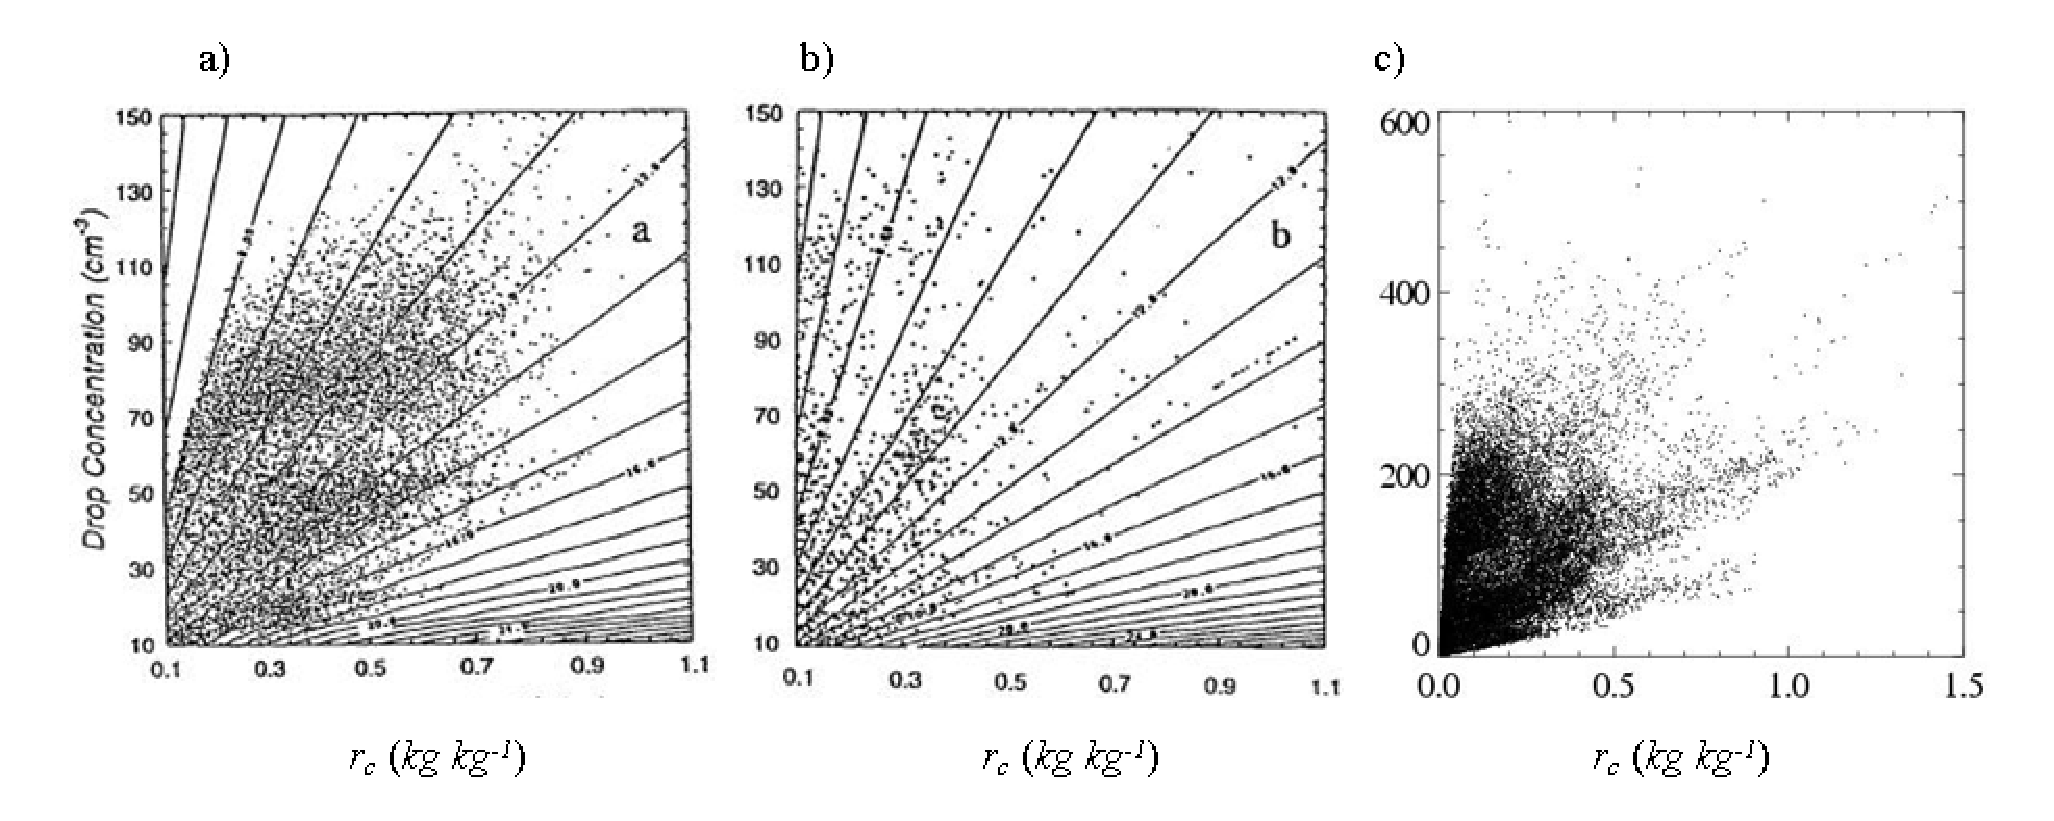
\includegraphics[width=\textwidth]{\EPSDIR/fig_khko1.eps}}
\caption{ a) A scatterplot of the parameter space used to evaluate the coefficients of the KK00  microphysical processes parameterizations. Each data point represents the cloud droplet mixing ratio and the number concentration calculated from an individual hydrometeor size spectrum simulated by the explicit microphysical model.
b) Similar to a) but for the spectra averaged over each aircraft flight leg in stratocumulus cloud during the first phase of ACE-1,
(following Khairoutdinov et Kogan (2000)),
c) Similar to a) but for the ensemble of spectra measured during ACE-2 field experiments (8 flights). Each spectra is averaged with a resolution of about 100~m horizontally. Note that different scales are used for this plot.}
\label{figKHKO} 
\end{figure}


Note that a value for $r_c$ of $1.1$~g~kg$^{-1}$ (the maximum value in Fig.~\ref{figKHKO}a) corresponds to an adiabatic cloud with a depth equal to about 550~m. This value can be calculated by assuming an adiabatic linear relationship between the mixing ratio at cloud top $r_c(H)$ and the cloud depth $H$ with an adiabatic coefficient $C_w$ equal to $2$ $10^{-6}$~kg~m$^{-4}$ : $r_c(H) = C_w H$. This scheme cannot be extended to deep convective clouds. 

In the KK00 scheme, separation between cloud droplets and drizzle is defined at a diameter $D_0$ equal to 50~$\mu$m. This low value permits consideration of drizzle in the precipitating category.

\noindent Parameterizations are expressed as a function of local microphysical values. Thus the scheme is valid only for simulations where microphysical fields are explicitly resolved i.e. in the LES configuration. Resolution must not be more than 200~m horizontally and a few ten of meters vertically (a vertical resolution of 10~m in the cloud is recommended).   


\subsection{System of equations}

For each prognostic variable, conservative equations in KHKO scheme are the following ones:


\begin{subequations} \label{SYSTKHKO}
\begin{align}
\frac{\displaystyle{\partial N_a}}{\displaystyle{\partial t}} =&
\sum \frac{\displaystyle{\partial N_a}}{\displaystyle{\partial t}} \Big|_{NMT}
+ \frac{\displaystyle{\partial N_a}}{\displaystyle{\partial t}} \Big|_{ACT}
+ \frac{\displaystyle{\partial N_a}}{\displaystyle{\partial t}} \Big|_{EVAPC} \tag{\ref{SYSTKHKO}a}\\
\frac{\displaystyle{\partial N_c}}{\displaystyle{\partial t}} =&
\sum \frac{\displaystyle{\partial N_c}}{\displaystyle{\partial t}} \Big|_{NMT}
+ \frac{\displaystyle{\partial N_c}}{\displaystyle{\partial t}} \Big|_{ACT} 
+ \frac{\displaystyle{\partial N_c}}{\displaystyle{\partial t}} \Big|_{SEDC} 
+ \frac{\displaystyle{\partial N_c}}{\displaystyle{\partial t}} \Big|_{AUTO} 
+ \frac{\displaystyle{\partial N_c}}{\displaystyle{\partial t}} \Big|_{ACCR}
+ \frac{\displaystyle{\partial N_c}}{\displaystyle{\partial t}} \Big|_{EVAPC}  \tag{\ref{SYSTKHKO}b}\\
\frac{\displaystyle{\partial r_c}}{\displaystyle{\partial t}} =&
\sum \frac{\displaystyle{\partial r_c}}{\displaystyle{\partial t}} \Big|_{NMT}
+ \frac{\displaystyle{\partial r_c}}{\displaystyle{\partial t}} \Big|_{ACT} 
+ \frac{\displaystyle{\partial r_c}}{\displaystyle{\partial t}} \Big|_{SEDC} 
+ \frac{\displaystyle{\partial r_c}}{\displaystyle{\partial t}} \Big|_{AUTO} 
+ \frac{\displaystyle{\partial r_c}}{\displaystyle{\partial t}} \Big|_{ACCR}
+ \frac{\displaystyle{\partial r_c}}{\displaystyle{\partial t}} \Big|_{CONDC}
+ \frac{\displaystyle{\partial r_c}}{\displaystyle{\partial t}} \Big|_{EVAPC} \tag{\ref{SYSTKHKO}c}\\
\frac{\displaystyle{\partial N_r}}{\displaystyle{\partial t}} =&
\sum \frac{\displaystyle{\partial N_r}}{\displaystyle{\partial t}} \Big|_{NMT}
+ \frac{\displaystyle{\partial N_r}}{\displaystyle{\partial t}} \Big|_{SEDR} 
+ \frac{\displaystyle{\partial N_r}}{\displaystyle{\partial t}} \Big|_{AUTO} 
+ \frac{\displaystyle{\partial N_r}}{\displaystyle{\partial t}} \Big|_{ACCR}
+ \frac{\displaystyle{\partial N_r}}{\displaystyle{\partial t}} \Big|_{EVAPR}   \tag{\ref{SYSTKHKO}d}\\
\frac{\displaystyle{\partial r_r}}{\displaystyle{\partial t}} =&
\sum \frac{\displaystyle{\partial r_r}}{\displaystyle{\partial t}} \Big|_{NMT}
+ \frac{\displaystyle{\partial r_r}}{\displaystyle{\partial t}} \Big|_{SEDR} 
+ \frac{\displaystyle{\partial r_r}}{\displaystyle{\partial t}} \Big|_{AUTO} 
+ \frac{\displaystyle{\partial r_r}}{\displaystyle{\partial t}} \Big|_{EVAPR} \tag{\ref{SYSTKHKO}e}
\end{align}
\end{subequations}
\addtocounter{equation}{1}



\noindent where the subscript $NMT$ refers to Non-Microphysical Tendencies (advection, turbulence, numerics and other physical processes), $ACT$, $SEDC$, $SEDR$, $AUTO$, $ACCR$, $CONDC$, $EVAPC$, $EVAPR$ are the microphysical contributions, i.e. respectively, activation, cloud droplet sedimentation, drizzle sedimentation, autoconversion, accretion, cloud droplet condensation, cloud droplet evaporation and drizzle evaporation. 

\noindent The KK00 scheme does not take into account the drizzle self-collection (on the contrary to C2R2 for raindrops): drizzle diameters are too low for this process to impact the drizzle number concentration $N_r$. Moreover in the KHKO scheme, water vapor condensation on precipitating hydrometeors is not taken into account (as in C2R2).

\noindent In order to close this system of equations the rhs terms are parameterized as a function of the prognostics variables. The next sections describe parameterizations of these processes except for cloud droplet condensation/evaporation and activation, that are identical to the C2R2 scheme. For a description of the latter the reader should refer to the C2R2 documentation.

\subsection{Collection processes}

\paragraph{Autoconversion}

Autoconversion is the process that initializes precipitating hydrometeor spectra. It depends on cloud droplet spectra characteristics. In the KK00 scheme it is assumed to depend on cloud droplets number concentration $N_c$ and mixing ratio $r_c$. After regression analysis on bin model simulations, KK00 obtain the following parameterized expressions for the mixing ratios conversion rates by autoconversion: 

\begin{equation}
\frac{\displaystyle{\partial r_r}}{\displaystyle{\partial t}} \Big|_{AUTO}=1350. r_c^{2.47}N_c^{-1.79}
\label{autoc}
\end{equation}

\begin{equation}
\frac{\displaystyle{\partial r_c}}{\displaystyle{\partial t}} \Big|_{AUTO}=
-\frac{\displaystyle{\partial r_r}}{\displaystyle{\partial t}} \Big|_{AUTO}
\end{equation}


\noindent The cloud droplet number concentration source term is evaluated by assuming that all collected cloud droplet diameters are equal to the mean volume diameter $D_c$:

\begin{equation}
\frac{\displaystyle{\partial N_c}}{\displaystyle{\partial t}} \Big|_{AUTO}=-
\frac{(\frac{\displaystyle{\partial r_r}}{\displaystyle{\partial t}}) \Big|_{AUTO}}
{\frac{\pi\rho_w}{6\rho_a}D_c^3}
\end{equation}


\noindent New drizzle drops are assumed to have the diameter $D_0$ equal to 50~$\mu$m. Thus the drizzle number concentration source term due to autoconversion is:

\begin{equation}
\frac{\displaystyle{\partial N_r}}{\displaystyle{\partial t}} \Big|_{AUTO}=
\frac{\frac{\displaystyle{\partial r_r}}{\displaystyle{\partial t}} \Big|_{AUTO}}
{\frac{\pi\rho_w}{6\rho_a}D_0^{3}}
\end{equation}

\subsubsection{Accretion}

Accretion rate has to be expressed as a function of cloud droplets spectra and precipitating hydrometeors spectra because accretion represents an interaction between the two categories. KK00 assume that accretion rate depends only on cloud droplet and drizzle mixing ratios. After regression analysis the following expressions for mixing ratios conversion rates are obtained: 

\begin{equation}
\frac{\displaystyle{\partial r_r}}{\displaystyle{\partial t}} \Big|_{ACCR}=
67(r_{c}r_{r})^{1.15}
\end{equation}
\begin{equation}
\frac{\displaystyle{\partial r_c}}{\displaystyle{\partial t}} \Big|_{ACCR}=
-\frac{\displaystyle{\partial r_r}}{\displaystyle{\partial t}} \Big|_{ACCR}
\end{equation}

\noindent Similar to autoconversion, cloud droplets number concentration accretion sink term is expressed as the following: 

\begin{equation}
\frac{\displaystyle{\partial N_c}}{\displaystyle{\partial t}} \Big|_{ACCR}=-
\frac{\frac{\displaystyle{\partial r_r}}{\displaystyle{\partial t}} \Big|_{ACCR}}
{\frac{\pi\rho_w}{6\rho_a}D_c^3}
\end{equation}

\noindent Cloud droplets collection by precipitating hydrometeors involves an increase of precipitating hydrometeors mass but not of their number. For that reason there is no accretion source term for the drizzle number concentration.


\subsection{Break-up}

Break-up is applied to achieve a numerical goal only. Drizzle drops are not large enough to take into account this process. However, at some grid point, the drizzle drops number concentration and mixing ratio have non-physical low values that can result in an inconsistency between these two values and thus overly large drizzle mean volume diameters. In order to avoid this divergence, break-up is applied to limit too low values of drizzle number concentration and keep consistency between the drizzle number concentration and mixing ratio.
The same protection is done for the cloud droplets number concentration. The latter is corrected when necessary in order that the cloud droplets mean volume diameter do not exceed the limit diameter between cloud droplets and drizzle i.e. 50~$\mu$m.

\subsection{Drizzle evaporation}

Precipitating drops evaporation rate can be expressed as:
\begin{equation}
\frac{\displaystyle{\partial r_r}}{\displaystyle{\partial t}} \Big|_{EVAPR}=
\frac{2\pi\rho_w}{\rho_a}G(T,P) s_{v,w}\int_{0}^{\infty}Dn_r(D)dD
\end{equation}


\noindent where $G(T,P)$ is a function of temperature and pressure, $n_r(D)$ is the drizzle density function 
and $s_{v,w}$ is the subsaturation ($s_{v,w}=e_v/e_{vs}-1$). 
Note that drizzle drops have a sufficiently low diameter to ignore the ventilation factor. 
By introducing a coefficient $C_{evap}$ equal to the ratio of the drizzle drop mean diameter to the drizzle drop mean volume diameter, it becomes:

\begin{equation}
\frac{\displaystyle{\partial r_r}}{\displaystyle{\partial t}} \Big|_{EVAPR}=
12C_{evap}G(T,P)(\frac{\pi\rho_w}{6\rho_a})^{\frac{2}{3}}r_r^{\frac{1}{3}}N_r^{\frac{2}{3}}s_{v,w}
\end{equation}

\noindent KK00 assume that $C_{evap}$ is a constant parameter. Its value has been adjusted using the spectra derived from the bin model simulations. They propose: $C_{evap}=0.86$. The uncertainty of this parameter is estimated on the order of $15-20\%$.

\noindent KK00 calculate the rate of change of drizzle number concentration as:

\begin{equation}
\frac{\displaystyle{\partial N_r}}{\displaystyle{\partial t}} \Big|_{EVAPR}=
\frac{N_r}{r_r}\frac{\frac{\displaystyle{\partial r_r}}{\displaystyle{\partial t}} \Big|_{EVAPR}}
{\frac{\pi\rho_w}{6\rho_a}D_r^3}
\end{equation}


\noindent Water vapor condensation on drizzle is not taken into account in the model. In the presence of cloud droplets, the amount of water vapor condensed on drizzle is negligible. Because positive supersaturation is encountered in clouds only, it is consistent to neglect condensation on drizzle.


\subsection{Sedimentation} 

\subsubsection{Generalities}

For the two categories of liquid water, number concentration and mixing ratio sedimentation rates  can be expressed respectively as function of the number concentration sedimentation flux $F_{N_i}$ (in m$^{-2}$ s$^{-1}$) and the mixing ratio sedimentation flux $F_{r_i}$ 
(in kg~m$^{-2}$ s$^{-1}$) with $i=[c, r]$.

\begin{equation}
\frac{\displaystyle{\partial N_i}}{\displaystyle{\partial t}} \Big|_{SED_i}=
\frac{\displaystyle{\partial F_{N_i}}}{\displaystyle{\partial z}}
\end{equation}

\begin{equation}
\frac{\displaystyle{\partial r_i}}{\displaystyle{\partial t}} \Big|_{SED_i}=
\frac{1}{\rho_a}\frac{\displaystyle{\partial F_{r_i}}}{\displaystyle{\partial z}}
\end{equation}

\noindent with : $F_{N_i}=V_{N_i}N_i$ and $F_{r_i}=V_{r_i}\rho_ar_i$,

\noindent and : 

\begin{equation}
V_{N_i}=\frac{F_{N_i}}{N_i}=\frac{\int_{0}^{\infty}v(D)n_i(D)dD}{\int_{0}^{\infty}n_i(D)dD}
\end{equation}

\begin{equation}
V_{r_i}=\frac{F_{r_i}}{\rho_ar_i}=\frac{\int_{0}^{\infty}\frac{\pi}{6}\rho_wD^3v(D)n_i(D)dD}{\int_{0}^{\infty}\frac{\pi}{6}\rho_wD^3n_i(D)dD}
\end{equation}


\noindent $V_{r_i}$ is an average weighted by the third momentum of the distribution. 
For a non-monodispersed distribution, the mean terminal velocity of the mixing ratio $V_{r_i}$ is different and greater than the mean terminal velocity of the hydrometeors $V_{N_i}$, because the flux of the hydrometeor mixing ratio is driven by hydrometeors of larger diameter.

\subsubsection{Drizzle sedimentation}

KK00 propose parameterized expressions of the velocity of the drizzle number concentration and the velocity of the mixing ratio as a function of the drizzle distribution mean volume diameter $D_r$:

\begin{equation}
V_{N_r}=0.0035D_r-0.1
\end{equation}
 
\begin{equation}
V_{r_r}=0.006D_r-0.2
\end{equation}


\noindent The coefficients have been tuned against the spectra simulated with the explicit model.

\subsubsection{Cloud droplets sedimentation}

KHKO introduces cloud droplet sedimentation on the contrary to 
KK00 parameterization, because this process has an impact on cloud evolution by reducing entrainment at cloud top (Ackerman et al. 2004; Bretherton et al. 2007). As in the C2R2 scheme, it is parameterized by assuming a Stokes law to calculate the cloud droplets terminal velocity and by assuming an analytical distribution to represent cloud droplet spectra. The analytical distribution used is a generalized gamma law (cf. C2R2 documentation). This law can be expressed as a function of $r_c$ and $N_c$ and two free parameters $\alpha_c$ and $\nu_c$. 

After integration, the sedimentation fluxes for the cloud droplet number concentration and the mixing ratio respectively are the following:

\begin{equation}
F_{N_c}=k_1N_cD_c^2\frac{\Gamma(\nu_c+\frac{2}{\alpha_c})}{\Gamma(\nu_c+\frac{3}{\alpha_c})^{\frac{2}{3}}}\Gamma(\nu_c)^{-\frac{1}{3}}
\end{equation}

\begin{equation}
F_{r_c}=k_2N_cD_c^5\frac{\Gamma(\nu_c+\frac{5}{\alpha_c})}{\Gamma(\nu_c+\frac{3}{\alpha_c})^{\frac{5}{3}}}\Gamma(\nu_c)^{\frac{2}{3}}
\end{equation}

\noindent where $\Gamma(x)$ is the gamma function and $\alpha_c=3$, $\nu_c=2$. These values have been adjusted by comparison with measured cloud droplet spectra during ACE-2 field campaign (Geoffroy 2007).




\subsection*{Appendix: List of symbols}
\setlongtables
\begin{longtable}{ll}

$C_{evap}$ &ratio of the drizzle drop mean radius \\
           &to the drizzle drop mean volume radius\\
$D_0$&separation between cloud droplets and drizzle (=$50$ $\mu$m)\\
$D_c$, $D_r$&mean volume drop diameter for cloud droplet and drizzle\\
            &distributions\\
$D_v$&diffusivity of water vapor in the air\\
$e_v$&water vapor pressure\\
$e_{vs}$&saturation vapor pressure over water\\
$F_{N_c}, F_{r_c}$&cloud number concentration and mixing ratio sedimentation flux\\
$F_{N_r}, F_{r_r}$&drizzle number concentration and mixing ratio sedimentation flux\\
$G(T,P)$&= $ =\frac{1}{\rho_w}(\frac{R_vT}{e_{vs}(T)D_v}+\frac{L_v(T)}{k_aT}(\frac{L_v(T)}{R_vT}-1))^{-1}$ \\
$k_a$&heat conductivity of air\\
$L_v$&latent heat of vaporisation\\
$n$, $n_c$ and $n_r$&total, cloud droplet and drizzle size distributions\\
$N_c$, $N_r$&cloud droplet and drizzle number concentration\\ 
$N_a$ &activated CCN number concentration\\
$P$ &pressure\\

$r_v$, $r_c$ and $r_r$&water vapor, cloud droplets and drizzle mixing ratios\\
$r_{vs}$&saturated water vapor mixing ratio\\
$R_v$&gaz constant for water vapor\\
$s_{v,w}$&supersaturation ($=e_v/e_{vs}-1$)\\
$T$&temperature\\
$v(D)$&Hydrometeor of diameter $D$ terminal velocity \\
$V_{N_r}, V_{r_r}$&drizzle number concentration and mixing ratio mean terminal velocity\\
$\alpha_c$, $\nu_c$&dispersion parameters of the generalized gamma distribution\\
                      &law for the cloud droplets distribution\\
$\rho_a$ and $\rho_w$&air and liquid water densities\\
$\Gamma(a)$&complete gamma function\\
\end{longtable}


\section{References}
\parindent 0truecm
\por
Berry, E. X., and R. L. Reinhardt, 1974: An analysis of cloud drop growth by
        collection: Part II. single initial distributions.
        {\it J. Atmos. Sci.},
        {\bf 31},
        1825-1831.
\por
Bretherton, C. S., P. N. Blossey, and J. Uchida, 2007: Cloud droplet sedimentation, entrainment efficiency,
           and subtropical stratocumulus albedo.
           {\it Geophys. Res. Lett.},
           {\bf 34,} 
           L03813
\por
Cohard, J.-M., J.-P. Pinty, and C. Bedos, 1998: Extending Twomey's analytical
        estimate of nucleated cloud droplet concentrations from CCN spectra.
        {\it J. Atmos. Sci.},
        {\bf 55,}
        3348-3357.
\por
Cohard, J.-M., and J.-P. Pinty, 2000a: A comprehensive two-moment warm
        microphysical bulk scheme. Part I: Description and selective tests.
        {\it Q. J. R. Meteorol. Soc.},
        {\bf 126},
        1815-1842.
\por
Cohard, J.-M., and J.-P. Pinty, 2000b: A comprehensive two-moment warm
        microphysical bulk scheme. Part I: 2D experiments with a
        non-hydrostatic model.
        {\it Q. J. R. Meteorol. Soc.},
        {\bf 126},
        1843-1859.
\por
Cohard, J.-M., J.-P. Pinty, and K. Suhre, 2000c: On the parameterization of
        activation spectra from CCN microphysical properties.
        {\it J. Geophys.  Res.},
        {\bf 105},
        D9,
        11753-11766.
\por
Foote, G. B., and P. S. Du Toit, 1969: Terminal velocity of raindrops aloft.
{\it J. Appl. Meteor.}, {\bf 8}, 249-253.
\por
Geleyn, J.-F., B. Catry, Y. Bouteloup, and R. Brozkova, 2008. A statistical approach for 
        sedimentation inside a micro-physical precipitation scheme.
        {\it Tellus},
        {\bf 60A},
        649-662.
\por
Geoffroy, O., 2007: Modelisation LES des precipitations dans les nuages de couche limite et parametrisation pour les GCM, Ph.D. thesis, Universite Paul Sabatier (Toulouse III).
\por
Kessler, E., 1969: On the distribution and continuity of water sustance in
atmospheric circulations. {\it Meteor. Monog.}, {\bf 10}, N$^\circ$ 32, 84pp.
\por
Khairoudinov, M., and Y. Kogan, 2000: A new cloud physics parameterization
        in a large-eddy simulation model of marine stratocumulus.
        {\it Mon. Wea. Rev.},
        {\bf 128,}
        229-243.
\por
Langlois, W.E., 1973: A rapidly convergent procedure for computing large-scale
condensation in a dynamical weather model. {\it Tellus}, {\bf 25}, 86-87.
\por
Long, A. B., 1974: Solutions to the droplet collection equation for polynomial
        kernels.
        {\it J. Atmos. Sci.},
        {\bf 31},
        1040-1057.
\por
Liu, J. Y, and H. D. Orville, 1969: Numerical modeling of precipitation and cloud
shadow effects on mountain-induced cumuli. {\it J. Atmos. Sci.}, {\bf 26},
1283-1298.
\por
Press, W. H., S. A. Teukolsky, W. T. Vetterling, and B. P. Flannery, 1992:
        {\it Numerical Recipes in FORTRAN: The Art of Scientific Computing.}
        2nd Ed.
        Cambridge University Press,
        963 pp.
\por
Pruppacher, H. R and J. D. Klett, 1978: Microphysics of clouds and precipitation.
Reidel, 714pp
\por
Rood, R. B., 1987: Numerical advection algorithms and their role in atmospheric
transport and chemistry models. {\it Review of Geoph.}, {\bf 25}, 71-100.
\por
Twomey, S., 1959: The nuclei of natural cloud formation. Part II: The
        supersaturation in natural clouds and the variation of cloud droplet
        concentration.
        {\it Geophys. Pure Appl.},
        {\bf 43},
        243-249.
\por
Verlinde, J, P. J. Flatau, and W. R. Cotton, 1990:
        Analytical solution to the collection growth equation: comparison with
        approximate methods and application to cloud microphysics
        parameterization schemes.
        {\it J. Atmos. Sci.},
        {\bf 47},
        2871-2880.
%%%%%%%%%%%%%%%%%%%%%%%%%%%%%%%%%%%%%%%%%%%%%%%%%%%%%%%%%%%%%%%%%%%%%%%%%%%%%%
%%%%%%%%%%%%%%%%%%%%%%%%%%%%%%%%%%%%%%%%%%%%%%%%%%%%%%%%%%%%%%%%%%%%%%%%%%%%%%
%%%%%%%%%%%%%%%%%%%%%%%%  END OF WARM MICROPHYSICS %%%%%%%%%%%%%%%%%%%%%%%%%%%
%%%%%%%%%%%%%%%%%%%%%%%%%%%%%%%%%%%%%%%%%%%%%%%%%%%%%%%%%%%%%%%%%%%%%%%%%%%%%%
%%%%%%%%%%%%%%%%%%%%%%%%%%%%%%%%%%%%%%%%%%%%%%%%%%%%%%%%%%%%%%%%%%%%%%%%%%%%%%

%%%%%%%%%%%%%%%%%%%%%%%%%%%%%%%%%%%%%%%%%%%%%%%%%%%%%%%%%%%%%%%%%%%%%%%%%%%%%%%
%%%%%%%%%%%%%%%%%%%%%%%%%%%%%%%%%%%%%%%%%%%%%%%%%%%%%%%%%%%%%%%%%%%%%%%%%%%%%%%
% CONTRIBUTION TO THE MESONH BOOK1:
% "A microphysical scheme for the atmospheric ice"
% Author : Jean-Pierre Pinty
% Original : 4 november, 1998
% Update   : 24 november, 1998
% March 2008, J.-P. Pinty, extension to hail
% March 2008, J.-P. Chaboureau, ice-to-snow autoconv. & editorial corrections
% May 2008, C.Lac, cloud sedimentation
%%%%%%%%%%%%%%%%%%%%%%%%%%%%%%%%%%%%%%%%%%%%%%%%%%%%%%%%%%%%%%%%%%%%%%%%%%%%%%%
%%%\documentstyle[11pt,psfig]{book}
%\documentstyle[11pt,epsf]{book}
%\setlength{\textwidth}{17.0cm}
%\setlength{\textheight}{23.0cm}
%\oddsidemargin=+1.6cm
%\evensidemargin=+0.6cm
%\voffset=-3.8cm
%\hoffset=-1.5cm
%
%\makeindex
%
%\begin{document}
%%%%%%%%%% Definition of new commands for LATEX :
%
%\def \decrefname {\par\noindent\hangindent=1truecm \hangafter=1}
%\def \decrefrule {\par\noindent{\vskip4pt\hrule width1truecm \vskip-4pt}
%                 \hangindent=1truecm \hangafter=1}
%                 \def \decfigname {\hsize= 10 cm \vglue 14 cm
%                 \par\noindent\hangindent= 1truecm \hangafter=-1}
%%
%\newcommand{\be}{\begin{equation}}
%\newcommand{\ee}{\end{equation}}
%
% >>> Mise en tete de document
% definition of a new command for the fraction :
%\newcommand{\dfrac}[2]{\frac{\displaystyle#1}{\displaystyle#2}}
%
%  definition of  new commands for the indexes :
%\newcommand{\rind}[1]{\index{#1,module MODD CST}}
%\newcommand{\see}[2]{{\it see\/}#1}
%%
%% definition of a new environment mpa and a new command \nr for the footnote that must appear for the
%%  variables in namelist EXSEG which are not read.
%% This command is not at present used.
%\renewcommand{\thefootnote}{\fnsymbol{footnote}}
%\renewcommand{\thempfootnote}{\fnsymbol{mpfootnote}}
%\renewcommand{\thefootnote}{\alph{footnote}}
%%
%%
%\baselineskip=16pt
%\parindent=25pt
%\setcounter{totalnumber}{6}
%%
%%\marginpar{\begin{flushright} Version du \date .\end{flushright}}
%%
%% Num\'erotation des pages et \'equations de type
%% <chapitre>-<num\'ero page ou \'equ.>
%%
%\setcounter{page}{1}
%\renewcommand{\theequation}{\thechapter-\arabic{equation}}
%\renewcommand{\thepage}{\thechapter-\arabic{page}}
%%
% Revision du 17/11/97
%
\chapter{Microphysical Scheme for Atmospheric Ice}\label{ICE}
\minitoc
%
\section{Introduction}
%
\subsection{Purpose of the parameterization}
%

The importance of ice microphysics to radiation transfer, energy budget and
precipitation formation in convective storms has been widely stressed until
recently (Chen and Cotton 1988; Mc Cumber et al. 1991;  Chin 1994; Caniaux
et al. 1995; Krueger et al. 1995; Yang and Houze 1995). There are several
features that differ between the liquid and the ice phase in clouds. First, the
reversible transformation between the liquid and the ice is accompagnied by a
significant latent heat release ($\sim 10\%$ of the latent heat of
condensation/evaporation), which can contribute to a further growth of convective
clouds aloft or cooling beneath by precipitating particles falling in an
unsaturated environment. Second, the terminal fall speed of the solid
hydrometeors is significantly reduced compared to that of the liquid drops of
the same weight. A direct consequence of these different aerodynamical
properties, is that a larger time scale for the life cycle of partially
glaciated convective clouds can be expected due to a larger residence time
of the solid hydrometeores and a modified spatial redistribution of
precipitations as well. Finally due to their different habit,
the light scattering properties of the ice crystals are different from those of
the cloud droplets of equivalent size and thus must be specifically accounted
for in a cloud radiative transfer scheme when the ice phase is present.

%
\subsection{Representation of the ice categories}
%

The most striking feature of the ice phase in clouds is the extreme diversity
and complexity of the crystal habits (see Pruppacher and Klett 1978) which
lead to some uncertainity in their morphological and aerodynamical properties.
This is why a great amount of curve fitting relationships have been proposed
in the past to relate a characteristic dimension of an ice crystal to its
volume, mass and terminal fall speed. So in order to elucidate the impact of
the ice phase in a mesoscale model such as {\bf Meso-NH}, many practical
arguments are in favor of unavoidable but necessary assumptions in the bulk
representation of some selected ice categories.

Actual ice parameterizations retain 2 (Rutledge and Hobbs 1983; Cotton et al.
1982\footnotemark
\footnotetext{This reference is purely historical as the CSU-RAMS ice
microphysical scheme has been greatly improved by Cotton et al. (1986)}
), 3 (Lin et al. 1983; Rutledge and Hobbs 1984; Ziegler 1985) or 4
(Ferrier 1994) and even 5 (Walko et al. 1995) ice categories. In a recent
evaluation of the impact of the number of ice categories, Mc~Cumber et al.
(1991) concluded that at least 3 different ice types are necessary to cover most
of their precipitating case study but they
draw attention on the fact that application and tuning of the scheme might be
case specific. The common agreement about an ice phase microphysical scheme is
that it must include the pristine or primary ice phase issuing from
heterogeneous nucleation processes, the aggregates or snowflakes type
corresponding to lightly rimed large ice crystals or dry assemblages
and a third category of more or less heavily rimed crystals which are
graupels, frozen drops or hail, depending of considerations on the density of
the particles. A matter of discussion can be found regarding the last category
of ice particles as a physical discrimination exists in the growth mode of
low density ($\sim 0.4$) rimed particles (assumed to be dry for the graupels)
from that of the high density ($\sim 0.9$) hailstones which grow in the wet
mode. In the definition of the present scheme, the user can handle either 3 categories of ice for simplification or 4 categories that distinguish hail from graupel.

Another point of concern is related to the supplementary prognostic equations
for the number concentration of ice crystal in each category. For instance
Cotton et al. (1986) and others use a specific equation to predict the primary
ice number concentration which is motivated by the representation of both the
heterogeneous ice-nucleation processes (see for instance, the revised version of
Meyers et al. (1992)) and the secondary production of ice crystals known as the
Hallett-Mossop (HM) or rime-splitering mechanism (Hallett annd Mossop 1974).
Furthermore, several authors (Ziegler 1985; Murakami 1990; Ferrier 1994;
Meyeers et al. 1996) have included a number concentration equation
for their precipitating ice particles in their scheme which is in contrast with
other simplified approaches where the intercept parameter of the crystal
distribution or the total number concentration is given. In the present scheme,
a somewhat different solution have been adopted. For this first version of the
scheme, neither the HM process nor the immersion freezing of cloud droplets
will be
considered at once thus giving the opportunity to simply diagnose\footnotemark
%
\footnotetext{Although there is no serious physical difficulty to consider a
prognostic equation for the primary ice total number concentration, we shall
consider this improvement in a future version of the code with a high priority.}
%
the primary ice total number in the manner described in Ferrier (1994)\footnotemark
\footnotetext{see his equation 4.33, which condenses the results of Meyers et
al. (1992)}. Secondly, rather than working with more or less
fixed number concentrations of precipitating ice or developping prognostic
equations where the shaping of the spectra by self-aggregation/break-up
processes is difficult to control, we followed Caniaux (1993) who after
compiling various published experimental observations, established that the
total number concentration $N$ can be simply related to the slope parameter
$\lambda$ of the ice precipitating category as\footnotemark
\footnotetext{The intercept parameter $N_0$ of a Marshall-Palmer law is used in
the original formulation of Caniaux (1993), but we found more convenient
to generalize the relationship in (\ref{eq1}) to the total number concentration.}:
%
\be\label{eq1}
N= C \lambda^x.
\ee
%
\noindent Taking $x=0$ means that the total number concentration is held fixed
while for $x=-1$, it is the intercept parameter ($N_0 \equiv C$) of a
Marshall-Palmer distribution law ($n(D)=N_0\,e^{-\lambda D}$) which is assumed
to be a constant. In fact, as we want to grossly reproduce the broadening of
the spectra (a decrease of $\lambda$) by the self-aggregation processes (a
reduction of $N$), it is imperative to have $x>0$.

In (\ref{eq1}), both $C$ and $x$ depend on the ice category
and must be specified from physical arguments. However, experimental evidence
and a sensitivity study leads Caniaux (1993) to link $C$ and $x$ by the
following relationship:
%
\be\label{eq2}
{\rm log_{10}}C = -3.55\,x+3.89,
\ee
%
\noindent thus reducing the degree of freedom for the choice of $C$ and $x$.

\medskip
\medskip
\noindent To summarize and as a first step toward a more advanced scheme, the
following strategy is adopted:
\begin{itemize}
\item the scheme contains a prognostic equation for the primary ice mixing ratio
$r_i$, the snowflakes mixing ratio $r_s$, and the rimed crystals mixing ratio
$r_g$,
\item the total number concentration of the primary ice $N_i$ is diagnosed
while the total number concentration of the snowflakes $N_s$ and of the rimed
crystals $N_g$ follow (\ref{eq1}),
\item power law relationships are used to relate the mass to the diameter\footnotemark
\footnotetext{The diameter $D$ refers to the maximum ice particle dimension.
From (\ref{eq3}), it is easy to show that $D_{sph}$, the equivalent spherical
diameter is $D_{sph}=(6/\pi\ a/\rho_{ice})^{1/3}D^{b/3}$ with $\rho_{ice}$ being
the density of the ice (taking $\rho_{ice}=\rho_w$ means that $D_{sph}$ is the
melted diameter).},
%
\be\label{eq3}
m(D) = aD^b
\ee
%
\noindent and the terminal speed velocity to the diameter
%
\be\label{eq4}
v(D) = cD^d \, (\rho_{00}/\rho_{dref})^{0.4},
\ee
%
\noindent where the last factor is the Foote and Du Toit (1969) correction of
the air density, $\rho_{00}$ being the air density at the reference pressure
level $P_{00}$.
\item each category of ice particle is assumed to be distributed according to
%
\be\label{eq5}
n(D) = N\,g(D),
\ee
%
\noindent where $g(D)$ is a normalized distribution law to be chosen in
Table \ref{table1}.

\begin{table}
\caption{Analytical formulation of various normalized distribution laws
(from Tripoli and al. 1988).}
\begin{center}\label{table1}
  \begin{tabular}{|l|l|}
\hline
Name of the distribution law & Mathematical expression  \\
\hline \hline
generalized Gamma & $g(D)=\frac{\displaystyle{\alpha}}{\displaystyle{\Gamma(\nu)}}
\lambda^{\alpha \nu} D ^{\alpha \nu -1} \exp\big(-(\lambda D)^{\alpha}\big)$ \\
\hline
Gamma ($\alpha=1$) & $g(D)=\frac{\displaystyle{\lambda^{\nu}}}{\displaystyle{\Gamma(\nu)}}
D^{\nu -1} \exp(-\lambda D)$ \\
\hline
Marshall-Palmer ($\alpha=1$ and $\nu=1$) & $g(D)=\lambda \, \exp(-\lambda D)$ \\
\hline
Weibull ($\nu=1$) & $g(D)=\alpha \lambda^{\alpha} D ^{\alpha -1}
\exp\big(-(\lambda D)^{\alpha}\big)$ \\
\hline
Rayleigh ($\alpha=2$ and $\nu=3/2$) & $g(D)=\frac{\displaystyle{\lambda^{3}}}
{\displaystyle{\sqrt{\pi}}} D^{2} \exp\big(-(\lambda D)^{2}\big)$ \\
\hline
Lognormal & $g(D)=\frac{\displaystyle{1}}{\displaystyle{\sqrt{2 \pi} \sigma D}}
\exp\big[-\big(\frac{\displaystyle{\log(\lambda D)}}{\displaystyle{\sqrt{2} \sigma }}
\big)^{2}\big]$ \\
\hline
  \end{tabular}
\end{center}
\end{table}

It can be noticed that according
to Tripoli and al. (1988), the use of the generalized Gamma law allows the
maximal flexibility without requiring much computation effort as for instance,
$M(p)$, the $p^{th}$ moment of the law is simply expressed as:
%
\be\label{eq6}
M(p)=\int^{\infty}_{0} \, D^{p} g(D) \, dD=\frac{\displaystyle{G(p)}}{\displaystyle{\lambda^{p}}},
\ee
%
\noindent where
%
\be\label{eq7}
G(p) = \frac{\displaystyle{\Gamma(\nu+p/\alpha)}}{\displaystyle{\Gamma(\nu)}},
\ee
%
\noindent for a generalized Gamma law or
%
\be\label{eq8}
G(p) = \exp\big(\frac{\displaystyle{p^2 \sigma^2}}{\displaystyle{2}}\big),
\ee
%
\noindent in case of lognormal distribution.
\item the ice content, $\rho r$, of any specy $i$, $s$ or $g$ is defined by:

%
\be\label{eq9}
\rho r=\int^{\infty}_{0} \, m(D) n(D) \, dD=a N M(b),
\ee
%

\noindent where (\ref{eq3}), (\ref{eq5}), and (\ref{eq6}) have been used. The
slope parameter $\lambda$ is then easily computed by inserting (\ref{eq1}) and
(\ref{eq6}) into (\ref{eq9}) to give:

%
\be\label{eq10}
\lambda = \Big(\frac{\displaystyle{\rho r}}{\displaystyle{aCG(b)}}\Big)^{\frac{\displaystyle{1}}{\displaystyle{x-b}}}.
\ee
%

Corollarily, it can be seen from the above equation that $x<b$ to ensure an
opposite sense of variation for $\rho r$ and $\lambda$ (see Fig. \ref{mixfigCaniaux})
that is the presence of large ice particles (low $\lambda$)
are associated with high mixing ratios $r$ and probably low concentration
$x>0$ as shown above.

\end{itemize}

\begin{figure}
\centerline{\includegraphics[]{\EPSDIR/Caniaux.eps}}
\caption{Modified Marshall-Palmer distribution $n(D)$ as a
function of the slope parameter $\lambda$ in log scale (from Caniaux 1993).}
\label{mixfigCaniaux}
\end{figure}

%
\subsection{General characteristics of the ice crystals}
%

Each ice category is characterized by a specific set of value for the parameters
involved in (\ref{eq1}) according to their relative size abundance and in
(\ref{eq3}; mass-diameter), (\ref{eq4}; fall speed-diameter), (\ref{DEP3};
vapor growth capacity-diameter), and (\ref{DEP4}; ventilation factor-diameter)
depending upon their habit and growth mode. Note that each ice
crystal is potentially precipitating even if the terminal fall speed of the
primary ice crystal is negligible compared to that of the aggregates and the
rimed particles. Doing so ensures the long term dissipation of unactive cirrus
clouds or thunderstorm anvils by the sublimation of crystals falling in
the subsaturated layers underneath.

Cloud ice is assumed to be distributed by a low dispersion (high $\nu$)
generalized Gamma law corresponding to an exponential distribution of the volume
of quasi-spherical crystals ($\alpha = 3$) (see, Ziegler 1985) while the
precipitating particles follow the more classical exponential (or
Marshall-Palmer) law.

\begin{table}
\caption{Set of parameters used to characterize each ice category
and the raindrops (Kessler scheme).}
\begin{center}\label{table2}
\begin{tabular}{|l|l|l|l|l|l|l|}
\hline
Parameters & $r_i$ & $r_s$ & $r_g$ && $r_r$ & $r_c$ \\
\hline \hline
$\alpha$ & 3 & 1 & 1 && 1 & 3 on sea; 1 on land \\
$\nu$    & 3 & 1 & 1 && 1 & 1 on sea; 3 on land \\
\hline
$a$ & 0.82 & 0.02 & 19.6 && 524 & 524 \\
$b$ & 2.5  & 1.9  & 2.8 && 3 & 3  \\
\hline
$c$ & 800  & 5.1  & 124 && 842 & 3.2 10$^7$ \\
$d$ & 1.00 & 0.27 & 0.66 && 0.8 & 2 \\
\hline
$C$ & & 5 & 5 10$^5$ && 8 10$^6$ & \\
$x$ & & 1 &    -0.5   &&   -1  &  \\
\hline
$\overline{f}_0$ & 1.00 & 0.86 & 0.86 && 1.00 & \\
$\overline{f}_1$ &      & 0.28 & 0.28 && 0.26 & \\
$\overline{f}_2$ & 0.14 &      &      &&      & \\
\hline
${\cal C}_{1}$ & $1/\pi$ & 1/$\pi$ & 0.5 && 0.5 & \\
\hline
\end{tabular}
\end{center}
\end{table}

In Table \ref{table2}, the parameters of the $r_s$ class describe the behavior of
unrimed radiating assemblages of plates, side planes, bullets and columns or
that of densely rimed radiating assemblages of dendrites. The parameters chosen
for the $r_g$ class correspond to those of lump graupels\footnotemark
\footnotetext{For hailstones, $a=470$ and $b=3$ corresponding to spherical
particles of density $\rho_{ice}=900$ kg/m$^3$ together with $c=207$ and
$d=0.64$ (B\"ohm 1989) and $C \sim 5\ 10^{-4}$ with $x \sim 2$ are recommended
values from the analysis made by Cheng and English (1983).}. All the values of the
$a$, $b$, $c$ and $d$ parameters are taken from Locatelli and Hobbs (1974) for
the icy hydrometeors and from Starr and Cox (1985) and Heymsfield (1972) for the
primary crystals (hexagonal plates)\footnotemark
%
\footnotetext{Starr and Cox (1985) provided several sets for $a$, $b$, $c$ and
$d$ suitable for different crystal habits in cirrus clouds. They are recalled
in the table below for completness.

\begin{center}
\begin{tabular}{|l|l|l|l|}
\hline
Crystal habit & Columns & Bullet rosettes & Plates \\
\hline \hline
$a$ & $2.14\ 10^{-3}$ & 44  & 0.82 \\
$b$ & 1.7             & 3.0 & 2.5  \\
\hline
$c$ & $2.1\ 10^5$ & $4.3\ 10^5$  & $8.0\ 10^2$ \\
$d$ & 1.585       & 1.663        & 1.000       \\
\hline
\end{tabular}
\\
\end{center}

Note that the fall speed parameters are valid for the crystal size range of
0-200 $\mu$m and that $c$ contains the air density correction ($\rho=0.58$
kg/m$^3$ assumed at 40 kPa). The bullet rosettes with a quasi spherical
shape ($b=3$) impose to take ${\cal C}_{{1}_i}$ closer to 0.5 in such a case.}.
%
The ventilation coefficients ($\overline{f}_{0,1,2}$), based on Hall and
Pruppacher (1977), are valid for spheres and for oblate spheroids as well. The
$C-x$ values have been selected after the work of Passarelli (1978) and
Mitchell (1988)\footnotemark
%
\footnotetext{Values for $x$ close to 2 have been retrieved by recent radar and
aircraft data analysis (see, Thomason et al. 1995 in $27^{\rm th}$ {\it Conf.
on Radar Met.} but for spectrum tails due to large particles). However taking
$x$ too much close to 2 leads to some inconsistancies in computing $\lambda$
from (\ref{eq10})}
%
on the snowflake distribution theory and of Houze et al. (1979), but with a
large uncertainty on the fact that the measured crystals could be graupels. It
is important to stress that $x=1$ is an acceptable value for snow because these
particles are bidimensional particles ($b=1.9$) with a variable density.


%
\subsection{Nomenclature}
%

The different rates at which microphysical processes involving one ice specy
at least, have a symbolic name which is built according to the following rules:
\begin{itemize}
\item a first letter ($R$ or $C$) to mean that the rate is relevant for a
mixing $R$atio or for a $C$oncentration,
\item a second letter ($V$, $C$, $I$, $R$, $S$ or $G$) to identify the $S$ink
specy,
\item a group of three letters to shorten the name of the $MIC$rophysical process,
\item an optional letter to recall the name of the "$R$eactant" specy in case of
three-component process,
\item a last letter ($I$, $R$, $S$ or $G$) to identify the $S$ource specy.
\end{itemize}


%
\subsection{Outlines of the microphysical scheme for mixed phase clouds}
%

%
\subsubsection{Warm processes}
%
%\vskip 1cm
\begin{table}[!ht]
\caption{List of the warm microphysical processes (not involving ice particles).}
\begin{center}\label{table5}
\begin{tabular}{|c|c|c|c|c|c|c|}
\hline
Symbol & Mechanism & Sink & Source & Process \\
\hline \hline
 & & & & \\
$RVCNDC$ & $r_v\ \Longrightarrow \ r_c$ & $r_v$ & $r_c$ & condensation on cloud droplets \\
 & & & & \\
$RCAUTR$ & $r_c+r_c\ \Longrightarrow \ r_r$ & $r_c$ & $r_r$ & autoconversion of cloud droplets \\
 & & & & \\
$RCACCR$ & $r_c+r_r\ \Longrightarrow \ r_r$ & $r_c$ & $r_r$ & accretion of cloud droplets by raindrops \\
 & & & & \\
$RREVAV$ & $r_r\ \Longrightarrow \ r_v$ & $r_r$ & $r_v$ & evaporation(condensation) \\
 & & & & \\
\hline
\end{tabular}
\end{center}
\end{table}

Cloud droplets nucleate and grow by condensation of water vapor or are forced to
evaporate instantaneously according to the supply of water vapor by transport.
Then autoconversion and accretion processes take place to form and accelerate
the growth of the precipitable raindrops which evaporate when falling below the
cloud base.

%
\newpage
\subsubsection{Cold processes}
%
%\vskip 1cm

%
\begin{table}[!ht]
\caption{List of the cold microphysical processes (involving ice particles).}
\label{table4}
\begin{center}
\begin{tabular}{|c|c|c|c|c|c|c|}
\hline
Symbol & Mechanism & Sink & Source & Process \\
\hline \hline
% & & & & \\
$RVHENI$ & $r_v\ \Longrightarrow \ r_i$ & $r_v$ & $r_i$ & heterogeneous nucleation\\
 & & & & \\
$RCHONI$ & $r_c\ \Longrightarrow \ r_i$ & $r_c$ & $r_i$ & homogeneous nucleation\\
$RRHONG$ & $r_r\ \Longrightarrow \ r_g$ & $r_r$ & $r_g$ & homogeneous nucleation\\
 & & & & \\
$RCBERI$ & $r_c\ \Longrightarrow \ r_i$ & $r_c$ & $r_i$ & Bergeron-Findeisen effect \\
 & & & & \\
$RVDEPI$ & $r_v+r_i\ \Longrightarrow \ r_i$ & $r_v$ & $r_i$ & deposition(sublimation) \\
$RVDEPS$ & $r_v+r_s\ \Longrightarrow \ r_s$ & $r_v$ & $r_s$ & deposition(sublimation) \\
$RVDEPG$ & $r_v+r_g\ \Longrightarrow \ r_g$ & $r_v$ & $r_g$ & deposition(sublimation) \\
 & & & & \\
$RIAUTS$ & $r_i+r_i\ \Longrightarrow \ r_s$ & $r_i$ & $r_s$ & autoconversion of pristine ice \\
 & & & & \\
$RIAGGS$ & $r_i+r_s\ \Longrightarrow \ r_s$ & $r_i$ & $r_s$ & aggregation of pristine ice \\
 & & & & \\
$RRCFRIG$ & $r_i+r_r\ \Longrightarrow \ r_g$ & $r_r$ & $r_g$ & raindrops contact freezing \\
$RICFRRG$ & $r_i+r_r\ \Longrightarrow \ r_g$ & $r_i$ & $r_g$ & raindrops contact freezing \\
 & & & & \\
$RCRIMSS$ & $r_c+r_s\ \Longrightarrow \ r_s$ & $r_c$ & $r_s$ & light riming of aggregates \\
$RCRIMSG$ & $r_c+r_s\ \Longrightarrow \ r_g$ & $r_c$ & $r_g$ & heavy riming of aggregates \\
$RSRIMCG$ & $r_c+r_s\ \Longrightarrow \ r_g$ & $r_s$ & $r_g$ & heavy riming of aggregates \\
 & & & & \\
$RRACCSS$ & $r_r+r_s\ \Longrightarrow \ r_s$ & $r_r$ & $r_s$ & accretion of rain and aggregates \\
$RRACCSG$ & $r_r+r_s\ \Longrightarrow \ r_g$ & $r_r$ & $r_g$ & accretion of rain and aggregates \\
$RSACCRG$ & $r_r+r_s\ \Longrightarrow \ r_g$ & $r_s$ & $r_g$ & accretion of rain and aggregates \\
 & & & & \\
$RCDRYG$ & $r_c+r_g\ \Longrightarrow \ r_g$ & $r_c$ & $r_g$ & dry growth of the graupels \\
$RIDRYG$ & $r_i+r_g\ \Longrightarrow \ r_g$ & $r_i$ & $r_g$ & dry growth of the graupels \\
$RRDRYG$ & $r_r+r_g\ \Longrightarrow \ r_g$ & $r_r$ & $r_g$ & dry growth of the graupels \\
$RSDRYG$ & $r_s+r_g\ \Longrightarrow \ r_g$ & $r_s$ & $r_g$ & dry growth of the graupels \\
 & & & & \\
$RCWETG$ & $r_c+(r_g)\ \Longrightarrow \ r_r$ & $r_c$ & $r_r$ \& $r_g$ & partial freezing \& water shedding \\
$RRWETG$ & $r_r+(r_g)\ \Longrightarrow \ r_g$ & $r_r$ & $r_g$ & partial freezing
\& water shedding \\
$RIWETG$ & $r_i+r_g\ \Longrightarrow \ r_g$ & $r_i$ & $r_g$ & wet growth of the graupels \\
$RSWETG$ & $r_s+r_g\ \Longrightarrow \ r_g$ & $r_s$ & $r_g$ & wet growth of the graupels \\
 & & & & \\
$RIMLTC$ & $r_i\ \Longrightarrow \ r_c$ & $r_i$ & $r_c$ & melting \\
$RGMLTR$ & $r_g\ \Longrightarrow \ r_r$ & $r_g$ & $r_r$ & melting \\
$RSCVMG$ & $r_s\ \Longrightarrow \ r_g$ & $r_s$ & $r_g$ & conversion melting \\
% & & & & \\
\hline
\end{tabular}
\end{center}
\end{table}

Small ice crystals are initiated by two heterogeneous nucleation processes:
\begin{itemize}
\item deposition: formation of ice embryos in a supersaturated environment over
ice,
\item contact: freezing of supercooled droplet subsequent to the attraction of
aerosol particles by Brownian motion or by phoretic diffusion (a function of
temperature).
\end{itemize}

Also, when the temperature drops below $-35^\circ$C, the homogeneous nucleation or
droplet freezing takes place to deplete very rapidly the cloud droplets.

Ice crystals can grow by water vapor deposition or decay by sublimation
depending on the level of saturation of the environment with respect to ice.
Aggregates are formed by autoconversion process of pristine ice crystals while
the primary source of graupel is either raindrop contact freezing or heavy
riming of the snowflakes. When the air temperature is warmer than $T_t$, the
small primary ice crystals are immediately converted into cloud water, the
snowflakes are transfered into the graupel category at a rate proportional to
their partial melting (Walko et al. 1995) and finally the graupels melt by
shedding all the liquid water into raindrops.

The representation of ice crystal growth by collection processes (for instance
by aggregation, riming or rain contact freezing) remains the most difficult and
controversial task. As in many bulk parameterizations, the assumptions of
continuous growth and the simple geometric sweep-out concept for the collection kernel $K$ are retained.
So the mutual gravitational interaction between
species $X$ and $Y$ leads to a general definition of $K$,
%
\be\label{ACC1}
K(D_x,D_y)=\frac{\displaystyle{\pi}}{\displaystyle{4}}(D_x+D_y)^2 |v_x(D_x)-v_y(D_y)| E_{xy},
\ee
%
\noindent where $E_{xy}$ is the collection efficiency (often, a poorly known
quantity).

In the most general case, the collection process $COL$ involving $X$ and $Y$
can lead to the formation of a third specy $Z$ (simultaneous collection and
conversion processes with sometimes further external conditions on the mixing
ratios $r_x$ and $r_y$), so the mixing ratio tendency of specy $Y$ (a loss for
$Y$) due to the mass collection of $X$ is:
%
\be\label{ACC2}
RYCOLXZ= \rho^{-1} \int_{0}^{\infty} \Big\{ \int_{0}^{\infty} K(D_x,D_y)\ m_y(D_y)n_y(D_y)dD_y) \Big\} n_x(D_x)dD_x,
\ee
%
\noindent conversely the mixing ratio tendency for $X$ (a loss too but for $X$) is:
%
\be\label{ACC3}
RXCOLYZ= \rho^{-1} \int_{0}^{\infty} \Big\{ \int_{0}^{\infty} K(D_x,D_y)\ m_x(D_x)n_x(D_x)dD_x \Big\} n_y(D_y)dD_y,
\ee
%
\noindent and the  mixing ratio tendency of specy $Z$ (a gain for $Z$) is simply
$RXCOLYZ+RYCOLXZ$.
When $Z$ identifies to one of the initial specy $X$ or $Y$, i. e. a two
component process, a single mixing ratio collection rate needs to be computed as
for instance Eq. (\ref{ACC3}) if $Z \equiv Y$ or Eq. (\ref{ACC2}) if $Z \equiv X$
as for instance
%
\be\label{ACC3prime}
RYCOLX= \rho^{-1} \int_{0}^{\infty} \Big\{ \int_{0}^{\infty} K(D_x,D_y)\ m_y(D_y)n_y(D_y)dD_y) \Big\} n_x(D_x)dD_x=-RXCOLY
\ee
%
\noindent is the mixing ratio rate of change of specy $X$ due to the single
collection of specy $Y$.


More complicated and as discussed by Farley et al. (1989) and Ferrier (1994),
collection processes might be envisionned as both two and three component
processes when threshold diameters are introduced for instance to convert specy
$Y$ into specy $Z$ if and only if the diameter $D_y$ of $Y$ is larger than a
required value $D_y^{lim}$. This means than only a fraction
(generally the upper diameter one) of specy $Y$,
collecting specy $X$, will be converted into specy $Z$ and thus be removed from
the $Y$ category, while the remaining fraction of the former specy $Y$ increases
its mass as a binary collection process between $X$ and $Y$. So, the growth of
$X$ from $Y$ is now:
%
\be\label{ACC4}
RYCOLXX= \rho^{-1} \int_{0}^{\infty} \Big\{ \int_{0}^{D_y^{lim}}
K(D_x,D_y)\ m_y(D_y)n_y(D_y)dD_y) \Big\} n_x(D_x)dD_x,
\ee
%
\noindent the growth of $Z$ from both $X$ and $Y$ is:
%
\be\label{ACC5}
\begin{array}{rl}
RYCOLXZ&=RYCOLX-RYCOLXX \\
       &=\rho^{-1} \displaystyle{\int_{0}^{\infty}} \Big\{
                   \displaystyle{\int_{D_y^{lim}}^{\infty}}
K(D_x,D_y)\ m_y(D_y)n_y(D_y)dD_y) \Big\} n_x(D_x)dD_x, \\
\end{array}
\ee
%
\noindent while $RYCOLX$, the total loss of $Y$ (leading to the growth of $X$ in
Eq. (\ref{ACC4}) and to the growth of $Z$ in Eq. (\ref{ACC5})), is given by
Eq. (\ref{ACC3prime}).

Although, this approach has much more physical basis, it needs a (technically
more complicated) partial integration over the dimensional spectrum of at least
a specy to compute the mixing ratio tendencies.

In the present parameterization, any accreted material on the graupels cannot
change the type of this crystal but the concurrent dry/wet growth regimes will
compete in the manner described by Lin et al. (1983). So much of these
collection processes will be described by integrals of type (\ref{ACC3prime}).
Considering now the collection processes on aggregates, it is postulated that
beyond a critical size of the initial aggregate, the riming of cloud droplets
may modify so much the crystal characteristics that it is converted into a
graupel. Furthermore, the collection of raindrops on aggregates is also very
efficient to convert the upper part of the aggregate spectrum into graupels in
the manner suggested by Ferrier (1994). So partial integrals of the form
(\ref{ACC4}) need to be computed to represent the two latter collection processes.

%\vfill
\newpage
%
\section{Microphysical processes}
%
%
\subsection{Summary of the scheme}
%
%See Fig. \ref{mixfigdiagram}
\begin{figure}[!ht]
\centerline{\includegraphics[]{\EPSDIR/diagram.eps}}
\caption{Diagram of the microphysical processes for mixed phase cloud in the present scheme.}
\label{mixfigdiagram}
\end{figure}

%
\subsection{Warm processes}
%\subsection{Warm processes: $RCAUTR$, $RCACCR$ and $RREVAV$}
%
The parameterization of these processes is borrowed from the widespread Kessler
scheme described elsewhere, so the mathematical expression of these processes is
only recalled here for completness.

%
\be\label{WARM1}
RCAUTR=k_{cr} \max(0,r_c-r_c^*),
\ee
%
\noindent with $k_{cr}=10^{-3}$ s$^{-1}$,
$r_c^*=q_c^*/\rho_{dref}$, and $q_c^*=0.5\ 10^{-3}$ kg/m$^3$.

%
\be\label{WARM2}
RCACCR=\dfrac{\pi}{4} N_r r_c c_r M(d_r+2)
\Big( \frac{\displaystyle{\rho_{00}}}{\displaystyle{\rho_{dref}}} \Big)^{0.4}
\ee
%
\noindent and
%
\be\label{WARM3}
RREVAV=\dfrac{4\pi}{\rho} \dfrac{(-SS_{w})}{A_{w}(T,P)} N_r {{\cal C}_1}_r
    \big[{\overline{f}_0}_r M_r(1)+
         {\overline{f}_1}_r c^\prime_r M_r(\dfrac{d_r+3}{2})
    \big],
\ee
%
\noindent where $SS_w=r_v/r_{vs_{w}}-1$ and
$$
A_{w}(T,P)=\dfrac{L_v(T)^2}{k_a(T) R_v T^2}+\dfrac{R_v T}{D_v(T,P) e_{sw}(T)}.
$$
\noindent ${{\cal C}_1}_r$, ${{f}_0}_r$ and ${{f}_1}_r$ are taken from
Table \ref{table2} and
$c^\prime_r=Sc_{v}^{1/3}(c_r \rho/\eta)^{1/2}(\rho_{00}/\rho_{dref})^{0.2}$ with
$Sc_{v} \sim 0.635$ (see after (\ref{DEP4})). Note that according to the
nomenclature and sign convention: $RREVAV > 0$ in case of rain evaporation.

In order to reproduce the small drizzle of the fog necessary for its dissipation, the sedimentation of cloud droplets $RSEDC$ can be taken into account. The slope parameter for the cloud $\lambda_c$ used for the mass sedimentation rate is defined by :

$$
\lambda_{c} = \left\lbrack \frac{\pi}{6}\rho_{w}\frac{\Gamma (\nu_{c} + \frac{3}{\alpha_{c}})}{\Gamma (\nu_{c})}\frac{N_{c}}{\rho_{d}r_{c}} \right\rbrack ^{\frac{1}{3}}
$$

\noindent $\alpha_{c}$, $\nu_{c}$ and $N_{c}$ are defined according to the fractions of sea and land surface cover of the grid mesh, with $N_{c_{sea}}=$100~cm$^{-3}$ and $N_{c_{land}}=$300~cm$^{-3}$.
%
\subsection{Heterogeneous nucleation}
%\subsection{Heterogeneous nucleation: $RVHENI$}
%
As in Ferrier (1994) and according to Meyers et al. (1992), the number
concentration of primary ice crystals $N_{NU}$ formed by heterogeneous
nucleation is given by:

\begin{equation}\label{NU1}
  N_{NU}=\left\{ \begin{array}{ll}
                   N_{NU1}, & T-T_t \ge -5{\rm K}, \\
                   N_{NU2}, & T-T_t <   -5{\rm K}  \\
                 \end{array}
         \right.
\end{equation}
\noindent where
\begin{eqnarray}\label{NU2}
N_{NU1} &=& N_{NU1_0} \left[ (r_v-r_{vs_{i}})/(r_{vs_{w}}-r_{vs_{i}})
                     \right]^{\alpha_1} \, exp(-\beta_1(T-T_t)), \\
N_{NU2} &=& N_{NU2_0} \, exp(\alpha_2 SS_i - \beta_2),
\end{eqnarray}
\noindent where $SS_i=r_v/r_{vs_{i}}-1$ is the supersaturation ratio with
respect to ice and $r_{vs_{w}}$ is the saturated mixing ratio over supercooled
water.

Assuming that $N_i=N_{NU}$ (because the secondary ice production is not yet
considered) and for $m_{NU_0}$, the mass of a nucleated ice crystal, the mass
nucleation rate $RVHENI$ equals to:

%
\be\label{NU3}
RVHENI=(\rho \Delta t)^{-1} m_{NU_0} Max(N_{NU}-N_i^{t-\Delta t},0).
\ee
%

The typical values of the unknown parameters are given in Table \ref{table3}.

\begin{table}
\caption{Set of parameters used to parameterize the nucleation processes (from Ferrier 1994).}
\begin{center}\label{table3}
\begin{tabular}{|c|c|c|c|c|c|c|}
\hline
$N_{NU1_0}$ & $N_{NU2_0}$ & $\alpha_1$ & $\beta_1$& $\alpha_2$ & $\beta_2$ & $m_{NU_0}$  \\
\hline \hline
 & & & & & & \\
50 m$^{-3}$ & 1000 m$^{-3}$ & 4.5 & 0.6 K$^{-1}$ & 12.96 & 0.639 & $6.88\ 10^{-13}$ kg \\
 & & & & & & \\
\hline
\end{tabular}
\end{center}
\end{table}

In (\ref{NU3}), the previous ice crystal concentration $N_i^{t-\Delta t}$ is
available because the diagnostic variable $N_i=N_{NU}$ is stored after an
update by the mean of (\ref{NU1}).

%
\subsection{Homogeneous nucleation}
%\subsection{Homogeneous Nucleation: $RCHONI$ and $RRHONG$}
%
When the temperature drops below $-35^\circ$C, the spontaneous freezing of cloud
droplets in absence of ice nuclei (the homogeneous nucleation) is an active
process to convert any remaining small droplets into pristine crystals. This is
an essential process in cirriform clouds so it needs to be modeled accurately in
such cases.

The probability ${\cal P}$ of a water droplet of volume $V$ to freeze in the
interval of time $[t,\ t+\Delta t]$ is governed by the nucleation formula
%
\be\label{HOM1}
{\cal P} = 1 -\exp\Big( -\int_{t}^{t+\Delta t} J_{HOM}(T) V\ dt\Big),
\ee
%
\noindent where $V$ is the droplet volume and $J_{HOM}(T)$ the freezing rate,
tabulated by Pruppacher (1995) and reported in Table \ref{table3prime}\footnotemark
%
\footnotetext{Note that $J_{HOM}$ goes to infinity as $T-T_t<-44$ K},

%
\begin{table}
\caption{Values of $J_{HOM}(T)$ after Pruppacher (1995).}
\begin{center}\label{table3prime}
\begin{tabular}{|c|c|c|c|c|c|c|}
\hline
$T-T_t$ (K)  & -35 & -36 & -37 & -38 & -39 \\
\hline
$J_{HOM}$ (m$^{-3}$s$^{-1}$) & $2\ 10^{11}$ & $1\ 10^{13}$ & $3\ 10^{14}$ & $5\
10^{15}$ & $9\ 10^{16}$ \\
\hline
\multicolumn{6}{c}{}\\
\hline
$T-T_t$ (K)  & -40 & -41 & -42 & -43 & -44 \\
\hline
$J_{HOM}$ (m$^{-3}$s$^{-1}$) & $1\ 10^{18}$ & $2\ 10^{19}$ & $1\ 10^{21}$ & $5\ 10^{2
2}$ & $2\ 10^{23}$ \\
\hline
\end{tabular}
\end{center}
\end{table}
%
\noindent The above set of data has been approximated by a fitting curve which
is:
%
\be\label{HOM2}
J_{HOM}=\exp(\alpha_3(T-T_t)-\beta_3),
\ee
%
\noindent with $\alpha_3=-3.075$ K$^{-1}$ and $\beta_3=81.00356$.

Considering $J_{HOM}(T)$ and $V$ as constant during the timestep
$\Delta t$, (\ref{HOM1}) can be reduced to
%
\be\label{HOM3}
{\cal P} \approx J_{HOM}(T) V \Delta t.
\ee
%
Integrating (\ref{HOM3}) over the cloud droplet spectrum and differentiating
with respect to time and using (\ref{eq9}) with an appropriate form for the
cloud droplets, gives the final homogeneous nucleation rate
%
\be\label{HOM4}
RCHONI = Min \Big\{\frac{\displaystyle{r_c}}{\displaystyle{\Delta t}},
           \frac{\displaystyle{\pi}}{\displaystyle{6}}
           J_{HOM}(T) (\rho r_c)
           \frac{\displaystyle{M_c(6)}}{\displaystyle{M_c(3)}}\Big\}.
\ee
%

To compute the $M_c$ ratio in (\ref{HOM4}), it is assumed that
$\lambda_c=1.1\ 10^5$ m$^{-1}$
corresponding to a cloud droplet number concentration $N_c \sim 400\ 10^6$
m$^{-3}$ and a mixing ratio $r_c \sim 10^{-3}$ kg/kg for $\rho \sim 1$ kg/m$^3$.

Because the scheme assumes that the ice crystal concentration is determined by
the only heterogeneous nucleation parameterization, the diagnostic concentration
of these pristine crystals is not modified by the present homogenous nucleation
scheme. This is a source of error indeed because this concentration must be
accounted for in computing the very slow speed of sedimentation of cirrus clouds
in long lived simulations. The solution which has been adopted in the present
scheme employs a specific ice crystal number concentration relationship to
compute a sedimentation flux of these small crystals (see the subsection
relative to the computation of $RSEDI$).

We assume also that the raindrops cannot survive to temperature colder than
$-35^\circ$C because they are spontaneously converted to graupels by homogenous
freezing (nucleation)
%
\be\label{HOM5}
RRHONG = \frac{\displaystyle{r_r}}{\displaystyle{\Delta t}} H(T_t-35),
\ee
\noindent where $H(x)$ is the Heaviside distribution ($H(x)=0$ if $x<0$ and
$H(x)=1$ if $x \ge 0$)


%
\subsection{Deposition (sublimation) of water vapor}
%\subsection{Deposition(Sublimation) of water vapor:  $RVDEPS$ and
%$RVDEPG$}
%

The rate of mass growth or decay of a single aggregate or graupel particle by
vapor deposition or sublimation can be written as:

%
\be\label{DEP1}
\partial m/ \partial t \mid_{DEP/SUB}=4 \pi SS_i {\cal C} \overline{f} /A_{i}(T,P),
\ee
%

\noindent where $\cal C$ is the capacity of the ice crystal, $\overline{f}$ is a
ventilation factor and $A_{i}(T,P)$ is a thermodynamic function:

%
\be\label{DEP2}
A_{i}(T,P)= \frac{\displaystyle{L_s(T)^2}}{\displaystyle{k_a(T) R_v T^2}} +
        \frac{\displaystyle{R_v T}}{\displaystyle{D_v(T,P) e_{si}(T)}},
\ee
%

\noindent where $e_{si}$ is the saturation vapor pressure over ice:

\begin{equation}
e_{si}(T)= exp \big( \alpha_i - {\beta_i \over T} - \gamma_i \ln (T) \big),
\end{equation}
with
\begin{eqnarray}
&\alpha_i   &= \ln (e_{si}(T_t))+{\beta_i \over T_t} - \gamma_i \ln (T_t) \\
&\beta_i   &= {L_s(T_t) \over R_v}\gamma_i T_t \\
&\gamma_i  &= {C_i -C_{pv} \over R_v}
\end{eqnarray}

\noindent and $L_s$ is the latent heat of sublimation:
\begin{equation}
L_s(T) = L_s(T_t) + (C_{pv} - C_i)(T-T_t).
\end{equation}

\noindent The thermal conductivity of the air $k_{a}(T)$ and the diffusivity of
water vapor in the air $D_{v}(T,P)$ are given by (see Pruppacher and Klett 1978, pp. 418 and 413):

\begin{eqnarray}
D_v(T,P)&=&0.2138\ 10^{-4}(T/T_t)^{1.94}(P_{00}/P), \\
k_a(T) &=& 2.38\ 10^{-2}+0.0071\ 10^{-2}(T-T_t).
\end{eqnarray}

\noindent In (\ref{DEP1}), $\cal C$ and $\overline{f}$ have the following
expressions depending upon the crystal shape and size
%
\begin{eqnarray}\label{DEP3}
%  \cal C=\left\{ \begin{array}{ll}
%            D/\pi, & {\rm for\ disk\ like\ crystals}:\ r_i {\rm\ and\ } r_s, \\
%            D/2  , & {\rm for\ spherical\ particles}:\ r_g  \\
%                \end{array}
%         \right.
  {\cal C}= {\cal C}_{1}D
\end{eqnarray}
\begin{eqnarray}\label{DEP4}
%  \overline{f}=\left\{ \begin{array}{ll}
%            1+0.14\,X, & {\rm for\ disk\ like\ small\ crystals}:\ r_i, \\
%            0.86+0.28\,X, & {\rm for\ disk\ like\ large\ crystals}:\ r_s, \\
%            0.78+0.308\,X  , & {\rm for\ spherical\ particles:}\ r_g  \\
%                \end{array}
%         \right.
  \overline{f}=\overline{f}_{0}+\overline{f}_{1}{\chi}+\overline{f}_{2}{\chi}^2
\end{eqnarray}
%
\noindent where ${\chi}=Sc^{1/3}_{v}Re^{1/2}$ is a function of
$Sc_v=\nu(T,P)/D_{v}(T,P)$, the Schmidt number for water vapor and of
$Re=v(D)D\rho/\eta(T)$, the Reynolds number of the flow around a crystal of
size $D$. The dynamic viscosity $\eta(T)=\rho(T,P) \nu(T,P)$ of the air of
density $\rho(T,P)$ is given by (see Pruppacher and Klett 1978, p. 323):

\begin{eqnarray}
\eta(T)=1.718\ 10^{-5}+0.0049\ 10^{-5}(T-T_t).
\end{eqnarray}

\noindent In the following, $Sc_v\approx0.635$ with a very good approximation.

In \ref{DEP3}, a cylindrical shape is assumed for
the aggregates while the rimed particles are spherical (see Table \ref{table2}).
Furthermore, as the pristine ice category is assumed to contain small crystals
only, in contrast to the aggregates and rimed particles which are rather
large-size hydrometeors, the formulas of Hall and Pruppacher (1977) have been
split for a simplified application to the $D < 70 \mu$m range, relevant of the
$r_i$ specy (see below for the parameterization of the Bergeron-Findeisen
effect), and for the $D > 70 \mu$m range corresponding to the $r_s$ and
$r_g$ categories (see Table \ref{table2}).

Integration of (\ref{DEP1}) over the whole particle spectral range gives for
$X(=j)$ being $S(=s)\ $or $G(=g)$:

\be\label{DEP5}
RVDEPX=\frac{\displaystyle{4\pi}}{\displaystyle{\rho}}
    \frac{\displaystyle{SS_{i}}}{\displaystyle{A_{i}(T,P)}}
    N_j {{\cal C}_1}_j
    \big[{\overline{f}_0}_j M_j(1)+
         {\overline{f}_1}_j c^\prime_j M_j(\frac{\displaystyle{d_j+3}}{\displaystyle{2}})+
         {\overline{f}_2}_j c^{\prime 2}_j M_j(d_j+2)
    \big],
\ee

\noindent where
$c^\prime_j=Sc_{v}^{1/3}(c_j \rho/\eta)^{1/2}(\rho_{00}/\rho_{dref})^{0.2}$ and
where the moments $M_j$ of the ice category $_j$ can be expanded according to
(\ref{eq6}.)

Although the water vapor exchanges over the pristine ice crystals (and the
cloud droplets) in the present scheme are treated implicitly by an adjustment
process (see paragraph \ref{VAPADJ}), an expression equivalent to the explicit
rate $RVDEPX$ needs to be computed for the purpose of parameterizing the
Bergeron-Findeisen effect described hereafter.

%
\subsection{Bergeron-Findeisen effect}
%\subsection{Bergeron-Findeisen effect: $RCBERI$}
%
A mixed phase cloud is characterized by the simultaneous existence of cloud
droplets and small ice crystals in equilibrium with the vapor saturation level
over liquid water and ice water, respectively (Fig. \ref{mixfigBergeron}).
As the later is always lower
that the former ($e_{si}(T) < e_{sw}(T)$), there is a systematic evaporation of
the cloud droplets for deposition onto the ice crystals. This process is
independent of the droplet and crystal growth or decay due to the supply or
deficit of water vapor as for instance by vertical transport.

\begin{figure}[!ht]
\centerline{\includegraphics[]{\EPSDIR/Bergeron.eps}}
\caption{Illustration of the Bergeron-Findeisen effect and its parameterization.}
\label{mixfigBergeron}
\end{figure}

In the present scheme, it is assumed that $RCBERI$, the resulting rate of mass
transfer from the cloud droplets to the ice crystals, is determined by the rate
of water vapor deposition onto the pristine ice crystals. This rate is assumed
to be equal to the rate of evaporation of the cloud droplets so the process is
neutral with respect to the water vapor reservoir but not for the heat budget
as the corresponding heat of freezing is accounted to warm the environmental
air. The expression of $RCBERI$ is a case application of (\ref{DEP5}) for the
pristine ice that is:

\be\label{BER1}
RCBERI=\frac{\displaystyle{4\pi}}{\displaystyle{\rho}}
    \frac{\displaystyle{SS_{i}}}{\displaystyle{A_{i}(T,P)}}
    N_i {{\cal C}_1}_i
    \big[{\overline{f}_0}_i M_i(1)+
         {\overline{f}_2}_i c^{\prime 2}_i M_i(d_i+2)
    \big],
\ee

\noindent where $d_i$, ${{\cal C}_1}_i$, ${{f}_0}_i$ and ${{f}_2}_i$ are taken
from Table \ref{table2} and
$c^\prime_i=Sc_{v}^{1/3}(c_i \rho/\eta)^{1/2}(\rho_{00}/\rho_{dref})^{0.2}$ with
$Sc_{v} \sim 0.635$.

%
\subsection{Autoconversion of primary ice crystal to form aggregates}
%\subsection{Autoconversion of primary ice crystal to form aggregates: $RIAUTS$}
%
This process is the only way to initiate aggregates in a cold cloud and
generally two approaches are employed to describe it. In the first one
(Cotton et al. 1986), the aggregation rate has some physical root as it is
based upon the stochastic collection kernel ($K_{PS}$) of Passarelli and
Srivastava (1978). In the second one (adopted in the present scheme because of
its simplicity), a formula analogous to the cloud droplet autoconversion
parameterization of Kessler is used with:
%
\be\label{AU1}
RIAUTS=k_{is}\ Max(0,r_i-r_i^*).
\ee
%
\noindent The inverse time constant $k$ includes a temperature efficiency
factor as in Lin et al. (1983) ($k_{is}=10^{-3}\,e^{0.015(T-T_t)}$) while the
critical ice mixing ratio $r_i^*$ varies with temperature.
This threshold, expressed as critical ice specific humidity $q_i^*$,
was initially set equal to a fixed value of $0.5\ 10^{-3}$ kg/m$^3$, 
in the "realistic" range of $0.1\ 10^{-3}$ kg/m$^3$ to $1\ 10^{-3}$ kg/m$^3$
according to some suggestions of $q_i^*$ ($\sim 1\ 10^{-3}$ kg/m$^3$ by Lin
et al. (1983) or $\sim 0.7\ 10^{-3}$ kg/m$^3$ by Rutledge and Hobbs (1983)).
The threshold was then reduced to the assigned value of  
$r_i^\star = 2 \times 10^{-5}$ kg kg$^{-1}$ as deduced from an extended thick
cloud regime over Atlantic (Chaboureau et al. 2002).
Finally, in order to apply the formulation to several ice cloud types,
Ryan (2000) parameterizes $r_i^\star$ as a function of the air temperature, $T$.
This suggestion is now incorporated into the model setting as an adjustment
for low temperature limits, which leads to:
\begin{equation}r_i^\star= \min (2 \times 10^{-5}, 10^{0.06\times(T-273.16 )-3.5} ).
\label{NEWT}\end{equation}
An improvement of the cirrus cover was shown by comparison with satellite observations
(Chaboureau and Pinty 2006).
%
\subsection{Contact freezing of raindrops to form graupels}
%\subsection{Contact freezing of raindrops to form graupels: $RRCFRIG$ and $RICFRRG$}
%
The production of frozen drops due to collision between pristine ice crystals
and raindrops is a typical three component collection process. As in other
schemes, the effects of small ice crystal fall speeds on the collection kernel
(\ref{ACC1}) can be legitimately ignored so (\ref{ACC2}) and (\ref{ACC3})
are easily integrated to give:
%
\be\label{CFR1}
RRCFRIG=\frac{\displaystyle{1}}{\displaystyle{\rho}}
      \frac{\displaystyle{\pi^2}}{\displaystyle{24}}
      E_{ir} N_{i} \rho_{w} c_rM(5+d_r)
\Big( \frac{\displaystyle{\rho_{00}}}{\displaystyle{\rho_{dref}}} \Big)^{0.4},
\ee
%
\be\label{CFR2}
RICFRRG=\frac{\displaystyle{\pi}}{\displaystyle{4}} E_{ir} N_{r} r_{i} c_rM(2+d_r)
\Big( \frac{\displaystyle{\rho_{00}}}{\displaystyle{\rho_{dref}}} \Big)^{0.4}
\ee
%
\noindent where (\ref{eq3})-(\ref{eq6}) have been used. The terminal fall speed
of the raindrops is assumed to follow (\ref{eq4}) but for
$c_r=842$(m/s)$^{0.2}$ and for $d_r=0.8$ (see Table \ref{table2}) while
$E_{ir}=1$.

%
\subsection{Collection growth of the aggregates}
%\subsection{Collection growth of the aggregates: $RIAGGS$, $RCRIMSS$ and
%$RRACCSS$}
%

Aggregates grow by collecting small pristine crystals ($RIAGGS$) and by the
partial riming of cloud droplets ($RCRIMSS$) and small raindrops ($RRACCSS$). In
case of heavy riming by droplets or when the collected raindrops are large,
the growth of the aggregates is followed by a conversion into the graupel
category.
%
\subsubsection{Collection of pristine crystals}
%
Neglecting the relative size and fall speed of the pristine crystals compared
to that of the aggregates and integrating over the
dimensional spectrum of the aggregates give:
%
\be\label{CLAG1}
RIAGGS=\frac{\displaystyle{\pi}}{\displaystyle{4}}E_{is} N_{s} r_{i} c_sM(2+d_s)
\Big( \frac{\displaystyle{\rho_{00}}}{\displaystyle{\rho_{dref}}} \Big)^{0.4},
\ee
%
\noindent where (\ref{ACC2}) have been used with $D_x \sim 0$ in (\ref{ACC1}).
The collection efficiency, estimated from Kajikawa and Heymsfield (1989) that
is:
%
\be\label{CLAG2}
E_{is}=0.25\ e^{0.05(T-T_t)},
\ee
%
\noindent is consistent with the decrease of the sticking efficieny of the
interacting solid crystals when the temperature is cooler than $T_t$.

%
\subsubsection{Riming by cloud droplets}
%
The approach of Farley et al. (1989) is used with the assumption that
conversion of aggregates into graupels may occur for riming aggregates of size
larger than $D_{cs}^{lim}=7$mm\footnotemark
%
\footnotetext{The diameter $D_{cs}^{lim}$ can be also estimated by considering
the Macklin formula (see, Heymsfield and Pflaum 1985) which relates the rime
density to the size of the collector particle}
%
, thus the growth of aggregates by riming
is reduced to:
%
\be\label{CLAG3}
RCRIMSS=\frac{\displaystyle{\pi}}{\displaystyle{4}}E_{cs} N_{s} r_{c} c_s
M(2+d_s;D_{cs}^{lim})
\Big( \frac{\displaystyle{\rho_{00}}}{\displaystyle{\rho_{dref}}} \Big)^{0.4},
\ee
\noindent where $E_{cs}=1$ and where $M(p;D^{lim})$ is the incomplete
integration version of (\ref{eq6}) which is evaluated numerically for
computational efficiency, namely:
%
\be\label{CLAG4}
M(p;D^{lim})=\int^{D^{lim}}_{0} \, D^{p} g(D) \, dD \sim \sum^{D^{lim}}_{0}
D^{p} g(D) \Delta D.
\ee
%
\noindent Conversely, the graupel conversion rate consecutive to the heavy
riming of the cloud droplets on the flakes is:
%
\be\label{CLAG3prime}
RCRIMSG=RCRIMS-RCRIMSS=\frac{\displaystyle{\pi}}{\displaystyle{4}}
                        E_{cs} N_{s} r_{c} c_s M(2+d_s)
\Big( \frac{\displaystyle{\rho_{00}}}{\displaystyle{\rho_{dref}}} \Big)^{0.4}
-RCRIMSS,
\ee
%
\noindent while the simultaneous rate of transfer of aggregate mixing ratio
to the graupel category is simply estimated as the mass of aggregate larger than
$D_{cs}^{lim}$ that is readily available at each time step thus,
%
\be\label{CLAG3prime1}
RSRIMCG=\frac{\displaystyle{1}}{\displaystyle{\Delta t}} N_s
\int_{D_{cs}^{lim}}^{\infty} a_sD_s^{b_s}g(D_s)\ dDs=
\frac{\displaystyle{N_s}}{\displaystyle{\Delta t}}a_s(M(b_s)-M(b_s;D_{cs}^{lim})).
\ee
%



%
\subsubsection{Collection of raindrops}
%
As for the riming of cloud droplets, it is postulated that the collection of
small raindrops do not change the structure of an aggregate but larger colliding
raindrops reshape it as a graupel. Furthermore as both raindrops and aggregates
have significant fall speeds, it is not easy to solve the integrals of the form
of (\ref{ACC2}) and (\ref{ACC4}) together with (\ref{ACC1})
and so the numerical technique suggested by Ferrier (1994) have been adopted.
For instance, (\ref{ACC3prime}) with the full expansion of (\ref{ACC1}) is rewritten as:
%
\be\label{CLAG5}
RZCOLX=\frac{\displaystyle{1}}{\displaystyle{\rho}}
      \frac{\displaystyle{\pi}}{\displaystyle{4}}
\Big( \frac{\displaystyle{\rho_{00}}}{\displaystyle{\rho_{dref}}} \Big)^{0.4}
a_z N_x N_z \Lambda(\lambda_x,\lambda_z) \Delta v_{xz}(\lambda_x,\lambda_z),
\ee
%
\noindent where
%
\be\label{CLAG6}
\Delta v_{xz}=\Lambda(\lambda_x,\lambda_z)^{-1}\int_{0}^{\infty} \Big\{ \int_{0}^{\infty}E_{xz} (D_x+D_z)^2 |c_xD_x^{d_x}-c_zD_z^{d_z}| D_z^{b_z} g_z(D_z)\ dD_z \Big\} g_x(D_x)\ dD_x
\ee
%
\noindent and with the normalizing factor $\Lambda(\lambda_x,\lambda_z)$
obtained by removing $E_{xz}$ and the absolute fall speed difference in
(\ref{CLAG6}) that leads to the formal expression:
%
\be\label{CLAG7}
\begin{array}{rl}
\Lambda(\lambda_x,\lambda_z)
 &= \int_{0}^{\infty} \Big\{ \int_{0}^{\infty} (D_x+D_z)^2 D_z^{b_z} g_z(D_z)\ dD_z \Big\} g_x(D_x)\ dD_x \\
 &= M_x(2)M_z(b_z)+2M_x(1)M_z(1+b_z)+M_z(2+b_z).
\end{array}
\ee
%
As $\Delta v_{xz}$ is only a function of the time and space local values of
$\lambda_x$ and $\lambda_z$, a
two-dimensionnal look-up table is created to contain numerical solutions of
(\ref{CLAG6}) for a series of logarithmically spaced couplet of
$\lambda_x$ and $\lambda_z$ in the physically expected ranges
$[\lambda_x^{min},\lambda_x^{max}]$ and $[\lambda_z^{min},\lambda_z^{max}]$,
respectively. Then accurate estimates of $\Delta v_{xz}$ can be obtained by bilinear
interpolation with respect to the tabulated values of $\lambda_x$ and
$\lambda_z$.

For the specific case of raindrop-aggregate process, the growth of the
aggregates $RRACCSS$ (at the expense of rain) by raindrop merging and freezing
can be written:
%
\be\label{CLAG8}
RRACCSS=\frac{\displaystyle{1}}{\displaystyle{\rho}}
      \frac{\displaystyle{\pi^2}}{\displaystyle{24}} \rho_w
\Big( \frac{\displaystyle{\rho_{00}}}{\displaystyle{\rho_{dref}}} \Big)^{0.4}
N_s N_r \Lambda(\lambda_s,\lambda_r) \Delta v_{sr}(\lambda_s,\lambda_r),
\ee
%
\noindent with
%
\be\label{CLAG9}
\Delta v_{sr}=\Lambda(\lambda_s,\lambda_r)^{-1}\int_{0}^{\infty}
\Big\{ \int_{0}^{D_r^{lim}}E_{sr} (D_s+D_r)^2 |c_sD_s^{d_s}-c_rD_r^{d_r}|
      D_r^{3} g_r(D_r)\ dD_r \Big\} g_s(D_s)\ dD_s
\ee
%
and the conversion rate into the graupels becomes:
%
\be\label{CLAG10}
RRACCSG=RRACCS-RRACCSS
\ee
%
\noindent with $RRACCS$ computed as in (\ref{CLAG5}). The threshold diameter
$D_r^{lim}$ beyond which aggregates collecting raindrops are considered as
graupels, is defined as in
Ferrier (1994) by computing the density $\rho_{sr}$ of the newly formed
aggregate-raindrop mixture from
%
\be\label{CLAG11}
\frac{\displaystyle{\pi}}{\displaystyle{6}} \rho_w D_r^3 +
\frac{\displaystyle{\pi}}{\displaystyle{6}} \Big[ \underbrace{a_s
\frac{\displaystyle{6}}{\displaystyle{\pi}} D_s^{b_s-3} }_{\rho_s} \Big] D_s^3=
\frac{\displaystyle{\pi}}{\displaystyle{6}} \rho_{sr} D_s^3.
\ee
%
\noindent The resulting particle is classified as graupel (of density
$\rho_g$) if $\rho_{sr} > 0.5 (\rho_g+\rho_s)$.
Considering the graupels as quasi spheroids ($b_g \sim 3$ in
Table \ref{table2}), $D_r^{lim}$ can be expressed as:
%
\be\label{CLAG12}
D_r^{lim}=\Big[\frac{\displaystyle{3}}{\displaystyle{\pi}}
               \frac{\displaystyle{(a_g-a_sD_s^{b_s-3})}}{\displaystyle{\rho_w}}
          \Big]^{1/3}D_s.
\ee
%
In addition to (\ref{CLAG10}), conversion of aggregates into graupels drain a
fraction of aggregate mixing ratio onto the graupel category at a rate:
%
\be\label{CLAG13}
RSACCRG=\frac{\displaystyle{1}}{\displaystyle{\rho}}
     \frac{\displaystyle{\pi}}{\displaystyle{4}}
\Big( \frac{\displaystyle{\rho_{00}}}{\displaystyle{\rho_{dref}}} \Big)^{0.4}
N_s N_r a_s \Lambda(\lambda_r,\lambda_s) \Delta v_{rs}(\lambda_r,\lambda_s),
\ee
%
\noindent with
%
\be\label{CLAG14}
\Delta v_{rs}=\Lambda(\lambda_r,\lambda_s)^{-1}\int_{0}^{\infty}
\Big\{ \int_{D_r^{lim}}^{\infty} E_{sr} (D_s+D_r)^2 |c_sD_s^{d_s}-c_rD_r^{d_r}|
g_r(D_r)\ dD_r \Big\} D_s^{b_s} g_s(D_s)\ dD_s
\ee
%


%
\subsection{Wet/dry growth of the graupels}
%\subsection{Wet/dry growth of the graupels: $RDRYG$ and $RWETG$}
%

Graupeln are very efficient collectors for condensed water so during their
accretional growth, their surface temperature ($T_s$) is generally larger than
the temperature of the environment because of the latent heat release by the
liquid
accreted material. At equilibrium this temperature excess is balanced by the
convective heating of the ambiant air. Until the mean surface temperature of
the graupels remains below $T_t$ all the collected droplets and raindrops can
freeze: this stage corresponds to the $DRY$ growth mode. As soon as $T_s$ reaches
the value of $T_t$, a thin liquid film persists at the surface of the graupels
and any excess of accreted liquid condensate is shed away: this second stage
is the $WET$ growth mode corresponding to the formation of hail.

%
\subsubsection{Dry growth}
%
The dry growth of the graupels by collection processes contains the sum of
individual accretion processes that is:
%
\be\label{DRY1}
RDRYG=RCDRYG+RRDRYG+RIDRYG+RSDRYG.
\ee
%
The expressions for $RCDRYG$ and for $RIDRYG$ are similar to that of $RIAGGS$ in
Eq. (\ref{CLAG1}), they read:
%
\be\label{DRY2}
RCDRYG=\frac{\displaystyle{\pi}}{\displaystyle{4}}E_{cg} N_{g} r_{c} c_gM(2+d_g)
\Big( \frac{\displaystyle{\rho_{00}}}{\displaystyle{\rho_{dref}}} \Big)^{0.4},
\ee
%
\be\label{DRY2prime}
RIDRYG=\frac{\displaystyle{\pi}}{\displaystyle{4}}E_{ig} N_{g} r_{i} c_gM(2+d_g)
\Big( \frac{\displaystyle{\rho_{00}}}{\displaystyle{\rho_{dref}}} \Big)^{0.4},
\ee
%
\noindent but with different efficiencies that is:
%
\be\label{DRY3}
E_{cg}=1 \qquad {\rm and} \qquad
E_{ig}=0.01\ e^{0.1(T-T_t)}
\ee
%
\noindent as revised by Ferrier et al. (1995).\footnotemark
%
\footnotetext{The expression used to simulate the $E_{ig}$ effect has a great
importance to adjust the relative abundance of the snow/aggregate because giving
a large value to $E_{ig}$ tends to deplete rapidly this category of ice
particles. Note that the solid-solid sticking coefficients are the poorest known
quantities in cloud physics}
%

The accretional growth of the graupels with large hydrometeors (aggregates and
raindrops) is computed using the numerical technique of Ferrier (1994) which
has been already applied for the aggregates collecting raindrops. However the
present collection processes are simpler because the graupels are the final
products regardless the type of collected particle; so one gets:
%
\be\label{DRY4}
RSDRYG=\frac{\displaystyle{1}}{\displaystyle{\rho}}
      \frac{\displaystyle{\pi}}{\displaystyle{4}}
\Big( \frac{\displaystyle{\rho_{00}}}{\displaystyle{\rho_{dref}}} \Big)^{0.4}
N_g N_s a_s \Lambda(\lambda_g,\lambda_s) \Delta v_{gs}(\lambda_g,\lambda_s),
\ee
%
\noindent with
%
\be\label{DRY5}
\Delta v_{gs}=\Lambda(\lambda_g,\lambda_s)^{-1}\int_{0}^{\infty}
\Big\{ \int_{0}^{\infty}E_{gs} (D_g+D_s)^2 |c_gD_g^{d_g}-c_sD_s^{d_s}|
            D_s^{b_s} g_s(D_s)\ dD_s \Big\} g_g(D_g)\ dD_g
\ee
%
for graupels collecting flakes and
%
\be\label{DRY6}
RRDRYG=\frac{\displaystyle{1}}{\displaystyle{\rho}}
      \frac{\displaystyle{\pi^2}}{\displaystyle{24}} \rho_w
\Big( \frac{\displaystyle{\rho_{00}}}{\displaystyle{\rho_{dref}}} \Big)^{0.4}
N_g N_r \Lambda(\lambda_g,\lambda_r) \Delta v_{gr}(\lambda_g,\lambda_r),
\ee
%
\noindent with
%
\be\label{DRY7}
\Delta v_{gr}=\Lambda(\lambda_g,\lambda_r)^{-1}\int_{0}^{\infty}
\Big\{ \int_{0}^{\infty}E_{gr} (D_g+D_r)^2 |c_gD_g^{d_g}-c_rD_r^{d_r}|
            D_r^{3} g_r(D_r)\ dD_r \Big\} g_g(D_g)\ dD_g
\ee
%

\noindent for graupels collecting raindrops. The collision efficiencies are
computed as in (\ref{DRY3}) with $E_{gr}=E_{cg}$ and $E_{gs}=E_{ig}$.

%
\subsubsection{Wet growth}
%
The study of this mode growth has been made by Musil (1970) and reviewed by
Nelson (1983). The heat balance equation of a graupel collecting liquid
droplets/raindrops ($\mid_{l}$), solid pristine ice ($\mid_{i}$) and flakes
($\mid_{s}$) with $T_s=T_t$ can be written as:
%
\be\label{WET1}
\begin{array}{c}
\frac{\displaystyle{dm}}{dt} \mid_{l}(L_m(T_t)-C_w(T_t-T))-
\Big[ \frac{\displaystyle{dm}}{dt} \mid_{i}+
      \frac{\displaystyle{dm}}{dt} \mid_{s} \Big]C_i(T_t-T) \\
      =4 \pi {\cal C}_g \overline{f}_g
\big[ k_a(T)(T_t-T)+\frac{\displaystyle{L_v D_{v}(T,P)}}{\displaystyle{R_v T}}
      (e_{vs}(T_t)-e_v) \Big].
\end{array}
\ee
%
As the mass increase of the individual graupel is
%
\be\label{WET2}
\frac{\displaystyle{dm}}{dt} \mid_{g}=\frac{\displaystyle{dm}}{dt} \mid_{l} +
\frac{\displaystyle{dm}}{dt} \mid_{i} + \frac{\displaystyle{dm}}{dt} \mid_{s},
\ee
%
\noindent the integration of (\ref{WET1}) over the whole graupel spectrum
using (\ref{eq1}), (\ref{eq4}), (\ref{eq5}), (\ref{eq6}), and (\ref{WET2}), leads
to an expression for the graupel wet growth ($RWETG$) which is:
%
\be\label{WET3}
\begin{array}{c}
RWETG=\frac{\displaystyle{4 \pi {\cal C}_{{1}_g} N_g}}
                {\displaystyle{\rho (L_m(T_t)-C_w(T_t-T))}}
\Big[k_a(T)(T_t-T)+\frac{\displaystyle{L_v D_{v}(T,P)}}
                     {\displaystyle{R_v T}}(e_{vs}(T_t)-e_v) \Big] \\
\times \big[{\overline{f}_0}_g M_g(1)+
            {\overline{f}_1}_g c^\prime_g M_g(\frac{\displaystyle{d_g+3}}
                                                   {\displaystyle{2}})
                      \big] \\
+(RIWETG+RSWETG)
\Big[1+\frac{\displaystyle{C_i(T_t-T)}}
            {\displaystyle{\rho (L_m(T_t)-C_w(T_t-T))}} \Big].
\end{array}
\ee
%
\noindent In the above expression, $c^\prime_g$ is defined in (\ref{DEP5}) and
$RIWETG$($RSWETG$) is the graupel collection rate of pristine
ice(aggregates) in the wet mode that is with $E_{ig}$($E_{sg}$) in Eq.
(\ref{DRY3})(\ref{DRY4}) taken equal to unity in order to represent an enhanced
sticking efficiency due to the wetting of the graupels.
%
\subsubsection{Which growth mode?}
%
To determine whether the dry (\ref{DRY1}) or the wet (\ref{WET3}) growth
mode is active, the two rates $RDRYG$ and $RWETG$ are compared and the
lowest value is retained. For instance, if $RWETG > RDRYG$ means that
enough water can freeze on the graupels and so the growth can operate in the dry
regime. Conversely if $RDRYG > RWETG$, the growth is in the wet mode
because potentially accreting water cannot freeze entirely as $RWETG$
represents the maximal freezing rate of the graupels.
%
\subsubsection{Water shedding}
%
In case of wet growth regime, any excess of liquid water at the surface of the
graupels is removed (shed) and converted into raindrops. Although this process
is active for large ice particles only (Rasmussen et al. 1984), it is assumed
to occur even for small sized particles as the present parameterization does
not contain any mixed phase category of ice. Lin et al. (1983) emphasized the
role of the water shedding mechanism as a rapid transformation of cloud water
into raindrops in the 0$^\circ$C to -10$^\circ$C region of clouds and they gave details
how to handle this effect.

The key is to expand the wet growth rate $RWETG$ of (\ref{WET3}) into
the explicit form of (\ref{DRY1}), which is used to define the dry growth rate
$RDRYG$, so:
%
\be\label{SHED1}
RWETG=RRWETG+RCWETG+RIWETG+RSWETG.
\ee
%
\noindent Note that $RCWETG \equiv RCDRYG$ and that $RWETG-RIWETG-RSWETG$ is
exactly the wet growth due to the liquid water collected so,
\begin{itemize}
\item if $RWETG-RIWETG-RSWETG > RCWETG$: there is no explicit water shedding as
some raindrops can still be frozen on the surface of the graupels at the rate
$RRWETG$ defined by Eq. (\ref{SHED1}) that is:
%
\be\label{SHED2}
RRWETG=RWETG-RCWETG-RIWETG-RSWETG.
\ee
%
\item if $RWETG-RIWETG-RSWETG < RCWETG$: even all the collected cloud droplets
cannot freeze on the graupels and so are shed as raindrops at a rate $RRWETG$
defined in (\ref{SHED2}). In that case $RRWETG$, a negative quantity but a
gain for the raindrops as it identifies to the rate of transfer of unfrozen
cloud droplets into rain, is renamed as $RCSHDR$ with:
%
\be\label{SHED3}
RCSHDR=-Min\Big\{0, RWETG-RCWETG-RIWETG-RSWETG \Big\}.
\ee
%
\end{itemize}

Finally (\ref{SHED2}) is recast as:
%
\be\label{SHED4}
RRWETG=Max\Big\{0, RWETG-RCWETG-RIWETG-RSWETG \Big\}.
\ee
%

%
\subsection{Melting of ice crystals}
%\subsection{Melting of ice crystals: $RIMLTC$, $RGMLTR$ and $RSCVMG$}
%
%
\subsubsection{Pristine ice melting}
%
When $T>T_t$, the small ice crystal cannot survive as they are supposed to
melt instantaneously into cloud droplets at a rate:
%
\be\label{MELT1}
RIMLTC=\frac{\displaystyle{r_i}}{\displaystyle{\Delta t}} H(T_t).
\ee
%
%
\subsubsection{Melting of the graupels}
%
In analogy with the wet growth mode of the graupels, the melting water formed at
the surface of the graupels and the continuously collected water is shed away
into raindrops.  According to Mason (1956), the heat balance equation of a
partially melting graupel is:
%
\be\label{MELT2}
L_m(T_t) \frac{\displaystyle{dm}}{\displaystyle{dt}} \mid_{g}
       - \frac{\displaystyle{dm}}{\displaystyle{dt}} \mid_{l} C_w(T_t-T)
            =4 \pi {\cal C}_g \overline{f}_g
 \Big[ k_a(T)(T_t-T)+\frac{\displaystyle{L_v D_{v}(T,P)}}{\displaystyle{R_v T}}
                  (e_{vs}(T_t)-e_v) \Big].
\ee
%
\noindent where $\frac{\displaystyle{dm}}{\displaystyle{dt}} \mid_{g}$ is the
rate of change of the ice mass of a graupel and
$\frac{\displaystyle{dm}}{\displaystyle{dt}} \mid_{l}$ the collected cloud
droplets and raindrops (supposed to be at the same temperature $T$ of the
environment).

Integration of (\ref{MELT2}) over the whole dimensional spectrum of the
graupels lead to an expression of the graupel melting rate,
%
\be\label{MELT3}
\begin{array}{c}
RGMLTR=-\frac{\displaystyle{4 \pi {\cal C}_{{1}_g} N_g}}{\displaystyle{\rho L_m(T_t)}}
        \Big[k_a(T)(T_t-T)+\frac{\displaystyle{L_v D_{v}(T,P)}}
             {\displaystyle{R_v T}}(e_{vs}(T_t)-e_v) \Big] \\
\times \big[{\overline{f}_0}_g M_g(1)+
            {\overline{f}_1}_g c^\prime_g M_g(\frac{\displaystyle{d_g+3}}
                                                   {\displaystyle{2}}) \big] \\
  -(RCWETG+RRWETG) \frac{\displaystyle{C_w(T_t-T)}}{\displaystyle{L_m(T_t)}}.
\end{array}
\ee
%

%
\subsubsection{Melting of the aggregates}
%
The behavior of the snowflakes and aggregates is somewhat different from that
of the graupels at the onset of melting. Tunnel experiments showed that during
this stage, the structure of the aggregates collapse while the melting water
is trapped in the gaps of the porous structure. Thus melting aggregates tend to
densify and as a result get some ressemblance to the graupels in mixed phase.
From a similar heat
balance equation of (\ref{MELT2}), one can derive the melting rate of the
aggregates which is:
%
\be\label{MELT4}
\begin{array}{c}
RSMLT=-\frac{\displaystyle{4 \pi {\cal C}_{{1}_s} N_s}}{\displaystyle{\rho L_m(T_t)}}
        \Big[k_a(T)(T_t-T)+\frac{\displaystyle{L_v D_{v}(T,P)}}
             {\displaystyle{R_v T}}(e_{vs}(T_t)-e_v) \Big] \\
\times \big[{\overline{f}_0}_s M_s(1)+
            {\overline{f}_1}_s c^\prime_s M_s(\frac{\displaystyle{d_s+3}}
                                                   {\displaystyle{2}}) \big] \\
  -(RCRIMSS+RRACCSS) \frac{\displaystyle{C_w(T_t-T)}}{\displaystyle{L_m(T_t)}}.
\end{array}
\ee
Next, it is assumed that a given portion of aggregates is transfered into
(melting) graupels at a rate $RSCVMG$ proportional to $RSMLT$. The former
conversion rate represents the mixture of melted water and icy assemblages
which is dense enough to be categorized as graupel
%
\be\label{MELT5}
RSCVMG=\alpha_{S \rightarrow G}RSMLT.
\ee
%
In the present parameterization, $\alpha_{S \rightarrow G}$ has a value of 2
which means that an equal portion of solid ice and liquid water is required for
the aggregates to build a graupel-like structure during their melting stage.
It is worth to emphasize that in the spirit of the scheme, the
"melting-conversion" of the aggregates do not exchange heat with the
environment, so the graupels must integrate the rate $RSCVMG$ prior the
computation of their own melting rates $RGMLTR$.

%
\subsection{Sedimentation rates}
%\subsection{Sedimentation rates: $RSEDI$, $RSEDS$ and $RSEDG$}
%

The present parameterization postulates that the pristine ice crystals have no
significant fall speed however, in order to reproduce the slow erosion of cirrus
sheets, an estimate of $RSEDI$ has been provided for that specific purpose. The
sedimentation fluxes are computed by assuming that the crystals are shaped as
columns with a concentration $N_{Ci}$ given by Mc~Farquhar and Heymsfield (1997)
that is:
%
\be\label{SEDI1}
N_{Ci} = \frac{\displaystyle{1}}{\displaystyle{4 \pi \rho_i}}
         {\rho r_i} (MAX\{0.05\ 10^{6},-0.1532\ 10^{6} - 0.021454\ 10^{6} Log(\rho r_i)\})^3,
\ee
%
where $\rho_i=900 kg/m^3$ is the density of the ice. The sedimentation rate is
thus given by
%
\be\label{SEDI2}
RSEDI = \frac{\displaystyle{\partial }}{\displaystyle{\partial z}}
\Big[ N_{Ci} a_i c_i M(b_i+d_i)\Big(
         \frac{\displaystyle{\rho_{00}}}{\displaystyle{\rho_{dref}}}\Big)^{0.4}
\Big],
\ee
%
\noindent where $M(b_i+d_i)=G(b_i+d_i)(\rho r_i/a_i N_{Ci} G(b_i))^{\frac{\displaystyle{b_i+d_i}}{\displaystyle{b_i}}}$.


The ice mass sedimentation rates for precipitating particles $X=S$ or $G$ are given by
%
\be\label{SED2}
\begin{array}{rl}
RSEDX &= \frac{\displaystyle{1}}{\displaystyle{\rho_{dref}}}
         \frac{\displaystyle{\partial }}{\displaystyle{\partial z}}
\Big[ \displaystyle{ \int_{0}^{\infty}  v(D_x) m(D_x) n(D_x)\ dD_x}
\Big] \\
     &= \frac{\displaystyle{1}}{\displaystyle{\rho_{dref}}}
         \frac{\displaystyle{\partial }}{\displaystyle{\partial z}}
\Big[ N_x a_x c_x M(b_x+d_x)\Big(
         \frac{\displaystyle{\rho_{00}}}{\displaystyle{\rho_{dref}}}\Big)^{0.4}
\Big] \\
     &= \frac{\displaystyle{1}}{\displaystyle{\rho_{dref}}}
         \frac{\displaystyle{\partial }}{\displaystyle{\partial z}}
\Big[ C_x a_x c_x G(b_x+d_x)
         \Big(\frac{\displaystyle{\rho_{dref} r_x}}
                   {\displaystyle{a_x C_x G(b_x)}}\Big)^
             {\frac{\displaystyle{b+d-x}}{\displaystyle{b-x}}}
\Big(
         \frac{\displaystyle{\rho_{00}}}{\displaystyle{\rho_{dref}}}\Big)^{0.4}
\Big],

\end{array}
\ee
%
\noindent where (\ref{eq1}), (\ref{eq6}), and (\ref{eq10}) have been used. As for
the fallout of rain, the ice sedimentation terms are computed with a time
splitting technique and with an upstream differencing scheme.

%
\subsection{Extension to hail}
%

The scheme described above is a three-ice category scheme where hailstones
are implicitly mixed with less-dense graupel particles to form the broad class
of heavily rimed particles. However hailstones may be of special interest in
convective storms. Furthermore they have a specific growth rate which can be
modeled in the manner of the "wet growth" regime of the graupel particles. The
physical basis is that hail particles are very efficient to collect particles
so their growth rate is mostly limited by the capability of the collected drops
to freeze out at the surface of the hailstones (heat budget equation).
Therefore unfrozen drops are shed away and feed back the raindrop category of
the condensate. The whole process corresponds to the RWETG growth rate
expressed by Eq. (\ref{WET3}). The drawback of the present method, which does
not distinguish between graupel and hail particles is twofold: first, the
relevant relationships (mass-size, fall speed-size, etc.) of the hail
particles are not explicitly taken into account and second, the DRY/WET switch
of the graupel growth mode is not size-segregated and affects the whole graupel
spectrum while only the largest graupel particles are prone to grow in the wet
mode. So in order to better represent the initiation of hail from the graupel
reservoir and the microphysical evolution of these hydrometeors, a fourth
category of ice is introduced. The extended microphysical scheme (Lascaux et al. 2006)
is now referred to the ICE4 scheme.

%
\subsubsection{Introduction to hail particles}
%

All the variables relative to the "hail" category are suffixed with an "h".
For instance, the hail mixing ratio is $r_h$. The parameters used to
characterize hail (here treated as ice spheres) are given in
Table \ref{table2_hail}. The shape parameter $\nu$ is set to a high value of 8
in order to favor a narrow size distribution of the hailstones
around the biggest sizes of the particles.

\begin{table}[!ht]
\caption{Set of parameters used to characterize the hailstones.}
\begin{center}\label{table2_hail}
\begin{tabular}{|l||l|l|l|l|l|l|l|l|l|l|l|l|}
\hline
Parameters & $\alpha$ & $\nu$ & $a$ & $b$ & $c$ & $d$ & $C$ & $x$ & $\overline{f}_0$ & $\overline{f}_1$ & $\overline{f}_2$ & ${\cal C}_{1}$ \\
\hline \hline 
$r_h$ & 1 & 8 & 470. & 3.0 & 207. & 0.64 & 4.E4 & -1.0 & 0.86 & 0.28 & 0 & 0.5 \\
\hline
\end{tabular}
\end{center}
\end{table}
%
\subsubsection{Microphysical processes involving hail particles}
%

The hail category originates from the graupel reservoir, which largest particles
likely experience a wet growth mode. Once formed, hailstones exclusively grow
in the wet growth mode too and do not go back to the graupel stage. Hailstones
partially melt under the freezing level in the same way graupel particles do. There is no deposition/sublimation of the hailstones.

%
\subsubsection{Formation from graupel particles}
%

The formation rate of hail particles is derived from the {\bf WET} and {\bf DRY}
growth modes of the graupel particles. The partial conversion of graupels into
hailstones is then approximated by
%
\be\label{eqhail} 
\frac{\partial r_h}{\partial t}\Big|_{g \rightarrow h}=
                               \Big(\frac{\partial r_g}{\partial t}\Big)^{*}
                               \times
                               \frac{{\bf DRY}}{{\bf DRY}+{\bf WET}}
\ee
%
where $\big({\partial r_g}/{\partial t}\big)^{*}$ is the sum of the $r_g$
tendencies before the conversion into hail. The corresponding sink on the $r_g$
budget is ${\partial r_g}/{\partial t}\big|_{g \rightarrow h}=
-{\partial r_h}/{\partial t}\big|_{g \rightarrow h}$. The above formulation
allows for a progressive transition from graupel to hail. It is based on
the simple idea that the more the graupel particles can grow in the {\bf WET}
mode ({\bf DRY}$\gg${\bf WET} case), the more they are depleted and converted
into hailstones. This macroscopic approach is in contrast with Ziegler (1985)
who suggested a size distinction between graupel and hail which is based on a
dry/wet growth threshold diameter to integrate by part over the graupel size
distribution. We found that this technique is not easily applicable in a four-class microphysical scheme insofar the scheme is rendered increasingly complex
(Ferrier 1994).
The ratio introduced in Eq. (\ref{eqhail}) lies between 1 (full conversion into hail
when {\bf WET}$\ll${\bf DRY}) and 1/2 (no conversion into hail
when {\bf WET}$\leq$ {\bf DRY}) so hail is produced only when $0<${\bf WET}$\leq${\bf DRY}.

The ratio expressed in Eq. (\ref{eqhail}) can be easily modified and adjusted
to improve the transfer rate in accord with experimental data.

%
\subsubsection{Growth of hail particles}
%
Rigorously speaking, hailstones exclusively grow in the wet regime but these conditions
are not strictly checked for the moment to simplify the coding.
The consequence is that hail does not revert to the graupel category in the scheme.
This situation will be improved in the future.
The wet growth rate ($RWETH$) is analogous to (\ref{WET3}), it writes:
%
\be\label{WETH}
\begin{array}{c}
RWETH=\frac{\displaystyle{4 \pi {\cal C}_{{1}_h} N_h}}
                {\displaystyle{\rho (L_m(T_t)-C_w(T_t-T))}}
\Big[k_a(T)(T_t-T)+\frac{\displaystyle{L_v D_{v}(T,P)}}
                     {\displaystyle{R_v T}}(e_{vs}(T_t)-e_v) \Big] \\
\times \big[{\overline{f}_0}_h M_h(1)+
            {\overline{f}_1}_h c^\prime_h M_h(\frac{\displaystyle{d_h+3}}
                                                   {\displaystyle{2}})
                      \big] \\
+(RIWETH+RSWETH+RGWETH)
\Big[1+\frac{\displaystyle{C_i(T_t-T)}}
            {\displaystyle{\rho (L_m(T_t)-C_w(T_t-T))}} \Big].
\end{array}
\ee
%
In the above expression, $RGWETH$ is the hail collection rate of graupel particles
in the wet mode with $E_{gh}=1$. $RIWETH$ and $RSWETH$ have a similar meaning
to $RIWETG$ and $RSWETG$ in (\ref{WET3}) but for hail.
The $RSWETH$ and $RGWETH$ rates are tabulated and interpolated from lookup tables.
%
\subsubsection{Melting of hail particles}
%

We proceed the same way as for the graupel particles (in Eq. (\ref{MELT3})).
%
\be\label{MELTH}
\begin{array}{c}
RHMLTR=-\frac{\displaystyle{4 \pi {\cal C}_{{1}_h} N_h}}{\displaystyle{\rho L_m(T_t)}}
        \Big[k_a(T)(T_t-T)+\frac{\displaystyle{L_v D_{v}(T,P)}}
             {\displaystyle{R_v T}}(e_{vs}(T_t)-e_v) \Big] \\
\times \big[{\overline{f}_0}_h M_h(1)+
            {\overline{f}_1}_h c^\prime_h M_h(\frac{\displaystyle{d_h+3}}
                                                   {\displaystyle{2}}) \big] \\
  -(RCWETH+RRWETH) \frac{\displaystyle{C_w(T_t-T)}}{\displaystyle{L_m(T_t)}}.
\end{array}
\ee
%

During the melting, hailstones can collect liquid water at $RCWETH$ and $RRWETH$ rates for the cloud droplets and raindrops, respectively. The collection rate $RRWETH$ is precomputed and interpolated from a lookup table.

%
\subsubsection{Sedimentation of hail particles}
%

The fallout of the hailstones is treated in the same way as rain, snow and graupel particles. The time splitting number is determined from the CFL stability criterium based on a maximum fall velocity of 40~m.s$^{-1}$ instead of 10~m.s$^{-1}$ without hail.

%\vfill

%
\section{Integration of the equations of conservation}
%

%
\subsection{System of equation}
%
The ice scheme predicts the evolution of the three specific ice categories
$r_i$, $r_s$ and $r_g$ and also modifies the evolution of $r_v$ and of the two
other microphysical variables $r_c$ and $r_r$.
The system of equation for the ice variables differ considerably with respect to
the temperature $T$ and so two distinct systems of equation can be written.

\begin{itemize}
\item $T<T_t$

%
\be\label{CONSTN1}
\begin{array}{rl}
\frac{\displaystyle{\partial r_i}}{\displaystyle{\partial t}} &=
\sum \frac{\displaystyle{\partial r_i}}{\displaystyle{\partial t}} \Big|_{DYN}+
RSEDI+RVHENI+RCHONI+RCBERI+RVDEPI \\
& -RIAUTS-RICFRRG-RIAGGS-\delta_{DRY}RIDRYG-(1-\delta_{DRY})RIWETG,
\end{array}
\ee
%
\be\label{CONSTN2}
\begin{array}{rl}
\frac{\displaystyle{\partial r_s}}{\displaystyle{\partial t}} &=
\sum \frac{\displaystyle{\partial r_s}}{\displaystyle{\partial t}} \Big|_{DYN}+
RSEDS+RVDEPS+RIAUTS+RIAGGS+RCRIMSS \\
& -RSRIMCG+RRACCSS-RSACCRG-\delta_{DRY}RSDRYG \\
& -(1-\delta_{DRY})RSWETG,
\end{array}
\ee
%
\be\label{CONSTN3}
\begin{array}{rl}
\frac{\displaystyle{\partial r_g}}{\displaystyle{\partial t}} &=
\sum \frac{\displaystyle{\partial r_g}}{\displaystyle{\partial t}} \Big|_{DYN}+
RSEDG+RVDEPG+\underbrace{RICFRRG+RRCFRIG} \\
& +\underbrace{RCRIMSG+RSRIMCG}+\underbrace{RRACCSG+RSACCRG} \\
& +\delta_{DRY}(RCDRYG+RRDRYG+RIDRYG+RSDRYG) \\
& +(1-\delta_{DRY})(\underbrace{RRWETG+RCWETG+RIWETG+RSWETG}_{RWETG}-RCSHDR) \\
\end{array}
\ee
%
\noindent where $\sum \frac{\displaystyle{\partial r_x}}
{\displaystyle{\partial t}} \Big|_{DYN}$ includes the advection and the
numerical and turbulent diffusions affecting the variable $r_x$. One recalls
that $RCDRYG \equiv RCWETG$ and that $RRWETG+RCWETG+RIWETG+RSWETG=RWETG$ above.
The other underbraced terms mark the conversion terms producing graupels namely,
the contact freezing of the raindrops, the heavy riming of the aggregates by
cloud droplets and by accretion of raindrops respectively. The switch
$\delta_{DRY}$ tags the graupel growth mode so it is set to 1(0) in case of
$DRY$($WET$) growth.
%
\be\label{CONSTN4}
\begin{array}{rl}
\frac{\displaystyle{\partial r_v}}{\displaystyle{\partial t}} &=
\sum \frac{\displaystyle{\partial r_v}}{\displaystyle{\partial t}} \Big|_{DYN}
+RREVAV-RVCNDC \\
& -RVHENI-RVDEPI-RVDEPS-RVDEPG
\end{array}
\ee
%
\be\label{CONSTN5}
\begin{array}{rl}
\frac{\displaystyle{\partial r_c}}{\displaystyle{\partial t}} &=
\sum \frac{\displaystyle{\partial r_c}}{\displaystyle{\partial t}} \Big|_{DYN}
-RCAUTR-RCACCR \\
& -RCBERI-RCHONI-RCRIMSS-RCRIMSG \\
& -\delta_{DRY}RCDRYG-(1-\delta_{DRY})RCWETG
\end{array}
\ee
%
\be\label{CONSTN6}
\begin{array}{rl}
\sum \frac{\displaystyle{\partial r_r}}{\displaystyle{\partial t}} &=
\frac{\displaystyle{\partial r_r}}{\displaystyle{\partial t}} \Big|_{DYN}
+RSEDR+RCAUTR+RCACCR-RREVAV \\
& -RRCFRIG-RRACCSS-RRACCSG-\delta_{DRY}RRDRYG \\
& -(1-\delta_{DRY})(RRWETG-RCSHDR)
\end{array}
\ee
%
\be\label{CONSTN7}
\begin{array}{rl}
\frac{\displaystyle{\partial \theta}}{\displaystyle{\partial t}} =
\sum\frac{\displaystyle{\partial \theta}}{\displaystyle{\partial t}} \Big|_{DYN}
& +\frac{\displaystyle{L_v}}{\displaystyle{\Pi_{ref}C_{ph}}}\Big[
                                             RVCNDC-RREVAV\Big] \\
& +\frac{\displaystyle{L_f}}{\displaystyle{\Pi_{ref}C_{ph}}}
\Big[RCHONI+RCBERI+RRCFRIG+RCRIMSS \\
& +RCRIMSG+RRACCSS+RRACCSG+\delta_{DRY}(RCDRYG \\
& +RRDRYG)+(1-\delta_{DRY})(RCWETG+RRWETG-RCSHDR)\Big] \\
& +\frac{\displaystyle{L_s}}{\displaystyle{\Pi_{ref}C_{ph}}}
\Big[RVHENI+RVDEPI+RVDEPS+RVDEPG\Big]
\end{array}
\ee
%
\noindent where the warm microphysical processes have been included.
%
\item $T>T_t$

\end{itemize}

%
\be\label{CONSTP1}
\begin{array}{rl}
\frac{\displaystyle{\partial r_i}}{\displaystyle{\partial t}} &=
\sum \frac{\displaystyle{\partial r_i}}{\displaystyle{\partial t}} \Big|_{DYN}+
RSEDI-RIMLTC,
\end{array}
\ee
%
\be\label{CONSTP2}
\begin{array}{rl}
\frac{\displaystyle{\partial r_s}}{\displaystyle{\partial t}} &=
\sum \frac{\displaystyle{\partial r_s}}{\displaystyle{\partial t}} \Big|_{DYN}+
RSEDS-RSCVMG \\
& +RCRIMSS+RRACCSS-RSRIMCG-RSACCRG-RSWETG,
\end{array}
\ee
%
\be\label{CONSTP3}
\begin{array}{rl}
\frac{\displaystyle{\partial r_g}}{\displaystyle{\partial t}} &=
\sum \frac{\displaystyle{\partial r_g}}{\displaystyle{\partial t}} \Big|_{DYN}+
RSEDG-RGMLTR+RSCVMG \\
& +\underbrace{RCRIMSG+RSRIMCG}+\underbrace{RRACCSG+RSACCRG}+RSWETG,
\end{array}
\ee
%
\be\label{CONSTP4}
\begin{array}{rl}
\frac{\displaystyle{\partial r_v}}{\displaystyle{\partial t}} &=
\sum \frac{\displaystyle{\partial r_v}}{\displaystyle{\partial t}} \Big|_{DYN}
-RVCNDC+RREVAV,
\end{array}
\ee
%
\be\label{CONSTP5}
\begin{array}{rl}
\frac{\displaystyle{\partial r_c}}{\displaystyle{\partial t}} &=
\sum \frac{\displaystyle{\partial r_c}}{\displaystyle{\partial t}} \Big|_{DYN}
+RVCNDC+RIMLTC \\
& -RCRIMSS-RCRIMSG-RCWETG,
\end{array}
\ee
%
\be\label{CONSTP6}
\begin{array}{rl}
\frac{\displaystyle{\partial r_r}}{\displaystyle{\partial t}} &=
\sum \frac{\displaystyle{\partial r_r}}{\displaystyle{\partial t}} \Big|_{DYN}
RSEDR-RREVAV+RGMLTR \\
& -RRACCSS-RRACCSG+RCWETG,
\end{array}
\ee
%
\be\label{CONSTP7}
\begin{array}{rl}
\frac{\displaystyle{\partial \theta}}{\displaystyle{\partial t}} =
\sum\frac{\displaystyle{\partial \theta}}{\displaystyle{\partial t}} \Big|_{DYN}
& +\frac{\displaystyle{L_v}}{\displaystyle{\Pi_{ref}C_{ph}}}
\Big[RVCNDC-RREVAV\Big] \\
& +\frac{\displaystyle{L_f}}{\displaystyle{\Pi_{ref}C_{ph}}}
\Big[RCRIMSS+RCRIMSG+RRACCSS+RRACCSG \\
& -RIMLTC-RGMLTR\Big].
\end{array}
\ee
%
\noindent Note that $\delta_{DRY}=0$ in warm clouds for the melting graupels and
that the liquid water collected by the melting graupels is shed immediately so
$RCWETG$ is a conversion rate of cloud droplets into raindrops in that case.

In the two above systems of equations, the condensation/evaporation term for
$r_c$ ($RVCNDC$) and the deposition/sublimation term for $r_i$ ($RVDEPI$) are
integrated implicitly during the final water vapor adjustment step (see below).

%
\subsection{Positivity adjustments}
%

As done for the variables used in the warm microphysics parameterization, it is
necessary to check at first the positivity of the
mixing ratios after the integration of the sole
$\sum \frac{\displaystyle{\partial r_x}}{\displaystyle{\partial t}} \Big|_{DYN}$
terms in the preceeding systems of equation. Mixing ratios ending with negative
values are corrected (reset to zero) and the global filling algorithm of Rood
(1987) is applied to ensure the total mass conservation of each microphysical
specy.

%
\subsection{Ordering the integration of the microphysical sources}
%
The time integration of the explicit rates in Eqs (\ref{CONSTN1}) up to
(\ref{CONSTP7}) must be done carefully
because some important processes are fueled by cloud ice or cloud droplets which
contents are not necessary updated after the successive action of the numerous
microphysical processes. As a result this may lead to situations where excessive
depletion of a key specy by a single process has a dramatic effect on the
long-term (chaotic) behavior of a cloud parcel. More practical arguments, such
as the positiveness requirement of the final mixing ratios are also in favor of
a strict control and update when adding up all the source terms (transport
followed by a local growth/depletion) of the system of equations.

As shown by Lin et al. (1983) and Ziegler (1988) but for a different scheme and
case study too, the highest rates in a mixed phase cloud are found for the
accretion of cloud droplets and raindrops onto the snowflakes and the graupels
(in the dry mode)
and the freezing of the drops. Thus the source terms associated to these
processes should be integrated at the end of the sequence and just before the
late cloud ice and droplet transfers which anticipate the final water
vapor-temperature adjustment.

In the present scheme, it is suggested to proceed as follow:

\begin{itemize}
\item first integrate the slow "cold" processes: nucleations, vapor
deposition/sublimation, aggregation and autoconversion
\item then the "warm" processes: accretion, autoconversion and
rain evaporation
\item then include the accretional growth of the aggregates, the contact
freezing of the raindrops and the conversion-melting of the aggregates,
\item then the accretional growth of the graupels and their melting
\item then add the pristine ice melting and Bergeron-Findeisen transfer
\item and finally integrate the sedimentation terms
\end{itemize}

\noindent Each process is computed with the prognostic variables (especially
the mixing ratios) defined at the current time step but it is limited by
the current state of the guess of the depleted prognostic variable before
integration. This means that at the end of each step, the partially integrated
mixing ratios of the decaying microphysical species are strictly checked for
positivity so, in some circumstances, some specy may be available or not for
the next process depending on the chosen order in the sequence of integration.
It is clear that this systematic control makes the job easier at the end
because no other algorithm for local compensation of negative value needs to
be developped. But the drawback is that it introduces a dependency to the order of the processes.

A summary of the general algorithm for integrating the microphysical cold and
warm processes is presented in Fig. \ref{mixfigalgo}.

\begin{figure}[!ht]
%\centerline{\includegraphics[]{\EPSDIR/algo.eps}}
\centerline{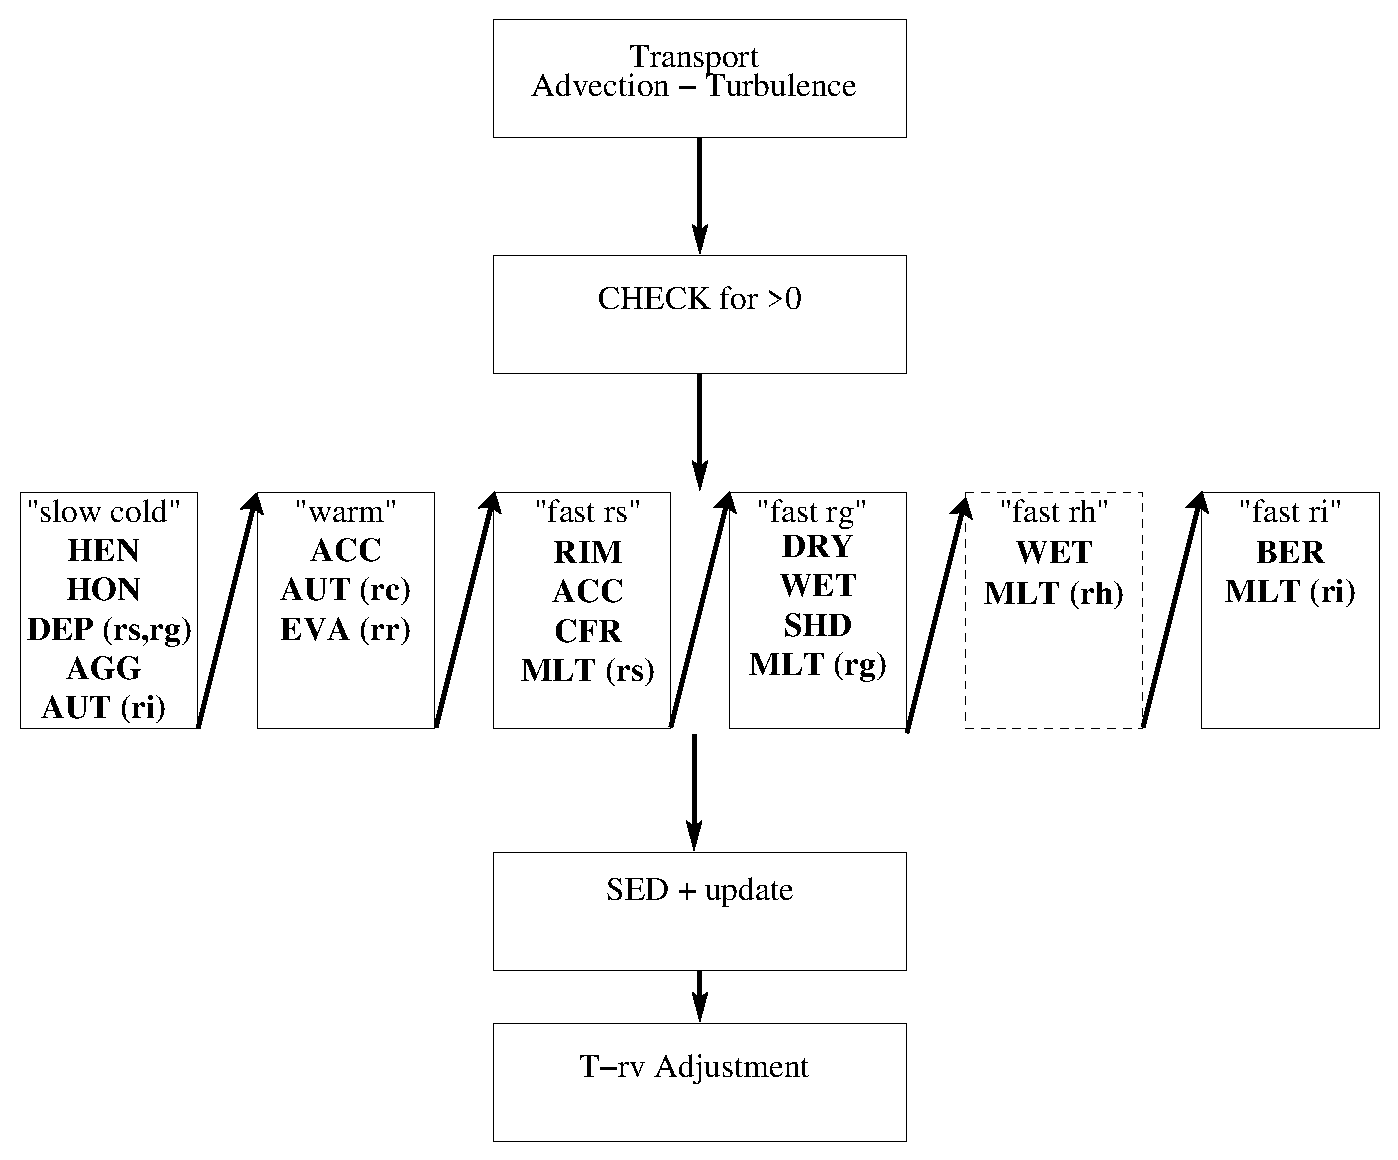
\includegraphics[width=\textwidth]{\EPSDIR/integ_flow.eps}}
\caption{Algorithm of the step-by-step integration of the microphysical processes.}
\label{mixfigalgo}
\end{figure}

%
\subsection{Water vapor adjustments}\label{VAPADJ}
%
All the concurrent microphysical processes involving an exchange of heat and
water vapor on the condensed particles are computed independently each other.
In the warm microphysical scheme an implicit adjustment of the temperature,
water vapor and cloud water fields is performed in order to introduce some
consistency between $\theta$ and $r_v$ with a strict saturation criterium in
clouds leading to a subsequent passive adjustment of $r_c$. A by-product of this
adjustment is the derivation of a condensation/evaporation rate ($RVCNDC$) of
the cloud droplets. In mixed phase clouds the problem is far more complex
because of the presence of cloud droplets and ice (so two species to re-adjust)
and the difficulty of defining unambiguously a single level of saturation. The
solution which has been chosen here is to perform an implicit adjustment as in
Lord et al. (1984) or in Tao et al. (1989) because it seems superior to the
explicit closure exposed in Ferrier (1994) where a simple saturation over ice
is assumed leading to some controversial account of the Bergeron-Findeisen
effect\footnotemark
%
\footnotetext{Note that Krueger et al. (1995) emphasized the fact that the
original adjustment introduced by Lord et al. (1984) cannot reproduce an
implicit Bergeron-Findeisen transfer of mass}
%
and a single correction of $r_i$. In the present scheme
the Bergeron-Findeisen conversion rate ($RCBERI$) is explicitly pre-integrated
and so the traditional linear partition of water vapor correction as a function
of temperature can be subjected to some revision. Another advantage of using an
implicit adjustment scheme in the spirit of that of Lord et al. (1984) is that
it can revert to a classical adjustment
scheme in case of warm cloud ($r_i=0$) or fully glaciated cloud ($r_c=0$).

The major assumptions used in the proposed saturation adjustment scheme are the
following:

\begin{itemize}
\item the saturation vapor mixing ratio ($r_{{vs}_{iw}}$) inside a mixed phase
cloud results from the barycentric formula introduced by Lord et al. (1984)
that is:
%
\be\label{SAT2}
r_{{vs}_{iw}}=\frac{\displaystyle{r_c^* r_{{vs}_{w}}(T)+r_i^* r_{{vs}_{i}}(T)}}
                   {\displaystyle{r_c^* + r_i^* }}
\ee
%
\item the super/sub-saturation adjustment over cloud ice/droplets is made
isobarically and proportionnal to the explicitly estimated cloud water and
cloud ice content, this gives:
%
\be\label{SAT3}
\Delta r_c= r_c-r_c^*=\Delta r_v CND \qquad {\rm and} \qquad
\Delta r_i= r_i-r_i^*=\Delta r_v DEP
\ee
%
\noindent with
%
\be\label{SAT4}
\Delta r_v= r_v^*-r_v=r_v^*-r_{{vs}_{iw}}
\ee
%
\noindent and with
%
\be\label{SAT5}
CND=\frac{\displaystyle{r_c^*}}{\displaystyle{r_c^*+r_i^*}} \qquad
{\rm and} \qquad
DEP=\frac{\displaystyle{r_i^*}}{\displaystyle{r_c^*+r_i^*}}.
\ee
%
So any deficit or excess of water vapor is compensated or absorbed by each
cloudy condensed phase in proportion to their respective content and as a
consequence, $\Delta r_c$ and $\Delta r_i$ have always the same sign. This way
of doing seems raisonnable since once the Bergeron-Findeisen effect is
accounted for, water vapor can be supplied or gathered by $r_c$ and $r_i$ in
proportion to their actual amount\footnotemark
%
\footnotetext{In the remaining text, the starred variables are the most recently
updated (or "guess") variables}
%
.

However, the above adjustment formulation was found to produce to much ice at weakly negative temperature. As a consequence, since the Masdev 4.1 version, the $CND$ and $DEP$ terms are calculated following Tao et al. (1989) as:
\be\label{SAT5NEW}
CND=\frac{T - T_{00} }{T_0 - T_{00} }\qquad
{\rm and} \qquad
DEP=1 - CND \qquad
\ee
with $T_0 = 0^\circ$C  and $T_{00} = 40^\circ$C.

\end{itemize}
The saturation adjustment then proceeds as for Tao et al. (1989) where a
zero-crossing solution of
%
\be\label{SAT6}
\begin{array}{rl}
F(T)&=T-T^*-\frac{\displaystyle{L_v(T) \Delta r_c + L_s(T) \Delta r_i}}
           {\displaystyle{C_{ph}}} \\
  &=T-T^*+\Big({\frac{\displaystyle{L_v(T) CND + L_s(T) DEP}}
                     {\displaystyle{C_{ph}}}}\Big)
                     (r_{{vs}_{iw}}(T)-r_v^*)
\end{array}
\ee
%
\noindent is sought using (\ref{SAT2}) to (\ref{SAT5}) and the non-iterative
algorithm of Langlois (1973) already experienced for the warm microphysical
adjustment is preferred to the first order solution of Tao et al. (1989). Of
course, this adjustment is performed after integrating explicitly all the source
terms in the $\theta$ and the $r_v$ prognostic equations, the cloud condensation
and ice deposition terms excepted.

The procedure used for solving (\ref{SAT6}) is based upon the quasi-second
order expansion of $F(T)=0$, namely\footnotemark
%
\footnotetext{The slow variations of $L_v(T)$ and of $L_s(T)$ with the
temperature are neglected but not those of $r_{{vs}_w}(T)$ and of
$r_{{vs}_i}(T)$.}
%
%
\begin{equation}\label{SAT7}
T \simeq T^*- \dfrac{F(T^*)}{F'(T^*)}
  \Big[ 1+ \dfrac{1}{2} \dfrac{F(T^*)}{F'(T^*)}  \dfrac{F''(T^*)}{F'(T^*)} \Big]
\end{equation}
%

\noindent where
%
\be\label{SAT8}
\begin{array}{rrl}
\Delta_1 &=
\dfrac{F(T^*)}{F'(T^*)}
&= \dfrac { \big [L_v(T^*) CND + L_s(T^*) DEP \big ]
   (r_c^* r_{{vs}_w}(T^*) +r_i^* r_{{vs}_i}(T^*) - (r_c^*+r_i^*) r_v^*) }
     {C_{ph}(r_c^*+r_i^*) + \big [L_v(T^*) CND +L_s(T^*) DEP\big ] \big [r_c^* r'_{{vs}_w}(T^*) + r_i^* r'_{{vs}_i}(T^*)\big ]}, \\
\Delta_2 &=
\dfrac{F''(T^*)}{F'(T^*)}
&= \dfrac { \big [L_v(T^*) CND + L_s(T^*) DEP \big ]
   (r_c^* r''_{{vs}_w}(T^*) +r_i^* r''_{{vs}_i}(T^*)) }
     {C_{ph}(r_c^*+r_i^*) + \big [L_v(T^*) CND +L_s(T^*) DEP\big ] \big [r_c^* r'_{{vs}_w}(T^*) + r_i^* r'_{{vs}_i}(T^*)\big ]}, \\
\end{array}
\ee
%
\noindent and where
%
\be\label{SAT9}
\begin{array}{rl}
r'_{{vs}_w}(T^*) &= A_w(T^*) r_{{vs}_w}(T^*) \Big[1 + \dfrac{r_{{vs}_w}(T^*)}{\epsilon} \Big], \\
r'_{{vs}_i}(T^*) &= A_i(T^*) r_{{vs}_i}(T^*) \Big[1 + \dfrac{r_{{vs}_i}(T^*)}{\epsilon} \Big], \\
r''_{{vs}_w}(T^*) &= r'_{{vs}_w}(T^*) \Big[ \dfrac{A'_w(T^*)}{A_w(T^*)}+A_w(T^*) \big(1+2\dfrac{r_{{vs}_w}(T^*)}{\epsilon}\big) \Big], \\
r''_{{vs}_i}(T^*) &= r'_{{vs}_i}(T^*) \Big[ \dfrac{A'_i(T^*)}{A_i(T^*)}+A_i(T^*) \big(1+2\dfrac{r_{{vs}_i}(T^*)}{\epsilon}\big) \Big]
\end{array}
\ee
%
\noindent with $\epsilon=M_v/M_d$ and
%
\be\label{SAT10}
\begin{array}{rcl}
A_w(T)=\dfrac{\beta_w}{T^2} - \dfrac{\gamma_w}{T}
&\qquad {\rm and} \qquad&
A'_w(T)=-\dfrac{2\beta_w}{T^3} + \dfrac{\gamma_w}{T^2} \\
A_i(T)=\dfrac{\beta_i}{T^2} - \dfrac{\gamma_i}{T}
&\qquad {\rm and} \qquad&
A'_i(T)=-\dfrac{2\beta_i}{T^3} + \dfrac{\gamma_i}{T^2}.
\end{array}
\ee
%

Finally the rates $RVDEPI$ and $RVCNDC$ in the $r_c$ and $r_i$ equations, are
estimated by:
%
\be\label{STA11}
\begin{array}{rrl}
RVDEPI &= \dfrac{(r_v^* - r_{{vs}_{iw}} )DEP}{2\Delta t}
&= \dfrac{C_{ph}}{L_v(T^*) CND + L_s(T^*) DEP} \Big[ -\Delta_1(1+\dfrac{1}{2} \Delta_1 \Delta_2) \Big]
\dfrac{DEP}{2\Delta t}\\
RVCNDC &= \dfrac{(r_v^* - r_{{vs}_{iw}} )CND}{2\Delta t}
&= \dfrac{C_{ph}}{L_v(T^*) CND + L_s(T^*) DEP} \Big[ -\Delta_1(1+\dfrac{1}{2} \Delta_1 \Delta_2) \Big]
\dfrac{CND}{2\Delta t}.
\end{array}
\ee
%


%\vfill
%
\section{References}
\label{section5}
%
\decrefname
B\"ohm, H. P., 1989:
      A general equation for the terminal fall speed of solid hydrometeors.
      {\it J. Atmos. Sci.},
      {\bf 46},
      2419-2427.
\decrefname
Caniaux, G., 1993:
      Param\'etrisation de la glace dans un mod\`ele non-hydrostatique de nuage:
      Application \`a une ligne de grain tropicale.
      {Th\`ese de Doctorat de l'Universit\'e Paul-Sabatier},
      257 pp.
\decrefname
Chaboureau, J.-P., J.-P. Cammas, P. J. Mascart, J.-P. Pinty, and J.-P. Lafore, 2002:
      Mesoscale model cloud scheme assessment using satellite observations.
      {\it J. Geophys. Res.}, {\bf 107(D16)}, 4301, doi:10.1029/2001JD000714.
\decrefname
Chaboureau, J.-P. and J.-P. Pinty, 2006:
      Evaluation of a cirrus parameterization with Meteosat Second Generation.
      {\it Geophys. Res. Let.}, {\bf 33}, L03815, doi:10.1029/2005GL024725.
\decrefname
Cheng, L., and M. English, 1983:
      A relationship between hailstone concentration and size.
      {\it J. Atmos. Sci.},
      {\bf 40},
      204-213.
\decrefname
Chin, H.-N. S., 1994:
      The impact of the ice phase and radiation on a midlatitude squall line
      system.
      {\it J. Atmos. Sci.},
      {\bf 51},
      3320-3343.
\decrefname
Cotton, W. R., G. J. Tripoli, R. M. Rauber and E. A. Mulvihill, 1986:
      Numerical simulations of the effects of varying ice crystal nucleation
      rates and aggregation processes on orographic snowfall.
      {\it J. Climate Appl. Meteor.},
      {\bf 25},
      1658-1680.
\decrefname
Farley, R. D., P. A. Price, H. D. Orville and J. H. Hirsch, 1989:
      On the numerical simulation of graupel/hail initiation via the riming of
      snow in bulk water microphysical cloud models.
      {\it J. Appl. Meteor.},
      {\bf 28},
      1128-1131.
\decrefname
Ferrier, B. S., 1994:
      A double-moment multiple phase four-class bulk ice scheme. Part I:
      description.
      {\it J. Atmos. Sci.},
      {\bf 51},
      249-280.
\decrefname
Ferrier, B. S., W.-K. Tao and J. Simpson, 1995:
      A double-moment multiple phase four-class bulk ice scheme. Part II:
      simulations of convective storms in different large-scale environments and
      comparison with other bulk parameterizations.
      {\it J. Atmos. Sci.},
      {\bf 52},
      1001-1033.
\decrefname
Foote, G. B., and P. S. Du Toit, 1969:
      Terminal velocity of raindrops aloft.
      {\it J. Appl. Meteor.},
      {\bf 8},
      249-253.
\decrefname
Hall, W. D., and H. R. Pruppacher, 1977:
      The survival of ice particles falling from cirrus clouds in subsaturated
      air.
      {\it J. Atmos. Sci.},
      {\bf 33},
      1995-2006.
\decrefname
Hallett, J., and S. C. Mossop, 1974:
      Production of secondary ice particles during the riming process.
      {\it Nature},
      {\bf 249},
      26-28.
\decrefname
Heymsfield, A. J., 1972:
      Ice crystals terminal velocities.
      {\it J. Atmos. Sci.},
      {\bf 29},
      1348-1356.
\decrefname
Heymsfield, A. J. and J. C. Pflaum, 1985:
      A quantitative assessment of the accuracy of techniques for calculating
      graupel growth.
      {\it J. Atmos. Sci.},
      {\bf 42},
      2264-2274.
\decrefname
Houze, R. A. Jr., P. V. Hobbs, P. H. Herzegh and D. B. Parsons, 1979:
      Size distributions of precipitation particles in frontal clouds.
      {\it J. Atmos. Sci.},
      {\bf 36},
      156-162.
\decrefname
Kajikawa, M., and A. J. Heymsfield, 1989:
      Aggregation of ice crystals in cirrus.
      description
      {\it J. Atmos. Sci.},
      {\bf 46},
      3108-3121.
\decrefname
Langlois, W. E., 1973:
      A rapidly convergent procedure for computing large-scale condensation in
      a dynamical weather model.
      {\it Tellus},
      {\bf 25},
      86-87.
\decrefname
Krueger, S. K., Q. Fu, K. N. Liou, and H.-N. S. Chin, 1995:
      Improvements of an ice-phase microphysics parameterization for use in
      numerical simulations of tropical convection.
      {\it J. Appl. Meteor.},
      {\bf 34},
      281-287.
\decrefname
Lascaux, F., E. Richard, and J.-P. Pinty, 2006:
      Numerical simulations of three MAP IOPs and the associated microphysical processes.
     {\it Quart. J. Roy. Meteor. Soc.}, {\bf 132}, 1907-1926.
\decrefname
Lin, Y.-L., R. D. Farley, and H. D. Orville, 1983:
      Bulk parameterization of snow field in a cloud model.
      {\it J. Climate Appl. Meteor.},
      {\bf 22},
      1065-1092.
\decrefname
Locatelli, J. D., and P. V. Hobbs, 1974:
      Fall speeds and masses of solid precipitation particles.
      {\it J. Geophys. Res.},
      {\bf 79D},
      2185-2197.
\decrefname
Lord, S. J., H. E. Willoughby, and J. M. Piotrowicz, 1984:
      Role of a parameterized ice-phase microphysics in an axisymmetric
      non-hydrostatic tropical  cyclone model.
      {\it J. Atmos. Sci.},
      {\bf 41},
      2836-2848.
\decrefname
Nelson, S. P., 1983:
      The influence of storm flow structureon hail growth.
      {\it J. Atmos. Sci.},
      {\bf 40},
      1965-1983.
\decrefname
Mc Cumber, M., W.-K. Tao, J. Simpson, R. Penc, and S. T. Soong, 1991:
      Comparaison of ice-phase microphysical parameterization schemes using
      numerical simulations of tropical convection.
      {\it J. Appl. Meteor.},
      {\bf 30},
      985-1004.
\decrefname
Mc Farquhar, G. M., A. J. Heymsfield, 1997:
      Parameterization of tropical cirrus ice crystal size distributions and
      implications for radiative transfer: Results from CEPEX
      {\it J. Atmos. Sci.},
      {\bf 54},
      2187-2200.
\decrefname
Masson, B. J., 1956:
      On the melting of hailstones.
      {\it Quart. J. R. Met. Soc.},
      {\bf 82},
      209-216.
\decrefname
Meyers, M. P., P. J. DeMott, and W. R. Cotton, 1992:
      New primary ice-nucleation parameterizations in an explicit cloud model.
      {\it J. Appl. Meteor.},
      {\bf 31},
      708-721.
\decrefname
Meyers, M. P., R. L. Walko, J. Y. Harrington and W. R. Cotton, 1996:
      New RAMS cloud microphysics parameterization. Part II: The two-moment
      scheme.
      {\it Atmos. Res.}
      {\bf 45},
      3-39.
\decrefname
Murakami, M., 1990:
      Numerical modeling of dynamical and microphysical evolution of an isolated
      convective cloud -the 19 July 1981 CCOPE cloud.
      {\it J. Meteor. Soc. Japan},
      {\bf 68},
      107-128.
\decrefname
Musil, D. J., 1970:
      Computer modeling of hailstone growth in feeder clouds.
      {\it J. Atmos. Sci.},
      {\bf 27},
      474-482.
\decrefname
Passarelli, R. E., Jr., 1978:
      An approximate analytical model of the vapor deposition and aggregation
      growth of snow.
      {\it J. Atmos. Sci.},
      {\bf 35},
      118-124.
\decrefname
Pruppacher, H. R., and J. D. Klett, 1978:
      {\it Microphysics of Clouds and Precipitation}.
      Reidel,714 pp.
\decrefname
Rutledge, S. A. and P. V. Hobbs, 1983:
      The mesoscale and microscale structure and organization of clouds and
      precipitation in midlatitude cyclones. Part VIII: A model for the
      "Seeder-Feeder" process in warm-frontal rainbands.
      {\it J. Atmos. Sci.},
      {\bf 40},
      1185-1206.
\decrefname
Rutledge, S. A. and P. V. Hobbs, 1984:
      The mesoscale and microscale structure and organization of clouds and
      precipitation in midlatitude cyclones. Part XII: A diagnostic modeling
      study of precipitation development in narrow cold-frontal rainbands.
      {\it J. Atmos. Sci.},
      {\bf 41},
      2949-2972.
\decrefname
Ryan, B. F., 2000: A bulk parameterization of the ice particle size
      distribution and the optical properties in ice clouds,
      {\it J. Atmos. Sci.}, {\bf 57}, 1436-1451.
\decrefname
Starr, D. O'C. and S. K. Cox, 1985:
      Cirrus clouds. Part I: A cirrus cloud model.
      {\it J. Atmos. Sci.},
      {\bf 42},
      2663-2681.
\decrefname
Sue Chen, and W. R. Cotton, 1988:
      The sensitivity of a simulated extratropical mesoscale convective system
      to longwave radiation and ice-phase microphysics.
      {\it J. Atmos. Sci.},
      {\bf 45},
      3897-3910.
\decrefname
Tao, W.-K., J. Simpson, and M. Mc Cumber, 1989:
      An ice-water saturation adjustment.
      {\it Mon. Wea. Rev.},
      {\bf 117},
      231-235.
\decrefname
Tripoli, G. J., P. J. Flatau, and W. R. Cotton, 1988:
      Generalized microphysics scheme for use in mesoscale cloud model.
      {\it Preprints 10$^{th}$ International Cloud Physics Conference}.
      Bad-Homburg. FRG August, 1988,
      109-111.
\decrefname
Walko, R. L., W. R. Cotton, M. P. Meyers, and J. Y. Harrington, 1995:
      New RAMS cloud microphysics parameterization. Part I: The single-moment
      scheme.
      {\it Atm. Res.},
      {\bf 38},
      29-62.
\decrefname
Yang M.-J. and R. A. Houze, 1995:
      Sensitivity of squall-line rear inflow to ice microphysics and
      environmental humidity.
      {\it Mon. Wea. Rev.},
      {\bf 123},
      3175-3193.
\decrefname
Ziegler, C. L., 1985:
      Retrieval of thermal and microphysical variables in observed convective
      storms. Part I: Model development and preliminary testing.
      {\it J. Atmos. Sci.},
      {\bf 42},
      1487-1509.
\decrefname
Ziegler, C. L., 1988:
      Retrieval of thermal and microphysical variables in observed convective
      storms. Part II: Sensitivity of cloud processes to variation of the
      microphysical parameterization.
      {\it J. Atmos. Sci.},
      {\bf 45},
      1072-1090.
\decrefname

%\end{document}

%%%%%%%%%%%%%%%%%%%%%%%%%%%%%%%%%%%%%%%%%%%%%%%%%%%%%%%%%%%%%%%%%%%%%%%%%%%%%%%
%%%%%%%%%%%%%%%%%%%%%%%%%%%%%%%%%%%%%%%%%%%%%%%%%%%%%%%%%%%%%%%%%%%%%%%%%%%%%%
%%%%%%%%%%%%%%%%%%%%%%%%%%%%%%%%%%%%%%%%%%%%%%%%%%%%%%%%%%%%%%%%%%%%%%%%%%%%%%
%%%%%%%%%%%%%%%%%%%%%%%%  END OF ICE MICROPHYSICS %%%%%%%%%%%%%%%%%%%%%%%%%%%
%%%%%%%%%%%%%%%%%%%%%%%%%%%%%%%%%%%%%%%%%%%%%%%%%%%%%%%%%%%%%%%%%%%%%%%%%%%%%%
%%%%%%%%%%%%%%%%%%%%%%%%%%%%%%%%%%%%%%%%%%%%%%%%%%%%%%%%%%%%%%%%%%%%%%%%%%%%%%



%%%%%%%%%%%%%%%%%%%%%%%%%%%%%%%%%%%%%%%%%%%%%%%%%%%%%%%%%%%%%%%%%%%%%%%%%%%%%%%
%%%%%%%%%%%%%%%%%%%%%%%%%%%%%%%%%%%%%%%%%%%%%%%%%%%%%%%%%%%%%%%%%%%%%%%%%%%%%%%
% CONTRIBUTION TO THE MESONH SCIENTIFIC DOCUMENTATION PART 3 (PHYSICS)
% Author: Benoit Vie
% Original: May 17, 2017
%%%%%%%%%%%%%%%%%%%%%%%%%%%%%%%%%%%%%%%%%%%%%%%%%%%%%%%%%%%%%%%%%%%%%%%%%%%%%%%
\chapter{The 2-moment mixed-phase microphysical scheme LIMA}
\minitoc


\section{General considerations}
This chapter describes the LIMA (Liquid Ice Multiple Aerosols) quasi two-moment microphysical scheme.
In short, LIMA relies on the prognostic evolution of an aerosol population, and the careful description of the nucleating properties that enable cloud droplets and pristine ice crystals to form from aerosols \citep{Vie2016}. 

\subsection{Thermodynamics basics}

\paragraph{Latent heat}
\begin{align}
 \label{latent-heat-vaporization}
 L_v(T) &= L_v(273.15) + (c_{pv} - c_{pw}) (T-273.15) \\
 \label{latent-heat-sublimation}
 L_s(T) &= L_s(273.15) + (c_{pv} - c_{pi}) (T-273.15)
\end{align}

\paragraph{Saturation vapor pressure}
~\\
Liquid water saturation:
\begin{equation}
 \label{saturation-pressure-water}
 e_{sw}(T) = \exp(\alpha_w - \frac{\beta_w}{T} - \gamma_w\mathrm{ln}(T))
\end{equation}
with
\begin{align}
 \alpha_w &= \mathrm{ln}(e_{sw}(273.15)) + \frac{\beta_w}{273.15} + \gamma_w\mathrm{ln}(273.15) \\
 \beta_w &= \frac{L_v(273.15)}{R_v} \gamma_w ~ 273.15 \\
 \gamma_w &= \frac{c_{pw} - c_{pv}}{R_v}
\end{align}

Ice saturation:
\begin{equation}
 \label{saturation-pressure-ice}
 e_{si}(T) = \exp(\alpha_i - \frac{\beta_i}{T} - \gamma_i\mathrm{ln}(T))
\end{equation}
with
\begin{align}
 \alpha_i &= \mathrm{ln}(e_{si}(273.15)) + \frac{\beta_i}{273.15} + \gamma_i\mathrm{ln}(273.15) \\
 \beta_i &= \frac{L_s(273.15)}{R_v} \gamma_i ~ 273.15 \\
 \gamma_i &= \frac{c_{pi} - c_{pv}}{R_v}
\end{align}

\paragraph{Saturation mixing ratio}
~\\
For a perfect gas, $PV=nRT$, so $m=PVM/RT$. The water vapor mass mixing ratio is the ratio of water vapor mass by dry air mass. Writing $e$ the water vapor partial pressure, and $P-e$ the dry air partial pressure, we have:
\begin{equation}
 r_v = \frac{m_v}{m_d} = \frac{e}{P-e} \frac{M_v}{M_d}
\end{equation}

So we can express the saturation water vapor mixing ratio with respect to liquid water:
\begin{equation}
 \label{saturation-mr-water}
 r_{sw}(T) = \frac{M_v e_{sw}(T)}{M_d (P - e_{sw}(T))}
\end{equation}

Similarly for ice saturation:
\begin{equation}
 \label{saturation-mr-ice}
 r_{si}(T) = \frac{M_v e_{si}(T)}{M_d (P - e_{si}(T))}
\end{equation}

\subsection{Representation of aerosols}

The number concentration $N$ is expressed in kg$^{-1}$. Aerosols are represented in LIMA by a superposition of an unlimited number of aerosol modes. Each mode and has its own activation properties, and can therefore be used as CCN to create cloud droplets, IFN to nucleate ice crystals, or as ``coated IFN''. This last type of aerosols acts as IFN coated with hydrophilic material. They have the ability to first form cloud droplets as standard CCN, and then have the ability to freeze these droplets by immersion nucleation when they are lifted to negative temperature regions.

All aerosol modes have a lognormal particle size distribution.

Each CCN mode has its own activation properties (currently to be chosen between two sets of parameters, for maritime or continental aerosols) and size distribution parameters (mean diameter and spectral width).

Four types of IFN are distinguished in the nucleation parameterization by \citet{Phillips2008} which was included in LIMA: small dust particles, large dust particles, black carbon, and organics. In LIMA, each IFN mode is composed of a given (fixed during the model initialization) fraction of each IFN type.

\paragraph{Free and activated areosols}
~\\
For CCN modes, two prognostic variables are used to track the aerosols, $N^{free}$ for the free aerosols and $N^{acti}$ for the aerosols in cloud droplets. We therefore retrieve the complete population by summing $N = N^{free} + N^{acti}$.

Similarly for IFN, we track both $N^{free}$ the number of free IFN and $N^{nucl}$ the number of IFN in ice crystals.

For ``coated IFN'', three prognostic variables are necessary: $N^{free}$ to track the number of free aerosols, $N^{acti}$ for the aerosols in cloud droplets and $N^{nucl}$ for the aerosols in ice crystals.

\paragraph{Size distribution}
~\\
Each aerosol mode $m$ follows a lognormal particle size distribution with $r_m=D_m/2$ and $\sigma_m$:
\begin{equation}
 n_m(D) \mathrm{d}D = N_m \frac{1}{\sqrt{2\pi}~D~ln(\sigma_m)}e^{-\left(\frac{ln(D/D_m)}{\sqrt{2}ln(\sigma_m)}\right)^2} \mathrm{d}D
\end{equation}
with $n_m(D)$ (resp. $N_m$) the number concentration (kg$^{-1}$~m$^{-1}$, resp. kg$^{-1}$) for aerosols with a diameter between $D$ et $D+\mathrm d D$ (resp. total number concentration).

\paragraph{Moments of the size distribution}
~\\
The $p$ order moment $M(p)$ of the size distribution is:
\begin{equation}
 M(p) = D_m^p \exp\left( \frac{p^2 ln(\sigma_m)^2}{2} \right)
\end{equation}


\subsection{Representation of hydrometeors}
\label{hydrometeors}

Hydrometeors are classified in 6 different species as in the ICE4 scheme: cloud droplets, rain drops, pristine ice crystals, snow/aggregates, graupel, and hail. A 2-moment representation was adopted in LIMA for cloud droplets, rain drops and pristine ice crystals. Thus, for these three hydrometeor species, two prognostic variables are used: the mass mixing ratio $r$ (kg~kg$^{-1}$) and the number concentration $N$ (kg$^{-1}$). For precipitating ice species (snow/aggregates, graupel, hail), the 1-moment representation from ICE4 was kept, and the only prognostic variable is the mass mixing ratio $r$.

\subsubsection{Size distribution}

The size distribution of all hydrometeors in LIMA follows a generalized gamma law:
\begin{equation}
 \label{gamma-gen}
 n(D) \mathrm d D= N \frac{\alpha}{\Gamma(\nu)} (\lambda D)^{\alpha\nu} D^{-1} e^{-(\lambda D)^{\alpha}} \mathrm d D
\end{equation}
with $n(D)$ (resp. $N$) the number concentration (kg$^{-1}$~m$^{-1}$, resp. kg$^{-1}$) for particles with a diameter between $D$ et $D+\mathrm d D$ (resp. total number concentration).

Values for parameters $\alpha$ et $\nu$ are usually (they can be chosen in the EXSEG1 namelist at runtime, e.g.\ XALPHAR et XNUR, those indicated in Table \ref{hydrometeors-parameters}. $\lambda$ depends on the local mass mixing ratio and number concentration.

When $\alpha = 1$ and $\nu = 1$, the size distribution becomes:
\begin{equation}
 n(D) \mathrm d D= N \lambda e^{-\lambda D} \mathrm d D
\end{equation}

\paragraph{Moments of the size distribution}
~\\
The $p$ order moment $M(p)$ of the size distribution is:
\begin{equation}
 M(p) = \frac{1}{\lambda^p} \frac{\Gamma(\nu+p/\alpha)}{\Gamma(\nu)}
\end{equation}

The mean diameter and variance are:
\begin{align}
 \bar{D} &= \frac{1}{\lambda} \frac{\Gamma(\nu+1/\alpha)}{\Gamma(\nu)} \\
 \sigma^2 &= \frac{1}{\lambda^2} \left( \frac{\Gamma(\nu+2/\alpha)}{\Gamma(\nu)} - \left(\frac{\Gamma(\nu+1/\alpha)}{\Gamma(\nu)}\right)^2 \right)
\end{align}

However, for cloud droplets and rain drops (assumed spherical), the mean volume diameter and its associated variance are more often used:
\begin{align}
 \bar{D} &= M(3)^{\frac{1}{3}} = \frac{1}{\lambda} \left(\frac{\Gamma(\nu+3/\alpha)}{\Gamma(\nu)}\right)^{\frac{1}{3}} \\
 \sigma^2 &= \frac{1}{\lambda^2} \left( \frac{\Gamma(\nu+6/\alpha)}{\Gamma(\nu)} - \left(\frac{\Gamma(\nu+3/\alpha)}{\Gamma(\nu)}\right)^2 \right)^{\frac{1}{3}}
\end{align}

\paragraph{Diagnostic number concentrations for snow/aggregates, graupel and hail}
~\\
A 1-moment representation of snow, graupel and hail was chosen in LIMA. The number concentrations are estimated using the parameterized relationship
\begin{equation}
 N = \frac{C \lambda^x}{\rho_d}
\end{equation}
where $C$ and $x$ are linked, as in the ICE3 scheme, by $\mathrm{log}_{10}(C) = -3.55 x + 3.89$ \citep{Caniaux1993}, and their values can be found in Table~\ref{hydrometeors-parameters}.

\paragraph{Relationships between $r$, $N$, $D_m$ and $\lambda$}
~\\
Combining the particle size distribution and the mass-diameter relationship, we get:
\begin{align}
 r &= \int_D m(D) n(D) \mathrm d D \\
 r &= a N \int_D D^b \frac{\alpha}{\Gamma(\nu)} (\lambda D)^{\alpha\nu} D^{-1} e^{-(\lambda D)^{\alpha}} \mathrm d D \\
 r &= a N M(b) \\
 r &= a N \frac{1}{\lambda^b} \frac{\Gamma(\nu+b/\alpha)}{\Gamma(\nu)}
\end{align}

Therefore, we can determine $\lambda$:
\begin{align}
 \lambda &= \left( a \frac{N}{r} \frac{\Gamma(\nu+b/\alpha)}{\Gamma(\nu)} \right)^{\frac{1}{b}} \quad \mathrm{for~2-moment~species} \\
 \lambda &= \left( a \frac{C}{\rho_d r} \frac{\Gamma(\nu+b/\alpha)}{\Gamma(\nu)} \right)^{\frac{1}{b-x}} \quad \mathrm{for~1-moment~species}
\end{align}

For spherical droplets and drops ($b=3$), we get the mean volume diameter $D_m$ and $\lambda$ as:
\begin{align}
 \bar{D} &= \left( \frac{r}{a N} \right)^{\frac{1}{3}} \\
 \lambda &= \left( a \frac{N}{r} \frac{\Gamma(\nu+3/\alpha)}{\Gamma(\nu)} \right)^{\frac{1}{3}}
\end{align}
where the equation for $\lambda$ can be simplified if $\alpha=1$ and $\nu=1$:
\begin{equation}
  \lambda = \left( a \frac{N}{r} \Gamma(4) \right)^{\frac{1}{3}}
\end{equation}

\paragraph{The $\Gamma$ function}
~\\
\begin{align}
 \Gamma(x) &= \int_0^\infty t^{x-1} e^{-t} \mathrm{d}t \\
 \Gamma(x+1) &= x\Gamma(x) \\
 \Gamma(n+1) &= n! \quad (n \in \mathbb{N}) \\
 \Gamma(1/2) &= \sqrt{\pi} \\
 \Gamma(1) &= 1
\end{align}

\subsubsection{Mass-diameter relationship}

For all hydrometeors, the mass-diameter relationship takes the form $m(D)=aD^b$. Values for $a$ et $b$ are found in Table \ref{hydrometeors-parameters}. For icy hydrometeors, they account for the shape and density of ice particles. For cloud droplets and rain drops (assumed spherical), they are equivalent to:
\begin{equation}
 \label{mD}
 m(D) = \frac{4}{3} \pi \left(\frac{D}{2}\right)^3 \rho_{w}
\end{equation}

\subsubsection{Terminal fall speed}

For all hydrometeors, the terminal fall speed also depends on the diameter through the following equation, where values for $c$ et $d$ are again found in Table \ref{hydrometeors-parameters}:
\begin{equation}
 v(D)=\left(\frac{\rho_{0}}{\rho_{d}}\right)^{0.4} cD^d
\end{equation}

The air density correction term comes from \citet{Foote1969} and is based on the air density $\rho_{0}$ = 1.2041 kg~m$^{-3}$ at P = 1013.25~hPa and T = 293.15~K.

Values for $c$ and $d$ come from:
\begin{itemize}
 \item \citet[][Eq.\ (10-138)]{Pruppacher1997} for cloud droplets, with P = 1013.25~hPa and T = 293.15~K.
 \item \citet[][Eq.\ (2.22)]{Liu1969} for rain drops. They fitted data from the Smithsonian Meteorological Tables \citep{List1958} valid at P = 1013.25~hPa and T = 293.15~K.
 \item \citet[][Table B.2, for sizes between 0 and 200 $\mu$m]{Starr1985}, who modified relationships from \citet{Heymsfield1972}, valid at 400~hPa. The value for $c$ is corrected to use $D$ in m, and multiplied by $(0.58/\rho_{0})^{0.4}$ (assuming that the air density at 400~hPa is 0.58~kg~m$^{-3}$) so that the previous equation can be used.
 \item \citet[][]{Locatelli1974} for snow (their parameters for aggregates of densely rimed radiating assemblages of dendrites) and graupel (their second set of values for lump graupel), converted for $D$ in m. They do not specify the air pressure or temperature. Considering their experimental set-up, we assume P = 900~hPa (altitudes between 750 and 1500~m) and T = 273.15~K, and therefore multiply $c$ by $(1.15/\rho_{0})^{0.4}$.
 \item \citet[][]{Bohm1989} for hail, valid at $\rho_d$ = 1.1 kg~m$^{-3}$. The value of $c$  was changed to use $D$ in m and adapt to the previous equation again.
\end{itemize}

\begin{table}
\caption{Set of parameters used to characterize each hydrometeor category}
\begin{center}\label{hydrometeors-parameters}
\begin{tabular}{|c||c|c|c|c|c|c|c|c|}
\hline 
            & $r_c$ & $r_r$ & \multicolumn{3}{|c|}{$r_i$} & $r_s$ & $r_g$ & $r_h$ \\
            &       &       & plates & columns & rosettes &       &       &       \\
\hline \hline
$\alpha$    & 3 & 1 & \multicolumn{3}{|c|}{3} & 1 & 1 & 1 \\
$\nu$       & 1 & 2 & \multicolumn{3}{|c|}{3} & 1 & 1 & 8 \\
\hline
$a$         & $\rho_w \pi / 6$ & $\rho_w \pi / 6$ & 0.82 & $2.14~10^{-3}$ & 44 & 0.02 & 19.6 & 470 \\
$b$         & 3 & 3 & 2.5 & 1.7 & 3 & 1.9 & 2.8 & 3 \\
\hline
$c$         & $2.98~10^7$ & 842 & 747 & $1.96~10^5$ & $4~10^5$ & 5 & 122 & 201 \\
$d$         & 2 & 0.8 & 1 & 1.585 & 1.663 & 0.27 & 0.66 & 0.64 \\
\hline
$C$         & - & - & \multicolumn{3}{|c|}{-} & 5 & $5~10^5$ & $4~10^4$ \\
$x$         & - & - & \multicolumn{3}{|c|}{-} & 1 & -0.5 & -1 \\
\hline
$\bar{f}_0$ & 1 & 0.78 & \multicolumn{3}{|c|}{1} & 0.86 & 0.86 & 0.86 \\
$\bar{f}_1$ & 0 & 0.308 & \multicolumn{3}{|c|}{0} & 0.28 & 0.28 & 0.28 \\
$\bar{f}_2$ & 0.108 & 0 & \multicolumn{3}{|c|}{0.14} & 0 & 0 & 0 \\
\hline
$C_1$       & 0.5 & 0.5 & $1/\pi$ & 0.8 & 0.5 & $1/\pi$ & 0.5 & 0.5 \\
\hline
\end{tabular}
\end{center}
\end{table}


\section{CCN activation to form cloud droplets}

CCN activation in LIMA follows the parameterization from the C2R2 scheme, and was extended to treat the competition between several CCN modes. It is based on the same method to determine first a diagnostic maximum supersaturation (which depends mostly on the aerosol population, the vertical lifting and the cooling rate). The number of activated CCN in each mode is then computed using the activation spectrum of each mode.

\subsection{Activation spectrum}

For each hydrophilic aerosol mode (considered chemically homogeneous), the activation spectrum is parameterized after \citet{Cohard1998} as a function of the supersaturation $S_w$  (with $S_w=0.01$ for a 1\% supersaturation):
\begin{equation}
\label{SpectreCPB98}
 N_m^{CCN} = C_m S_w^{k_m} F(\mu_m,\frac{k_m}{2},\frac{k_m}{2}+1,-\beta_m S_w^2)
\end{equation}
where $C_m$, $k_m$, $\mu_m$ and $\beta_m$ depend on the aerosol population, and $F$ is the hypergeometric function \citep{Gradshteyn1965}\footnote{Note that in \citet{Cohard1998} $S_\%=100 S_w$ is used instead of $S_w$. Values for $\beta_m$ and $C_m$ are therefore adapted in LIMA: $\beta_m = 100^2 \beta_m$ and $C_m = 100^{k_m} C_m$}. Some properties of this activation spectrum are presented in the appendices of \citet{Cohard2000spectre}, such as:
\begin{align}
  \label{limiteCCN}
 \lim_{S_w \to \infty} N_m^{CCN} &= \frac{C_m}{\beta_m^{k_m/2}}\frac{\Gamma(k_m/2+1)\Gamma(\mu_m-k_m/2)}{\Gamma(\mu_m)} ~~;~~ k_m<2\mu_m \\
 \frac{\partial N_m^{CCN}}{\partial S_w} &= k_m C_m S_w^{k_m-1} (1+\beta_m S_w^2)^{-\mu_m}
\end{align}

$k_m$, $\beta_m$ and $\mu_m$ parameters are determined following \citet{Cohard2000spectre}:
\begin{align}
 \frac{k_m}{k_0} &= \left(\frac{ln(\sigma_m)}{ln(\sigma_0)}\right)^{\alpha_k^\sigma} \\
% 
 \frac{\beta_m}{\beta_0} &= \left(\frac{r_m}{r_0}\right)^{\alpha_\beta^r}  exp\left\{\alpha_\beta^\sigma \left[\frac{ln(\sigma_m)}{ln(\sigma_0)}-1\right]\right\}  \left(\frac{\epsilon_m}{\epsilon_{0}}\right)^{\alpha_\beta^{\epsilon_m}}  \left(\frac{T_m}{T_0}\right)^{\alpha_\beta^T} \\
% 
 \frac{\mu_m}{\mu_0} &= \left(\frac{ln(\sigma_m)}{ln(\sigma_0)}\right)^{\alpha_\mu^\sigma}
\end{align}
where $r_m$ and $\sigma_m$ are the parameters defining the aerosol particle size distribution. Reference values $k_0$, $\beta_0$, $\mu_0$, $r_0$, $\sigma_0$, $T_0$ and $\epsilon_{m0}$ are given in Tables~1 and 2 from \citet{Cohard2000spectre} for marine and continental aerosols. \citet{Cohard2000spectre} also explain how to compute the $\alpha_\bullet^\bullet$ parameters.

$C_m$ can then be determined using Eq.\ (\ref{limiteCCN}) considering that all available aerosols are activated when the supersaturation tends to infinity.

\paragraph{Implementation in LIMA}
~\\
In \emph{init\_aerosol\_properties.f90}, parameters $k_m$, $\beta_m$ and $\mu_m$ are computed for each CCN mode, in the variables XKHEN\_MULTI, XMUHEN\_MULTI and XBETAHEN\_MULTI (when the HINI\_CCN variable is set to AER). Since the number concentration of aerosols is a prognostic variable, $C_m$ cannot be computed during the initialization. However, the variable XLIMIT\_FACTOR is computed and $C_m$ at each grid point and time step will simply be derived as $C_m=N_m/\mathrm{XLIMIT\_FACTOR}$.

\subsection{Diagnostic maximum supersaturation}

This parameterization is adapted from \citet{Cohard1998}. The evolution of $S$ is described by Eq.~(\ref{S_evol}), where the three terms represent the effects of (1) the vertical lifting, (2) the cloud droplets growth by vapor condensation, and (3) the cooling rate. This equation is derived from \citet[][their Eqs.\ (13)-(29)]{Pruppacher1997}, using the assumption $1+S_w \approx 1$, and is therefore valid only at, or close to, saturation.
\begin{equation}
  \label{S_evol}
  \frac{\textnormal{d} S}{\textnormal{d} t} = \underbrace{\psi_1 \omega}_{(1)} - \underbrace{\psi_2 \frac{\textnormal{d} q_c}{\textnormal{d} t}}_{(2)}+\underbrace{\psi_3 \frac{\textnormal{d} T}{\textnormal{d} t}}_{(3)}
\end{equation}
where $\psi_1$, $\psi_2$ and $\psi_3$ are thermodynamical functions depending on $T$ and $P$ \citep{Cohard1998}:
\begin{align}
 \psi_1(T,P) &= \frac{g}{TR_d} \left( \frac{M_vL_v}{M_dc_{pd}T}-1 \right) \\
 %
 \psi_2(T,P) &= \frac{M_dP}{M_v e_{sw}(T)} + \frac{M_v L_v^2}{M_d R_d T^2 c_{pd}} = \frac{M_dP}{M_v e_{sw}(T)} + \frac{L_v^2}{T^2 c_{pd} R_v} \\
 %
 \psi_3(T,P) &= - \frac{M_v L_v}{M_d R_d T^2}
\end{align}

The following resolving method is similar to the solution from \citet{Pruppacher1997} and \citet{Cohard1998}, who did not account for the cooling rate [Eq.~(\ref{S_evol}), term 3].

Following \citet[][their Eqs.\ (13)-(34)]{Pruppacher1997}, the cloud droplet growth at a supersaturation $S_w$ follows:
\begin{equation}
 \frac{\mathrm{d}m}{\mathrm{d}t} = 2 \pi \rho_w \left(\frac{2}{\rho_w}A_w^{-1}\right)^{3/2} S_w \left[ \int_{\tau}^t S_w(t')\mathrm{d}t' \right]^{1/2}
\end{equation}
where $\tau$ is the time at which the considered droplet was activated, and $A_w$ a thermodynamical function:
\begin{equation}
 A_w = \frac{R_vT}{D_v e_{sw}(T)} + \frac{L_v}{k_aT}\left(\frac{L_v}{R_vT}-1\right) \simeq \frac{R_vT}{D_v e_{sw}(T)} + \frac{L_v^2}{k_aR_vT^2}
\end{equation}

Writing $n_m^{CCN}(S_w)\mathrm{d}S_w$ the number of activated droplets for one CCN mode $m$, and for a supersaturation between $S_w$ and $S_w+\mathrm{d}S_w$, we have:
\begin{equation}
 \int_0^{S_w} n_m^{CCN}(S')\mathrm{d}S' = N_m^{CCN}(S_w) = C_m S_w^{k_m} F(\mu_m,\frac{k_m}{2},\frac{k_m}{2}+1,-\beta_m S_w^2)
\end{equation}
and then
\begin{equation}
 n_m^{CCN}(S_w) = k_m C_m S_w^{k_m-1} (1+\beta_m S_w^2)^{-\mu_m} 
\end{equation}

When several CCN modes are present, we get:
\begin{equation}
 n^{CCN}(S_w) = \sum_{m~modes} k_m C_m S_w^{k_m-1} (1+\beta_m S_w^2)^{-\mu_m}
\end{equation}

Integrating over all the cloud droplets, the cloud water mass mixing ratio change is:
\begin{equation}
 \frac{\mathrm{d}q_c}{\mathrm{d}t} = 2 \pi \frac{\rho_w}{\rho_d} \left(\frac{2}{\rho_w} A_w^{-1}\right)^{3/2} S_w ~~ \int_0^{S_w} n^{CCN}(S') \left[ \int_{\tau(S')}^t S_w(t')\mathrm{d}t' \right]^{1/2} \mathrm{d}S'
\end{equation}

This equation cannot be solved analytically, but the temporal integral of supersaturation admits a lower bound, which helps us determine an upper bound $S_{max}$ for the supersaturation. Twomey proposed \citep[their Eqs.\ (13)-(37)]{Pruppacher1997} the following lower bound:
\begin{equation}
 \int_{\tau(S')}^t S_w(t')\mathrm{d}t' > \frac{S_w^2-S'^2}{2(\psi_1 \omega)}
\end{equation}
which becomes, when accounting for the cooling rate:
\begin{equation}
 \int_{\tau(S')}^t S_w(t')\mathrm{d}t' > \frac{S_w^2-S'^2}{2(\psi_1 \omega + \psi_3 \mathrm{d}T/\mathrm{d}t)}
\end{equation}

Thus:
\begin{equation}
 \frac{\mathrm{d}r_c}{\mathrm{d}t} > \frac{2 \pi \rho_w \left(\frac{2}{\rho_w} A_w^{-1}\right)^{3/2} S_w}{\rho_d ~ [2(\psi_1 \omega + \psi_3 \mathrm{d}T/\mathrm{d}t)]^{1/2}} \sum_{m~modes} \bigg[ k_m C_m \underbrace{\int_0^{S_w}  S'^{k_m-1} (1+\beta_m S'^2)^{-\mu_m} (S_w^2-S'^2)^{1/2} \mathrm{d}S'}_{I} \bigg]
\end{equation}

Using the variable change $x=(S'/S)^2$, \citet{Cohard1998} get:
\begin{equation}
 I = \frac{S_w^{k_m+1}}{2} \underbrace{B\left(\frac{k_m}{2},\frac{3}{2}\right)}_{B_m} \underbrace{F\left(\mu_m,\frac{k_m}{2},\frac{k_m+3}{2},-\beta_mS_w^2\right)}_{F_{3/2,m,S_w}}
\end{equation}
and
\begin{equation}
  \label{borne_rc}
 \frac{\mathrm{d}r_c}{\mathrm{d}t} > \frac{2 \pi \rho_w \rho_w^{-3/2} A_w^{-3/2} }{\rho_d ~ (\psi_1 \omega + \psi_3 \mathrm{d}T/\mathrm{d}t)^{1/2}} \sum_{m~modes} \bigg[ C_m k_m S_w^{k_m+2} B_m F_{3/2,m,S_w} \bigg]
\end{equation}

For the maximum supersaturation, we have $\mathrm{d}S/\mathrm{d}t=0$. Using Eqs.\ (\ref{S_evol}) and (\ref{borne_rc}) gives:
\begin{equation}
 \label{eq-smax}
 \sum_{m~modes} \bigg[ C_m k_m S_w^{k_m+2} B_m F_{3/2,m,S_w} \bigg] < \frac{\rho_d ~ (\psi_1 \omega + \psi_3 \mathrm{d}T/\mathrm{d}t)^{3/2}}{2 \pi \rho_w \rho_w^{-3/2} A_w^{-3/2} \psi_2}
\end{equation}
The diagnostic maximum supersaturation $S_{max}$ is the supersaturation for which the equality is reached, all other factors being determined by the aerosol population and atmospheric conditions.


\paragraph{Implementation in LIMA}
~\\
As presented in the previous section, $k_m$, $\beta_m$ and $\mu_m$, as well as the XLIMIT\_FACTOR parameter necessary to compute $C_m$, are initialized for each CCN mode in \emph{init\_aerosol\_properties.f90}. 

~\newline

In ini\_lima\_warm.f90:
\begin{itemize}
 \item For each aerosol mode, the function $F\left(\mu_m,\frac{k_m}{2},\frac{k_m+3}{2},-\beta_mS_w^2\right)$ of supersaturation $S_w$, used in Eq.\ (\ref{eq-smax}), is tabulated between two values ZSMIN et ZSMAX, with a logarithmic scale in $S_w$, in the XHYPF32 variable.
 \item For each aerosol mode, the function $F\left(\mu_m,\frac{k_m}{2},\frac{k_m}{2}+1,-\beta_mS_w^2\right)$ of supersaturation $S_w$, used in Eq.\ (\ref{SpectreCPB98}), is tabulated between the same two values ZSMIN et ZSMAX, with the same logarithmic scale in $S_w$, in the XHYPF12 variable.
 \item Functions $\psi_1$ and $\psi_3$ of $T$ are also tabulated, for $T$ from -40\textdegree C to +40\textdegree C, in the XPSI1 and XPSI3 variables.
 \item Eventually, the XAHENG$=(2 \pi \rho_w \rho_w^{-3/2} A_w^{-3/2} )^{-1}$ function is also tabulated on the same temperature domain.
\end{itemize}

~\newline

Eq.\ (\ref{eq-smax}) is solved in \emph{lima\_warm\_nucl.f90}:
\begin{itemize}
 \item $C_m$ for each CCN mode with $C_m = N_m/XLIMIT\_FACTOR$ (PTSTEP and ZRHODREF account for the unit change from $N_m$ to get $C_m$ in m$^{-3}$). $C_m$ is computed from the total aerosol population $N^{free}_m+N^{acti}_m$.
 \item $\psi_2$ is computed in ZZW1.
 \item Using a linear interpolation from the tabulated functions XPSI1, XPSI3 and XAHENG, we get ZZW3$= \frac{\rho_d}{\rho_w} \frac{(\psi_1 \omega + \psi_3 \mathrm{d}T/\mathrm{d}t)^{3/2}}{2 \pi \rho_w \rho_w^{-3/2} A_w^{-3/2} \psi_2}$
 \item Functions FUNCSMAX and SINGL\_FUNCSMAX compute the difference of the two terms in Eq.\ (\ref{eq-smax}).
 \item The maximum supersaturation $S_{max}$ is then determined by looking for a zero of this function for a supersaturation between ZS1 and ZS2 (ZS1 and ZS2 are chosen within the ZSMIN to ZSMAX range used to tabulate XHYPF32$=F_{3/2,m,S_w}$) using the Ridder algorithm \citep{Press1992}. 
\end{itemize}

\subsection{Number of activated cloud droplets}

According to the K\"{o}hler theory, for a given maximum supersaturation $S_{max}$, aerosols activated are exactly those with a critical supersaturation lower than $S_{max}$. Thus, to determine the number of aerosols really activated at time $t$, we first compute the number of activable aerosols for $S_{max}$ and the total aerosol population $N^{free}_m+N^{acti}_m$, using Eq.\ (\ref{SpectreCPB98}). The number of aerosols really activated is then the difference between the number of activable aerosols and the number of aerosols previously activated during the simulation $N^{acti}_m$:
\begin{align}
  \Delta N_m^{acti}(t) &= Max(0,N_m^{CCN}(S_{max})-N^{acti}_m(t-\Delta t)) \\
  N^{free}_m(t) &= N^{free}(t-\Delta t)-\Delta N_m^{acti}(t) \\ 
  N^{acti}_m(t) &= N^{acti}(t-\Delta t)+\Delta N_m^{acti}(t) 
\end{align}

\paragraph{Implementation in LIMA}
~\\
Computations are also led in \emph{lima\_warm\_nucl.f90}. ZTMP is the number of activable aerosols for each mode (using the tabulated function XHYPF12). The $N^{free}_m$ and $N^{acti}_m$ number concenterations for each mode are the updated.

A final test restrains the activation to regions where the total number of activable cloud droplets is higher than 25~cm$^{-3}$.




\section{Pristine ice nucleation}

Three ways to initiate pristine ice are parameterized in LIMA. The homogeneous nucleation of rain drops, cloud droplets and CCN is active only at very cold temperatures, below -35\textdegree C. Two parameterizations of the heterogeneous nucleation are available. The first one is based upon \citet{Meyers1992} and depends only on the atmospheric conditions. The second follows the empirical parameterization by \citet{Phillips2008}, and explicitly predicts the number of ice crystals formed from the nucleation of a prognostic IFN population.

The third way to create ice crystals in LIMA is the secondary production of ice by the Hallet-Mossop process when aggregates or graupel freeze cloud droplets. It is presented in the mixed phase collection processes presentation.

\subsection{Homogeneous ice nucleation}

Computations are carried in lima\_cold\_hom\_nucl.f90.

\subsubsection{Rain drops homogeneous freezing}

All raindrops are instantly transformed into graupel when they reach temperatures below -35\textdegree C.

\subsubsection{Cloud droplets homogeneous freezing}

The cloud droplet homogeneous freezing rate $J$ (number of ice embryos formed per cubic cm of water per second, cm$^{-3}$~s$^{-1}$) is taken from \citet{Eadie1971}, and was since used in many studies \citep[e.g.][]{Heymsfield1993,DeMott1994,Milbrandt2005b}:
\begin{align}
 \ln_{10}(J) &= \alpha_1 + \alpha_2 T + \alpha_3 T^2 +  \alpha_4 T^3 + \alpha_5 T^4 \\
 J &= \mathrm{exp} \Big[ \alpha_1 \mathrm{ln}(10) + \alpha_2 \mathrm{ln}(10)~T + \alpha_3 \mathrm{ln}(10)~T^2 +  \alpha_4 \mathrm{ln}(10)~T^3 + \alpha_5 \mathrm{ln}(10)~T^4 \Big]
\end{align}
with
\begin{align}
 \alpha_1 &= -606.3952 \\
 \alpha_2 &= -52.6611 \\
 \alpha_3 &= -1.7439 \\
 \alpha_4 &= -0.0265 \\
 \alpha_5 &= -1.536~10^{-4}\\
\end{align}

The probability for a raindrop of volume $V$ not to freeze in a time $\Delta t$ is given by:
\begin{equation}
 P = \mathrm{exp} [ -J~V~\Delta t ]
\end{equation}

\paragraph{Computations if $\alpha_c = 3$}
~\\
In this case the number of droplets that are not frozen can be derived:
\begin{align}
 N_c(t+\Delta t) &= \int_0^\infty \mathrm{exp}[ -J~\frac{\pi}{6}D^3~\Delta t ] n(D)dD \\
 &= \int_0^\infty e^{-J~\frac{\pi}{6}D^{\alpha_c}~\Delta t} N_c \frac{\alpha_c}{\Gamma(\nu_c)} \lambda_c^{\alpha_c \nu_c} D^{\alpha_c \nu_c - 1} e^{-(\lambda_c D)^{\alpha_c}} dD \quad \textrm{using~} \alpha_c = 3 \\
 &= \int_0^\infty N_c \frac{\alpha_c}{\Gamma(\nu_c)} \lambda_c^{\alpha_c \nu_c} D^{\alpha_c \nu_c - 1} e^{-D^{\alpha_c}(\lambda_c^{\alpha_c} + J \Delta t \pi / 6)} dD \\
 &= \int_0^\infty X^{-\alpha_c \nu_c} \lambda_c^{\alpha_c \nu_c} ~ ~ ~ N_c \frac{\alpha_c}{\Gamma(\nu_c)} X^{\alpha_c \nu_c} D^{\alpha_c \nu_c - 1} e^{-D^{\alpha_c} X^{\alpha_c}} dD \quad \textrm{with~} X = \left( \lambda_c^{\alpha_c} + \frac{J \Delta t \pi}{6} \right)^{1/\alpha_c} \\
 &= X^{-\alpha_c \nu_c} \lambda_c^{\alpha_c \nu_c} N_c \\
 &= \left( \frac{\lambda_c^{\alpha_c}}{\lambda_c^{\alpha_c} + \frac{J \Delta t \pi}{6}} \right)^{\nu_c} N_c\\
 &= \left( \frac{1}{1+\frac{1}{\lambda_c}\frac{J \Delta t \pi}{6}} \right)^{\nu_c} N_c
\end{align}
Similarly, for the mass of droplets that are not frozen, we get:
\begin{align}
 r_c(t+\Delta t) &= \left( \frac{1}{1+\frac{1}{\lambda_c}\frac{J \Delta t \pi}{6}} \right)^{\nu_c} N_c a \frac{1}{\lambda_c^3} \frac{\Gamma(\nu_c+3/\alpha_c)}{\Gamma(\nu_c)} \\
 &= \left( \frac{1}{1+\frac{1}{\lambda_c}\frac{J \Delta t \pi}{6}} \right)^{\nu_c} r_c
\end{align}

\paragraph{Computation if $\alpha_c \neq 3$}
~\\
In this case, an approximation is necessary, either by carrying the computations for the mean-volume diameter only, such as in \citet{Milbrandt2005b}, or by taking $1-\mathrm{exp}(-J V_c \Delta t) \approx J V_c \Delta t$ as in the ICE3 scheme. This case is not coded yet.

\subsubsection{CCN homogeneous freezing}

The homogeneous freezing of CCN particles follows \citet{Karcher2002}. Equations\ (12)-(28) from \citet{Pruppacher1997} become, with our notations, using the supersaturation $S_i = r_v / r_{si}$ \footnote{\citet{Pruppacher1997} use $s_{v,w}=r_v / r_{si} -1$.} and without the approximation $p-e = p$:
\begin{equation}
 \frac{\mathrm{d}S_i}{\mathrm{d}t} = \frac{p}{\epsilon e_{sat,i}} \frac{\mathrm{d}r_v}{\mathrm{d}t} - S_i \left( \frac{L_s \epsilon}{R_d T^2} \frac{\mathrm{d}T}{\mathrm{d}t} + \frac{g}{R_d T} w \right) 
\end{equation}
Using Eq.\ (12-26) and (12-29) from \citet{Pruppacher1997} with $\mu=0$ (entrainment effects are neglected):
\begin{equation}
 \frac{\mathrm{d}S_i}{\mathrm{d}t} = \left( \frac{L_s \epsilon g}{R_d T^2 c_{pd}} - \frac{g}{R_d T} \right) S_i w - \left( \frac{p}{\epsilon e_{sat,i}} + \frac{\epsilon L_s^2}{R_d T^2 c_{pd}} S_i\right) \frac{\mathrm{d}r_i}{\mathrm{d}t}
\end{equation}
Replacing $\epsilon = M_v / M_d$ and using the $M_d$, $M_v$, $R$, $R_d$, $R_v$ relationships, this equation takes the same form as Eq.\ (1) from \citet{Karcher2002}. They use $R_i$ (the number of water molecules deposited at the surface of ice crystals per unit of time and air volume, m$^{-3}$~s$^{-1}$), where we use the ice mass mixing ratio $r_i$ instead ($\mathrm{d}r_i/\mathrm{d}t = R_i m_w / \rho_d$), and therefore multiply $a_2$ and $a_3$ by $\rho_d / m_w$:
\begin{align}
 \frac{\mathrm{d}S_i}{\mathrm{d}t} &=  a_1 S_i w - (a_2 + a_3 S_i) \frac{\mathrm{d}r_i}{\mathrm{d}t} \\
 a_1 &= \frac{M_v L_s g}{R c_{pd} T^2} - \frac{M_d g}{R T} \\
 a_2 &= \frac{p}{\epsilon e_{sat,i}} \approx r_{si}^{-1}\\
 a_3 &= \frac{L_s^2}{R_v c_{pd} T^2}
\end{align}
Homogeneous freezing occurs when the supersaturation exceeds a critical value, depending on temperature, which they fitted with the following equation:
\begin{equation}
 S_{cr} = 2.583 - \frac{T}{207.83}
\end{equation}
The characteristic time of homogeneous nucleation is:
\begin{equation}
 \tau = c(T) \left( \left|\frac{\partial \ln(J)}{\partial T}\right| \right)_{S_i=S_{cr}} \frac{\mathrm{d}T}{\mathrm{d}t}
\end{equation}
where \citet{Karcher2002} obtained the following fits:
\begin{align}
 c(T) &= \mathrm{max}[100,100(22.6*0.1T)] \\
 \left. \frac{\partial \ln(J)}{\partial T}\right|_{S_i=S_{cr}} &= 4.37-0.03T
\end{align}

To compute the solution of homogeneous freezing, we need to evaluate the ratio $b_2 /2 \pi b_1$ where $b_1$ and $b_2$ are defined in their Eq.\ (7), for the peak supersaturation supposed to be $S_i^{max}=S_{cr}$. Using $m_w n_{sat} / \rho_d = r_{v,sat}$ ($n_{sat}$ is in m$^{-3}$) and $D_v(T,P) = 0.211 (T/T_0)^{1.94} (P_0/P)$ \citep[Eq.\ (13-3) from][with $D_v$ expressed in cm$^2$~s$^{-1}$]{Pruppacher1997}:
\begin{equation}
 \frac{b_2}{2 \pi b_1} = \frac{\rho_i}{\rho_d ~ 2 \pi~0.211~10^{-4} ~ (P_0/P) (T/T_0)^{1.94} ~ r_{si} (S_{cr}-1)}
\end{equation}

We use Eq.\ (11a) from \citet{Karcher2002} to compute the number of frozen CCN ($N_i$, kg$^{-1}$), dividing their right side by $\rho_d$ because their $n_i$ is expressed in m$^{-3}$, and multiplying by $\rho_d / m_w$ to convert our $a_2$ and $a_3$ parameters:
\begin{align}
 N_i &= \frac{1}{\rho_d} \frac{m_w}{\rho_i} \left( \frac{b_2}{2 \pi b_1} \right)^{3/2} \frac{a_1}{(a_2 + a_3 ~ S_{cr})(m_w/\rho_d)} \frac{w}{\sqrt{\tau}} \\
 &= \frac{1}{\rho_i} \left( \frac{b_2}{2 \pi b_1} \right)^{3/2} \frac{a_1}{a_2 + a_3 ~ S_{cr}} \frac{w}{\sqrt{\tau}}
\end{align}

Eventually, we determine the ice mass mixing ratio formed following their Eq.\ (11c), with the same transformations as for the previous one:
\begin{align}
 r_i &= \frac{1}{\rho_d} \frac{\pi}{6} m_w \frac{a_1}{(a_2 + a_3 ~ S_{cr})(m_w/\rho_d)} w \tau \\
 &= \frac{\pi}{6} \frac{a_1}{a_2 + a_3 ~ S_{cr}} w \tau \\
 &= \frac{\pi}{6} N_i~\rho_i \left(\frac{b_2}{2 \pi b_1}\right)^{-3/2} \tau^{3/2} 
\end{align}

\paragraph{Remarks on this parameterization}
~\\
\begin{itemize}
 \item As stated by \citet{Karcher2002}, this parameterization does not explicitely depend on the number of available aerosols, and the resulting number of ice particles formed is simply limited to the maximum number of available CCN.
 \item We assume in LIMA that only the fast growth case occurs (see their paragraph 27, p~5).
 \item They stated (paragraph 28, p~5) that $T_{cr}$ (the temperature at which the critical supersaturation $S_{cr}$ is reached) should be used in the computations. In LIMA, computations are currently carried with $T$.
\end{itemize}

\paragraph{Implementation in LIMA}
~\\
The following computations are carried once:
\begin{align}
 \mathrm{ZZY} &= S_{cr} \\
 \mathrm{ZPSI1} &= a_1 ~ S_{cr} \\
 \mathrm{ZPSI2} &= a_2 + a_3 ~ S_{cr} \\
 \mathrm{ZTAU} &= \tau \quad \quad \mathrm{(using~} \mathrm{d}T/\mathrm{d}t = \mathrm{ZTHS}~\left(P/P_{00}\right)^{R_d/c_{pd}} \mathrm{)} \\
 \mathrm{ZBFACT} &= \frac{b_2}{2 \pi b_1} \quad \mathrm{(using~} S_i/r_v = r_{v,sat}^{-1} \mathrm{)} \\
 \mathrm{ZZX} &= \frac{1}{\Delta t} N_i \quad \mathrm{limited~between~0~and~ZNFS} \\
 \mathrm{ZZW} &= \frac{1}{\Delta t} r_i \quad \mathrm{limited~to~ZRVS}
\end{align}

CCN homogeneous freezing is supposed to act equally on each CCN mode, and the number of frozen CCN is depleted from each mode in proportion of the initial number of available CCN in each mode.

\subsection{Heterogeneous pristine ice nucleation following \citet{Meyers1992}}

The ice nucleation parameterization by \citet{Meyers1992} links the number concentration of ice crystals to the supersaturation only.

\subsubsection{Heterogeneous nucleation by deposition}

Using data from continuous flow chambers, \citet[][Eq.\ (2.4)]{Meyers1992} expressed the number of ice forming nuclei as a function of the supersaturation with respect to ice (using the decimal form of $S_{i}$, so that $S_i=0.01$ for a 1\% supersaturation):
\begin{equation}
 N_{IN}(S_{i}) [L^{-1}] = \exp[12.96~10^{-2}~100~S_{i} - 0.639]
\end{equation}

This parameterization is easily implemented in LIMA.

First, some variables are initialized in \emph{ini\_lima\_cold\_mixed.f90}:
\begin{itemize}
 \item $\mathrm{XNUC\_DEP} = 1000 ~ \mathrm{XFACTNUC\_DEP} ~ \mathrm{ZFACT\_NUCL}$, where the $1000$ factor is used to convert from the previous formula to concentrations in m$^{-3}$, XFACTNUC\_DEP (default value 1) can be changed in namelist to modulate the ice nucleation process, and $ZFACT\_NUCL = 1$.
\end{itemize}

Then, in \emph{lima\_meyers.f90}, ZZY is computed where $T<5$\textdegree C and $S_i > 0$. The decimal formulation of $S_i$ is used in LIMA ($S_i = 0.01$ for a 1\% supersaturation), and the number concentrations are in kg$^{-1}$, so the pristine ice number concentration tendency is:
\begin{equation}
 \mathrm{ZZY [kg^{-1}s^{-1}]}= \frac{\mathrm{XNUC\_DEP}}{\rho_d \Delta t} \exp[12.96~10^{-2} ~ 100 ~ S_i - 0.639]
\end{equation}

To compute the mass mixing ratio created by this process, we first need to determine the number of ice crystals actually nucleated at this time step by subtracting the number of already nucleated ice crystals. The mass mixing ratio tendency is then deduced assuming that an ice embryo has a mass of $\mathrm{XMNU0} = 6.88$~10$^{-13}$~kg.

\subsubsection{Heterogeneous nucleation by contact}

\citet[][Eq.\ (2.6)]{Meyers1992} also expressed the number of ice crystals nucleated by contact freezing of cloud droplets as a function of temperature:
\begin{equation}
 N_{IN}(T) \mathrm{[L^{-1}]} = \exp[-2.80 - 0.262 (T-T_0)]
\end{equation}

This number is computed in the same way as the nucleation by deposition in LIMA, and the number concentration of crystals is limited by the number of available cloud droplets.

To compute the mass mixing ratio created by this process, we first need to determine the number of ice crystals actually nucleated at this time step by subtracting the number of already nucleated ice crystals. The mass mixing ratio tendency is then deduced assuming that the cloud droplets mass is evenly distributed among cloud droplets, so:
\begin{equation}
 ZZW = r_{i,contact} = \frac{r_c}{N_c} N_{i,contact}
\end{equation}

\subsection{IFN nucleation following the parameterization by \citet{Phillips2008}}

Instead of the parameterization by \citet{Meyers1992}, which does not link the pristine ice number concentration to the available aerosols, the parameterization proposed by \citet{Phillips2008,Phillips2013} can be used in LIMA. This implementation is described in \citet{Berthet2010these,Vie2016}.

\subsubsection{Reference activity spectrum}

Based on observations of ice nucleation in the continuous flow diffusion chamber (CFDC), \citet{Phillips2008} proposed a parameterization of the ice nucleation reference activity spectrum, taking the same form as the one proposed by \citet{Meyers1992}, but distinguishing three temperature regimes. Note that, as specified by \citet{Phillips2008}, $S_i$ is artificially prevented from exceeding water saturation in the computation of $N_{i,ref}$. For temperatures colder than -35\textdegree C, they got [their Eq.\ (2)]:
\begin{equation}
 N_{i,ref} (T,S_i) = \frac{1000}{\rho_{CFDC}} ~ \gamma ~ (\exp[12.96 (S_i-0.1)])^{0.3}
\end{equation}
For temperatures warmer than -25\textdegree C, they got ([Their Eq.\ (3)]:
\begin{equation}
 N_{i,ref} (T,S_i) = 0.058707 ~ \frac{1000}{\rho_{CFDC}} ~ \gamma ~ \exp[12.96 ~ S_i - 0.639]
\end{equation}
The reference activity spectrum for temperatures between -25\textdegree C and -35\textdegree C is a bit more complicated and involves intermediate computations [their Eqs.\ (4)-(7) and appendix A]:
\begin{align}
 N_{max}(T,S_i) &= \frac{1000}{\rho_{CFDC}} ~ \gamma ~ (\exp[12.96 (S_i^w-0.1)])^{0.3} \quad \quad \quad \quad \text{for T between -30\textdegree C and -35\textdegree C} \\
 N_{max}(T,S_i) &= 0.058707 ~ \frac{1000}{\rho_{CFDC}} ~ \gamma ~ \exp[12.96 ~ S_i^w - 0.639] \quad \text{ for T between -25\textdegree C and -30\textdegree C} \\
 \hat{n}(T,S_i) &= \min\bigg( 0.058707 ~ \frac{1000}{\rho_{CFDC}} ~ \gamma ~ \exp[12.96 ~ S_i - 0.639] ~ ~ ; ~ ~ n_{max}(T,S_i) \bigg) \\
 \tilde{n}(T,S_i) &= \min\bigg( \frac{1000}{\rho_{CFDC}} ~ \gamma ~ (\exp[12.96 (S_i-0.1)])^{0.3} ~ ~ ; ~ ~ n_{max}(T,S_i) \bigg) \\
 \bar{n}(T,S_i) &= \hat{n}(T,S_i) \left( \frac{\tilde{n}(T,S_i)}{\hat{n}(T,S_i)} \right)^{\delta_1^0(T,-35,-25)} \\
 N_{i,ref} (T,S_i) &= \min\Big( \bar{n}(T,S_i) ~ ; ~ N_{max}(T,S_i) \Big)
\end{align}

\subsubsection{Integration of the number of activable IFN}

The reference activity spectrum is used to predict the fraction of each IFN species $X$ which can be nucleated into ice crystals for given thermodynamical conditions, as \citep[Eq.\ (9) from][]{Phillips2008}:
\begin{equation}
 N_X^{IFN} = \int_{0.1~10^{-6}}^\infty \big[ 1 - \exp(- \mu_X(D,S_i,T)) \big] \frac{\mathrm{d}N_X}{\mathrm{d}D} \mathrm{d}D
\end{equation}
where the integration starts at 0.1~$\mu$m because we assume that smaller aerosols cannot form ice crystals.

The expression for $\mu_X$, and the parameters necessary to compute it, are found in \citet[][Eqs.\ (10)-(12) and Table 1]{Phillips2008}. Writing
\begin{equation}
 A(S_i,T) = H_X(S_i,T) \xi(T) \frac{\alpha_X N_{i,ref} (T,S_i)}{\Omega_{X,1,*}}
\end{equation}
we have
\begin{align}
 \mu_X(D,S_i,T) &= A(S_i,T) \frac{\mathrm{d}\Omega_X}{\mathrm{d}N_X} \\
 &\approx A(S_i,T) \pi D^2
\end{align}

Two methods are used to perform the integration, depending on the temperature.

\paragraph{For temperatures warmer than -35\textdegree C}
~\\
For temperatures warmer than -35\textdegree C, we assume that the number of ice crystals formed remains small, therefore $\mu_x << 1$ and we can write:
\begin{align}
 N_X^{IFN} &\approx \int_{0.1~10^{-6}}^\infty \mu_X(D,S_i,T) \frac{\mathrm{d}N_X}{\mathrm{d}D} \mathrm{d}D \\
 &\approx \int_{0.1~10^{-6}}^\infty \mu_X(D,S_i,T) n_X(D) \mathrm{d}D \\
 &\approx A(S_i,T) \pi N_X \int_{0.1~10^{-6}}^{\infty} D^2 n_X(D) \mathrm{d}D
\end{align}
We need to compute the integral in the previous equation:
\begin{align}
 \int_{0.1~10^{-6}}^{\infty} D^2 n_X(D) \mathrm{d}D &= \int_{0.1~10^{-6}}^{\infty} \frac{D^2}{\sqrt{2\pi} ~ D ~ \ln(\sigma_X)} e^{-\left( \frac{\ln(D/D_X)}{\sqrt2 \ln(\sigma_X)} \right)^2 } \mathrm{d}D
\end{align}
We proceed to the variable change:
\begin{align*}
 x &= \frac{\ln(D/D_X)}{\sqrt2 \ln(\sigma_X)} \\
 D &= D_X e^{x \sqrt2 \ln(\sigma_X)} \\
 \mathrm{d}D &= \sqrt2 \ln(\sigma_X) D_X e^{x \sqrt2 \ln(\sigma_X)} \mathrm{d}x
\end{align*}
which gives:
\begin{align}
 \int_{0.1~10^{-6}}^{\infty} D^2 n_X(D) \mathrm{d}D &= \int_{B}^{\infty} \frac{D_X^2}{\sqrt{\pi}} e^{2 \sqrt2 x \ln(\sigma_X) - x^2} \mathrm{d}x \quad \mathrm{with} \quad B = \frac{\ln(0.1~10^{-6} / D_X)}{\sqrt{2} \ln(\sigma_X)} \\
 &= \frac{D_X^2}{\sqrt{\pi}} e^{2 \ln(\sigma_X)^2} \int_{B}^{\infty} e^{-(x - \sqrt2 \ln(\sigma_X))^2} \mathrm{d}x
\end{align}
We proceed to a second variable change:
\begin{align*}
 u &= x - \sqrt2 \ln(\sigma_X) \\
 x &= u - \sqrt2 \ln(\sigma_X) \\
 \mathrm{d}x &= \mathrm{d}u
\end{align*}
Which gives, using $\int_{-\infty}^{\infty} \exp(-x^2)\mathrm{d}x = \sqrt{\pi}$ and the definition of the error function $ \mathrm{erf}(x) = \frac{2}{\sqrt \pi} \int_0^x e^{-t^2} \mathrm{d}t $:
\begin{align}
 \int_{0.1~10^{-6}}^{\infty} D^2 n_X(D) \mathrm{d}D &= \frac{D_X^2}{\sqrt{\pi}} e^{2 \ln(\sigma_X)^2} \int_{B-\sqrt2 \ln(\sigma_X)}^{\infty} e^{-u^2} \mathrm{d}u \\
 &= \frac{D_X^2}{2} e^{2 \ln(\sigma_X)^2} \left[ 1-\mathrm{erf}(B-\sqrt2 \ln(\sigma_X)) \right]
\end{align}
and eventually (with $\mathrm{erf}(-x) = - \mathrm{erf}(x)$)
\begin{align}
 N_X^{IFN} &\approx A(S_i,T) \pi N_X \int_{0.1~10^{-6}}^{\infty} D^2 n_X(D) \mathrm{d}D \\
 &\approx A(S_i,T) \pi N_X \frac{D_X^2}{2} e^{2 ~ \ln(\sigma_X)^2} \left[ 1 + \mathrm{erf}(\sqrt2 \ln(\sigma_X) - B) \right]
\end{align}

\paragraph{For temperatures colder than -35\textdegree C}
~\\
For temperatures colder than -35\textdegree C, we resort to another integration method.
\begin{align}
 N_X^{IFN} &= \int_{0}^\infty \big[ 1 - \exp(- A(S_i,T) \pi D^2) \big] n_X(D) \mathrm{d}D - \int_{0}^{0.1~10^{-6}} \big[ 1 - \exp(- A(S_i,T) \pi D^2) \big] n_X(D) \mathrm{d}D \\
 &= T1 - T2 
\end{align}

To integrate $T1$, we develop the expression for $n_X(D)$ and use the same variable change as for the integration for temperatures warmer than -35\textdegree C:
\begin{equation}
 T1 = N_X \bigg[ 1 - \frac{1}{\sqrt \pi} \int_{-\infty}^\infty e^{-x^2} \exp\big[ - A(S_i,T) \pi D_X^2 e^{2\sqrt{2}\ln(\sigma_X)x} \big] \mathrm{d}x \bigg]
\end{equation}
We use the Gauss-Hermitte quadrature to compute $T1$:
\begin{equation}
 \int_{-\infty}^\infty e^{-x^2} f(x)\mathrm{d}x \approx \sum_i w_i f(x_i)
\end{equation}

To integrate $T2$, we assume that the approximation $\exp(x)=1+x+O(x^2)$ is acceptable in the range of diameters from 0 to 0.1$\mu$m, so that we can perform the same integration as for temperatures warmer than -35\textdegree C, and get
\begin{equation}
 T2 = N_X A(S_i,T) \pi \frac{D_X^2}{2} e^{2 \ln(\sigma_X)^2} \bigg[ 1 - \mathrm{erf}(\sqrt{2} \ln(\sigma_X) - B) \bigg]
\end{equation}

\paragraph{Update of the ice and aerosols number concentrations}
~\\
The singular hypothesis allows to treat the IFN nucleation in the same fashion as the CCN activation. Therefore, the number concentration of nucleated IFN at a given timestep is obtained by subtracting the number of IFN already activated from the number of activable IFN.

\subsubsection{Implementation in LIMA}

Four different IFN particle types are considered in LIMA, following \citet{Phillips2008} (small dust, large dust, black carbon, organics) or \citet{Phillips2013} (small dust, large dust, black carbon, biogenics), therefore most variables are vectors of four values, corresponding to each IFN type considered.

The choice between the two versions of this sheme is made in namelist by setting the NPHILLIPS variable to 8 or 13.

Some variables are initialized in \emph{ini\_lima\_cold\_mixed.f90}:

Computations begin in \emph{lima\_phillips.f90}:
\begin{align}
 \mathrm{ZSI} &= S_i \\
 \mathrm{ZZY} &= e_{sw} \\
 \mathrm{ZSW} &= S_w \\
 \mathrm{ZSI\_W} &=  S_i^w \\
 \mathrm{ZSI0} &= S_{i,0}^X \quad \text{from \citet[][Table 1]{Phillips2008}} 
\end{align}

Then, \emph{lima\_phillips\_ref\_spectrum.f90} returns the reference activity spectrum presented above in the ZZY variable.

Then, for each IFN species, \emph{lima\_phillips\_integ.f90} computes the fraction of aerosols that can be nucleated into ice crystals, using the integration method presented in the appendix of \citet{Vie2016}:
\begin{align}
 \mathrm{XB} &= B = \frac{\ln(0.1~10^{-6} / D_X)}{\sqrt{2} \ln(\sigma_X)} \\
 \mathrm{ZFACTOR} &= f_C \quad \quad \quad \quad \quad \quad \text{ Eq.\ (12) from \citet{Phillips2008}} \\
 \mathrm{ZSUBSAT} &= H_X(S_i,T) \quad \quad \quad \text{Eq.\ (11) from \citet{Phillips2008}} \\
 \mathrm{ZEMBRYO} &= A = H_X(S_i,T) \xi(T) \frac{\alpha_X N_{i,ref} (T,S_i)}{\Omega_{X,1}} \quad \text{Eq.\ (10) from \citet{Phillips2008}} \\
\end{align}
and outputs for each IFN species the fraction of activable IFN $\mathrm{Z\_FRAC\_ACT}(X) = N_X^{IFN} / N_X$, computed as detailed above depending on the temperature. To compute the value of $\mathrm{erf}(x)$, we use the incomplete gamma function:
\begin{align*}
 \Gamma_{inc}(a,x) &= \frac{1}{\Gamma(a)} \int_0^x t^{a-1} e^{-t} \mathrm{d}t\\
 \Gamma_{inc}(\frac{1}{2},x^2) &= \mathrm{erf}(x) \quad \textrm{for $x > 0$}
\end{align*}

Back in \emph{lima\_phillips.f90}, we compute, for each IFN mode (which is composed of a mix of the four IFN chemical types for which the fraction of activable particles were computed previously), the number of activable IFN, and get the number of really activated IFN by subtracting the number of already activated aerosols.

As for the parameterization by \citet{Meyers1992}, to get the mass mixing ratio of pristine ice crystals formed, we assume that a single new ice crystal has a mass of $\mathrm{XMNU0} = 6.88~10^{-13}$~kg.

\subsubsection{Immersion freezing of cloud droplets by coated IFN}

Coated IFN in LIMA are a special kind of hydrophilic aerosols. They are treated as acting first as CCN, and produce tagged cloud droplets which are the reservoir for ice nucleation by immersion freezing. Practically, the same parameterization as for insoluble IFN is used, but the integration is performed using $N_{acti}+N_{nucl}$, the number of coated IFN that were used to produce cloud droplets or ice crystals.
To perform this integration, we assume a lognormal size distribution with constant parameters ($D_X$, $\sigma_X$), and a pure chemical composition, that are not necessarilly those of the initial aerosols.




\section{Warm-phase collection/coalescence processes and rain initiation}

Cloud droplets and rain drops evolution by coalescence processes is described by the equation:
\begin{equation}
 \frac{\partial n(x,t)}{\partial t} = \frac{1}{2} \int_0^x K(y,x-y)n(y,t)n(x-y,t)dy - n(x,t) \int_0^\infty K(x,y)n(y,t)dy
\end{equation}
where $n(x,t)$ is the number concentration of drops with a volume $x$ (m$^{-3}$), and $K(x,y)$ (m$^3$~s$^{-1}$) is the ``collection kernel'' of a drop with volume $x$ by a drop with volume $y$, and includes the stochastic aspect of collection. The first term of the coalescence equation represents the creation of drops with a volume $x$ from two drops with volumes $y$ and $x-y$. The second term represents the loss of volume $x$ drops by coalescence with a drop of volume $y$, to form a drop with volume $x+y$.

The coalescence equation treats the droplets and drops populations as a whole. However, following \citet{Cohard2000c2r2}, assuming that there is little overlap between the cloud droplets (mostly with a diameter $D_c < 82~\mu$m) and rain drops (mostly with a diameter $D_r > 82~\mu$m)), we can split this equation into distinct processes:
\begin{itemize}
 \item The auto-collection of cloud droplets
 \item The auto-collection of rain drops
 \item The accretion of cloud droplets by rain drops
\end{itemize}

When only cloud droplets are present (before rain is initiated), the auto-collection of cloud droplets is the only active process, and it is necessary to treat separately the autoconversion of cloud droplets into rain drops to represent the formation of the first small rain drops (from 90 to 200 $\mu$m). The autoconversion parameterization follows \citet{Berry1974}. This parameterization includes all the coalescence processes during the initial evolution of the cloud droplets population into a bimodal population with both cloud droplets and rain drops. The coalescence parameterization presented hereafter is therefore only activated after rain has been created with a mixing ratio $r_r$ at least equal to $1.2 L$ (Sect.\ \ref{droplets-autoconversion}), or when the mean volume diameter of rain is larger than $r_H$ from \citet{Berry1974} (Sect.\ \ref{droplets-autoconversion}). In \emph{lima\_warm\_coal.f90}, the GENABLE\_ACCR\_SCBU variable is used to check where coalescence processes are activated:
\begin{lstlisting}[frame=single]
 GENABLE_ACCR_SCBU(:) = 
 	ZRRT(:)>1.2*ZZW2(:)/ZRHODREF(:)
 	.OR.
	ZZW4(:)>=MAX(XACCR2,XACCR3/(XACCR4/ZLBDC(:)-XACCR5))
\end{lstlisting}
where ZZW2$=L$ (kg~m$^{-3}$), ZZW4$=\bar{D}_r$ the mean volume diameter of rain drops, XACCR2$=5~\mu$m, and XACCR3/(XACCR4/ZLBDC(:)-XACCR5)$=D_h$ corresponds to $r_H$ from \citet{Berry1974}.

\paragraph{``Collection kernels'' in LIMA}
~\\
In LIMA, the ``collection kernels'' from \citet{Long1974} are used:
\begin{align}
 K(x,y) = \left\{
  \begin{array}{l l}
    K_2 (x^2 + y^2) & \quad \text{if } D_r \leq 100~\mu\text{m} \\
    K_1 (x + y)     & \quad \text{if } D_r >  100~\mu\text{m}
  \end{array} \right.
\end{align}
with $K_2 = 9.44~10^{9}$~cm$^{-3}$~s$^{-1}$ and $K_1 = 5.78~10^{3}$~s$^{-1}$, $x$ and $y$ the drops volumes in cm$^3$, and with $K$ in cm$^3$~s$^{-1}$. In LIMA, pfor drops with diameters $D_1$ and $D_2$ (m), and with $K$ in m$^3$~s$^{-1}$, we get:
\begin{align}
 K(D_1,D_2) = \left\{
  \begin{array}{l l}
    K_2 (D_1^6 + D_2^6) & \quad \text{if } D_1 \leq 100~\mu\text{m} \\
    K_1 (D_1^3 + D_2^3) & \quad \text{if } D_1 >  100~\mu\text{m}
  \end{array} \right.
\end{align}
with $K_2 = 2.59~10^{15}$~m$^{-3}$~s$^{-1}$ and $K_1 = 3.03~10^{3}$~s$^{-1}$.

\subsection{Autoconversion of cloud droplets in rain drops}
\label{droplets-autoconversion}

The autoconversion of cloud droplets into raindrops is parameterized after \citet{Berry1974} and \citet{Cohard2000c2r2} \citep[see also][]{Gilmore2008}. \citet{Berry1974} simulated the evolution by collection of a~unimodal population of cloud droplets into a~bimodal distribution of cloud droplets and raindrops. They repeated this study for different initial distribution spreads and mean radii and proposed simple expressions to compute the rain formation rate. Using their notations, a~raindrop mixing ratio $L_2'$ develops in a~time $T_2$ (note that there is a~mistake in their Eq.~(16) for $T_2$, which is correctly expressed in their Fig.~8). By converting their expressions into LIMA units, the autoconversion rate is obtained as $L/\tau$, where $L$ (kg~m$^{-3}$) and $\tau$ (s) depend on the mean-volume droplet diameter $\bar{D}_{\mathrm{c}}$ (m), the corresponding standard deviation $\sigma_{\mathrm{c}}$ (m), and the cloud droplet mixing ratio $r_{\mathrm{c}}$ (kg~kg$^{-1}$). The $10^{20}$ and $10^{6}$ factors, and the presence of $\rho_d$, account for unit conversion. The $1/16$ and $0.5$ factors account for the change between particle radius in \citet{Berry1974} and diameter in LIMA.
\begin{align}
& L = 2.7~10^{-2} \left( \frac{1}{16} 10^{20} \sigma_{\mathrm{c}}^3 \bar{D}_{\mathrm{c}} - 0.4 \right) \rho_d r_{\mathrm{c}} \\
& \tau = 3.7 \left( 0.5 \times 10^6 \sigma_{\mathrm{c}} - 7.5 \right)^{-1} \frac{1}{\rho_d~r_{\mathrm{c}}}
\end{align}

As explained in \citet{Cohard2000c2r2}, the raindrop number concentration production rate proposed by \citet{Berry1974} is kept only for the initial formation of small raindrops. In LIMA, when the raindrop mean-volume radius exceeds the hump radius defined by \citet{Berry1974}, it is assumed that the autoconversion does not modify the mean-volume diameter, and therefore the raindrop number concentration production rate (kg$^{-1}$~s$^{-1}$) is reduced to ${N_{\mathrm{r}}}/{r_{\mathrm{r}}}\times {L}/{\tau}$.

\paragraph{Implementation in LIMA}
~\\
The computation of $\bar{D}_{\mathrm{c}}$ and $\sigma_{\mathrm{c}}$ is presented in sect.\ \ref{hydrometeors}. In \emph{lima\_warm\_coal.f90}:
\begin{align}
\mathrm{ZZW2} &= L \\
\mathrm{ZZW3} &= \frac{L}{\tau} \frac{1}{\rho_d}
\end{align}
Division by $\rho_d$ in $\mathrm{ZZW3}$ accounts for units change, because $L$ is in kg~m$^{-3}$ instead of kg~kg$^{-1}$. Thus $\mathrm{ZZW3}$ is the mass mixing ratio of cloud droplets transformed into raindrops. Then:
\begin{equation}
\mathrm{ZZW1} = \min \left( \frac{1}{80 \mu\text{m}} ; \frac{1}{D_{\mathrm{h}}} ; \frac{1}{\bar{D}_{\mathrm{r}}} \right)
\end{equation}
Where $D_{\mathrm{h}}$ (m) corresponds to $r_{\mathrm{H}}$ (cm) from \citet{Berry1974} (there is a mistake in their Eq.~(20) for $r_{\mathrm{H}}$, which is correctly expressed in their Fig.~8):
\begin{equation}
D_{\mathrm{h}} = 1.26~10^{-3} \left( 0.5 \times 10^6 \sigma_{\mathrm{c}} - 3.5 \right)^{-1}
\end{equation}
The diameter computed by $\mathrm{ZZW1}$ is then used with the mass mixing ratio $\mathrm{ZZW3}$ to predict the number of rain drops formed.

\subsection{Accretion}

When the accretion of cloud droplets by rain drops is considered indenpendantly from the auto-collection processes, and we want to determine the mass and number of cloud droplets collected by this process, only the second term from the equation collection is used.

The choice of $K(D_1,D_2)$ is based on the rain drops mean volume diameter ($\bar{D}_r=$ ZZW4 in \emph{lima\_warm\_coal.f90}). The equations governing the evolution of $r_c$, $r_r$ and $N_c$ are presented in \citet{Cohard2000c2r2}. The number of cloud droplets captured (-CCACCR) for $D_r > 100~\mu$m is presented here as an example, where $M_r$ and $M_c$ are the moments of the rain drops and cloud droplets size distributions, and $\rho_d$ arises from the units conversion (kg$^{-1}$ to m$^{-3}$):
\begin{align}
 -CCACCR &= \int_0^\infty \left. \frac{\partial n_c(D_2)}{\partial t}\right|_{ACC} dD_2 \\
 &= \rho_d \int_0^\infty n_c(D_2) \left( \int_0^\infty K(D_1,D_2)n_r(D_1)dD_1 \right) dD_2 \\
 &= \rho_d \int_0^\infty n_c(D_2) \left( \int_0^\infty \left( K_1 D_1^3 n_r(D_1) + K_1 D_2^3 n_r(D_1) \right) dD_1 \right) dD_2 \\
 &= \rho_d K_1 \int_0^\infty \left( n_c(D_2) \left( N_r M_r(3) + D_2^3 N_r \right) \right) dD_2 \\
 &= \rho_d K_1 N_r N_c \left( M_r(3) + M_c(3) \right) \\
 &= \rho_d K_1 N_r N_c \left( \frac{1}{\lambda_r^3} \frac{\Gamma(\nu_r+3/\alpha_r)}{\Gamma(\nu_r)} + \frac{1}{\lambda_c^3} \frac{\Gamma(\nu_c+3/\alpha_c)}{\Gamma(\nu_c)} \right)
\end{align}

We get the mass of collected cloud droplets similarly:
\begin{align}
 -RCACCR &= \int_0^\infty \frac{\pi}{6} D_2^3 \rho_w \left. \frac{\partial n_c(D_2)}{\partial t}\right|_{ACC} ~dD_2 \\
 &= \frac{\pi}{6} \rho_w \rho_d \int_0^\infty D_2^3 ~ n_c(D_2) \left( \int_0^\infty K(D_1,D_2)n_r(D_1)dD_1 \right) dD_2 \\
 &= \frac{\pi}{6} \rho_w \rho_d K_1 N_c N_r \left( \frac{1}{\lambda_c^6} \frac{\Gamma(\nu_c+6/\alpha_c)}{\Gamma(\nu_c)} + \frac{1}{\lambda_c^3} \frac{\Gamma(\nu_c+3/\alpha_c)}{\Gamma(\nu_c)} \frac{1}{\lambda_r^3} \frac{\Gamma(\nu_r+3/\alpha_r)}{\Gamma(\nu_r)} \right)
\end{align}

And for $D_r \leq 100~\mu m$:
\begin{align}
 -CCACCR &= \rho_d K_2 N_r N_c \left( \frac{1}{\lambda_r^6} \frac{\Gamma(\nu_r+6/\alpha_r)}{\Gamma(\nu_r)} + \frac{1}{\lambda_c^6} \frac{\Gamma(\nu_c+6/\alpha_c)}{\Gamma(\nu_c)} \right) \\
 -RCACCR &= \frac{\pi}{6} \rho_w \rho_d K_2 N_c N_r \left( \frac{1}{\lambda_c^9} \frac{\Gamma(\nu_c+9/\alpha_c)}{\Gamma(\nu_c)} + \frac{1}{\lambda_c^3} \frac{\Gamma(\nu_c+3/\alpha_c)}{\Gamma(\nu_c)} \frac{1}{\lambda_r^6} \frac{\Gamma(\nu_r+6/\alpha_r)}{\Gamma(\nu_r)} \right)
\end{align}

\subsection{Auto-collections in LIMA}

In LIMA, the onset of rain by cloud droplets coalescence is parameterized by the autoconversion. The cloud droplets auto-collection is therefore supposed to produce only cloud droplets. It is also clear that the rain drops auto-collection has no impact on the cloud droplets. In both cases, the hydrometeors mass is conserved, so the RCSCOC and RRSCOR term are zero \citep[see the demonstration in appendix A of][]{Cohard2000c2r2}. The coalescence equation thus becomes \citep[appendix A of][]{Cohard2000c2r2}:
\begin{equation}
 -CCSCOC = \frac{1}{2} \int_0^\infty n(x,t) \left( \int_0^\infty K(y,x) n(y,t) dy \right) dx
\end{equation}

\subsubsection{Auto-collection of cloud droplets}

The diameter of cloud droplets is always smaller than 82 $\mu$m, so we always use $K(x,y) = K_2 (x^2 + y^2)$. As for the accretion above, the evolution of the cloud droplets number concentration by auto-collection is:
\begin{equation}
 -CCSCOC = \rho_d K_2 N_c^2 \frac{1}{\lambda_c^6} \frac{\Gamma(\nu_c+6/\alpha_c)}{\Gamma(\nu_c)}
\end{equation}

\subsubsection{Auto-collection of rain drops}

For rain drops, we have one equation if $D_r \leq 100~\mu$m:
\begin{equation}
 -CRSCOR = \rho_d K_2 N_r^2 \frac{1}{\lambda_r^6} \frac{\Gamma(\nu_r+6/\alpha_r)}{\Gamma(\nu_r)}
\end{equation}

and one if $D_r > 100~\mu$m:
\begin{equation}
 -CRSCOR = \rho_d K_1 N_r^2 \frac{1}{\lambda_r^3} \frac{\Gamma(\nu_r+3/\alpha_r)}{\Gamma(\nu_r)}
\end{equation}

\subsection{Rain drops break-up}

\subsubsection{Collisional break-up of rain drops}

The ``collisional breakup'' is an important process impacting the large rain drops number concentration. It is implemented in LIMA through the definition of an auto-collection efficiency $E_c$ \citep[as introduced by][]{Ziegler1985,Verlinde1990}, which limits the growth of large rain drops by this process. $E_c$ in LIMA is inspired by \citet[][their Eq.\ (4.22)]{Verlinde1993}
\begin{align}
 E_c = \left\{
  \begin{array}{l l}
    1 & \quad \text{if } \bar{D}_r < 600~\mu\text{m} \\
    \exp \left( -2.5~10^3 (\bar{D}_r - 6~10^{-4}) \right) & \quad \text{if } 600~\mu\text{m } \leq \bar{D}_r < 2000~\mu\text{m}\\
    0 & \quad \text{if } \bar{D}_r \ge 2000~\mu\text{m}
  \end{array} \right. 
\end{align}

\subsubsection{``Spontaneous break-up'' of rain in LIMA}

A ``spontaneous break-up'' process, independant from the rain drops collisions, is introduced to limit the rain drop size. As explained by \citet{Cohard2000c2r2test}, this mechanism is necessary to prevent the creation of unrealistically huge rain drops which can reslut from the differential evolution of the mass mixing ratio $r_r$ (kg kg$^{-1}$) and the number concentration $N_r$ ($\#$~kg$^{-1}$) (e.g. by transport and sedimentation processes).

The ``spontaneous break-up'' is parameterized as a function of the mean volume diameter $\bar{D}_r$.

When $\bar{D}_r$ is larger than 5000 $\mu$m, $N_r$ is corrected to bring $\bar{D}_r$ back to the maximum value $D_{max} = 5000~\mu$m:
\begin{equation}
 N_{r,new} = N_{r,old} \left( \frac{\bar{D}_r}{D_{max}} \right)^3
\end{equation}

When $\bar{D}_r$ is between 3000 and 5000 $\mu$m, $N_r$ is corrected to bring $\bar{D}_r$ back to a value computed as follows, and limited to the maximum value of 5000 $\mu$m:
\begin{equation}
 \left(\frac{D_{old}}{D_{new}}\right)^3 = 1 + \left( \left(\frac{5~10^{-3}}{4~10^{-3}}\right)^3 - 1 \right) \left( \frac{D_{old}-3~10^{-3}}{5~10^{-3}-3~10^{-3}} \right)^2
\end{equation}




\section{Water vapor exchanges}

\subsection{Growth of a liquid / ice particle by vapor condensation / deposition}

The parameterization of condensation / evaporation and deposition / sublimation processes in LIMA is based upon the equations governing the growth of a single water drop or ice crystal as presented in \citet{Pruppacher1997}. Their Eq.\ (13-28) expresses the rate of change of the radius of a stationary liquid drop. Neglecting the small curvature and solute terms (that is setting $y=0$), and adding a ventilation factor $\bar{f}$ to account for the movement of the liquid drop in the air [their Eq.\ (13-53)], we get (using the particle diameter $D$ instead of the radius):
\begin{equation}
\label{size-evol-liquid}
 D \frac{\mathrm{d}D}{\mathrm{d}t} = 4 S_w \overline{f} \rho_w^{-1} A_w^{-1}
\end{equation}
where $S_w = \frac{r_v}{r_{sw}} -1$ is the supersaturation over liquid water, $\rho_w$ the density of liquid water, and $A_w$ a thermodynamical function:
\begin{align}
 A_w &= \frac{R_v T}{e_{sw} D_v} + \frac{L_v}{k_a T} \left( \frac{L_v}{R_v T} - 1 \right) \\
\label{Aw}
 &\approx \frac{R_v T}{e_{sw} D_v} + \frac{L_v^2}{k_a R_v T^2}
\end{align}

We have a similar equation for ice particles:
\begin{equation}
\label{size-evol-ice}
 D \frac{\mathrm{d}D}{\mathrm{d}t} = 4 S_i \overline{f} \rho_i^{-1} A_i^{-1}
\end{equation}
with
\begin{align}
 A_i &= \frac{R_v T}{e_{si} D_v} + \frac{L_s}{k_a T} \left( \frac{L_s}{R_v T} - 1 \right) \\
\label{Ai}
 &\approx \frac{R_v T}{e_{si} D_v} + \frac{L_s^2}{k_a R_v T^2}
\end{align}

These equations can also be expressed as the rate of change of a drop / crystal mass:
\begin{equation}
\label{mass-evol-liquid}
 \frac{\mathrm{d}m}{\mathrm{d}t} = 4\pi ~ \frac{1}{2} ~ D ~ S_w ~ A_w^{-1} ~ \bar{f} 
\end{equation}
for liquid drops, and as follows for ice particles [their Eqs.\ (13-75), (13-76), (13-91)]:
\begin{equation}
\label{mass-evol-ice}
 \frac{\mathrm{d}m}{\mathrm{d}t} = 4\pi ~ C_1 ~ D ~ S_i ~ A_i^{-1} ~ \bar{f} 
\end{equation}

In the previous equations, we use the following approximations for the diffusivity of water vapor in air $D_v$ and the heat conductivity of air $k_a$:
\begin{align}
\label{Dv}
 D_v[\mathrm{m^2~s^{-1}}] &= 0.211~10^{-4} \left(\frac{T}{T_0}\right)^{1.94}\frac{P_0}{P} \quad \text{\citep[][their Eq.\ (13-3)]{Pruppacher1997}} \\
\label{ka}
 k_a[\mathrm{kg~m~s^{-3}~K^{-1}}] &= 2.38~10^{-2} + 0.071~10^{-3} (T-T_0) \quad \text{\citep[][their Eq.\ (13-18a)]{Pruppacher1997}} \\
\end{align}

And the ventilation coefficient $\bar{f}$ is parameterized as a function of $\chi=N_{Sc,v}^{1/3}N_{Re}^{1/2}$, where $N_{Sc,v} \approx 0.63$ is the Schmidt number for water vapor and $N_{Re}$ the Reynolds number of the flow around a particle of diameter $D$:
\begin{equation}
\label{f}
 \bar{f} \approx \bar{f_0} + \bar{f_1} \chi + \bar{f_2} \chi^2
\end{equation}
with
\begin{equation}
 N_{Re} = \frac{v(D)D}{\nu(T)} = \frac{v(D)D\rho_d}{\eta(T)}
\end{equation}
where $\nu(T)$ is the kinematic viscosity of air, and $\eta(T)=\rho_d \nu(T)$ the dynamic viscosity of air can be approximated by \citep[][their Eq.\ (10-141), converting with $1~poise = 0.1$~Pa~s]{Pruppacher1997}:
\begin{equation}
 \eta(T) [Pa~s] = 1.718~10^{-5} + 0.0049~10^{-5} (T-T_0)
\end{equation}

They propose various sets of values for $\bar{f_0}$, $\bar{f_1}$ and $\bar{f_2}$ depending on the particle type (liquid/ice) and size [their Eqs.\ (13-60), (13-61), (13-88) and (13-89)]:
\begin{align}
 &\left.
  \begin{array}{l l}
    \bar{f_0} = 1 \\
    \bar{f_1} = 0 \\
    \bar{f_2} = 0.108
  \end{array} \right\}
  \begin{array}{l l}
    \text{for the condensation of vapor on cloud droplets}
  \end{array} \\
%
  &\left.
  \begin{array}{l l}
    \bar{f_0} = 0.78 \\
    \bar{f_1} = 0.308 \\
    \bar{f_2} = 0
  \end{array} \right\}
  \begin{array}{l l}
    \text{for the evaporation of rain drops}
  \end{array} \\
%
  &\left.
  \begin{array}{l l}
    \bar{f_0} = 1 \\
    \bar{f_1} = 0 \\
    \bar{f_2} = 0.14~
  \end{array} \right\}
  \begin{array}{l l}
    \text{for the deposition of vapor on ice crystals} \\
    \text{and the Bergeron-Findeisen process}
  \end{array} \\
%
  &\left.
  \begin{array}{l l}
    \bar{f_0} = 0.86~ \\
    \bar{f_1} = 0.28 \\
    \bar{f_2} = 0 
  \end{array} \right\}
  \begin{array}{l l}
    \text{for the deposition of vapor on snow, graupel and hail} \\
    \text{and the growth of ice crystals into snow}
  \end{array} \\
\end{align}

Writing
\begin{equation}
 c' = N_{Sc,v}^{1/3} \left(\frac{\rho_0}{\rho_d}\right)^{0.2} \left(\frac{c \rho_d}{\eta}\right)^{1/2} 
\end{equation}
and using the terminal fall speed-diameter relationship, we get the mass mixing ratio rate of change for a given hydrometeor type from the integration of Eqs.\ (\ref{mass-evol-liquid}) and (\ref{mass-evol-ice}) (note that $c'/\sqrt{c}$ does not depend on the hydrometeor):
\begin{align}
 \frac{\mathrm{d}r}{\mathrm{d}t} &= \int_0^\infty \frac{\mathrm{d}m}{\mathrm{d}t}(D) n(D) \mathrm{d}D \\
 &= \int_0^\infty 4\pi ~ C_1 ~ D ~ S_i ~ A_i^{-1} ~ \Bigg(\bar{f_0} + \bar{f_1} N_{Sc,v}^{1/3} \left(\frac{v(D)D\rho_d}{\eta}\right)^{1/2} + \bar{f_2} N_{Sc,v}^{2/3} \frac{v(D)D\rho_d}{\eta} \Bigg) n(D) \mathrm{d}D \\
 &= 4\pi ~ C_1 ~ S_i ~ A_i^{-1} \int_0^\infty \Bigg(\bar{f_0} D + \bar{f_1} c' D^{1+\frac{d+1}{2}} + \bar{f_2} c'^2 D^{1+d+1} \Bigg) n(D) \mathrm{d}D \\
 \label{mixing-ratio-evol}
 &= N ~ 4\pi ~ C_1 ~ S_i ~ A_i^{-1} \Bigg( \bar{f_0} M(1) + \bar{f_1} c' M(\frac{d+3}{2}) + \bar{f_2} c'^2 M(d+2) \Bigg)
\end{align}
where $M(p)$ is the p-order moment of the particle size distribution, and the same equation for liquid drops.

\subsection{Rain evaporation}

We get the change in mass from Eq.\ (\ref{size-evol-liquid}) and:
\begin{equation}
 \frac{\mathrm{d}m}{\mathrm{d}t} = \frac{\pi}{6} \rho_w 3 D^2 \frac{\mathrm{d}D}{\mathrm{d}t}
\end{equation}

The mass evolution of the rain drops population is therefore:
\begin{align}
 RREVAV &= \int_0^\infty \frac{\pi}{6} \rho_w 3 D^2 \frac{\mathrm{d}D}{\mathrm{d}t} n(D) dD \\
 &= \frac{\pi}{2} \rho_w \int_0^\infty D^2 \frac{4 S_w \overline{f} \rho_w^{-1} A_w^{-1}}{D} n(D) dD \\ 
 &= 2 \pi \rho_w S_w \rho_w^{-1} A_w^{-1} \int_0^\infty D \overline{f} n(D) dD \\ 
 &= 2 \pi \rho_w S_w \rho_w^{-1} A_w^{-1} \int_0^\infty \left( \bar{f_0} D + \bar{f_1} D \left(\frac{\rho_0}{\rho_a}\right)^{0.2} \left(\frac{c}{\nu_{cin}}\right)^{0.5} D^{\frac{d+1}{2}}\right) n(D) dD \\ 
 &= 2 \pi \rho_w S_w \rho_w^{-1} A_w^{-1} N_r \left( \bar{f_0} \frac{1}{\lambda} \frac{\Gamma(\nu + 1 / \alpha)}{\Gamma(\nu)}+ \bar{f_1} \left(\frac{\rho_0}{\rho_a}\right)^{0.2} \left(\frac{c}{\nu_{cin}}\right)^{0.5} \frac{1}{\lambda^\frac{d+3}{2}} \frac{\Gamma(\nu + (d+3)/2\alpha)}{\Gamma(\nu)} \right)\\ 
\end{align}

In \emph{lima\_warm\_evap.f90}, computations are led from the mass mixing ratio $r_r$ instead of the number concentration $N_r$, using:
\begin{equation}
 N_r = \frac{r \lambda^3}{a} \frac{\Gamma(\nu)}{\Gamma(\nu+3/\alpha)}
\end{equation}
with $a=\rho_w \pi / 6$, which gives:
\begin{align}
 RREVAV = 12 S_w \rho_w^{-1} A_w^{-1} r_r \frac{\Gamma(\nu)}{\Gamma(\nu+3/\alpha)} & \left( \bar{f_0} \lambda^2 \frac{\Gamma(\nu + 1 / \alpha)}{\Gamma(\nu)} + \right. \nonumber \\
 &\left. \bar{f_1} \left(\frac{\rho_0}{\rho_a}\right)^{0.2} \left(\frac{c}{\nu_{cin}}\right)^{0.5} \lambda^{3-\frac{d+3}{2}} \frac{\Gamma(\nu + (d+3)/2\alpha)}{\Gamma(\nu)} \right)
\end{align}

The evaporation of rain drops does not impact their number concentration, except in the case when the mean volume diameter $\bar{D}_r$ becomes lower than 82 $\mu$m, and then all the rain is transformed into cloud droplets.

\subsection{Deposition of water vapor on ice}

In LIMA, the following processes are represented:
\begin{itemize}
 \item Deposition of vapor on snow / sublimation of snow
 \item Deposition of vapor on graupel / sublimation of graupel
 \item Conversion of pristine ice into snow
 \item Conversion of snow into pristine ice
 \item Bergeron-Findeisen process
\end{itemize}
The depostion of vapor on ice crystals is treated during the adjustment step. The deposition of vapour on hail is currently neglected.

For 2-moment species (only pristine ice crystals currently), the deposition of water vapour (or the sublimation) does not affect the number concentration, except in the special cases of ice crystals growing into snowflakes (this process is described hereafter) and removing of crystals by sublimation.

\subsubsection{Deposition on snow}

In \emph{ini\_lima\_cold\_mixed.f90}, the following variables are initialized:
\begin{align}
 \mathrm{XSCFAC} &= N_{sc,v}^{1/3} \rho_0^{0.2} \\
 \mathrm{X0DEPS} &= 4 \pi ~ C ~ C_1 ~ \bar{f_0} ~ \frac{\Gamma(\nu+1/\alpha)}{\Gamma(\nu)} \\
 \mathrm{XEX0DEPS} &= x-1 \\
 \mathrm{X1DEPS} &= 4 \pi ~ C ~ C_1 ~ \bar{f_1} ~ \sqrt{c} ~ \frac{\Gamma(\nu+(d+3)/2\alpha)}{\Gamma(\nu)} \\
 \mathrm{XEX1DEPS} &= x-\frac{d+3}{2} \\
\end{align}

In \emph{lima\_cold\_slow\_processes.f90}, the following computations are conducted:
\begin{align}
 \mathrm{ZSSI} &= S_i \\
 \mathrm{ZKA} &= k_a \\
 \mathrm{ZDV} &= D_v \\
 \mathrm{ZAI} &= A_i \\
 \mathrm{ZCJ} &= c'/\sqrt{c} \\
 \mathrm{ZZW} = \dot{r}_s &= \frac{1}{\rho_d} \frac{\mathrm{ZSSI}}{\mathrm{ZAI}} [\mathrm{X0DEPS} ~ \lambda^{\mathrm{XEX0DEPS}} + \mathrm{X1DEPS} ~ \mathrm{ZCJ} ~ \lambda^{\mathrm{XEX1DEPS}}]  \\
 &= \frac{1}{\rho_d} S_i~A_i^{-1} \bigg[ 4 \pi C C_1 \bar{f_0} \frac{\Gamma(\nu+1/\alpha)}{\Gamma(\nu)} \lambda^{x-1} + 4 \pi C C_1 \bar{f_1} \frac{c'}{\sqrt{c}} \sqrt{c} \frac{\Gamma(\nu+(d+3)/2\alpha)}{\Gamma(\nu)} \lambda^{x-\frac{d+3}{2}} \bigg] \\
 &= \frac{C \lambda^x}{\rho_d} ~ 4 \pi C_1 ~ S_i ~ A_i^{-1} \bigg[ \bar{f_0} M(1) + \bar{f_1} c' M(\frac{d+3}{2}) \bigg]
 \end{align}
which corresponds to Eq.\ (\ref{mixing-ratio-evol}) (for snow, $\bar{f_2}=0$). The next line computes
\begin{equation}
 \min(r_v,\dot{r}_s)~(0.5+0.5~\mathrm{sign}(\dot{r}_s)) - \min(r_s,|\dot{r}_s|)~(0.5-0.5~\mathrm{sign}(\dot{r}_s))
\end{equation}
This limits the deposition rate $\dot{r}_s$ to the available water vapour source $r_v$ when deposition occurs ($\dot{r}_s > 0$), and the sublimation rate to the available snow source $r_s$ when sublimation occurs ($\dot{r}_s < 0$).

\subsubsection{Deposition on graupel}

The deposition of vapor on graupel is similar to the deposition on snow.

\subsection{Ice $\rightarrow$ snow conversion}

Knowing both $N_i$ (kg$^{-1}$) and $r_i$ (kg~kg$^{-1}$), the pristine ice to snow conversion by deposition of water vapor can be refined, following the parameterization proposed by \citet{Harrington1995}.

The implementation of this process in LIMA is based on Eqs.\ (19) and (20) from \citet{Harrington1995}, describing the evolution of ice crystals number concentration and mass mixing ratio (expressed in m$^{-3}$ and kg~m$^{-3}$):
\begin{equation}
\label{Harrington19}
 N_{i->s} = \frac{dD}{dt}\bigg|_{D=D_b}n(D_b)
\end{equation}
and
\begin{equation}
\label{Harrington20}
 \dot{r}_s = \frac{1}{\rho_d}m(D_b)\frac{dD}{dt}\bigg|_{D=D_b}n(D_b) ~ + ~ \frac{1}{\rho_d}\int^\infty_{D_b}\frac{dm}{dt}n(D)dD
\end{equation}

Equation (\ref{Harrington20}) [their Eq.\ (20)] accounts for both the conversion into snow of pristine ice crystals growing over a threshold diameter $D_b$ (first term), and the depositional growth of crystals already larger than $D_b$ (second term). In LIMA, the deposition of vapor on ice crystals is treated during the adjustment step, and deposition on snow is handled separately, so the second term is ignored, which leads to the simplified equation system (removing $\rho_d$ because units in LIMA for $N_i$ and $r_i$ are kg$^{-1}$ and kg~kg$^{-1}$):
\begin{align}
  N_{i->s} &= \frac{dD}{dt}\bigg|_{D=D_b}n(D_b) \\
 \dot{r}_s &= m(D_b)\frac{dD}{dt}\bigg|_{D=D_b}n(D_b)
\end{align}

In LIMA, the threshold diameter is fixed at $D_b = 125~\mu$m.

Using the mass-diameter relationship $m=a D^b$, we have:
\begin{equation}
 \frac{dD}{dt}=\frac{dD}{dm}\frac{dm}{dt}=\frac{1}{\alpha\beta D^{\beta -1}}\frac{dm}{dt}
\end{equation}

Using Eq.\ (\ref{mass-evol-ice}) $\mathrm{d}m/\mathrm{d}t$, we get:
\begin{align}
 N_{i->s} &= \frac{1}{\alpha\beta D_b^{\beta -1}} 4\pi ~ C_1 ~ S_i ~ A_i^{-1} ~ ( \bar{f_0} D_b + \bar{f_1} c' D_b^{1+\frac{d+1}{2}} ) n(D_b) \\
 &= \frac{4\pi}{\alpha\beta} ~ C_1 ~ S_i ~ A_i^{-1} ~ ( \bar{f_0} D_b^{2-\beta} + \bar{f_1} c' D_b^{1+\frac{d+1}{2}+1-\beta} ) n(D_b)     \\
 \dot{r}_s &= m(D_b)N_{i->s} \\
 &= \frac{4\pi}{\beta} ~ C_1 ~ S_i ~ A_i^{-1} ~ ( \bar{f_0} D_b^{2} + \bar{f_1} c' D_b^{1+\frac{d+1}{2}+1} ) n(D_b)    \label{rpoint-harrington}
\end{align}
with
\begin{equation}
 n(D_b) = N_i \frac{\alpha_i}{\Gamma(\nu_i)} (\lambda_iD_b)^{\alpha_i\nu_i} D_b^{-1} e^{-(\lambda_iD_b)^{\alpha_i}}
\end{equation}

\paragraph{Implementation in LIMA}
~\\
In \emph{ini\_lima\_cold\_mixed.f90}, the following variables are initialized:
\begin{align}
 \mathrm{XSCFAC} &= N_{sc,v}^{1/3} \rho_0^{0.2} \\
 \mathrm{XDICNVS\_LIM} &= D_b = 125 ~ \mu m \\
 \mathrm{XC0DEPIS} &= \frac{4\pi}{\alpha\beta} ~ C_1 ~ \bar{f_0} ~ \frac{\alpha_i}{\Gamma(\nu_i)} ~ D_b^{1-\beta}   \\
 \mathrm{XC1DEPIS} &= \frac{4\pi}{\alpha\beta} ~ C_1 ~ \bar{f_1} ~ \sqrt{c} ~ \frac{\alpha_i}{\Gamma(\nu_i)} ~ D_b^{1-\beta+\frac{d+1}{2}}   \\
 \mathrm{XR0DEPIS} &= \mathrm{XC0DEPIS} ~ \alpha D_b^\beta \\
          &= \frac{4\pi}{\beta} ~ C_1 ~ \bar{f_0} ~ \frac{\alpha_i}{\Gamma(\nu_i)} ~ D_b   \\
 \mathrm{XR1DEPIS} &= \mathrm{XC1DEPIS} ~ \alpha D_b^\beta \\
          &= \frac{4\pi}{\beta} ~ C_1 ~ \bar{f_1} ~ \sqrt{c} ~ \frac{\alpha_i}{\Gamma(\nu_i)} ~ D_b^{1+\frac{d+1}{2}}   \\
\end{align}

In \emph{lima\_cold\_slow\_processes.f90}, the following computations are conducted:
\begin{align}
 \mathrm{ZSSI} &= S_i \\
 \mathrm{ZKA} &= k_a \\
 \mathrm{ZDV} &= D_v \\
 \mathrm{ZAI} &= A_i \\
 \mathrm{ZCJ} &= c'/\sqrt{c} \\
 \mathrm{ZZX} &= S_i ~ A_i^{-1} ~ N_i (\lambda_iD_b)^{\alpha_i\nu_i} e^{-(\lambda_iD_b)^{\alpha_i}} \\
 &= S_i ~ A_i^{-1} ~ n(D_b) ~ \frac{\Gamma(\nu_i)}{\alpha_i} D_b \\
 \mathrm{ZZW} = \dot{r}_s &= \mathrm{ZZX} ~ [\mathrm{XR0DEPIS} + \mathrm{XR1DEPIS} * \mathrm{ZCJ}]  \\
 &= S_i~A_i^{-1} n(D_b) \frac{\Gamma(\nu_i)}{\alpha_i} D_b ~ \bigg[ \frac{4\pi}{\beta} C_1 \frac{\alpha_i}{\Gamma(\nu_i)} ( \bar{f_0} ~ D_b + \bar{f_1} \sqrt{c} D_b^{1+\frac{d+1}{2}} \frac{c'}{\sqrt{c}} ) \bigg] \\
 &= \frac{4\pi}{\beta} ~ C_1 ~ S_i~A_i^{-1} ( \bar{f_0} ~ D_b^2 + \bar{f_1} c' D_b^{2+\frac{d+1}{2}}) n(D_b)
 \end{align}
Which corresponds to Eq.\ (\ref{rpoint-harrington}). Computations for $N_{i->s}$ are similar.

\subsection{Snow $\rightarrow$ ice conversion}

When the air is undersaturated with respect to ice, the same computations are led to determine the mass of snow converted into ice by sublimation, based on the same threshold diameter $D_b = 125~\mu$m.

\subsection{Bergeron-Findeisen process}

Since the vapor saturation pressure over ice is always lower than that over liquid water ($e_{si} < e_{sw}$), there is a systematic evaporation of cloud droplets and deposition on the ice crystals. The present parameterization assumes that the mass transfer rate is determined by the vapor deposition rate on ice crystals, and that it is equivalent to the droplet evaporation rate, so that the process is neutral for the ambient water vapor. The computation is therefore based on Eq.\ (\ref{mixing-ratio-evol}).

In \emph{ini\_lima\_cold\_mixed.f90}, the following variables are initialized:
\begin{align}
 \mathrm{XSCFAC} &= N_{sc,v}^{1/3} \rho_0^{0.2} \\
 \mathrm{X0DEPI} &= 4 \pi ~ C_1 ~ \bar{f_0} ~ \frac{\Gamma(\nu+1/\alpha)}{\Gamma(\nu)} \\
 \mathrm{X2DEPI} &= 4 \pi ~ C_1 ~ \bar{f_2} ~ c ~ \frac{\Gamma(\nu+(d+2)/\alpha)}{\Gamma(\nu)} \\
\end{align}

In \emph{lima\_mixed\_slow\_processes.f90}, the following computations are conducted:
\begin{align}
 \mathrm{ZZW} &= S_i \\
 \mathrm{ZAI} &= A_i \quad \text{(in the routine arguments)} \\
 \mathrm{ZCJ} &= c'/\sqrt{c} \quad \text{(in the routine arguments)} \\
 \mathrm{ZZW} = \dot{r}_i &= \frac{\mathrm{ZZW}}{\mathrm{ZAI}} \mathrm{ZCIT} \bigg[\mathrm{X0DEPI} ~ \frac{1}{\lambda} + \mathrm{X2DEPI} ~ \mathrm{ZCJ}^2 ~ \frac{1}{\lambda^{d+2}}\bigg]  \\
 &= N_i 4 \pi C_1 S_i~A_i^{-1} \bigg[ \bar{f_0} M(1) + \bar{f_2} c'^2 M(d+2) \bigg]
 \end{align}
which corresponds to Eq.\ (\ref{mixing-ratio-evol}) (for pristine ice, $\bar{f_1}=0$).

\subsection{Adjustment}

The adjustment step updates the mass mixing ratios of pristine ice crystals and cloud droplets accounting for deposition/condensation or sublimation/evaporation depending on the saturation. LIMA does not allow supersaturations with respect to liquid water, but the saturatio with respect to ice can evolve freely depending on the explicit deposition of water vapour on ice crystals. Three cases are distinguished in LIMA:
\begin{itemize}
 \item When only cloud droplets are present, an immediate adjustment to saturation with respect to liquid water is performed. 
 \item When only ice crystals are present, the deposition rate is explicitely predicted if $S_i>0$, and an implicit immediate adjustment to saturation is performed if $S_i<0$.
 \item When both cloud droplets and ice crystals are present, we first perform an adjustment to liquid water saturation for cloud droplets, and then compute explicit mass transfer rates following the parameterization of \citet[][Section 2b4 and appendix B]{Reisin1996}.
\end{itemize}

In contrast with all the other processes, which computations are based on the concentrations and mixing ratios from the previous timestep, the adjustment, performed at the end of the timestep integration, uses the concentration and mixing ratios rates obtained after adding all the microphysical processes sources. We will keep the same notations (e.g. $r_v$, $T$) for convenience.

\subsubsection{Where $r_c>0$ and $r_i=0$}

The implicit adjustment follows \citet{Langlois1973}, to reach saturated conditions with respect to liquid water, thereby changing the temperature as well due to evaporation/condensation. So we are looking for the temperature $T'$ for which we have $F(T')=0$ where $F$ is the following function relating the temperature change to the water vapor mass mixing ratio change:
\begin{equation}
 F(x) = (x-T) + \frac{L_v(x)}{c_{ph}} (r_{sw}(x)-r_v)
\end{equation}

To find the zero of $F$, \citet{Langlois1973} showed that the Newton-Raphson method can be used and no iterations are necessary, therefore:
\begin{align}
 T' &= T - \frac{F(T)}{F'(T)} [1 + \frac{F(T) F''(T)}{2 ~ F'(T)^2} ] \\
 &= T - \Delta_1 \left( 1 + \frac{1}{2} \Delta_1 \Delta_2 \right) \quad \text{with } \Delta_1 = \frac{F(T)}{F'(T)} \text{ et } \Delta2 = \frac{F''(T)}{F'(T)}
\end{align}

The expressions for $r_{sw}(x)$ and $e_{sw}(x)$ are found in the therodynamics documentation, so we have:
\begin{align}
 e_{sw}'(x) &= A(x) e_{sw}(x) \quad \mathrm{with~} A(x) = \frac{\beta_w}{x^2} - \frac{\gamma_w}{x} \\
 r_{sw}'(x) &= A(x) r_{sw}(x) (1 + \frac{M_d r_{sw}(x)}{M_v} )
\end{align}

Assuming that the variations of $L_v$ are much smaller than those of $r_{sw}$, we get:
\begin{align}
 F'(x) &= 1 + \frac{L_v(x)}{c_{ph}} r_{sw}'(x) \\
 F''(x) &= \frac{L_v(x)}{c_{ph}} r_{sw}'(x) \left[ A(x) + \frac{A'(x)}{A(x)} + \frac{2 M_d A(x) r_{sw}(x)}{M_v} \right] \\
 A'(x) &= - \frac{2 \beta_w}{x^3} + \frac{\gamma_w}{x^2}
\end{align}
and then
\begin{align}
 \Delta_1 &= \frac{L_v(T)}{c_{ph}} \frac{(r_{sw}(T)-r_v)}{1 + \frac{L_v(T)}{c_{ph}} r_{sw}'(T)} \\
 \Delta_2 &= \frac{L_v(T)}{c_{ph}} \frac{r_{sw}'(T)}{1 + \frac{L_v(T)}{c_{ph}} r_{sw}'(T)} \left[ A(x) + \frac{A'(x)}{A(x)} + \frac{2 M_d A(x) r_{sw}(x)}{M_v} \right]
\end{align}

Eventually, the mixing ratio of condensed water vapor is deduced from the temperature difference $T - T'$ and transformed to a tendency by dividing by $\Delta t$:
\begin{equation}
 r_{v,cnd} = (T - T') \frac{c_{ph}}{L_v(T)} \frac{1}{\Delta t}
\end{equation}

\paragraph{Implementation in LIMA}
~\\
In \emph{lima\_adjust.f90}:
\begin{align}
 \mathrm{ZLVFACT} &= \frac{L_v(T)}{c_{ph}} \\
 \mathrm{ZZW} &= e_{sw}(T) \\
 \mathrm{ZRVSATW} &= r_{sw}(T) \\
 \mathrm{ZRVSATW\_PRIME} &= r_{sw}'(T) \\
 \mathrm{ZAWW} &= 1 + \frac{L_v(T)}{c_{ph}} r_{sw}'(T) \\
 \mathrm{ZDELT2} &= \frac{L_v(T)}{c_{ph}} \frac{r_{sw}'(T)}{1 + \frac{L_v(T)}{c_{ph}} r_{sw}'(T)} \frac{1}{T} \left[ \frac{-2 \beta_w + \gamma_w T}{\beta_w - \gamma_w T} + \left( \frac{\beta_w}{T} - \gamma_w \right) \left( 1 + \frac{2 M_d r_{sw}(T)}{M_v} \right)\right] \\
 &= \Delta_2 \\
 \mathrm{ZDELT1} &= \Delta_1 \quad \text{(with $r_v = $ ZRVS * ZDT to convert a tendency into a mixing ratio)}\\
 \mathrm{ZCND} &= \Delta_1 \left( 1 + \frac{1}{2} \Delta_1 \Delta_2 \right) \frac{c_{ph}}{L_v(T)} \frac{1}{\Delta t}
\end{align}

\subsubsection{Where $r_c>0$ and $r_i>0$}

The rate of change of $r_i$ and $r_c$ is given by Eq. (\ref{mixing-ratio-evol}), where $S_i$, $A_i$, $c'=N_{Sc,v}^{1/3} \left(\frac{\rho_0}{\rho_d}\right)^{0.2} \left(\frac{c \rho_d}{\eta}\right)^{1/2} $ and the moments of the ice crystals size distribution all depend on time $t$.

The adjustment procedure is based on the treatment of simultaneous deposition/condensation of water vapour on ice/droplets by \citet{Reisin1996}. For a $\Delta t$ timestep, instead of assuming a constant deposition/condensation rate, we compute the new mass mixing ratio by integrating the previous equation:
\begin{equation}
 r_i(t + \Delta t) - r_i(t) = \int_t^{t + \Delta t} \frac{\mathrm{d}r_i}{\mathrm{d}t} (u) \mathrm{d}u
\end{equation}

As in \citet{Reisin1996}, we use in the following $\Delta S_i = r_{si} S_i$, and assume that everything else varies slowly with time (therefore assuming that $r_{si}$ has only small variations with time, but not small enough to be neglected in their Eq.\ (B5), Appendix B). Using also $\bar{f}_1=0$ (for both ice crystals and cloud droplets):
\begin{align}
 r_i(t + \Delta t) - r_i(t) &= N_i ~ 4\pi ~ C_1 ~ A_i^{-1} r_{si}^{-1} ~ \Bigg( \bar{f_0} M(1) + \bar{f_2} c'^2 M(d+2) \Bigg) \int_t^{t + \Delta t} \Delta S_i(u) \mathrm{d}u \\
 \frac{r_i(t + \Delta t) - r_i(t)}{\Delta t} &= N_i ~ 4\pi ~ C_1 ~ A_i^{-1} r_{si}^{-1} ~ \Bigg( \bar{f_0} M(1) + \bar{f_2} c'^2 M(d+2) \Bigg) \frac{1}{\Delta t} \int_t^{t + \Delta t} \Delta S_i(u) \mathrm{d}u \label{update-ri}
\end{align}

The expressions for the integrals of $\Delta S_i$ and its counterpart $\Delta S_w$ are adapted from \citet{Reisin1996} to our configuration (using our representation based on particle diameter instead of particle mass), so that their parameters $A$, $B$, $P$ and $R$ become:
\begin{align}
 A_w^\bullet &= 1 + \frac{L_v}{c_{ph}} \frac{\mathrm{d}r_{sw}}{\mathrm{d}T} \\
 A_i^\bullet &= 1 + \frac{L_v}{c_{ph}} \frac{\mathrm{d}r_{si}}{\mathrm{d}T} \\
 B_w^\bullet &= 1 + \frac{L_s}{c_{ph}} \frac{\mathrm{d}r_{sw}}{\mathrm{d}T} \\
 B_i^\bullet &= 1 + \frac{L_s}{c_{ph}} \frac{\mathrm{d}r_{si}}{\mathrm{d}T}
\end{align}
\begin{align}
 R_w &= A_w^\bullet ~ N_c ~ 4\pi ~ C_{1c} ~ A_w^{-1} r_{sw}^{-1} ~ \Bigg( \bar{f_{0c}} M_c(1) + \bar{f_{2c}} c'^2 M_c(d_c+2) \Bigg) \\
 R_i &= B_i^\bullet ~ N_i ~ 4\pi ~ C_{1i} ~ A_i^{-1} r_{si}^{-1} ~ \Bigg( \bar{f_{0i}} M_i(1) + \bar{f_{2i}} c'^2 M_i(d_i+2) \Bigg) \\
 P_w &= A_i^\bullet ~ N_c ~ 4\pi ~ C_{1c} ~ A_w^{-1} r_{sw}^{-1} ~ \Bigg( \bar{f_{0c}} M_c(1) + \bar{f_{2c}} c'^2 M_c(d_c+2) \Bigg) \\
 P_i &= B_w^\bullet ~ N_i ~ 4\pi ~ C_{1i} ~ A_i^{-1} r_{si}^{-1} ~ \Bigg( \bar{f_{0i}} M_i(1) + \bar{f_{2i}} c'^2 M_i(d_i+2) \Bigg) 
\end{align}

So that we can eventually use Eqs.\ (32) and (33) from \citet{Reisin1996}:
\begin{align}
 \frac{1}{\Delta t} \int_t^{t + \Delta t} \Delta S_w(u) \mathrm{d}u &= \Delta S_w - \frac{R_w \Delta S_w + P_i \Delta S_i}{R_w + R_i} \left[ 1 - \frac{1 - e^{-(R_w + R_i)\Delta t}}{(R_w + R_i)\Delta t} \right] \\
 \frac{1}{\Delta t} \int_t^{t + \Delta t} \Delta S_i(u) \mathrm{d}u &= \Delta S_i - \frac{P_w \Delta S_w + R_i \Delta S_i}{R_w + R_i} \left[ 1 - \frac{1 - e^{-(R_w + R_i)\Delta t}}{(R_w + R_i)\Delta t} \right] \label{DeltaSi}
\end{align}

\paragraph{Implementation in LIMA}
~\\
All computations are led in the order presented below in \emph{lima\_adjust.f90}.

First, computations are performed to bring the water vapor back to saturation with respect to liquid water, assuming that both cloud droplets and ice crystals contribute to this adjustment. That is, the absolute values of the rates of change $\dot{r}_i$ and $\dot{r}_i$ are computed, from which the respective contribution of ice and cloud water is deduced. The equilibrium is sought using the same method as in the case when $r_c>0$ and $r_i=0$, and the mass of water vapor exchanged is distributed to or taken from each species according to their respective contribution. Note that during this stage, both cloud droplets and ice crystals are evaporated if $S_w<0$, and both grow by deposition if $S_w>0$, no matter what $S_i$ is.

\begingroup
\allowdisplaybreaks
\begin{align}
 \mathrm{ZLVFACT} &= \frac{L_v(T)}{c_{ph}} \\
 \mathrm{ZLSFACT} &= \frac{L_s(T)}{c_{ph}} \\
 \mathrm{ZKA} &= k_a \\
 \mathrm{ZDV} &= D_v \\
 \mathrm{ZCJ} &= c'/\sqrt c \\
 \mathrm{ZZW} &= e_{sw}(T) \\
 \mathrm{ZRVSATW} &= r_{sw}(T) \\
 \mathrm{ZRVSATW\_PRIME} &= r_{sw}'(T) \\
 \mathrm{ZDELTW} &= |r_v - r_{sw}(T)| = |\Delta S_w| \\
 \mathrm{ZAW} &= A_w \\
 \mathrm{ZZW} &= e_{si}(T) \\
 \mathrm{ZRVSATI} &= r_{si}(T) \\
 \mathrm{ZRVSATI\_PRIME} &= r_{si}'(T) \\
 \mathrm{ZDELTI} &= |r_v - r_{si}(T)| = |\Delta S_i| \\
 \mathrm{ZAI} &= A_i \\
 \mathrm{ZZW} &= \lambda_c \\
 \mathrm{ZITW} &= \frac{1}{\mathrm{ZRVSATW} ~ \mathrm{ZAW}} \mathrm{ZCCT} \bigg[\mathrm{X0CNDC} ~ \frac{1}{\lambda} + \mathrm{X2CNDC} ~ \mathrm{ZCJ}^2 ~ \frac{1}{\lambda^{d+2}}\bigg]  \\ 
 &= \frac{R_w}{A_w^\bullet} = \frac{P_w}{A_i^\bullet} = \frac{\dot{r}_c}{\Delta S_w} \\
 \mathrm{ZZW} &= \lambda_i \\
 \mathrm{ZITI} &= \frac{1}{\mathrm{ZRVSATI} ~ \mathrm{ZAI}} \mathrm{ZCIT} \bigg[\mathrm{X0DEPI} ~ \frac{1}{\lambda} + \mathrm{X2DEPI} ~ \mathrm{ZCJ}^2 ~ \frac{1}{\lambda^{d+2}}\bigg]  \\ 
 &= \frac{R_i}{B_i^\bullet} = \frac{P_i}{B_w^\bullet} = \frac{\dot{r}_i}{\Delta S_i} \\
 \mathrm{ZAII} &= \mathrm{ZITI} ~ \mathrm{ZDELTI} = |\dot{r}_i| \\
 \mathrm{ZFACT} &= \frac{L_v |\dot{r}_c| + L_s |\dot{r}_i|}{c_{ph} (|\dot{r}_c| + |\dot{r}_i|)} = \frac{\hat{L}}{c_{ph}} \\
 \mathrm{ZAWW} &= 1 + r_{sw}' \frac{\hat{L}}{c_{ph}} \\
 \mathrm{ZDELT2} &= \frac{\hat{L}}{c_{ph}} \frac{r_{sw}'}{1 + \frac{\hat{L}}{c_{ph}} r_{sw}'} \frac{1}{T} \left[ \frac{-2 \beta_w + \gamma_w T}{\beta_w - \gamma_w T} + \left( \frac{\beta_w}{T} - \gamma_w \right) \left( 1 + \frac{2 M_d r_{sw}}{M_v} \right)\right] \\
 &= \Delta_2 \quad \text{(see the case when $r_c>0$ and $r_i=0$)}\\
 \mathrm{ZDELT1} &= \frac{\hat{L}}{c_{ph}} \frac{(r_{sw}-r_v)}{1 + \frac{\hat{L}}{c_{ph}} r_{sw}'} \\
 &= \Delta_1 \quad \text{(see the case when $r_c>0$ and $r_i=0$)}\\
 \mathrm{ZZW} &= - \Delta_1 \left( 1 + \frac{1}{2} \Delta_1 \Delta_2 \right) \frac{c_{ph}}{\hat{L}} \frac{1}{\Delta t} \\
 \mathrm{ZCND} &= \mathrm{ZZW} \frac{|\dot{r}_c|}{|\dot{r}_c| + |\dot{r}_i|} \\
 \mathrm{ZDEP} &= \mathrm{ZZW} \frac{|\dot{r}_i|}{|\dot{r}_c| + |\dot{r}_i|}
 \end{align}
 At this point, all sources (ZRVS, ZRCS, ZRIS, ZTHS) are updated to start the adjustment using \citet{Reisin1996} from atmospheric conditions exactly at liquid water saturation, and the computations resume by first performing an implicit adjustment at ice saturation only where conditions are undersaturated with respect to ice (inside the WHERE(ZRVS(:)$*$ZDT$<$ZRVSATI(:)) loop). Then begins the real adjustment procedure:
 \begin{align}
 \mathrm{ZZT} &= T \\
 \mathrm{ZLVFACT} &= \frac{L_v(T)}{c_{ph}} \\
 \mathrm{ZLSFACT} &= \frac{L_s(T)}{c_{ph}} \\
 \mathrm{ZKA} &= k_a \\
 \mathrm{ZDV} &= D_v \\
 \mathrm{ZCJ} &= c'/\sqrt c \\
 \mathrm{ZZW} &= e_{sw}(T) \\
 \mathrm{ZRVSATW} &= r_{sw}(T) \\
 \mathrm{ZRVSATW\_PRIME} &= r_{sw}'(T) \\
 \mathrm{ZDELTW} &= r_v - r_{sw}(T) = \Delta S_w \\
 \mathrm{ZAW} &= A_w \\
 \mathrm{ZZW} &= e_{si}(T) \\
 \mathrm{ZRVSATI} &= r_{si}(T) \\
 \mathrm{ZRVSATI\_PRIME} &= r_{si}'(T) \\
 \mathrm{ZDELTI} &= r_v - r_{si}(T) = \Delta S_i \\
 \mathrm{ZAI} &= A_i \\
 \mathrm{ZZW} &= \lambda_c \\
 \mathrm{ZITW} &= \frac{1}{\mathrm{ZRVSATW} ~ \mathrm{ZAW}} \mathrm{ZCCT} \bigg[\mathrm{X0CNDC} ~ \frac{1}{\lambda} + \mathrm{X2CNDC} ~ \mathrm{ZCJ}^2 ~ \frac{1}{\lambda^{d+2}}\bigg]  \\ 
 &= \frac{R_w}{A_w^\bullet} = \frac{P_w}{A_i^\bullet} = \frac{\dot{r}_c}{\Delta S_w} \\
 \mathrm{ZZW} &= \lambda_i \\
 \mathrm{ZITI} &= \frac{1}{\mathrm{ZRVSATI} ~ \mathrm{ZAI}} \mathrm{ZCIT} \bigg[\mathrm{X0DEPI} ~ \frac{1}{\lambda} + \mathrm{X2DEPI} ~ \mathrm{ZCJ}^2 ~ \frac{1}{\lambda^{d+2}}\bigg]  \\ 
 &= \frac{R_i}{B_i^\bullet} = \frac{P_i}{B_w^\bullet} = \frac{\dot{r}_i}{\Delta S_i}
 \end{align}
 
 Then, parameters $A$ and $B$ adapted from \citet{Reisin1996} are computed, so that we can get $P$ and $R$ by $\mathrm{ZAWW} * \mathrm{ZITW} = R_w$, $\mathrm{ZAIW} * \mathrm{ZITW} = P_w$, $\mathrm{ZAWI} * \mathrm{ZITI} = P_i$ and $\mathrm{ZAII} * \mathrm{ZITI} = R_i$:
 \begin{align}
 \mathrm{ZAWW} &= A_w^\bullet \\
 \mathrm{ZAIW} &= A_i^\bullet \\
 \mathrm{ZAWI} &= B_w^\bullet \\
 \mathrm{ZAII} &= B_i^\bullet 
 \end{align}
 
 To perform the intergration:
 \begin{align}
 \mathrm{ZZW} &= R_w + R_i \\
 \mathrm{ZFACT} &= \frac{1}{R_w + R_i} \left[ 1 - \frac{1 - e^{-(R_w + R_i)\Delta t}}{(R_w + R_i)\Delta t} \right] \\
 \mathrm{ZCND} &= \mathrm{ZITW} [\Delta S_w - (R_w \Delta S_w + P_i \Delta S_i) ~ \mathrm{ZFACT}] \\
 &= \frac{r_c(t + \Delta t) - r_c(t)}{\Delta t} \\
 \mathrm{ZDEP} &= \mathrm{ZITI} [\Delta S_i - (P_w \Delta S_w + R_i \Delta S_i) ~ \mathrm{ZFACT}] \\
 &= \frac{r_i(t + \Delta t) - r_i(t)}{\Delta t}
\end{align}

where ZCND and ZDEP are computed following Eqs.\ (\ref{update-ri}) and (\ref{DeltaSi}) for $r_i$, and the similar relations for $r_c$. At this point, all sources (ZRVS, ZRCS, ZRIS, ZTHS) are updated. One last step in the adjustment procedure performs an adjustment to ice saturation in regions where conditions are undersaturated with respect to ice.
\endgroup
 
\subsubsection{Where $r_c=0$ and $r_i>0$}

Using the same equations as for the previous case ($r_c>0$ and $r_i>0$) but using the special condition $r_c=0$, we get the following equation for $r_i$ (from Eqs.\ (\ref{update-ri}) and (\ref{DeltaSi})):
\begin{align}
 \frac{r_i(t + \Delta t) - r_i(t)}{\Delta t} &= N_i ~ 4\pi ~ C_1 ~ A_i^{-1} r_{si}^{-1} ~ \Bigg( \bar{f_0} M(1) + \bar{f_2} c'^2 M(d+2) \Bigg) \frac{1}{\Delta t} \int_t^{t + \Delta t} \Delta S_i(u) \mathrm{d}u \\
 \frac{1}{\Delta t} \int_t^{t + \Delta t} \Delta S_i(u) \mathrm{d}u &= \Delta S_i - \frac{R_i \Delta S_i}{R_i} \left[ 1 - \frac{1 - e^{-R_i\Delta t}}{R_i\Delta t} \right] \\
 &= \Delta S_i ~ \frac{1 - e^{-R_i\Delta t}}{R_i\Delta t}
\end{align}

\paragraph{Implementation in LIMA}
~\\
In \emph{lima\_adjust.f90}:
\begin{align}
 \mathrm{ZLSFACT} &= \frac{L_s(T)}{c_{ph}} \\
 \mathrm{ZKA} &= k_a \\
 \mathrm{ZDV} &= D_v \\
 \mathrm{ZCJ} &= c'/\sqrt c \\
 \mathrm{ZZW} &= e_{si}(T) \\
 \mathrm{ZRVSATI} &= r_{si}(T) \\
 \mathrm{ZRVSATI\_PRIME} &= r_{si}'(T) \\
 \mathrm{ZDELTI} &= r_v - r_{si}(T) \\
 \mathrm{ZAI} &= A_i \\
 \mathrm{ZZW} &= \lambda_i \\
 \mathrm{ZITI} &= \frac{1}{\mathrm{ZRVSATI} ~ \mathrm{ZAI}} \mathrm{ZCIT} \bigg[\mathrm{X0DEPI} ~ \frac{1}{\lambda} + \mathrm{X2DEPI} ~ \mathrm{ZCJ}^2 ~ \frac{1}{\lambda^{d+2}}\bigg]  \\ 
 \mathrm{ZAII} &= 1 + \frac{L_s(T)}{c_{ph}} r_{si}'(T) \\
 \mathrm{ZZW} &= R_i ~ \Delta t \\
 \mathrm{ZDEP} &= \mathrm{ZITI} ~ \Delta S_i ~ \frac{1 - e^{-R_i\Delta t}}{R_i\Delta t} \\
 &= \frac{r_i(t + \Delta t) - r_i(t)}{\Delta t}
\end{align}

At this point, all sources (ZRVS, ZRIS, ZTHS) are updated. This explicit adjustment is followed by an implicit sublimation of ice crystals to reach ice saturation where conditions are undersaturated with respect to ice.




\section{Mixed-phase collection processes}

These processes are parameterized as in ICE3, specific LIMA documentation not written yet.




\section{Sedimentation}

\subsection{2-moment sedimentation}

The vertical discretization in Meso-NH has mass points between the flux points, so $r(k)$ and $N(k)$ represent the mass mixing ratio and the number concentration in the grid cell between $k$ and $k+1$. The grid cell height is $z(k+1)-z(k)$. 

The splitted sedimentation uses a shorter time step $t_{split}$ so that hydrometeors cannot fall through more than one grid cell at a time.

Let's consider the grid cell between levels $k$ and $k+1$, and write $V(D)$, $m(D)$ and $n(k,D)$ the terminal fall speed (m~s$^{-1}$), mass mixing ratio (kg) and number concentration (kg$^{-1}$) of hydrometeors with a diameter $D$ at level $k$. With $i$ and $j$ the grid cell dimensions along $x$ and $y$, hydrometeors with a diameter $D$ sedimenting from the grid cell $k$ to the grid cell $k-1$ are those contained in a volume ($i, j, V(D)t_{split}$). Thus, the mass and number sedimentation for these hydrometeors is:
\begin{align}
 n_{sedim}(k,D) &= i~j~V(D)t_{split}~n(k,D)\rho_d(k)      \\
 m_{sedim}(k,D) &= i~j~V(D)t_{split}~n(k,D)\rho_d(k)~m(D)
\end{align}

Then, for all hydrometeors:
\begin{align}
 \label{sedim-n}
 n_{sedim}(k) &= \int_D i~j~V(D)t_{split}~n(k,D)\rho_d(k)      \\
 \label{sedim-m}
 m_{sedim}(k) &= \int_D i~j~V(D)t_{split}~n(k,D)\rho_d(k)~m(D)
\end{align}

The number (no units) and mass ($kg$) evolution at level $k$ is:
\begin{align}
 \label{bilan-n}
 n_{ap}(k) &= n_{av}(k) - n_{sedim}(k) + n_{sedim}(k+1)  \\
 \label{bilan-m}
 m_{ap}(k) &= m_{av}(k) - m_{sedim}(k) + m_{sedim}(k+1)
\end{align}

$n_{ap}(k)$ and $m_{ap}(k)$ are related to the prognostic variables $N_{ap}(k)$ ($kg^{-1}$) and $r_{ap}(k)$ ($kg.kg^{-1}$):
\begin{align}
 n_{ap}(k) &= N_{ap}(k) ~ i ~ j ~ (z(k+1)-z(k)) ~ \rho_d(k)  \\
 m_{ap}(k) &= r_{ap}(k) ~ i ~ j ~ (z(k+1)-z(k)) ~ \rho_d(k)
\end{align}

Substituting these expressions and Eqs.\ (\ref{sedim-n}) and (\ref{sedim-m}) in Eqs.\ (\ref{bilan-n}) and (\ref{bilan-m}), and writing $h(k)=z(k+1)-z(k)$, we get:
\begin{align}
 N_{ap}(k) h(k) \rho_d(k) &= N_{av}(k) h(k) \rho_d(k) %
          - \int_D V(D)t_{split}n(k,D)\rho_d(k) \nonumber \\
          & \qquad \qquad \qquad \qquad + \int_D V(D)t_{split}n(k+1,D)\rho_d(k+1)  \\
 r_{ap}(k) h(k) \rho_d(k) &= r_{av}(k) h(k) \rho_d(k) %
          - \int_D V(D)t_{split}n(k,D)\rho_d(k)m(D) \nonumber \\
          & \qquad \qquad \qquad \qquad + \int_D V(D)t_{split}n(k+1,D)\rho_d(k+1)m(D)
\end{align}
Then
\begin{align}
 \label{evol-N}
 N_{ap}(k)&= N_{av}(k) + \frac{tsplit}{h(k)} \left( %
          - \int_D V(D)n(k,D) %
          + \frac{\rho_d(k+1)}{\rho_d(k)} \int_D V(D)n(k+1,D) \right)  \\
 \label{evol-r}
 r_{ap}(k) &= r_{av}(k)  + \frac{tsplit}{h(k)} \left( %
          - \int_D V(D)n(k,D)m(D) %
          + \frac{\rho_d(k+1)}{\rho_d(k)} \int_D V(D)n(k+1,D)m(D) \right)
\end{align}

The hydrometeors size distribution follows a generalized gamma law, which parameters $\alpha$ and $\nu$ are fixed. $\lambda$ depends on $N$ et $r$, and therefore also depends on $k$. Using the expressions for $V(D)$, $m(D)$, $r$, $N$ and $\lambda$ found in the description of LIMA hydrometeors, we derive:
\begin{equation}
 \int_D V(D)~n(k,D) = c \left(\frac{\rho_{00}}{\rho_d(k)}\right)^{0.4} ~ \frac{N(k)}{\lambda(k)^d}  ~ \frac{\Gamma(\nu+d/\alpha)}{\Gamma(\nu)}
\end{equation}
and
\begin{align}
 \int_D V(D)~n(k,D)~m(D) &= a~\left(\frac{\rho_{00}}{\rho_d(k)}\right)^{0.4} c~\frac{N(k)}{\lambda(k)^{d+b}}~\frac{\Gamma(\nu+(d+b)/\alpha)}{\Gamma(\nu)}   \\
 &= c \left(\frac{\rho_{00}}{\rho_d(k)}\right)^{0.4} \frac{1}{\lambda(k)^d} ~ a \frac{N(k)}{\lambda(k)^b} \frac{\Gamma(\nu+b/\alpha)}{\Gamma(\nu)} \frac{\Gamma(\nu+(d+b)/\alpha)}{\Gamma(\nu+b/\alpha)} \\
 \label{integ-Vnm}
 &= c \left(\frac{\rho_{00}}{\rho_d(k)}\right)^{0.4} \frac{1}{\lambda(k)^d} \frac{\Gamma(\nu+(d+b)/\alpha)}{\Gamma(\nu+b/\alpha)} ~ r(k)
\end{align}

\paragraph{Terminal fall speed of cloud droplets correction}
~\\
Following \citet[][Chapter 10.3.6, Eq.\ (10-139)]{Pruppacher1997}, the terminal fall speed of small cloud droplets must be corrected by a factor first introduced by \citet{Cunningham1910}:
\begin{equation}
 V(D) = (1 + 1.26 \frac{\lambda_a}{D/2}) V(D)
\end{equation}
where
\begin{equation}
 \lambda_a = \lambda_{a,0} \frac{p_0}{p} \frac{T}{T_0}
\end{equation}
with $\lambda_{a,0} = 6.6~10^{-8}$~cm, $p_0 = 1013.25$~mb and $T_0 = 293.15$~K. In LIMA, this corrective factor is computed using the mean cloud droplet diameter:
\begin{equation}
 D_{c,m} = \frac{1}{\lambda_c} \frac{\Gamma(\nu_c + 1/\alpha_c)}{\Gamma(\nu_c)}
\end{equation}

\paragraph{Implementation dans LIMA}
~\\
In \emph{ini\_lima\_warm.f90}, the following variables are initialized:
\begin{align}
 \mathrm{XFSEDRC} &= c ~ \frac{\Gamma(\nu+(d+b)/\alpha)}{\Gamma(\nu+b/\alpha)} ~ \rho_{00}^{0.4} \\
 \mathrm{XFSEDCC} &= c ~ \frac{\Gamma(\nu+d/\alpha)}{\Gamma(\nu)} ~ \rho_{00}^{0.4}
\end{align}

In \emph{lima\_warm\_sedim.f90}:
\begin{align}
 \mathrm{ZRAY}(k) &= D_{c,m} = \frac{1}{2} \frac{1}{\lambda_c} \frac{\Gamma(\nu_c + 1/\alpha_c)}{\Gamma(\nu_c)} \\
 \mathrm{ZCC}(k) &= (1 + 1.26 \frac{\lambda_a}{D_{c,m}/2}) \quad \mathrm{Cunningham~correction~factor~(cloud~droplets~only)} \\
 \mathrm{ZW}(k) &= \frac{t_{split}}{z(k+1)-z(k)} \\
 \mathrm{ZLBD\bullet}(k) &= \lambda = \left(a ~ \frac{N(k)}{r(k)} \frac{\Gamma(\nu+b/\alpha)}{\Gamma(\nu)}\right)^{1/b} \\
 \mathrm{ZWSEDR}(k) &= c \left(\frac{\rho_{00}}{\rho_d(k)}\right)^{0.4} \frac{1}{\lambda(k)^d} \frac{\Gamma(\nu+(d+b)/\alpha)}{\Gamma(\nu+b/\alpha)} ~ r(k)  ~ \rho_d(k) \\
 \mathrm{ZWSEDC}(k) &= c \left(\frac{\rho_{00}}{\rho_d(k)}\right)^{0.4} ~ \frac{1}{\lambda(k)^d}  ~ \frac{\Gamma(\nu+d/\alpha)}{\Gamma(\nu)} ~ N(k) ~ \rho_d(k)
\end{align}

allow to update the number concentrations and mass mixing ratios using Eqs.\ (\ref{evol-N}) et (\ref{evol-r}).

\subsection{1-moment sedimentation}

For 1-moment species (snow, graupel, hail), using the equations for $r$, $N$, and $\lambda$ (see the description of hydrometeors), Eq.\ (\ref{integ-Vnm}) becomes:
\begin{align}
 \int_D V(D)~n(k,D)~m(D) &= c \left(\frac{\rho_{00}}{\rho_d(k)}\right)^{0.4} \frac{1}{\lambda(k)^d} \frac{\Gamma(\nu+(d+b)/\alpha)}{\Gamma(\nu+b/\alpha)} ~ r(k) \\
 &= c \left(\frac{\rho_{00}}{\rho_d(k)}\right)^{0.4} \frac{1}{\lambda(k)^d} \frac{\Gamma(\nu+(d+b)/\alpha)}{\Gamma(\nu+b/\alpha)} a \frac{C \lambda(k)^{x}}{\rho_d(k)}\frac{1}{\lambda(k)^b} \frac{\Gamma(\nu + b/\alpha)}{\Gamma(\nu)} \\
 &= ca\frac{C}{\rho_d(k)} \left(\frac{\rho_{00}}{\rho_d(k)}\right)^{0.4} \frac{\Gamma(\nu+(d+b)/\alpha)}{\Gamma(\nu)} \lambda(k)^{x-b-d} \\
 \label{evol-r-1m}
 &= ca\frac{C}{\rho_d(k)} \left(\frac{\rho_{00}}{\rho_d(k)}\right)^{0.4} \frac{\Gamma(\nu+(d+b)/\alpha)}{\Gamma(\nu)} \left( a \frac{C}{\rho_d(k) r(k)} \frac{\Gamma(\nu+b/\alpha)}{\Gamma(\nu)}\right)^{\frac{x-b-d}{b-x}}
\end{align}

\paragraph{Implementation in LIMA}
~\\
In \emph{ini\_lima\_cold\_mixed.f90}, the following variables are initialized:
\begin{align}
 \mathrm{XEXSED\bullet} &= \frac{b+d-x}{b-x} \\
 \mathrm{XFSED\bullet} &= caC \rho_{00}^{0.4} \frac{\Gamma(\nu+(d+b)/\alpha)}{\Gamma(\nu)} \left( aC \frac{\Gamma(\nu+b/\alpha)}{\Gamma(\nu)} \right)^{\frac{x-b-d}{b-x}}
\end{align}

In \emph{lima\_cold\_sedimentation.f90}:
\begin{align}
 \mathrm{ZW}(k) &= \frac{t_{split}}{z(k+1)-z(k)} \\
 \mathrm{ZWSEDR}(k) &= \frac{1}{\rho_d(k)} \mathrm{XFSED\bullet} ~ \left(\frac{1}{\rho_d(k) r(k)}\right)^{\frac{x-b-d}{b-x}} \left(\frac{1}{\rho_d(k)}\right)^{0.4} ~ \rho_d(k) \\
 &= ca\frac{C}{\rho_d(k)} \left(\frac{\rho_{00}}{\rho_d(k)}\right)^{0.4} \frac{\Gamma(\nu+(d+b)/\alpha)}{\Gamma(\nu)} \left( a \frac{C}{\rho_d(k)r(k)} \frac{\Gamma(\nu+b/\alpha)}{\Gamma(\nu)}\right)^{\frac{x-b-d}{b-x}} ~ \rho_d(k)
\end{align}
allow to update the mass mixing ratios using Eqs.\ (\ref{evol-r}) and (\ref{evol-r-1m}).




\section{List of symbols}
\setlongtables
\begin{longtable}{lll}
$A_i$ & m~s~kg$^{-1}$ & Thermodynamical function, deposition/sublimation \\
$A_w$ & m~s~kg$^{-1}$ & Thermodynamical function, condensation/evaporation \\
$a$ & kg~m$^{-b}$ & Parameter for the mass-diameter relationship \\
$B$ & - & Beta function \\
$b$ & - & Parameter for the mass-diameter relationship \\
$C$ & m$^{x-3}$ & Parameter for the $N=C \lambda^x$ relationship \\
$C$ & m & Impact of the ice crystal shape on deposition of vapor \\
$C_{1}$ & - & Parameter for the relationship ($C=C_{1}D$)\\
$C_i$ & J~kg$^{-1}~K^{-1}$ & Ice crystal heat capacity \\
$C_m$ & kg$^{-1}$ & Aerosol mode m parameter for the activation spectrum \\
$c$ & m$^{1-d}~s^{-1}$ & Parameter for the fall-speed-diameter relationship \\
$c_{pd}$ & J~kg$^{-1}$~K$^{-1}$ & Heat capacity of dry air at constant pressure \\
$c_{ph}$ & J~kg$^{-1}$~K$^{-1}$ & $=c_{pd} + r_v c_{pv} + (r_c + r_r) c_{pw} $ \\
$c_{pi}$ & J~kg$^{-1}$~K$^{-1}$ & Heat capacity of ice at constant pressure \\
$c_{pv}$ & J~kg$^{-1}$~K$^{-1}$ & Heat capacity of water vapor at constant pressure \\
$c_{pw}$ & J~kg$^{-1}$~K$^{-1}$ & Heat capacity of liquid water at constant pressure \\
$D$ & m & Diameter \\
$\bar{D}$ & m & Mean volume diameter \\
$D_{lim,is}$ & m & Limit diameter for snow $\leftrightarrow$ ice conversion \\
$D_m$ & m & Aerosol mode m size distribution modal diameter \\
$D_v$ & m$^2$~s$^{-1}$ & Diffusivity of water vapor in the air \\
$D_X$ & m & IFN type X size distribution modal diameter \\
$d$ & - & Parameter for the fall-speed-diameter relationship \\
$e_{sw}$ & Pa & Saturation vapor pressure over water \\
$e_{si}$ & Pa & Saturation vapor pressure over ice \\
$F$ & - & Hypergeometric function (for CCN activation spectrum) \\
$\bar{f}$ & - & Ventilation factor (deposition/condensation/sublimation/evaporation) \\
$\bar{f}_0,~\bar{f}_1,~\bar{f}_2$ & - & (to compute the ventilation factor) \\
$G$ & m$^2$~s$^{-1}$ & Thermodynamical function (CCN activation, rain evaporation) \\
$g$ & m~s$^{-2}$ & Gravitational acceleration \\
$K$ & m$^{3}$~s$^{-1}$ & Collection Kernel (droplets and drops coalescence) \\
$K_1$ & s$^{-1}$ & (To compute K) \\
$K_2$ & m$^{-3}$~s$^{-1}$ & (To compute K) \\
$k_0$ & & Aerosol reference parameter for the activation spectrum \\
$k_a$ & kg~m~s$^{-3}$~K$^{-1}$ & Heat conductivity of air \\
$k_B$ & m$^2$~kg~s$^{-2}$~K$^{-1}$ & Boltzmann's constant \\
$k_m$ & & Aerosol mode m parameter for the activation spectrum \\
$L_s$ & J~kg$^{-1}$ & Latent heat of sublimation \\
$L_v$ & J~kg$^{-1}$ & Latent heat of vaporization \\
$M(p)$ & - & p-order moment of the particle size distribution \\
$M_d$ & kg~mol${-1}$ & Molar mass of dry air \\
$M_v$ & kg~mol${-1}$ & Molar mass of water vapor \\
$m$ & kg & Mass \\
$N_A$ & mol$^{-1}$ & Avogadro's number \\
$N_c$ & kg$^{-1}$ & Number concentration of cloud droplets \\
$N_i$ & k$^{-1}$ & Number concentration of pristine ice crystals \\
$N_{i\rightarrow s}$ & kg$^{-1}$ & Number concentration of pristine ice crystals transformed into snow\\
$N_m$ & kg$^{-1}$ & Total number concentration of aerosols (mode m)\\
$N_m^{acti}$ & kg$^{-1}$ & Number concentration of already activated aerosols (CCN) (mode m) \\
$N_m^{free}$ & kg$^{-1}$ & Number concentration of free aerosols (mode m) \\
$N_m^{nucl}$ & kg$^{-1}$ & Number conc. of already nucleated aerosols (IFN or coated IFN) (mode m) \\
$N_m^{CCN}$ & kg$^{-1}$ & Number concentration of activable CCN for aerosol mode m \\
$N_X^{IFN}$ & kg$^{-1}$ & Number concentration of activable IFN for aerosol type X \\
$N_r$ & kg$^{-1}$ & Number concentration of rain drops \\
$N_{Re}$ & - & Reynolds number \\
$N_{Sc,v}$ & - & Schmidt number for water vapor \\
$n_i(D)$ & kg$^{-1}$~m$^{-1}$ & Number conc. of pristine ice crystals with $D < diameter < D+\mathrm{d}D$\\
$n_m(D)$ & kg$^{-1}$~m$^{-1}$ & Number conc. of aerosols (mode m) with $D < diameter < D+\mathrm{d}D$\\
$n_m^{CCN}(S)$ & $$kg$^{-1}$ & Number conc. of activable CCN (mode m) for a supersaturation $S$ \\
$n^{CCN}(S)$ & k$^{-1}$ & Total number conc. of activable CCN for a supersaturation $S$ \\
$P$ & Pa & Pressure \\
$R$ & J~mol$^{-1}$~K$^{-1}$ & Gas constant ($=N_Ak_B$) \\
$R_d$ & J~kg$^{-1}$~K$^{-1}$ & Specific gas constant for dry air ($=R/M_d$) \\
$R_v$ & J~kg$^{-1}$~K$^{-1}$ & Specific gas constant for water vapor ($=R/M_v$) \\
$r$ & m & Radius \\
$r_0$ & m & Aerosol reference radius for the activation spectrum\\
$r_c$ & kg~kg$^{-1}$ & Cloud droplets mixing ratio \\
$r_g$ & kg~kg$^{-1}$ & Graupel mixing ratio \\
$r_h$ & kg~kg$^{-1}$ & Hail mixing ratio \\
$r_i$ & kg~kg$^{-1}$ & Ice crystals mixing ratio \\
$r_m$ & m & Aerosol mode m size distribution modal radius \\
$r_r$ & kg~kg$^{-1}$ & Rain mixing ratio \\
$r_s$ & kg~kg$^{-1}$ & Snow mixing ratio \\
$r_{sw}$ & kg~kg$^{-1}$ & Saturation vapor mixing ratio over water \\
$r_{si}$ & kg~kg$^{-1}$ & Saturation vapor mixing ratio over ice \\
$r_v$ & kg~kg$^{-1}$ & Water vapor mixing ratio \\
$S_w$ & - & Supersaturation over liquid water ($S=0.01$ for a 1\% supersaturation) \\
$S_\%$ & - & $S_w$ in percentage ($S_\%=1$ for a 1\% supersaturation) \\
$S_i$ & - & Supersaturation over ice ($S_i=0.01$ for a 1\% supersaturation) \\
$S_i^w$ & - & Supersaturation over ice at water saturation ($S_i=0.01$ for a 1\% supersat.) \\
$S_w^{max}$ & - & Diagnosed maximum supersaturation ($S_{max}=0.01$ for a 1\% supersat.) \\
$T$ & K & Temperature \\
$T_0$ & K & Aerosol reference activation T (for the activation spectrum) \\
$T_m$ & K & Aerosol mode m expected activation T (for the activation spectrum) \\
$t$ & s & Time \\
$v$ & m~s$^{-1}$ & Hydrometeor terminal fall speed \\
$w$ & m~s$^{-1}$ & Vertical wind speed \\
$x$ & - & Parameter for the $N=C \lambda^x$ relationship \\
$\alpha_\bullet^\bullet$ & & Parameters to compute the aerosol activation spectrum \\
$\alpha$ & - & Parameter for the hydrometeors size distributions \\
$\beta_0$ & & Aerosol reference parameter for the activation spectrum \\
$\beta_m$ & & Aerosol mode m parameter for the activation spectrum \\
$\Gamma$ & - & Gamma function \\
$\Delta N_m^{acti}(t)$ & kg$^{-1}$ & Number conc. aerosols activated at t (CCN) (mode m) \\
$\Delta N_m^{nucl}(t)$ & kg$^{-1}$ & Number conc. aerosols nucleated at t (IFN or coated IFN) (mode m) \\
$\epsilon_0$ & & Aerosol reference solubility (for the activation spectrum) \\
$\epsilon_m$ & & Aerosol mode m solubility (for the activation spectrum) \\
$\eta$ & Pa~s & Dynamic viscosity of air \\
$\lambda$ & m$^{-1}$ & Parameter for the hydrometeors size distributions \\
$\mu_0$ & & Aerosol reference parameter for the activation spectrum \\
$\mu_m$ & & Aerosol mode m parameter for the activation spectrum \\
$\nu$ & - & Parameter for the hydrometeors size distributions \\
$\rho_d$ & kg~m$^{-3}$ & Air density \\
$\rho_i$ & kg~m$^{-3}$ & Ice density \\
$\rho_w$ & kg~m$^{-3}$ & Liquid water density \\
$\sigma_0$ & - & Aerosol reference size distribution modal width \\
$\sigma$ & m$^2$ & Variance of the particle size distribution \\
$\sigma_m$ & - & Aerosol mode m size distribution modal width \\
$\sigma_X$ & - & IFN type X size distribution modal width \\
$\psi_1$ & m$^{-1}$& Thermodynamical function for the evolution of S \\
$\psi_2$ & - & Thermodynamical function for the evolution of S \\
$\psi_3$ & K$^{-1}$ & Thermodynamical function for the evolution of S \\
$\omega$ & m~s$^{-1}$ & Vertical velocity \\
\end{longtable}

\paragraph{Unit conversion}
~\\
J = kg~m$^2$~s$^{-2}$ \\
Pa = kg~m$^{-1}$~s$^{-2}$ \\
N = kg~m~s$^{-2}$


%%%%%%%%%%%%%%%%%%%%%%%%%%%% BIBLIOGRAPHY %%%%%%%%%%%%%%%%%%%%%%%%
\begin{btSect}{3-7-LimaMicrophysics}
	\section{References}
	\btPrintCited
\end{btSect}
%%%%%%%%%%%%%%%%%%%%%%%%%%%% BIBLIOGRAPHY %%%%%%%%%%%%%%%%%%%%%%%%

\chapter{Sub-Grid Condensation Schemes}
\minitoc

\section{Sub-Grid Condensation Scheme for warm-phase clouds}

%{\em by J.M. Carriere and P. Bougeault}

\subsection{Introduction}

Sommeria and Deardorff (1977) have first suggested that taking into account
sub-grid condensation in the turbulence parameterization
would improve the physical behaviour of a model:
The numerical shocks between cloudy
and non cloudy grid cells are attenuated, and the vertical turbulent flux
of virtual potential temperature can then be positive in partially
cloudy layers.

The turbulence scheme of Meso-NH has been described in the previous chapter
in the hypothesis of a cloudless atmosphere.  Here we explain how the sub-grid
clouds are represented. This presentation assumes that the reader knows
the gross characteristics of the turbulence scheme. The principle of the
sub-grid cloud scheme is to use {\em conservative forms} of the prognostic
variables describing the entropy and the total non-precipitating water
content. This was first proposed by Betts (1973). As a consequence, there
are only minor modifications to the general turbulence computations.

\subsection{Definition of conservative variables}

The difficulty of treating the source terms for the mixing
ratios $r_*$ due to such processes as evaporation/condensation, accretion
of cloud droplets by raindrops, etc.  , can be considerably reduced by using
quasi-conservative variables.  Let us consider
the equations for $r_v$, $r_c$, and $r_r$:
\begin{eqnarray}
\dfrac{d(\rho_{d\,ref} r_v)}{dt}&=&\rho_{d\,ref}(S_{RE}-S_{CON}), \\
\dfrac{d(\rho_{d\,ref} r_c)}{dt}&=&\rho_{d\,ref}(-S_{RA}-S_{RC}+S_{CON}),\\
\dfrac{d(\rho_{d\,ref} r_r)}{dt}&=&\rho_{d\,ref}
 (S_{RA}+S_{RC}-S_{RE}+S_{RS}),
\end{eqnarray}
where the $S_*$ represent the source terms, with subscripts CON, RE, RA, RC, RS
corresponding respectively to evaporation/condensation, rain evaporation,
accretion of cloud droplets by raindrops, conversion of cloud droplets into
raindrops, and rain sedimentation.
If one defines a new variable
\begin{equation} \label{defrnp}
r_{np} = r_v+r_c,
\end{equation}
the equation of evolution of $r_{np}$ will read
\begin{equation}\label{eqn:rnpev}
\dfrac{d(\rho_{d\,ref} r_{np})}{dt} = \rho_{d\,ref} (S_{RE}-S_{RA}-S_{RC}).
\end{equation}
Note that the standard Meso-NH notations compell to use the subscript
np (for {\it non precipitating}) instead of w, since $r_w$ is already defined
as the sum of all species $r_*$.
$r_{np}$ is the sum of the mixing ratios of water species which {\it accompany
air movements}, as opposed to $r_r$, whose evolution equation involves rain
sedimentation, thus an independent fall velocity, assumed to be much larger
than the air velocity. {\it For the time beeing, we
consider that the turbulent fluctuations of rain are
negligible, and the turbulence scheme will only take into account
the vapour vapor and the cloud liquid water}.
The right-hand side of Eq.~(\ref{eqn:rnpev}) involving only source terms that
have slow characteristic time scales, $r_{np}$ can be considered as
quasi-conservative.  In the future,
the inclusion of ice ($r_i$), snow ($r_s$), or graupels ($r_g$) in Meso-NH
may require careful
attention to the definition of a suitable, quasi-conservative mixing ratio.

Similarly, we may define
\begin{equation} \label{defthetal}
\theta_l = \theta - {\dfrac{L_v}{C_{ph}}
{\Pi_{ref}}^{-1}r_c},
\end{equation}
where $L_v$ is the
latent heat of vaporization of water, $C_{ph}$ is the specific heat at
constant pressure for moist air ($C_{ph} = C_{pd} + r_v C_{pv} +
(r_c+r_r) C_l + (r_i+r_s+r_g+r_h) C_i$),
and $\Pi_{ref}^{-1} = \left(\dfrac{\theta}{T}\right)_{ref}$.  $\theta_l$ is a
quasi-conservative potential temperature, except for the same source terms
that remain in the equation of evolution of $r_{np}$, as can be seen if
we come back to the equation of evolution of $\theta$ in the absence
of moist correction, solid species of water, and diabatic effects due to
radiation and diffusion:  starting from the usual expressions
\begin{eqnarray}
\dfrac{d(\rho_{d\,ref} \theta)}{dt}&=&
{\dfrac{L_v}{C_{ph}}{\Pi_{ref}^{-1}}
\underbrace{\rho_{d\,ref} (-S_{RE}+S_{CON})}_{ =
-\dfrac{d(\rho_{d\,ref} r_{v})}{dt}}}, \\
\dfrac{d(\rho_{d\,ref} r_{c})}{dt}&=&\rho_{d\,ref}
(-S_{RA}-S_{RC}+S_{CON}),
\end{eqnarray}
we deduce
\begin{equation}\label{eqn:thetalev}
\dfrac{d(\rho_{d\,ref} \theta_l)}{dt} = \dfrac{L_v}{C_{ph}} {\Pi_{ref}^{-1}}
\rho_{d\,ref} (S_{RA}+S_{RC}-S_{RE}).
\end{equation}

This shows that except for the slow microphysical terms, the new variables
are approximately as well conserved as $\theta$ and $r_v$ in the absence of
condensation. We take advantage of this to apply the turbulence scheme
described in the previous chapter to $\theta_l$ and $r_{np}$, with a
single modification  linked to the expression of the buoyancy.\\

The course of computations is therefore the following:
\begin{itemize}
\item enter the turbulence scheme with the usual prognostic variables
\item compute conservative variables
\item compute turbulent fluxes of conservative variable formally
as in the cloudless case (except for the
expression of the buoyancy flux $\overline{u_i' \theta'_v}$)
\item diagnose turbulent fluxes in non-conservative variables from
their conservative counterparts
\item come back to non-conservative variables
\item come back to the main model
\end{itemize}

\subsection{Retrieval of cloud water mixing ratio}

As shown by Sommeria and Deardorff (1977), the mean value of $r_c$ can
be diagnosed from the grid scale values of $\theta_{l}$ and $r_{np}$,
and their variances, which are supplied by the general turbulence scheme.
This diagnosis relies
on a simple statistical theory based on the shape of the sub-grid scale
fluctuations histogram.

We first note that whenever cloud is present, the mixing ratio is equal to
the saturation mixing ratio $r_{vs}(\theta,p)$. This can be expressed using
$\theta_l$ and a first-order Taylor expansion as
\begin{equation}
r_v = r_{vs} \left( \theta,p \right) \approx r_{vs}(\theta_l) +
(\dfrac {\partial r_{vs}} {\partial \theta})_{\theta_l}
(\theta-\theta_l).
\end{equation}
Here, the variations of $r_{vs}$ with pressure have been neglected, because
$|\dfrac {\partial r_{vs}} {\partial \theta}\Delta \theta| \gg
|\dfrac {\partial r_{vs}} {\partial p}\Delta p|$.
In the following, we will use the notation
$J= \left( \dfrac {\partial  r_{vs}} {\partial \theta} \right)_{\theta_l} $.
Using the Clausius-Clapeyron relation, we have
$J = \dfrac {r_{vs}(T_l) L_v} {R_v T_l \theta_l} $.
Thus, we get
\begin{equation}
r_c = r_{np} - r_v = r_{np} - r_{vs}(\theta_l)- J (\theta-\theta_l).
\end{equation}
Since by definition, $\theta-\theta_l=\dfrac{L_v}{C_{ph}}\Pi_{ref}^{-1}r_c$,
this gives
\begin{eqnarray}
r_c &=& r_{np}-r_{vs} (\theta_l)- J \dfrac{L_v}{C_{ph}}\Pi_{ref}^{-1}r_c, \\
r_c &=& \dfrac {r_{np}-r_{vs}(\theta_l)} {1+M},
\end{eqnarray}
where $ M= J \dfrac{L_v}{C_{ph}}\Pi_{ref}^{-1} $. \\

On the other hand, in the unsaturated case, $r_c = 0$, thus a
general expression is
\begin{equation} \label{rcdef}
r_c = \mbox{Max} \left(0,\dfrac {r_{np}-r_{vs}(\theta_l)} {1+M} \right).
\end{equation}

The mean cloud water mixing ratio in the grid cell is then obtained by
averaging Eq.~(\ref{rcdef}). For historical reasons, we use the notation
\begin{equation}\label{eqn:s}
s = \dfrac {r_{np}-r_{vs}(\theta_l)} {2(1+M)}.
\end{equation}
$s$ may be seen as a turbulent quantity that controls local saturation within
the grid. Whenever $s \ge 0$, there is saturation. Then,
$s=\overline{s} + s'$, and saturation may be defined as $s'\ge -\overline{s}$.

Note that the standard deviation $\sigma_s$ of $s$ may be easily computed,
since to first order approximation,
\begin{equation}\label{eqn:s'}
s' = \dfrac {r'_{np} - J \theta_l'} {2(1+M)},
\end{equation}
leading to
\begin{equation}\label{eqn:sigma2}
\sigma_s = \dfrac {\left( \overline{r_{np}^{'2}} + J^2\overline{\theta_l^{'2}}-
2J\overline{r'_{np}\theta_l'} \right)^{1\over 2}} {2(1+M)}.
\end{equation}

To compute the statistical average of $r_c$ within the grid, it is useful
to introduce the centered, normalized variable $t= s'/\sigma_s$, and its
probability distribution $G(t)dt$. In terms of $t$, saturation is present
whenever $t \ge -\overline{s} /\sigma_s$. We will therefore define the
quantity
\begin{equation} \label{eqq1}
Q_1=  { \overline{r_{np}} - r_{vs}(\overline{\theta_l})
\over 2(1+M)\sigma_s }.
\end{equation}

The fraction of the grid cell occupied by clouds is then
\begin{equation}\label{eqn:N}
N = \int_{-Q_{1}}^{+\infty} G(t) dt,
\end{equation}
and the mean cloud water content is
\begin{equation}\label{eqn:rc}
\dfrac{\overline{r_c}}{2\sigma_s} = \int_{-Q_1}^{+\infty} (Q_1+t)G(t) dt.
\end{equation}
The problem is therefore solved.

Note that in the case of elongated grids with $\Delta x,\Delta y \gg \Delta z$,
it will be useful to assimilate the cloud fraction $N$ to the cloud {\em
cover}, in the usual meteorological sense. For isotropic grid, the cloud
fraction is more of a three dimensional nature.

\subsection{Flux of liquid water}

We also need to compute the  fluxes $\overline{{u'_{i}}{r'_{c}}}$, where
$u_{i}$ can be any of the three components of the velocity $u_{1}$, $u_{2}$, or
$u_{3}$.  Indeed, these fluxes will be used to compute the buoyancy fluxes
$\overline{{u'_{i}}{{\theta}'_{v}}}$ (appearing in the TKE prognostic
equation), and to retrieve the fluxes of non-conservative variables, once
the fluxes of conservative variables are known.

With the same notations as in the previous section, according to
Bougeault (1981, 1982), we have
\begin{equation}\label{eqn:s'rc'}
\dfrac{\overline{{s'}{r'_{c}}}}{2{{\sigma}_{s}}^2} =
\int_{-Q_{1}}^{+\infty} t(Q_{1}+t)G(t) dt~.
\end{equation}
We assume that this second-order correlation can be used as a generic model
for the $\overline{u_i' r_c'}$ correlations. However, Bechtold et al. (1993)
have shown this to underestimate the real correlation in cases of low cloud
fraction. We therefore introduce an empirical coefficient $\lambda_i$ to
obtain more realistic results:
\begin{equation}\label{eqn:key}
\dfrac{\overline{u'_i r'_c}}{\overline{u'_i s'}} =
\lambda_i \dfrac{\overline{s' r'_c}}{\sigma_s^2}.
\end{equation}

\smallskip
Once the turbulent fluxes of cloud liquid water are known,
 going back to turbulent
fluxes in non-conservative variables is straightforward, because they are
linear combinations of turbulent fluxes in conservative variables.  From
Eqs. (\ref{defrnp}) and (\ref{defthetal}), we obtain readily
\begin{eqnarray}
\overline{{u'_{i}}{{\theta}'}} &=&\overline{{u'_{i}}{{\theta}'_{l}}}  +
\dfrac{L_{v}}{{C_{p}}_{h}}{{\Pi}_{ref}}^{-1} \overline{{u'_{i}}{r'_{c}}}, \\
\overline{{u'_{i}}{r'_{v}}}&=&\overline{{u'_{i}}{r'_{np}}}  -
\overline{{u'_{i}}{r'_{c}}}.
\end{eqnarray}

\subsection{Closure of the scheme}

The closure relies on adequate choices for $G$ and $\lambda_i$.
In their original paper, Sommeria and Deardorff proposed to use by simplicity
a gaussian distribution for $G$. However, Bougeault (1981, 1982) showed
that this would underestimate the cloud fraction in most cases, because
actual distributions are skewed. He proposed several solutions, the
most general being the Gamma probability density. The importance of using
skewed distributions has been confirmed by later work (Cuijpers and
Bechtold 1995).


Using this theory, N, $\dfrac{\overline{r_{c}}}{2{\sigma}_{s}}$, and
$\dfrac{\overline{{s'}{r'_{c}}}}{2{{\sigma}_{s}}^2}$ are then computed from
Eqs. (\ref{eqn:N}), (\ref{eqn:rc}), and (\ref{eqn:s'rc'}) and expressed as:
\begin{eqnarray}
\label{eqn:NF0} N = F_0(Q_1,A_s), \\
\label{eqn:rcF1} \dfrac{\overline{r_c}}{2\sigma_s}=F_1(Q_1,A_s),\\
\label{eqn:s'rc'F2} \dfrac{\overline{s'r'_c}}{2\sigma_s^2}=F_2(Q_1,A_s).
\end{eqnarray}
$Q_1$ has been defined above, and $A_s$ is the skewness of the distribution
of $t$, that requires parametrization.
The detailed expressions of $F_0$, $F_1$, and $F_2$ may be found in Bougeault
(1982).

As far as the coefficients ${\lambda}_{i}$ are concerned, they are unfortunately
not well known when $i = 1$ or $i = 2$.  By simplicity, we will assume
${\lambda}_{1} = {\lambda}_{2} = 1$.  For $i = 3$, the study of
Cuijpers and Bechtold (1995) shows that its value can range from 1 when G is
a gaussian function, to 3 when $Q_{1}$ is of the order of -2, and up to 50 when
$Q_{1}$ is as low as -4.  However, in the later case, these values of $Q_{1}$
are sparse and the dispersion of the numerical value of
${\lambda}_{3}$ obtained after LES 3D simulations for different conditions of
saturation is high, which makes difficult
the fitting of any curve for ${\lambda}_{3}$. \\

The current choice of parameters in Meso-NH is the following:
\begin{enumerate}
\item For 1D or quasi-1D mode,
\begin{itemize}
\item $Q_{1} \geq 0$: $A_{s} = 0$ and ${\lambda}_{3} = 1$ ,
\item $Q_{1} < -2$: $A_{s} = 2$ and ${\lambda}_{3} = 3$ ,
\item $-2 \leq Q_{1} < 0$: $A_{s} = -Q_{1}$ and ${\lambda}_{3} = 1-Q_{1}$ .
\end{itemize}
The values of $A_{s}$ for the first two cases correspond respectively to
a gaussian function and a skewed exponential function.
The latter case is only a linear interpolation of the two previous ones.  In any
of the three previous cases, $\lambda_1=\lambda_2 \equiv 1$.
\item For the LES mode,
\begin{itemize}
\item $A_{s} \equiv 0$ and
$\lambda_1=\lambda_2=\lambda_3 \equiv 1$ in all cases.
\end{itemize}
\end{enumerate}

The expression of the fluxes of cloud water is finally obtained from
Eqs. (\ref{eqn:s'}), (\ref{eqn:key}), and (\ref{eqn:s'rc'F2}), as
\begin{equation}\label{equirc}
\overline{{u'_{i}}{r'_{c}}} = A_{moist} \overline{{u'_{i}}{r'_{np}}} +
A_{\theta} \overline{{u'_{i}}{{\theta}'_{l}}},
\end{equation}
with
\begin{eqnarray}\label{ArAtheta}
A_{moist} = \dfrac {\lambda_i F_2(Q_1,A_s)} {1+M}, \\
A_{\theta} = -J \dfrac {\lambda_i F_2(Q_1,A_s)} {1+M}.
\end{eqnarray}

\subsection{Buoyancy flux}

As mentionned above, the only modification in the turbulence scheme
in presence of saturation is the expression of the virtual potential
temperature. Cloud water increase the density of the parcel, but the
latent heat produced by condensation has an opposite effect. In general
cloudy parcels are therefore more buoyant than clear air parcels. Using
the conservative variables, this is expressed as
\begin{eqnarray}\label{eqn:thetav}
\theta_{v} &=& \theta (1+\delta\dfrac{r_{v}}{1+r_{w}}-
\dfrac{r_{c}}{1+r_{w}}-\dfrac{r_{w}-r_{v}-r_{c}}{1+r_{w}}) \nonumber\\
&=& \left( \theta_{l}+\dfrac{L_{v}}{{C_{p}}_{h}}{{\Pi}_{ref}}^{-1}r_{c} \right)
\left( 1+ \delta \dfrac {r_{np}}{1+r_{w}}-
(1+\delta)\dfrac{r_{c}}{1+r_{w}}-\dfrac{r_{w}-r_{np}}{1+r_{w}} \right).
\end{eqnarray}
The fluctuations of $\theta$ are then given by
\begin{eqnarray}\label{eqn:theta'v}
{\theta}'_{v} &\approx&
\delta \dfrac {\overline{\theta}}{1+\overline{r_{w}}} {r'_{np}}\nonumber\\
&+& \left(\dfrac{L_{v}}{{C_{p}}_{h}}{{\Pi}_{ref}}^{-1}
\left( 1+\delta \dfrac {\overline{r_{np}}}{1+\overline{r_{w}}}-
(1+\delta)\dfrac {\overline{r_{c}}}{1+\overline{r_{w}}}
-\dfrac{\overline{r_{w}}-\overline{r_{np}}}{1+\overline{r_{w}}}\right)-(1+\delta)
\dfrac {\overline{\theta}}{1+\overline{r_{w}}}\right) {r_{c}}'\nonumber\\
&+& \left(1+\delta \dfrac {\overline{r_{np}}}{1+\overline{r_{w}}} -
(1+\delta)\dfrac{\overline{r_{c}}}{1+\overline{r_{w}}}
-\dfrac{\overline{r_{w}}-\overline{r_{np}}}{1+\overline{r_{w}}}\right)
{\theta}'_{l},
\end{eqnarray}
where $\delta = \dfrac{R_{v}}{R_{d}}-1$.  This shows that the expression of
$\overline{{u'_{i}}{{\theta}'_{v}}}$ will include a
$\overline{{u'_{i}}{{r_{c}}'}}$ term.\\

It is convenient to define the following coefficients:
\begin{eqnarray}
A &=& 1+\delta \dfrac {\overline{r_{np}}}{1+\overline{r_{w}}} -
(1+\delta)\dfrac {\overline{r_{c}}} {1+\overline{r_{w}}}-
\dfrac{\overline{r_{w}}-\overline{r_{np}}}{1+\overline{r_{w}}}, \\
B&=&\delta \dfrac {\overline{\theta}} {1+\overline{r_{w}}}, \\
C&=&\dfrac{L_{v}}{{C_{p}}_{h}}{{\Pi}_{ref}}^{-1}
\left(1+\delta \dfrac {\overline{r_{np}}} {1+\overline{r_{w}}} -
(1+\delta)\dfrac {\overline{r_{c}}} {1+\overline{r_{w}}}-
\dfrac{\overline{r_{w}}-\overline{r_{np}}}{1+\overline{r_{w}}} \right)
 - (1+\delta) \dfrac {\overline{\theta}} {1+\overline{r_{w}}} \nonumber \\
&=&\dfrac {L_{v}} {{C_{p}}_{h}} {{\Pi}_{ref}}^{-1} A -
\dfrac{1+\delta}{\delta} B.
\end{eqnarray}

With these notations, the buoyancy flux
$\overline{{u'_{i}}{{\theta}'_{v}}}$ can be written
\begin{equation}\label{eqn:u'itheta'v}
\overline{{u'_{i}}{{\theta}'_{v}}} = A \overline{{u'_{i}}{{\theta}'_{l}}} +
B \overline{{u'_{i}}{r'_{np}}} + C \overline{{u'_{i}}{r'_{c}}}~.
\end{equation}

A more compact expression may be obtained by use of eq.~(\ref{equirc}):
%PM/02/07/2001 Modif P. Marquet
%\begin{equation} \label{ErEtheta}
%\overline{{w'}{{\theta}'_{v}}} = E_{\theta} \overline{{w'}{{\theta}'_{l}}} +
%E_{moist} \overline{{w'}{r'_{np}}}~,
%\end{equation}
\begin{equation} \label{ErEtheta}
\overline{{u'_{i}}{{\theta}'_{v}}} = E_{\theta} \overline{{u'_{i}}{{\theta}'_{l}}} +
E_{moist} \overline{{u'_{i}}{r'_{np}}}~,
\end{equation}
where $E_{\theta} = A + C A_{\theta}$ and $E_{moist} = B + C A_{moist}$.


\subsection{Modification to the mixing length}


%>>>>>>>>>>>>>>>>>>>>>>>>>>>>>>>>>>>>>>>>>>>>>>>>>>>>>>>>>>>>>>>
%>>>>>>>>>>>>>>>>>>>>>>>>>>>>>>>>>>>>>>>>>>>>>>>>>>>>>>>>>>>>>>>
%>>>>>>>>>>>>>>>>>>>>>>>>>>>>>>>>>>>>>>>>>>>>>>>>>>>>>>>>>>>>>>>
%>>>>>>>>>>>>                                     >>>>>>>>>>>>>>
%>>>>>>>>>>>>    CETTE SECTION EST A REVOIR       >>>>>>>>>>>>>>
%>>>>>>>>>>>>                                     >>>>>>>>>>>>>>
%>>>>>>>>>>>>>>>>>>>>>>>>>>>>>>>>>>>>>>>>>>>>>>>>>>>>>>>>>>>>>>>
%>>>>>>>>>>>>>>>>>>>>>>>>>>>>>>>>>>>>>>>>>>>>>>>>>>>>>>>>>>>>>>>
%>>>>>>>>>>>>>>>>>>>>>>>>>>>>>>>>>>>>>>>>>>>>>>>>>>>>>>>>>>>>>>>
%En principe c'est fait! PM 27 juin 2001

There are three different ways of computing the mixing length in Meso-NH.
\begin{itemize}
  \item  For the LES mode, the mixing length is usually set
equal to $\left(d_{xx}d_{yy}d_{zz}\right)^{1/3}$.  In this case, no change is
necessary to account for SGC.
  \item  In the case of a K-$\epsilon$ turbulence scheme, condensation
processes will be taken into account implicitely in the length scale
when working in conservative variables.
  \item  Finally, when the Bougeault-Lacarr\`ere
scheme is adopted, one has to use the
potential temperature
$\theta_{v} = \theta \left(\dfrac{1+\delta r_{v}}{1+r_{w}}\right)$ to obtain
the level, either upward or
downward, where all the TKE has been transformed into potential energy due
to buoyancy, yielding:
%PM 27 juin 2001 Correction signe e(z) ci-dessous
$$- \: \overline{e}(z) =
\int_{z}^{z+l_{up}} \beta
({\overline{\theta_{v}}}_{p}(z')-{\overline{\theta_{v}}}_{e}(z')) d z' =
\int_{z-l_{down}}^{z} \beta
({\overline{\theta_{v}}}_{e}(z')-{\overline{\theta_{v}}}_{p}(z')) d z'~,$$
where the subscripts $e$ and $p$ refer respectively to the environment and
to the particle which has left its initial height.
\end{itemize}
If the transformation is adiabatic, when a particle leaves its initial height,
then:
\begin{equation}
{\overline{\theta_{v}}}_{p}(z') = {\overline{\theta}}_{p}(z')
\left(\dfrac{1+\delta{\overline{r_{v}}}_{p}(z')}
{1+{\overline{r_{w}}}_{p}(z')}\right)~,
\end{equation}
\begin{equation}
{\overline{\theta_{v}}}_{e}(z') = {\overline{\theta}}_{e}(z')
\left(\dfrac{1+\delta{\overline{r_{np}}}_{e}(z')}
{1+{\overline{r_{w}}}_{e}(z')}\right)~,
\end{equation}
where ${\overline{\theta}}_{p}(z')$, ${\overline{r_{v}}}_{p}(z')$, and
${\overline{r_{w}}}_{p}(z')$ account for the change of phase of water when the
particle is lifted from height $z$.


\subsection{Spatial Discretization}

The discretization in space follows from the general turbulence scheme.
The cloud fraction, the cloud mixing ratio, the conservative variables and
the variances are all located at mass points. The application of the
theory is therefore straightforward.

On the other hand, the fluxes are located at $u_i$ points. Thus,
application of Eq.~(\ref{equirc}) requires an average of
$A_{r}$ and $A_{\theta}$ in the direction $i$.
This reads:
\begin{equation}
\overline{{u'_{i}}{r'_{c}}} = {\overline{A_{r}}}^{x_{i}} \overline{{u'_{i}}{r'_{np}}} +
{\overline{A_{\theta}}}^{x_{i}} \overline{{u'_{i}}{{\theta}'_{l}}}.
\end{equation}

%The buoyancy flux ....


\subsection{Practical implementation}


As this method is providing a diagnostic estimate of
the cloud water mixing ratio,
it substitutes to the condensation adjustment procedure.  This could be done in
the turbulence scheme very conveniently.  However, the general code organization
would become very complicated, and different wether the SGC is used or not.
Therefore, we decided not to mix the turbulence scheme and the condensation
adjustment in one routine and to adhere to the usual order
of call of the routines inside one model time step,
where the condensation adjustment
is the last routine called before the end of the time step.

The code organization follows from these considerations. It is understood
that the objective of the time step is to compute values at $t+1$.

\begin{enumerate}

\item The input variables to the turbulence scheme are the usual prognostic
variables at $t$ and $t-1$, their sources, and the value of $\lambda_3
\overline{s'r_c'} / 2 \sigma_s^2 \equiv \lambda_3 F_2(Q_1,A_s)$,
saved from the previous time step.

\item
In routine TURB, the conservative variables and their sources are computed
from the input variables, through Eqs. (\ref{defrnp}) and (\ref{defthetal}).

\item
The computation of turbulent fluxes follows as described in the previous
chapter. However, when the buoyancy flux is needed, the formulation of the
$E_{\theta}$ and $E_{moist}$ coefficients uses eq.~(\ref{ErEtheta})
instead of the formulation given in the previous chapter. Note that the
two formulations coincides in the total absence of cloud. This computation
is based on the value of $\lambda_3 \overline{s'r_c'}/2\sigma_s^2$.

\item
The fluxes of cloud water $\overline{u_i'r_c'}$ are diagnosed
through Eq.~(\ref{equirc}).
This uses also Eq.~(\ref{ArAtheta}). Note that only $\lambda_3 F_2$ is transmitted
to the routine to save ressources. This trick is possible because in the
present version of the scheme, $\lambda_1$ and $\lambda_2$ are not used
in the 1DIM case, and equal to $\lambda_3$ in the 3DIM case.

\item
The divergence of $\overline{u_i'r_c'}$ is used to evaluate the source
of $r_c$ due to the
turbulent exchanges, at the exclusion of the condensation/evaporation process.

\item The value of $\sigma_s^t$ is computed, and is an
output of the turbulence scheme.

\item
At the end of the TURB routine, we get back to the usual form of the
temperature, the water mixing ratio, and their sources. Note that the
cloud water mixing ratio $r_c$ is not modified during the turbulence
computation, but its source now includes the effect of turbulent transport,
as do the sources of the potential temperature and water vapor.


\item At the end of the model time step, routine FAST\_TERMS receives
as input the non-adjusted value of the prognostic variables at time $t+1$.
We shall call
these $\theta^*$, $r_v^*$, and $r_c^*$. It also receives $\sigma_s^t$.

\item FAST\_TERMS computes the final value of the conservative variables
by applying Eqs. (\ref{defrnp}) and (\ref{defthetal}) to $\theta^*$, $r_v^*$,
and $r_c^*$.
This does not involve any approximation, since the conservative variables
are conserved by definition in the saturation adjustment.

\item It computes $Q_1$ by applying Eq.~(\ref{eqq1}) with the final values of
the conservative variables, and $\sigma_s^t$. This step thus assimilates
$\sigma_s^t$ to $\sigma_s^{t+1}$. This is done in order to save computer
ressources. The alternative would be to carry a large number of additionnal
variables, or to redo part of the turbulence computation. This is a price
to pay for clarity and efficiency of the code.

\item The adjusted value $r_c^{**}$ is obtained from Eq.~(\ref{eqn:rcF1}), again
assimilating $\sigma_s^t$ to $\sigma_s^{t+1}$. At the same time,
$\lambda_3 \overline{s'r_c'} / 2 \sigma_s^2$ is
computed and saved for the next time step.

\item Finally, the adjusted value of the non-conservative, prognostic
variables at time $t+1$ are obtained through

\begin{equation}\label{eqn:rct+1}
{\overline{r_{c}}}^{t+\Delta t} = {\overline{r_{c}}}^{**}
\end{equation}
\begin{equation}\label{eqn:thetat+1}
{\overline{\theta}}^{t+\Delta t} - {\overline{\theta}}^{*} =
\dfrac{L_{v}}{{C_{p}}_{h}}{{\Pi}_{ref}}^{-1}
\left( {\overline{r_{c}}}^{**} - {\overline{r_{c}}}^{*} \right)
\end{equation}
\begin{equation}\label{eqn:rvt+1}
{\overline{r_{v}}}^{t+\Delta t} - {\overline{r_{v}}}^{*} =
-\left( {\overline{r_{c}}}^{**} - {\overline{r_{c}}}^{*} \right)
\end{equation}

\end{enumerate}

%%%%%%%%%%%%%%%%%%%%%%%%%%%%%%%%%%%%%%%%%%%%%%%%%%%%%%%%%%%%%%%%%%%%%%%%%%%%%%
\section{Sub-Grid condensation scheme for ice-phase and convective clouds}

% Authors : Peter Bechtold and Jean-Pierre Chaboureau
% Original : Mai 21, 2002 
%%%%%%%%%%%%%%%%%%%%%%%%%%%%%%%%%%%%%%%%%%%%%%%%%%%%%%%%%%%%%%%%%%%%%%%%%%%%%%

\subsection{Introduction}
The application of a statistical sub-grid condensation scheme to deep convective
tropospheric clouds and to upper tropospheric stratiform clouds requires a
couple of extensions to the warm-phase scheme presented in the previous chapter.
These extensions include i) the representation of ice phase and mixed-phase clouds
ii) a definition of statistical cloud relations that approximately hold for all types of
tropospheric clouds, and iii)
 a proper definition of sub-grid variance including a convective contribution.
These specific developments are described below and closely follow the
M\'eso-nh Cloud Resolving Model (CRM) study by Chaboureau and Bechtold (2002).
However, all issues concerning the coupling of the sub-grid condensation scheme
with the M\'eso-nh prognostic thermodynamic framework (section "practical implementation")
as described in the previous chapter keep unchanged.

\subsection{Thermodynamic framework}
The properties of a moist adiabatically ascending air parcel are conveniently
expressed assuming conservation (in the absence of precipitation) of enthalpy
or "liquid water static energy" $h_{l}$  and total
water mixing ratio $r_w$ 
\begin{eqnarray}
h_{l}&=& C_{pm} T - L_v r_c - L_s r_i + ( 1 + r_w ) g z\label{eqh}\\
r_w&=&r_v+r_c+r_i\label{eqr}, 
\end{eqnarray}
where the specific heat of moist air is defined as
$C_{pm}= C_{pd} + r_w C_{pv}$, $L_v$ and $L_s$ are the specific latent heats
of vaporization and sublimation, $g$ denotes the gravitational acceleration,
$z$ is height, and $r_v, r_c$ and $r_i$ denote the mixing ratios of water
vapor and non-precipitating cloud water/ice, respectively.
We further define a "liquid" temperature as
\begin{eqnarray}
T_l & = & T - L_v/C_{pm}\, r_c - L_s/C_{pm}\, r_i \nonumber\\
 & = & (h_{l}- ( 1 + r_w ) g z)/C_{pm}\label{Tl},
\end{eqnarray}
and combine the moisture and temperature effects to one single variable
$s=a r_w - b T_l$ (see e.g. Mellor 1977) with
\begin{eqnarray}
\lefteqn{
a= (1+L r_{sl}/C_{pm})^{-1},\quad\quad\quad b=a\,\, r_{sl},}
\nonumber \\ &
r_{sl}= \partial r_{sat}/\partial T(T=T_l)=L r_{sat}(T_l)/(R_v T_l^2).
\end{eqnarray}
Here $L$ and $r_{sat}$ are the latent heat and water vapor saturation mixing
ratio that inside a given glaciation interval $T_0>T>T_1$ are linearly
interpolated as a function of temperature between their respective values  for
liquid water and ice, i.e. $L=(1-\chi)L_v+\chi L_s$,  $r_{sat}=(1-\chi)r_{satw}+\chi r_{sati}$,
with $\chi=(T_0-T)/(T_0-T_1)$, 
$T_0$ =273.16 K, and $T_1$=253 K. $r_{satw}$ and $r_{sati}$ are the saturation mixing ratios
over water and ice, respectively.

Finally, with the above definitions $Q_1$ is expressed as the saturation 
deficit of the ensemble or grid average (denoted by overbars) normalized by
$\sigma_s$, the variance of $s$,
with primes denoting deviations from the ensemble (grid) mean
\begin{eqnarray}
\lefteqn{ Q_1=\overline{a}\, (\overline{r}_w-r_{sat}(\overline{T}_l))/\sigma_s,
}\nonumber \\ &
\sigma_s=(\overline{a}^2\,\overline{r_w^{\prime 2}}-
2\overline{a}\overline{b}\,\,\overline{r_w^\prime T_l^\prime}+\overline{b}^2 \,
\overline{T_l^{\prime 2}})^{1/2}.
\label{eqq1}
\end{eqnarray}

\subsection{Fractional cloudiness and cloud condensate}
As shown in Chaboureau and Bechtold (2002) using CRM data,
the cloud fraction $N$ and the
grid-mean condensate mixing ratio $r_l=r_c+r_i$ of tropospheric clouds
can be represented by the
following relations that have been earlier established for boundary-layer clouds
\begin{equation}
N =\max \{0, \min [1, 0.5 + 0.36 \arctan (1.55 Q_1)]\}
\label{eqN}
\end{equation}
\begin{equation}
\begin{array}{lll}
{\overline{r}_l\over\sigma_s}  = & e^{( 1.2Q_1-1 )}, & Q_1< 0. \\
& & \\
{\overline{r}_l\over\sigma_s}  = & e^{-1}+0.66 Q_1 +0.086Q_1^2 &0\le Q_1\le 2\\
& & \\
{\overline{r}_l\over\sigma_s}  = & Q_1 &Q_1>2.\\
\end{array}
\label{eqrl}
\end{equation}

The respective mixing ratios for cloud water and cloud ice  are then retrieved
using $r_c=(1-\chi)\,r_l$, and $r_i=\chi\,r_l$.

\subsection{Parameterization of $\sigma_s$}

The practical application of the cloud relations [Eqs. (\ref{eqN}) and (\ref{eqrl})]
in meteorological models requires the knowledge of the second-order moment
$\sigma_s$. This quantity is provided by the M\'eso-nh turbulence scheme and used
as that in the warm-phase sub-grid condensation scheme.

However, it turned out that this formulation is not yet well adapted
to deep and upper tropsopheric clouds as it generally has zero value above
the boundary-layer.
Here, a simple parameterization is suggested representing the total variance of $s$
as a sum of a turbulent and  a convective contribution
\begin{equation}
\sigma_s^2=\sigma_{sturb}^2+\sigma_{sconv}^2
\end{equation}

\subsubsection{Turbulent contribution}

The turbulent contribution is either the value computed by the turbulence scheme
(possible option in the computer code) or (present default option) expressed as

\begin{equation}
\sigma_s  = c_\sigma\,l\, \left[
\overline{a}^2\,\left({\partial\overline{r}_w\over\partial z}\right)^2
-  2\overline{a}\overline{b}\, C_{pm}^{-1}
{\partial\overline{h}_l\over\partial z}
{\partial\overline{r}_w\over\partial z}
 + \overline{b}^2 \, C_{pm}^{-2}
\left({\partial\overline{h}_l\over\partial z}\right)^2\right]^{1/2},
\label{eqsp}
\end{equation}
\noindent
where $C_{pm}^{-1}\,\partial h_l/\partial z=\partial T_l/\partial z\,\,+g/C_{pm} (1+r_w)$, 
$l$ is a constant length-scale of value $l_0=600$ m  (for $z>l_0$; $l=z$ for $z<=l_0$), and
$c_\sigma$ is a constant of value 0.2 (Cuxart et al. 2000).

\subsubsection{Convective contribution}

Using the top-hat approximation, the variance and the flux of a quantity $s$ can be
expressed as (see e.g. Lappen and Randall  2001)
\begin{equation}
\overline{s^{\prime 2}}=\,N\,(1-N) (s^c -s^e)^2\label{var1},
\end{equation}
\noindent where $N$ is the cloud fraction,  and
where $c$ and $e$ denote cloud and environmental values, respectively. 
However, as noted by the authors and Siebesma (personal communication) the top-hat
approximation reasonably represents  the convective fluxes but not the variances, and is also sensible
to the decomposition chosen, i.e. cloud/environment or updraft/downdraft.
Therefore, instead of Eq.~(\ref{var1}) we seek a simple expression as a function of
the convective mass flux (a quantity that is readily available from the mass flux convection
parameterization):
\begin{equation}
\sigma_s^{conv}=\overline{s^{\prime 2}}^{1/2}\approx {\overline{w^\prime s^\prime }\over w^*}
\approx M\,\,{(s^c -s^e)\over w^* \rho^*}\label{var2}
\end{equation}

\noindent where $M=\overline{\rho}\,\, N\,w$ is the convective
mass flux (kg s$^{-1}$ m$^{-2}$), $w^*$ a convective scale velocity and 
$\rho^*$ a tropospheric density scale. Finally, Eq.~(\ref{var2}) is further simplified to
\begin{equation}
\sigma_s^{conv}\approx  M\,\,{(s^c -s^e)\over w^* \rho^*} \approx \alpha\,\,M\,f(z/z^*)\label{var3}
\end{equation}
where  a vertical scaling function $f$ has been introduced.
It turns out that $\sigma_s$ is mainly determined (especially in the tropics and the upper troposphere)
by the moisture variance. For simplicity
  the scaling function is set to $f=a^{-1}$ so that it is proportional to the
saturation mixing ratio.


Finally, the  value of the proportionality coefficient $\alpha$ can be obtained by minimizing the function
$(\sigma_s^2-\sigma_{s  turb}^2-\sigma_{s  conv}^2)^2$, where $\sigma_s^2$ are the  values
derived from convective data sets
and where $\sigma_{s turb}$ and $\sigma_{s conv}$ are replaced by
Eqs. (\ref{eqsp}) and (\ref{var3}), respectively.  A value $\alpha=3\times 10^{-3}$ is obtained
using the cloud mass flux from the CRM.


\section{Treatment of mixed-phase clouds}

\subsection{Definition of new conservative variables}

The standard Meso-NH sub-grid condensation scheme computes the turbulent fluxes
in a moist atmosphere assuming a reversible condensation/evaporation process 
for non-precipitating cloud droplets. The inclusion of the ice phase leads to
a generalization of the scheme to mixed-phase clouds. This is done using new
quasi-conservative variables. First, the total {\it non precipitating} mixing 
ratio is redefined by
\begin{equation} \label{newdefrnp}
r_{np} = r_v+r_c+r_i,
\end{equation}
where the additional term $r_i$ is the non-precipitating pristine ice mixing 
ratio. Second, the ice-liquid potential temperature, $\theta_{il}$, is 
substituted for
$\theta_l$ which is only applicable to warm clouds 
\begin{equation} \label{defthetail}
\theta_{il} = \theta - {\dfrac{L_v}{C_{ph}}{\Pi_{ref}}^{-1}r_c} 
                   - {\dfrac{L_s}{C_{ph}}{\Pi_{ref}}^{-1}r_i},
\end{equation}
where $L_s$ is the latent heat of sublimation of ice and with the usual
definition of $C_{ph}$. Note that $r_{np}$ and $\theta_{il}$ still revert to 
$r_v$ and $\theta$ in a cloudless atmosphere so the moist turbulence scheme 
can be employed with only slight modifications to account for the presence of 
the ice phase. 

\subsection{Some weighted thermodynamical functions}

In most of the cases, a simple weighting function 
$f_{ice}=\dfrac {r_i}{r_c+r_i}$ is sufficient to update some ancillary 
thermodynamical functions from their "warm cloud" definition. For instance the 
mixed-phase saturation mixing ratio is defined by the barycentric formula
$r_{vs}({T})=(1-f_{ice})r^l_{vs}({T}) +f_{ice} r^i_{vs}({T})$
with ${r^l_{vs}}(T)$ and ${r^i_{vs}}(T)$ being the saturation mixing ratios over
water and ice, respectively. Consequently, the function 
$J=\left( \dfrac {\partial  r^l_{vs}} {\partial \theta} \right)_{\theta_{il}}$
which is introduced in the warm cloud case ($J \equiv J_l$) becomes
\begin{equation} \label{newdefJ}
J \equiv J_{il}=(1-f_{ice}) J_l + f_{ice} J_i,
\end{equation}
where $J_i=\dfrac {r^i_{vs}(T_{il}) L_s} {R_v T_{il} \theta_{il}} $. 
The same approximation is made for the function $M$, for the 
stability functions $\phi_i$ and $\psi_i$, and hence for the resulting
$A_{moist}$ and $A_{\theta}$ functions. We recall that the assumption of 
saturation mixing ratio is always made when a cloud is present (although this 
may not be accurate in the case of cold ice clouds where a significant degree
of supersaturation over ice can be found), so:
\begin{equation}
r_c + r_i = \dfrac {r_{np}-r_{vs}(\theta_l)} {1+M},
\end{equation}
with a new definition of $M$ which can be derived analytically as
$ M \equiv M_{il} = J_{il} \dfrac{L_v (1-f_{ice})+L_s f_{ice})}{C_{ph}}\Pi_{ref}^{-1} $. \\


\subsection{Ice and liquid fluxes}

Then we need to compute the divergence of the  turbulent fluxes 
$\overline{{u'_{i}}{r'_{c}}}$ and
$\overline{{u'_{i}}{r'_{i}}}$, where $u_{i}$ can be any of the three components
of the velocity. This is done using the same theory developed in the pure warm 
cloud case but with $r'_{(c+i)}=r'_{c}+r'_{i}$
\begin{equation}\label{eqn:s'rc+i'}
\dfrac{\overline{{s'}{r'_{(c+i)}}}}{2{{\sigma}_{s}}^2} =
\int_{-Q_{1}}^{+\infty} t(Q_{1}+t)G(t) dt~,
\end{equation}
and with an actualized definition of 
$s' = \dfrac {r'_{np} - J \theta_{il}'} {2(1+M)}$ which now incorporates both 
$r'_c$ and $r'_i$ fluctuations. $Q_1$ still has its usual meaning. Similar 
characteristics of the probability distribution $G(t)dt$ are implicitly assumed
for liquid and mixed-phase clouds. The simplest way to partition the liquid and
ice turbulent fluxes of condensed material is to consider the following closure
\begin{equation}
\overline{{u'_{i}}{r'_{(c+i)}}}=\lambda_i \dfrac{\overline{u'_i s'}\;.\;\overline{s' r'_{(c+i)}}}{\sigma_s^2} = \overline{{u'_{i}}{r'_{c}}}+\overline{{u'_{i}}{r'_{i}}}
\end{equation}
with $\overline{{u'_{i}}{r'_{c}}} = (1-f_{ice})\overline{{u'_{i}} r'_{(c+i)}}$ 
and
with $\overline{{u'_{i}}{r'_{i}}} =    f_{ice} \overline{{u'_{i}} r'_{(c+i)}}$.


\subsection{Buoyancy flux}

The last point of concern is the computation of the buoyancy term in presence of
ice in the TKE equation. The expression of $\theta_{v}$ in Eq.~(\ref{eqn:thetav}) is
slightly modified when switching from $\theta_l$ to $\theta_{il}$ and when
using the new expression for $r_{np}$
\begin{eqnarray}\label{eqn:newthetav}
\theta_{v} &=& \theta (1+\delta\dfrac{r_{v}}{1+r_{w}}-
\dfrac{r_{c}+r_{i}}{1+r_{w}}-\dfrac{r_{w}-r_{v}-r_{c}-r_{i}}{1+r_{w}}) 
\nonumber\\
&=& \left( \theta_{il}+\dfrac{L_{v}}{{C_{p}}_{h}}{{\Pi}_{ref}}^{-1}r_{c}
                      +\dfrac{L_{s}}{{C_{p}}_{h}}{{\Pi}_{ref}}^{-1}r_{i} \right)
\nonumber\\
&\times& \left( 1+ \delta \dfrac{r_{np}}{1+r_{w}}-
(1+\delta)\dfrac{r_{c}+r_{i}}{1+r_{w}}-\dfrac{r_{w}-r_{np}}{1+r_{w}} \right),
\end{eqnarray}
where again $\delta = \dfrac{R_{v}}{R_{d}}-1$.
The fluctuations of $\theta_v$ now depend on both ${r_{c}}$ and ${r_{i}}$
\begin{eqnarray}\label{eqn:newtheta'v}
{\theta}'_{v} &\approx&
\delta \dfrac {\overline{\theta}}{1+\overline{r_{w}}} {r'_{np}}\nonumber\\
&+& \left(\dfrac{L_{v}}{{C_{p}}_{h}}{{\Pi}_{ref}}^{-1}
\left( 1+\delta \dfrac{\overline{r_{np}}}{1+\overline{r_{w}}}-
(1+\delta)\dfrac{\overline{r_{c}}+\overline{r_{i}}}{1+\overline{r_{w}}}-
\dfrac{\overline{r_{w}}-\overline{r_{np}}}{1+\overline{r_{w}}}\right)-(1+\delta)
\dfrac{\overline{\theta}}{1+\overline{r_{w}}}\right) {r'_{c}}\nonumber\\
&+& \left(\dfrac{L_{s}}{{C_{p}}_{h}}{{\Pi}_{ref}}^{-1}
\left( 1+\delta \dfrac{\overline{r_{np}}}{1+\overline{r_{w}}}-
(1+\delta)\dfrac{\overline{r_{c}}+\overline{r_{i}}}{1+\overline{r_{w}}}-
\dfrac{\overline{r_{w}}-\overline{r_{np}}}{1+\overline{r_{w}}}\right)-(1+\delta)
\dfrac{\overline{\theta}}{1+\overline{r_{w}}}\right) {r'_{i}}\nonumber\\
&+& \left(1+\delta \dfrac{\overline{r_{np}}}{1+\overline{r_{w}}} -
(1+\delta)\dfrac{\overline{r_{c}}+\overline{r_{i}}}{1+\overline{r_{w}}}
-\dfrac{\overline{r_{w}}-\overline{r_{np}}}{1+\overline{r_{w}}}\right)
{\theta}'_{il},
\end{eqnarray}
After recasting the above expression as
${\theta}'_{v}=A^{il}{\theta}'_{il}+B{r'_{np}}+C^l{r'_{c}}+C^i{r'_{i}}$
(see Eq.(\ref{ErEtheta})), a good approximation of $\overline{u'_{i}\theta'_{v}}$ 
is deduced
\begin{equation} \label{newErEtheta}
\overline{{u'_{i}}{{\theta}'_{v}}} \approx 
E_{\theta} \overline{u'_{i}\theta'_{il}} +
E_{moist}  \overline{u'_{i}r'_{np}},
\end{equation}
where the updated factors $E_{\theta} = A + C A_{\theta}$ and 
$E_{moist} = B + C A_{moist}$ are a function of $A \equiv A^{il}$ (including
$\overline{r_{i}}$) and of $C=(1-f_{ice}) C^l + f_{ice} C^i$.

\section{Mixing length}

No modification is brought for the moment.

\section{Fractional nebulosity of mixed-phase clouds}

Although all ingredients of the "warm cloud" scheme are available and are
directly applicable to mixed-phase clouds, the partial cloudiness $N$ has not 
yet been tested in this case. Note that $N$ is already coupled to the radiative 
transfer scheme.




\section{References}

\por 
Bechtold, P., J.-P. Pinty and P. Mascart, 1993:
The use of partial cloudiness in a warm-rain parameterization:
            a subgrid-scale precipitation scheme,
           {\it Mon. Wea. Rev.}, {\bf 121}, 3301-3311.
\por Betts, A. K., 1973:
on precipitating cumulus convection and its parameterization,
           {\it Quart. J. Roy. Meteorol. Soc.}, {\bf 99}, 178-196.
\por 
Bougeault, P. 1981:
Modeling the trade-wind cumulus boundary layer.  Part I:
                testing the ensemble cloud relations against numerical data,
           {\it J. Atmos. Sci.}, {\bf 38}, 2414-2428, 1981.
\por 
Bougeault, P., 1982:
Cloud-ensemble relations based on the gamma probability
distribution for the higher-order models of the planetary boundary layer,
{\it J. Atmos. Sci.}, {\bf 39}, 2691-2700.
\por
Bougeault, P., and P. Lacarr\`ere, 1989:
Parameterization of orography-induced turbulence in a meso-beta scale model,
{\it Mon. Wea. Rev.}, {\bf 117}, 1872-1890.
\por
Chaboureau J.-P., and P. Bechtold, 2002: 
A simple cloud parameterization derived from
cloud resolving model data: Diagnostic and prognostic applications.
{\it J. Atmos. Sci.}, {\bf 59}, 2362-2372.
\por
Chaboureau J.-P., and P. Bechtold, 2005: Statistical representation of clouds
in a regional model and the impact on the diurnal cycle of convection
during Tropical Convection, Cirrus and Nitrogen Oxides (TROCCINOX). 
{\it J. Geophys. Res.}, {\bf 110}, D17103, doi:10.1029/2004JD005645.
\por
Cuxart, J., P. Bougeault, and J.-L. Redelsperger, 2000:
A turbulence scheme allowing for mesoscale and large-eddy simulations.
{\it Quart. J. Roy. Meteor. Soc.}, {\bf 126,} 1--30.
\por 
Cuijpers, J. W. M. and P. Bechtold, 1995:
A Simple Parameterization of Cloud Water Related Variables 
for Use in Boundary Layer Models,
{\it J. Atmos. Sci.}, {\bf 52}, 2486-2490.
\por
Lappen, C.-L., and D. A. Randall, 2001: 
Toward a unified parameterization of the boundary layer and moist convection.
Part I: A new type of mass-flux model.
{\it J. Atmos. Sci.,} {\bf 58,} 2021-2036.

\por
Mellor, G. L., 1977: The Gaussian cloud model relations.
{\it J. Atmos. Sci.,} {\bf 34,} 356-358.

\por 
Sommeria, G. and J. W. Deardorff, 1977:
Subgrid scale condensation in models for non precipitating clouds,
{\it J. Atmos. Sci.}, {\bf 34}, 344-355.

%%%%%%%%%%%%%%%%%%%%%%%%%%%%%%%%%%%%%%%%%%%%%%%%%%%%%%%%%%%%%%%%%%%%%%%%%%%%%%%
%%%%%%%%%%%%%%% END OF "Sub-Grid Condensation Scheme" CHAPTER  %%%%%%%%%%%%%%%%
%%%%%%%%%%%%%%%%%%%%%%%%%%%%%%%%%%%%%%%%%%%%%%%%%%%%%%%%%%%%%%%%%%%%%%%%%%%%%%%

%%%%%%%%%%%%%%%%%%%%%%%%%%%%%%%%%%%%%%%%%%%%%%%%%%%%%%%%%%%%%%%%%%%%%%%%%%%%%%%%%%%%%%%%%%%%%
% CONTRIBUTION TO THE MESONH BOOK1: "Electrical Scheme"
% Authors : Christelle Barthe, Jean-Pierre Pinty, Michel Chong, Boryana Tsenova
% Original : August 16, 2012
% Update
%%%%%%%%%%%%%%%%%%%%%%%%%%%%%%%%%%%%%%%%%%%%%%%%%%%%%%%%%%%%%%%%%%%%%%%%%%%%%%%%%%%%%%%%%%%%%

\chapter{Electrical Scheme}
\minitoc
As in a storm most of the electric charges are carried out by the hydrometeors, there are strong links between the electrical state and the cloud microphysics.
Consequently the present electrification scheme is highly related to the ICE3/ICE4 scheme described in Chapter 6 of this book "Microphysical Scheme for Atmospheric Ice".

%%%%%%%%%%%%%%%%%%%%%%%%%%%%%%%
\section{Cloud electrification}
%%%%%%%%%%%%%%%%%%%%%%%%%%%%%%%

%++++++++++++++++++++++++++++++++
\subsection{Electrical variables}
%++++++++++++++++++++++++++++++++

Electric charges are carried by hydrometeors (cloud water, rain, pristine ice, snow, graupel and hail) and ions, so they are submitted to the dynamical and microphysical processes.
Consequently, it is necessary to have a prognostic equation for the charge density ($q_x$, in C kg$^{-1}$) of each hydrometeor category:
\begin{equation}
  \frac{\partial}{\partial t} (\rho _{dref}q_x) + \nabla \cdot (\rho _{dref} q_x \vec{U}) = \rho _{dref} (S_x ^q + T_x ^q)
\end{equation}
where $\vec{U}$ is the 3D air velocity.
The source terms $S_x ^q$ include the turbulence diffusion, the charging mechanism rates, the charge sedimentation by gravity and the charge neutralization by lightning flashes.
$T_x ^q$ is the transfer rates due to the microphysical evolution of the particles (see Section \ref{sec:micro}).
We assume the individual charge density follows a power law relationship depending on the particle diameter $D_x$:
\begin{equation}
  q_x (D_x) = e_x D^{f_x}
\end{equation}

\noindent
The values of the coefficients $f_x$ are those found by \citet{Beard-1986}.
They are given in Table \ref{tab:beard_ochs}.

\begin{table}[h]
  \begin{center}
  \begin{tabular}{|l|c|c|c|c||c|c|}
    \hline
    Parameters & $r_i$ & $r_s$ & $r_g$ & $r_h$ & $r_c$ & $r_r$ \\
    \hline
    f & 0.5 & 1.3 & 2.0 & 2.0 & 0.5 & 1.3 \\
    \hline
  \end{tabular}
  \end{center}
  \caption{\small \citet{Beard-1986} coefficients.}
  \label{tab:beard_ochs}
\end{table}

\noindent
$e_x$ can be calculated using:
\begin{equation}
  e_x = \frac{q_x} {N_x M(f_x)}
\end{equation}

\noindent
The charge density of each microphysical species $q_x$ is a prognostic variable obtained by integrating the individual charge density over the hydrometeor $x$ number concentration:
\begin{equation}
  q_x = \int_0^{+\infty} q_x(D_x) n_x(D_x) dD_x = e_x N_x M_x (f_x)
\end{equation}

\noindent
The total charge density is the sum of the individual charge density:
\begin{equation}
  q_{tot} = q_v + q_c + q_r + q_i + q_s + q_g + q_h
\end{equation}


%++++++++++++++++++++++++++++++++++++++++++++
\subsection{Non-inductive charging mechanism}
%++++++++++++++++++++++++++++++++++++++++++++

Even if the physical explanations are still unclear, laboratory studies \citep[][among others]{Takahashi-1978,Jayaratne-1983,Saunders-1991,Avila-1995,Saunders-1998} show indeed that the non-inductive (NI) charging mechanism after rebounding collisions between small unrimed and big rimed ice particles is likely the dominant process for charge separation that must be considered at first. 
Four different parameterizations of the non-inductive mechanism are available in Meso-NH.
They result from the published works of \citet{Takahashi-1978}, \citet{Gardiner-1985}, \citet{Saunders-1991}, \citet{Saunders-1998}, \citet{Tsenova-2009} and \citet{Tsenova-2011}. 
For each colliding event, the polarity and quantity of separated charge are given as a function of the temperature and the liquid water content or riming rate. 
This concerns only three types of collision: pristine ice-snow, pristine ice-graupel and snow-graupel. 
Hail is not efficient to generate electric charges in Meso-NH because these particles are supposedly wrapped by a film of water \citep{Saunders-Brooks-1992}. 
The analytical expressions of the charging rates relies heavily on the microphysical scheme:
\begin{equation}
 \frac{\partial q_{xy}}{\partial t} = \int _0 ^{+\infty} \int _0 ^{+\infty} \frac{\pi}{4} \delta q (1 - E_{xy})(D_x + D_y)^2 |V_x - V_y| n_x(D_x) n_y(D_y) dD_x dD_y
\end{equation}
with $D_x$ and $D_y$ the diameter for species $x$ and $y$, respectively.
$|V_x-V_y|$ is the relative fall speed, $n_x$ and $n_y$ are the number concentrations of species $x$ and $y$, respectively, and $E_{xy}$ is the collection efficiency.
The collection efficiency depends on the temperature and follows \citet{Kajikawa-1989} for ice-snow and snow-graupel collisions, and \citet{Mansell-2005} for ice-graupel collisions.
Differents parameterizations of this mechanism are coded in Meso-NH.

%---------------------------------------------------------
\subsubsection{Helsdon and Farley (1987) parameterization}
%---------------------------------------------------------

It is the simplest parameterization of the non-inductive mechanism.
It only takes into account the dependence of the charge exchanged with the temperature and the type of colliding hydrometeors.
The temperature charge reversal (TCR) is constant and fixed to -10$^{\circ}$C.
During a pristine ice-graupel collision, the charge $\delta q_{NI} ^H$ gained by the larger particle is:
\begin{equation}
  \delta q_{NI} ^{H} = \left\{
  \begin{array}{rl}
    2 \times 10^{-15} C & \mbox{ if } T > TCR \\
    -2 \times 10^{-15} C & \mbox{ if } T \leq TCR
  \end{array}
  \right.
\end{equation}

\noindent
For snow-graupel collisions, the charge exchanged is:
\begin{equation}
  \delta q_{NI} ^{H} = \left\{
  \begin{array}{rl}
    2 \times 10^{-13} C & \mbox{ if } T > TCR \\
    -2 \times 10^{-13} C & \mbox{ if } T \leq TCR
  \end{array}
  \right.
\end{equation}

\noindent
And for pristine ice-snow collisions:
\begin{equation}
  \delta q_{NI} ^{H} = \left\{
  \begin{array}{rl}
    2 \times 10^{-14} C & \mbox{ if } T > TCR \\
    -2 \times 10^{-14} C & \mbox{ if } T \leq TCR
  \end{array}
\right.
\end{equation}

%------------------------------------------------
\subsubsection{Takahashi (1978) parameterization}
%------------------------------------------------

Laboratory studies of Takahashi (1978) are multiplied by a factor that depends on temperature, liquid water content, particles size and terminal velocity \citep{Takahashi-1984}.
The sign and the amplitude of the charge exchanged are given by:
\begin{equation}
  \delta q_{NI} ^{T} = f_T (T,LWC) \rm{Min} \left[ 10, 5 \left( \frac{D_{i,s}} {D_0} \right) ^2 \frac{|v_g - v_{i,s}|} {v_0} \right]
\label{eq:takah}
\end{equation}

\noindent
where $f_T (T,LWC)$ results from an interpolation of the Takahashi's look-up table \citep{Wojcik-1994,Mansell-2000}.
It gives the charge exchanged in function of the temperature and the liquid water content (Figure \ref{fig:takahashi}).
$D_{i,s}$ is the diameter of the smaller particle (pristine ice or snow), $v_g$ and $v_{i,s}$ are the terminal velocity of graupel and of the smaller particle, respectively.
$D_0$ and $v_0$ are set to 10$^{-4}$ m and 8 m s$^{-1}$, respectively.

\begin{figure}[h]
  \begin{center}
    \includegraphics[width=8cm]{./EPS/fig_takahashi.eps}
  \end{center}
  \caption{\small Plot of charge transfer as a function of the temperature and the liquid water content (adapted from \citet{Takahashi-1978}).}
  \label{fig:takahashi}
\end{figure}

%------------------------------------------------------
\subsubsection{Gardiner et al. (1985) parameterization}
%------------------------------------------------------

This parameterization uses the works of \citet{Jayaratne-1983}.
The charge transfered to the graupel when it collides with an ice particle or with an aggregate is given by:
\begin{equation}
  \delta q_{NI} ^G = k_q D_i ^m (\Delta v_{gi} )^n (LWC - LWC_{crit}) 
                     f(\Delta T)
\label{eq:gardiner}
\end{equation}

\noindent
where $k_q$ is equal to 73, and $m$ and $n$ are fixed to 4 and 3, respectively.
$LWC_{crit}$ is the critical liquid water content that is fixed to 0.1 g m$^{-3}$.
$D_{i,s}$ is the ice crystal diameter and $\Delta v_{gi}$ is the relative impact velocity.
$f(\Delta T)$ is :
\begin{equation}
  f(\Delta T) = a \Delta T^3 + b \Delta T^2 + c \Delta T + d
\end{equation}
$a$ = -1.7 $\times 10^{-5}$, $b$ = -0.003, $c$ = -0.05 and $d$ = 0.13 if $\delta q$ is in fC.
$\Delta$$T$ = $T$ - 273.15 if $T$ $<$ 273.15 K.
This function becomes zero for a temperature equal to -21$^{\circ}$C.
However, to allow the temperature of charge reversal to vary, \citet{Ziegler-1991} changed $\Delta T$ into $\tau$ with $\tau = (-21 / T_r)(T-273.15)$.\\

%------------------------------------------------------
\subsubsection{Saunders et al. (1991) parameterization}
%------------------------------------------------------

It is based on laboratory experiments covering a large range of values for temperature, liquid water content and particles sizes and terminal velocities.
The expression of the charge exchanged is similar to the one of \citet{Gardiner-1985}:
\begin{equation}
  \delta q_{NI} ^{S91} = B D_i ^m (\Delta v_{gi})^n \delta Q
\end{equation}

\noindent
The values of the constants $m$, $n$ and $B$ are given in Table \ref{tab:param_saund}.
\begin{table}[h]
  \begin{center}
  \begin{tabular}{|c|c|c|c|c|}
    \hline
    Crystal size ($\mu$ m) & Situation & B & m & n \\
    \hline
    d $<$ 155            & + & 4.92 $\times$ 10$^{13}$ & 3.76 & 2.5 \\
    \hline
    155 $<$ d $\leq$ 452 & + & 4.04 $\times$ 10$^{6}$  & 1.90 & 2.5 \\
    \hline
    d $>$ 452            & + & 52.80                   & 0.44 & 2.5 \\
    \hline
    d $\leq$ 253         & - & 5.24 $\times$ 10$^{8}$  & 2.54 & 2.8 \\
    \hline
    d $>$ 253            & - & 24.00                   & 0.50 & 2.8 \\
    \hline
  \end{tabular}
  \end{center}
  \caption{\small Values of constants $B$, $m$ and $n$ used in the equation of the charge transfer \citep{Saunders-1991}.}
  \label{tab:param_saund}
\end{table}

An equation describing the charge exchanged in function of the temperature and the effective liquid water content ($EW$, in g m$^{-3}$) corresponds to each region of the graph $\delta Q(T,EW)$ (Figure \ref{fig:saunders}).
\begin{figure}[h]
  \begin{center}
    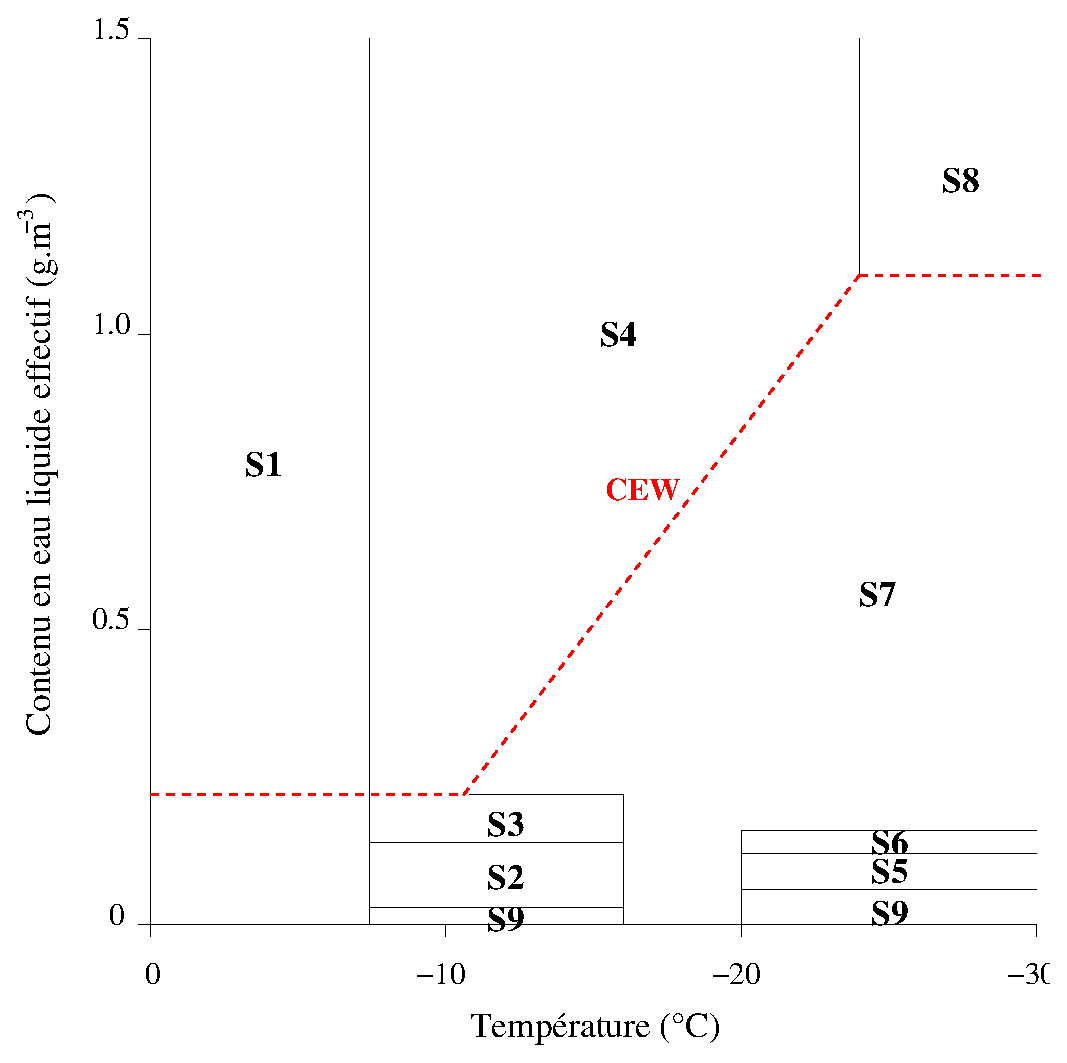
\includegraphics[width=8cm]{./EPS/saunders.eps}
  \end{center}
  \caption{\small Graphical representation of the regions of charge transfer as a function of temperature and effective liquid water content (\citet{Helsdon-2001} adapted from \citet{Saunders-1991}).}
  \label{fig:saunders}
\end{figure}
$EW$ is the effective liquid water content.
It is equal to the liquid water content times the drop collision efficiency. 
$EW$ is used instead of $LWC$ because the charge transfer mechanism is dependant on the rate of capture of the droplets rather than the liquid water content in the cloud.
The critical liquid water content, $CEW$, is defined as :
\begin{equation}
  CEW = -0.49 - 6.64 \times 10^{-2} T
\end{equation}
where $T$ is given in $^{\circ}$C.

\noindent
The equations describing each region of the graph are given in Table \ref{tab:eq_saund}.
\begin{table}[h]
  \begin{center}
  \begin{tabular}{|c|c|}
    \hline
    Equation number & Charge transfer equation\\
    \hline
    S1 & values linearly interpolated\\
    \hline
    S2 & $\delta Q = -314.40 \times EW + 7.92$\\
    \hline
    S3 & $\delta Q = 419.40 \times EW - 92.64$\\
    \hline
    S4 & $\delta Q = 20.22 \times EW + 1.36 \times T + 10.05$\\
    \hline
    S5 & $\delta Q = 2041.76  \times EW - 128.70$\\
    \hline
    S6 & $\delta Q = -2900.22 \times EW + 462.91$\\
    \hline
    S7 & $\delta Q = 3.02 - 31.76 \times EW + 26.53 \times EW^{2}$\\
    \hline
    S8 & $\delta Q = 20.22 \times EW - 22.26$\\
    \hline
    S9 & $\delta Q = 0.0$\\
    \hline
  \end{tabular}
  \end{center}
  \caption{\small Charge transfer equations from \citet{Saunders-1991}.}
  \label{tab:eq_saund}
\end{table}
In region S1, there is no laboratory results for temperature higher than -7.35$^{\circ}$C.
So, the values of $\delta Q$ at -7.35$^{\circ}$C are linearly interpolated until 0$^{\circ}$C.
At $T$ = 0$^{\circ}$C, the charge tranfer is null.
This interpolation concerns regions S1, S2, S3 and S9 :
\begin{equation}
  \begin{array}{lcl}
    \delta Q_{S1} & = & (-2.75 \times EW - 0.007) \times T \\
    \delta Q_{S3} & = & (-57.06 \times EW + 12.60) \times T \\
    \delta Q_{S2} & = & (42.78 \times EW - 1.08) \times T \\
    \delta Q_{S9} & = & 0
  \end{array}
\end{equation}

%--------------------------------------------------------
\subsubsection{Saunders and Peck (1998) parameterization}
%--------------------------------------------------------

\citet{Brooks-1997} reexamined the results of \citet{Saunders-1991} laboratory experiments, but transformed the effective liquid water content ($EW$) into the rime accretion rate ($RAR$, in g m$^{-2}$ s$^{-1}$):
$$RAR = EW \times V$$
with $V$ the relative velocity of the two particles ($x$ and $y$) experiencing collision.
In Meso-NH, the rime accretion rate is defined by:
\begin{equation}
  \begin{array}{rl}
    RAR = \rho _{air} \times r_c \times E_{cg} \times |V_{xmean} - V_{ymean}|  \mbox{ with } V_{mean} = \frac{\int _0 ^{+\infty} V(D) m(D) n(D) dD}{\int _0 ^{+\infty} m(D) n(D) dD}
  \end{array}
\end{equation}
$E_{cg}$ represents the collection efficiency of cloud droplets by graupel, and $V_{mean}$ is the mean fall speed of the considered particle.
The charge exchanged (in fC) during an elastic collision between two ice particles is the same as in the parameterization of \citet{Saunders-1991}:
\begin{equation}
  \delta q_{NI} ^{SP98} = B D ^m (\Delta v)^n \delta Q 
\end{equation}
$D$ is the diameter of the smallest particle (m), $\Delta v$ is the relative fall speed (m s$^{-1}$).
The $m$, $n$ and $B$ coefficients are the same as for \citet{Saunders-1991} (see Table \ref{tab:param_saund}).
The critical rime accretion rate ($RAR _{crit}$, in g m$^{-2}$ s$^{-1}$) is the RAR above which the biggest particle charges positively and below which it charges negatively:
\begin{equation}
  RAR_{crit} = a + b T + c T^2 + d T^3 + e T^4 + f T^5 + g T^6
\end{equation}
$a = 1.0$, $b = 7.9262 \times 10^{-2}$, $c = 4.4847 \times 10^{-2}$, $d = 7.4754 \times 10^{-3}$, $e = 5.4686 \times 10^{-4}$, $f = 1.6737 \times 10^{-5}$ et $g = 1.7613 \times 10^{-7}$.

\begin{figure}[h]
  \begin{center}
     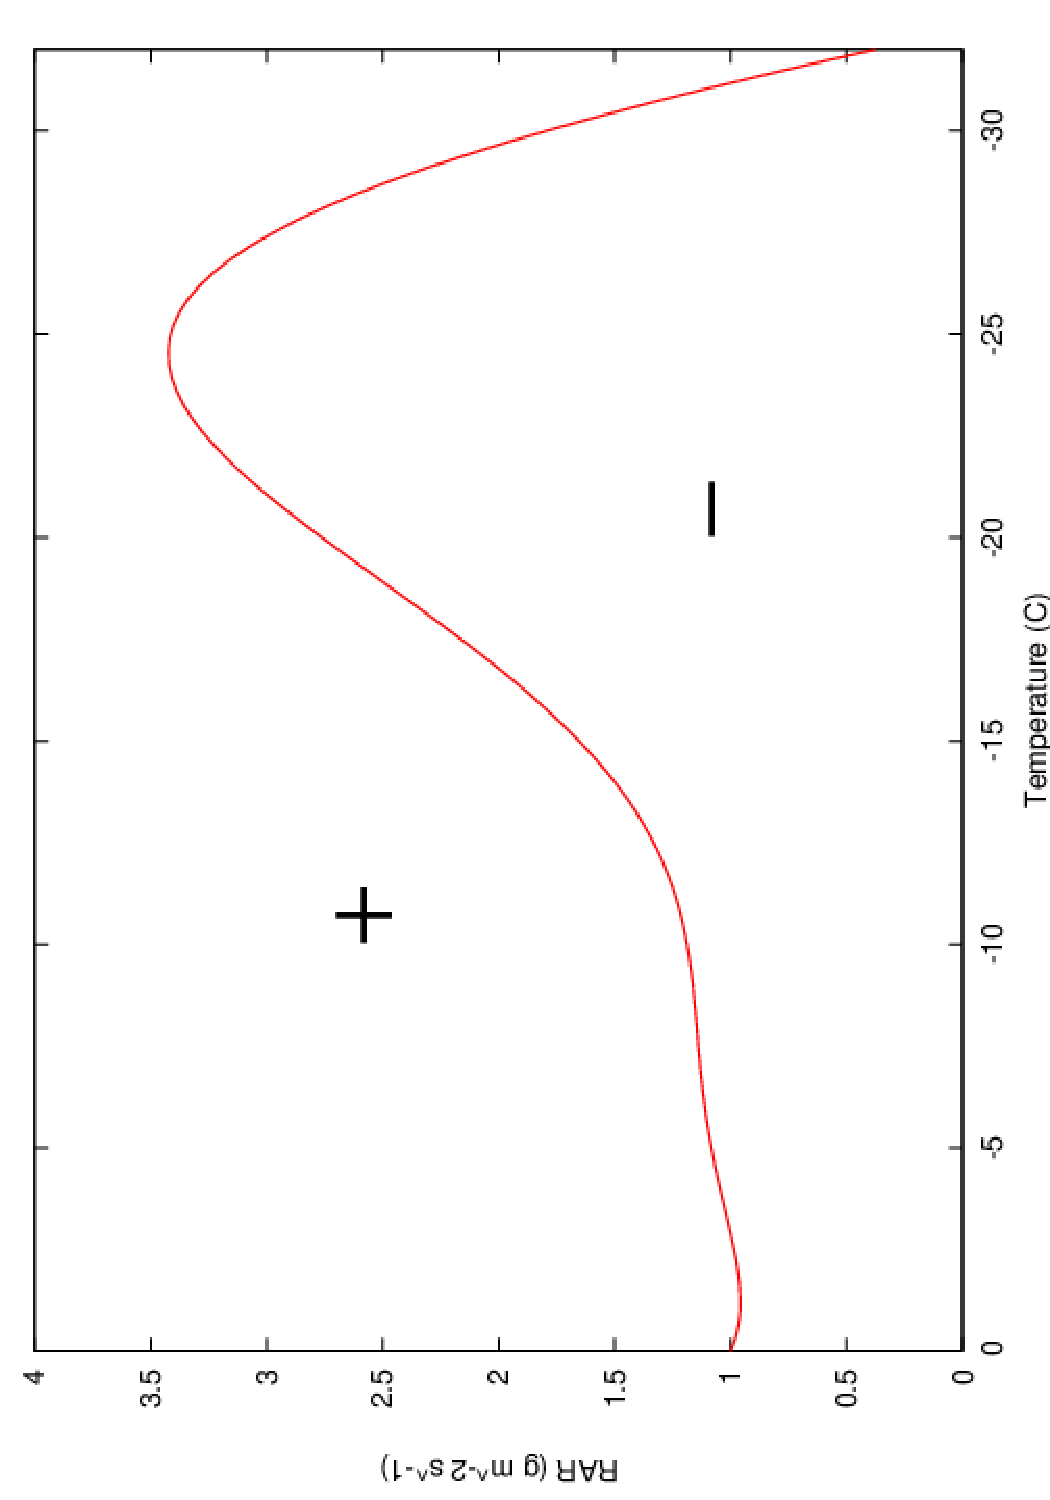
\includegraphics[angle=270,width=8cm]{./EPS/saunders_peck.pdf}
  \end{center}
  \caption{Plot of the critical rime accretion rate curve (red line) used in the \citet{Saunders-1998} noninductive ice-ice parameterization. Graupel charges positively at rime accretion rates above the curve and negatively below.}
  \label{fig:saunders_peck}
\end{figure}

The charge transfered per collision ($\delta Q$, in fC) depends on the temperature and the rime accretion rate.
Since the original equations of \citet{Saunders-1998} are only valid for temperatures between -8$^{\circ}$C and -23$^{\circ}$C, the parameterization of \citet{Saunders-1998} is adapted, partially following \citet{Mansell-2005}.

For $RAR < RAR_{crit}$, Equation (20) of \citet{Mansell-2005} is used to extend the application of the charge separation regime to $RAR$ between 0.1 and 0.3 g m$^{-2}$ s$^{-1}$. 
\begin{equation}
  \delta Q = 3.9 (RAR_{crit} - 0.1) \times \left( 4 \left[ \frac{RAR - (RAR_{crit} + 0.1)/2}{RAR_{crit} - 0.1}\right]^2 -1 \right)
\end{equation}

For $RAR > RAR_{crit}$, the original formula of \citet{Saunders-1998} is kept.
Outside the temperature range of -8$^{\circ}$C to -23$^{\circ}$C where the original \citet{Saunders-1998} scheme is strictly valid, the charging rate is linearly decreased to zero at 0(-40)$^{\circ}$C from the computed value at -8(-23)$^{\circ}$C, as suggested by \citet{Mansell-2005}.
Then for $RAR > RAR_{crit}$ and $T < -8^{\circ}$C:
\begin{equation}
  \delta Q = 6.74 RAR - 1.36 (-T) + 10.05
\end{equation}
while for $RAR > RAR_{crit}$ and $T > -8^{\circ}$C:
\begin{equation}
  \delta Q = -(6.74 RAR - 0.83) \times \frac{(T-T_t)}{8}
\end{equation}
Charging is set to 0 for $RAR < 0.1$ g m$^{-2}$ s$^{-1}$.

%----------------------------------------------------
\subsubsection{Brooks et al. (1997) parameterization}
%----------------------------------------------------

This parameterization uses the original parameterization of non-inductive charging proposed in \citet{Brooks-1997}, where the separated charge in \citet{Saunders-1991} is calculated by means the rime accretion rate $RAR$.
The critical liquid water content, $CRAR$, is defined as :
\begin{equation}
  CRAR = -1.47 - 0.2 \times T
\end{equation}

\noindent
The equations of \citet{Brooks-1997} describing each region of the graph are given in Table \ref{tab:eq_brook}.
\begin{table}[h]
  \begin{center}
  \begin{tabular}{|c|c|}
    \hline
    Equation number & Charge transfer equation\\
    \hline
    S1 & values linearly interpolated\\
    \hline
    S2 & $\delta Q = -104.8 \times RAR + 7.92$\\
    \hline
    S3 & $\delta Q = 139.8 \times RAR - 92.64$\\
    \hline
    S4 & $\delta Q = 6.74 \times RAR + 1.36 \times T + 10.05$\\
    \hline
    S5 & $\delta Q = 680.6  \times RAR - 128.70$\\
    \hline
    S6 & $\delta Q = -966.73 \times RAR + 462.91$\\
    \hline
    S7 & $\delta Q = 3.02 - 10.59 \times RAR + 10.59 \times RAR^{2}$\\
    \hline
    S8 & $\delta Q = 6.74 \times RAR - 22.26$\\
    \hline
    S9 & $\delta Q = 0.0$\\
    \hline
  \end{tabular}
  \end{center}
  \caption{\small Charge transfer equations from \citet{Brooks-1997}.}
  \label{tab:eq_brook}
\end{table}

The values of $\delta Q$ at -7.35$^{\circ}$C are linearly interpolated until 0$^{\circ}$C.
At $T$ = 0$^{\circ}$C, the charge transfer is null.
This interpolation concerns regions S1, S2, S3 and S9:
\begin{equation}
  \begin{array}{lcl}
    \delta Q_{S1} & = & (-0.9 \times RAR - 0.007) \times T \\
    \delta Q_{S3} & = & (-19.02 \times RAR + 12.60) \times T \\
    \delta Q_{S2} & = & (14.26 \times RAR - 1.08) \times T \\
    \delta Q_{S9} & = & 0
  \end{array}
\end{equation}

%-------------------------------------------------------------------------------------------------
\subsubsection{Tsenova and Mitzeva (2009) parameterization of Takahashi (1978) laboratory results}
%-------------------------------------------------------------------------------------------------

This parameterization uses the work of \citet{Tsenova-2009} where empirical equations for sign and magnitude of separated charge obtained by \citet{Takahashi-1978} are proposed. 
The sign and amplitude of the charge exchanged are expressed according to \citet{Saunders-1991}:
\begin{equation}
  \delta q_{NI} ^{T09} = B D_i ^m (\Delta v_{gi})^n \delta Q
\end{equation}

\noindent
The values of the constants $m$, $n$ and $B$ are given in Table \ref{tab:param_taka1}.
\begin{table}[h]
  \begin{center}
  \begin{tabular}{|c|c|c|c|c|}
    \hline
    Crystal size ($\mu$ m) & Situation & B & m & n \\
    \hline
    d $<$ 155            & + & 6.1  $\times$ 10$^{12}$ & 3.76 & 2.5 \\
    \hline
    155 $<$ d $\leq$ 452 & + & 5    $\times$ 10$^{5}$  & 1.90 & 2.5 \\
    \hline
    d $>$ 452            & + & 6.5                     & 0.44 & 2.5 \\
    \hline
    d $\leq$ 253         & - & 4.3  $\times$ 10$^{7}$  & 2.54 & 2.8 \\
    \hline
    d $>$ 253            & - & 2                       & 0.50 & 2.8 \\
    \hline
  \end{tabular}
  \end{center}
  \caption{\small Values of constants $B$, $m$ and $n$ proposed by \citet{Tsenova-2009} to be used in the equation of the charge transfer obtained in \citet{Takahashi-1978}.}
  \label{tab:param_taka1}
\end{table}

\noindent
(1) For $T$ $>$ -10$^{\circ}$C:
\begin{itemize}
  \item at $EW$ $<=$ 1.6 g m$^{-3}$:
\begin{eqnarray}
 \delta Q & = & 146.981 \times EW - 116.37 \times EW^{2} + 29.762 \times EW^{3}  \nonumber \\
          &   & - 0.03 \times T^{3} \times EW - 2.581 \times T - 0.0209 \times T^{3} \times EW^{3} \nonumber \\
          &   & + 0.356 \times T^{3} \times EW^{2} + 0.15 \times T^{2} + 2.918 \times T \times EW^{3} \nonumber  \\ 
          &   & - 4.215 \times T \times EW - 8.5059 
\end{eqnarray}
  \item at $EW$ $>$ 1.6 g m$^{-3}$:
\begin{eqnarray}
 \delta Q & = & 4.179 \times T - 0.0045 \times T^{2} \times EW^{2} + 0.916 \times EW^{2} \nonumber \\
          &   & - 1.333 \times T \times EW - 7.465 \times EW + 0.109 \times T \times EW^{2} \nonumber \\
          &   & + 0.0006 \times T^{2} \times EW^{3} - 0.035 \times EW^{3} + 50.845
\end{eqnarray}
\end{itemize}

\noindent
(2) For $T$ $<=$ -10$^{\circ}$C:
\begin{itemize}
  \item at $EW$ $<=$ 0.4 g m$^{-3}$:
\begin{eqnarray}
 \delta Q & = & -3.35 \times T + 95.9 \times T \times EW^{2} + 511.83 \times EW \nonumber \\
          & + & 17.45 \times T^{2} \times EW^{3} - 0.0007 \times T^{3} + 20.57 \times T \times EW \nonumber \\
          &   & + 0.165 \times T^{2} \times EW + 0.495 \times T^{3} \times EW^{3} - 0.098 \times T^{3} \times EW^{2} \nonumber  \\
          &   & +67.46 \times T \times EW^{3} - 0.107 \times T^{2} - 24.5715
\end{eqnarray}
  \item at 0.4 g m$^{-3}$ $<$ $EW$ $<=$ 3.2 g m$^{-3}$:
\begin{eqnarray}
 \delta Q & = & -1.567 \times T \times EW + 0.248 \times T \times EW^{3} + 0.01 \times T^{3} \nonumber \\
          &   & + 19.2 \times T + 0.805 \times T^{2} + 5.97 \times EW^{3} - 83.39 \times EW \nonumber \\
          &   & + 15.36 \times EW^{2} + 167.93
\end{eqnarray}
  \item at $EW$ $>$ 3.2 g m$^{-3}$:
\begin{equation}
 \delta Q = 4.213 \times T - 0.831 \times T \times EW + 0.067 \times T \times EW^{2} + 0.004 \times T^{2} \times EW + 40.964
\end{equation}
\end{itemize}

%-------------------------------------------------------------------------------------------------
\subsubsection{Tsenova and Mitzeva (2011) parameterization of Takahashi (1978) laboratory results}
%-------------------------------------------------------------------------------------------------

This parameterization uses the work of \citet{Tsenova-2011} where empirical equations for sign and magnitude of separated charge obtained by \citet{Takahashi-1978} using the rime accretion rate ($RAR$) are proposed.

\noindent
(1) For $T$ $>$ -10$^{\circ}$C:
\begin{itemize}
  \item at $RAR$ $<=$ 12.8 g m$^{-2}$ s$^{-1}$:
\begin{eqnarray}
 \delta Q & = & 18.37 \times RAR - 1.82 \times RAR^{2} - 0.06 \times RAR^{3} \nonumber \\
          &   & - 0.004 \times T^{3} \times RAR - 2.581 \times T + 0.0004 \times T^{3} \times RAR^{3} \nonumber \\
          &   & + 0.006 \times T^{3} \times RAR^{2} + 0.15 \times T^{2} + 0.006 \times T \times RAR^{3} \nonumber \\ 
          &   & - 0.53 \times T \times RAR - 8.5059 
\end{eqnarray}
  \item at $RAR$ $>$ 12.8 g m$^{-2}$ s$^{-1}$:
\begin{eqnarray}
 \delta Q & = & 4.179 \times T - 0.00007 \times T^{2} \times RAR^{2} + 0.01 \times RAR^{2} \nonumber \\
          &   & - 0.17 \times T \times RAR - 0.93 \times RAR + 0.002 \times T \times RAR^{2} \nonumber \\
          &   & + 0.000001 \times T^{2} \times RAR^{3} - 0.00007 \times RAR^{3} + 50.845
\end{eqnarray}
\end{itemize}

\noindent
(2) For $T$ $<=$ -10$^{\circ}$C:
\begin{itemize}
  \item at $RAR$ $<=$ 3.2 g m$^{-2}$ s$^{-1}$:
\begin{eqnarray}
 \delta Q & = & -3.35 \times T + 1.5 \times T \times RAR^{2} + 63.98 \times RAR \nonumber \\
          &   & + 0.03 \times T^{2} \times RAR^{3} - 0.0007 \times T^{3} + 2.57 \times T \times RAR \nonumber \\
          &   & + 0.02 \times T^{2} \times RAR + 0.001 \times T^{3} \times RAR^{3} - 0.002 \times T^{3} \times RAR^{2} \nonumber \\
          &   & + 0.13 \times T \times RAR^{3} - 0.107 \times T^{2} - 24.5715
\end{eqnarray}
  \item at 3.2 g m$^{-2}$ s$^{-1}$ $<$ $RAR$ $<=$ 25.6 g m$^{-2}$ s$^{-1}$:
\begin{eqnarray}
 \delta Q & = & -0.2 \times T \times RAR + 0.0005 \times T \times RAR^{3} + 0.01 \times T^{3} \nonumber \\
          &   & + 19.2 \times T + 0.805 \times T^{2} + 0.01 \times RAR^{3} - 10.42 \times RAR \nonumber \\
          &   & + 0.24 \times RAR^{2} + 167.93
\end{eqnarray}
  \item at $RAR$ $>$ 25.6 g m$^{-2}$ s$^{-1}$:
\begin{equation}
 \delta Q = 4.213 \times T - 0.1 \times T \times RAR + 0.001 \times T \times RAR^{2} + 0.0005 \times T^{2} \times RAR + 40.964
\end{equation}
\end{itemize}


\paragraph{Limitations of the charge exchanged per collision}

As in \citet{Mansell-2005}, the charge exchanged per rebounding collision $\delta q$ is limited to prevent unreasonable charging rate.
Based on \citet{Keith-1990}, it is assumed that the charging rate of the pristine ice crystal with $D_{max}$ $\sim$ 100 $\mu$m is the most limiting one, that is 30(10) fC per collision with graupel(aggregate) particles.
We take a larger value (100 fC) for the graupel-snow collisions because it corresponds roughly to an average of the saturation levels when the particle sizes reach $\sim$ 1 mm (see \citet{Keith-1990} or Fig. 3.13 in \citet{MacGorman-Rust}).
This limitation is introduced in the computation of the bulk charging rates which result from an integration over the size spectrum of the ice particles.


%++++++++++++++++++++++++++++++++
\subsection{Inductive mechanism}
%++++++++++++++++++++++++++++++++

Laboratory studies conducted by \citet{Aufdermaur-1972} have shown that in the presence of an electric field stronger than a few kV m$^{-1}$ collisions between particles would lead to significant charge exchange. 
Drop-drop inductive charging is not considered because most of the time the two colliding particles end up with a single bigger drop. 
Concerning ice-ice inductive charging, the short duration and small size of the contact zone and the low ice electrical conductivity do not allow for a substantial charge exchange when ice particles collide \citep{Illingworth-1985a}. 
Therefore only bouncing collisions between graupel and droplets are likely needed to be taken into account. 
Even if the rate of rebounding collisions is low compared to the rate of sticking collisions, the amount of charge separated is important. 
The inductive charging rate parameterization follows the expression given by \citet{Ziegler-1991}:
\begin{equation}
  \frac{\partial \rho_g (D_g)}{\partial t} = \frac{\pi}{4} E_{cg} E_r D_g ^2 V(D_g) N_c \alpha \left[ \frac{\pi ^3}{2} D_c ^2 \epsilon E_z \cos(\theta) - \frac{\pi ^2}{6}\rho_g(D_g) \frac{D_c ^2}{D_g ^2} \right]
\end{equation}
where $E_{cg}$ is the graupel-droplets collision efficiency, $E_r$ the rebound probability, and $E_z$ the vertical component of the electric field. 
$\epsilon$ is the permittivity of air. 
$\rho _g$ is the graupel charge density, $D_c$ the cloud droplets diameter, and $D_g$ the graupel diameter. 
$V$ is the fall speed of graupel, and $N_c$ is the number concentration of cloud droplets. 
The second term of the expression accounts for a preexisting charge polarity of the graupel. 
Assuming that grazing collisions are the most efficient ones, $\alpha$ is the fraction of droplets experiencing grazing trajectories, and $\cos(\theta)$ is the mean cosine collision angle. 
$E_r$, $\alpha$ and $\cos(\theta)$ are set to 0.1, 0.07 and 0.2, respectively, as suggested by \citet{Ziegler-1991}.


%%%%%%%%%%%%%%%%%%%%%%%%%%%%%%%%%%%%%%%%%%%%%%%%%%%%%%%
\section{Charge transfers associated to mass transfers}
\label{sec:micro}
%%%%%%%%%%%%%%%%%%%%%%%%%%%%%%%%%%%%%%%%%%%%%%%%%%%%%%%

Once charges are separated by the non-inductive process, they can be exchanged between the different hydrometeor categories during the microphysical processes.

\begin{figure}[h]
  \begin{center}
     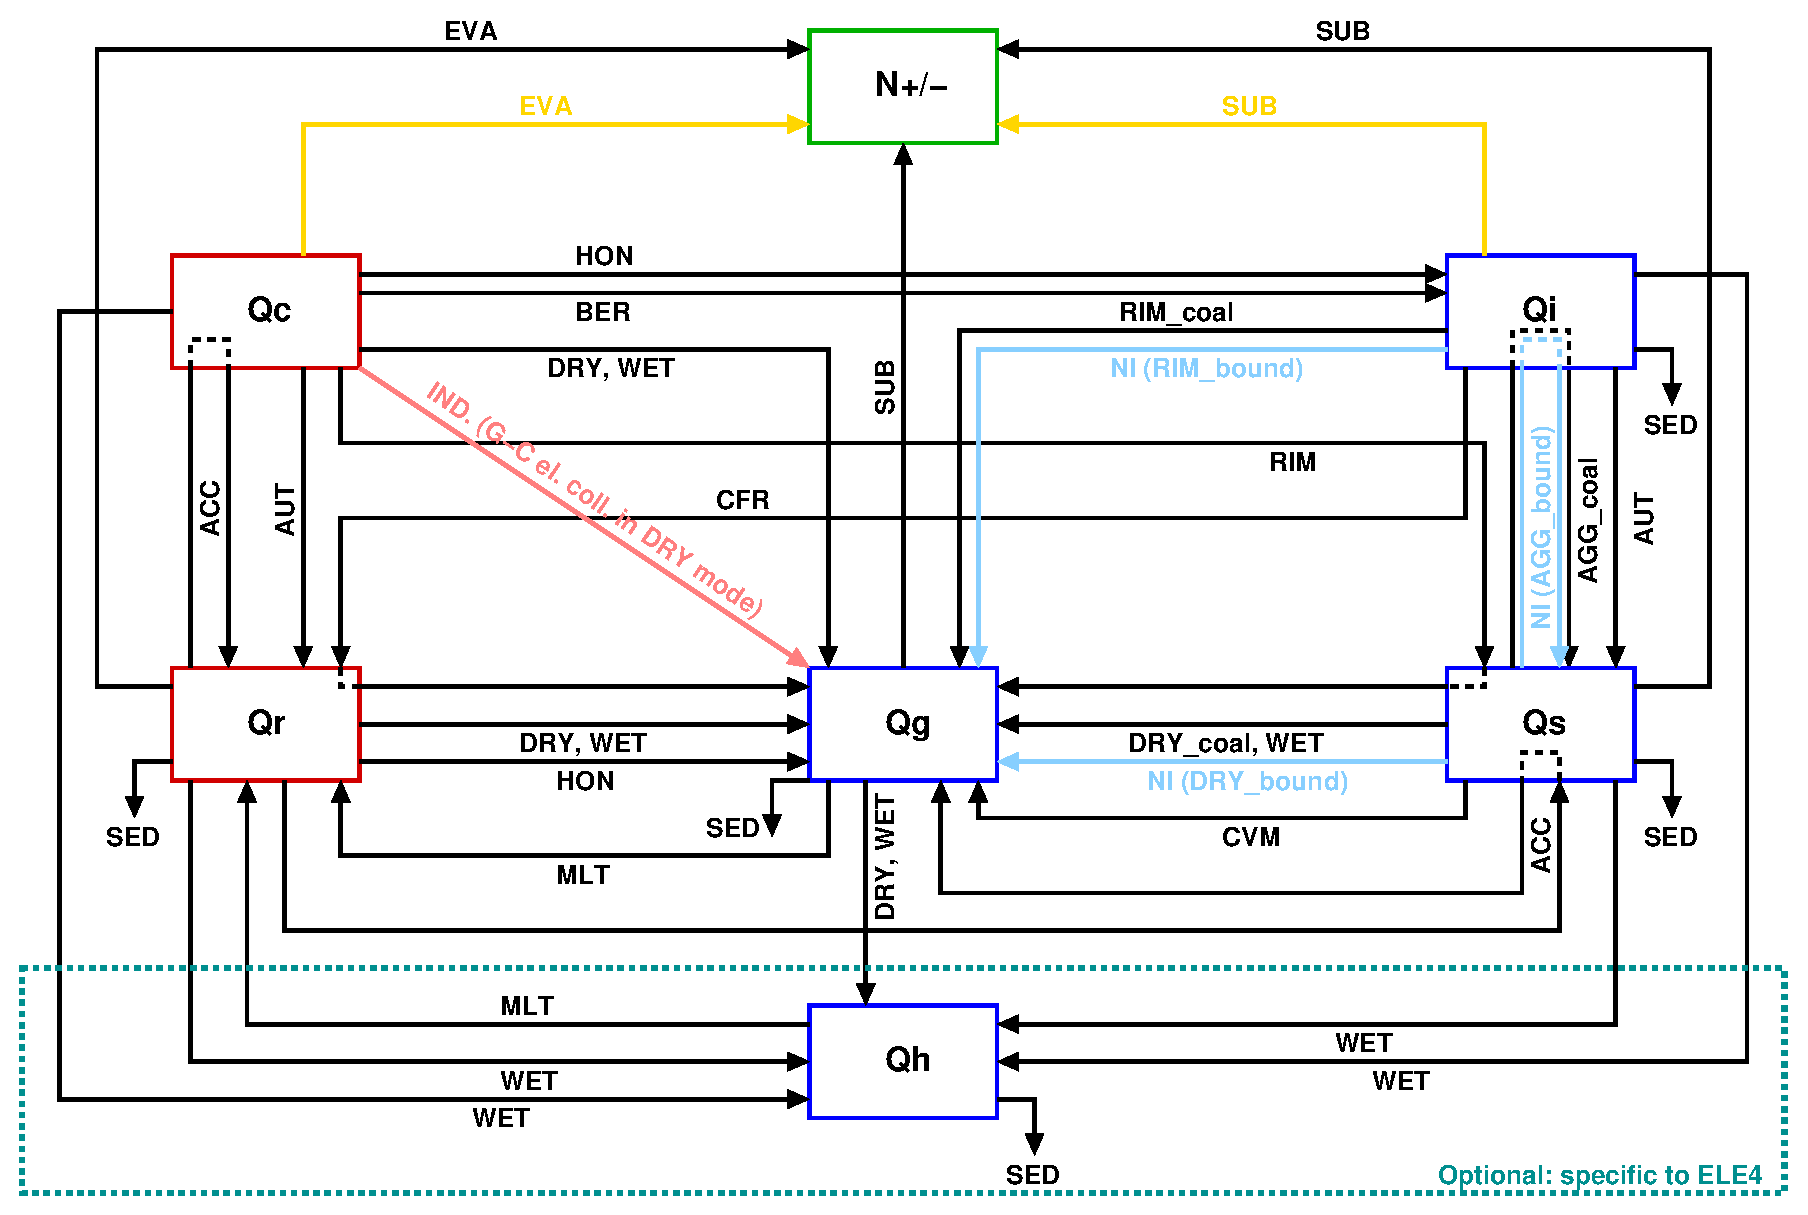
\includegraphics[width=16cm]{./EPS/charge_transfer.eps}
  \end{center}
  \caption{Diagram of the electric charge transfers. Black, light blue and pink lines represent charge transfers associated to mass transfers, to the non-inductive mechanisms, and to the inductive mechanism, respectively. The yellow lines show the electric charge transfers treated as an ajustement in ice\_adjust\_elec.f90. Ion attachment to hydrometeors is not represented in this diagram.}
  \label{fig:transfer}
\end{figure}

Similarly to the microphysical scheme, the rate of charge exchanged during mass transfer follows:
\begin{equation}
  QYCOLXZ = \int_0 ^{+ \infty} \left\{
            \int_0 ^{+ \infty} K(D_x , D_y) q_y n_y (D_y) dD_y \right\} n_x (D_x) dD_x
\end{equation}
The kernel $K$ can be written:
\begin{equation}
  K(D_x , D_y) = \frac{\pi}{4} (D_x + D_y)^2 |v_x (D_x) - v_y (D_y)| E_{xy}
\end{equation}
$E_{xy}$ is the collection efficiency.

%+++++++++++++++++++++++++
\subsection{Sedimentation}
%+++++++++++++++++++++++++

For precipitating particles (rain, snow, graupel and hail, then X = R, S, G and H), the sedimentation rate of charge density follows:
\begin{equation}
  QSEDX = \frac{\partial}{\partial z} \left[ \left( \frac{\rho _{00}}{\rho _{dref}} \right) ^{0.4} c_x e_x C_x G(d_x + f_x) \lambda ^{x - (d_x + f_x)} \right]
\end{equation}
For pristine ice:
\begin{equation}
  QSEDI = \frac{\partial}{\partial z} \left[ \left( \frac{\rho _{00}}{\rho _{dref}} \right) ^{0.4} c_i e_i N_i G(d_i + f_i) \left( \frac{\rho _{dref} r_i}{a_i N_i G(b_i)} \right) ^{\frac{d_x + f_x}{b_x}} \right]
\end{equation}

%++++++++++++++++++++++++++
\subsection{Warm processes}
%++++++++++++++++++++++++++

\paragraph{Autoconversion}

\begin{equation}
  QCAUTR = q_c \frac{RCAUTR}{r_c}
\end{equation}


\paragraph{Accretion}

\begin{equation}
  QCACCR = q_c \frac{RCACCR}{r_c}
\end{equation}


\paragraph{Evaporation and condensation of rain}

\begin{equation}
  QREVAV = q_r \frac{RREVAV}{r_r} 
\end{equation}
The charge released during rain evaporation is transfered to the ions categories following:
\begin{eqnarray}
  n_+ &=& n_+ + QREVAV / e \quad {\rm if} \quad QREVAV > 0 \\
  n_- &=& n_- - QREVAV / e \quad {\rm if} \quad QREVAV < 0
\end{eqnarray}

%++++++++++++++++++++++++++
\subsection{Ice nucleation}
%++++++++++++++++++++++++++

\paragraph{Heterogeneous nucleation}

It is considered there is no charge exchanged during this mass transfer.


\paragraph{Homogeneous nucleation}

For temperatures colder than -35$^{\circ}$C, cloud droplets spontaneously freeze and are transfered to the ice crystals category.
If $P \approx J_{HOM}(T) V \Delta t$ is the probability for a cloud droplet with volume $V$ to freeze during $\Delta$t, the charge exchanged during this process can be computed in the same manner as for the microphysical process:
\begin{eqnarray}
  QCHONI & = & \int_0 ^{+ \infty} q_c P M_c (D_c) dD_c \nonumber \\
         & = & \frac{\pi}{6} J_{HOM} \rho r_c \frac{e_c}{a_c} \frac{G(f_c + 3)}{G(b_c)} \lambda ^{b_c - (f_c + 3)}
\end{eqnarray}
a$_{c}$ is the proportionality factor in the mass-diameter relation ($a_c = 1000 \times \frac{\pi}{6}$). 
Moments are computed using: $\lambda _{c}$ = 1.1 $\times$ 10$^{5}$ m$^{-3}$, $\alpha _{c}$ = 3 and $\nu _{c}$ = 1.


\paragraph{Homogeneous nucleation}

For temperatures lower than -35$^{\circ}$C, raindrops freeze spontaneously.
\begin{eqnarray}
  QRHONG & = & q_r H(T_t - 35) \nonumber \\
         & = & q_r \frac{RRHONG}{r_r}
\end{eqnarray}

%+++++++++++++++++++++++++++++++++++++
\subsection{Bergeron-Findeisen effect}
%+++++++++++++++++++++++++++++++++++++

\begin{equation}
  QCBERI = q_c \frac{RCBERI}{r_c}
\end{equation}
However, the charge exchanged during this process is too high.
Then QCBERI is reduced to 1\% of its value.

%++++++++++++++++++++++++++++++++++++++++++++++++++++++
\subsection{Water vapor deposition on snow and graupel}
%++++++++++++++++++++++++++++++++++++++++++++++++++++++

\begin{eqnarray}
  QSSUBV &=& q_s \frac{RSSUBV}{r_s} \\
  QGSUBV &=& q_g \frac{RGSUBV}{r_g}
\end{eqnarray}
RSSUBV and RGSUBV are the negative part of the mass transfer rate during vapor deposition.

The charge released during the graupel/snow ($x = G/S$) sublimation is transfered to the ions categories following:
\begin{eqnarray}
  n_+ &=& n_+ + \frac{QxSUBV}{e}  \mbox{ if } QxSUBV > 0 \\
  n_- &=& n_- - \frac{QxSUBV}{e}  \mbox{ if } QxSUBV < 0
\end{eqnarray}

%++++++++++++++++++++++++++++++++++++++++++++++++++++++++++++++++
\subsection{Autoconversion of pristine ice and formation of snow}
%++++++++++++++++++++++++++++++++++++++++++++++++++++++++++++++++

\begin{equation}
  QIAUTS = q_i \frac{RIAUTS}{r_i}
\end{equation}

%+++++++++++++++++++++++++++++++++++++++++++++++++++++++++++++
\subsection{Contact freezing of rain and formation of graupel}
%+++++++++++++++++++++++++++++++++++++++++++++++++++++++++++++

This is a 3-species mechanism.
The collision between ice crystal and raindrop produces frozen drops.
If the pristine ice fall speed can be neglected compared to the raindrop fall speed, then the charge lost by raindrops is:
\begin{eqnarray}
  QRCFRIG &=& \int_0 ^{+ \infty} \left[ \int_0 ^{+ \infty}
    K(D_r , D_i) n_r (D_r) q_r (D_r) dD_r \right] n_i (D_i) dD_i \nonumber \\
          &=& \frac{\pi}{4} C_r N_i c_r e_r
              \left( \frac{\rho _{00}}{\rho _{dref}} \right) ^{0.4}
              G_r (d_r + f_r + 2) \lambda _r ^{x_r - (d_r + f_r + 2)}
\end{eqnarray}
And the charge lost by pristine ice is:
\begin{eqnarray}
  QICFRRG &=& \int_0 ^{+ \infty} \left[ \int_0 ^{+ \infty}
    K(D_r , D_i) n_i (D_i) q_i (D_i) dD_i \right] n_r (D_r) dD_r \nonumber \\
          &=& q_i \frac{\pi}{4} C_r \lambda _r ^{x_r} c_r
              \left( \frac{\rho _{00}}{\rho _{dref}} \right) ^{0.4}
              G_r (d_r + 2) \lambda _r ^{d_r + 2} \nonumber \\
          &=& q_i \frac{RICFRRG}{r_i}
\end{eqnarray}

%+++++++++++++++++++++++++++++++++++++++++++++++
\subsection{Aggregation of pristine ice on snow}
%+++++++++++++++++++++++++++++++++++++++++++++++

\begin{equation}
  QIAGGS = QIAGGS_{bound} + QIAGGS_{coal}
\end{equation}


\paragraph{Case with coalescence}

\begin{equation}
  QIAGGS_{coal} = \int_0 ^{+ \infty} \left\{\int_0 ^{+ \infty} \frac{\pi}{4} (D_i + D_s)^2 |v_i (D_i) - v_s (D_s)| E_{is} q_i n_i (D_i) dD_i \right\} n_s (D_s) dD_s \nonumber
\end{equation}
The ice-snow collection efficiency takes the form: $E_{is} = 0.25 \exp[0.005(T - T_t)]$.
The pristine ice diameter (fall speed) can be neglected compared to the snow diameter (fall speed):
\begin{eqnarray}
  QIAGGS_{coal} &=& \int_0 ^{+ \infty} \left\{\int_0 ^{+ \infty} \frac{\pi}{4} D_s^2 v_s (D_s) E_{is} q_i n_i (D_i) dD_i \right\} n_s (D_s) dD_s \nonumber \\
                &=& q_i \frac{RIAGGS}{r_i}
\end{eqnarray}


\paragraph{Case with elastic collision}

If ice crystals and snow particles experience elastic collisions, this is considered as part of the non-inductive mechanism.
The same approximations about diameter and fall speed as in the case with coalescence can be done.
\begin{eqnarray}
  QIAGGS_{boun} &=& \int_0 ^{+ \infty} \left\{\int_0 ^{+ \infty} \frac{\pi}{4} (D_i + D_s)^2 |v_i (D_i) - v_s (D_s)| (1 - E_{is}) q_i n_i (D_i) dD_i \right\} n_s (D_s) dD_s \nonumber \\
                &=& \frac{\pi}{4} (1 - E_{is}) c_s \left( \frac{\rho _{00}}{\rho _{dref}} \right) ^{0.4}
			\int_0 ^{+ \infty} D_s ^{(2 + d_s)} \left[ \int_0 ^{+ \infty} q_i n_i (D_i) dD_i \right] n_s (D_s) dD_s
\end{eqnarray}
Different parameterizations are available for this process.\\

\begin{enumerate}
  \item {\bf \textsc{Helsdon and Farley (1987)}}

For a snow-ice collision, $\delta q_{is} = 2.10^{-15}$C, then:
\begin{eqnarray}
  QIAGGS_{boun} &=& \frac{\pi}{4} (1 - E_{is}) c_s
                \left( \frac{\rho _{00}}{\rho _{dref}} \right) ^{0.4}
                \delta q_{is} N_i
                \int_0 ^{+ \infty} D_s ^{(2 + d_s)}  n_s (D_s) dD_s 
                \nonumber \\
                &=& \frac{1 - E_{is}}{E_{is}} RIAGGS 
                \frac{\delta q_{is}}{r_i} N_i
\end{eqnarray}

 \item {\bf\textsc{Takahashi (1978)}}

\begin{eqnarray}
  QIAGGS_{boun} &=& \frac{\pi}{4} (1 - E_{is}) c_s
                \left( \frac{\rho _{00}}{\rho _{dref}} \right) ^{0.4}
                \int_0 ^{+ \infty} D_s ^{(2 + d_s)}
                \left[ \int_0 ^{+ \infty} f(T,LWC) \times \right. \nonumber \\
                & & \left. {\rm Min} \left( 10, 5
                    \left( \frac{D_i}{D_0} \right) ^2
                    \frac{|v_s - v_i|}{v_0} \right) n_i (D_i) dD_i \right]
                n_s (D_s) dD_s \nonumber
\end{eqnarray}
It is assumed that $v_i \ll v_s$:
\begin{eqnarray}
  QIAGGS_{boun} &=& \frac{\pi}{4} (1 - E_{is}) c_s
                \left( \frac{\rho _{00}}{\rho _{dref}} \right) ^{0.4}
                f(T,LWC)
                \int_0 ^{+ \infty} D_s ^{(2 + d_s)}
                \left[ \int_0 ^{+ \infty} \times \right. \nonumber \\
                & & \left. {\rm Min} \left( 10, 5
                    \left( \frac{D_i}{D_0} \right) ^2
                    \frac{|v_s - v_i|}{v_0} \right) N_i g(D_i) dD_i \right]
                n_s (D_s) dD_s  \nonumber \\
                &=& \frac{\pi}{4} (1 - E_{is}) 
                \left( \frac{\rho _{00}}{\rho _{dref}} \right) ^{0.4}
                c_s N_i N_s f(T,LWC) \times \nonumber \\ 
                & & {\rm Min} \left[ 10 G_s (2 + d_s) \lambda _s ^{-(2 + d_s)},
                  \frac{5 c_s}{D_0 ^2 v_0} 
                  \left( \frac{\rho _{00}}{\rho _{dref}} \right) ^{0.4}
                  G_i (2) \lambda _i ^{-2} G_s (2 + 2d_s)
                  \lambda ^{-(2 + 2d_s)} \right] \nonumber \\
\end{eqnarray}

  \item {\bf \textsc{Gardiner et al. (1985)}}

\begin{eqnarray}
  QIAGGS_{boun} &=& \frac{\pi}{4} (1 - E_{is}) c_s
                \left( \frac{\rho _{00}}{\rho _{dref}} \right) ^{0.4}
                \int_0 ^{+ \infty} D_s ^{(2 + d_s)} \nonumber \\
                & & \left[ \int_0 ^{+ \infty} 73 D_i ^4 (v_s - v_i)^3
                  \delta L f(\tau) n_i (D_i) dD_i \right]
                n_s (D_s) dD_s \nonumber
\end{eqnarray}
Since $v_i \ll v_s$ :
\begin{equation}
  QIAGGS_{boun} = \frac{\pi}{4} (1 - E_{is})
                \left( \frac{\rho _{00}}{\rho _{dref}} \right) ^{4 \times 0.4}
                c_s ^4 N_i C_s G_i (4) \lambda _i ^{-4}
                G_s (2 + 4d_s) \lambda _s ^{x_s - (2 + 4d_s)}
                73 \delta L f(\tau) \times 10^{15}
\end{equation}

  \item {\bf \textsc{Saunders et al. (1991), Saunders et Peck (1998), Brooks et al. (1997), Tsenova and Mitzeva (2009, 2011)}}

\begin{eqnarray}
  QIAGGS_{boun} &=& \frac{\pi}{4} (1 - E_{is}) c_s
                \left( \frac{\rho _{00}}{\rho _{dref}} \right) ^{0.4}
                \int_0 ^{+ \infty} D_s ^{(2 + d_s)} \nonumber \\
                & & \left[ \int_0 ^{+ \infty} B D_i ^a |v_s - v_i | ^b \delta Q
                  N_i g(D_i) dD_i \right] n_s (D_s) dD_s \nonumber
\end{eqnarray}
$v_i \ll v_s$ and $q$ only depends on temperature and liquid water content:
\begin{eqnarray}
  QIAGGS_{boun} &=& \frac{\pi}{4} (1 - E_{is}) 
                  \left( \frac{\rho _{00}}{\rho _{dref}} \right)^{0.4(1 + b_s)}
                  c_s ^{1 + b_s} N_i C_s G_i (a_i) \lambda _i ^{a_i}
                  \nonumber \\
                & & G_s (2 + (1 + b_s) d_s ) 
                  \lambda _s ^{x_s - 2 - (1 + b_s)d_s} B \delta Q
\end{eqnarray}

\end{enumerate}

%++++++++++++++++++++++++++++++++
\subsection{Riming of aggregates}
%++++++++++++++++++++++++++++++++

During the riming of aggregates, cloud droplets lose charge at rate:
\begin{eqnarray}
  QCRIMS &=& \int_0 ^{+ \infty} \left[ \int_0 ^{+ \infty}
             \frac{\pi}{4} (D_s + D_c)^2 |v_s - v_c| E_{cs} q_c n_c (D_c) dD_c
             \right] n_s (D_s) dD_s \nonumber \\
         &=& q_c \frac{RCRIMS}{r_c}
\end{eqnarray}
We assume: $v_i \ll v_s$, $D_i \ll D_s$, and $E_{cs}$ = 1.
It is also hypothesized that conversion of aggregates into graupels may occur for riming aggregates of size larger than $D_{cs} ^{lim}$ = 7 mm \citep{Farley-1989}.
Thus the charge gained by aggregates during their growth by riming takes the form:
\begin{eqnarray}
  QCRIMSS &=& \int_0 ^{D_s ^{lim}} \left[ \int_0 ^{+ \infty}
              \frac{\pi}{4} (D_s + D_c)^2 |v_s - v_c| E_{cs} q_c n_c (D_c) dD_c
              \right] n_s (D_s) dD_s \nonumber \\
          &=& \frac{\pi}{4} 
              \left( \frac{\rho _{00}}{\rho _{dref}} \right)^{0.4}
              c_s C_s \lambda ^{x_s} q_c M(S + d_s ; D_s ^{lim}) \nonumber \\
          &=& q_c \frac{RCRIMSS}{r_c}
\end{eqnarray}
If $D_s > D_{cs} ^{lim}$:
\begin{eqnarray}
  QCRIMSG &=& \int_0 ^{+ \infty} \left[ \int_{D_s ^{lim}} ^{+ \infty}
              \frac{\pi}{4} (D_s + D_c)^2 |v_s - v_c| E_{cs} q_c n_c (D_c) dD_c
              \right] n_s (D_s) dD_s \nonumber \\
          &=& QCRIMS - QCRIMSS \nonumber \\
          &=& \frac{q_c}{r_c} (RCRIMS - RCRIMSS)
\end{eqnarray}

%++++++++++++++++++++++++++++++++++++++++++++
\subsection{Accretion of rain and aggregates}
%++++++++++++++++++++++++++++++++++++++++++++

As for the riming of cloud droplets, it is postulated that the collection of small raindrops do not change the structure of an aggregate but larger colliding raindrops reshape it as a graupel.
The rate of charge exchanged during the collection of raindrops by snow has the form:
\begin{equation}
  QRACCS = \int_0 ^{+ \infty} \left[ \int_0 ^{+ \infty}
           \frac{\pi}{4} (D_s + D_r)^2 |v_r - v_s| E_{rs} q_r n_r (D_r) dD_r
           \right] n_s (D_s) dD_s \nonumber
\end{equation}
It is assumed that $E_{rs}$ = 1.
Furthermore, as both raindrops and aggregates have significant fall speeds, it is not easy to solve the integrals.
They are tabulated in function of $\lambda _{r}$ et $\lambda _{s}$.
\begin{eqnarray}
  QRACCS & = & \int_0 ^{+ \infty} \left[ \int_0 ^{+ \infty}
           E_{rs} \frac{\pi}{4} 
           \left( \frac{\rho _{00}}{\rho _{dref}} \right)^{0.4}
           (D_r + D_s)^2 |c_r D_r ^{d_r} - c_s D_s ^{d_s}| q_r N_r g(D_r) dD_r
           \right] \times \nonumber \\
         &   & N_s g(D_s) dD_s \nonumber
\end{eqnarray}
We define:
\begin{eqnarray}
  \Delta vq_{rs}(\lambda _s, \lambda _r) & = &
    \Lambda q(\lambda _s, \lambda _r)^{-1} \int_0 ^{+ \infty} \left[
      \int_0 ^{+ \infty} E_{rs} (D_r + D_s)^2 
      |c_r D_r ^{d_r} - c_s D_s ^{d_s}| D_r ^{f_r} g(D_r , \lambda _r)dD_r 
    \right] \times \nonumber \\
                                         &   & g(D_s , \lambda _s) dD_s \nonumber
\end{eqnarray}
with:
\begin{eqnarray}
  \Lambda q(\lambda _s, \lambda _r) &=& \int_0 ^{+ \infty} \left[ 
    \int_0 ^{+ \infty} (D_r + D_s)^2 D_r ^{f_r} g(D_r , \lambda _r) dD_r
    \right] g(D_s , \lambda _s) dD_s \nonumber \\
   &=& M_r(2 + f_r) + M_s(2)M(f_r) + 2 M_s(1) M_r(1 + f_r) \nonumber \\
   &=& G_r(2 + f_r) \lambda _r ^{-(2 + f_r)} + G_s(2) G(f_r) \lambda _s ^{-2} 
       \lambda _r ^{-f_r} \nonumber \\
   & & + 2 G_s(1) G_r(1 + f_r) \lambda _s ^{-1} 
       \lambda _r ^{-(1+f_r)} 
\end{eqnarray}
Since $q_r (D_r) = e_r D_r ^{f_r}$:
\begin{equation}
  QRACCS = \frac{\pi}{4} \left( \frac{\rho _{00}}{\rho _{dref}} \right)^{0.4}
           N_r N_s e_r \Delta vq_{rs}(\lambda _s, \lambda _r)
           \Lambda q(\lambda _s, \lambda _r)
\end{equation}

\noindent
\underline{If $D_r < D_{r} ^{lim}$}, the structure of the aggregates is not changed:
\begin{eqnarray}
  QRACCSS &=& \int_0 ^{+ \infty} \left[ \int_0 ^{D_r ^{lim}}
            \frac{\pi}{4} (D_r + D_s)^2 |v_r - v_s| E_{rs} q_r (D_r) 
            n_r (D_r) dD_r
            \right] n_s (D_s) dD_s \nonumber \\
          &=& \frac{\pi}{4} 
              \left( \frac{\rho _{00}}{\rho _{dref}} \right)^{0.4}
              N_s N_r e_r \Lambda q(\lambda _s, \lambda _r)
              \Delta vq_{rss}(\lambda _s, \lambda _r)
\end{eqnarray}
with :
\begin{eqnarray}
  \Delta vq_{rss}(\lambda _s, \lambda _r) & = &
    \Lambda q(\lambda _s, \lambda _r)^{-1} \int_0 ^{+ \infty} \left[
      \int_0 ^{D_r ^{lim}} E_{rs} (D_r + D_s)^2 
      |c_r D_r ^{d_r} - c_s D_s ^{d_s}| D_r ^{f_r} g(D_r , \lambda _r)dD_r 
    \right] \times \nonumber \\
      &  & g(D_s , \lambda _s) dD_s
\end{eqnarray}

\noindent
\underline{If $D_r > D_{r} ^{lim}$}, the structure of the aggregates is turned into graupel.
The rate of charge transfered from rain to graupel is:
\begin{equation}
  QRACCSG = QRACCS - QRACCSS
\end{equation}
Since $q_x (D_x) = e_x D_x ^{f_x}$, $n_x (D_x) = N_x g(D_x) = C_x \lambda ^{x_x} g(D_x)$ and $v_{x}(D_x) =  \left( \frac{\rho _{00}}{\rho _{dref}} \right)^{0.4} c_x D_x ^{d_x}$, with $x$ = $r$ or $s$, the charge lost by aggregates follows:
\begin{eqnarray}
  QSACCRG &=& \int_{D_r ^{lim}} ^{+ \infty} \left[ \int_0 ^{+ \infty} 
              \frac{\pi}{4} E_{rs} (D_r + D_s)^2 |v_r (D_r) - v_s (D_s)|
              q_s (D_s) n_s (D_s) dD_s \right] n_r (D_r) dD_r \nonumber \\
          &=& \frac{\pi}{4} 
              \left( \frac{\rho _{00}}{\rho _{dref}} \right)^{0.4}
              N_s N_r e_s
              \Lambda q(\lambda _s, \lambda _r)
              \Delta vq_{rs}(\lambda _s, \lambda _r)
\end{eqnarray}
with:
\begin{eqnarray}
  \Delta vq_{rss}(\lambda _s, \lambda _r) & = &
    \Lambda q(\lambda _s, \lambda _r)^{-1} \int_{D_r ^{lim}} ^{+ \infty}
    \left[ \int_0 ^{+ \infty}  E_{rs} (D_r + D_s)^2 
       |c_r D_r ^{d_r} - c_s D_s ^{d_s}| D_s ^{f_s}  g(D_s , \lambda _s) dD_s
       \right] \times \nonumber \\
       &  & g(D_r , \lambda _r)dD_r 
\end{eqnarray}
\begin{eqnarray}
  \Lambda q(\lambda _s, \lambda _r) &=& \int_0 ^{+ \infty} \left[ 
    \int_0 ^{+ \infty} (D_r + D_s)^2 D_s ^{f_s} g(D_s , \lambda _s) dD_s
    \right] g(D_r , \lambda _r) dD_r \nonumber \\
   &=& M_s(2 + f_s) + M_r(2)M(f_s) + 2 M_r(1) M_s(1 + f_s) \nonumber \\
   &=& G_s(2 + f_s) \lambda _s ^{-(2 + f_s)} + G_r(2) G(f_s) \lambda _r ^{-2} 
       \lambda _s ^{-f_s} \nonumber \\
   & & + 2 G_r(1) G_s(1 + f_s) \lambda _r ^{-1} 
       \lambda _s ^{-(1+ f_s)}
\end{eqnarray}

%+++++++++++++++++++++++++++++++++
\subsection{Dry growth of graupel}
%+++++++++++++++++++++++++++++++++

The charge grained by graupel during their dry growth by collection processes contains the sum of charge gained by graupel during the individual accretion processes that is:
\begin{equation}
  QDRYG = QCDRYG + QRDRYG + QIDRYG + QSDRYG
\end{equation}

\paragraph{Dry growth of graupel by collection of cloud droplets}

\begin{eqnarray}
  QCDRYG &=& \int_0 ^{+ \infty} \left[ \int_0 ^{+ \infty}
             K(D_c , D_g) q_c (D_c) n_c (D_c) dD_c \right]
             n_g (D_g) dD_g \nonumber \\
         &=& q_c \frac{RCDRYG}{r_c}
\end{eqnarray}


\paragraph{Dry growth of graupel by collection of raindrops}

\begin{equation}
  QRDRYG = \int_0 ^{+ \infty} \left[ \int_0 ^{+ \infty} 
                  \frac{\pi}{4} E_{rg} (D_g + D_r)^2 |v_g (D_g) - v_r (D_r)|
                  q_r (D_r) n_r (D_r) dD_r \right] n_g (D_g) dD_g \nonumber
\end{equation}
We define $\Delta vq_{rg} (\lambda _g, \lambda _r)$ as:
\begin{eqnarray}
  \Delta vq_{rg} (\lambda _g, \lambda _r) & = & 
  \Lambda q(\lambda _g, \lambda _r)^{-1}  \int_0 ^{+ \infty} \left[ 
    \int_0 ^{+ \infty} E_{rg} (D_g + D_r)^2
    |c_g D_g ^{d_g} - c_r D_r ^{d_r}| D_r ^{f_r} g(D_r , \lambda_r) dD_r
    \right] \times \nonumber \\
    & & g(D_g , \lambda_g) dD_g
\end{eqnarray}
with:
\begin{eqnarray}
  \Lambda q(\lambda _g, \lambda _r) &=& \int_0 ^{+ \infty} \left[ 
    \int_0 ^{+ \infty} (D_g + D_r)^2 D_r ^{f_r} g(D_r , \lambda_r) dD_r
    \right] g(D_g , \lambda_g) dD_g \nonumber \\
   &=& G_r (2 + f_r) \lambda _s ^{-(2+f_r)} + 
       2 G_r (1 + f_r) \lambda _r ^{-(1+f_r)} G_g (1) \lambda _g ^{-1} \nonumber \\
   & & + G_r (f_r) \lambda _r ^{-f_r} G_g (2) \lambda _g ^{-2}
\end{eqnarray}
Thus, we obtain:
\begin{equation}
  QRDRYG = \frac{\pi}{4}
                  \left( \frac{\rho _{00}}{\rho _{dref}} \right)^{0.4}
                  C_r \lambda _r ^{x_r} C_g \lambda _g ^{x_g} e_r
                  \Lambda q(\lambda _g, \lambda _r)
                  \Delta vq_{rg} (\lambda _g, \lambda _r)
\end{equation}


\paragraph{Dry growth of graupel by collection of pristine ice}

\begin{equation}
  QIDRYG = QIDRYG_{coal} + QIDRYG_{boun}
\end{equation}
$QIDRYG_{coal}$ corresponds to the process for which there is collection of pristine ice by graupel, whereas for QIDRYG$_{boun}$ the collection process is not effective.\\

\noindent
\underline{In the case with coalescence}, it is hypothesized that $v_i \ll v_g$:
\begin{eqnarray}
  QIDRYG_{coal} &=& \int_0 ^{+ \infty} \left[ \int_0 ^{+ \infty}
                    K(D_i , D_i) q_i (D_i) n_i (D_i) dD_i \right]
                    n_g (D_g) dD_g \nonumber \\
                &=& q_i \frac{RIDRYG}{r_i}
\end{eqnarray}

\noindent
\underline{In the case with elastic collision}, we can also assume that $v_i \ll v_g$:
\begin{eqnarray}
  QIDRYG_{boun} &=& \int_0 ^{+ \infty} \left[ \int_0 ^{+ \infty}
                  \frac{(1 - E_{ig})}{E_{ig}} K(D_i , D_g) \delta q_{ig} 
                  n_i (D_i) dD_i \right] n_g (D_g) dD_g \nonumber \\
                &=& \int_0 ^{+ \infty} \left[ \int_0 ^{+ \infty}
                    \frac{\pi}{4} (1 - E_{ig}) (D_i + D_g)^2 
                    |v_g (D_g) - v_i (D_i)| \delta q_{ig} n_i (D_i) dD_i 
                    \right] n_g (D_g) dD_g \nonumber \\
                &\simeq& \frac{\pi}{4} (1 - E_{ig}) c_g N_i N_g
                   \left( \frac{\rho _{00}}{\rho _{dref}} \right)^{0.4}
                   \int_0 ^{+ \infty} D_g ^{(2 + d_g)} 
                   \left[ \int_0 ^{+ \infty} \delta q_{ig} g(D_i) dD_i \right]
                   g(D_g) dD_g \nonumber \\
\end{eqnarray}
The solution of this equation depends on the form of $\delta q_{ig}$ for which different parameterizations exist.

\begin{enumerate}

  \item {\bf \textsc{Helsdon et Farley (1987)}}

$\delta q_{ig} = \pm 2 \times 10^{-15}$.
The sign depends on the ambient temperature.
If the temperature is lower than the temperature charge reversal (TCR), the biggest particle gains a negative charge.
The opposite happens if the temperature is higher than the TCR: a positive charge is transfered to the largest particle.
Then:
\begin{equation}
  QIDRYG_boun = \frac{(1 - E_{ig})}{E_{ig}} N_i \delta q_{ig}(T) \frac{RIDRYG}{r_i}
\end{equation}


  \item {\bf \textsc{Takahashi (1978)}}

$\delta q_{ig}$ depends on the ice crystal size, on the relative fall speed of the two particles, on the temperature and the liquid water content.
Since $v_i \ll v_g$ and $v_g = c_g D_g ^{d_g} (\rho_{00} / \rho_{dref})^{0.4}$:
\begin{eqnarray}
  QIDRYG_{boun} &=& \frac{\pi}{4} (1 - E_{ig}) c_g N_i N_g
                    \left( \frac{\rho _{00}}{\rho _{dref}} \right)^{0.4}
                    f(T, LWC) \times \nonumber \\  
                & & \int_0 ^{+ \infty} D_g ^{(2 + d_g)} \left[
                      \int_0 ^{+ \infty} {\rm Min} \left( 10, 
                        5 \left( \frac{D_i}{D_0} \right) ^2 \frac{v_g}{v_0}
                        \right)
                      g(D_i) dD_i \right] g(D_g) dD_g \nonumber \\
                &=& \frac{\pi}{4} (1 - E_{ig}) c_g N_i C_g
                    \left( \frac{\rho _{00}}{\rho _{dref}} \right)^{0.4}
                    \lambda _g ^{x_g} f(T, LWC) \times
                    \nonumber \\
                & & {\rm Min} \left[
                      10 G(2 + d_g) \lambda _g ^{-(2 + d_g)},
                        \frac{5}{D_0 ^2 v_0} c_g
                        \left( \frac{\rho _{00}}{\rho _{dref}} \right)^{0.4}
                        G_i(2) \lambda _i ^{-2}
                        G_g(2 + 2d_g) 
                        \lambda _g ^{-(2 + 2d_g)} \right] 
                      \nonumber \\
\end{eqnarray}

  \item {\bf \textsc{Gardiner et al. (1985)}}

In the same way:
\begin{eqnarray}
  QIDRYG_{boun} &=& \frac{\pi}{4} (1 - E_{ig}) c_g N_i N_g
                    \left( \frac{\rho _{00}}{\rho _{dref}} \right)^{0.4}
                    73 (LWC - LWC_c) f(\tau) 10^{15} \times \nonumber \\
                & & \int_0 ^{+ \infty} D_g ^{(2 + d_g)} v_g ^{3} \left[
                      \int_0 ^{+ \infty} D_i ^4 g(D_i) dD_i \right]
                    g(D_g) dD_g \nonumber \\
                &=& \frac{\pi}{4} (1 - E_{ig}) c_g ^4  N_i C_g
                    \left( \frac{\rho _{00}}{\rho _{dref}} \right)^{4 \times 0.4}
                    73 (LWC - LWC_c) f(\tau) 10^{15} \times \nonumber \\
                & & G_i (4) \lambda _i ^{-4}
                    G_g (2 + 4d_g) \lambda _g ^{x_g - (2 + 4d_g)}
\end{eqnarray}


  \item{\bf \textsc{Saunders et al. (1991), Saunders et Peck (1998), Brooks et al. (1997), Tsenova and Mitzeva (2009, 2011)}}

$\delta q_{ig}$ is replaced by the equation given by \citet{Saunders-1991}, and assuming $v_g \gg v_i$:
\begin{eqnarray}
  QIDRYG_{boun} &=& \frac{\pi}{4} (1 - E_{ig}) c_g ^{(1 + b_g)} N_i C_g
                    \left( \frac{\rho _{00}}{\rho _{dref}} \right)^{0.4(1+n)} \nonumber \\
                & & G_i(m) \lambda _i ^{-m}
                    G_g(2 + (1 + n)d_g) \lambda _g ^{x_g-(2+(1+n)d_g)}
                    B \delta Q
\end{eqnarray}

\end{enumerate}


\paragraph{Dry growth of graupel by collection of snow}

\begin{equation}
  QSDRYG = QSDRYG_{coal} + QSDRYG_{boun}
\end{equation}
We first consider the case with coalescence:
\begin{equation}
  QSDRYG_{coal} = \int_0 ^{+ \infty} \left[ \int_0 ^{+ \infty} 
                  \frac{\pi}{4} E_{sg} (D_g + D_s)^2 |v_g (D_g) - v_s (D_s)|
                  q_s (D_s) n_s (D_s) dD_s \right] n_g (D_g) dD_g \nonumber
\end{equation}
We define $\Delta vq_{sg} (\lambda _g, \lambda _s)$ as:
\begin{eqnarray}
  \Delta vq_{sg} (\lambda _g, \lambda _s) & = &
  \Lambda q(\lambda _g, \lambda _s)^{-1}  \int_0 ^{+ \infty} \left[ 
    \int_0 ^{+ \infty} E_{sg} (D_g + D_s)^2
    |c_g D_g ^{d_g} - c_s D_s ^{d_s}| D_s ^{f_s} g(D_s , \lambda_s) dD_s
    \right] \times \nonumber \\
    & &  g(D_g , \lambda_g) dD_g
\end{eqnarray}
with:
\begin{eqnarray}
  \Lambda q(\lambda _g, \lambda _s) &=& \int_0 ^{+ \infty} \left[ 
    \int_0 ^{+ \infty} (D_g + D_s)^2 D_s ^{f_s} g(D_s , \lambda_s) dD_s
    \right] g(D_g , \lambda_g) dD_g \nonumber \\
   &=& G_s (2 + f_s) \lambda _s ^{-(2+f_s)} + 
       2 G_s (1 + f_s) \lambda _s ^{-(1+f_s)} G_g (1) \lambda _g ^{-1} \nonumber \\
   & & + G_s (f_s) \lambda _s ^{-f_s} G_g (2) \lambda _g ^{-2}
\end{eqnarray}
Thus, we obtain:
\begin{equation}
  QSDRYG_{coal} = \frac{\pi}{4}
                  \left( \frac{\rho _{00}}{\rho _{dref}} \right)^{0.4}
                  C_s \lambda _s ^{x_s} C_g \lambda _g ^{x_g} e_s
                  \Lambda q(\lambda _g, \lambda _s)
                  \Delta vq_{sg} (\lambda _g, \lambda _s)
\end{equation}
If there is an elastic collision between graupel and snow, the equation is treated the same way as the other non-inductive processes.
However, the common simplifications on the fall speed cannot be considered herein:
\begin{equation}
  QSDRYG_{boun} = \int_0 ^{+ \infty} \left[ \int_0 ^{+ \infty}
                  (1 - E_{sg}) (D_g + D_s)^2 |v_g (D_g) - v_s (D_s)|
                  \delta q_{sg} n_s (D_s) dD_s \right] n_g (D_g) dD_g
\end{equation}

\begin{enumerate}

  \item {\bf \textsc{Helsdon and Farley (1987)}}

$\delta q_{sg} = \pm 2 \times 10^{-13}$ C.
The sign of the charge exchanged between the two particles depends on the ambient temperature.
If $T > TCR$, the graupel gains a positive charge, while if $T < TCR$, the graupel gains a negative charge.
\begin{equation}
  QSDRYG_{boun} = \frac{\pi}{4} (1 - E_{sg})
                  \left( \frac{\rho _{00}}{\rho _{dref}} \right)^{0.4}
                  \delta q_{sg} C_s \lambda _s ^{x_s} C_g \lambda _g ^{x_g}
                  \Lambda q1_{sg} (\lambda _g, \lambda _s)
                  \Delta vq1_{sg} (\lambda _g, \lambda _s)
\end{equation}
with:
\begin{eqnarray}
  \Delta vq1_{sg} (\lambda _g, \lambda _s) &=&
    \Lambda q1_{sg} (\lambda _g, \lambda _s)^{-1} \int_0 ^{+ \infty} \left[ 
      \int_0 ^{+ \infty} (D_g + D_s)^2 |c_g D_g ^{d_g} - c_s D_s ^{d_s}|
      g(D_s , \lambda _s) dD_s \right] \times \nonumber \\
      & & g(D_g , \lambda _g) \\
  \Lambda q1_{sg} (\lambda _g, \lambda _s) &=&
    \int_0 ^{+ \infty} \left[ \int_0 ^{+ \infty} (D_g + D_s)^2
      g(D_s , \lambda _s) dD_s \right] g(D_g , \lambda _g) \nonumber \\
    &=& G_s (2) \lambda _s ^{-2} + 2 G_s (1) \lambda _s ^{-1} G_g (1)
        \lambda _g ^{-1} + G_g (2) \lambda _g ^{-2} 
\end{eqnarray}


  \item {\bf \textsc{Takahashi (1978)}}

If we substitute $\delta q_{sg}$ (Eq. \ref{eq:takah}) in $QSDRYG_{boun}$, we must define the following functions:
\begin{eqnarray}
  \Delta vqtaka1_{sg} (\lambda _g, \lambda _s) &=&
    |c_g M_g (d_g) M_s (2) - c_s M_s (2 + d_s)| \\
  \Delta vqtaka2_{sg} (\lambda _g, \lambda _s) &=&
    |c_g M_g (2 + d_g) - c_s M_g (2) M_s (d_s)| \\
  \Delta vqtaka3_{sg} (\lambda _g, \lambda _s) &=&
    |2 c_g M_g (1 + d_g) M_s (1) - 2 c_s M_g (1) M_s (1 + d_s)| \\
  \Delta vqtaka4_{sg} (\lambda _g, \lambda _s) &=&
    \Lambda qtaka4_{sg} (\lambda _g, \lambda _s)^{-1} \\
  & & \int_0 ^{+ \infty} \left[ \int_0 ^{+ \infty} (D_g + D_s)^2
      |c_g D_g ^{d_g} - c_s D_s ^{d_s}|^2 D_s ^2
      g(D_s , \lambda _s) dD_s \right] g(D_g , \lambda _g) \nonumber \\
  \Lambda qtaka4_{sg} (\lambda _g, \lambda _s) &=&
    M_s (4) + 2 M_s (3) M_g (1) + M_g (2) M_s (2) \\
\end{eqnarray}
with:
\begin{equation}
  M_x (p) = \frac{G_x (p)}{\lambda _x ^p}
\end{equation}
Then:
\begin{eqnarray}
  QSDRYG_{boun} &=& \frac{\pi}{4} (1 - E_{sg})
    \left( \frac{\rho _{00}}{\rho _{dref}} \right)^{0.4}
    C_s \lambda _s ^{x_s} C_g \lambda _g ^{x_g} f(T, LWC) \nonumber \\
    & & \rm{Min} \left( 10\times(\Delta vqtaka1_{sg} (\lambda _g, \lambda _s) +
         \Delta vqtaka2_{sg} (\lambda _g, \lambda _s) +
         \Delta vqtaka3_{sg} (\lambda _g, \lambda _s)) , \right. \nonumber \\
    & &  \left. \left( \frac{\rho _{00}}{\rho _{dref}} \right)^{0.4}
         \frac{5}{D_0 ^2 v_0} \Delta vqtaka4_{sg} (\lambda _g, \lambda _s)
         \Lambda qtaka4_{sg} (\lambda _g, \lambda _s) \right)
\end{eqnarray}


  \item {\bf \textsc{Gardiner et al. (1985)}}

$\delta q_{sg}$ is replaced by Gardiner's equation (Eq. \ref{eq:gardiner}).
Then:
\begin{eqnarray}
  QSDRYG_{boun} &=& \frac{\pi}{4} (1 - E_{sg})
    \left( \frac{\rho _{00}}{\rho _{dref}} \right)^{4 \times 0.4}
    C_s \lambda _s ^{x_s} C_g \lambda _g ^{x_g}
    73.10^{15} \delta L f(\tau) \nonumber \\
    & & \Delta vq2_{sg} (\lambda _g, \lambda _s)
        \Lambda q2_{sg} (\lambda _g, \lambda _s)
\end{eqnarray}
with:
\begin{eqnarray}
  \Delta vq2_{sg} (\lambda _g, \lambda _s) &=& 
    \Lambda q2_{sg} (\lambda _g, \lambda _s)^{-1} \times \\
    & & \int_0 ^{+ \infty} \left[ \int_0 ^{+ \infty} (D_g + D_s)^2
        |c_g D_g ^{d_g} - c_s D_s ^{d_s}|^4 D_s ^4
        g(D_s , \lambda _s) dD_s \right] q(D_g, \lambda _g) dD_g \nonumber \\
  \Lambda q2_{sg} (\lambda _g, \lambda _s) &=&
    \int_0 ^{+ \infty} \left[ \int_0 ^{+ \infty} (D_g + D_s)^2
      D_s ^4 g(D_s , \lambda _s) dD_s \right] q(D_g, \lambda _g) dD_g \nonumber \\
  &=& M_s (6) + 2 M_s (5) M_g (1) + M_g (2) M_s (4)
\end{eqnarray}


  \item {\bf \textsc{Saunders et al. (1991), Saunders et Peck (1998), Brooks et al. (1997), Tsenova and Mitzeva (2009, 2011)}}

We proceed the same way as for the other non-inductive processes:
\begin{equation}
  QSDRYG_{boun} = \frac{\pi}{4} (1 - E_{sg})
    \left( \frac{\rho _{00}}{\rho _{dref}} \right)^{0.4 \times (1+n)}
    C_s \lambda _s ^{x_s} C_g \lambda _g ^{x_g}
    \Delta vq3_{sg} (\lambda _g, \lambda _s)
    \Lambda q3_{sg} (\lambda _g, \lambda _s)
    B \delta Q 
\end{equation}

\begin{eqnarray}
  \Delta vq3_{sg} (\lambda _g, \lambda _s) &=& 
    \Lambda q3_{sg} (\lambda _g, \lambda _s)^{-1} \times \nonumber \\
    & & \int_0 ^{+ \infty} \left[ \int_0 ^{+ \infty} (D_g + D_s)^2
        |c_g D_g ^{d_g} - c_s D_s ^{d_s}|^{1+n} D_s ^m
        g(D_s , \lambda _s) dD_s \right] \times \nonumber \\
    & & q(D_g, \lambda _g) dD_g \\
  \Lambda q3_{sg} (\lambda _g, \lambda _s) &=&
    \int_0 ^{+ \infty} \left[ \int_0 ^{+ \infty} (D_g + D_s)^2
      D_s ^m g(D_s , \lambda _s) dD_s \right] q(D_g, \lambda _g) dD_g \nonumber \\
  &=& M_s (2 + m) + 2 M_s (1 + m) M_g (1) + M_g (2) M_s (m)
\end{eqnarray}
Two cases are distinguished: when graupel charges positively and when it charges negatively.
Indeed, the value of $m$ depends on the charge transfered to the biggest particle.
Then, when $\Delta vq3_{sg} (\lambda _g, \lambda _s)$ is computed, regions with graupel charging positively and negatively must be treated separately.

\end{enumerate}

%+++++++++++++++++++++++++++++++++
\subsection{Wet growth of graupel}
%+++++++++++++++++++++++++++++++++

\begin{equation}
  QWETG = QCWETG + QRWETG + QIWETG + QSWETG + QGWETG
\end{equation}

\begin{eqnarray}
  QCWETG & = & q_c \frac{RCDRYG}{r_c} \\
  QIWETG & = & q_i \frac{RIWETG}{r_i} \\
  QSWETG & = & q_s \frac{RSWETG}{r_s} \\
  QRWETG & = & \frac{q_r}{r_r} (RWETG - RIWETG - RSWETG - RCDRYG)
\end{eqnarray} 

%+++++++++++++++++++++++++++++++++++
\subsection{Melting of ice crystals}
%+++++++++++++++++++++++++++++++++++

\begin{equation}
  QIMLTC = \frac{q_i}{\Delta t} H(T_t)
\end{equation} 

\begin{equation}
  QGMLTR = q_g \frac{RGMLTR}{r_g}
\end{equation}

\begin{equation}
  QSCVMG = q_s \frac{RSCVMG}{r_s}
\end{equation}

%+++++++++++++++++++++++++++++
\subsection{Extension to hail}
%+++++++++++++++++++++++++++++

\paragraph{Formation from graupel particles}

\begin{equation}
  \frac{\partial q_h}{\partial t} \bigg| _{g \rightarrow h} = \left( \frac{\partial q_g}{\partial t}\right) ^\ast \times \frac{DRY}{DRY+WET} 
\end{equation}
where $(\partial q_g / \partial t)^\ast$ is the sum of the $q_g$ tendencies before the conversion to hail.
Hail is produced only when $0 < WET \leq DRY$.


\paragraph{Growth of hail particles}

\begin{equation}
  QWETH = QCWETH + QRWETG + QIWETH + QSWETH + QGWETH
\end{equation}


\paragraph{Melting of hail particles}

\begin{equation}
  QHMLTR = q_h \frac{RHMLTR}{r_h}
\end{equation}


%+++++++++++++++++++++++++++++++++++
%\subsection{Water vapor adjustments}
%+++++++++++++++++++++++++++++++++++


%%%%%%%%%%%%%%%%%%%%%%%%%%%%%%%%%%%%%%
\section{Small ions parameterization}
%%%%%%%%%%%%%%%%%%%%%%%%%%%%%%%%%%%%%%

The budget equations for the positive and for the negative small ion concentrations are:
\begin{equation}\label{eq:ions}
  \frac{\partial n_{\pm}}{\partial t} = - \nabla \cdot (n_{\pm} \overrightarrow{V} \pm n_{\pm} \mu _{\pm} \overrightarrow{E} - K \nabla n_{\pm})
                                        + G - \alpha n_+ n_-
                                        - S^{\pm} _{att} + S^{\pm} _{evap} + S^{\pm} _{light} + S^{\pm} _{pd}
\end{equation}
where $S_{att}$, $S_{evap}$, $S_{light}$, and $S_{pd}$ are ion source/sink terms from ion attachment to hydrometeors (sink), release of charge as ions produced by hydrometeors that evaporate completely (source), ion production by a lightning flash and by point discharge at the surface of the earth, respectively.
The three terms in parentheses are the ion advection by the flow, the drift motion and the turbulent diffusion terms, respectively.

It is assumed that the ions carry an elementary charge ($e=1.6022\times10^{-19}$ C). The ions are responsible for all the space charge density in fair weather ($FW$) conditions in the absence of cloud electrification process. This property is used to initialize $n_{\pm}$ and to evaluate the cosmic ray source $G$ which is assumed be stationary and isotropic. 

The initial values of $n_{\pm}=n_{\pm}^{FW}$ are deduced from Gauss'law and assuming a constant air-earth conduction current density $J^{FW}_c=-2.7\times10^{-12}$ Am$^{-2}$:
\begin{eqnarray}\label{eq:FW1}
\frac{{\rm d}E^{FW}}{{\rm d}z}&=&\frac{\displaystyle e}{\displaystyle \epsilon}(n_+^{FW}-n_-^{FW}) \\
J^{FW}_c&=&e(\mu_+n_+^{FW}-\mu_-n_-^{FW})
\end{eqnarray}
Here $E^{FW}=E_0 [b_1 \exp(-a_1z)+b_2 \exp(-a_2z)+b_3 \exp(-a_3z)]$ with $E_0=-80$ Vm$^{-1}$, $a_{1,2,3}=\{4.5\times10^{-3}, 3.8\times10^{-4}, 10^{-4}\}$ m$^{-1}$ and $b_{1,2,3}=\{0.5, 0.65, 0.1\}$. The ion mobility writes $\mu_{\pm} = c_{\pm} \exp(\beta z)$ with $c_{+,-}=\{1.4\times10^{-4},1.9\times10^{-4}\}$ and with $\beta=1.4\times10^{-4}$ m$^{-1}$. This leads to the $FW$ small ion concentrations:
\begin{eqnarray}\label{eq:FW2}
  n_+^{FW} &=& \left[ \frac{\displaystyle J^{FW}}{\displaystyle E^{FW}} + \epsilon \mu_- \left(\frac{\displaystyle{{\rm d} E^{FW}}}{\displaystyle{{\rm d} z}}\right) \right] \times \frac{\displaystyle 1}{\displaystyle e(\mu_+ + \mu_-)} \\
  n_-^{FW} &=& n_+^{FW} - \frac{\displaystyle{\epsilon}}{\displaystyle e}\left(\frac{\displaystyle{{\rm d} E^{FW}}}{\displaystyle{{\rm d} z}}\right)
\end{eqnarray}

The background cosmic ray ion source is deduced from the equilibrium between $G$, the ion recombination ($\alpha n_+ n_-$ term of Eq. \ref{eq:ions}) and the drift transport term in $FW$ conditions:
\begin{equation}\label{eq:G1}
G=\pm \frac{{\rm d} (n_{\pm}^{FW} \mu _{\pm} E^{FW})}{{\rm d}z} + \alpha n_+^{FW} n_-^{FW}
\end{equation}
After algebrical manipulations, a analytical expression of $G$ is obtained:
\begin{displaymath}\label{eq:G2}
  G(z) = \frac{\mu_+ \mu_- \epsilon}{e(\mu_+ + \mu_-)}[\beta E^{FW} \frac{{\rm d}E^{FW}}{{\rm d}z} + \bigg(\frac{{\rm d}E^{FW}}{{\rm d}z}\bigg)^2 + E^{FW} \frac{{\rm d}^2E^{FW}}{{\rm d}z^2}] + \alpha n_+^{FW} n_-^{FW}
\end{displaymath}

%++++++++++++++++++++++++++++++
\subsection{Ion recombination}
%++++++++++++++++++++++++++++++

The Thomson ion recombination coefficient is taken from \citet{Helsdon-2002}:

\begin{equation}
  \alpha=\alpha_0 \left(\frac{T_0}{T}\right)^{3/2} f(x)
\end{equation}
where $\alpha_0=1.95\times10^{-12}$ m$^3$s$^{-1}$, $T_0=273$ K, and $f(x)$ is given by
\begin{equation}
  f(x)=1-\frac{4}{x^4}\left[1-(x+1)^2\exp(-x)\right]^2, {\rm with} \quad x=2.43 \left(\frac{T_0}{T}\right)^{2}\left(\frac{P}{P_0}\right)
\end{equation}
where $P$ is the pressure and $P_0=1013$ hPa. In the atmosphere, $\alpha$ varies between $1.8\times10^{-12}$ m$^3$s$^{-1}$ at ground level and $0.9\times10^{-12}$ m$^3$s$^{-1}$ in the stratosphere.

%+++++++++++++++++++++++++++
\subsection{Ion attachment}
%+++++++++++++++++++++++++++

Ion attachment to hydrometeors is a combination of free ion diffusion to the surface of the particles (Brownian capture of ions including electrical attraction due to ion motion driven by the electric field produced by the collector particle, $S_{diff}$) and electrical conduction (capture by ion motion driven by the ambient electric field, $S_{cond}$). 
\citet{Chiu-1978} postulated that both effects could be treated independently and added together:
\begin{equation}
%  J_{att} = -D_{\pm} \nabla \cdot (n_{\pm})+Q_j \mu _{\pm} \overrightarrow{E_j} n_{\pm}
  S_{att} = S_{diff} + S_{cond}
\end{equation}

%-------------------------
\subsubsection{Diffusion}
%-------------------------

After careful derivations detailed in Chap. 18 of \citet{Pruppacher-1996} and according to \citet{Helsdon-1980} and \citet{Helsdon-2002}, the "diffusion" contribution writes:
\begin{equation}\label{SDiff}
  S^{\pm} _{diff} = \sum_{j} 4 \pi D_{\pm} n_{\pm} \int_{0}^{\infty} \frac{D}{2} 
                    \left[ \frac{\pm X_j(D)}{\exp (\pm X_j(D))-1} \right] \times
                    \left[ 1 + \left( \frac{DV_j(D)}{4 \pi D_{\pm}}\right)^{1/2} \right] n_j(D) dD 
\end{equation}
where $D$, $V_j(D)$ and $n_j(D)$ are the size, the terminal fall speed and number concentration (m$^{-3}$) of the $j^{th}$ hydrometeor category, respectively.
$D_{\pm}$ is a diffusion coefficient, it is related to the ion mobility according $D_{\pm} = \mu_{\pm}k_B T/e$. 
$X_j(D)$ is a scaled electrical charge defined by:
\begin{equation}
  X_j(D) = \frac{Q_j(D)}{Q_D},
\end{equation}
where $Q_j(D)$ is the charge of individual particle of the $j^{th}$ hydrometeor category of size $D$, and $Q_D = 4 \pi \epsilon (D/2) k_B T / e$ is the magnitude of charge on the hydrometeor for which the electrical potential and thermal energies of an ion are balanced at the surface.
$k_B = 1.3805 \times 10^{-23}$ J K$^{-1}$ is the Boltzmann constant, and $T$ is the ambient air temperature (in K).
The first bracketed term acts to limit the diffusion of an ion of one sign to a hydrometeor charged with the same polarity, while enhancing the diffusion of an ion of opposite charge (HL). 
The last bracketed term is the hydrometeor ventilation effect on ion capture at its terminal fallspeed.

Integration of Eq. \ref{SDiff} is performed with some approximations after computing the size distribution weighted averages $\overline{X_j(D)}$ and $\overline{DV_j(D)}$. The final expression for $S^{\pm} _{diff}$ is:
\begin{equation}
  S^{\pm} _{diff} \sim  \sum_{j} 4 \pi D_{\pm} n_{\pm} N_j \frac{M_j(1)}{2} 
                    \left[ \frac{\pm \overline{X_j(D)}}{\exp (\pm \overline{X_j(D)})-1} \right] \times
                    \left[ 1 + \left( \frac{\overline{DV_j(D)}}{4 \pi D_{\pm}}\right)^{1/2} \right]
\end{equation}


%--------------------------
\subsubsection{Conduction}
%--------------------------

According to \citet{Chiu-1978}, the rate of attachment due to ion motion driven by an electric field, depends on the charge of the targeted hydrometeor but also on the magnitude and direction of the mean ion drift velocity ($\mu _{\pm} \overrightarrow{E}$) with respect to the hydrometeor fall speed. When the charge of the hydrometeor reaches a charge limit, the electric field cannot polarize any part of the hydrometeor's surface, so only ions of opposite polarity to the charge of the hydrometeor can be collected. For a particle of size $D$, this charge limit is defined as:
\begin{equation}
  Q_A = 3 \pi \epsilon |\overrightarrow{E}|D^2
\end{equation}
and the attachment due to conduction is expressed according the following conditions:
\begin{enumerate}
  \item $Q_j \geq Q_A$: the particle charge is fully positive
    \begin{align}
      S_{cond}^{+} &= 0\\
      S_{cond}^{-} &= \sum_{j} (N_j \mu_{-} n_{-} Q_j / \epsilon)
    \end{align}
  \item $Q_j \leq -Q_A$: the particle charge is fully negative 
    \begin{align}
      S_{cond}^{+} &= -\sum_{j} (N_j \mu_{+} n_{+} Q_j / \epsilon)\\
      S_{cond}^{-} &= 0
    \end{align}
  \item $-Q_A < Q_j < Q_A$: the attachment depends on whether the electric field and terminal fall speed are in the same or opposite directions, and on the sign of the hydrometeor charge
    \begin{itemize}
      \item if $\overrightarrow{E} \parallel \overrightarrow{V_T}$ then 
        \begin{displaymath}
            S_{cond}^{+} = \left\{ 
	 \begin{array}{lll}
                      0 \mbox{, }                                            & 0 < Q_j < Q_A \mbox{, }  & |V_{jT}| > \mu_{+}|E| \\
                      \sum_{j} (-N_j \mu_{+} n_{+} Q_j / \epsilon) \mbox{, } & -Q_A < Q_j < 0 \mbox{, } & |V_{jT}| > \mu_{+}|E| \\
                      \sum_{j} N_j \mu_{+} n_{+} |E| 3 \pi (D/2)^2 (1-Q_j/Q_A)^2 \mbox{, } &    & |V_{jT}| < \mu_{+}|E| 
         \end{array}  \right.
         \end{displaymath}

          \begin{displaymath}
            S_{cond}^{-} = \sum_j N_j \mu_{-} n_{-} |E| 3 \pi (D/2)^2 (1+Q_j/Q_A)^2
          \end{displaymath}

      \item if $\overrightarrow{E} \parallel - \overrightarrow{V_T}$ then
        \begin{displaymath}
          S_{cond}^{+} = \sum_j N_j \mu_{+} n_{+} |E| 3 \pi (D/2)^2 (1-Q_j/Q_A)^2
        \end{displaymath}

        \begin{displaymath}
          S_{cond}^{-} = \left\{ 
	 \begin{array}{lll}
                      0 \mbox{, }                                           &  -Q_A < Q_j < 0 \mbox{, } & |V_{jT}| > \mu_{-}|E| \\
                      \sum_{j} (N_j \mu_{-} n_{-} Q_j / \epsilon) \mbox{, } &  0 < Q_j < Q_A  \mbox{, } & |V_{jT}| > \mu_{-}|E| \\
                      \sum_{j} N_j \mu_{-} n_{-} |E- 3 \pi (D/2)^2 (1+Q_j/Q_A)^2 \mbox{, } &    & |V_{jT}| < \mu_{-}|E| 
         \end{array}   \right.
         \end{displaymath}
    \end{itemize}
\end{enumerate}

%++++++++++++++++++++++++++++++++++++++++
\subsection{Emission or point discharge}
%++++++++++++++++++++++++++++++++++++++++

When the vertical component of the electric field $E(z=0)$ exceeds a given threshold $E_0$, a point ion discharge (corona) current ($J_{pd}$, in A m$^{-2}$) is produced according to
\begin{displaymath}
  J_{pd} = C E(z=0) (|E(z=0)| - E_0)^2
\end{displaymath}
where $C$ = 2 $\times$ 10$^{-20}$ A m V$^{-3}$, and $E_0$ = 5000 V m$^{-1}$. $E(z=0)$ is the vertical component of the electric field at the surface.
The corresponding ion concentration rate is given by
\begin{align}
  S_{pd}^{+} =& \frac{J_{pd}}{e \Delta z} \quad  \rm{ if } \quad J_{pd} > 0 \\
  S_{pd}^{-} =& \frac{-J_{pd}}{e \Delta z} \quad \rm{ otherwise}
\end{align}
where $\Delta z$ is the vertical thickness of the grid at ground level.
Note that because the ion charge concentration (negative for negative ions) is considered in the flash routine, the minus sign should be ignored in this case.


%%%%%%%%%%%%%%%%%%%%%%%%%%%%%%%%%%%%%
\section{Electric field computation}
%%%%%%%%%%%%%%%%%%%%%%%%%%%%%%%%%%%%%

The electric field $\overrightarrow{E}$ is solution of a Gauss equation forced by the total volume charge density ($\rho _{tot}$):
\begin{equation}
  \nabla \cdot \overrightarrow{E} = \frac{\rho _{tot}}{\epsilon}
\end{equation}
with $\epsilon$ the dielectric constant of air.
The electric potential $V$ is defined as:
\begin{equation}
  \overrightarrow{E} = - \overrightarrow{\nabla} V
\end{equation}
In order to stick to the elliptic pressure solver of Meso-NH, it is better to define a pseudo electric potential $V'$:
\begin{equation}
  \overrightarrow{\nabla} V' = \frac{\overrightarrow{E}}{\tilde{\rho}}
\end{equation}
with $\tilde{\rho} = \rho _{dref} J$, $J$ is the Jacobian of the transformation, and $\tilde{\rho}$ represents the mass of dry air contained in a grid mesh.
Then the Gauss equation expressed in $V'$ becomes:
\begin{equation}
  GDIV(\tilde{\rho} \overrightarrow{\nabla} V') = \frac{\rho _{tot}}{\epsilon}
\end{equation}
where $GDIV$ is the generalized divergence operator in a curvilinear non-orthogonal coordinates system. This equation is similar to the one used to compute the pressure in Meso-NH. Consequently, the standard algorithm of the elliptic "pressure" solver of Meso-NH can be employed to compute the pseudo-potential $V'$ and to derive $\overrightarrow{E}$ but after modifications. The original solver is using Neuman boundary conditions on the six faces of the computation domain. In contrast, the computation of $V'$ needs to introduce a Dirichlet boundary condition $V'=0$ on the Earth surface and a non-homogeneous Neuman boundary condition $\partial{V'}/\partial z=E^{FW}/\tilde{\rho}$ at the model top. So in order to avoid the duplication of common routines of the "pressure" solver, the computation of $V'$ has been adapted accordingly. 

The generic tridiagonal system to solve $F\tilde{V'}_{mn}(k)=\tilde{Y}_{mn}(k)$ (see section "The Pressure Problem") can be written as:
\begin{displaymath}
a(k) \tilde{V'}_{m n}(k-1) + b(k) \tilde{V'}_{m n}(k) + c(k) \tilde{V'}_{m n}(k+1)=\tilde{\rho_{tot}}_{m n}(k)/\epsilon
\end{displaymath}  
where $\tilde{V'}_{m n}(k)$ and $\tilde{\rho _{tot}}_{m n}(k)$ are the $x,y$ Fourier coefficients of $V'$ and $\rho _{tot}$ at model level $k$, respectively. The $a(k)$, $b(k)$ and $c(k)$ coefficients have the same definition of those introduced in section "The Pressure Problem", except at the two boundaries. 

At the model top ($k=kmax+1+jpvext$): the Neuman condition 
\begin{equation}
  \tilde{\rho} \frac{\partial{V'}}{\partial z}=E^{FW} \quad {\rm or} \quad
  \tilde{\rho} \frac{\partial{\tilde{V'}_{m n}}}{\partial z}=\tilde{E}^{FW}
\end{equation}
imposes that $\overrightarrow{E}$ recovers its fair weather value $E^{FW}$. This condition is discretized as
\begin{eqnarray}
  \left[ \dfrac {< \tilde{\rho} >_{x,y}(kmax+jpvext) + < \tilde{\rho} >_{x,y}(kmax+1+jpvext) } {2 \, \Delta z(kmax+1+jpvext)} \right] \times &&\\
  {\left( V'(kmax+1+jpvext) - V'(kmax+jpvext)\right)} = E^{FW}(kmax+1+jpvext) &&
\end{eqnarray}
and leads to:
\begin{eqnarray*}
a(kmax+1+jpvext) &= & \frac {< \tilde{\rho} >_{x,y}(kmax+jpvext) + < \tilde{\rho} >_{x,y}(kmax+1+jpvext)}{2 \,\Delta z(kmax+1+jpvext)^2} \\
b(kmax+1+jpvext) &=-& \frac {< \tilde{\rho} >_{x,y}(kmax+jpvext) + < \tilde{\rho} >_{x,y}(kmax+1+jpvext)}{2 \, \Delta z(kmax+1+jpvext)^2}
\end{eqnarray*}
while at the corresponding level, the rhs of the tridiagonal system includes now: 
\begin{equation}
  Y(kmax+1+jpvext) = \dfrac {E^{FW}(kmax+1+jpvext)}{\Delta z(kmax+1+jpvext)}
+ \rho_{tot}/\epsilon
\end{equation}

At the Earth surface ($k=1+jpvext$): the Dirichlet condition simply writes 
\begin{equation}
  V'=0 \quad {\rm or} \quad \tilde{V'}_{m n}=0
\end{equation}
to assume that the Earth surface is a perfect conductor so the electric field is strictly vertical when approaching the Earth surface. This equation is discretized as 
\begin{equation}
  V'(jpvext) = - V'(jpvext+1)
\end{equation}
where the Earth surface is defined on the staggered "flux" grid because it is a surface where $w=0$. Then the degenerate generic tridiagonal system to solve becomes:
\begin{eqnarray*}
b'(1+jpvext) &= & b(1+jpvext)-\frac {< \tilde{\rho} >_{x,y}(jpvext) + < \tilde{\rho} >_{x,y}(1+jpvext)}{2 \, \Delta z(1+jpvext)^2} \\
c(1+jpvext) &=-& \frac {< \tilde{\rho} >_{x,y}(jpvext) + < \tilde{\rho} >_{x,y}(1+jpvext)}{2 \, \Delta z(1+jpvext)^2}
\end{eqnarray*}
where $b'(1+jpvext)$ is the modified diagonal coefficient in place of $b(1+jpvext)$ in the original system.

In order to keep the same dimension of the tridiagonal system of the "pressure" equation to solve, we impose $b(jpvext)=1$, $c(jpvext)=a(1+jpvext)=0$ to neutralize the unnecessary computations made at level $k=jpvext$.


%%%%%%%%%%%%%%%%%%%%%%%%%%%
\section{Lightning flashes}
%%%%%%%%%%%%%%%%%%%%%%%%%%%

The objective of the lightning flash scheme is to reproduce the morphological characteristics of the lightning flashes as in \citet{Barthe-Pinty-2007-flash}, but for electrified storms growing over large grids and complex terrain. 
This is achieved by simplifying the original algorithm to get a parallel code as explained below.

Because the nature of most of the calculations involves only a local knowledge of the global 3D fields (with storage on distributed memory), each processor can easily work independently on its side.
In our case however, building the filamentary structure of a lightning flash path is leading ineluctably to frequent communications between processors which must be optimized.

In the following, the variables suffixed by $\_ll$ refer to global variables with a single updated value available to all processors.
It is hypothesized that the domain is divided into $N_{proc}$ subdomains, with $N_{proc}$ being the number of working processors.

%++++++++++++++++++++++++++++++++++++++++++++
\subsection{Electrified cells identification}
%++++++++++++++++++++++++++++++++++++++++++++ 

An iterative algorithm is first developed to identify all the electrified cells in the domain of simulation. 
In the following, a cell is termed ''electrified'' if conditions to trigger and to propagate a flash inside it are fulfilled. 

The electric field module is first multiplied by a factor to get free of the height effect.
It is noted $E_0$ and corresponds to the electric field module reduced to the ground level.
The peak value of $E_0$, $E_{max}$, is sought in each subdomain. 
Then, the global value of the maximum electric field $E_{max}\_ll= \max(E_{max})$ is determined and the processor number ($IP_{cell}$) where $E_{max}\_ll=E_{max}$ is identified.
If $E_{max}\_ll$ is higher than 200 kV m$^{-1}$, the electric field threshold for flash triggering at the ground level, a first electrified cell is detected. 
The maximum electric field is a natural marker of lightning-triggering cells since a flash is triggered only if $E_{max}$ $>$ 200 kV m$^{-1}$. 
The point where $E_{max} \_ll$ $>$ 200 kV m$^{-1}$ is hereafter called the cell center.
The local coordinates of the cell center and $IP_{cell}$ are then broadcast to all processors.

The next step explores the vertical and horizontal extensions of the selected cell. 
The domain volume is scanned from the bottom to the top. The cell center is projected onto the horizontal plane of the running level and contiguous grid points are tagged if they meet the following conditions:
\begin{itemize}
  \item $r_{tot}>1 \times 10^{-5}$ kg kg$^{-1}$ to restrict a flash propagation to a single cloud,
  \item at least one hydrometeor category has $|\tilde q_x|$ $>$ $\tilde q_{cell}$  where $\tilde q_{cell}$ is a given threshold to isolate individual storm cells. $\tilde q_x$ is the volume charge density (C m$^{-3}$) for species $x$.
\end{itemize}
The process is repeated along the horizontal until no more grid points can be added to the cell volume. 
Updates in the halo zones (in a parallel architecture, a ''halo'' zone contains the overlapping grid-points which are exchanged with the neighbor processors) are necessary because electrified cells may span over several neighboring subdomains.
Then the algorithm loops to analyse the electric field out of the electrified cell to find out if another disjuncted electrified cell exists in the whole domain. 

%++++++++++++++++++++++++++++
\subsection{Flash triggering}
%++++++++++++++++++++++++++++

The local electric field condition which initiates a flash, follows \citet{MacGorman-2001} and \citet{Barthe-Pinty-2007-flash}. 
The triggering electric field, $E_{trig}$ decreases with altitude as observed by \citet{Marshall-1995}:
\begin{equation}
  E_{trig} = \pm 167 \times 1.208 \exp \left( \frac{-z}{8.4} \right)
\label{eq:trig}
\end{equation}
where $z$ is the altitude (km) and $E_{trig}$ is given in kV m$^{-1}$.
To account crudely for grid scale uncertainty, a flash is triggered where the electric field exceeds a slightly smaller value than $E_{trig}$ (such as $k \times E_{trig}$, with $k$ = 0.9).
If more than one grid point per convective cell meets the condition $E$ $>$ $0.9 \times E_{trig}$, then the triggering point is chosen at random.

The processor $IP_{trig}$ containing this point is identified.
The value of the triggering electric field, the coordinates of the flash origin and the sign of the vertical component of the electric field at this point are broadcast from $IP_{trig}$ to all processors. 
This procedure is repeated for each cell.
Then, if several cells exist in the domain several flashes can be treated simultaneously since there is a mask that discriminate the different cells in the domain.

Once the characteristics (center and extension) of all electrified cells are available, the lightning flash stage follows. 
The treatment of the flashes is broken down into two parts with a ''leader'' phase that precedes a phase that generates the branches. 

%++++++++++++++++++++++++++++++++
\subsection{Bidirectional leader}
%++++++++++++++++++++++++++++++++

The approach follows \citet{Helsdon-1992} that relies on the bidirectional leader theory of \citet{Kasemir-1960}.
\citeauthor{Kasemir-1960} assumes that the flash leader propagates bi-directionally from the triggering point, in the parallel and anti-parallel directions of the ambient electric field. 
The propagation is stopped once the electric field drops below a threshold value. 
As previously done by \citet{Helsdon-1992}, \citet{Barthe-Pinty-2007-flash} simplified this concept since they used the ambient electric field to control the leader propagation instead of the total electric field. 
They acknowledged that it was a shortcoming, but argued that computing the local electric field at the tip of each segment added to the leader was computationally expensive. 
In the present scheme, a new simplification is considered, still for sake of reducing the computational cost. 
The bidirectional leader is allowed to propagate along the vertical axis only and not slantwise along $\vec{E}$ as in the previous scheme, to avoid communication between the processors each time a new segment is added at the tip of the leader. 
The two branches of the leader propagate until the ambient vertical electric field ($E_z$) at the tips of the last segments falls below $\sim$ 15 kV m$^{-1}$ or when the sign of the vertical component of the electric field reverses.

As in other studies \citep{MacGorman-2001,Mansell-2002,Barthe-2005,Mansell-2005,Mansell-2010}, a flash is categorized as ''cloud-to-ground'' (CG) when the lower end of the leader reaches the bottom of the cell which altitude is below 2 km above ground level (AGL). CG flashes are artificially prolonged to the ground.

Only processor $IP_{cell}$ is in charge of the bidirectional leader. The coordinates of the leader channel and the flash type are broadcast to all processors.

%+++++++++++++++++++++++++++++++++++++++++++++
\subsection{Horizontal extension of the flash}
%+++++++++++++++++++++++++++++++++++++++++++++

VHF mapping systems have highlighted the extensive horizontal structure of lightning flashes in two distinct layers \citep{Shao-Krehbiel-1996,Rison-1999,Thomas-2001,Wiens-2005,Bruning-2007}, with a single vertical channel connecting the two layers. 
Therefore, in this context, the new lightning flash scheme must reproduce this feature but in an economical way, since a physically consistent representation of the discharges is too expensive and would be technically impraticable on powerful massively parallel computers.

According to VHF observations, a positively and a negatively charged region must be delineated (propagation is not allowed in a third region in case of a tripole structure of charges).
The positively and negatively charged regions where the flash can propagate are explored separately. 
From the positive part of the leader, the region with negative total charge density where the positive branches can propagate is explored. 
First, a 3D mask $\mathbf{M}(:,:,:)$ is initialized with value equal to 1 where grid points are reached by the positive leader. 
Then the neighboring grid points matching the following conditions are selected as part of the negative charge pocket:
\begin{itemize} 
 \item the grid point belongs to the electrified cell of the leader
 \item the total charge density must be negative
 \item $|\tilde q_{tot}|$ $>$ $\tilde q_{cell}$ 
\end{itemize}
The fields in the halo zones are updated to allow a continuous extension of the pocket of negative charge to nearby subdomains.
This step is resumed until no more point can be added. 
The positive charge pocket is build the same way around the negative leader, leading to two regions of opposite charge embedded in the electrified cell contour.

%++++++++++++++++++++++++++++++++++++++++
\subsection{Distribution of the branches}
%++++++++++++++++++++++++++++++++++++++++

\citet{Williams-1985} initiated discharges through plastic slabs with regions of stronger and weaker negative charge density. 
They observed that the discharges tend to propagate toward regions of high charge density, which underlined the importance of the charge density in discharge propagation. 
\citet{Niemeyer-1984} showed that a stochastic dielectric breakdown model naturally leads to a fractal structure of the discharge. 
\citet{Tsonis-1987} analyzed a set of lightning pictures and deduced an average fractal dimension of the lightning projection. 
The dielectric breakdown model  has been widely used in the past to simulate different types of lightning discharges \citep[among others]{Wiesmann-1986,Wiesmann-1988,Petrov-1993,Sanudo-1995,Kawasaki-2000}. 
However, none of these studies simulated lightning discharges in a real storm context.  
\citet{Mansell-2002} first introduced the dielectric breakdown concept to simulate the lightning flashes in a cloud model. 
Then \citet{Barthe-Pinty-2007-3cas} developed a probabilistic branching algorithm adapted from the dielectric breakdown concept to mimic the horizontal extension of the flash toward regions of high charge density. 
The present scheme keeps the idea of charge density criterion to build a 3D branched discharge \citep{Williams-1985} and to monitor the fractal nature of the flash \citep{Niemeyer-1984} as previously highlighted.

The electrified cell domain is divided into concentric spheres with radius $r$ centered on the triggering point. 
The global number of branches $N\_ll$ at a distance $r$ from the triggering point is assumed to follow a fractal law \citep{Niemeyer-1984}:
\begin{equation}
  N\_ll(i) = \frac{L_{\chi}}{L_{mean}}i^{\chi - 1}
\label{eq:eq_frac}
\end{equation}
with $L_{mean}$, the mean mesh size (m), $L_{\chi}$, a characteristic length scale (m), and $\chi$, the fractal dimension (2 $<$ $\chi$ $<$ 3 according to \cite{Petrov-1993}). 
The running integer $i$, computed as $i = NINT(r / L_{mean})$, varies from $i_{min}=0$ to $i_{max}$ where $i_{max}$ corresponds to the maximum distance where branching is possible, i.e. for gridpoints belonging to mask $\mathbf{M}$. 
$NINT$ is a function returning the nearest integer of a real number.

So a local array $\mathbf{A}$ that contains all the nearest integer distances $i$ between the triggering point and each grid point passing mask $\mathbf{M}(:,:,:) = 1$ is filled in each subdomain.
The minimum ($i_{min}$) and maximum ($i_{max}$) distances are checked so that the next steps are iterated for $i_{min} \leq i \leq i_{max}$. 

On each processor, the number of grid points belonging to mask $\mathbf{M}$ and located at distance $i$ ($N_{poss}(i)$) is computed and summed over all processors to get the global number of possible locations $N_{poss}\_ll(i)$.
Then $N_{poss}\_ll(i)$ is compared to $N\_ll(i)$ of Eq. \ref{eq:eq_frac}:
\begin{itemize}
 \item if $N_{poss}\_ll(i) \leq N\_ll(i)$: all the possible grid points at distance $i$ from the triggering point are selected,
 \item if $N_{poss}\_ll(i) > N\_ll(i)$: too much grid points are found so a subset must be selected at random.
\end{itemize}

In order to randomize properly the selection of the grid points which are dispersed on several subdomains, two 1D working arrays $\mathbf{V}(:)$ and $\mathbf{V^\prime}(:)$ of size $N_{poss}\_ll(i)$ are allocated to each subdomain.
Each processor packs the 3D array $\mathbf{A}$ into a 1D array $\mathbf{V}$ under a running mask control defined by $\mathbf{A}(:,:,:) = i$.
$\mathbf{V^\prime}$ is initially set to 0.

The number of grid points, $N_{poss}(i)$, at a given distance $i$ is gathered by each processor and the result is broadcast to all processors.
Consequently, each of the $IP_{flash}$ processor knows the proportion of grid points which is granted in its physical subdomain since the total lightning flash path should contain at most $N\_ll(i)$ grid points.
A random integer $n$ is then taken in the interval 0 and $N_{poss}\_ll(i)$.
The grid point number $\mathbf{V}(n)$ is extracted and element $\mathbf{V}^\prime(\mathbf{V}(n))$ is turned to 1.
This step is repeated until $N\_ll(i)$ points are chosen.
Finally, the elements of $V^\prime$ are scattered (equivalent to an unpack operation) in a 3D array $\mathbf{S}(:,:,:)$ under the same mask condition $\mathbf{A}(:,:,:) = i$. 
As a result, the sparse array $\mathbf{S}(:,:,:)$ obtained at the last iteration $i=i_{max}$, marks the full path of the lightning flash.
The branches coordinates are then broadcast to all processors.\\

See \citet{Barthe-2012} for an illustration of lightning development in this scheme.

%++++++++++++++++++++++++++
\subsection{Neutralization}
\label{sec:neut}
%++++++++++++++++++++++++++

The total charge in excess of $\tilde q_{neut}$ along the lightning channel is neutralized in the lightning flash.
\begin{equation}
  \left\{
  \begin{array}{ll}
    \delta q(i,j,k) = \frac{q(i,j,k)} {|q(i,j,k)|} \times \left( |q(i,j,k)| - q_{neut} \right) & \mbox{if } |q(i,j,k)| > q_{neut} \\
    \delta q(i,j,k) = 0 & \mbox{otherwise}
  \end{array}
  \right.
\end{equation}
It is distributed to the ions of opposite sign at each grid point of the flash. 

For intra-cloud flashes, a charge correction $\delta q_{neut}$ is applied to all grid points of the flash to ensure the total charge neutrality \citep{MacGorman-2001} before the redistribution of net charge at grid points. 
\begin{equation}
  \delta q_{neut} = \sum_{i,j,k} \delta q(i,j,k) \times \frac{1}{N}
\end{equation}
$N$ is the number of flash segments.
Then the charge distributed to the ions of opposite sign becomes:
\begin{equation}
  \frac{dq(i,j,k)}{dt} = \delta q(i,j,k) - \delta q_{neut}
\end{equation}

For cloud-to-ground discharges, the charge neutrality constraint does not apply.

Then the attachment process redistributes the charge on hydrometeors.
Once the charge is neutralized, the electric field is updated.
If at least one new triggering point is found in the domain, the procedure is repeated.
Thus, in a single time step, each cell can generate several flashes.


%%%%%%%%%%%%%%%%%%%%%%%%%%%% BIBLIOGRAPHY %%%%%%%%%%%%%%%%%%%%%%%%
\begin{btSect}{3-9-ElectricalScheme}
\section{References}
\btPrintCited
\end{btSect}
%%%%%%%%%%%%%%%%%%%%%%%%%%%% BIBLIOGRAPHY %%%%%%%%%%%%%%%%%%%%%%%%

%%%%%%%%%%%%%%%%%%%%%%%%%%%%%%%%%%%%%%%%%%%%%%%%%%%%%%%%%%%%%%%%%%%%%%%%%%%%%%%%%%%%%%%%%%%%%
% CONTRIBUTION TO THE MESONH BOOK1: "Wind turbine parameterization"
% Authors : Joulin Pierre-Antoine
% Original : February 15, 2021
% Update
%%%%%%%%%%%%%%%%%%%%%%%%%%%%%%%%%%%%%%%%%%%%%%%%%%%%%%%%%%%%%%%%%%%%%%%%%%%%%%%%%%%%%%%%%%%%%

\chapter{Wind turbine parameterizations}
\minitoc

%%%%%%%%%%%%%%%%%%%%%%%%%%%%%%%
\section{Introduction}
%%%%%%%%%%%%%%%%%%%%%%%%%%%%%%%

Several wind turbine parameterizations have been introduced in Meso-NH with the aim of studying the interactions between wind farms and local meteorology. The wind turbines are taken into account using actuator methods (or body forces). For more details about the wind turbines parameterizations introduced in Meso-NH, see \citet{joulin2019modelisation}. For a general review of wind turbines and wind farm flows, see \citet{porte2020wind}.

%%%%%%%%%%%%%%%%%%%%%%%%%%%%%%%
\section{Non-Rotating Actuator Disk (ADNR)}
%%%%%%%%%%%%%%%%%%%%%%%%%%%%%%%

%++++++++++++++++++++++++++++++++
\subsection{Overview}
%++++++++++++++++++++++++++++++++
The \textit{Non-Rotating Actuator Disk} (ADNR) is a pioneer theory proposed by \citet{rankine1865mechanical} and \citet{froude1889part}. It allows to obtain interesting results about propellers. Nowadays, it has been generalized for wind turbine study.
\medbreak
The ADNR consists in applying a thrust force over the disk drawn by the blades. This aerodynamic force acts against the wind to disturb the flow. The evaluation of the thrust force is based on a 1D momentum theory : only an axial force is considered. The Non-Rotating Actuator Disk model can be seen as a simplified Actuator Disk with Rotation, which has been initially coupled by \citet{sorensen1992unsteady} to a CFD code.
\medbreak
The first simulations coupled to a LES have been done by \citet{jimenez2007advances}, \citet{jimenez2008large}, and \citet{wu2011large}. It has been used to study wind farms as showed by \citet{wu2015modeling} or \citet{shamsoddin2017large}, or impact on local meteorology such as in \citet{calaf2010large} or \citet{calaf2011large}.

%++++++++++++++++++++++++++++++++
\subsection{Theory}
%++++++++++++++++++++++++++++++++
\subsubsection*{Hypotheses}
\label{sss:ADNRhyp}
The flow is assumed to be stationary and irrotational, and the fluid incompressible. Besides, as the wind turbine is simplified to a porous disk drawn by the blades, it is assumed that the wind turbine has an infinite number of blades, that the thrust is uniformly distributed over the disk, and that the wake rotation can be neglected. See \citep{joulin2019modelisation} for discussions.

	
		\subsubsection*{Stream-tube}
				\label{sss:ADTubeC}

By extracting the kinetic energy from the wind, the wind turbine produces a velocity deficit downstream, generating the so-called ``wake''. It is possible to consider a stream-tube around the rotor disk of the wind turbine, as illustrated in Fig. \ref{fig:BEMTube3D}. As the fluid is considered incompressible, the mass flow rate is conserved. Then, the cross-sectional area of the stream-tube must expand downstream to balance the velocity deficit.
				
\begin{figure}[h]
\centering
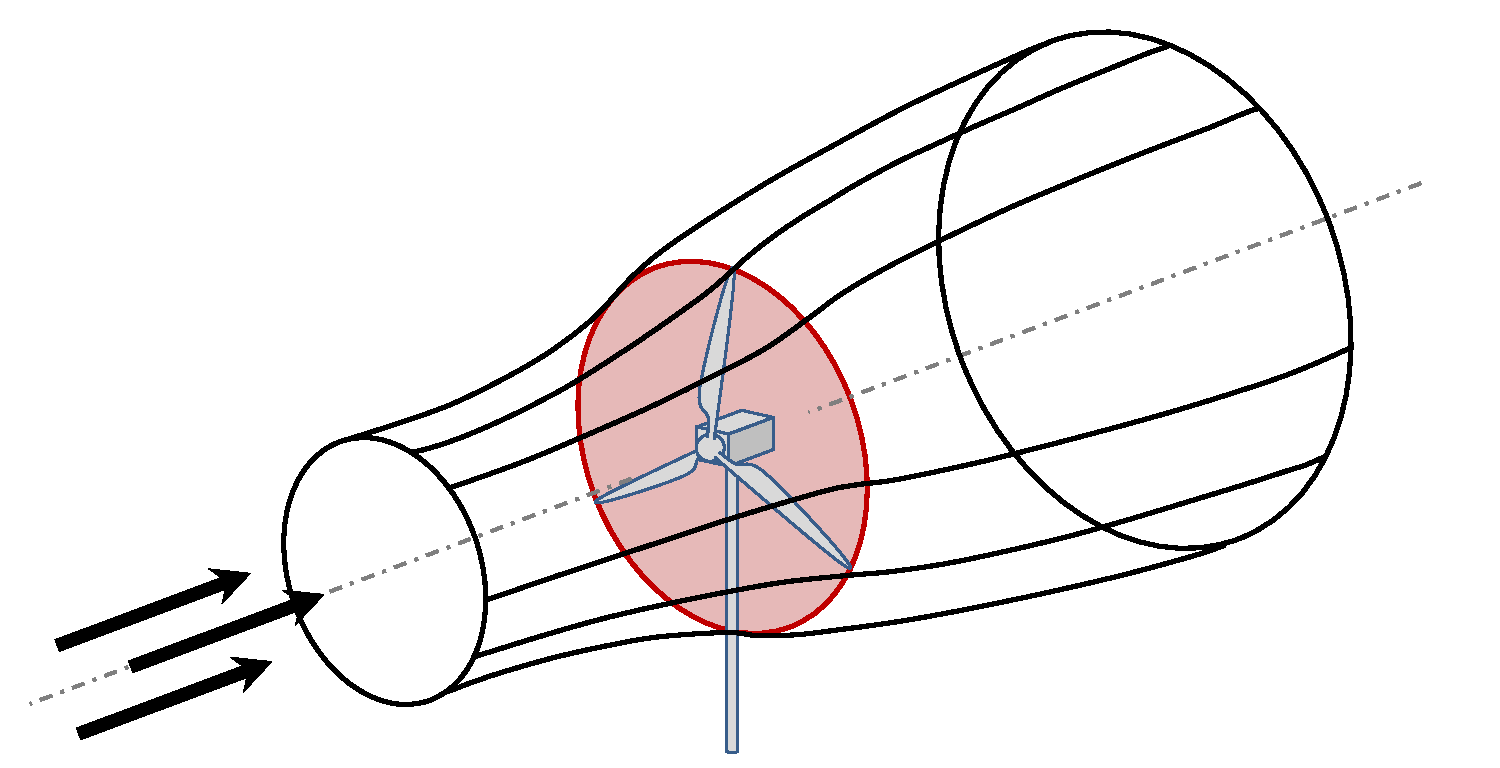
\includegraphics[scale=0.5]{\EPSDIR/Wind_Turbine_fig/Tube.pdf}
\caption{Stream-tube around the rotor disk of a wind turbine. \citet{joulin2019modelisation} adapted from \citet{burton2001wind}}  
\label{fig:BEMTube3D}
\end{figure}		
		
\medbreak
A vertical cut of the stream-tube is given in Figure \ref{fig:BEMTubeEq}. One can write $U$ the axial velocity, $p$ the pressure and $A$ the cross-sectional area. The indices $_\infty$, $_d$ and $_W$ indicate respectively the upstream, disk and downstream positions. The exponents $^+$ and $^-$ indicate the infinitesimal upstream and downstream sides of the disc. The thrust force $F_T$ writes:
\begin{equation}
\label{eq:FpDef}
F_T = A_d (p_d^+ - p_d^-).
\end{equation}		
\medbreak
\begin{figure}[h]
\centering
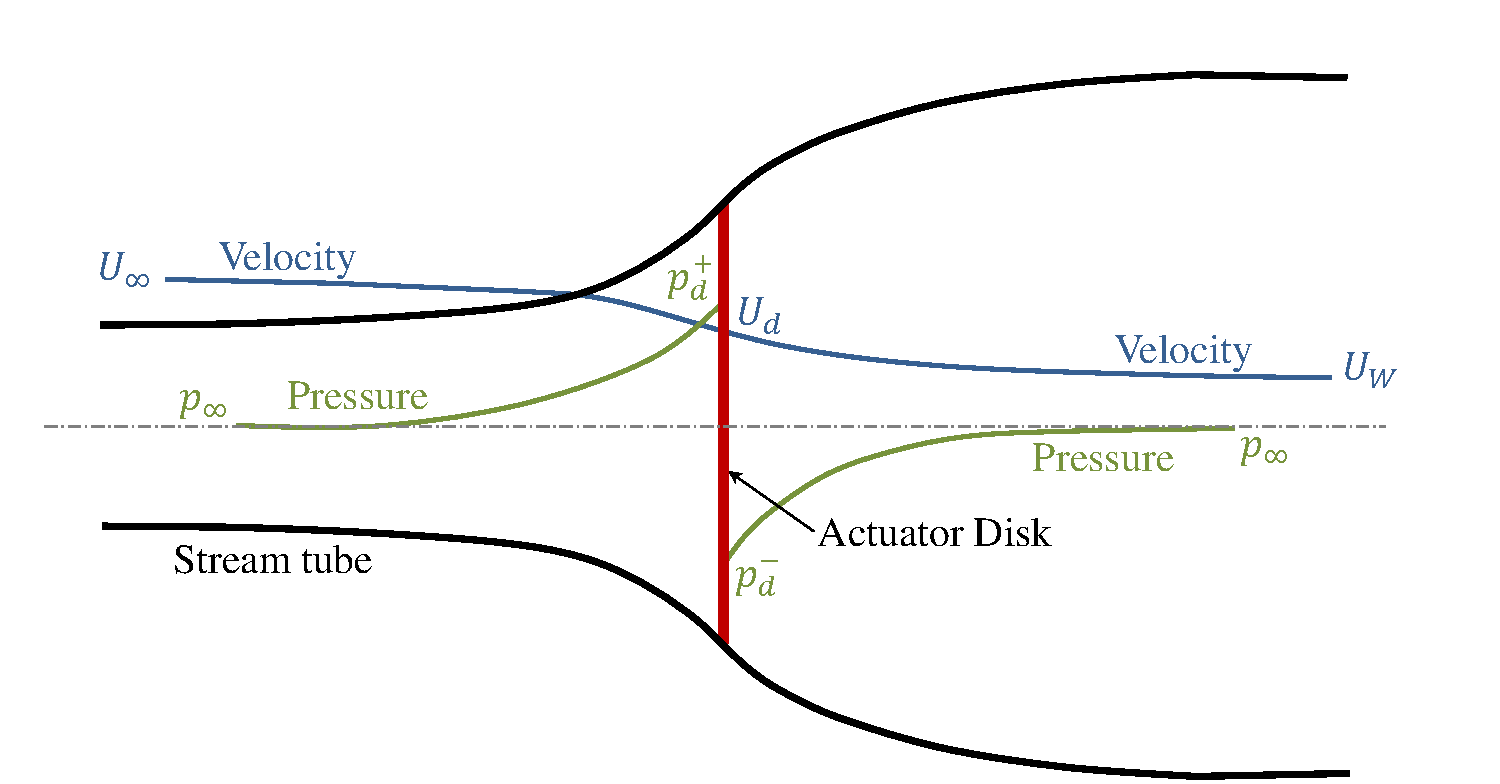
\includegraphics[scale=0.5]{\EPSDIR/Wind_Turbine_fig/Tube_Eq.pdf}
\caption{Vertical cut of the stream-tube around the rotor disk of a wind turbine and its variables. \citet{joulin2019modelisation} adapted from \citet{burton2001wind}}  
\label{fig:BEMTubeEq}
\end{figure}
\medbreak
	
It is possible to apply the Bernoulli’s theorem to the upstream part, and to the downstream one, separately. It gives: 
\begin{equation}
\label{eq:Bern}
\left\lbrace
\begin{array}{ccc}		
p_\infty + \dfrac{1}{2} \rho U_\infty^2 = p_d^+ + \dfrac{1}{2} \rho U_d^2
\\
p_d^- + \dfrac{1}{2} \rho U_d^2 = p_\infty+ + \dfrac{1}{2} \rho U_W^2,
\\
\end{array}\right.
\end{equation}
where $\rho$ is the air density. Using (\ref{eq:Bern}) in (\ref{eq:FpDef}), the thrust force becomes:
\begin{equation}
\fbox{$
F_T = \dfrac{1}{2} \rho A_d (U_\infty^2 -  U_W^2)
$}.
\label{eq:FpBern}
\end{equation}		

This first expression gives the thrust force by knowing the upstream velocity: $F_T = f(U_\infty)$. In practice, it is impossible to define a proper $U_\infty$. Then, an expression with the velocity at the disk position: $F_T = f(U_d)$ has to be found. It is the aim of the next paragraphs.



		\subsubsection*{Momentum theory}
				\label{p:ADNRAppliTheo}
The axial induction factor $a$ describes the percentage of velocity deficit:
\begin{equation}
U_d = U_\infty( 1 - a ).
\label{eq:a}
\end{equation}
By applying the moment theory, the thrust force $F_T$ can be expressed at the position of the disc (see \citet{joulin2019modelisation} for more details) as:
\begin{equation}	
\label{eq:FpD}	
\fbox{$
F_T = \dfrac{1}{2} \rho A_d U_d^2 \dfrac{4a}{1-a}.
$}			
\end{equation}

The thrust coefficient $C_{T_\infty}$ is the rate between the thrust force and the dynamic force of the wind. One can note that it is defined with the upstream velocity $U_\infty$. It can be expressed using the axial induction factor $a$:
\begin{equation}	
\label{eq:ct}	
C_{T_\infty} = \dfrac{F_T}{\dfrac{1}{2} \rho A_d U_\infty^2} = 4 a (1 -a).
\end{equation}	

		\subsubsection*{Final expression of thrust force}

The thrust coefficient $C_{T_\infty}$  is a well-known data (tabulated data $C_{T_\infty} = f(U_{\infty})$ given by the constructor). Then, by using  (\ref{eq:ct}), one can write $a$ as:
\begin{equation}
a = \dfrac{1}{2}(1-\sqrt{1-C_{T_\infty}}).
\end{equation}
Then, one can define $C_{T_d}$:
\begin{equation}	
C_{T_d} = \dfrac{4a}{1 -a},
\end{equation}	
to finally obtain a suitable expression for the thrust coefficient, using $U_d$ only:
\begin{equation}
\fbox{$
F_T = \dfrac{1}{2} \rho A_d U_d^2 C_{T_d}
$}.
\label{eq:finadnr}
\end{equation}  

%++++++++++++++++++++++++++++++++
\subsection{Numerical implementation}
%++++++++++++++++++++++++++++++++

In Meso-NH, the ADNR is discretised according to the mesh, as illustrated in Fig. \ref{fig:adnum}.
\begin{figure}[h]
\centering
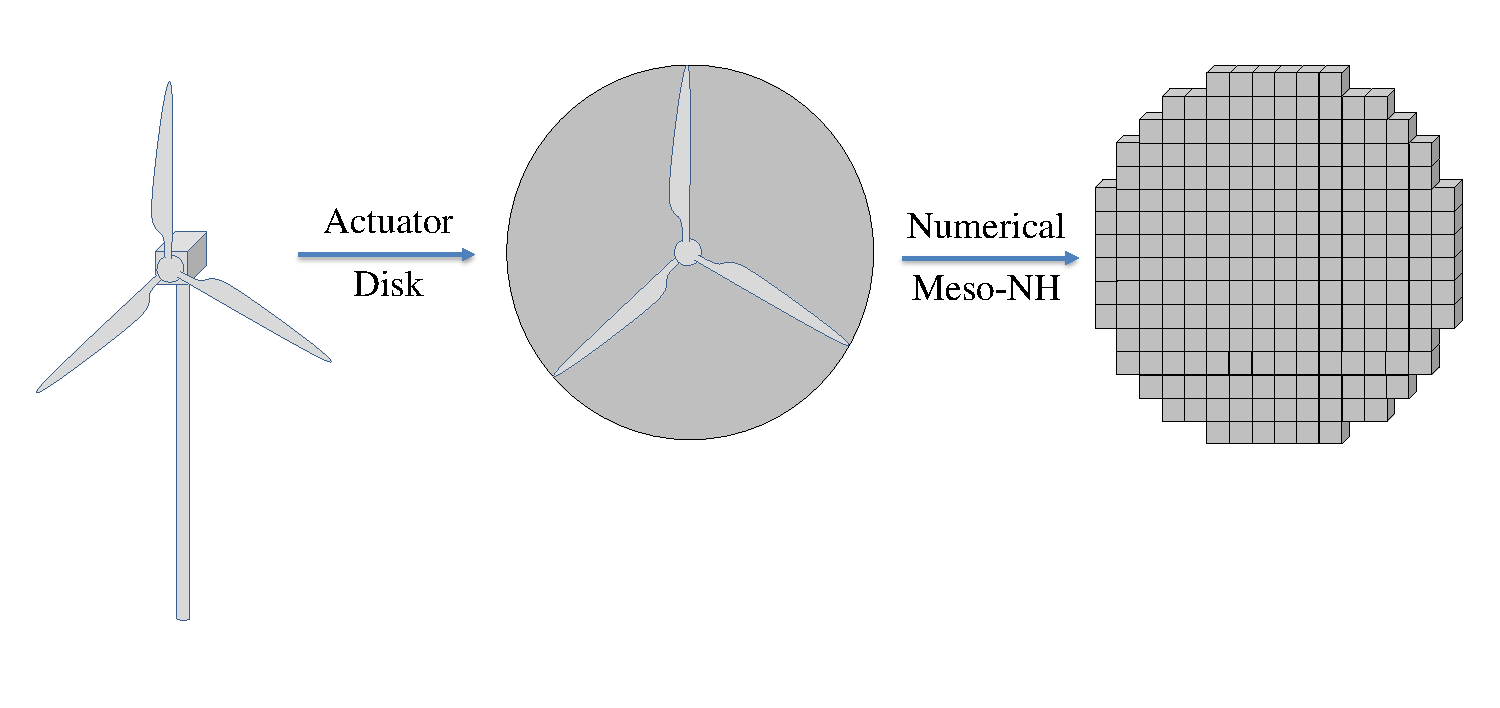
\includegraphics[scale=0.5]{\EPSDIR/Wind_Turbine_fig/ADnum.pdf}
\caption{Discretization of the ADNR \citet{joulin2019modelisation}.}
\label{fig:adnum}  
\end{figure}
\medbreak
The first step of the coupling algorithm is to find the cells where the infinitesimal thrust forces will be applied. It is done by checking if the cell is located into the rotor disk. Then, the wind speed of the cell $U_d$ is extracted, after it has been evaluated at mass point (C-type of Arakawa). It is possible to use the closest value of the wind, or to interpolate it from the 8-neighborhood cells. Finally, the discrete thrust force is calculated by using (\ref{eq:finadnr}) as follows:
\begin{equation}
\fbox{$
dF_T = \dfrac{1}{2} \rho \Delta y \Delta z U_d^2 C_{T_d}
$},
\label{eq:adnrft}
\end{equation}
where $\Delta y \Delta z$ is the vertical area of the cell. This force will act against the wind field, as shown in Figure \ref{fig:appluforceadnr}. This is why, in the end, the force $dF_{T_{WT\rightarrow WIND}} = -dF_T$ is added to the global momentum budget of Meso-NH. 
\begin{figure}[h]
\centering
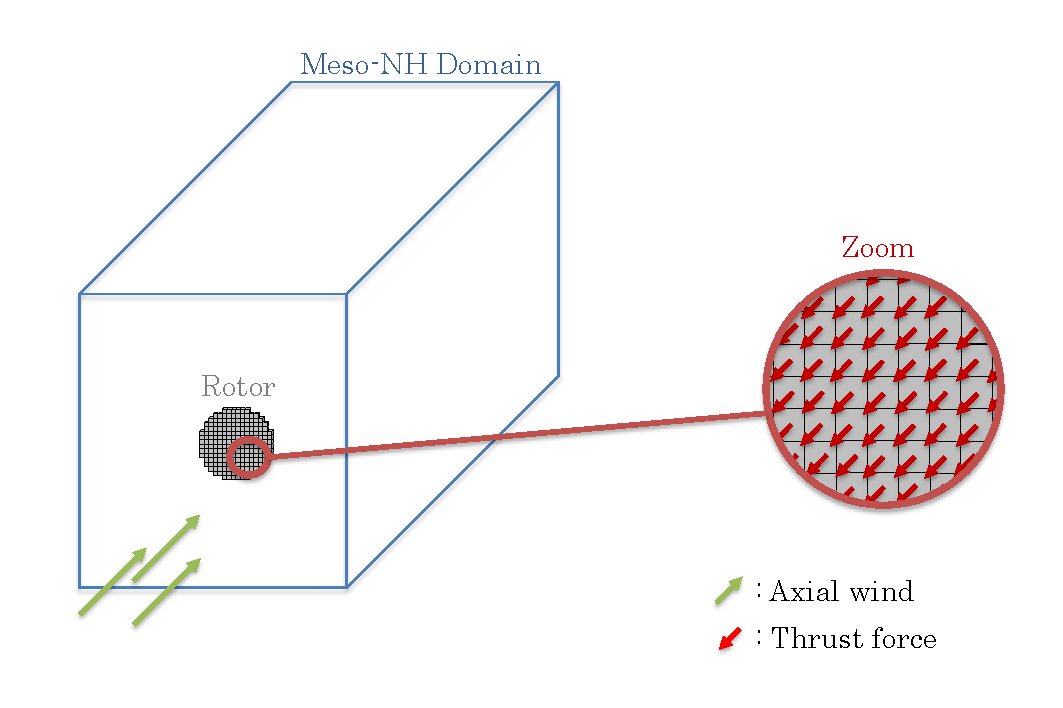
\includegraphics[scale=0.6]{\EPSDIR/Wind_Turbine_fig/ApplyForceADNR.pdf}
\caption{Applying discrete thrust forces in Meso-NH \citet{joulin2019modelisation}.}
\label{fig:appluforceadnr}  
\end{figure}

%++++++++++++++++++++++++++++++++
\subsection{Additional implementations}
%++++++++++++++++++++++++++++++++		
\subsubsection*{1D Linear smearing}
\label{sss:1dsmearADNR}
To avoid numerical instabilities, it is possible to apply a linear smearing to the force field. It is done by using the C-type cells of Arakawa. To smear the forces linearly, one can apply successively:
\begin{equation}
dF_{x_{i}^m} = \dfrac{dF_{x_{i}^f} + dF_{x_{i+1}^f}}{2},
\end{equation}
and then,
\begin{equation}
dF_{x_{i}^f} = \dfrac{dF_{x_{i}^m} + dF_{x_{i+1}^m}}{2},
\end{equation}
where $x_i^m$ and $x_i^f$ are respectively  the mass point and the flux point of the $i^{th}$ cell of $x$-axis. An illustration is given in Figure \ref{fig:smearinglin}. This method is less expensive numerically than the usual convolution product, and seems to provide similar results. See \citet{joulin2019modelisation} for discussions.

\begin{figure}[h]
\centering
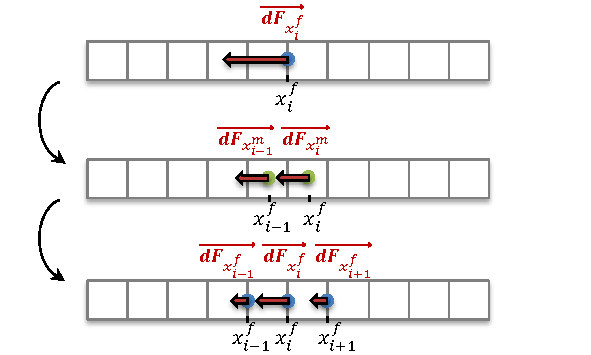
\includegraphics[scale=1]{\EPSDIR/Wind_Turbine_fig/Smearing_Linear.pdf}
\caption{Scheme of an 1D linear smearing of the force field \citet{joulin2019modelisation}.}
\label{fig:smearinglin}  
\end{figure}

\subsubsection*{3D linear smearing}
\label{sss:3dsmearADNR}
It is possible to use a 3D linear smearing based on the 1D Linear distribution, by applying the same method on $y$-axis and $z$-axis successively.


%%%%%%%%%%%%%%%%%%%%%%%%%%%%%%%
\section{Rotating Actuator Disk (ADR)}
%%%%%%%%%%%%%%%%%%%%%%%%%%%%%%%

%++++++++++++++++++++++++++++++++
\subsection{Overview}
%++++++++++++++++++++++++++++++++
In the Actuator Disk model developed by \citet{rankine1865mechanical} and \citet{froude1889part}, rotor rotation and tangential forces are neglected. The Rotating Actuator Disk (ADR) model addresses these effects by incorporating the Blade Element (BE) theory developed by \citet{glauert1935airplane}. This theory involves dividing the blade into multiple sections and studying the flow over each section (Figure \ref{fig:Decoupage2D}). It is used to assess the forces acting on a blade based on the lift and drag forces generated at each section of the blade.

\begin{figure}[h]
\centering
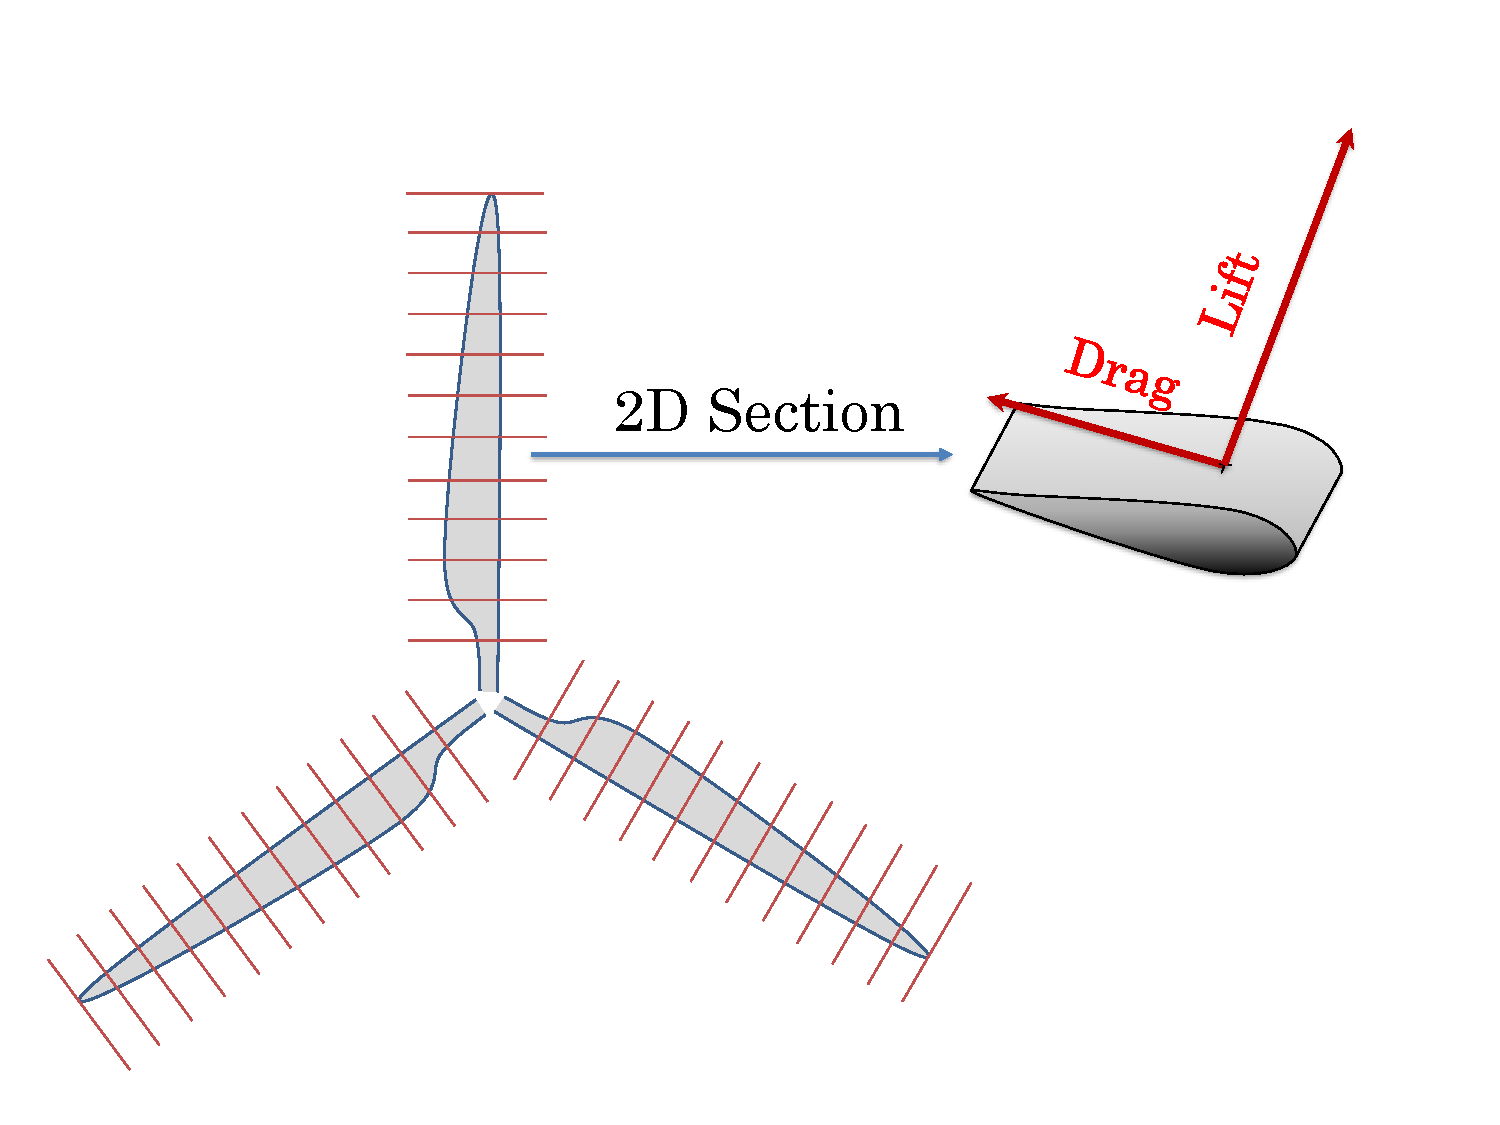
\includegraphics[scale=0.4]{\EPSDIR/Wind_Turbine_fig/Decoupage2D.pdf}
\caption{Schematic representation of Blade Element theory \citet{joulin2019modelisation}.}
\label{fig:Decoupage2D}
\end{figure}
\medbreak
Based on the principle of `body forces', the ADR method does not explicitly represent the geometry of the blades. Once again, the rotor effect is considered through equivalent volume forces. With the ADR, not only is the thrust force of the turbine on the wind modeled, but also the rotor torque, which is not considered in the ADNR model. The concept involves considering an average effect of the blades on the surface they sweep during their rotations. In this methodology, the ADR is discretized in a cylindrical coordinate system, with a certain number of azimuthal elements (segmented by $\Delta \theta$) and radial elements (segmented by $dr$), as shown in Figure \ref{fig:ADR_mesh}. At each time step and at a specific radial location $r$, each azimuthal position carries the effects of the blades, weighted by the ratio of the surface element to the total annular surface at the given $r$.

\begin{figure}[h]
\centering
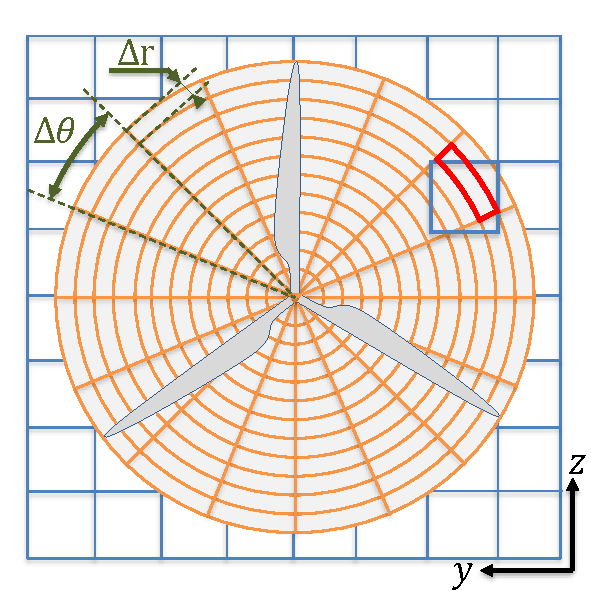
\includegraphics[scale=0.8]{\EPSDIR/Wind_Turbine_fig/ADR_mesh.pdf}
\caption{Overview of ADR mesh \citet{joulin2019modelisation}.}
\label{fig:ADR_mesh}
\end{figure}
\medbreak

To enhance the representation of wind wakes, \citet{sorensen1992unsteady} introduced the rotation of the Actuator Disk model in their CFD code. Their work demonstrates that this addition provides fundamental insights into wake characteristics (\citet{sorensen1995model, sorensen1998analysis}). Subsequent studies by \citet{madsen1997cfd} and \citet{mikkelsen2003actuator} focused on wind turbines with pre-cones or misalignment to the wind direction.

Later on, the ADR wind turbine model was coupled with Large Eddy Simulation (LES) by the EPFL team (\citet{porte2011large, wu2011large, wu2015modeling, porte2014interaction}). This coupling enables a simple yet effective representation of the wind turbine while leveraging the detailed turbulence representation provided by LES. This approach allowed the study of wake evolution and its impacts on the atmospheric boundary layer.

Subsequently, ADR was coupled with WRF LES, a U.S. atmospheric code, to initiate the study of real wind farms (\citet{aitken2014utility, aitken2014large, mirocha2014implementation, mirocha2015investigating, marjanovic2015simulation}). These studies aimed to analyze wind farm layout and wake evolution, with the ultimate goal of optimizing wind resource exploitation, potentially through control and command strategies.


%++++++++++++++++++++++++++++++++
\subsection{Theory}
%++++++++++++++++++++++++++++++++
\subsubsection*{Hypotheses}
\label{ss:hypADR}
The model is based on a number of assumptions:
\begin{itemize}
\item Incompressible flow,
\item 2D flow along the airfoils,
\item No aerodynamic interaction between each blade element (which excludes any radial flow),
\item As the wind turbine is simplified to a porous disk, an infinite number of blades is considered.
\end{itemize}

\subsubsection*{Wind turbine kinematics and frames}		
\label{ss:EOL_M_cinematiqueADR}
The wind turbine can be divided into different kinematic classes. As shown in Figure \ref{fig:ADR_frames}, each class has its own frame:
\begin{multicols}{2}
\begin{itemize}
\item the domain associated with $R_G$ frame,
\item the tower associated with $R_T$ frame,
\item the nacelle associated with $R_N$ frame,
\item the hub associated with $R_H$ frame.
\end{itemize}
\end{multicols}
In this implementation, the rotation of the wind turbine is taken into account by applying the rotational movement of the hub frame around the nacelle frame. To ease computations, 2 other frames have been created:
\begin{itemize}
\item the cylindrical frame $R_{C}$, linked to the hub frame,
\item frames attached to discretized annular elements: the $j^{th}$ radial elements of the $i^{th}$ azimutal element $R_{E_{ij}}$ frames.
\end{itemize}
\medbreak
The rotation matrices $\mathcal{M}_{R_\clubsuit \rightarrow R_\spadesuit}$ are determined at each time step to move from a frame to another one. The kinematic relations allow to know the translational and rotational velocities of each blade element. Details about these relations can be found in \citet{joulin2019modelisation}, \textit{Annexe C} (applied to Actuator Line).
\medbreak

\begin{figure}
    \centering
    \begin{minipage}{0.32\textwidth}
        \centering
        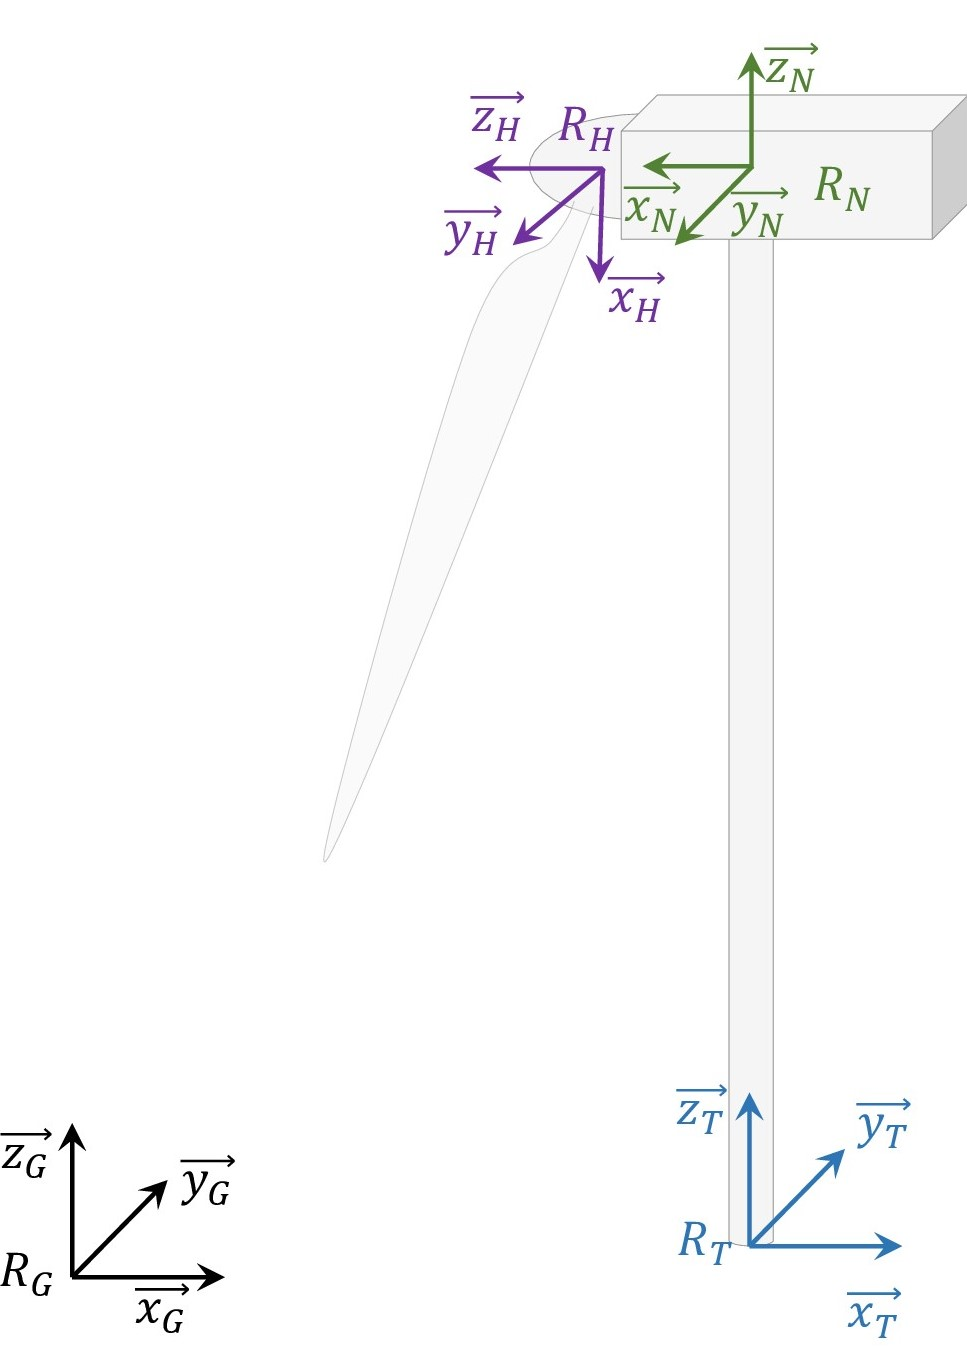
\includegraphics[width=\textwidth]{\EPSDIR/Wind_Turbine_fig/RepereADR_Gen.jpg}
        %\subcaption{}
        \label{fig:a}
    \end{minipage}
    \hfill
    \begin{minipage}{0.32\textwidth}
        \centering
        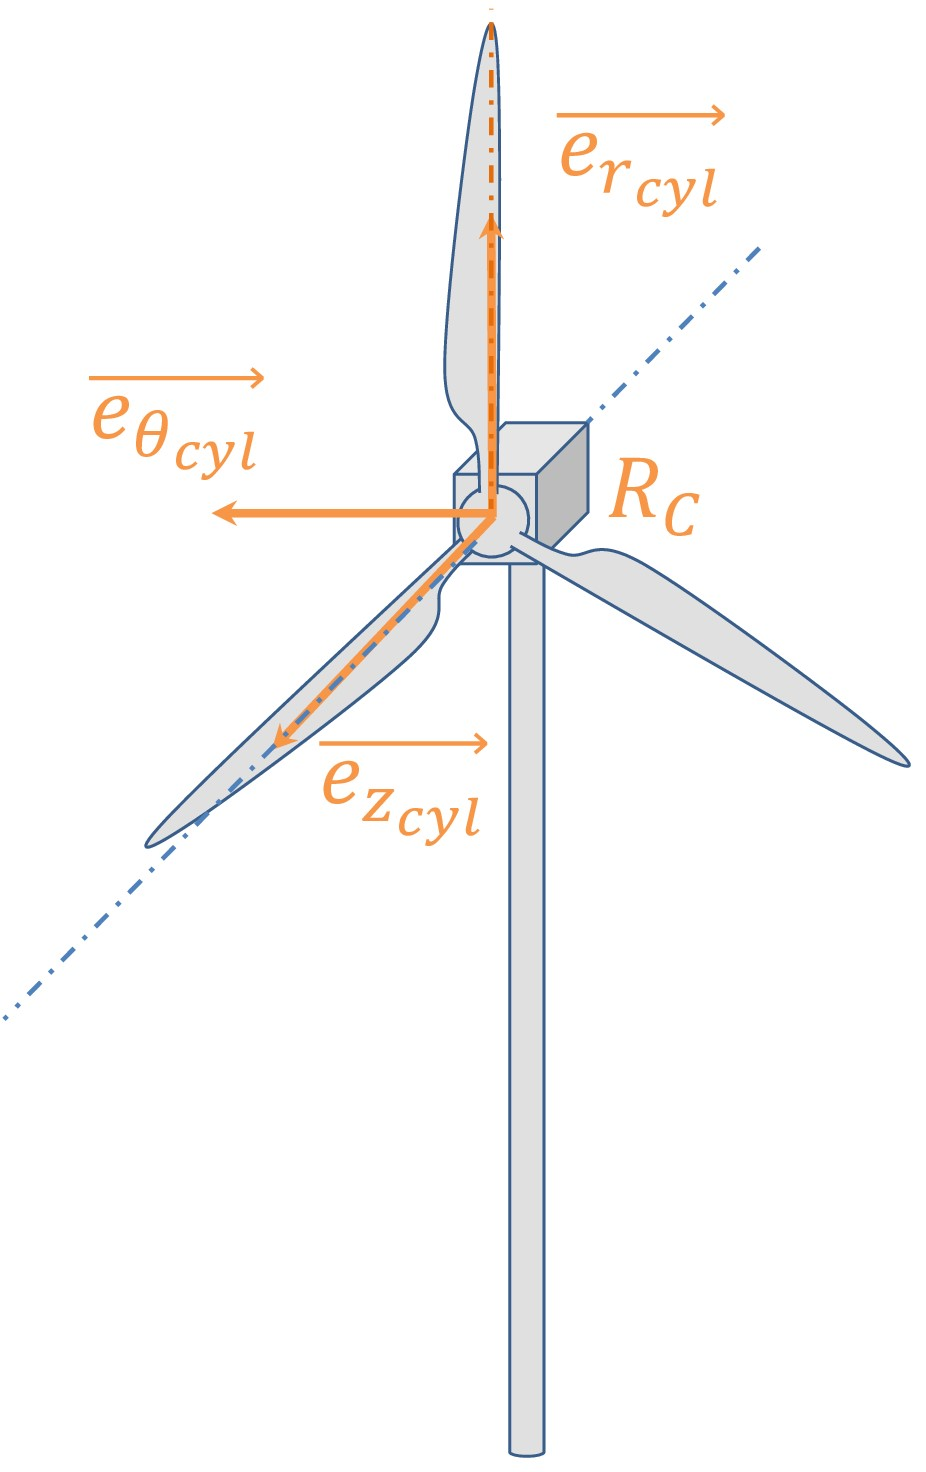
\includegraphics[width=0.8\textwidth]{\EPSDIR/Wind_Turbine_fig/RepereADR_Cyl.jpg}
        %\subcaption{}
        \label{fig:b}
    \end{minipage}
    \hfill
    \begin{minipage}{0.32\textwidth}
        \centering
        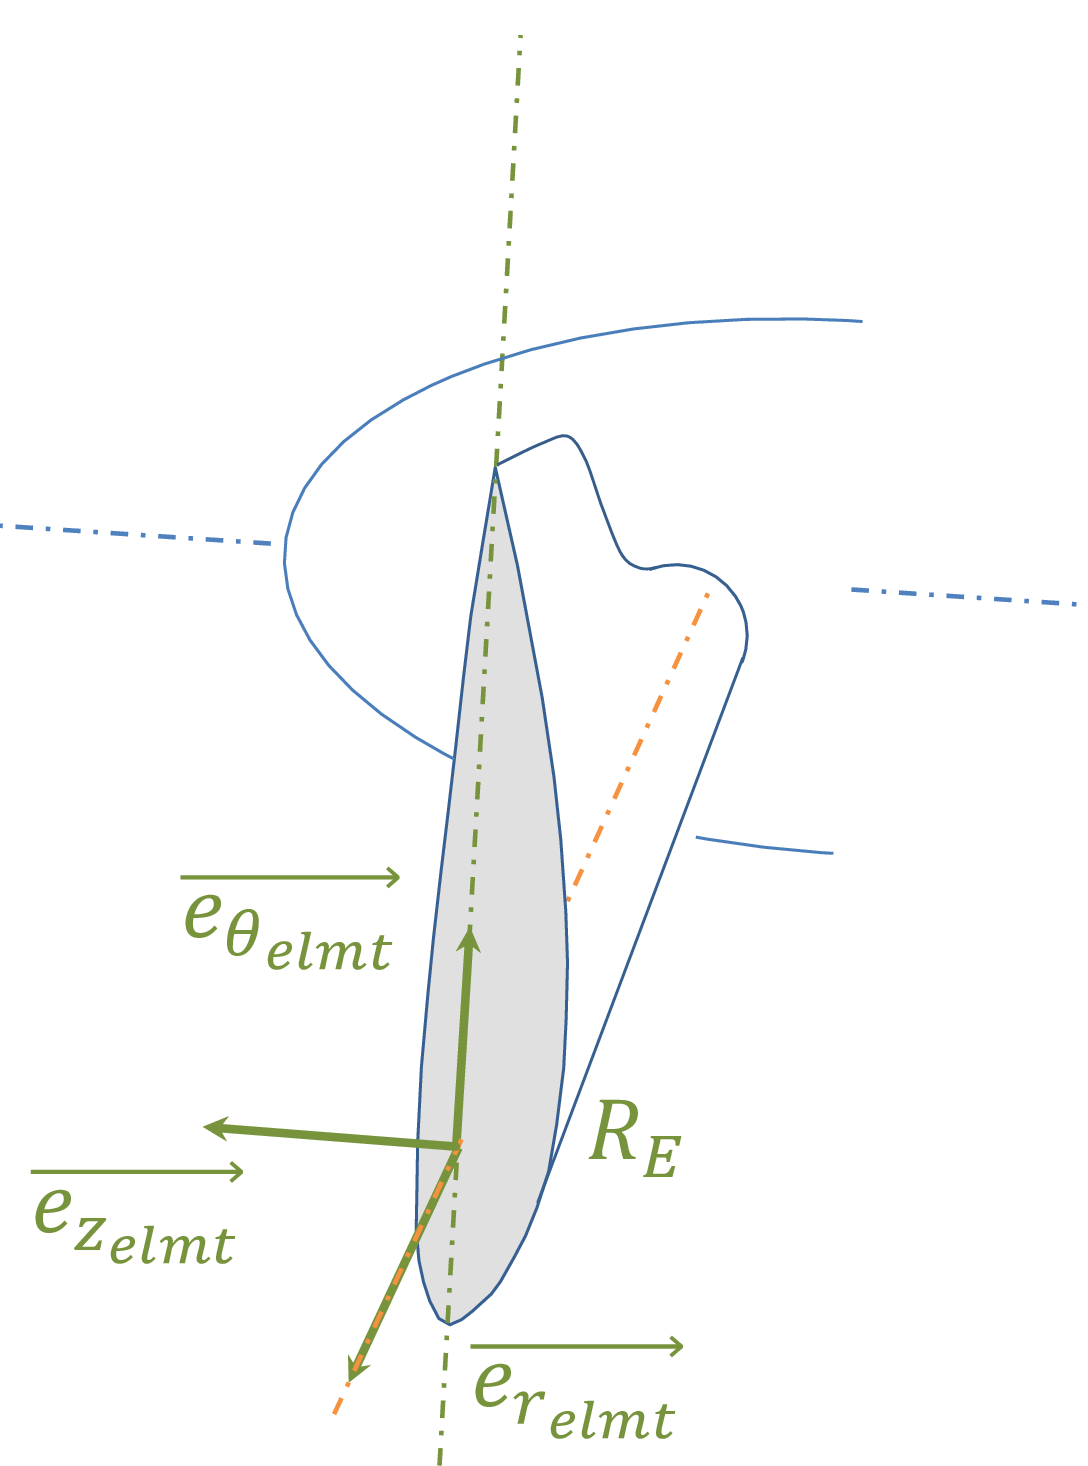
\includegraphics[width=\textwidth]{\EPSDIR/Wind_Turbine_fig/RepereADR_Elmt.png}
        %\subcaption{}
        \label{fig:c}
    \end{minipage}
    \caption{Illustration of ADR's frames. Left: global, tower, nacelle, and hub frames. Middle: cylindrical frame. Right: element frame.}
    \label{fig:ADR_frames}
\end{figure}

\subsubsection*{Applying blade element theory}

\paragraph*{Determination of $U_{rel}$ and $\alpha$:}
Thanks to the kinematic definition and to the rotation matrices, the determination of the relative wind $U_{rel}$ is almost direct. Indeed, the kinematic relations enable to know the velocity of translation $U^{ij}_{trans}$. Considering the $j^{th}$ elements of the $i^{th}$ blade located in a surrounding volume of air with a velocity $U^{ij}_{wind}$, the relative velocity writes:
\begin{equation}
\label{eq:ADR_urel}
\fbox{$
\overrightarrow{U^{ij}_{rel}}_{\vert _{R_{E_{ij}}}} = \mathcal{M}_{R_{E_{ij}} \rightarrow R_{G_{ij}}} \times \overrightarrow{U^{ij}_{wind}}_{\vert _{R_{G_{ij}}}} - \overrightarrow{U^{ij}_{trans}}_{\vert _{R_{E_{ij}}}}
$}.
\end{equation}
And the angle of attack $\alpha$ can be evaluated thanks to:
\begin{equation}
\label{eq:ADR_alpha}
\fbox{$
\alpha = tan^{-1} \left( \dfrac{\overrightarrow{U^{ij}_{rel}}_{\vert _{R_{E_{ij}}}} \cdot \overrightarrow{x}}{\overrightarrow{U^{ij}_{rel}}_{\vert _{R_{E_{ij}}}} \cdot \overrightarrow{y}} \right)
$}.
\end{equation}

\paragraph*{Aerodynamic forces:}
By knowing $U_{rel}$ and $\alpha$, the blade element theory can be applied. The aerodynamic forces can be expressed in the aerodynamic frame as:
\begin{equation}
\label{eq:eol_m_adr_eff}	
\left\lbrace
\begin{array}{ccc}	
dF_{L} = \dfrac{1}{2} \rho S U_{rel}^2 C_L(\alpha),
\\   
\\
dF_{D} = \dfrac{1}{2} \rho S U_{rel}^2 C_D(\alpha).
\\
\end{array}\right.
\end{equation}	

where the lift $C_L$ and drag $C_D$ coefficients are known according to the angle of attack $\alpha$ and the Reynolds number $Re$. The lifting surface $S$, evaluated with the airfoil chord $c$ and the radial width $dr$ ($S = c dr$).
\medbreak
This elementary force represents the force from a section of one blade (not from an annular element). Applying this force throughout the infinite number of blades would be incorrect. To ensure momentum conservation, the loads need to be distributed evenly over the discretized disc. This is achieved using the ratio between the number of blades $N_{\text{blades}}$ and the number of azimuthal elements $2\pi/\Delta\theta$. Introducing a new surface $S'$ defined as:
\begin{equation}
S' = S N_{blades} \dfrac{\Delta\theta}{2\pi},
\end{equation}
One can obtain:
\begin{equation}
\label{eq:eol_m_adr_final}        
\fbox{$
\left\lbrace
\begin{array}{ccc}      
df_{L} = \dfrac{1}{2} \rho S' U_{rel}^2 C_L,
\\   
\\
df_{D} = \dfrac{1}{2} \rho S' U_{rel}^2 C_D.
\\
\end{array}\right.
$}
\end{equation}
By applying a rotation angle $a$, the forces can be expressed in $R_{E_{ij}}$, and then in the global frame by using $\mathcal{M}_{R_{G_{ij}} \rightarrow R_{E_{ij}}}$.


%++++++++++++++++++++++++++++++++
\subsection{Numerical implementation}
%++++++++++++++++++++++++++++++++

The first step of the Rotating Actuator Disc is to compute the kinematics of the wind turbine. The kinematic algorithm computes, at each time step, the new positions and velocities of all elements. 
Knowing the position of an annular blade element, the local wind speed can be extracted. To do so, the wind speed is computed at mass point. Then, it is possible to use the closest value (from the blade element) of the wind, or to interpolate it from the 8-neighborhood cells.
Afterwards, the relative velocity is computed using (\ref{eq:ADR_urel}), and the angle of attack $\alpha$ with (\ref{eq:ADR_alpha}). The aerodynamic coefficients $C_L$ and $C_D$ are then computed by knowing $\alpha$, from a spline-cubic interpolation of the tabulated input data. Finally, the aerodynamic forces are computed in the aerodynamic frame using (\ref{eq:eol_m_adr_final}): 
\begin{equation}
\label{eq:eol_m_alm_eff_num}	
\fbox{$
\left\lbrace
\begin{array}{ccc}	
df_{L} = \dfrac{1}{2} \rho S' U_{rel}^2 C_L(\alpha),
\\   
\\
df_{D} = \dfrac{1}{2} \rho S' U_{rel}^2 C_D(\alpha).
\\
\end{array}\right.
$}
\end{equation}	
A last change of frame enables the projection of these forces to the global momentum budget of Meso-NH. One can note that, for the moment, only the effects of the blades are computed: the nacelle and the tower are neglected. 

Note: Special attention must be given to the number of radial (NNB\_RADELT) and azimuthal (NNB\_AZIELT) elements depending on the mesh used in Meso-NH. To avoid gaps in the mesh and ensure a proper distribution of efforts, it is recommended to have:
\begin{equation}
NNB\_RADELT > \dfrac{2R}{\min(\Delta x, \Delta y, \Delta z)}
\end{equation}
and
\begin{equation}
NNB\_AZIELT > \pi / \sin^{-1} \left( \dfrac{\min(\Delta x, \Delta y, \Delta z)}{2R} \right)
\end{equation}
where $R$ is the radius of the rotor, and $\min(\Delta x, \Delta y, \Delta z)$ is the smallest dimension of the Meso-NH mesh at the rotor level.

%++++++++++++++++++++++++++++++++
\subsection{Additional implementations}
%++++++++++++++++++++++++++++++++
\subsubsection*{1D linear smearing}
It is possible to use the 1D linear smearing mentionned in \ref{sss:1dsmearADNR}.

\subsubsection*{3D linear smearing}
It is possible to use the 3D linear smearing mentionned in \ref{sss:3dsmearADNR}.

\subsubsection*{Tip loss correction}
\label{sss:tiplossADR}
As an infinite number of blades is considered in this Actuator method, the induction of each blade is not well reproduced, and the tip vortices are not properly modeled. To overcome this issue, \citet{glauert1935airplane} developed the so-called tip loss correction. It introduces a factor $F$ to take into account the wake-induced losses:
\begin{equation}
F = \dfrac{2}{\pi} \arccos( e^{-f})
\end{equation}
where $f$ can be expressed using the radius of the tip $r_{tip}$ and the flow angle $\varphi$:
\begin{equation}
f=
\dfrac{N_{pales}}{2} \dfrac{r_{tip}-r}{r sin(\varphi)}
\end{equation}
Then, the factor is introduced as follows:
\begin{equation}	
\label{eq:ADR_tiploss}
\left\lbrace
\begin{array}{ccc}	
dF_{L} = \dfrac{1}{2} C_L \rho S' U_{rel}^2 F,
\\   
\\
dF_{D} = \dfrac{1}{2} C_D \rho S' U_{rel}^2 F.
\\
\end{array}\right.
\end{equation}	

%%%%%%%%%%%%%%%%%%%%%%%%%%%%%%%
\section{Actuator Line Method (ALM)}
%%%%%%%%%%%%%%%%%%%%%%%%%%%%%%%
%++++++++++++++++++++++++++++++++
\subsection{Overview}
%++++++++++++++++++++++++++++++++

The previous model, the ADR, can be seen as the average of the blade motion over one or several rotations. It gives the tendency of the wake, but it cannot represent its instantaneous particularities. To overcome this problem, it is possible to use lines to model the blades, instead of a disk: it is the \textit{Actuator Line Method} (ALM). The method has been generalized by \citet{sorensen2002numerical}. Each blade applies a force on the fluid, as shown in Figure \ref{fig:AL_principe}. In order to find the position of the blades and their velocity, it is necessary to take into account their kinematic motion. Then, the blade element theory allows to determine the aerodynamic forces to apply.

\begin{figure}[h]
\centering
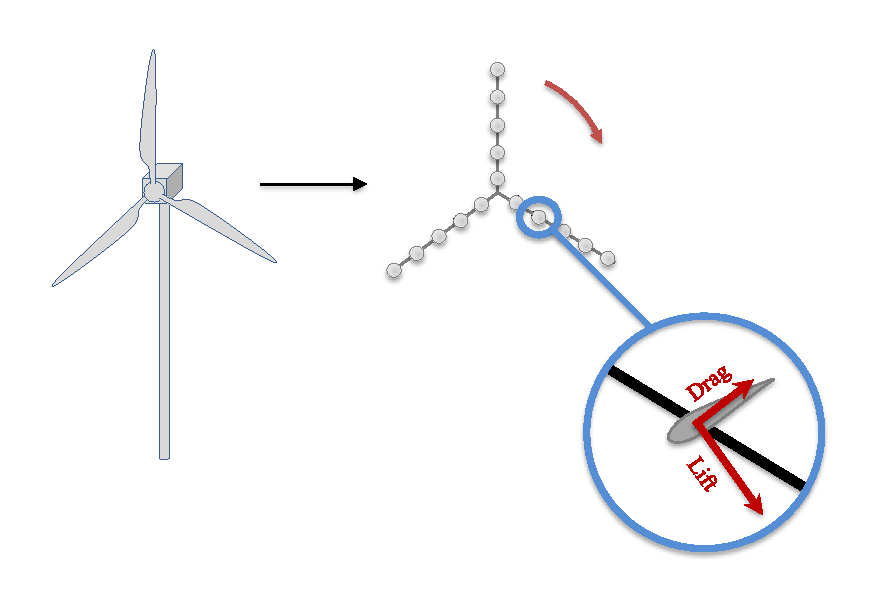
\includegraphics[scale=1]{\EPSDIR/Wind_Turbine_fig/ALprincipe.pdf}
\caption{Overview of the Actuator Line Method \citet{joulin2019modelisation}.}  
\label{fig:AL_principe}
\end{figure}
\medbreak
The first coupling between the Actuator Line Method and a CFD code has been introduced by \citet{mikkelsen2003actuator}. It allows to reproduce the helical shape of the unsteady wake and capturing tip and root vortices (\citet{ivanell2007numerical}, \citet{ivanell2007numericalv}) giving a better description of the wake downstream the wind turbines (\citet{Ivanell2009}, \citet{Troldborg2009}).
\medbreak
For these reasons, the ALM has been introduced in several LES frameworks (\citet{porte2011large} or \citet{tabib2017near}). Interactions between wind turbines and atmospheric boundary layer have been studied (\citet{lu2011large}, \citet{lu2015impact}). It has also been coupled with WRF-LES (\citet{marjanovic2015simulation} and \citet{marjanovic2017implementation}) for wind farm studies, or in SOWFA, based on OpenFOAM  \citet{Churchfield2012}. The coupling with Meso-NH has been introduced by \citet{joulin2020theactuator}.


%++++++++++++++++++++++++++++++++
\subsection{Theory}
%++++++++++++++++++++++++++++++++
\subsubsection*{Hypotheses}
\label{ss:hypALM}
The model is based on a number of assumptions:
\begin{itemize}
\item Incompressible flow,
\item 2D flow along the airfoils,
\item No aerodynamic interaction between each blade element (which excludes any radial flow).
\end{itemize}
\subsubsection*{Wind turbine kinematics and frames}		
\label{ss:EOL_M_cinematiqueAL}

The wind turbine can be divided into different kinematic classes. As shown in Figure \ref{fig:ALrep}, each class has its own frame:
\begin{multicols}{2}
\begin{itemize}
\item the domain associated with $R_G$ frame,
\item the tower associated with $R_T$ frame,
\item the nacelle associated with $R_N$ frame,
\item the hub associated with $R_H$ frame,
\item the $i^{th}$ blade associated with $R_{B_i}$ frames,
\item the $j^{th}$ elements of the $i^{th}$ blade associated with $R_{E_{ij}}$ frames.
\end{itemize}
\end{multicols}
\medbreak
Even if there is no motion between the blade elements and their blade, the frames $R_{E_{ij}}$ linked to the sections have been introduced to make the aerodynamic calculations easier. The rotation matrices $\mathcal{M}_{R_\clubsuit \rightarrow R_\spadesuit}$ are determined at each time step to move from a frame to another one. The kinematic relations allow to know the translational and rotational velocities of each blade element. Details about these relations can be found in \citet{joulin2019modelisation}, \textit{Annexe C}.
\medbreak
\begin{figure}[h]
\hspace{-1.8cm}
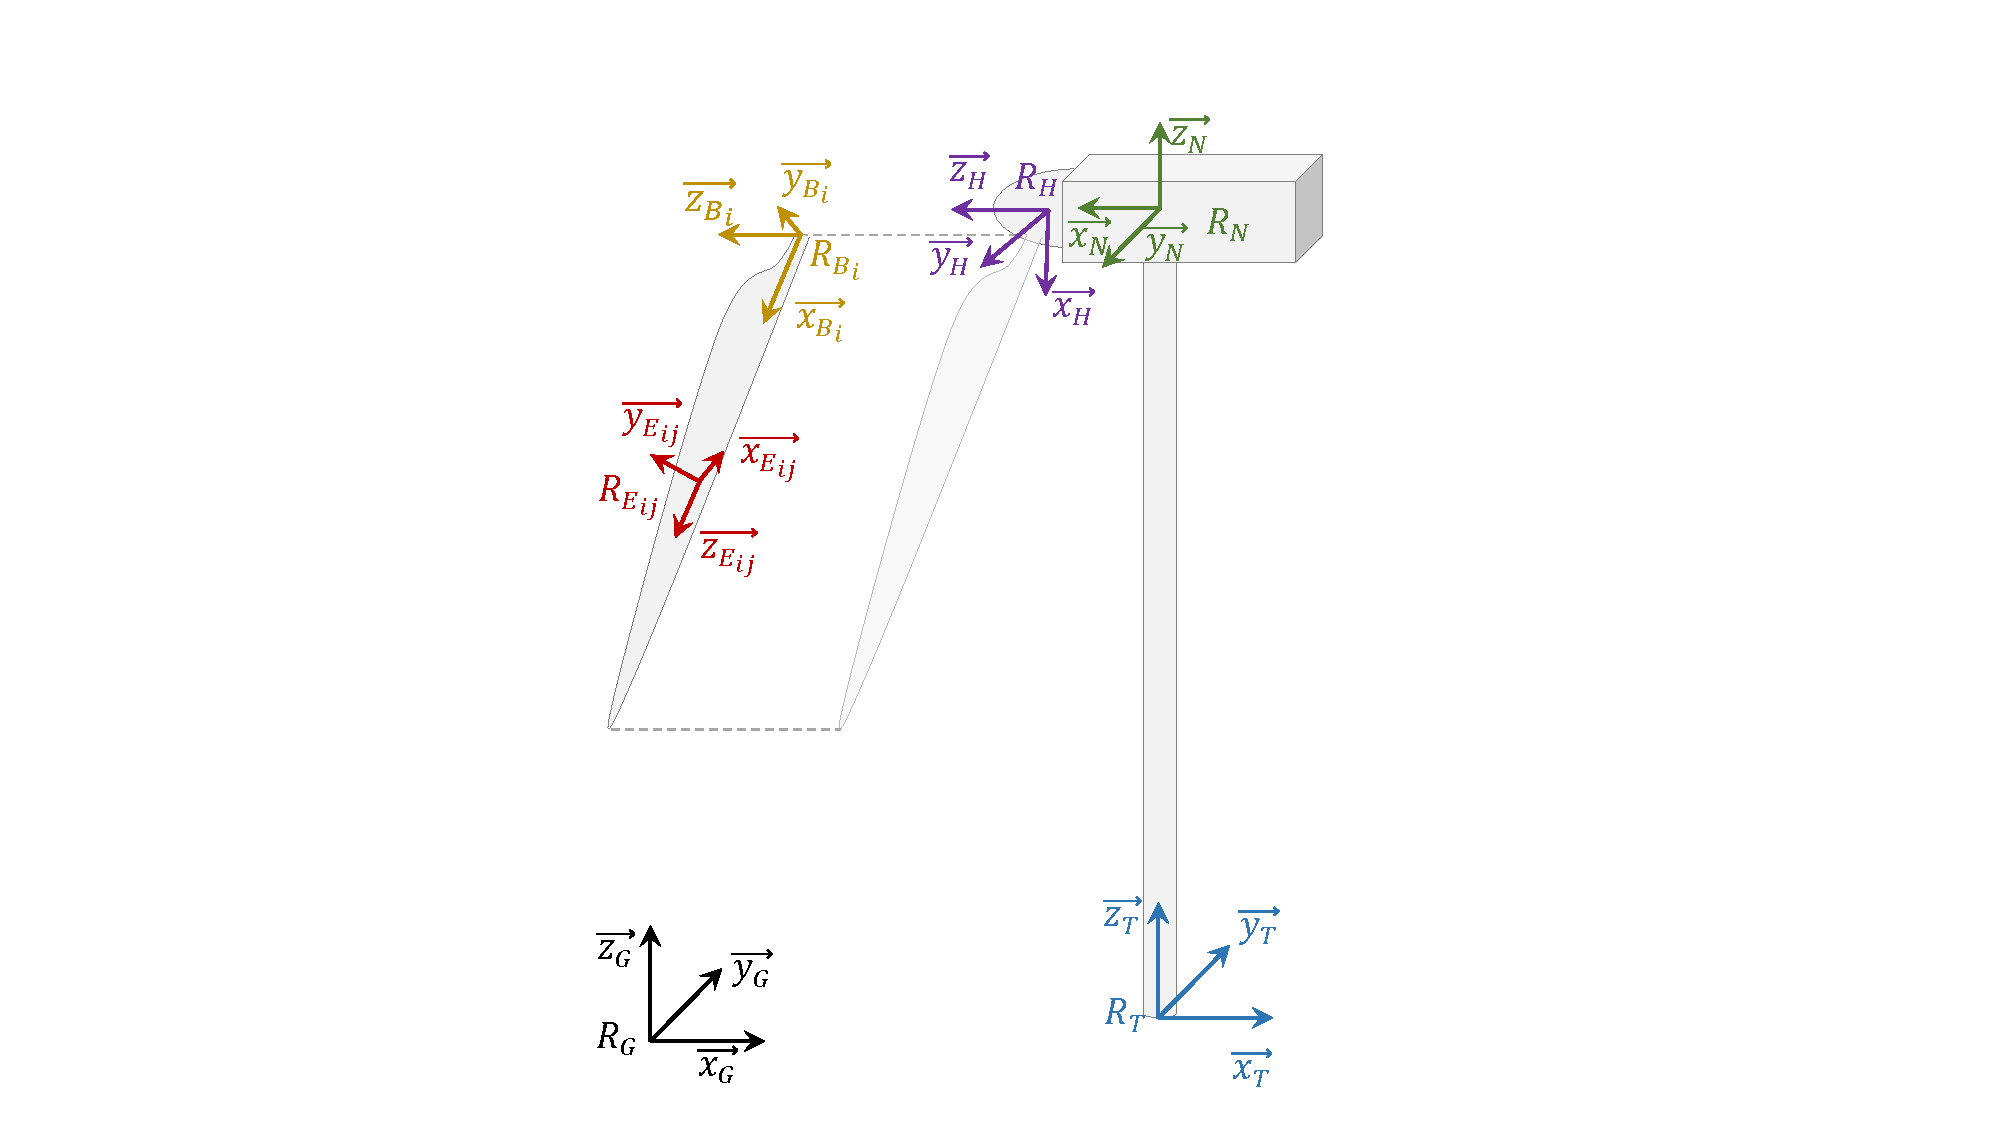
\includegraphics[scale=0.6]{\EPSDIR/Wind_Turbine_fig/CinematiqueRep.pdf}
\caption{Illustration of the frames \citet{joulin2019modelisation}}  
\label{fig:ALrep}
\end{figure}

\subsubsection*{Applying blade element theory}
										

\paragraph*{Determination of $U_{rel}$ and $\alpha$:}
Thanks to the kinematic definition and to the rotation matrices, the determination of the relative wind $U_{rel}$ is almost direct. Indeed, the kinematic relations enable to know the velocity of translation $U^{ij}_{trans}$. Considering the $j^{th}$ elements of the $i^{th}$ blade located in a surrounding volume of air with a velocity $U^{ij}_{wind}$, the relative velocity writes:
\begin{equation}
\label{eq:AL_urel}
\fbox{$
\overrightarrow{U^{ij}_{rel}}_{\vert _{R_{E_{ij}}}} = \mathcal{M}_{R_{E_{ij}} \rightarrow R_{G_{ij}}} \times \overrightarrow{U^{ij}_{wind}}_{\vert _{R_{G_{ij}}}} - \overrightarrow{U^{ij}_{trans}}_{\vert _{R_{E_{ij}}}}
$}.
\end{equation}
And the angle of attack $\alpha$ can be evaluated thanks to:
\begin{equation}
\label{eq:AL_alpha}
\fbox{$
\alpha = tan^{-1} \left( \dfrac{\overrightarrow{U^{ij}_{rel}}_{\vert _{R_{E_{ij}}}} \cdot \overrightarrow{x}}{\overrightarrow{U^{ij}_{rel}}_{\vert _{R_{E_{ij}}}} \cdot \overrightarrow{y}} \right)
$}.
\end{equation}

\paragraph*{Aerodynamic forces:}
By knowing $U_{rel}$ and $\alpha$, the blade element theory can be applied. The aerodynamic forces can be expressed in the aerodynamic frame as:
\begin{equation}
\label{eq:eol_m_alm_eff}	
\fbox{$
\left\lbrace
\begin{array}{ccc}	
dF_{L} = \dfrac{1}{2} \rho S U_{rel}^2 C_L(\alpha),
\\   
\\
dF_{D} = \dfrac{1}{2} \rho S U_{rel}^2 C_D(\alpha).
\\
\end{array}\right.
$}
\end{equation}	

where the lift $C_L$ and drag $C_D$ coefficients are known according to the angle of attack $\alpha$ and the Reynolds number $Re$. The lifting surface $S$, evaluated with the airfoil chord $c$ and the radial width $dr$ ($S = c dr$). By applying a rotation angle $a$, the forces can be expressed in $R_{E_{ij}}$, and then in the global frame by using $\mathcal{M}_{R_{G_{ij}} \rightarrow R_{E_{ij}}}$.

%++++++++++++++++++++++++++++++++
\subsection{Numerical implementation}
%++++++++++++++++++++++++++++++++

The first step of the Actuator Line Method algorithm is to compute the kinematics of the wind turbine. An illustration of the kinematic classes and their discretization is shown in Figure \ref{fig:ALMdiscret}. The kinematic algorithm computes, at each time step, the new positions and velocities of all elements. 
Knowing the position of a blade element, the local wind speed can be extracted. To do so, the wind speed is computed at mass point. Then, it is possible to use the closest value (from the blade element) of the wind, or to interpolate it from the 8-neighborhood cells.
Afterwards, the relative velocity is computed using (\ref{eq:AL_urel}), and the angle of attack $\alpha$ with (\ref{eq:AL_alpha}). The aerodynamic coefficients $C_L$ and $C_D$ are then computed by knowing $\alpha$, from a spline-cubic interpolation of the tabulated input data. Finally, the aerodynamic forces are computed in the aerodynamic frame using (\ref{eq:eol_m_alm_eff}): 
\begin{equation}
\label{eq:eol_m_alm_eff_num}	
\fbox{$
\left\lbrace
\begin{array}{ccc}	
dF_{L} = \dfrac{1}{2} \rho c \Delta r U_{rel}^2 C_L(Re,\alpha),
\\   
\\
dF_{D} = \dfrac{1}{2} \rho c \Delta r U_{rel}^2 C_D(Re,\alpha).
\\
\end{array}\right.
$}
\end{equation}	
A last change of frame enables the projection of these forces to the global momentum budget of Meso-NH. One can note that, for the moment, only the effects of the blades are computed: the nacelle and the tower are neglected. 
\begin{figure}[h]
\centering
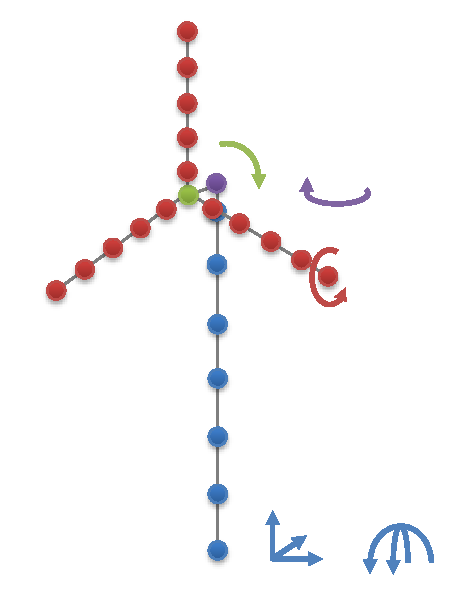
\includegraphics[scale=0.8]{\EPSDIR/Wind_Turbine_fig/ALdiscret.pdf}
\caption{Illustration of the discretised kinematic classes of the ALM. Each color is a different class, and each arrow indicates a possible motion. \citet{joulin2019modelisation}}
\label{fig:ALMdiscret}  
\end{figure}

Note: Special attention must be given to the number of radial (NNB\_BLAELT) elements depending on the mesh used in Meso-NH. To avoid gaps in the mesh and ensure a proper distribution of efforts, it is recommended to have:
\begin{equation}
NNB\_RADELT > \dfrac{2R}{\min(\Delta x, \Delta y, \Delta z)}
\end{equation}
where $R$ is the radius of the rotor, and $\min(\Delta x, \Delta y, \Delta z)$ is the smallest dimension of the Meso-NH mesh at the rotor level.


%++++++++++++++++++++++++++++++++
\subsection{Additional implementations}
%++++++++++++++++++++++++++++++++
\subsubsection*{1D linear smearing}
It is possible to use the 1D linear smearing mentionned in \ref{sss:1dsmearADNR}.

\subsubsection*{3D linear smearing}
It is possible to use the 3D linear smearing mentionned in \ref{sss:3dsmearADNR}.

\subsubsection*{Tip loss correction}
\label{sss:tiplossALM}

An over-estimation of loads is commonly predicted by the Actuator Line Method. It appears when the mollification (smearing) or the resolution are not adequate to generate de tip vortices and so the tip losses. 
To overcome this issue, the community usually applies the tip loss correction of \citet{glauert1935airplane}, explainded in \ref{sss:tiplossADR}. It allows a better prediction of the loads (\citet{mikkelsen2003actuator} or \citet{shen2005tip}).
\medbreak
One can note that in the ALM, the number of blade is finite and this correction should not be used. Some specific corrections could be implemented, as shown by \citet{breton2008study}. Besides, a better distribution of forces is also possible as proposed by \citet{churchfield2017advanced}. 
As Meso-NH is a meteorological tool, the resolution might be too large compared to the guidelines recommanded for the ALM \citet{jha2014guidelines}. Then, the tip loss correction is applied by default in Meso-NH (LTIPLOSSG = .TRUE.).

\subsubsection*{Time-splitting method}
\label{sss:time_splitting}
In order to save computational cost, a time-splitting method has been introduced \citet{joulin2020theactuator}. This method is also called Actuator Sector Method \citet{Storey2015}. If this technique allows for computational time savings, it should be used with caution, as the results may be degraded (see \citet{joulin2019modelisation, jezequel2022simulations}).
The Courant-Friedrichs-Lewy (CFL) criterion of Meso-NH imposes a time step $\Delta t_{MNH}$. The criterion writes:
\begin{equation}	
n_{CFL} =  c \dfrac{\Delta t_{MNH}}{min(\Delta x,\Delta y,\Delta z)},
\label{eq:MNH_CLF}
\end{equation}  
where $c$ is the flow velocity, and  $\Delta x$, $\Delta y$, $\Delta z$ the cell sizes. In Meso-NH, $n_{CFL} < 3$ is imposed according to the scheme used.
\medbreak
Nevertheless, the ALM often requires a smaller time step in order to ensure that a blade element point will not skip a mesh cell during this time step. The criterion for the Actuator Line Method time step $ \Delta t_{ALM}$ can thus be expressed as:
\begin{equation}
\Delta t_{ALM} \leqslant \dfrac{min(\Delta x,\Delta y,\Delta z)}{\Omega r_{tip}},
\label{eq:dt_alm}
\end{equation}
where $\Omega$ is the angular velocity of the wind turbine, and $r_{tip}$ the tip radius of the blade.
\medbreak
Because Meso-NH does not need such a small time step, a $\Delta t_{MNH}$ respecting the CFL criterion is preserved. On the other side, the ALM algorithm is called $N_{split}$ times over this duration in order to respect the ALM time step criterion (eq. (\ref{eq:dt_alm})) and to reduce by $N_{split} - 1$ the number of iterations from the LES solver.
\medbreak
\begin{figure}[h]
\centering
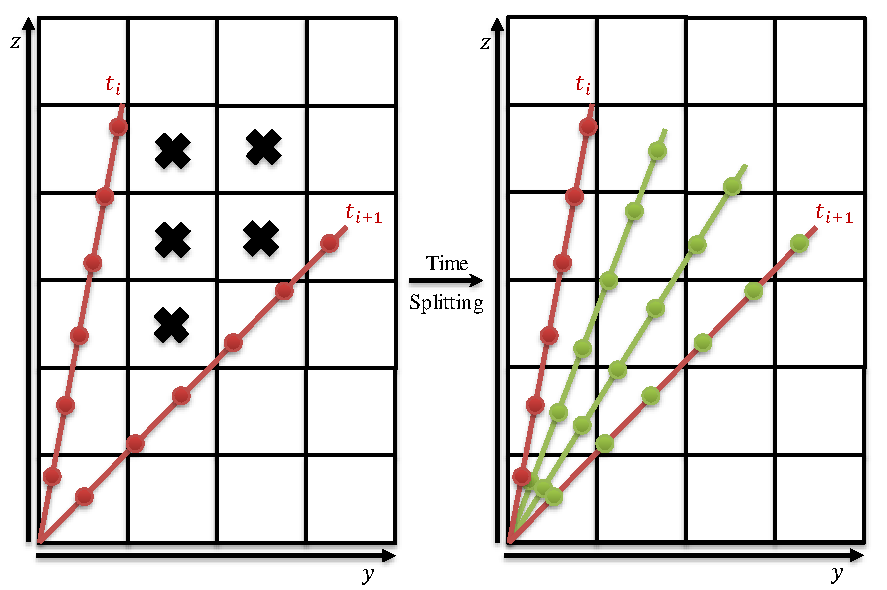
\includegraphics[scale=0.8]{\EPSDIR/Wind_Turbine_fig/Time_Splitting.pdf}
\caption{Illustration of time-splitting method, for $N_{split} = 3$. \citet{joulin2019modelisation}}
\label{fig:timesplit}  
\end{figure}
The method is illustrated in Figure \ref{fig:timesplit}. The red lines indicate blade positions at $t_{i}$ and $t_{i+1}$. The red dots indicate blade elements. The black crosses on the left Figure show the cells missing the blade passage. On the right, the time-splitting method enables to get the history of the blade motion (green lines and dots) to compute to aerodynamic forces.

One can note that during a Meso-NH time step, the wind field is frozen. In the end, for each blade element point, the applied force is the aerodynamic force evaluated by the ALM divided by $N_{split}$ to respect the momentum budget over $\Delta t_{MNH}$.


%%%%%%%%%%%%%%%%%%%%%%%%%%%% BIBLIOGRAPHY %%%%%%%%%%%%%%%%%%%%%%%%
\begin{btSect}{3-10-WindTurbine}
\section{References}
\btPrintCited
\end{btSect}
%%%%%%%%%%%%%%%%%%%%%%%%%%%% BIBLIOGRAPHY %%%%%%%%%%%%%%%%%%%%%%%%

%%%%%%%%%%%%%%%%%%%%%%%%%%%%%%%%%%%%%%%%%%%%%%%%%%%%%%%%%%%%%%%%%%%%%%%%%%%%%%%%%%%%%%%%%%%%%
% CONTRIBUTION TO THE MESONH BOOK3: "Blaze fire model"
% Authors : Aurélien Costes
% Original : May, 2021
% Update
%%%%%%%%%%%%%%%%%%%%%%%%%%%%%%%%%%%%%%%%%%%%%%%%%%%%%%%%%%%%%%%%%%%%%%%%%%%%%%%%%%%%%%%%%%%%%

\chapter{Blaze fire model}
\minitoc

%%%%%%%%%%%%%%%%%%%%%%%%%%%%%%%
\section{Introduction}
%%%%%%%%%%%%%%%%%%%%%%%%%%%%%%%

The fire's existence is represented in the atmospheric model by the latent and sensible heat fluxes at the surface, and the impact of the atmosphere on the fire's behavior is represented in the fire model by the surface wind in \MNH-\Blaze.
The role of the \Blaze{} model can be summarized as follows~:
\begin{itemize}
	\item identify the position of the fire front at a time $t$,
	\item communicate with \MNH{} to retrieve surface wind data at time $t$,
	\item compute the normal rate of spread of the fire front $\mathcal R$ at this time $t$ as a function of meteorological and environmental factors,
	\item to make the fire front move on the terrain surface up to the time $t+\Delta t$,
	\item calculate the latent and sensible heat fluxes induced by the fire between the instants $t$ and $t+\Delta t$,
	\item communicate with \MNH{} to provide heat flux data for the period $[t,t+\Delta t]$,
	\item operate in a massively parallel environment by using the parallelization tools of \MNH.
\end{itemize}

The Blaze fire model features the following components: \textit{i)} an Eulerian two-dimensional front-tracking model that relies on a level-set (LS) method and uses a description of the local rate of spread based on Balbi’s formulation \citep{Balbi2009}; and \textit{ii)} a flux parametrisation that estimates the spatial distribution and intensity of the surface latent and sensible heat fluxes. If Blaze is embedded in an atmospheric model, these heat fluxes act as surface boundary conditions to solve the atmospheric flow perturbed by the fire.

The interested reader is strongly advised to read the thesis of Aurélien COSTES and the original paper of Blaze in addition to this technical note \citep{costes2021subgrid}.

%%%%%%%%%%%%%%%%%%%%%%%%%%%%%%%
\section{Level-set method for fire spread}
%%%%%%%%%%%%%%%%%%%%%%%%%%%%%%%

%%%%%%%%%%%%%%%%%%%%%%%%%%%%%%%
\subsection{Fire mesh}
%%%%%%%%%%%%%%%%%%%%%%%%%%%%%%%

The LS method is used to propagate the time-evolving fireline on a two-dimensional horizontal plane $(x, y)$. The two-dimensional fire grid is defined with respect to the resolution of the atmospheric data.
Since the fireline propagation is a subgrid-scale process with respect to the atmosphere, the atmospheric mesh is divided into $\Gamma_x$ cells in the $x$-direction and $\Gamma_y$ cells in the $y$-direction to form the fire mesh in Blaze.
A distinction is therefore made between the atmospheric surface mesh, referred to as ``atmospheric mesh'', of resolution $(\Delta x, \Delta y$), and the fire mesh of resolution $(\Delta x_f, \Delta y_f$) with $\Delta x_f = \Delta x / \Gamma_x$ and $\Delta y_f = \Delta y / \Gamma_y$.

\bigskip

From a technical point of view, it means that the fire mesh is a 2D array of size $(\Gamma_x N_x, \Gamma_y N_y)$ where $N_x$ and $N_y$ represent the size of the atmospheric mesh in $x$ and $y$ directions respectively.
However, this 2D grid size is not supported by the parallelization paradigm of \MNH{} which needs a 2D array of size $(N_x, N_y)$.
Therefore, every fire related array which is normally of size $(\Gamma_x N_x, \Gamma_y N_y)$ shall be stored as a 3D array of size $(N_x, N_y, \Gamma_x \Gamma_y)$.
The 3D format arrays are not very convenient for gradient operators.
Fire related fields are stored in this 3D format in output files which is not very convenient either for post processing. 
Two functions are then defined to switch from one representation to another.

\medskip

The first one uses 3D representation indexes $(i,j,k)$ to compute 2D representation indexes $(l, m)$. It defines temporary variables $a$ and $b$.

\begin{align}
  b &= (k-1) \div \Gamma_x + 1 \nonumber \\
  a &= k - (b-1)\Gamma_x \nonumber \\
  l &= (i-1)\Gamma_x + a \\
  m &= (j-1)\Gamma_y + b 
\end{align}
where $\div$ is the euclidian division.

\medskip

The second one uses 2D representation indexes $(l, m)$ to compute 3D representation indexes $(i,j,k)$. It defines temporary variables $a$ and $b$.

\begin{align}
	a &= l - (i-1)\Gamma_x \nonumber \\
	b &= m - (j-1)\Gamma_y \nonumber \\
	i &= \left \lceil \frac{l}{\Gamma_x} \right \rceil \\
	j &= \left \lceil \frac{m}{\Gamma_y} \right \rceil \\
	k &= (b-1)\Gamma_x + a
\end{align}

These functions are commonly used in the code in three steps: \textit{i)} switch an fire related array from 3D to 2D representation, \textit{ii)} use an operator (gradient for example) on the 2D array, \textit{iii)} switch the result of the operator from 2D to 3D representation.

For post processing purposes, the two functions are available in the Pyrolib package.

%%%%%%%%%%%%%%%%%%%%%%%%%%%%%%%
\subsection{Governing equation}
%%%%%%%%%%%%%%%%%%%%%%%%%%%%%%%
\label{sec:governingeq}

In Blaze, the LS function $\phi \equiv \phi(x,y,t)$ is not a signed distance but rather a bounded function $0 \leqslant \phi \leqslant 1$, where the contour line $\phi = 0.5$ is identified as the fire front; $\phi > 0.5$ represents burnt vegetation; and $\phi < 0.5$ represents unburnt vegetation at a given time $t$. The LS field is transported at the rate of spread $\mathcal R$ and satisfies the following Hamilton-Jacobi equation:
\begin{equation}
\dpar{\phi}{t}{} = \mathcal R \left (|\nabla \phi | + \epsilon_\phi \widetilde \Delta \phi \right )
\label{eq:lveq}
\end{equation}
where $\nabla \phi = \left ( \dpar{\phi}{x}{}, \dpar{\phi}{y}{} \right )$ is the LS gradient, $\widetilde \Delta \phi = \left ( \Delta x_f\,\dpar{\phi}{x^2}{2} + \Delta y_f\,\dpar{\phi}{y^2}{2} \right )$ is the fire-mesh-size-proportional Laplacian, $\epsilon_\phi \widetilde \Delta \phi$ is the artificial viscosity term to ensure numerical stability, and $\mathcal{R}$ represents the speed projected onto the normal direction $\uvec n$ to the fireline, 
$\uvec n = -\nabla \phi/|\nabla \phi |$. $\mathcal{R}$ is evaluated using Balbi's rate-of-spread parameterization \citep{Santoni2011}.
Numerical tests have shown that $\epsilon_\phi = 0.1$ gives satisfactory results.

\medskip

In \Blaze, the Hamilton-Jacobi equation (Equation~\ref{eq:lveq}) is solved numerically using a third-order Runge-Kutta scheme in time and a third-order WENO (\emph{Weighted Essentially Non-Oscillatory}) scheme in space (RK3-WENO3). A first order WENO method and the same RK schemes as for MesoNH are also available.

\medskip

Due to the potential heterogeneity of the fuel parameters that may affect the stability of the numerical schemes, an artificial viscosity is added to the ROS computation (in addition to the one added to the level-set $\phi$ function) as follows:
\begin{enumerate}
	\item At each point on the fire grid, a temporary rate of spread, denoted $\mathcal R^*$, is calculated from Balbi's analytical formulation.
	\item The modified Laplacian operator is computed on the temporary field, $widetilde \Delta \mathcal R^*$, subject to local variations due to heterogeneities in the input parameters~:
\begin{equation}
\mathcal R = \mathcal R^* + \varepsilon_{\mathcal R} \widetilde \Delta \mathcal R^*,
\end{equation}
where $\varepsilon_{\mathcal R}$ is the viscosity coefficient on the rate of spread which is set by default to 0.1. This value was considered reasonable in view of numerical tests not shown here.
	\item This smoothing operation is repeated a second time in order to obtain a satisfactory result on the rate of spread $\mathcal R$, that is:
\begin{equation}
  \mathcal R = \mathcal R^* + \varepsilon_{\mathcal R} \widetilde \Delta \mathcal R^* + \varepsilon_{\mathcal R}  \widetilde \Delta \left ( \mathcal R^* + \varepsilon_{\mathcal R} \widetilde \Delta \mathcal R^* \right ).
\end{equation}
\end{enumerate}

%%%%%%%%%%%%%%%%%%%%%%%%%%%%%%%
\subsection{Wind interpolation}
%%%%%%%%%%%%%%%%%%%%%%%%%%%%%%%

In order to compute the rate of spread on the fire mesh, we need to interpolate the wind speed from the atmospheric mesh to the fire mesh. We need to compute $U_0$ defined by:
\begin{equation}
  U_0 = \uvec U \cdot \uvec n,
\end{equation}
where $\uvec U$ is the wind vector at the fire front and $\uvec n$ the fire front normal vector. As $\uvec n$ is a 3D vector, every component of the wind needs to be interpolated.

\subsubsection{Vertical interpolation}

For now, there is no vertical interpolation of the wind in \Blaze.
The horizontal wind $(u, v)$ is taken at the first vertical level (excluding the halo).
The vertical wind is linearly interpolate at the same level between the ground and the first vertical level (excluding the halo).
The lack of independence between the mesh and the interpolation method is a real problem for the model.
This development should be a one of the priorities of the community. 

\subsubsection{Horizontal interpolation}

The simplest horizontal interpolation method is to distribute the wind from one atmospheric cell to all the fire cells included in it, which is equivalent to considering a uniform wind in an atmospheric cell. This method is used when LINTERPWIND is set to False. It can lead to discontinuities in the rate of spread and is not recommended.

\medskip

When LINTERPWIND is set to True, a 2D interpolation of the wind $(u,v, w)$ is applied.

The first step in this method is to linearly interpolate each wind component at the corners of the considered atmospheric mesh, represented by the white circles in Figure~\ref{fig:windinterpH}. For example, for the bottom right point of the considered atmospheric mesh, the intermediate wind is computed as follows~:
\begin{equation}
\uvec u_1 = (u_1,v_1) = \frac{1}{2} (u_{ij} + u_{ij-1},v_{ij} + v_{i-1j}).
\end{equation}

The second step consists in bilinearly interpolating the wind $\uvec u_{ijk}$ at each fire cell indexed with $k \in [1,\Gamma_x \Gamma_y]$ and contained in the considered atmospheric mesh, labeled by the indexes $(i,j)$ from the values $\uvec u_1$, $\uvec u_2$, $\uvec u_3$, and $\uvec u_4$~:
\begin{equation}
	  \uvec u_{ijk} = \frac{1}{(\Gamma_x +1 ) (\Gamma_y +1)}  \bigg [ m(l \uvec u_3 + (\Gamma_x + 1 - l) \uvec u_4) + (\Gamma_y + 1 - m)(l \uvec u_2 + (\Gamma_x +1 - l) \uvec u_1) \bigg ],
\end{equation}
with
\begin{align}
  m &= (k-1) \div \Gamma_x + 1,  \\
  l &= k - (m-1)\Gamma_x,
\end{align}
where $\div$ is the Euclidean division.

\subsubsection{Time-based smoothing}

For very rapidly varying wind intensity, the temporal signal given to the rate-of-spread parameterization can be smoothed by using a moving average method. The recursive Exponential Weighted Averaging Method is used in \Blaze. The interest quantity $s_n$ given to \Blaze{} is computed from the previous time step $s_{n-1}$ and the interpolated wind computed by \MNH{} $u_n$ as:
\begin{equation}
  s_n = s_{n-1} + \beta (u_n - s_{n-1}),
\end{equation}
where $\beta \in [0, 1]$ is a control parameter.
The value of $\beta$ is computed by:
\begin{equation}
  \beta = \frac{2}{1 + \left \lceil \frac{\tau}{\Delta t} \right \rceil},
\end{equation}
where $\tau$ [\second] is the averaging time (the same time constant one would find in a simple averaging method), and $\Delta t$ is the \MNH{} time step.

The time-based smoothing can be activated by LWINDFILTER=.TRUE.. The time constant $\tau$ of the filter is set by XEWAMTAU (default valut: 20\second).

%%%%%%%%%%%%%%%%%%%%%%%%%%%%%%%
\subsection{Slope impact on rate of spread}
%%%%%%%%%%%%%%%%%%%%%%%%%%%%%%%

The Section~\ref{sec:governingeq} described the governing equation for the level-set method on a flat and uniform cartesian grid.
However, the terrain is not always flat and the rate of spread parameterization needs to take into account the slope.

\subsubsection{vector space definition}

Let's consider here four vector bases. The orthonormal reference base of the atmospheric model $(\uvec e_x, \uvec e_y, \uvec e_z)$. It contains for example the wind $\uvec U$. There is also the contravariant basis $(\uvec{\hat e}_x, \uvec{\hat e}_y , \uvec{\hat e}_z)$ which corresponds to the deformed basis of the atmospheric mesh. 

\smallskip

Then, we find the basis of the flame plane $(\uvec n, \uvec p, \uvec q$) with $\uvec n$ the normal to the front parallel to the surface, $\uvec p$ the normal to the surface and $\uvec q$ the vector product of the two previous vectors.

\smallskip

Let us project this basis on the horizontal surface which constitutes the basis for the level set $(\uvec{\tilde n}, \uvec{\tilde p}, \uvec{\tilde q})$. These vectors are determined by $\uvec{\tilde n} \cdot \uvec n = \cos \alpha$, where $\alpha$ is the slope in the propagation direction. In this case, $\uvec{\tilde p} = \uvec e_z$ and $\uvec{\tilde q} = \uvec q$. This basis corresponds to the rotation of angle $- \alpha$ according to the vector $\uvec q$ of the basis $(\uvec n, \uvec p, \uvec q)$.

\subsubsection{Vector composition}

The purpose is to implement the effect of slope on the rate of spread $\mathcal R$ of the Balbi model.
As a reminder, the ROS is affected by the wind and the slope in a single expression depending on the value of the \textit{tilt angle} of the flame $\gamma$.
This angle corresponds to the composition of the mid-flame wind vector $\uvec U_0$ and the vertical velocity vector in the flame $\uvec v_f$:
\begin{equation}
  \uvec V = \uvec U_0 + \uvec v_f.
\end{equation}
The $\gamma$ angle is then defined as
\begin{equation}
  \tan \gamma = \frac{\uvec V \cdot \uvec n}{\uvec V \cdot \uvec p}.
\end{equation}
The wind vector is by definition collinear to the front normal
\begin{equation}
  \uvec U_0 = U_0 \uvec n.
\end{equation}
The vertical velocity in the flame is by definition collinear with the vertical direction
\begin{equation}
  \uvec v_f = v_f \uvec e_z.
\end{equation}

In \citep{Santoni2011}, the vertical velocity along the surface normal $v_0$ is known as a function of the other model parameters.
Moreover, \cite{Santoni2011} shows that
\begin{equation}
  v_f = \frac{v_0}{\cos \alpha}. 
\end{equation}
Decomposing $\uvec e_z$ in the flame plane basis and using the previous relation, one gets 
\begin{equation}
  \uvec V = (U_0 + v_0 \tan \alpha) \uvec n + v_0 \uvec p.
\end{equation}
Therefore, it is possible to write 
\begin{equation}
  \tan \gamma = \tan \alpha + \frac{U_0}{v_0}.
  \label{eq:tangamma}
\end{equation}

\subsubsection{Computation of the base spaces}

It is necessary to compute a few basis vectors to determine $\gamma$. In particular, the level set propagation is done on an imaginary horizontal plane of basis $(\uvec e_x, \uvec e_y)$.
From $\uvec \nabla \phi$, we can determine $\uvec{\tilde n}$.
It is then necessary to calculate $\alpha$, $\uvec n$ and $U_0$.

\medskip

The slope is a two-dimensional vector that can be expressed in several bases. A natural basis, already used in many models, consists of two angles $\alpha_s$ and $\alpha_a$, representing the angle of steepest slope and the direction of the face with respect to North, respectively.
The second option is to use a projection of the slope vector on an orthonormal basis, typically $(\uvec e_x, \uvec e_y)$.

\medskip

For \MNH-\Blaze, the slope can be determined by two methods:
\begin{itemize}
  \item through a height map on the atmospheric grid, $z(x,y)$, or the fire grid, $z(x_f,y_f)$,
  \item or a map of angles $\alpha_s$ and $\alpha_a$ on the fire grid.
\end{itemize}
The two representations are strictly equivalent but the numerical use of angles requires the use of many trigonometric and non-linear functions which has a very important numerical cost.
Whenever possible, it is better to work with vector projection, which only requires scalar products (\textit{i.e.} a product of vectors component by component, which is easily vectorized by the machine).

We therefore set up a calculation strategy based on the height map and the components of the orographic gradient. 

\paragraph{Computation of the orographic gradient}
The expression of the components of the orographic gradient $\uvec \nabla z$, noted $\uvec h$ at the center of the atmospheric cell $(i,j)$ is given by:
\begin{equation}
  \begin{split}
  	\uvec \nabla z \cdot \uvec e_x = h_{i,j}^{x,a} &= \frac{ z_{i+1,j-1} - z_{i-1,j-1} + 2 (z_{i+1,j}-z_{i-1,j}) + z_{i+1,j+1} - z_{i-1,j+1}}{8 \Delta x}, \\
  	\uvec \nabla z \cdot \uvec e_y = h_{i,j}^{y,a} &= \frac{z_{i-1,j+1} -z_{i-1,j-1} + 2 (z_{i,j+1}-z_{i,j-1}) + z_{i+1,j+1} - z_{i+1,j-1}}{8 \Delta y}. \\
  \end{split}
\end{equation}

As for the interpolation of the wind, we interpolate at the corners of the atmospheric mesh, noted $\llcorner$. There are thus $(N_x +1, N_y+1)$ interpolated slopes. For the $x$ component, it is defined by:
\begin{equation}
  h_{i,j}^{x,a\llcorner} = \frac{h_{i,j}^{x,a} + h_{i-1,j}^{x,a} + h_{i,j+1}^{x,a} + h_{i+1,j+1}^{x,a}}{4}.
\end{equation}
Same on the $y$ component.

Finally, we interpolate the orographic gradient components on the fire grid with the same approach as for the wind components. 

\paragraph{Computation of the front normal on the surface plane}
For a particular fire cell, the components of the orographic gradient allow to determine two director vectors of the plane forming the mean surface of fire cell.
\begin{align}
	\uvec s_1 &= ( 1, 0, h_x ), \\
	\uvec s_2 &= (0,1,h_y).
\end{align}
The normal vector $\uvec n$ lies in this plane and has for projection on the horizontal plane the vector $\uvec{\tilde n}$ whose components are known as
\begin{equation}
  \uvec{\tilde n} = \frac{1}{\| \uvec \nabla \phi \|} (\uvec \nabla_x \phi, \uvec \nabla_y \phi, 0 ).
\end{equation}
$\uvec n$ is therefore a linear combination of the two director vectors
\begin{equation}
  \uvec n = a \uvec s_1 + b \uvec s_2.
\end{equation}
However, $\uvec n$ shares its components on $x$ and $y$ with $\uvec{\tilde n}$, which can be written
\begin{equation}
  \begin{cases}
  	n_x = a = \tilde n_x \\
  	n_y = b = \tilde n_y \\
  	n_z = a h_x + b h_y \\
  \end{cases}
\end{equation}
This allows us to write that the angle of the slope in the direction of propagation $\alpha$ respects
\begin{equation}
  \tan \alpha = \frac{\tilde n_x h_x + \tilde n_y h_y}{\sqrt{\tilde n_x^2 + \tilde n_y^2}}.
\end{equation}
However, $\uvec{\tilde n}$ is a unit vector which implies that its norm is 1. Therefore we get 
\begin{equation}
  \tan \alpha = \tilde n_x h_x + \tilde n_y h_y.
  \label{eq:alphadef}
\end{equation}
This is equivalent to calculating $\uvec{\tilde n} \cdot \uvec h $ in the horizontal plane. . This scalar produc can be used to directly calculate the slope term in the equation~\eqref{eq:tangamma}. 
With this definition, $\uvec n$ is not a unit vector. This property will be very useful when projecting the wind. We then normalize the vector $\uvec n$. The norm is denoted by $\mathcal N$.
\begin{equation}
  \mathcal N^2 = 1 + \tilde n_x^2 h_x^2 + \tilde n_y^2 h_y^2.
\end{equation}

We finally change the definition of the normalized $\uvec n$ vector:
\begin{equation}
  \begin{cases}
  	n_x = \frac{\tilde n_x}{\mathcal N}, \\
  	n_y = \frac{\tilde n_y}{\mathcal N}, \\
  	n_z = \frac{\tilde n_x h_x + \tilde n_y h_y}{\mathcal N}. \\
  \end{cases}
\end{equation}

\subsubsection{Rate of spread projection on the horizontal plane}

We compute $\mathcal R$ according to the front normal on the surface plane
\begin{equation}
  \uvec{\mathcal R} = \mathcal R \uvec n.
\end{equation}
We want to compute the projection of $\uvec{\mathcal R}$ on $\uvec{\tilde n}$.
\begin{equation}
  \widetilde{\mathcal R} = \mathcal R \uvec n \cdot \uvec{\tilde n} = \mathcal R \cos \alpha
\end{equation}
Numerically, we already know the value of $\tan \alpha$ but not the value of the angle. To compute this projection it is necessary to compute $\cos (\arctan (\tan \alpha))$ which costs on average 3 times more than using the expression $\cos \alpha = 1 /\sqrt{1 + \tan^2 \alpha}$.
To optimize this calculation we have
\begin{equation}
  \widetilde{\mathcal R} = \mathcal R \frac{1}{\sqrt{1 + \tan^2 \alpha}}.
\end{equation}

%%%%%%%%%%%%%%%%%%%%%%%%%%%%%%%
\section{Heat fluxes parameterizations}
%%%%%%%%%%%%%%%%%%%%%%%%%%%%%%%

In \Blaze, sensible and latent heat fluxes computation is based on energy reservoir. Each fire cell constitutes a sensible and latent energy reservoir called Available Sensible Energy (ASE) and Available Water Content (AWC), respectively, based on fuel properties. Then, the heat flux parameterization is the temporal description of how fast this reservoir is emptying. These parameterizations for sensible and latent heat fluxes are noted $\psi_h(t, t^a(\uvec x))$ and $\psi_w(t, t^a(\uvec x))$, respectively. They are functions of time and arrival time $t^a$ at the position $\uvec x$.
In order to improve the spatial description of heat flux, these functions are moderated by the subgrid surface that is currently burning in the fire cell $\mathcal S (\uvec x, t)$. 
Then, the surface fluxes are given by:
\begin{align}
	\Psi_h (\uvec x, t) &= \psi_h(t, t^a(\uvec x)) \mathcal S (\uvec x, t), \\
	\Psi_w (\uvec x, t) &= \psi_w(t, t^a(\uvec x)) \mathcal S (\uvec x, t).
\end{align}
$\Psi_h$ [\watt\,\rpsquare\meter] is the sensible heat flux, and $\Psi_w$ [\kilo\gram\,\reciprocal\second\,\rpsquare\meter] is the water vapor flux. 

\textbf{The complete description of the current flux models and the EFFR method are given in \citep{costes2021subgrid}.}

The paper will give the method used to compute surface heat flux. However, these surface fluxes are distributed over several vertical level in \MNH{} as volume source terms. For sensible and latent heat fluxes, these source terms are written, respectively as:
\begin{align}
	\dpar{\rho_{dref} \theta}{t}{} &= Q_h + \frac{\mathcal F_h}{C_{ph}}, \\
	\dpar{\rho_{dref} r_v}{t}{} &= Q_w + \mathcal F_w.
\end{align} 
$Q_h$ represents all the others processes in the \MNH{} energy balance equation (advection, humidity correction, phase change, etc.), $\mathcal F_h$ [\watt\,\rpcubic\meter] is the volume source term from \Blaze, and $C_{ph}$ is the specific heat of moist air. 
$Q_w$ represents all the others processes in the \MNH{} water vapor conservation equation, and $\mathcal F_w$ [\kilo\gram\,\reciprocal\second\,\rpcubic\meter] is the source term from \Blaze.

The surface terms computed by \Blaze{} are distributed by an exponential law. For the sensible heat flux, this distribution is written as:
\begin{equation}
  \mathcal F_h (z) = \mathcal F_h^0 \exp \left ( - \frac{z}{z_f} \right ),
\end{equation}
where $\mathcal F_h (z)$ is the volume source term, $\mathcal F_h^0$ is the value at the surface, and $z_f$ a characteristic height used a parameter (XFLUXZEXT in the namelist). To determine $\mathcal F_h^0$, we add a contraint on the integral of the volume source term:
\begin{equation}
  \int_0^{z_{\mathrm{max}}} \mathcal F_h (z) \, \mathrm d z = \Psi_h.
\end{equation}
The parameter $z_{\mathrm{max}}$ is the maximum injection height (XFLUXZMAX in the namelist). Numerically, the discretised volume source term $\mathcal F_k$ is the mean value of $\mathcal F_h (z)$ in the considered cell, noted $k$. It is computed as:
\begin{equation}
\mathcal F_k =
\begin{cases}
\frac{psi_h}{\Delta z_k} \frac{\exp \left ( - \frac{z_{k-1/2}}{z_f} \right ) - \exp \left ( - \frac{\min \left ( z_{k+1/2},z_{\mathrm{max}} \right )}{z_f} \right )}{1 - \exp \left ( -\frac{z_{\mathrm{max}}}{z_f}\right )}  & \text{if } z_{k-1/2} < z_{\mathrm{max}}, \\
0 & \text{else}. \\
\end{cases}
\end{equation}
Flux vertical levels are noted with semi-integer indexes and mass vertical levels are noted with integer indices $z_k = \frac{z_{z - 1/2} + z_{k+1/2}}{2}$. Then the vertical cell size is $\Delta z = z_{z + 1/2} - z_{z - 1/2}$.



%%%%%%%%%%%%%%%%%%%%%%%%%%%%%%%
\section{Coupling modes}
%%%%%%%%%%%%%%%%%%%%%%%%%%%%%%%

This section presents the three coupling modes between \Blaze{} and \MNH.
For each mode, the coupling variables are exchanged at each atmospheric time step.

\begin{figure}
	\centering
	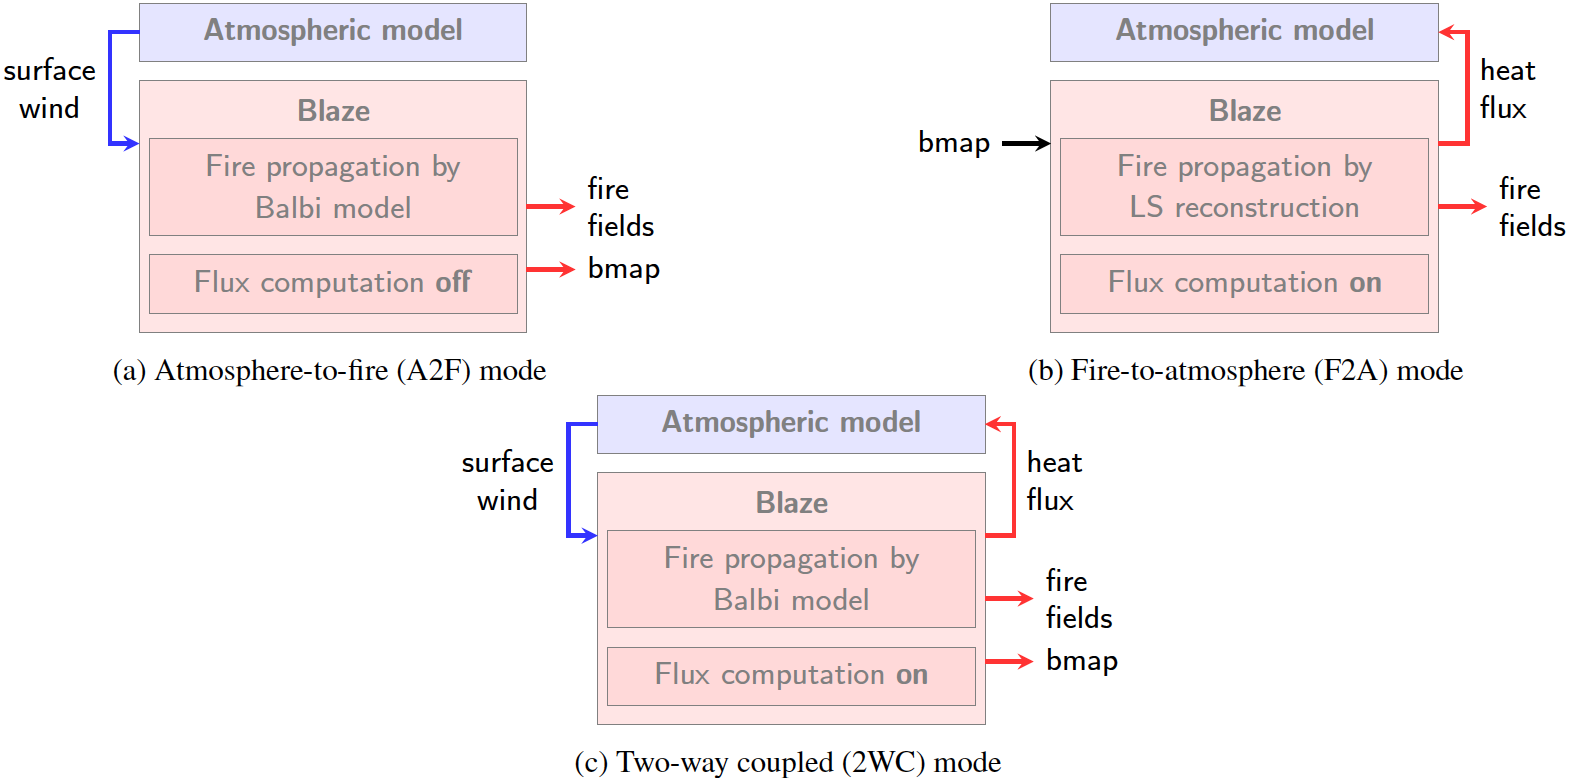
\includegraphics[width=\textwidth]{EPS/couplingmodes.png}
	\caption{Two-way coupled (2WC) mode}
  	\label{fig:2WCMode}
\end{figure}

%%++++++++++++++++++++++++++++++++
\subsection{Forced atmosphere-to-fire mode (forced mode)}
\label{ssec:cpl1A2F}
%%++++++++++++++++++++++++++++++++

In the forced (A2F) mode (Fig.~\ref{fig:2WCMode}a), the fire spread is affected by the atmospheric flow but the wind conditions are not disturbed by the fire. Blaze requires the wind conditions near the surface from an atmospheric model to compute the Balbi's rate of fire spread but no heat flux computation is needed. As output, Blaze provides the burning map and the fire related fields (LS function $\phi$, rate of spread $\mathcal R$, wind contribution to the rate of spread $(\mathcal R - \mathcal R_0)$, ASE and AWC).

%%++++++++++++++++++++++++++++++++
\subsection{Forced fire-to-atmosphere mode (fire replay mode)}
\label{ssec:cpl1F2A}
%%++++++++++++++++++++++++++++++++

To perform numerical convergence tests or investigate the atmospheric response to fire energy release, it is of primary interest to run simulations from a predetermined fire. This fire replay (F2A) mode (Fig.~\ref{fig:2WCMode}b) takes as input an existing burning map (obtained from simulation or observation), and computes latent and sensible heat fluxes to be injected into the atmospheric model. The fire spread model component is not used. Instead, a temporal reconstruction of the LS function $\phi$ is performed from information contained in the burning map. This is done through a sigmoid function of parameter $\lambda$:
\begin{equation}
  \phi (x,y,t) = \frac{1}{1+ e^{-\lambda (t - t^a (x,y)) }}
  \label{eq:sigmoid}
\end{equation}
where the stiffness parameter $\lambda$ [\reciprocal \second] corresponds to the numerical spread of the LS function that would be obtained by integrating Eq.~\eqref{eq:lveq} using RK3-WENO3 numerical schemes. 
Several Blaze simulations run on a simplified test case have shown that $\lambda$ is given by the following law with respect to $\Delta x_f$:
\begin{equation}
 \lambda (\Delta x_f ) = 2.136 \; e^{-0.211 (\Delta x_f + 8.613)} + 0.064
\end{equation}
for $1 \leqslant \Delta x_f \leqslant 25 $ [m]. This reconstruction leads to maximum error between reconstructed LS and original LS lower than 9\% for the coarsest mesh and lower than 0.5\% for the most refined mesh. Most importantly, the sigmoid formulation (Eq.~\ref{eq:sigmoid}) guarantees by definition the exact same fire front position represented by the contour line $\phi=0.5$. The injected heat fluxes are thereby well reproduced in the F2A simulations compared to the original simulations carried out in two-way coupled mode for varying fire mesh resolution $\Delta x_f$.

%%++++++++++++++++++++++++++++++++
\subsection{Two-way coupled mode}
\label{ssec:cpl12WC}
%%++++++++++++++++++++++++++++++++

The 2WC (Fig.~\ref{fig:2WCMode}c) accounts for the two-way interactions between the fire model and the atmospheric model, meaning that surface winds simulated by the atmosphere model are used as input to the fire spread model component and that the fire feedback onto the atmosphere is imposed through the surface latent and sensible heat flux model component in Blaze.

%%%%%%%%%%%%%%%%%%%%%%%%%%%%%%%
\section{Pyrolib: pre/post processing python package for Blaze}
%%%%%%%%%%%%%%%%%%%%%%%%%%%%%%%

Pyrolib is an open source python package build for Meso-NH/Blaze.
It is freely available on \href{https://github.com/Aurel31/pyrolib}{Github} and can be installed via \href{https://pypi.org/project/pyrolib}{Pypi}. 

The use of pyrolib is particularly recommended for the preparation of FuelMap and the post processing of the netcdf output files.
An example of a script to generate a FuelMap.nc file is given in the package examples (simplecase.py).
The CLI \textit{pyrolib-post} is particularly recommended for post processing tasks. See pyrolib documentation for more information.  



%%++++++++++++++++++++++++++++++++
%\subsection{}
%%++++++++++++++++++++++++++++++++



%%%%%%%%%%%%%%%%%%%%%%%%%%%% BIBLIOGRAPHY %%%%%%%%%%%%%%%%%%%%%%%%
\begin{btSect}{3-11-BlazeFireModel}
\section{References}
\btPrintCited
\end{btSect}
%%%%%%%%%%%%%%%%%%%%%%%%%%%% BIBLIOGRAPHY %%%%%%%%%%%%%%%%%%%%%%%%

\end{document}
